% Options for packages loaded elsewhere
\PassOptionsToPackage{unicode}{hyperref}
\PassOptionsToPackage{hyphens}{url}
\PassOptionsToPackage{dvipsnames,svgnames,x11names}{xcolor}
%
\documentclass[
  letterpaper,
  DIV=11,
  numbers=noendperiod]{scrreprt}

\usepackage{amsmath,amssymb}
\usepackage{iftex}
\ifPDFTeX
  \usepackage[T1]{fontenc}
  \usepackage[utf8]{inputenc}
  \usepackage{textcomp} % provide euro and other symbols
\else % if luatex or xetex
  \usepackage{unicode-math}
  \defaultfontfeatures{Scale=MatchLowercase}
  \defaultfontfeatures[\rmfamily]{Ligatures=TeX,Scale=1}
\fi
\usepackage{lmodern}
\ifPDFTeX\else  
    % xetex/luatex font selection
\fi
% Use upquote if available, for straight quotes in verbatim environments
\IfFileExists{upquote.sty}{\usepackage{upquote}}{}
\IfFileExists{microtype.sty}{% use microtype if available
  \usepackage[]{microtype}
  \UseMicrotypeSet[protrusion]{basicmath} % disable protrusion for tt fonts
}{}
\makeatletter
\@ifundefined{KOMAClassName}{% if non-KOMA class
  \IfFileExists{parskip.sty}{%
    \usepackage{parskip}
  }{% else
    \setlength{\parindent}{0pt}
    \setlength{\parskip}{6pt plus 2pt minus 1pt}}
}{% if KOMA class
  \KOMAoptions{parskip=half}}
\makeatother
\usepackage{xcolor}
\setlength{\emergencystretch}{3em} % prevent overfull lines
\setcounter{secnumdepth}{5}
% Make \paragraph and \subparagraph free-standing
\ifx\paragraph\undefined\else
  \let\oldparagraph\paragraph
  \renewcommand{\paragraph}[1]{\oldparagraph{#1}\mbox{}}
\fi
\ifx\subparagraph\undefined\else
  \let\oldsubparagraph\subparagraph
  \renewcommand{\subparagraph}[1]{\oldsubparagraph{#1}\mbox{}}
\fi

\usepackage{color}
\usepackage{fancyvrb}
\newcommand{\VerbBar}{|}
\newcommand{\VERB}{\Verb[commandchars=\\\{\}]}
\DefineVerbatimEnvironment{Highlighting}{Verbatim}{commandchars=\\\{\}}
% Add ',fontsize=\small' for more characters per line
\usepackage{framed}
\definecolor{shadecolor}{RGB}{241,243,245}
\newenvironment{Shaded}{\begin{snugshade}}{\end{snugshade}}
\newcommand{\AlertTok}[1]{\textcolor[rgb]{0.68,0.00,0.00}{#1}}
\newcommand{\AnnotationTok}[1]{\textcolor[rgb]{0.37,0.37,0.37}{#1}}
\newcommand{\AttributeTok}[1]{\textcolor[rgb]{0.40,0.45,0.13}{#1}}
\newcommand{\BaseNTok}[1]{\textcolor[rgb]{0.68,0.00,0.00}{#1}}
\newcommand{\BuiltInTok}[1]{\textcolor[rgb]{0.00,0.23,0.31}{#1}}
\newcommand{\CharTok}[1]{\textcolor[rgb]{0.13,0.47,0.30}{#1}}
\newcommand{\CommentTok}[1]{\textcolor[rgb]{0.37,0.37,0.37}{#1}}
\newcommand{\CommentVarTok}[1]{\textcolor[rgb]{0.37,0.37,0.37}{\textit{#1}}}
\newcommand{\ConstantTok}[1]{\textcolor[rgb]{0.56,0.35,0.01}{#1}}
\newcommand{\ControlFlowTok}[1]{\textcolor[rgb]{0.00,0.23,0.31}{#1}}
\newcommand{\DataTypeTok}[1]{\textcolor[rgb]{0.68,0.00,0.00}{#1}}
\newcommand{\DecValTok}[1]{\textcolor[rgb]{0.68,0.00,0.00}{#1}}
\newcommand{\DocumentationTok}[1]{\textcolor[rgb]{0.37,0.37,0.37}{\textit{#1}}}
\newcommand{\ErrorTok}[1]{\textcolor[rgb]{0.68,0.00,0.00}{#1}}
\newcommand{\ExtensionTok}[1]{\textcolor[rgb]{0.00,0.23,0.31}{#1}}
\newcommand{\FloatTok}[1]{\textcolor[rgb]{0.68,0.00,0.00}{#1}}
\newcommand{\FunctionTok}[1]{\textcolor[rgb]{0.28,0.35,0.67}{#1}}
\newcommand{\ImportTok}[1]{\textcolor[rgb]{0.00,0.46,0.62}{#1}}
\newcommand{\InformationTok}[1]{\textcolor[rgb]{0.37,0.37,0.37}{#1}}
\newcommand{\KeywordTok}[1]{\textcolor[rgb]{0.00,0.23,0.31}{#1}}
\newcommand{\NormalTok}[1]{\textcolor[rgb]{0.00,0.23,0.31}{#1}}
\newcommand{\OperatorTok}[1]{\textcolor[rgb]{0.37,0.37,0.37}{#1}}
\newcommand{\OtherTok}[1]{\textcolor[rgb]{0.00,0.23,0.31}{#1}}
\newcommand{\PreprocessorTok}[1]{\textcolor[rgb]{0.68,0.00,0.00}{#1}}
\newcommand{\RegionMarkerTok}[1]{\textcolor[rgb]{0.00,0.23,0.31}{#1}}
\newcommand{\SpecialCharTok}[1]{\textcolor[rgb]{0.37,0.37,0.37}{#1}}
\newcommand{\SpecialStringTok}[1]{\textcolor[rgb]{0.13,0.47,0.30}{#1}}
\newcommand{\StringTok}[1]{\textcolor[rgb]{0.13,0.47,0.30}{#1}}
\newcommand{\VariableTok}[1]{\textcolor[rgb]{0.07,0.07,0.07}{#1}}
\newcommand{\VerbatimStringTok}[1]{\textcolor[rgb]{0.13,0.47,0.30}{#1}}
\newcommand{\WarningTok}[1]{\textcolor[rgb]{0.37,0.37,0.37}{\textit{#1}}}

\providecommand{\tightlist}{%
  \setlength{\itemsep}{0pt}\setlength{\parskip}{0pt}}\usepackage{longtable,booktabs,array}
\usepackage{calc} % for calculating minipage widths
% Correct order of tables after \paragraph or \subparagraph
\usepackage{etoolbox}
\makeatletter
\patchcmd\longtable{\par}{\if@noskipsec\mbox{}\fi\par}{}{}
\makeatother
% Allow footnotes in longtable head/foot
\IfFileExists{footnotehyper.sty}{\usepackage{footnotehyper}}{\usepackage{footnote}}
\makesavenoteenv{longtable}
\usepackage{graphicx}
\makeatletter
\def\maxwidth{\ifdim\Gin@nat@width>\linewidth\linewidth\else\Gin@nat@width\fi}
\def\maxheight{\ifdim\Gin@nat@height>\textheight\textheight\else\Gin@nat@height\fi}
\makeatother
% Scale images if necessary, so that they will not overflow the page
% margins by default, and it is still possible to overwrite the defaults
% using explicit options in \includegraphics[width, height, ...]{}
\setkeys{Gin}{width=\maxwidth,height=\maxheight,keepaspectratio}
% Set default figure placement to htbp
\makeatletter
\def\fps@figure{htbp}
\makeatother


% load packages
\usepackage{geometry}
\usepackage{xcolor}
\usepackage{eso-pic}
\usepackage{fancyhdr}
\usepackage{sectsty}
\usepackage{fontspec}
\usepackage{titlesec}


% %% Set page size with a wider right margin
\geometry{a4paper, total={170mm,257mm}}

%% Let's define some colours
\definecolor{light}{HTML}{edf7fa}
\definecolor{highlight}{HTML}{2c6d7d}
\definecolor{dark}{HTML}{336882}

% 
% % Custom command for logo
% \newcommand{\logoinclude}[2][]{%
% \includegraphics[#1]{#2}%
% }
% 
% % Let's add the border on the right-hand side
% \AddToShipoutPicture{%
% \AtPageLowerLeft{%
% \put(\LenToUnit{\dimexpr\paperwidth-1.75cm},0){%
% \color{light}\rule{3cm}{\LenToUnit{\paperheight}}%
% }%
% }%
% % logo
% \AtPageLowerLeft{% start the bar at the bottom right of the page
% \put(\LenToUnit{\dimexpr\paperwidth-1cm},27.2cm){% move it to the top right
% \logoinclude[width=1.2cm]{_extensions/nrennie/PrettyPDF/logo.png}%
% }%
% }%
% }



%% Style the page number
\fancypagestyle{mystyle}{
  % \fancyhf{}
  % \renewcommand\headrulewidth{0pt}
  % Empty style
}

\pagestyle{mystyle}


% Center align chapter titles
\usepackage{titlesec}
\titleformat{\chapter}[display]
  {\normalfont\huge\bfseries\centering\color{dark}}{\chaptertitlename\ \thechapter}{20pt}{\Huge}


% add a border to images
% \let\originalincludegraphics\includegraphics
% \renewcommand{\includegraphics}[2][]{%
%   \fcolorbox{light}{white}{\originalincludegraphics[#1]{#2}}%
% }

\let\originalincludegraphics\includegraphics
\renewcommand{\includegraphics}[2][]{%
  \setlength{\fboxrule}{4pt} % Set border thickness to 2pt
  \fcolorbox{light}{white}{\originalincludegraphics[#1]{#2}}%
}



%% Use some custom fonts
\setsansfont{Ubuntu}[
    Path=_extensions/nrennie/PrettyPDF/Ubuntu/,
    Scale=0.9,
    Extension = .ttf,
    UprightFont=*-Regular,
    BoldFont=*-Bold,
    ItalicFont=*-Italic,
    ]

\setmainfont{Ubuntu}[
    Path=_extensions/nrennie/PrettyPDF/Ubuntu/,
    Scale=0.9,
    Extension = .ttf,
    UprightFont=*-Regular,
    BoldFont=*-Bold,
    ItalicFont=*-Italic,
    ]
\usepackage{fontspec}
\usepackage{multirow}
\usepackage{multicol}
\usepackage{colortbl}
\usepackage{hhline}
\usepackage{longtable}
\usepackage{float}
\usepackage{wrapfig}
\usepackage{array}
\usepackage{hyperref}
\usepackage{hhline}
\newlength\Oldarrayrulewidth
\newlength\Oldtabcolsep
\usepackage{booktabs}
\usepackage{caption}
\KOMAoption{captions}{tableheading}
\makeatletter
\@ifpackageloaded{tcolorbox}{}{\usepackage[skins,breakable]{tcolorbox}}
\@ifpackageloaded{fontawesome5}{}{\usepackage{fontawesome5}}
\definecolor{quarto-callout-color}{HTML}{909090}
\definecolor{quarto-callout-note-color}{HTML}{0758E5}
\definecolor{quarto-callout-important-color}{HTML}{CC1914}
\definecolor{quarto-callout-warning-color}{HTML}{EB9113}
\definecolor{quarto-callout-tip-color}{HTML}{00A047}
\definecolor{quarto-callout-caution-color}{HTML}{FC5300}
\definecolor{quarto-callout-color-frame}{HTML}{acacac}
\definecolor{quarto-callout-note-color-frame}{HTML}{4582ec}
\definecolor{quarto-callout-important-color-frame}{HTML}{d9534f}
\definecolor{quarto-callout-warning-color-frame}{HTML}{f0ad4e}
\definecolor{quarto-callout-tip-color-frame}{HTML}{02b875}
\definecolor{quarto-callout-caution-color-frame}{HTML}{fd7e14}
\makeatother
\makeatletter
\makeatother
\makeatletter
\@ifpackageloaded{bookmark}{}{\usepackage{bookmark}}
\makeatother
\makeatletter
\@ifpackageloaded{caption}{}{\usepackage{caption}}
\AtBeginDocument{%
\ifdefined\contentsname
  \renewcommand*\contentsname{Table of contents}
\else
  \newcommand\contentsname{Table of contents}
\fi
\ifdefined\listfigurename
  \renewcommand*\listfigurename{List of Figures}
\else
  \newcommand\listfigurename{List of Figures}
\fi
\ifdefined\listtablename
  \renewcommand*\listtablename{List of Tables}
\else
  \newcommand\listtablename{List of Tables}
\fi
\ifdefined\figurename
  \renewcommand*\figurename{Figure}
\else
  \newcommand\figurename{Figure}
\fi
\ifdefined\tablename
  \renewcommand*\tablename{Table}
\else
  \newcommand\tablename{Table}
\fi
}
\@ifpackageloaded{float}{}{\usepackage{float}}
\floatstyle{ruled}
\@ifundefined{c@chapter}{\newfloat{codelisting}{h}{lop}}{\newfloat{codelisting}{h}{lop}[chapter]}
\floatname{codelisting}{Listing}
\newcommand*\listoflistings{\listof{codelisting}{List of Listings}}
\makeatother
\makeatletter
\@ifpackageloaded{caption}{}{\usepackage{caption}}
\@ifpackageloaded{subcaption}{}{\usepackage{subcaption}}
\makeatother
\makeatletter
\@ifpackageloaded{tcolorbox}{}{\usepackage[skins,breakable]{tcolorbox}}
\makeatother
\makeatletter
\@ifundefined{shadecolor}{\definecolor{shadecolor}{rgb}{.97, .97, .97}}
\makeatother
\makeatletter
\@ifundefined{codebgcolor}{\definecolor{codebgcolor}{named}{light}}
\makeatother
\makeatletter
\makeatother
\ifLuaTeX
  \usepackage{selnolig}  % disable illegal ligatures
\fi
\IfFileExists{bookmark.sty}{\usepackage{bookmark}}{\usepackage{hyperref}}
\IfFileExists{xurl.sty}{\usepackage{xurl}}{} % add URL line breaks if available
\urlstyle{same} % disable monospaced font for URLs
\hypersetup{
  pdftitle={Introduction to Data Analysis with R},
  pdfauthor={The GRAPH Courses},
  colorlinks=true,
  linkcolor={highlight},
  filecolor={Maroon},
  citecolor={Blue},
  urlcolor={highlight},
  pdfcreator={LaTeX via pandoc}}

\title{Introduction to Data Analysis with R}
\usepackage{etoolbox}
\makeatletter
\providecommand{\subtitle}[1]{% add subtitle to \maketitle
  \apptocmd{\@title}{\par {\large #1 \par}}{}{}
}
\makeatother
\subtitle{(Data with R) With Examples from Public Health and
Epidemiology}
\author{The GRAPH Courses}
\date{}

\begin{document}
\maketitle
\pagestyle{mystyle}

\ifdefined\Shaded\renewenvironment{Shaded}{\begin{tcolorbox}[enhanced, frame hidden, boxrule=0pt, borderline west={3pt}{0pt}{shadecolor}, sharp corners, breakable, colback={codebgcolor}]}{\end{tcolorbox}}\fi

\renewcommand*\contentsname{Table of contents}
{
\hypersetup{linkcolor=}
\setcounter{tocdepth}{2}
\tableofcontents
}
\bookmarksetup{startatroot}

\hypertarget{introduction}{%
\chapter*{Introduction}\label{introduction}}
\addcontentsline{toc}{chapter}{Introduction}

\markboth{Introduction}{Introduction}

This book is a compilation of lesson notes for a 3-month online course
offered by The GRAPH Courses. To access the lesson videos, exercise
files, and online quizzes, please visit our website,
\href{https://thegraphcourses.org}{thegraphcourses.org}.

The GRAPH Courses is a project of the Global Research and Analyses for
Public Health (GRAPH) Network, a non-profit organization dedicated to
making code and data skills accessible through affordable live bootcamps
and free self-paced courses.

\hypertarget{contributors}{%
\section*{Contributors}\label{contributors}}
\addcontentsline{toc}{section}{Contributors}

\markright{Contributors}

We are extremely grateful to the following individuals who have
contributed to the development of these materials over several years:

Amanda McKinley, Andree Valle Campos, Aziza Merzouki, Benedict Nguimbis,
Bennour Hsin, Camille Beatrice Valera, Daniel Camara, Eduardo Araujo,
Elton Mukonda, Guy Wafeu, Imad El Badisy, Imane Bensouda Korachi, Joy
Vaz, Kene David Nwosu, Lameck Agasa, Laure Nguemo, Laure
Vancauwenberghe, Matteo Franza, Michal Shrestha, Olivia Keiser, Sabina
Rodriguez Velasquez, Sara Botero Mesa.

\hypertarget{partners-funders}{%
\section*{Partners \& Funders}\label{partners-funders}}
\addcontentsline{toc}{section}{Partners \& Funders}

\markright{Partners \& Funders}

\begin{itemize}
\tightlist
\item
  University of Geneva
\item
  University of Oxford
\item
  World Health Organization
\item
  Global Fund
\item
  Ernst Goehner Foundation
\end{itemize}

\bookmarksetup{startatroot}

\hypertarget{setting-up-r-and-rstudio}{%
\chapter{Setting up R and RStudio}\label{setting-up-r-and-rstudio}}

\begin{center}\rule{0.5\linewidth}{0.5pt}\end{center}

\hypertarget{learning-objective}{%
\section*{Learning objective}\label{learning-objective}}

\markright{Learning objective}

\begin{enumerate}
\def\labelenumi{\arabic{enumi}.}
\tightlist
\item
  You can access R and RStudio, either through RStudio.cloud or by
  downloading and installing these software to your computer.
\end{enumerate}

\hypertarget{introduction-1}{%
\section{Introduction}\label{introduction-1}}

To start you off on your R journey, we'll need to set you up with the
required software, R and RStudio. \textbf{R} is the programming language
that you'll use write code, while \textbf{RStudio} is an integrated
development environment (IDE) that makes working with R easier.

\hypertarget{working-locally-vs.-on-the-cloud}{%
\section{Working locally vs.~on the
cloud}\label{working-locally-vs.-on-the-cloud}}

There are two main ways that you can access and work with R and RStudio:
download them to your computer, or use a web server to access them on
the cloud.

Using R and RStudio on the cloud is the less common option, but it may
be the right choice if you are just getting started with programming,
and you do not yet want to worry about installing software. You may also
prefer the cloud option if your local computer is old, slow, or
otherwise unfit for running R.

Below, we go through the setup process for RStudio Cloud, Rstudio on
Windows and RStudio on macOS separately. Jump to the section that is
relevant for you!

\begin{tcolorbox}[enhanced jigsaw, colframe=quarto-callout-caution-color-frame, rightrule=.15mm, opacityback=0, breakable, coltitle=black, colbacktitle=quarto-callout-caution-color!10!white, bottomrule=.15mm, leftrule=.75mm, toprule=.15mm, arc=.35mm, bottomtitle=1mm, colback=white, left=2mm, opacitybacktitle=0.6, titlerule=0mm, title=\textcolor{quarto-callout-caution-color}{\faFire}\hspace{0.5em}{Watch Out}, toptitle=1mm]

RStudio cloud will only give you 25 free project hours per month. After
that, you will need to upgrade to a paid plan. If you think you'll need
more than 25 hours per month, you may want to avoid this option.

\end{tcolorbox}

\hypertarget{rstudio-on-the-cloud}{%
\section{RStudio on the cloud}\label{rstudio-on-the-cloud}}

If you'll be working on the cloud, follow the steps below:

\begin{enumerate}
\def\labelenumi{\arabic{enumi}.}
\item
  Go to the website \href{https://rstudio.cloud}{rstudio.cloud} and
  follow the instructions to sign up for a free account. (We recommend
  signing up with Google if you have a Google account, so you don't need
  to remember any new passwords).
\item
  Once you're done, click on the ``New Project'' icon at the top right,
  and select ``New RStudio Project''.
\end{enumerate}

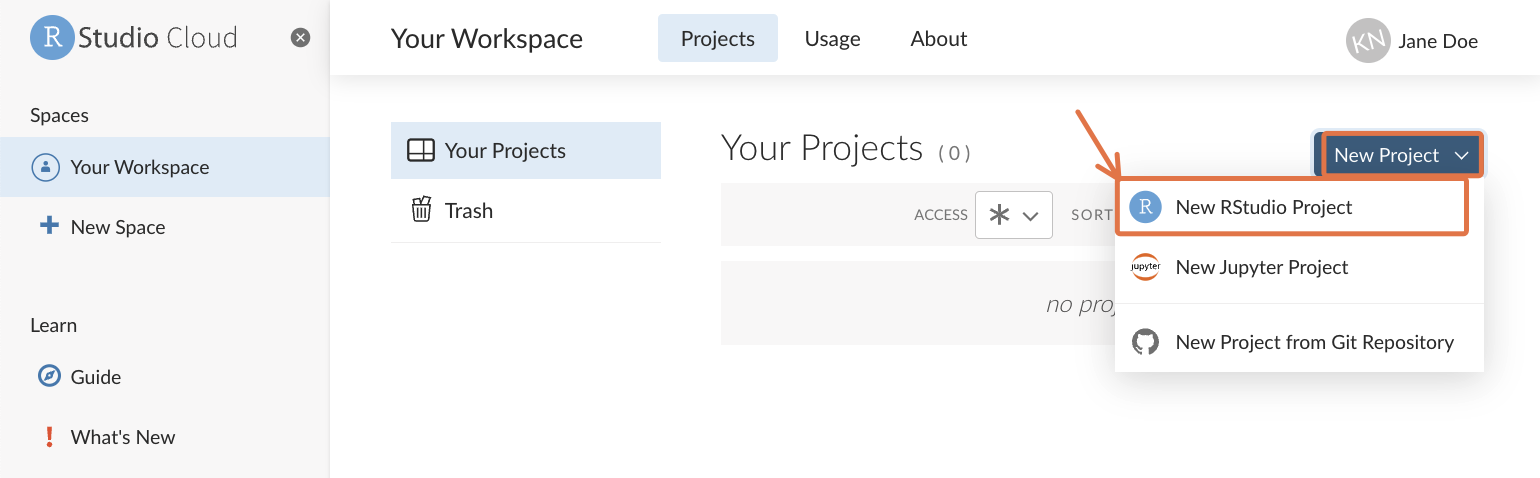
\includegraphics[width=5.51042in,height=\textheight]{images/new_rstudio_project_cloud.png}

You should see a screen like this:

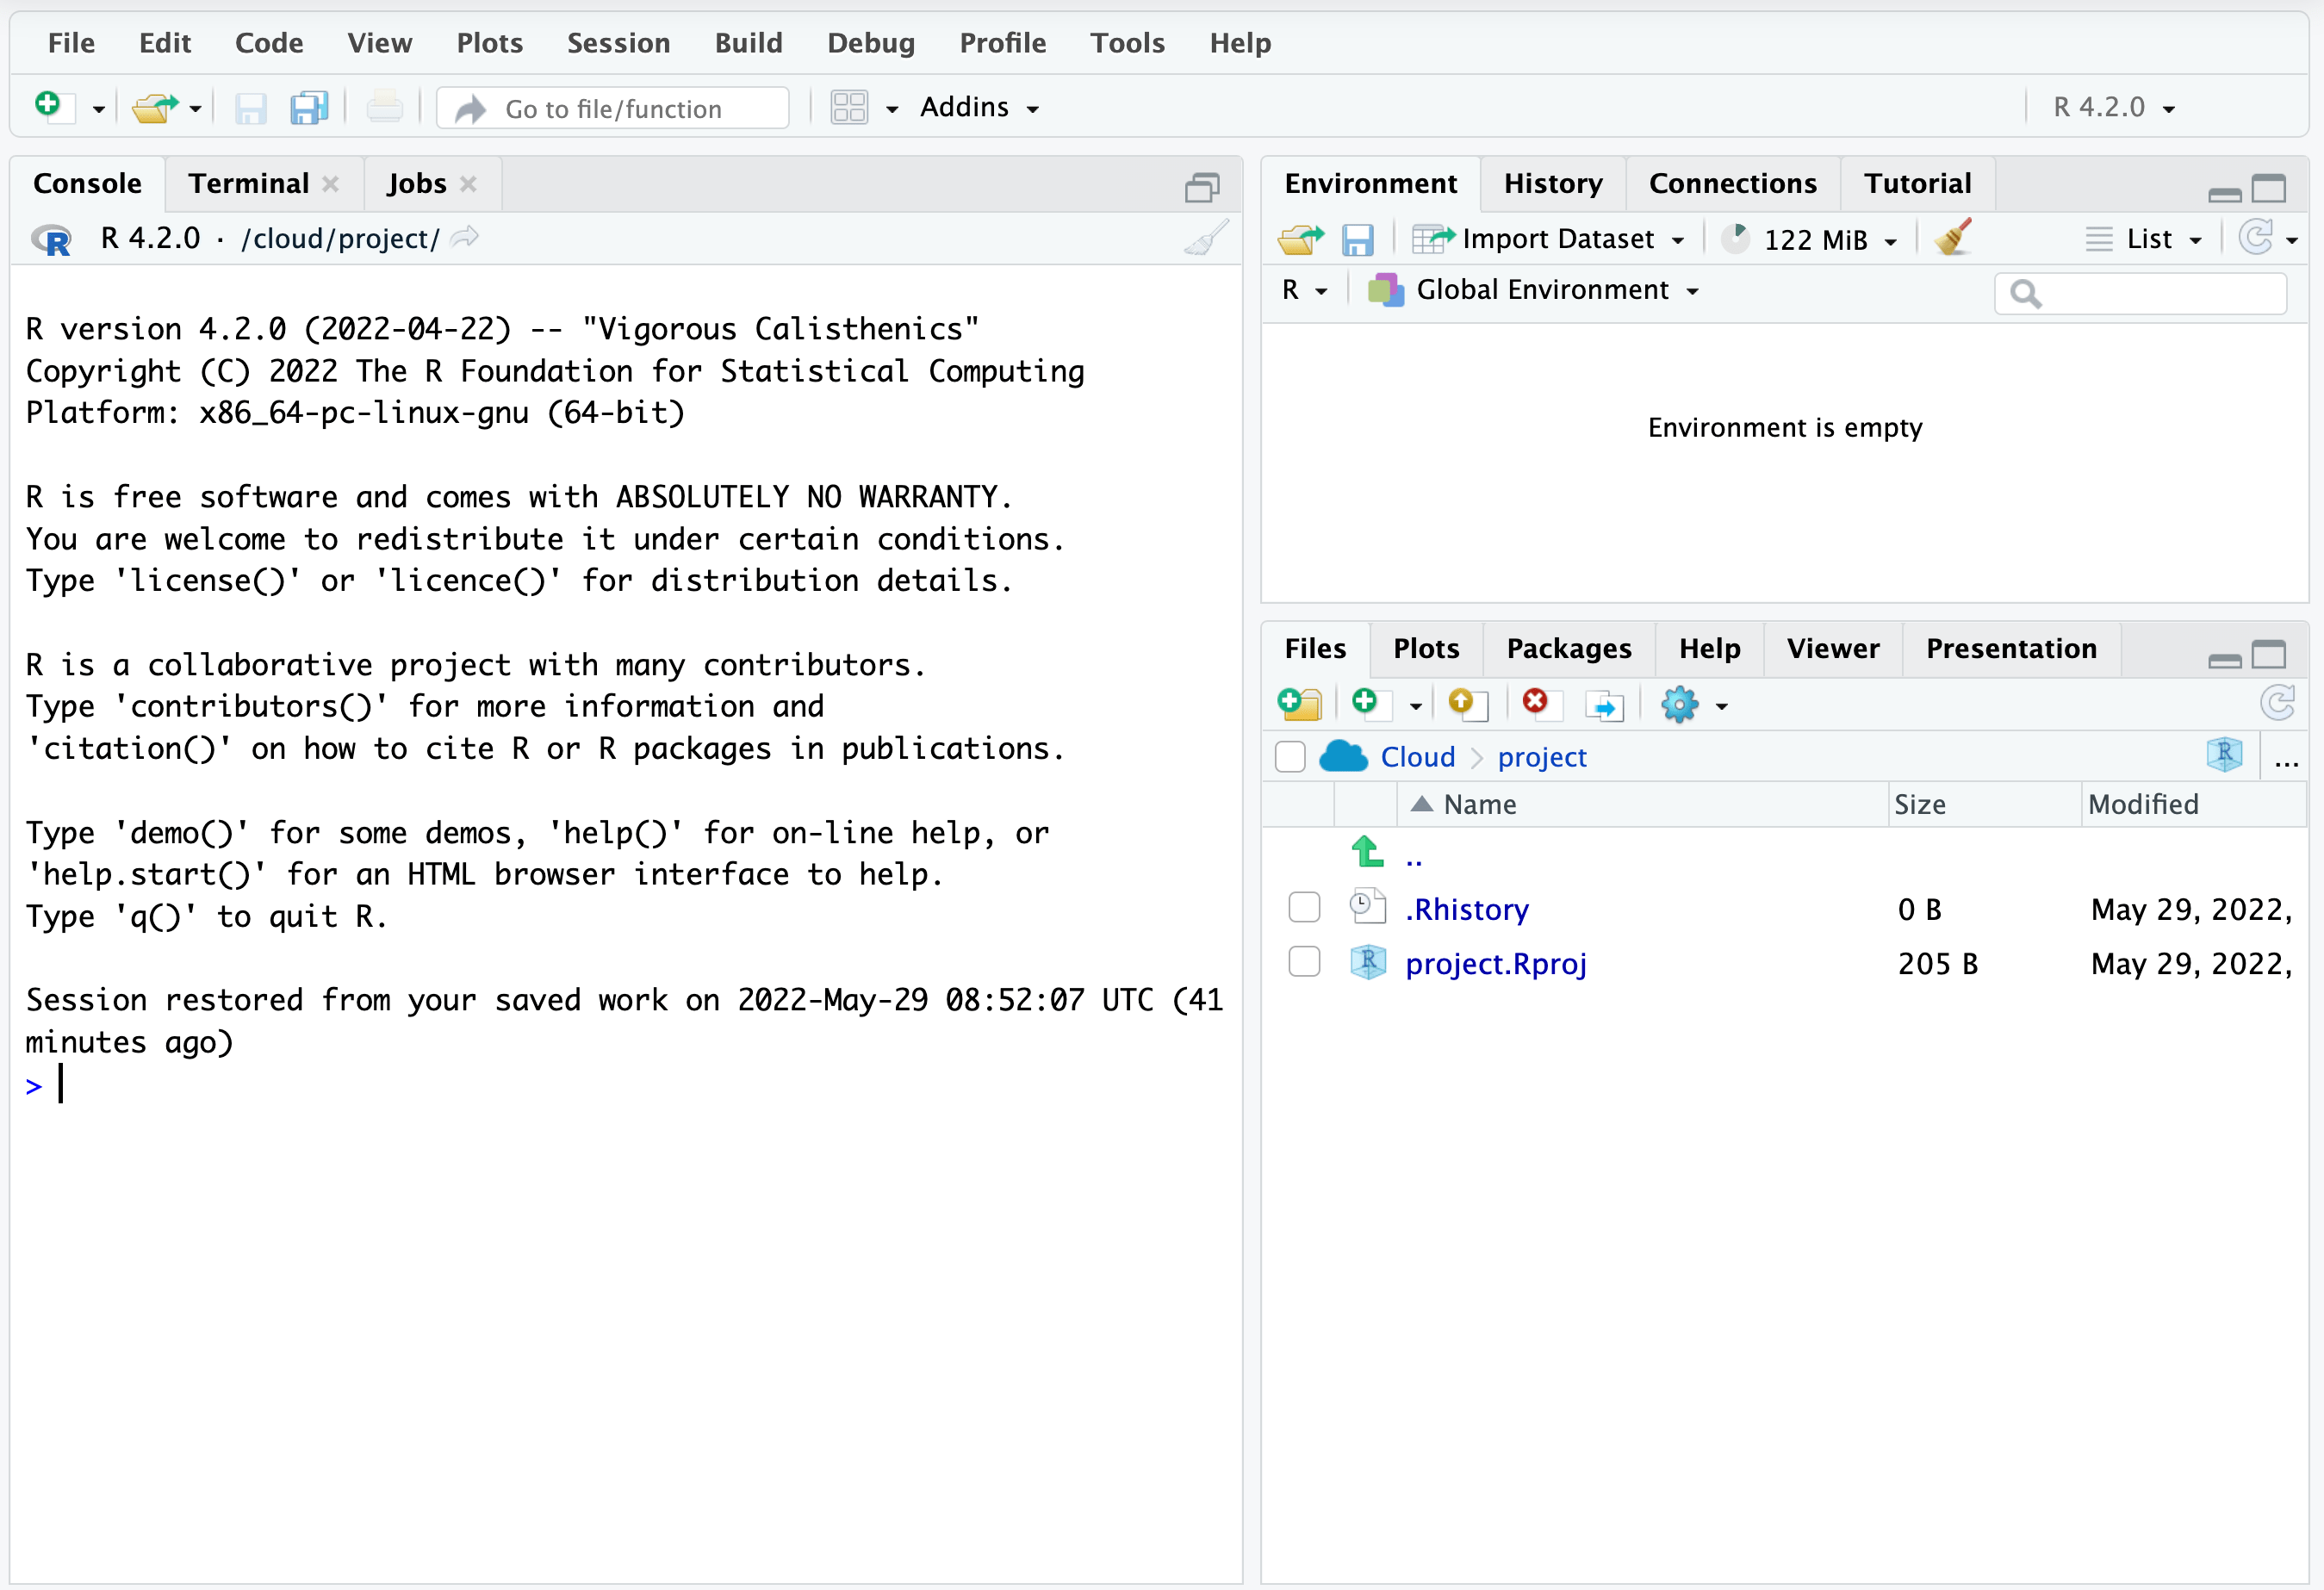
\includegraphics[width=5.5in,height=\textheight]{images/rstudio_cloud_fresh_window.png}

This is RStudio, your new home for a long time to come!

At the top of the screen, rename the project from ``Untitled Project''
to something like ``r\_intro''.

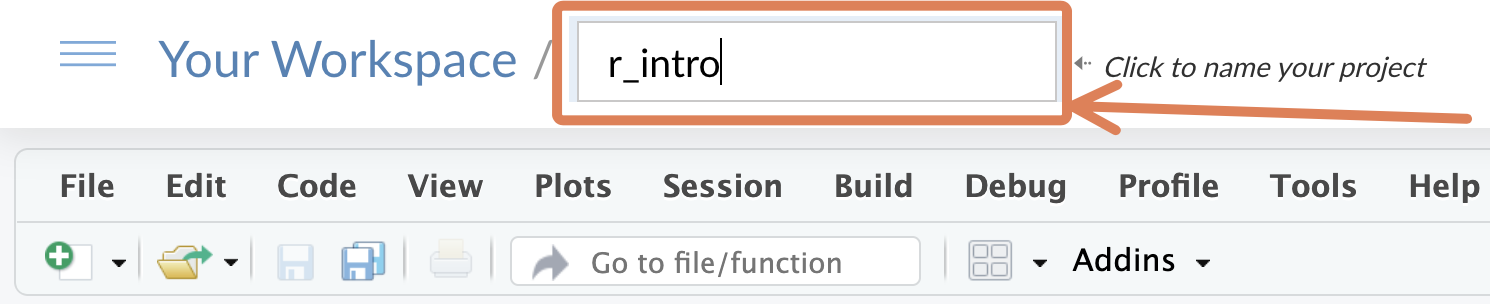
\includegraphics[width=5.48958in,height=\textheight]{images/rstudio_cloud_name_project.png}

You can start using R by typing code into the ``console'' pane on the
left:

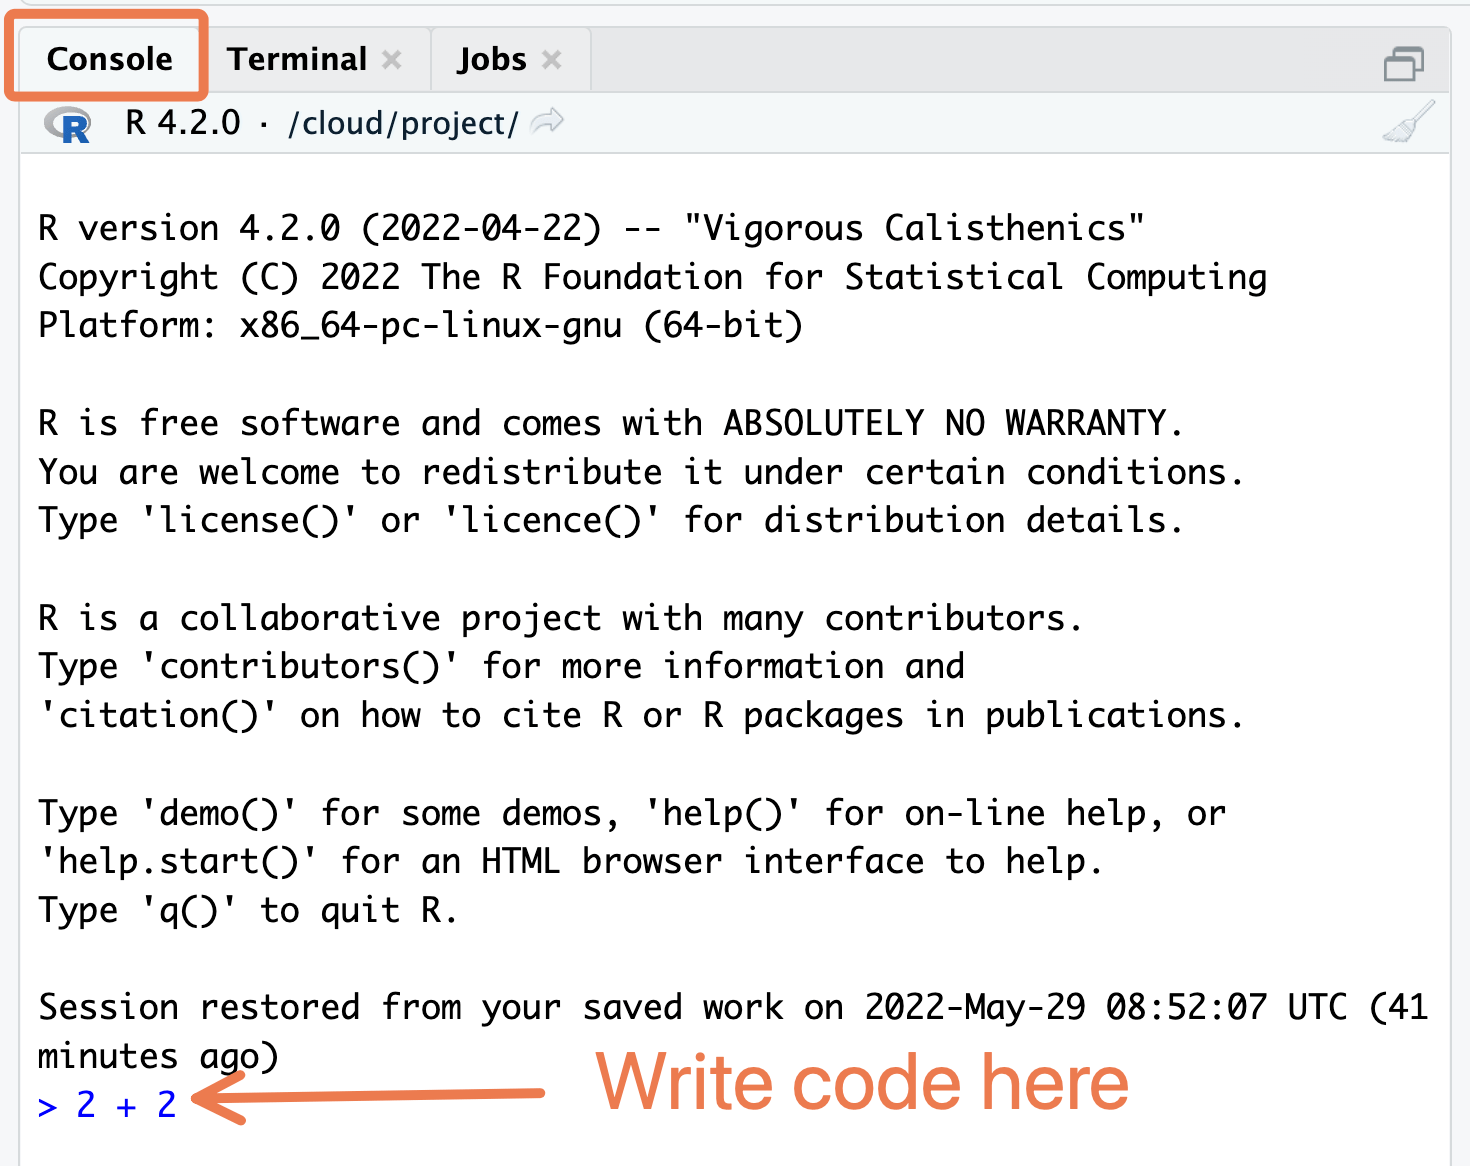
\includegraphics[width=5.4375in,height=\textheight]{images/rstudio_cloud_console.png}

Try using R as a calculator here; type \texttt{2\ +\ 2} and press Enter.

That's it; you're ready to roll. Whenever you want to reopen RStudio,
navigate to rstudio.cloud,

Proceed to the ``wrapping up'' section of the lesson.

\hypertarget{set-up-on-windows}{%
\section{Set up on Windows}\label{set-up-on-windows}}

\hypertarget{download-and-install-r}{%
\subsection{Download and install R}\label{download-and-install-r}}

If you're working on Windows, follow the steps below to download and
install R:

\begin{enumerate}
\def\labelenumi{\arabic{enumi}.}
\item
  Go to \href{https://cran.rstudio.com/}{cran.rstudio.com} to access the
  R installation page. Then click the download link for Windows:

  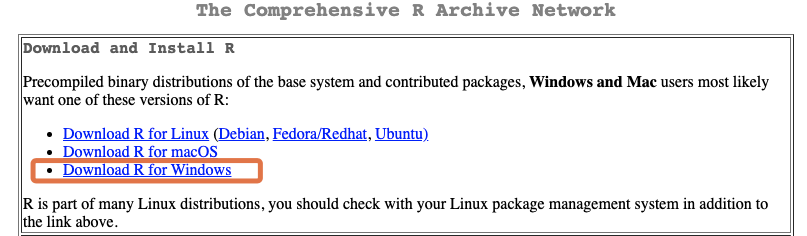
\includegraphics[width=5.59375in,height=\textheight]{images/cran_select_windows.png}
\item
  Choose the ``base'' sub-directory.

  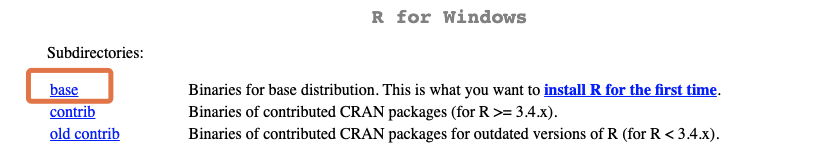
\includegraphics[width=5.91667in,height=\textheight]{images/install_r_windows_base.png}
\item
  Then click on the download link at the top of the page to download the
  latest version of R:

  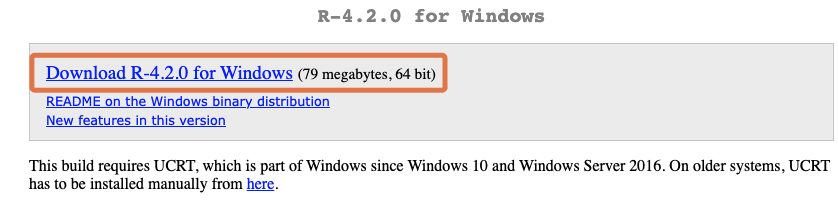
\includegraphics[width=5.92708in,height=\textheight]{images/install_r_windows_download2.png}

  Note that the screenshot above may not show the latest version.
\item
  After the download is finished, click on the downloaded file, then
  follow the instructions on the installation pop-up window. During
  installation, you should not have to change any of the defaults; just
  keep clicking ``Next'' until the installation is done.

  Well done! You should now have R on your computer. But you likely
  won't ever need to interact with R directly. Instead you'll use the
  RStudio IDE to work with R. Follow the instructions in the next
  section to get RStudio.
\end{enumerate}

\hypertarget{download-install-run-rstudio}{%
\subsection{Download, install \& run
RStudio}\label{download-install-run-rstudio}}

To download RStudio, go to
\href{https://www.rstudio.com/products/rstudio/download/\#download}{rstudio.com/products/rstudio/download/\#download}
and download the Windows version.

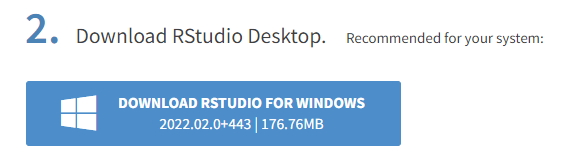
\includegraphics[width=4.16667in,height=\textheight]{images/install_rstudio_button_windows.png}

After the download is finished, click on the downloaded file and follow
the installation instructions.

Once installed, RStudio can be opened like any application on your
computer: press the Windows key to bring up the Start menu, and search
for ``rstudio''. Click to to open the app:

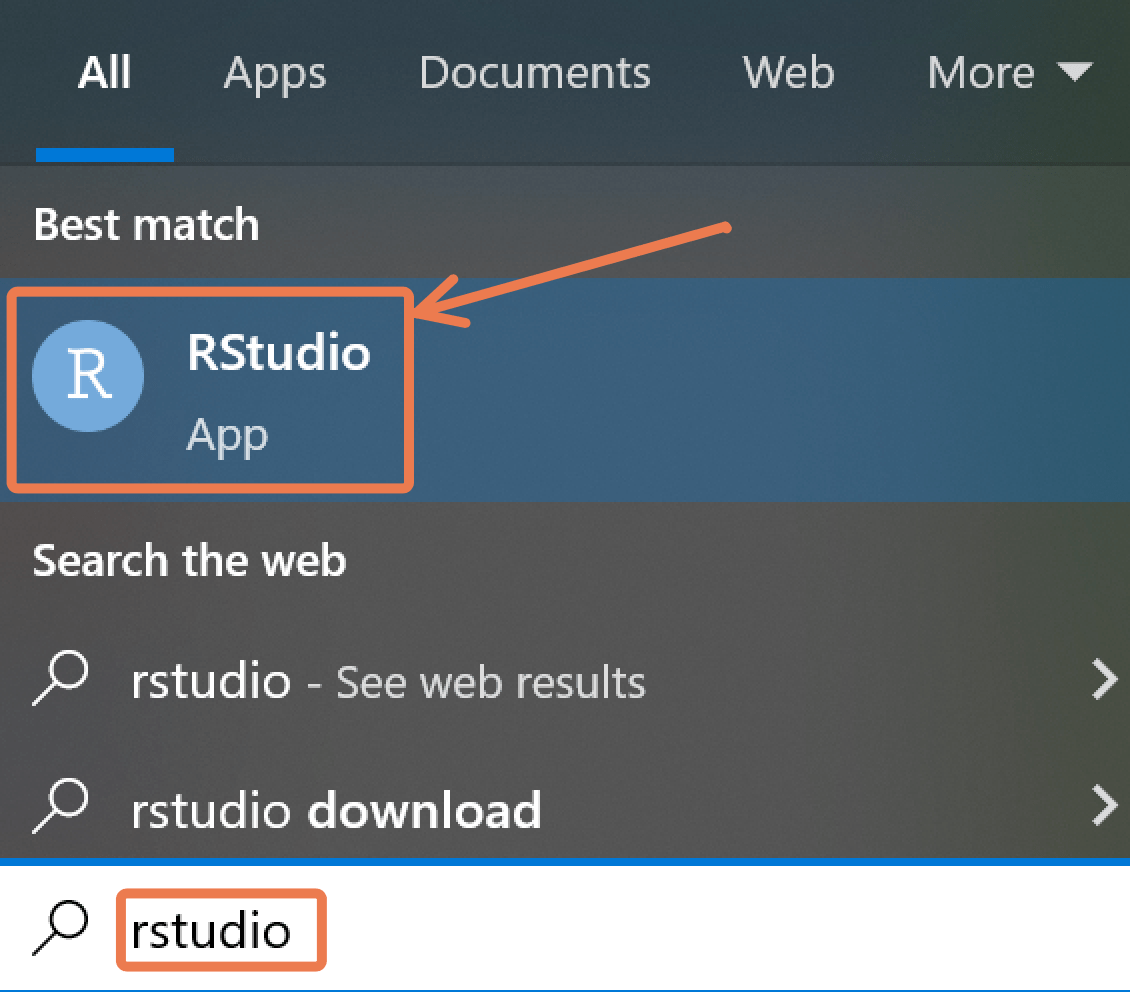
\includegraphics[width=4.16667in,height=\textheight]{images/open_rstudio_windows.png}

You should see a window like this:

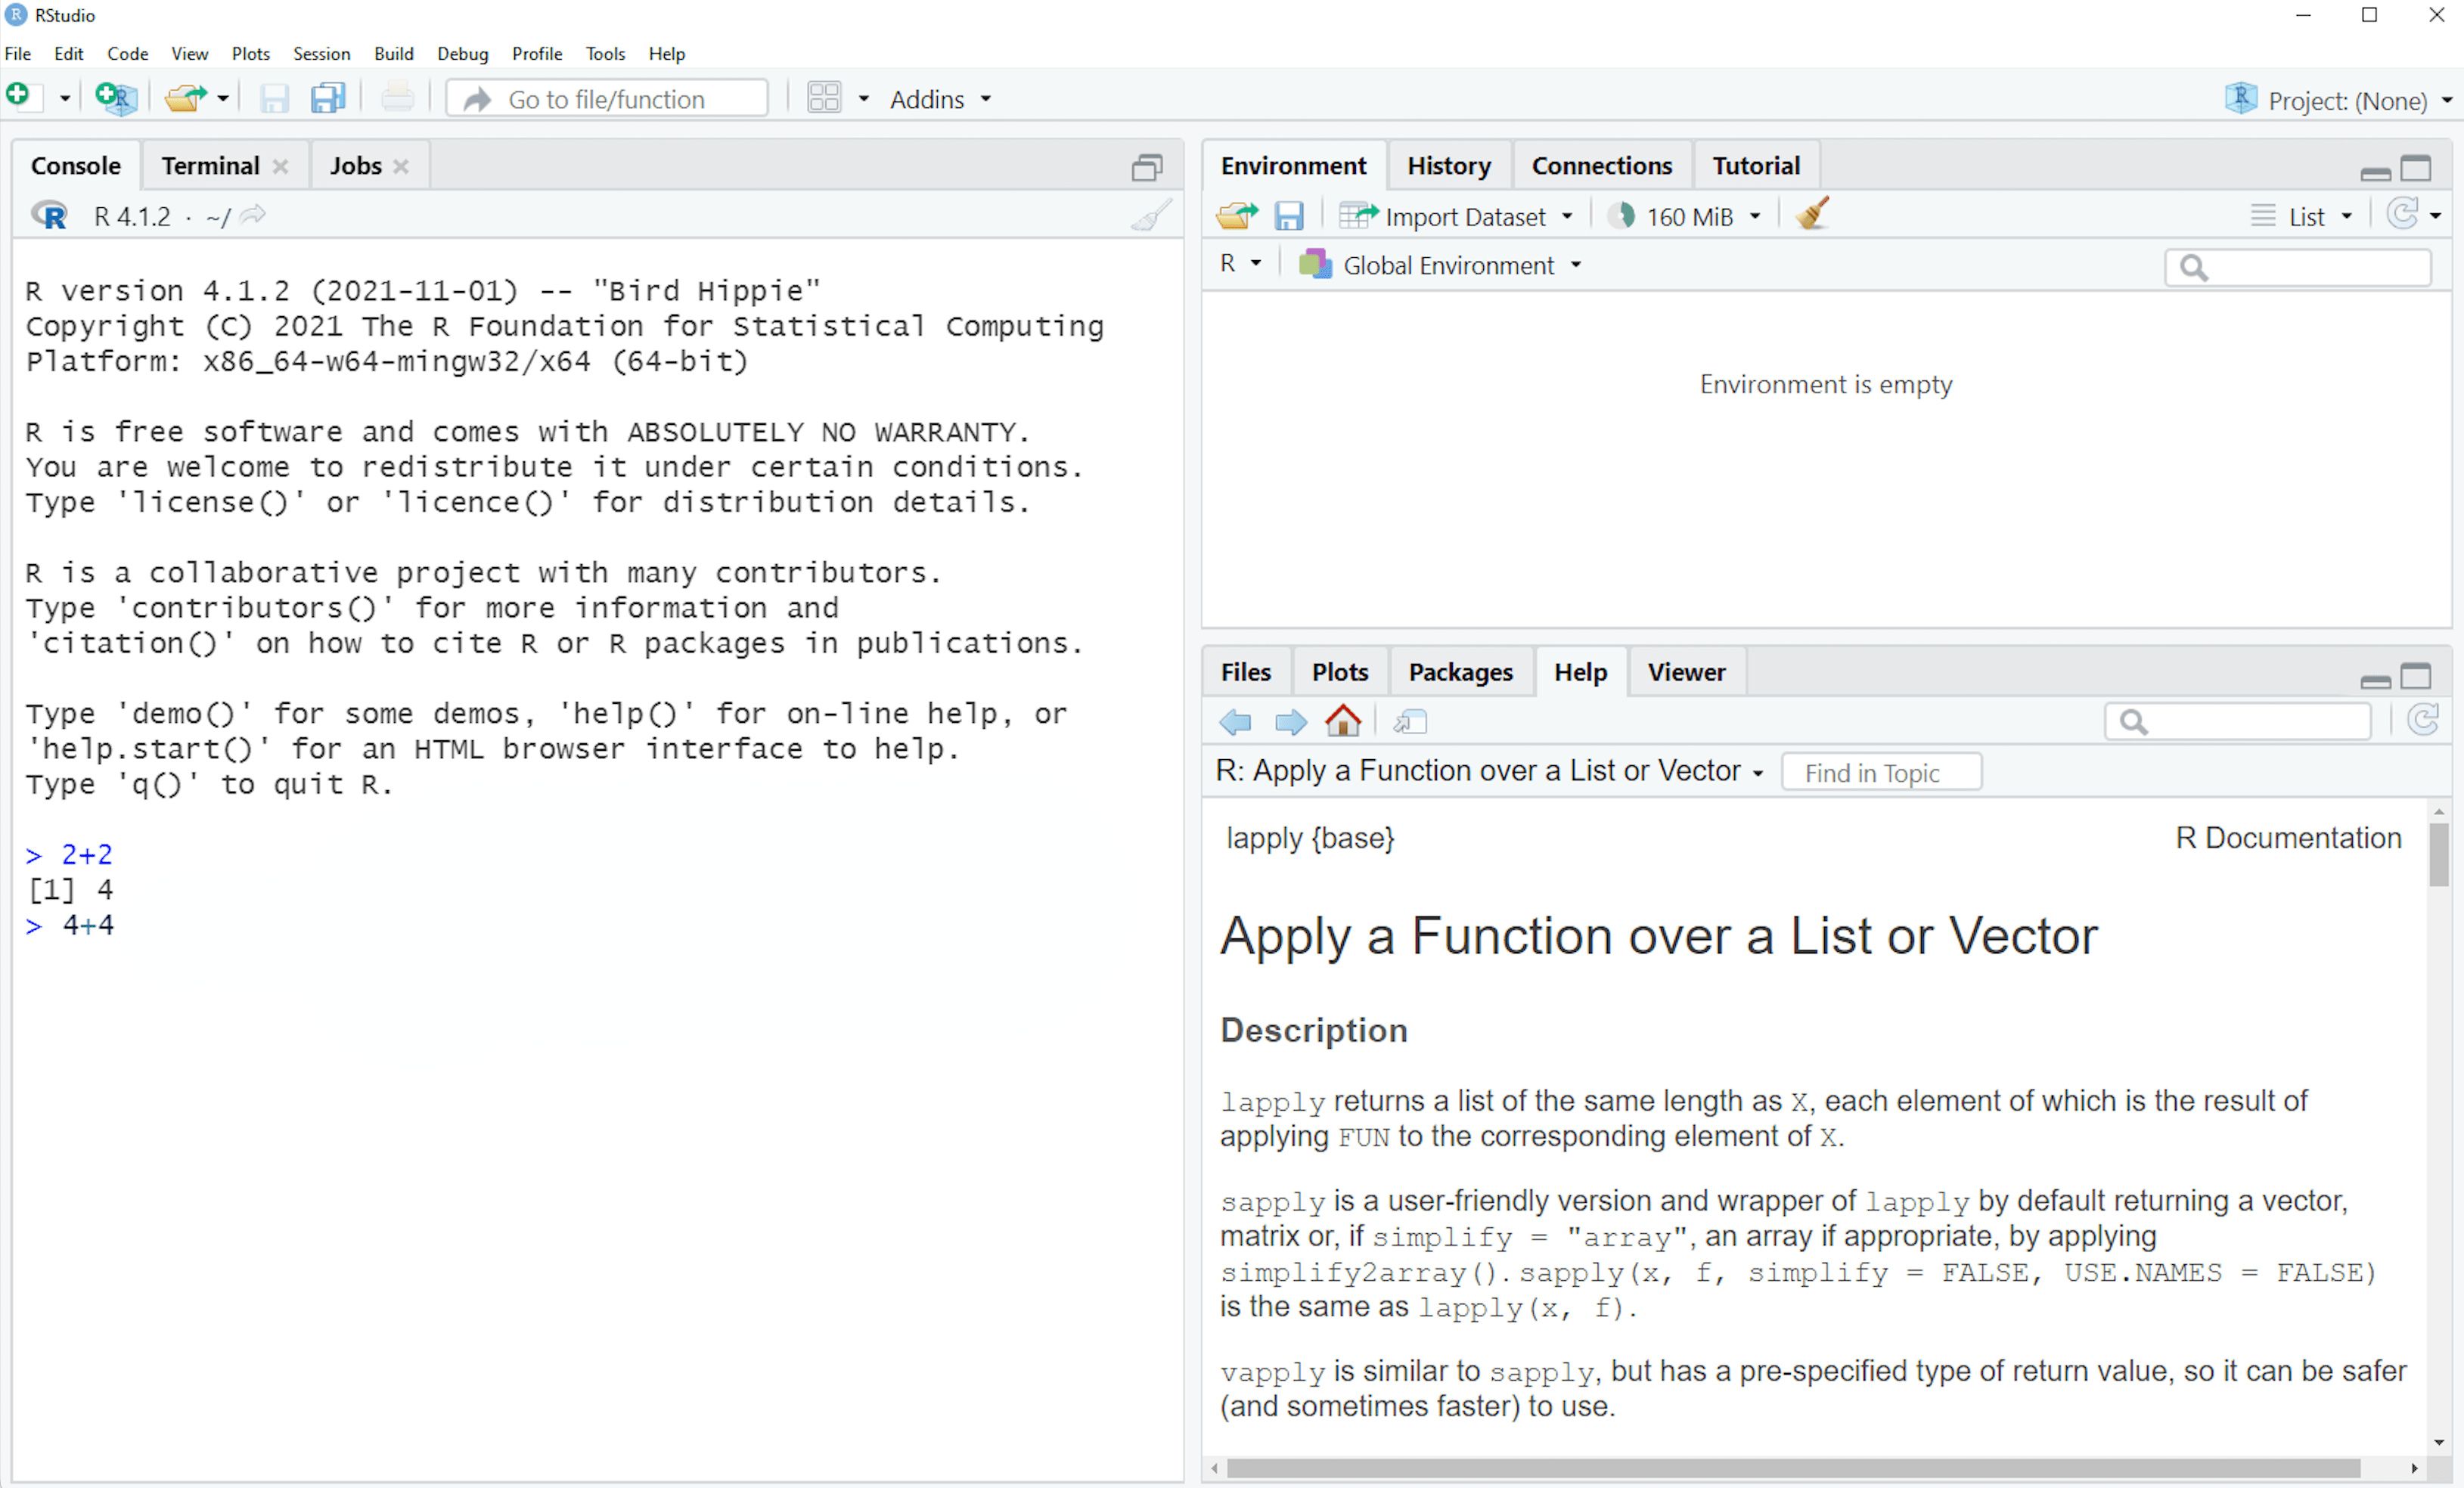
\includegraphics[width=6.1875in,height=\textheight]{images/rstudio_first_view_windows.png}

This is RStudio, your new home for a long time to come!

You can start using R by typing code into the ``console'' pane on the
left:

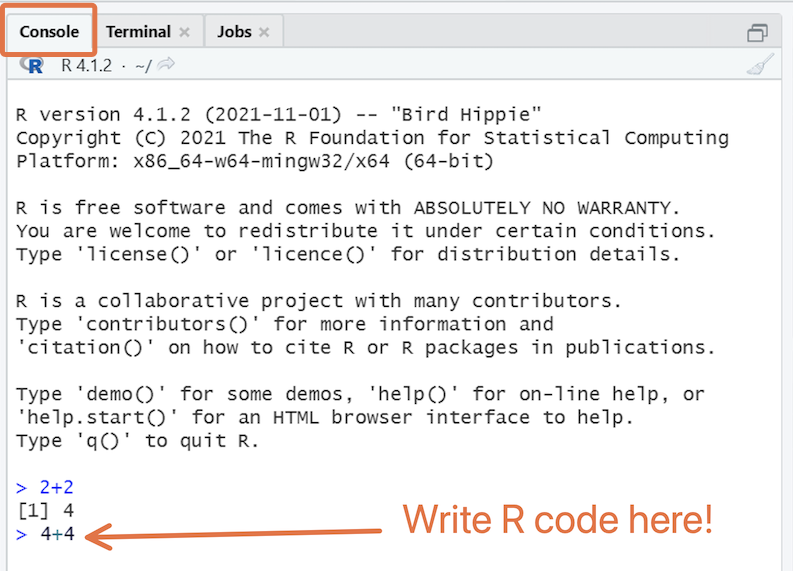
\includegraphics[width=5.20833in,height=\textheight]{images/windows_write_code_here.png}

Try using R as a calculator here; type \texttt{2\ +\ 2} and press Enter.

That's it; you're ready to roll. Proceed to the ``wrapping up'' section
of the lesson.

\hypertarget{set-up-on-macos}{%
\section{Set up on macOS}\label{set-up-on-macos}}

\hypertarget{download-and-install-r-1}{%
\subsection{Download and install R}\label{download-and-install-r-1}}

If you're working on macOS, follow the steps below to download and
install R:

\begin{enumerate}
\def\labelenumi{\arabic{enumi}.}
\item
  Go to \href{https://cran.rstudio.com/}{cran.rstudio.com} to access the
  R installation page. Then click the link for macOS:

  
\includegraphics[width=4.46875in,height=\textheight]{images/install_r_select_mac.png}
\item
  Download and install the relevant R version for your Mac. For most
  people, the first option under ``Latest release'' will be the one to
  get.

  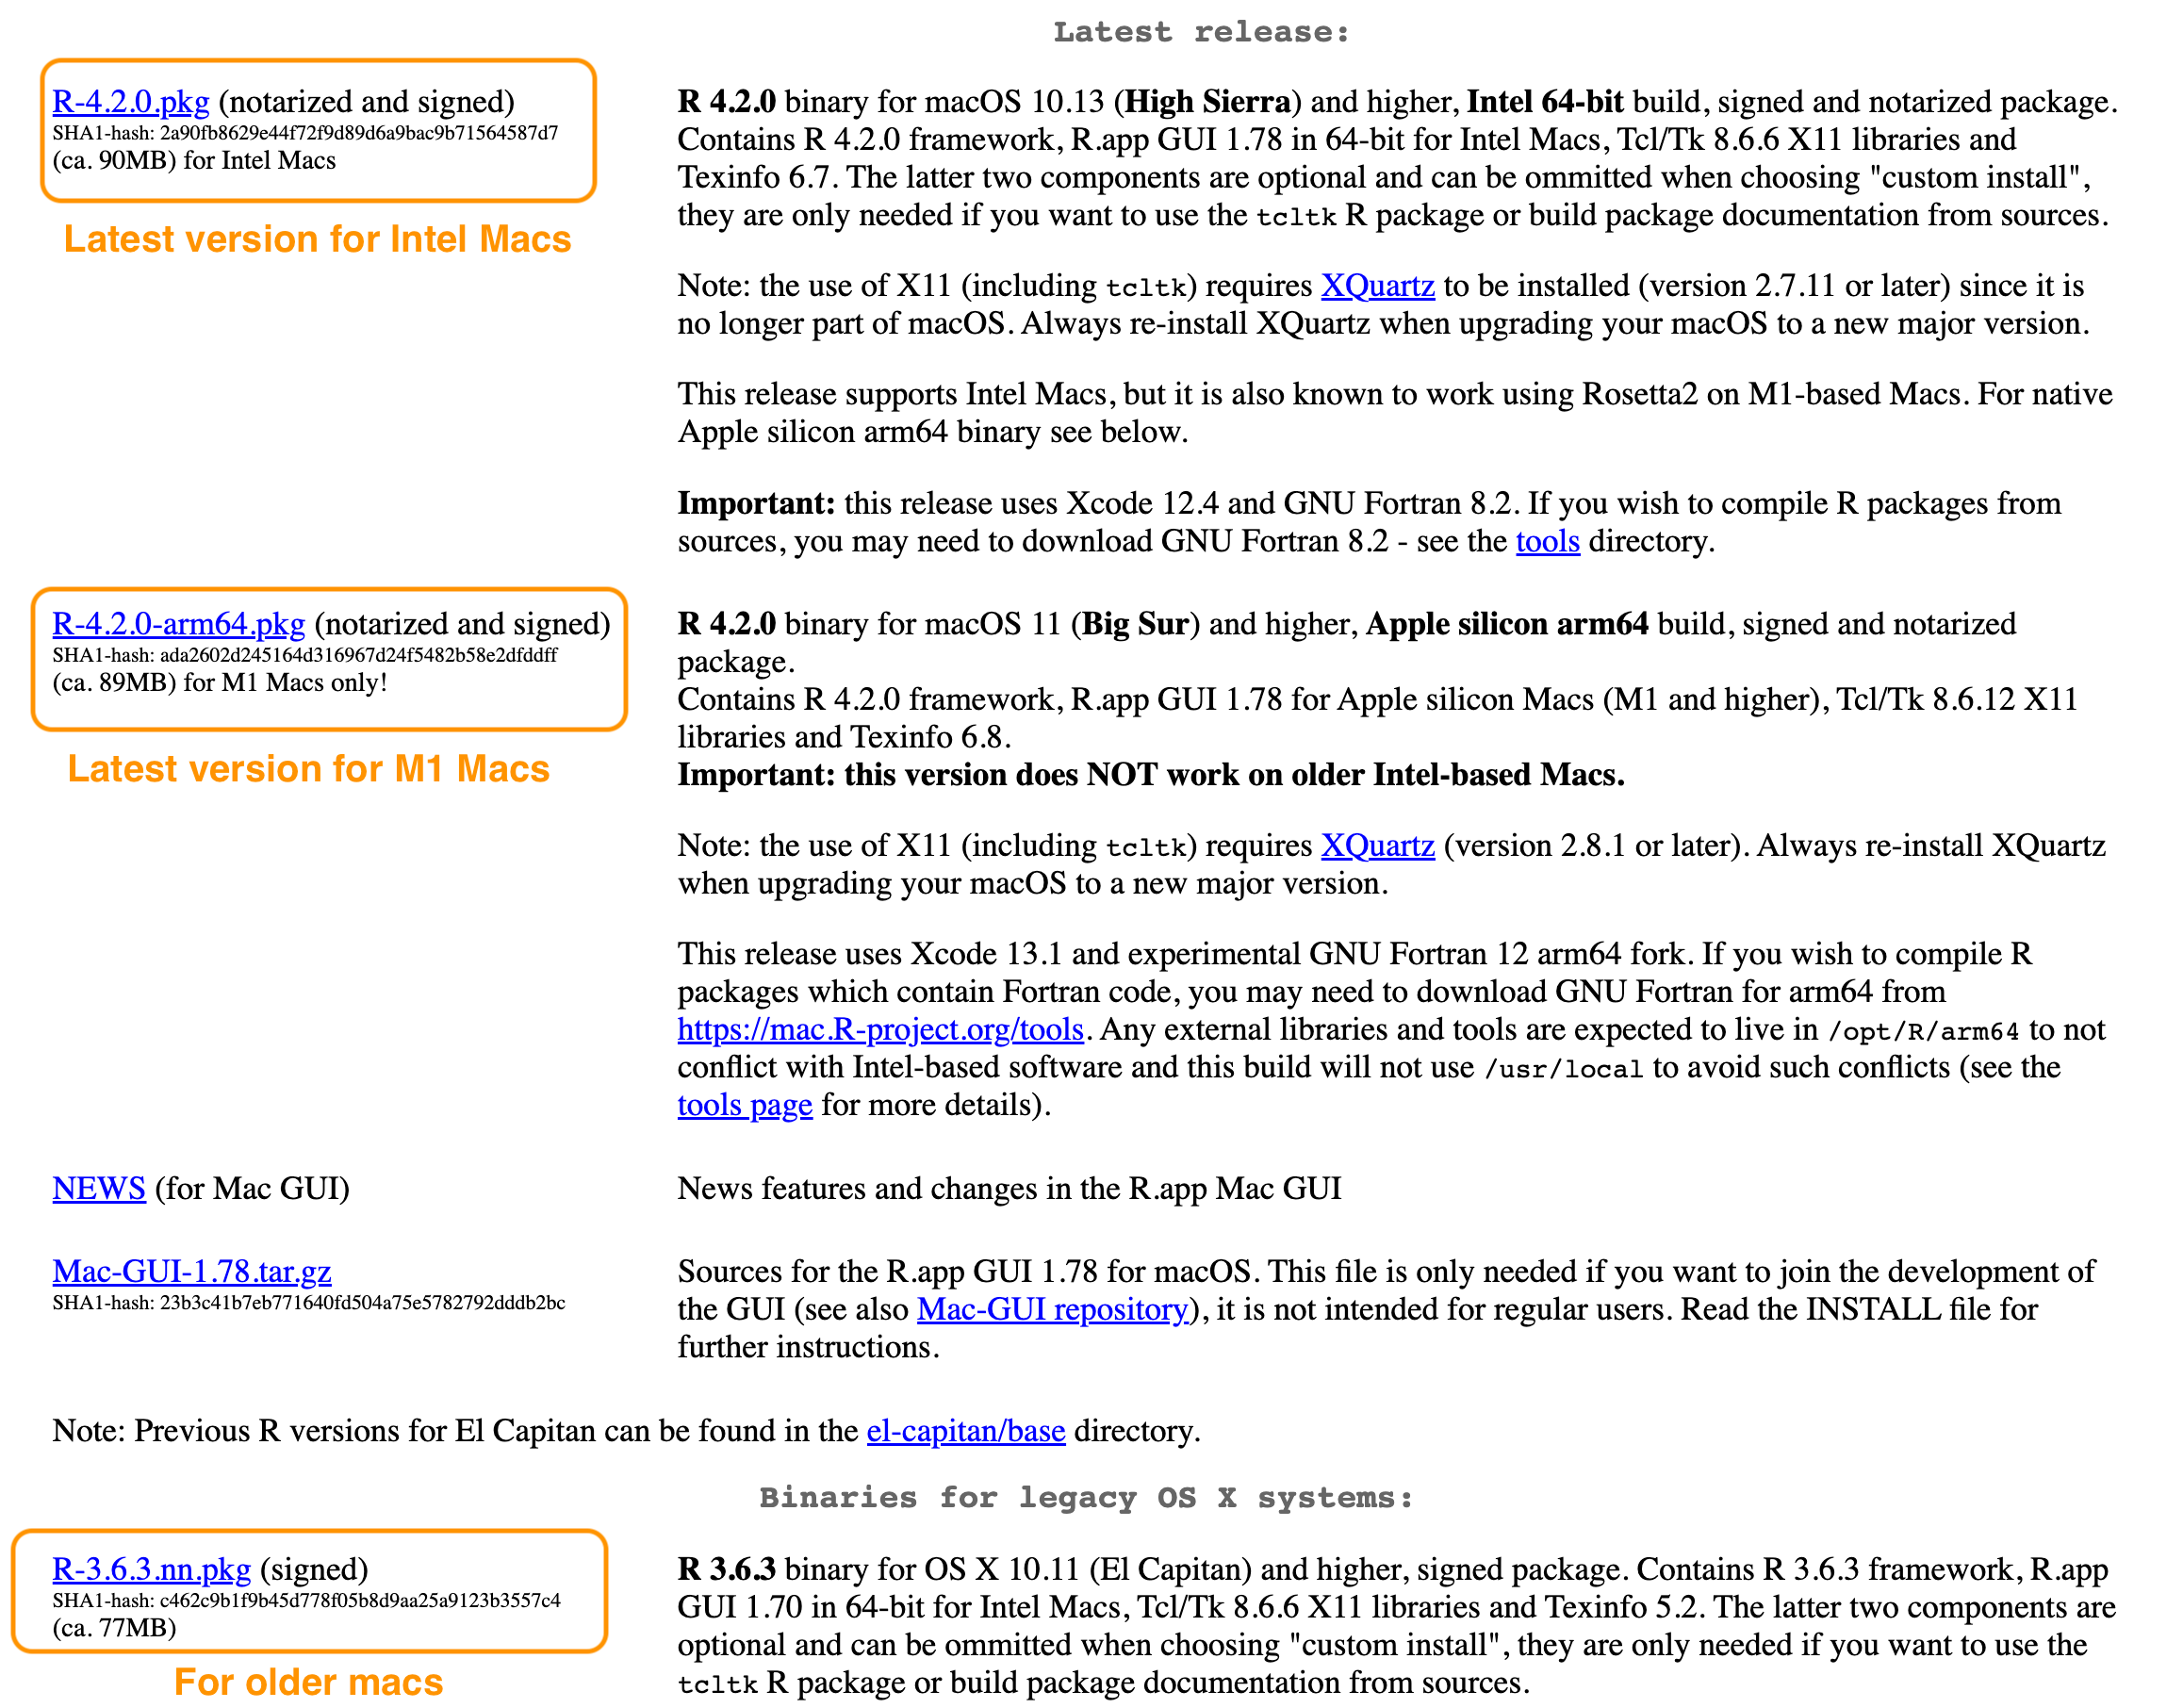
\includegraphics[width=4.39583in,height=\textheight]{images/r_mac_select_version.png}
\item
  After the download is finished, click on the downloaded file, then
  follow the instructions on the installation pop-up window.
\end{enumerate}

Well done! You should now have R on your computer. But you likely won't
ever need to interact with R directly. Instead you'll use the RStudio
IDE to work with R. Follow the instructions in the next section to get
RStudio.

\hypertarget{download-install-run-rstudio-1}{%
\subsection{Download, install \& run
RStudio}\label{download-install-run-rstudio-1}}

To download RStudio, go to
\href{https://www.rstudio.com/products/rstudio/download/\#download}{rstudio.com/products/rstudio/download/\#download}
and download the version for macOS.

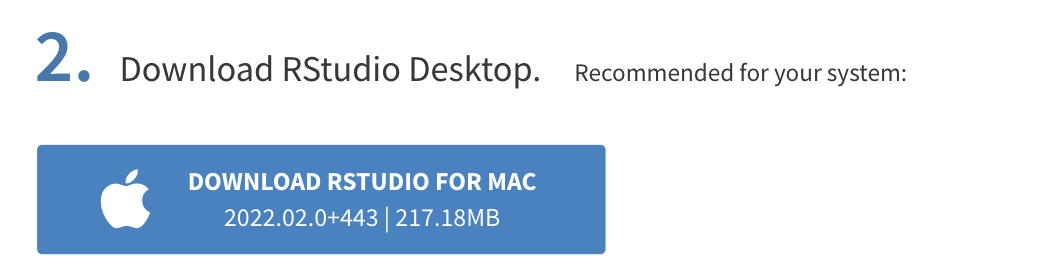
\includegraphics[width=4.16667in,height=\textheight]{images/download_rstudio_button_mac.png}

After the download is finished, click on the downloaded file and follow
the installation instructions.

Once installed, RStudio can be opened like any application on your
computer: Press \texttt{Command} + \texttt{Space} to open Spotlight,
then search for ``rstudio''. Click to open the app.


\includegraphics[width=4.16667in,height=\textheight]{images/mac_spotlight_rstudio.png}

You should see a window like this:

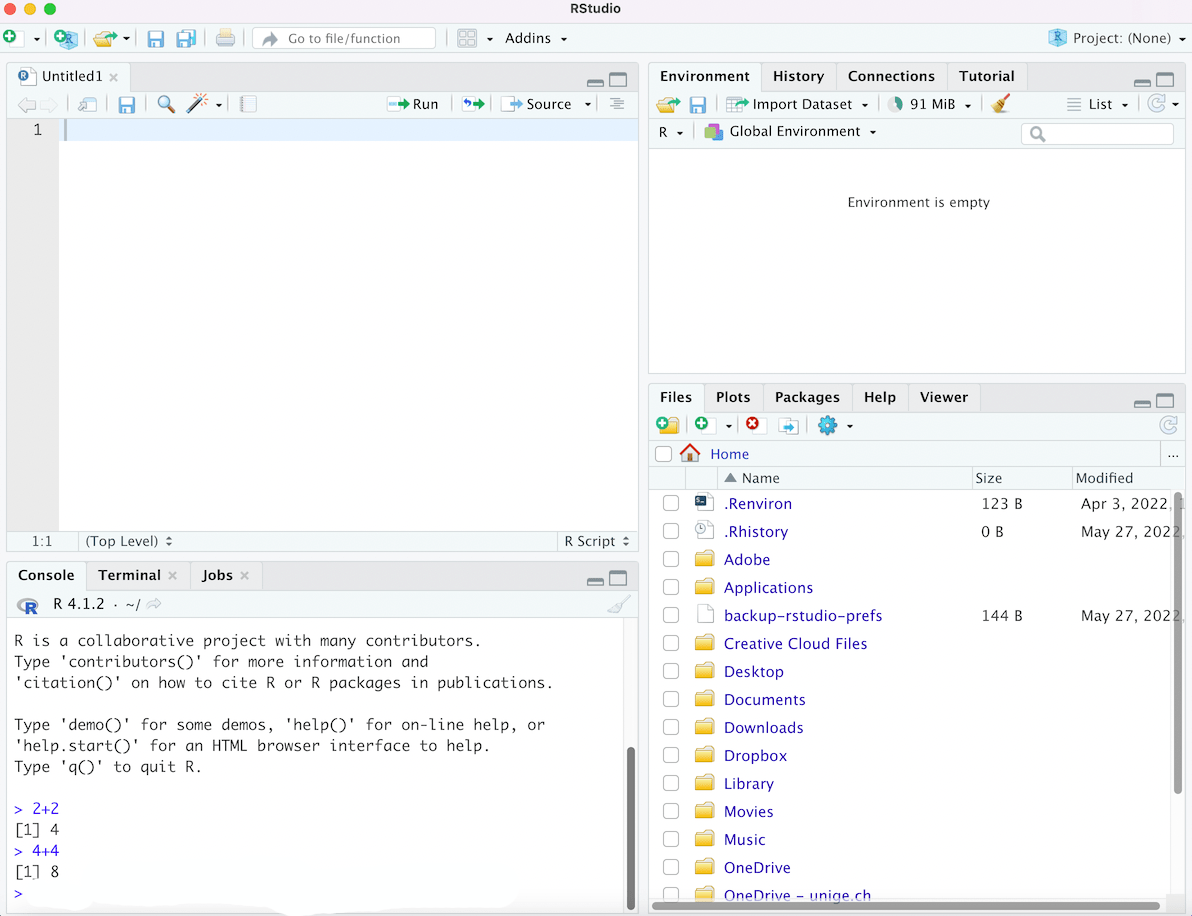
\includegraphics[width=5.375in,height=\textheight]{images/mac_rstudio_window.png}

This is RStudio, your new home for a long time to come!

You can start using R by typing code into the ``console'' pane on the
left:

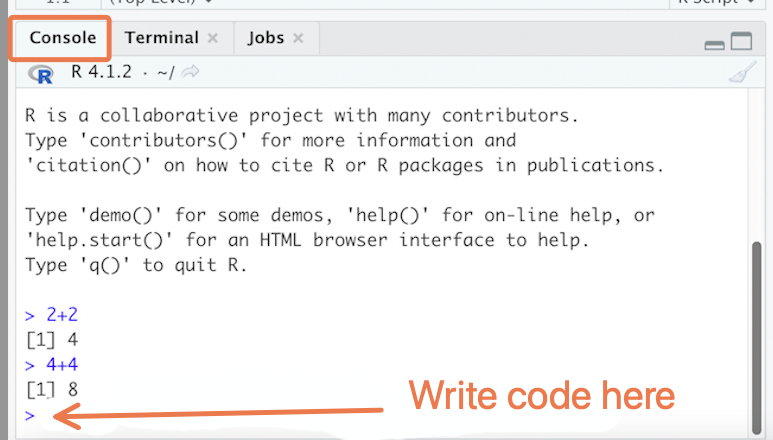
\includegraphics[width=5.20833in,height=\textheight]{images/mac_write_code_here.png}

Try using R as a calculator here; type \texttt{2\ +\ 2} and press Enter.

\hypertarget{wrap-up}{%
\section{Wrap up}\label{wrap-up}}

You should now have access to R and RStudio, so you're all set to begin
the journey of learning to use these immensely powerful tools. See you
in the next session!

\hypertarget{references}{%
\section*{References}\label{references}}

\markright{References}

Some material in this lesson was adapted from the following sources:

\begin{itemize}
\tightlist
\item
  Nordmann, Emily, and Heather Cleland-Woods. \emph{Chapter 2
  Programming Basics \textbar{} Data Skills}.
  \emph{psyteachr.github.io},
  \url{https://psyteachr.github.io/data-skills-v1/programming-basics.html}
  Accessed 23 Feb.~2022.
\end{itemize}

\bookmarksetup{startatroot}

\hypertarget{setting-up-r-and-rstudio-1}{%
\chapter{Setting up R and RStudio}\label{setting-up-r-and-rstudio-1}}

\begin{center}\rule{0.5\linewidth}{0.5pt}\end{center}

\hypertarget{learning-objective-1}{%
\section*{Learning objective}\label{learning-objective-1}}

\markright{Learning objective}

\begin{enumerate}
\def\labelenumi{\arabic{enumi}.}
\tightlist
\item
  You can access R and RStudio, either through RStudio.cloud or by
  downloading and installing these software to your computer.
\end{enumerate}

\hypertarget{introduction-2}{%
\section{Introduction}\label{introduction-2}}

To start you off on your R journey, we'll need to set you up with the
required software, R and RStudio. \textbf{R} is the programming language
that you'll use write code, while \textbf{RStudio} is an integrated
development environment (IDE) that makes working with R easier.

\hypertarget{working-locally-vs.-on-the-cloud-1}{%
\section{Working locally vs.~on the
cloud}\label{working-locally-vs.-on-the-cloud-1}}

There are two main ways that you can access and work with R and RStudio:
download them to your computer, or use a web server to access them on
the cloud.

Using R and RStudio on the cloud is the less common option, but it may
be the right choice if you are just getting started with programming,
and you do not yet want to worry about installing software. You may also
prefer the cloud option if your local computer is old, slow, or
otherwise unfit for running R.

Below, we go through the setup process for RStudio Cloud, Rstudio on
Windows and RStudio on macOS separately. Jump to the section that is
relevant for you!

\begin{tcolorbox}[enhanced jigsaw, colframe=quarto-callout-caution-color-frame, rightrule=.15mm, opacityback=0, breakable, coltitle=black, colbacktitle=quarto-callout-caution-color!10!white, bottomrule=.15mm, leftrule=.75mm, toprule=.15mm, arc=.35mm, bottomtitle=1mm, colback=white, left=2mm, opacitybacktitle=0.6, titlerule=0mm, title=\textcolor{quarto-callout-caution-color}{\faFire}\hspace{0.5em}{Watch Out}, toptitle=1mm]

RStudio cloud will only give you 25 free project hours per month. After
that, you will need to upgrade to a paid plan. If you think you'll need
more than 25 hours per month, you may want to avoid this option.

\end{tcolorbox}

\hypertarget{rstudio-on-the-cloud-1}{%
\section{RStudio on the cloud}\label{rstudio-on-the-cloud-1}}

If you'll be working on the cloud, follow the steps below:

\begin{enumerate}
\def\labelenumi{\arabic{enumi}.}
\item
  Go to the website \href{https://rstudio.cloud}{rstudio.cloud} and
  follow the instructions to sign up for a free account. (We recommend
  signing up with Google if you have a Google account, so you don't need
  to remember any new passwords).
\item
  Once you're done, click on the ``New Project'' icon at the top right,
  and select ``New RStudio Project''.
\end{enumerate}

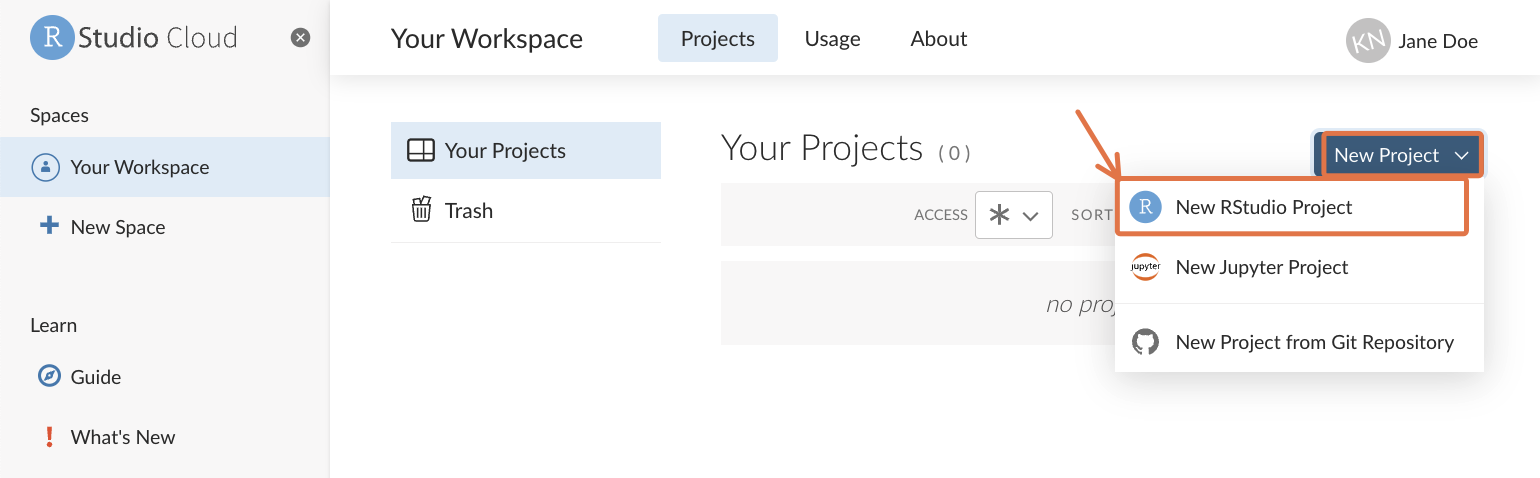
\includegraphics[width=5.51042in,height=\textheight]{images/new_rstudio_project_cloud.png}

You should see a screen like this:

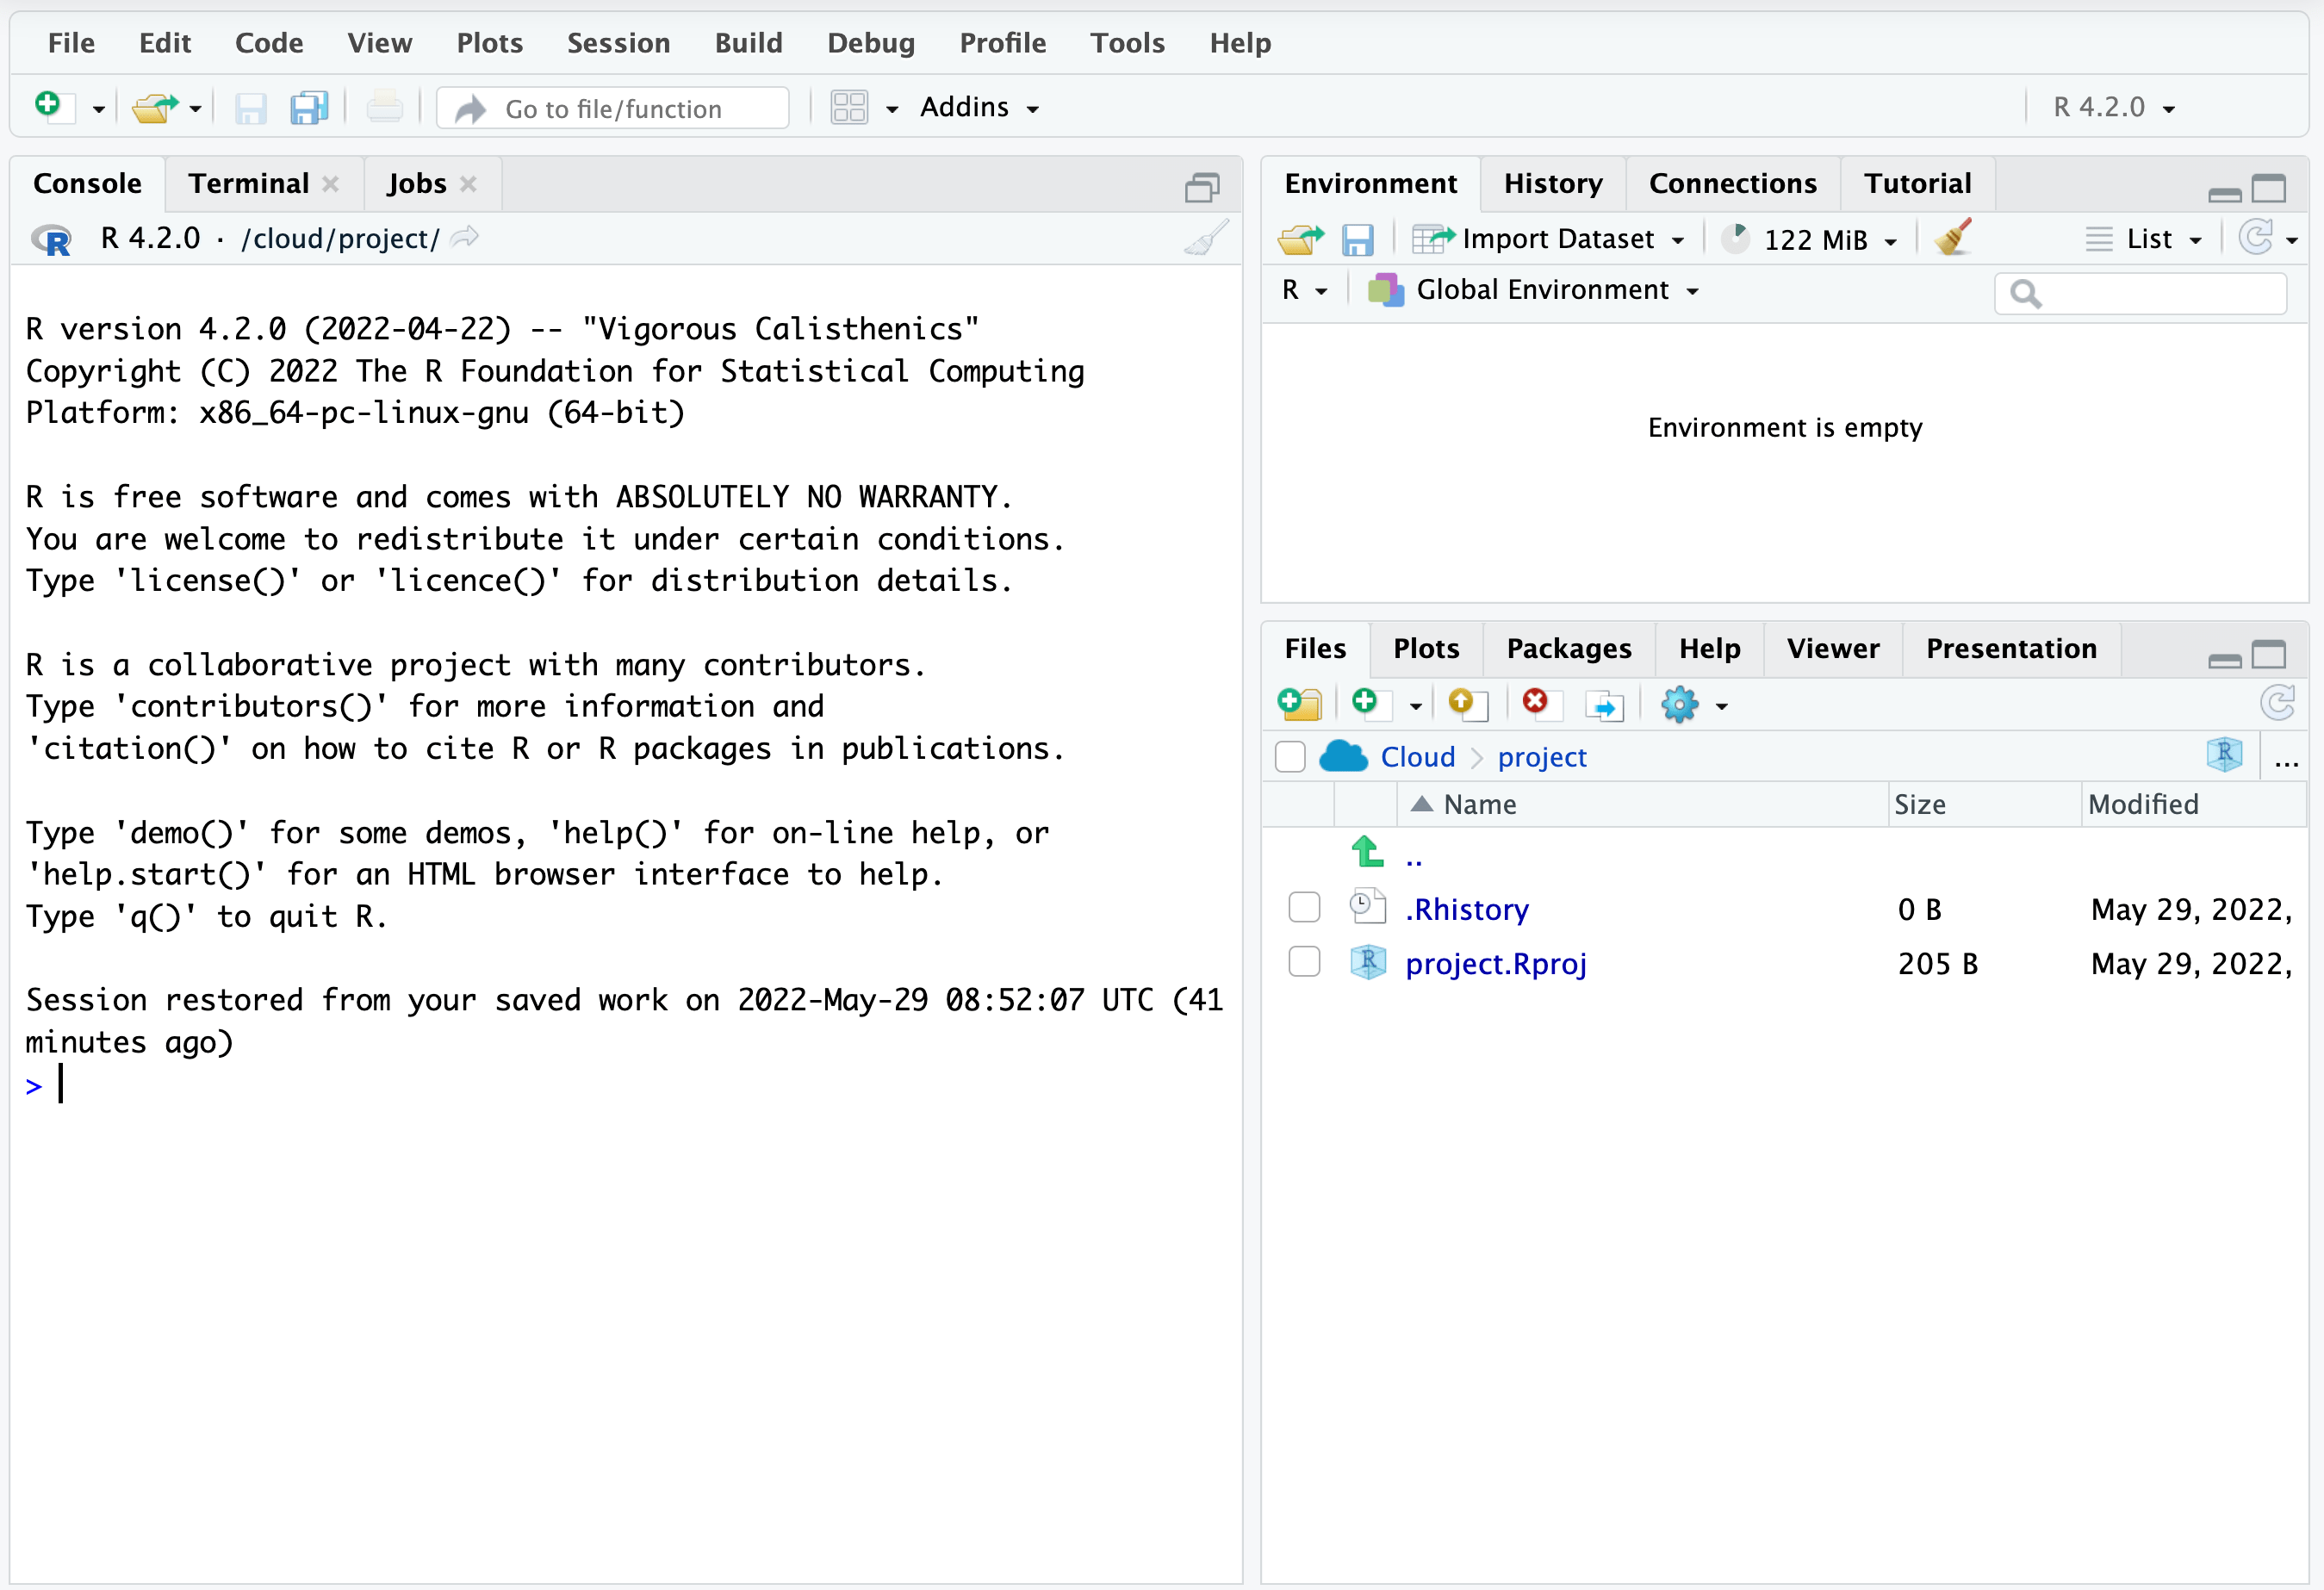
\includegraphics[width=5.5in,height=\textheight]{images/rstudio_cloud_fresh_window.png}

This is RStudio, your new home for a long time to come!

At the top of the screen, rename the project from ``Untitled Project''
to something like ``r\_intro''.

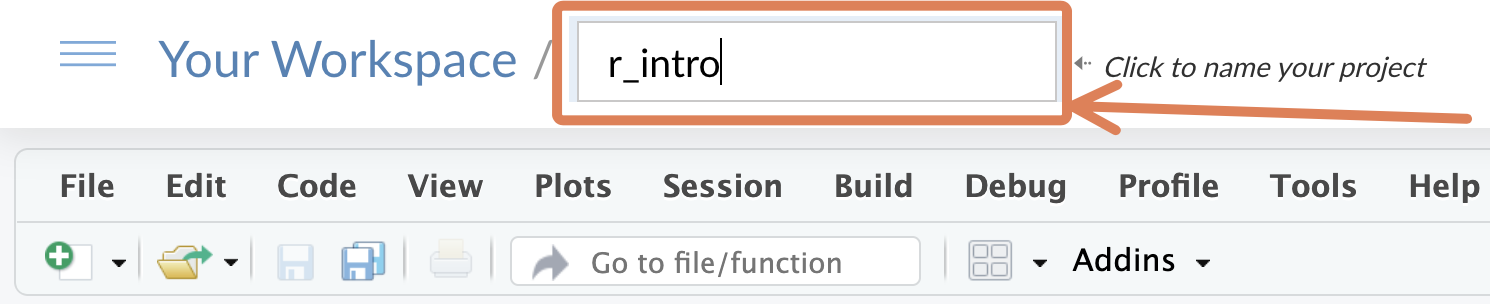
\includegraphics[width=5.48958in,height=\textheight]{images/rstudio_cloud_name_project.png}

You can start using R by typing code into the ``console'' pane on the
left:

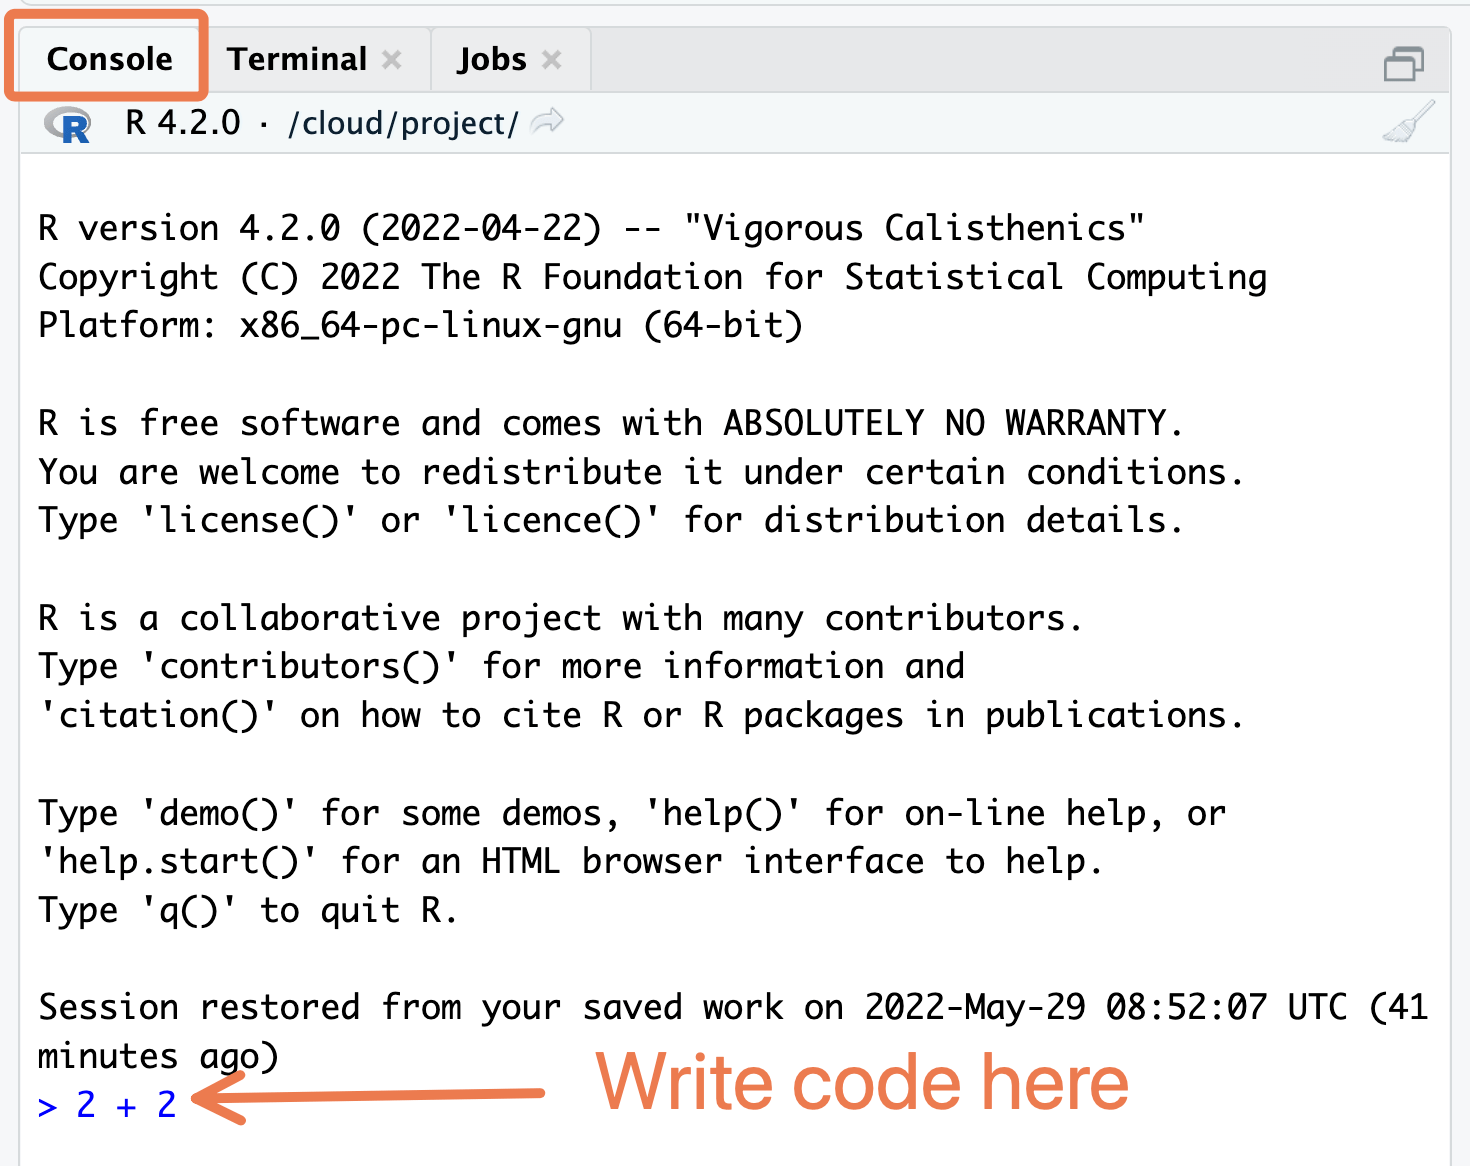
\includegraphics[width=5.4375in,height=\textheight]{images/rstudio_cloud_console.png}

Try using R as a calculator here; type \texttt{2\ +\ 2} and press Enter.

That's it; you're ready to roll. Whenever you want to reopen RStudio,
navigate to rstudio.cloud,

Proceed to the ``wrapping up'' section of the lesson.

\hypertarget{set-up-on-windows-1}{%
\section{Set up on Windows}\label{set-up-on-windows-1}}

\hypertarget{download-and-install-r-2}{%
\subsection{Download and install R}\label{download-and-install-r-2}}

If you're working on Windows, follow the steps below to download and
install R:

\begin{enumerate}
\def\labelenumi{\arabic{enumi}.}
\item
  Go to \href{https://cran.rstudio.com/}{cran.rstudio.com} to access the
  R installation page. Then click the download link for Windows:

  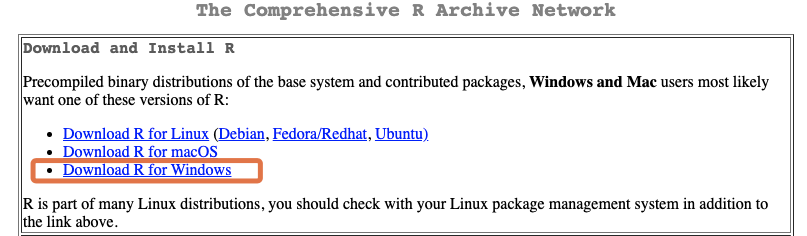
\includegraphics[width=5.59375in,height=\textheight]{images/cran_select_windows.png}
\item
  Choose the ``base'' sub-directory.

  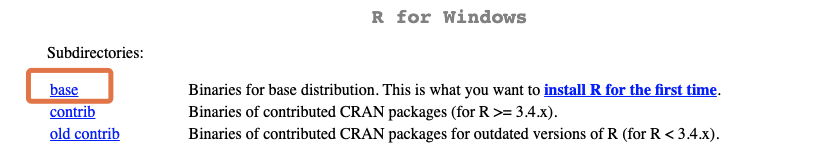
\includegraphics[width=5.91667in,height=\textheight]{images/install_r_windows_base.png}
\item
  Then click on the download link at the top of the page to download the
  latest version of R:

  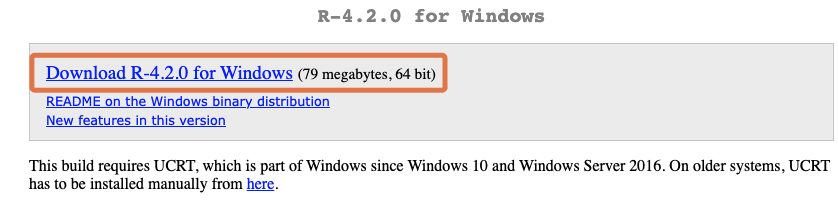
\includegraphics[width=5.92708in,height=\textheight]{images/install_r_windows_download2.png}

  Note that the screenshot above may not show the latest version.
\item
  After the download is finished, click on the downloaded file, then
  follow the instructions on the installation pop-up window. During
  installation, you should not have to change any of the defaults; just
  keep clicking ``Next'' until the installation is done.

  Well done! You should now have R on your computer. But you likely
  won't ever need to interact with R directly. Instead you'll use the
  RStudio IDE to work with R. Follow the instructions in the next
  section to get RStudio.
\end{enumerate}

\hypertarget{download-install-run-rstudio-2}{%
\subsection{Download, install \& run
RStudio}\label{download-install-run-rstudio-2}}

To download RStudio, go to
\href{https://www.rstudio.com/products/rstudio/download/\#download}{rstudio.com/products/rstudio/download/\#download}
and download the Windows version.

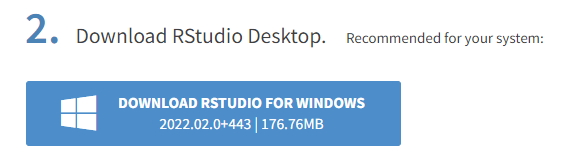
\includegraphics[width=4.16667in,height=\textheight]{images/install_rstudio_button_windows.png}

After the download is finished, click on the downloaded file and follow
the installation instructions.

Once installed, RStudio can be opened like any application on your
computer: press the Windows key to bring up the Start menu, and search
for ``rstudio''. Click to to open the app:

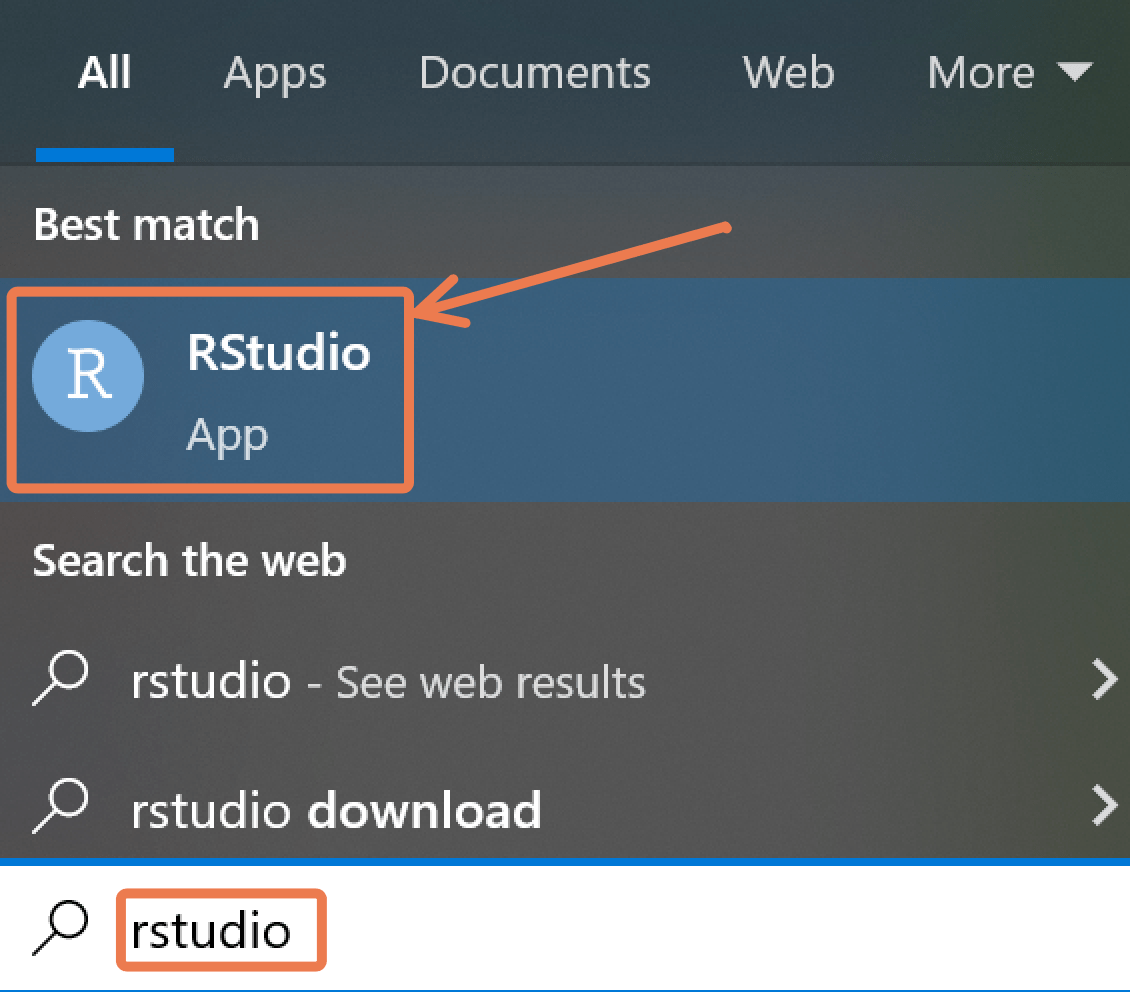
\includegraphics[width=4.16667in,height=\textheight]{images/open_rstudio_windows.png}

You should see a window like this:

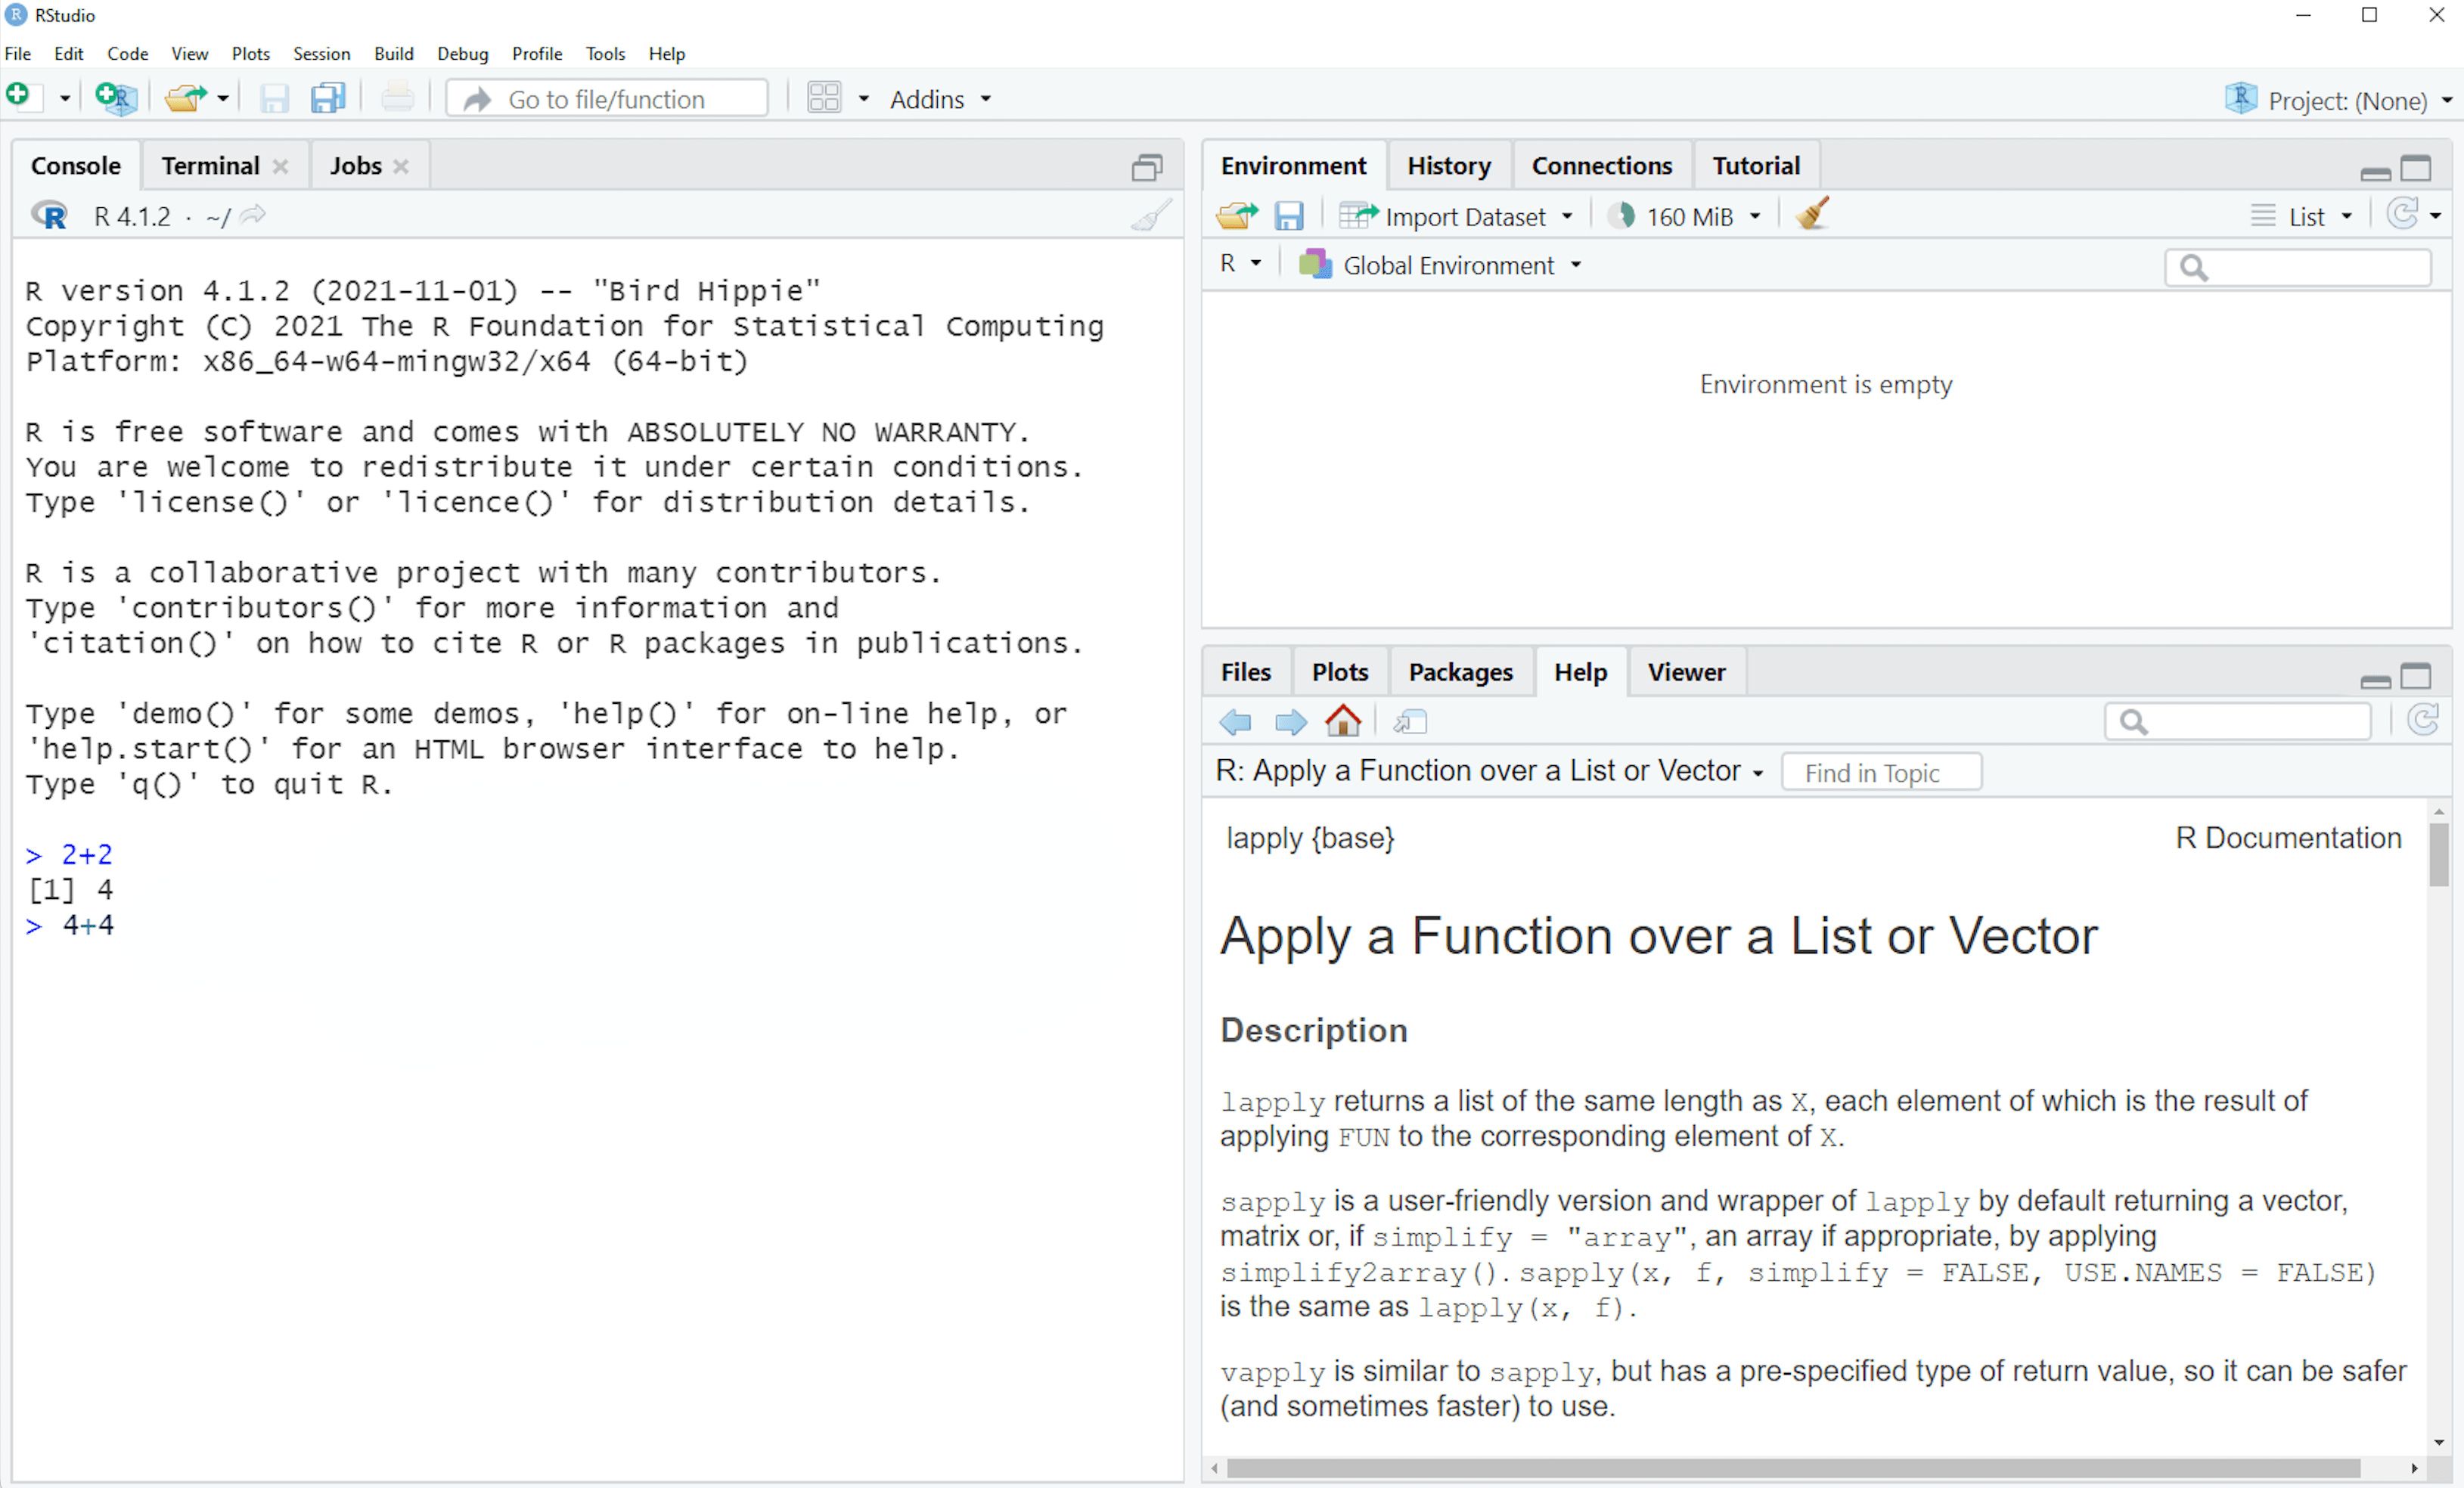
\includegraphics[width=6.1875in,height=\textheight]{images/rstudio_first_view_windows.png}

This is RStudio, your new home for a long time to come!

You can start using R by typing code into the ``console'' pane on the
left:

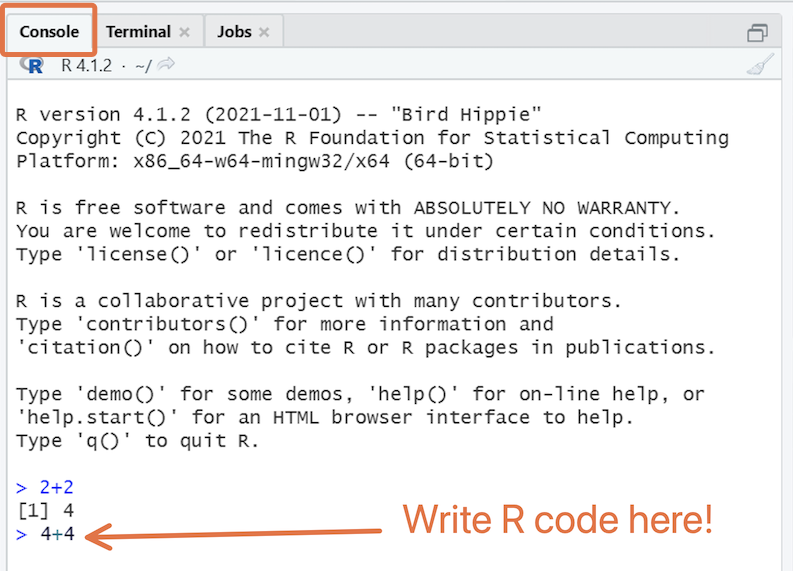
\includegraphics[width=5.20833in,height=\textheight]{images/windows_write_code_here.png}

Try using R as a calculator here; type \texttt{2\ +\ 2} and press Enter.

That's it; you're ready to roll. Proceed to the ``wrapping up'' section
of the lesson.

\hypertarget{set-up-on-macos-1}{%
\section{Set up on macOS}\label{set-up-on-macos-1}}

\hypertarget{download-and-install-r-3}{%
\subsection{Download and install R}\label{download-and-install-r-3}}

If you're working on macOS, follow the steps below to download and
install R:

\begin{enumerate}
\def\labelenumi{\arabic{enumi}.}
\item
  Go to \href{https://cran.rstudio.com/}{cran.rstudio.com} to access the
  R installation page. Then click the link for macOS:

  
\includegraphics[width=4.46875in,height=\textheight]{images/install_r_select_mac.png}
\item
  Download and install the relevant R version for your Mac. For most
  people, the first option under ``Latest release'' will be the one to
  get.

  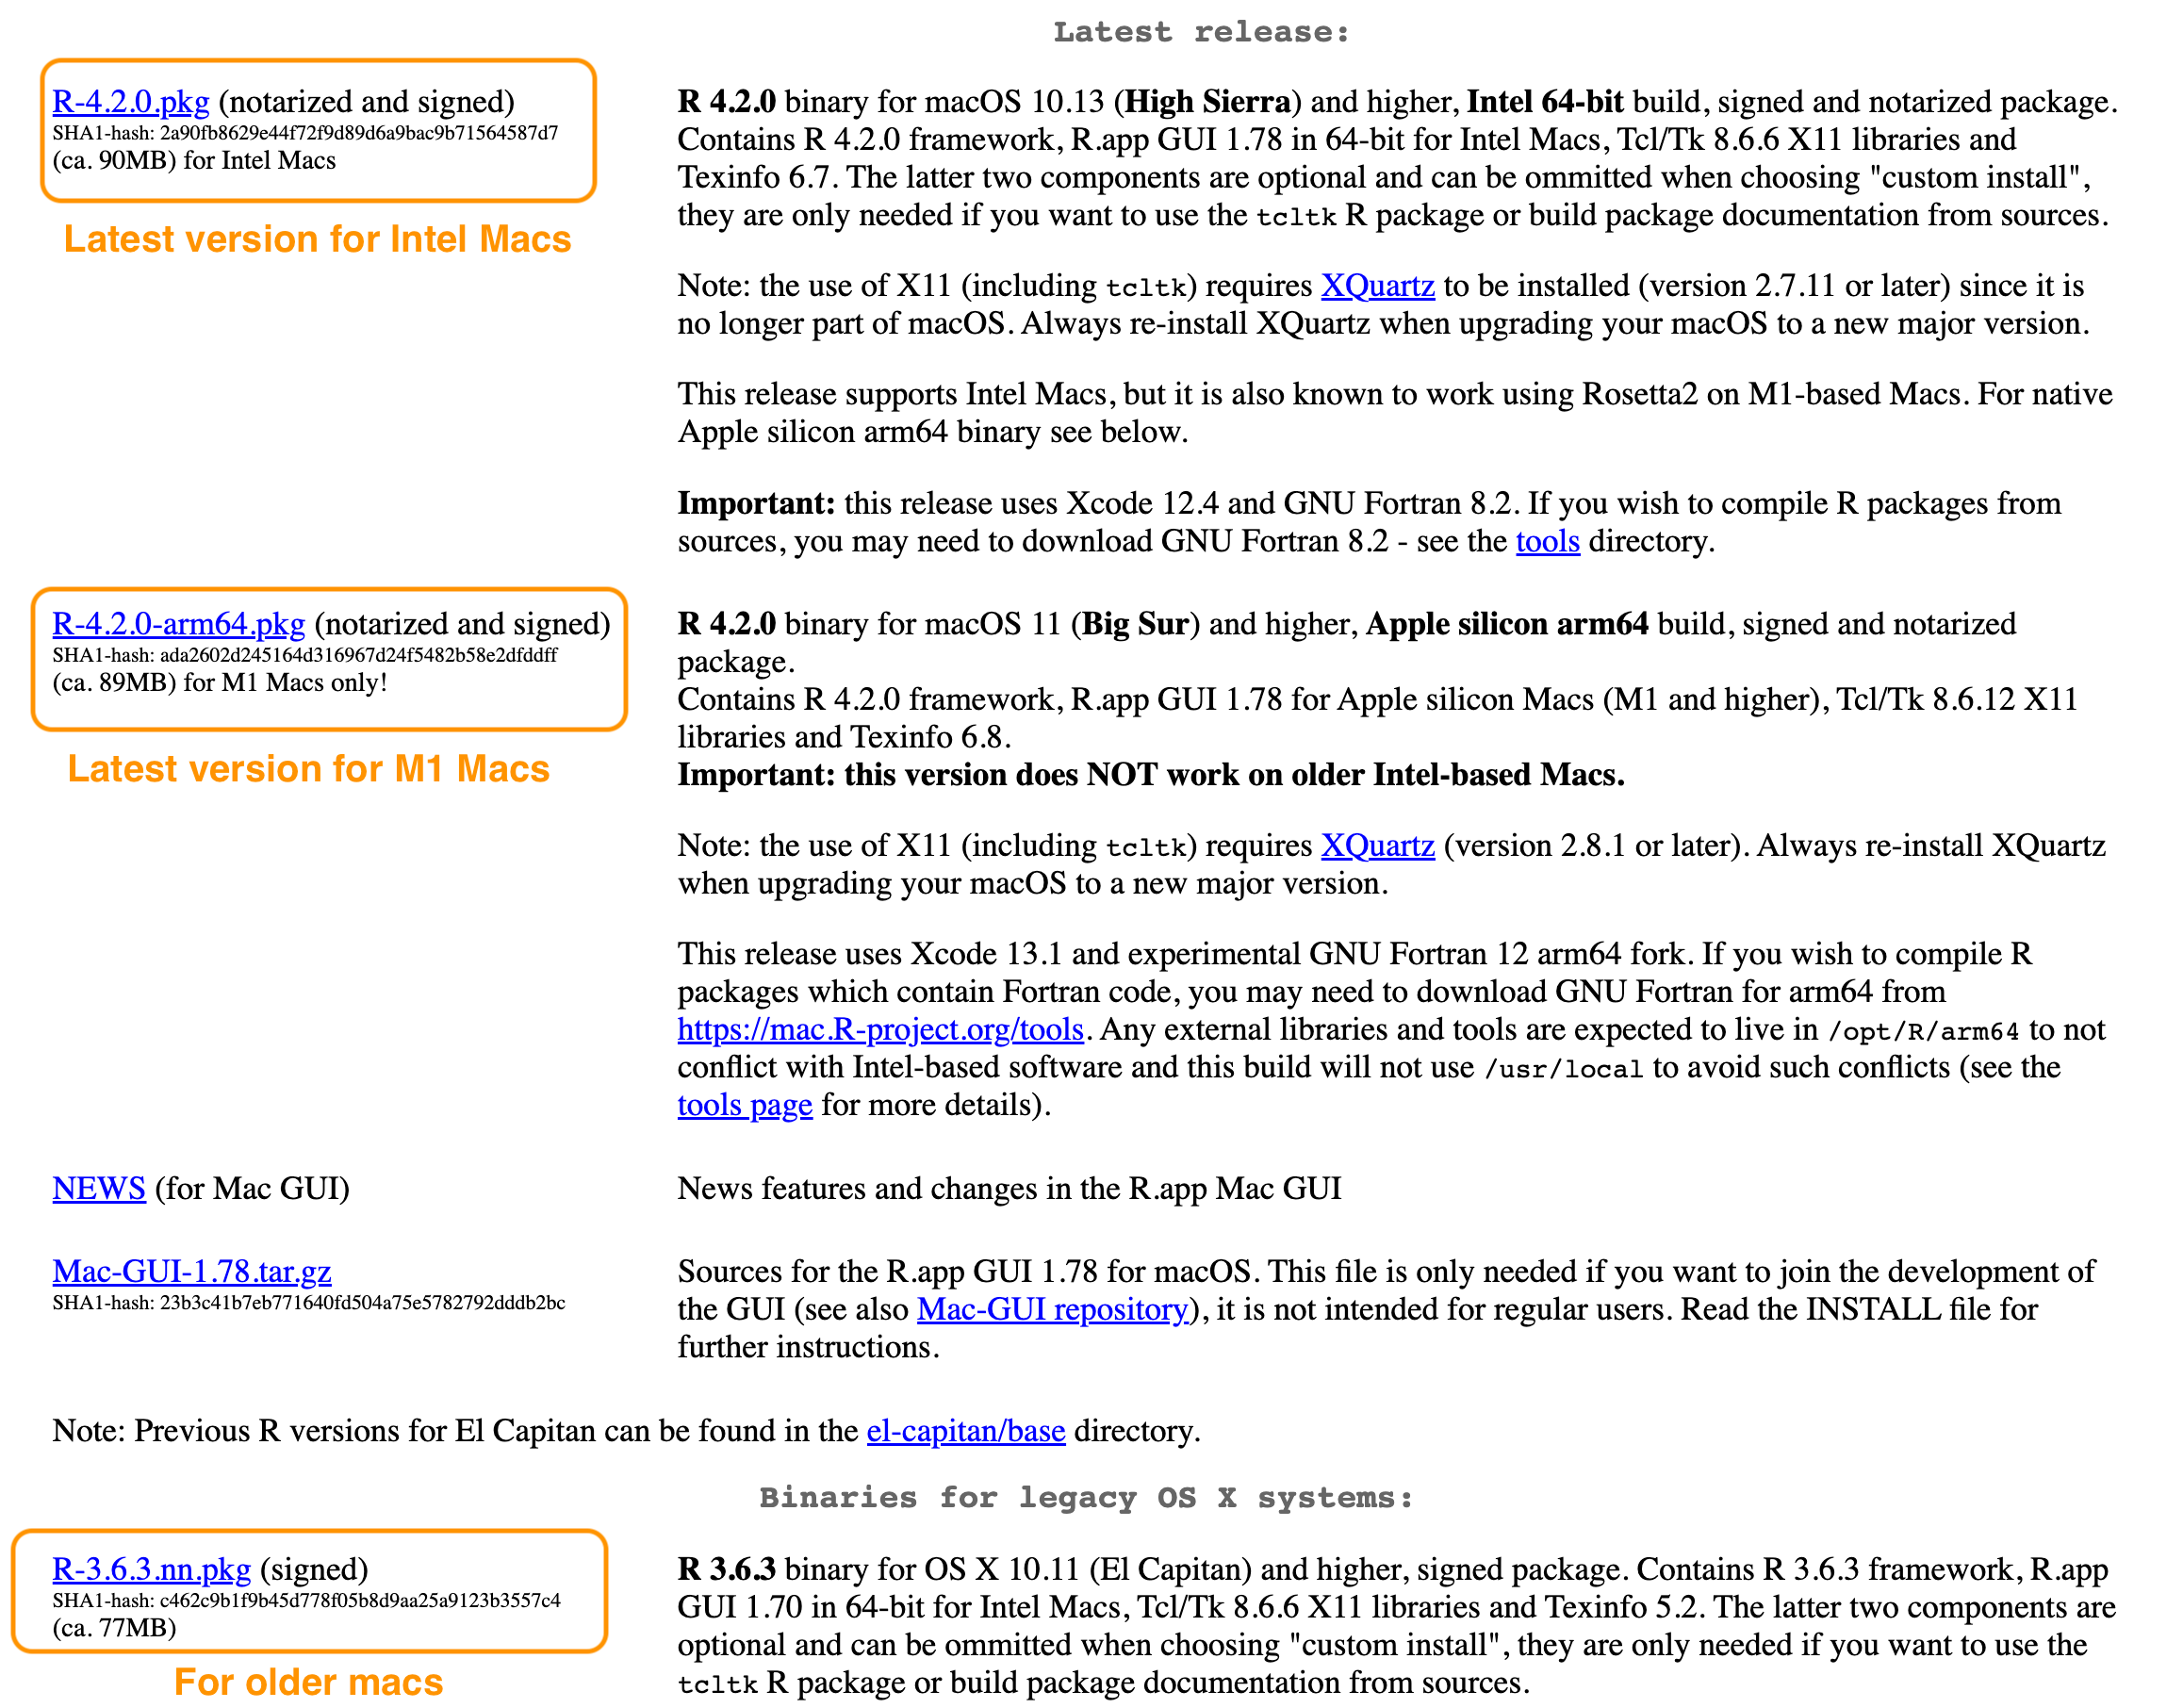
\includegraphics[width=4.39583in,height=\textheight]{images/r_mac_select_version.png}
\item
  After the download is finished, click on the downloaded file, then
  follow the instructions on the installation pop-up window.
\end{enumerate}

Well done! You should now have R on your computer. But you likely won't
ever need to interact with R directly. Instead you'll use the RStudio
IDE to work with R. Follow the instructions in the next section to get
RStudio.

\hypertarget{download-install-run-rstudio-3}{%
\subsection{Download, install \& run
RStudio}\label{download-install-run-rstudio-3}}

To download RStudio, go to
\href{https://www.rstudio.com/products/rstudio/download/\#download}{rstudio.com/products/rstudio/download/\#download}
and download the version for macOS.

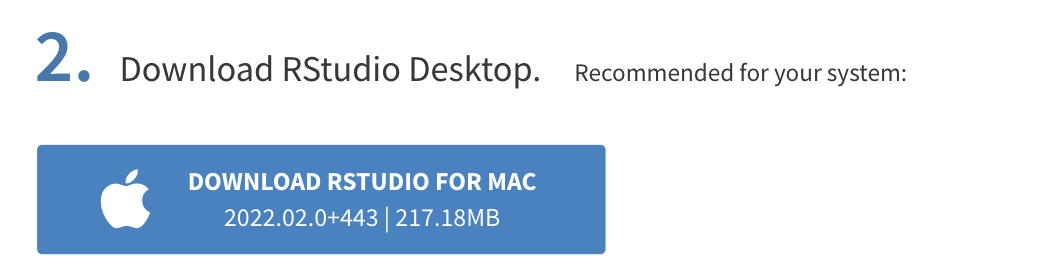
\includegraphics[width=4.16667in,height=\textheight]{images/download_rstudio_button_mac.png}

After the download is finished, click on the downloaded file and follow
the installation instructions.

Once installed, RStudio can be opened like any application on your
computer: Press \texttt{Command} + \texttt{Space} to open Spotlight,
then search for ``rstudio''. Click to open the app.


\includegraphics[width=4.16667in,height=\textheight]{images/mac_spotlight_rstudio.png}

You should see a window like this:

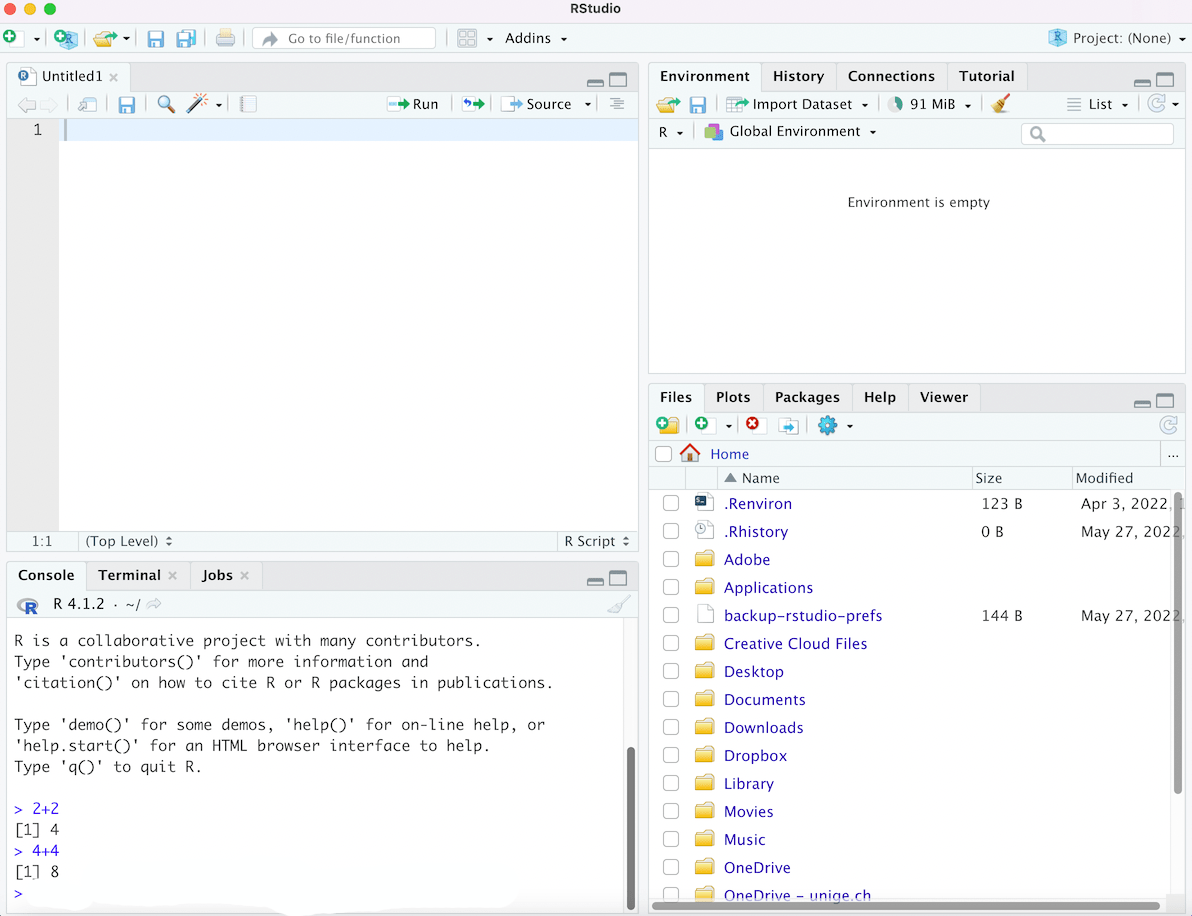
\includegraphics[width=5.375in,height=\textheight]{images/mac_rstudio_window.png}

This is RStudio, your new home for a long time to come!

You can start using R by typing code into the ``console'' pane on the
left:

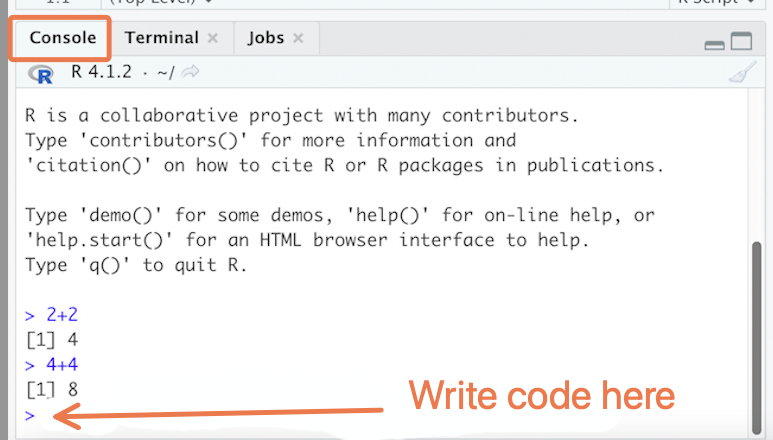
\includegraphics[width=5.20833in,height=\textheight]{images/mac_write_code_here.png}

Try using R as a calculator here; type \texttt{2\ +\ 2} and press Enter.

\hypertarget{wrap-up-1}{%
\section{Wrap up}\label{wrap-up-1}}

You should now have access to R and RStudio, so you're all set to begin
the journey of learning to use these immensely powerful tools. See you
in the next session!

\hypertarget{references-1}{%
\section*{References}\label{references-1}}

\markright{References}

Some material in this lesson was adapted from the following sources:

\begin{itemize}
\tightlist
\item
  Nordmann, Emily, and Heather Cleland-Woods. \emph{Chapter 2
  Programming Basics \textbar{} Data Skills}.
  \emph{psyteachr.github.io},
  \url{https://psyteachr.github.io/data-skills-v1/programming-basics.html}
  Accessed 23 Feb.~2022.
\end{itemize}

\bookmarksetup{startatroot}

\hypertarget{using-rstudio}{%
\chapter{Using RStudio}\label{using-rstudio}}

\begin{center}\rule{0.5\linewidth}{0.5pt}\end{center}

\hypertarget{learning-objectives}{%
\section{Learning objectives}\label{learning-objectives}}

\begin{enumerate}
\def\labelenumi{\arabic{enumi}.}
\item
  You can identify and use the following tabs in RStudio: Source,
  Console, Environment, History, Files, Plots, Packages, Help and
  Viewer.
\item
  You can modify RStudio's interface options to suit your needs.
\end{enumerate}

\hypertarget{introduction-3}{%
\section{Introduction}\label{introduction-3}}

Now that you have access to R \& RStudio, let's go on a quick tour of
the RStudio interface, your digital home for a long time to come.

We will cover a lot of territory quickly. Do not panic. You are not
expected to remember it all this. Rather, you will see these topics
again and again throughout the course, and you will naturally assimilate
them that way.

You can also refer back to this lesson as you progress.

The goal here is simply to make you aware of the tools at your disposal
within RStudio.

\begin{center}\rule{0.5\linewidth}{0.5pt}\end{center}

To get started, you need to open the RStudio application:

\begin{itemize}
\item
  If you are working with RStudio Cloud, go to
  \href{https://rstudio.cloud}{rstudio.cloud}, log in, then click on the
  ``r\_intro'' project that you created in the last lesson. (If you do
  not see this, simply create a new R project using the ``New Project''
  icon at the top right).
\item
  If you are working on your local computer, go to your applications
  folder and double click on the RStudio icon. Or you search for this
  application from your Start Menu (Windows), or through Spotlight
  (Mac).
\end{itemize}

\hypertarget{the-rstudio-panes}{%
\section{The RStudio panes}\label{the-rstudio-panes}}

By default, RStudio is arranged into four window panes.

If you only see three panes, open a new script with
\texttt{File\ \textgreater{}\ New\ File\ \textgreater{}\ R\ Script} .
This should reveal one more pane.


\includegraphics[width=4.69792in,height=0.73958in]{images/new_r_script.jpg}

Before we go any further, we will rearrange these panes to improve the
usability of the interface.

To do this, in the RStudio menu at the top of the screen, select
\texttt{Tools\ \textgreater{}\ Global\ Options} to bring up RStudio's
options. Then under \texttt{Pane\ Layout}, adjust the pane arrangement.
The arrangement we recommend is shown below.

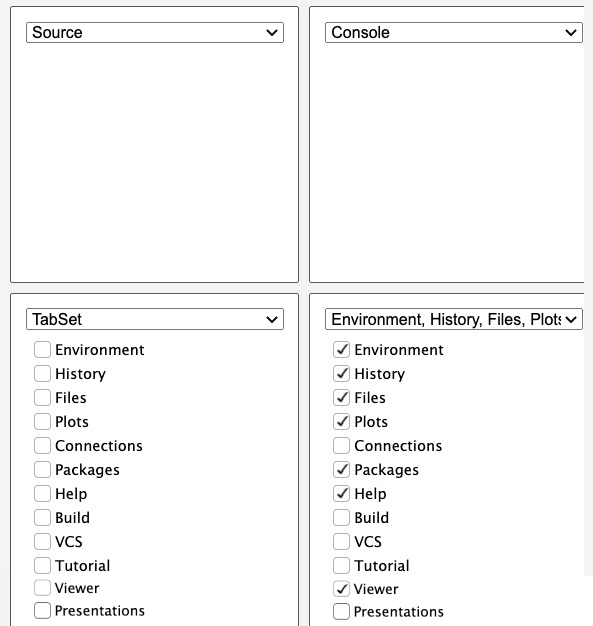
\includegraphics[width=4.19792in,height=\textheight]{images/rstudio_pane_layout.png}

At the top left pane is the Source tab, and at the top right pane, you
should have the Console tab.

Then at the bottom left pane, no tab options should checked---this
section should be left empty, with the drop-down saying just ``TabSet''.

Finally, at the bottom right pane, you should check the following tabs:
Environment, History, Files, Plots, Packages, Help and Viewer.

\begin{center}\rule{0.5\linewidth}{0.5pt}\end{center}

Great, now you should have an RStudio window that looks something like
this:

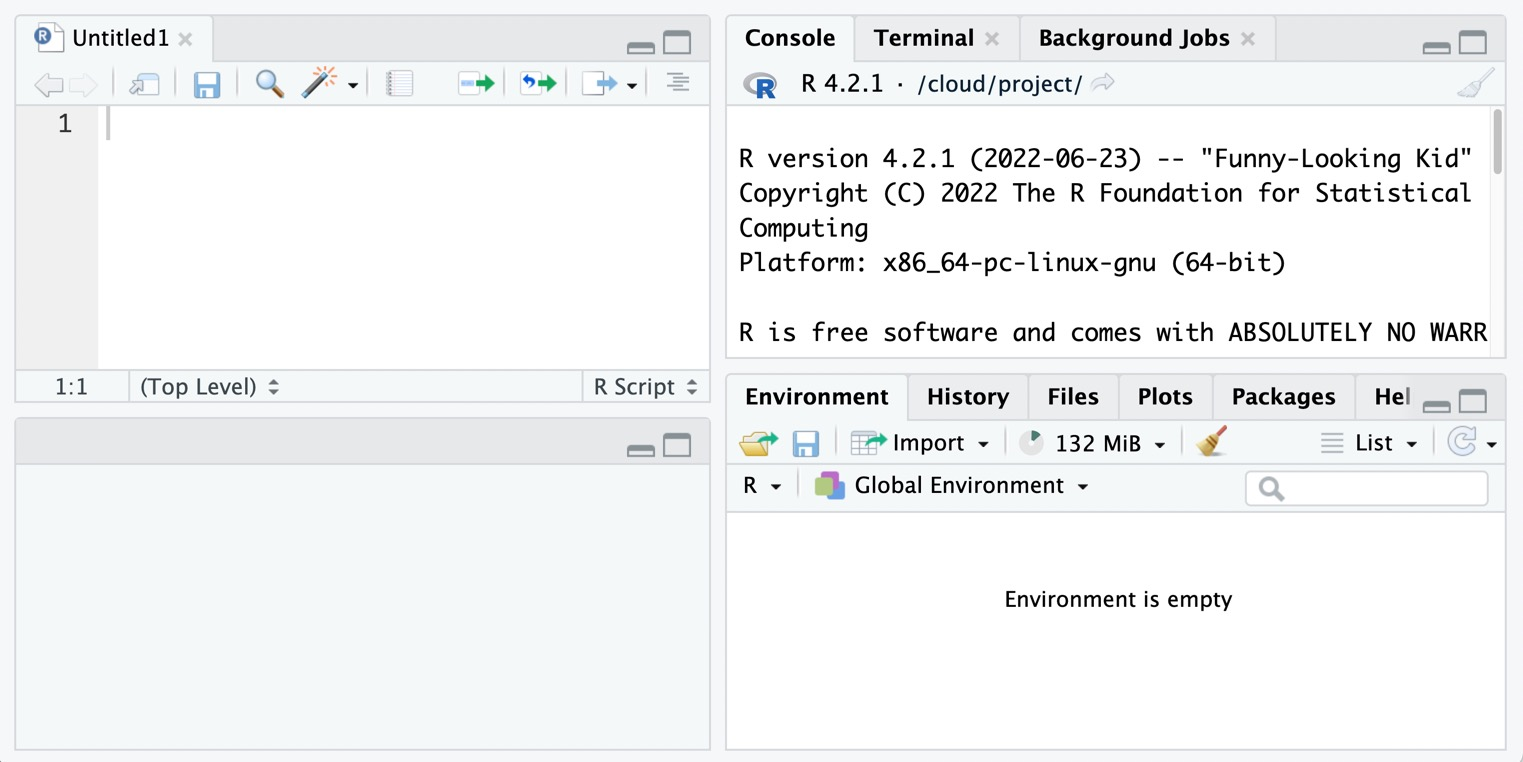
\includegraphics[width=5.08333in,height=\textheight]{images/rstudio_four_panes_rearranged.jpg}

\begin{center}\rule{0.5\linewidth}{0.5pt}\end{center}

The top-left pane is where you will do most of the coding. Make this
larger by clicking on its maximize icon:

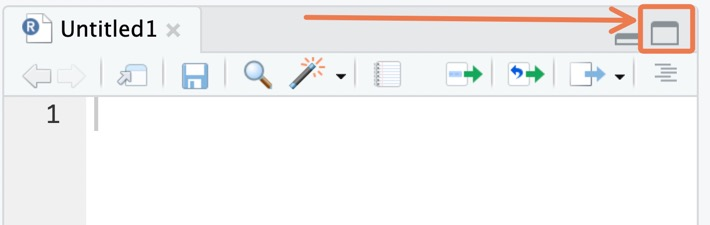
\includegraphics[width=3.67708in,height=\textheight]{images/maximize_icon.jpg}

\begin{center}\rule{0.5\linewidth}{0.5pt}\end{center}

Note that you can drag the bar that separates the window panes to resize
them.

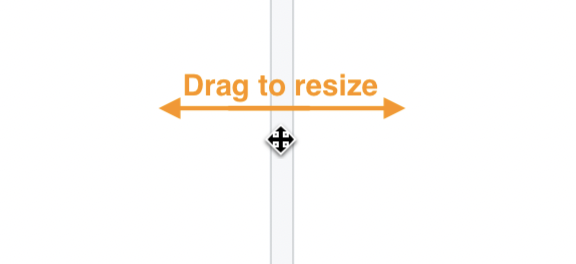
\includegraphics[width=2.40625in,height=\textheight]{images/drag_to_resize_panes.png}

\begin{center}\rule{0.5\linewidth}{0.5pt}\end{center}

Now let's look at each of the RStudio tabs one by one. Below is a
summary image of what we will discuss:

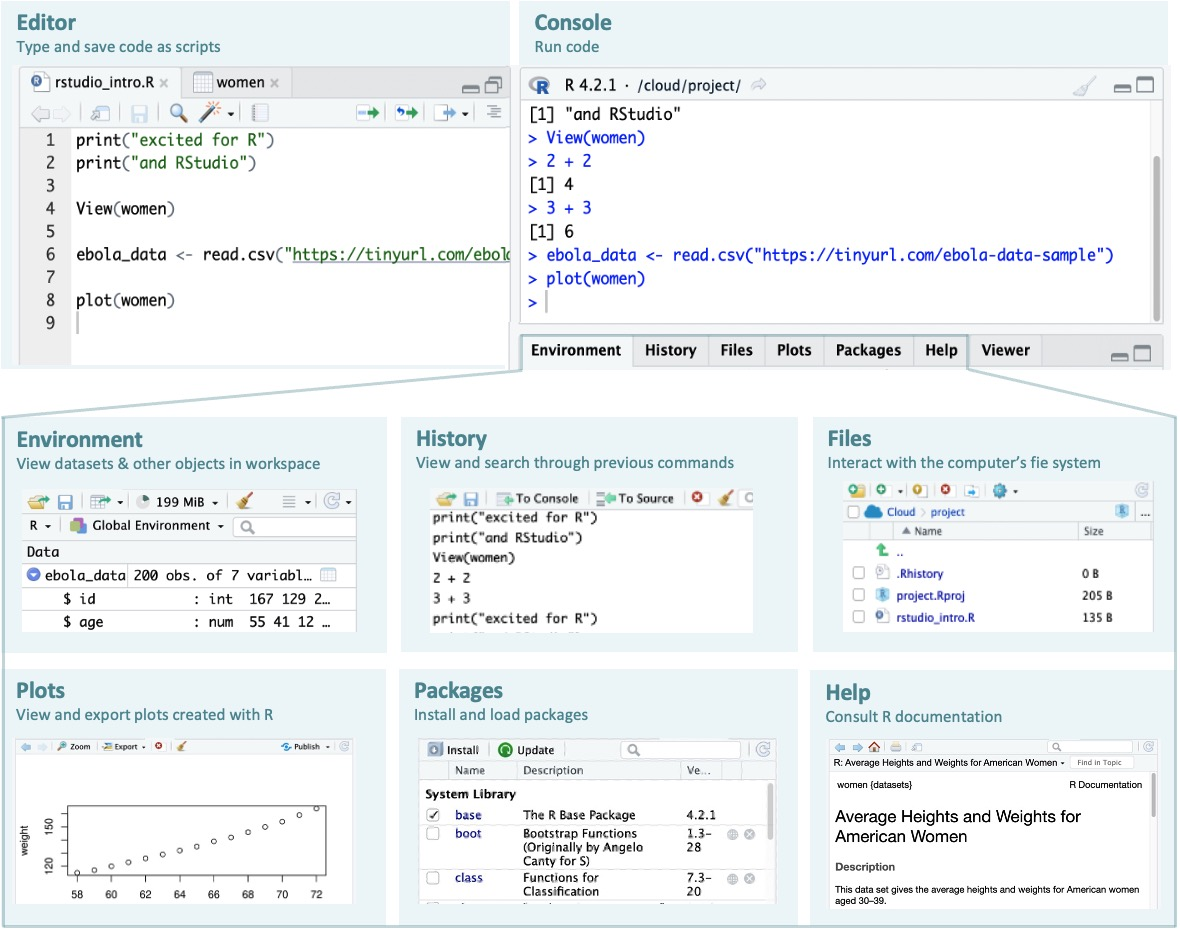
\includegraphics{images/rstudio_panes_detail.jpg}

\hypertarget{sourceeditor}{%
\subsection{Source/Editor}\label{sourceeditor}}

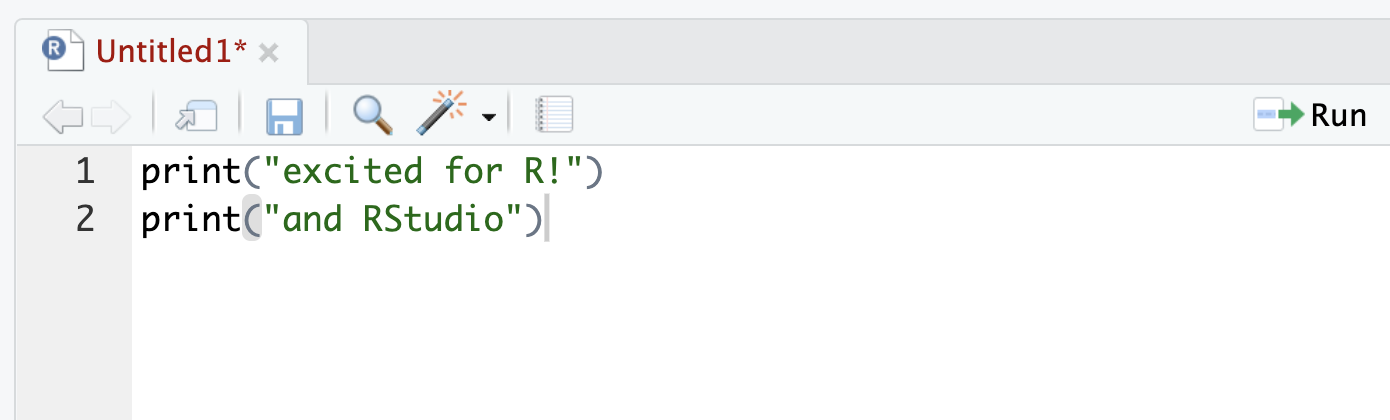
\includegraphics[width=4.88542in,height=\textheight]{images/rstudio_editor.png}

The source or editor is where your R ``scripts'' go. A script is a text
document where you write and save code.

Because this is where you will do most of your coding, it is important
that you have a lot of visual space. That is why we rearranged the
RStudio pane layout above---to give the Editor more space.

Now let's see how to use this Editor.

\begin{center}\rule{0.5\linewidth}{0.5pt}\end{center}

First, \textbf{open a new script} under the File menu if one is not yet
open:
\texttt{File\ \textgreater{}\ New\ File\ \textgreater{}\ R\ Script}. In
the script, type the following:

\begin{Shaded}
\begin{Highlighting}[]
\FunctionTok{print}\NormalTok{(}\StringTok{"excited for R!"}\NormalTok{)}
\end{Highlighting}
\end{Shaded}

To \textbf{run code}, place your cursor anywhere in the code, then hit
\texttt{Command} + \texttt{Enter} on macOS, or \texttt{Control} +
\texttt{Enter} on Windows.

This should send the code to the Console and run it.

\begin{center}\rule{0.5\linewidth}{0.5pt}\end{center}

You can also \textbf{run multiple lines at once}. To try this, add a
second line to your script, so that it now reads:

\begin{Shaded}
\begin{Highlighting}[]
\FunctionTok{print}\NormalTok{(}\StringTok{"excited for R!"}\NormalTok{)}
\FunctionTok{print}\NormalTok{(}\StringTok{"and RStudio!"}\NormalTok{)}
\end{Highlighting}
\end{Shaded}

Now drag your cursor to highlight both lines and press
\texttt{Command}/\texttt{Control} + \texttt{Enter}.

To \textbf{run the entire script}, you can use
\texttt{Command}/\texttt{Control} + \texttt{A} to select all code, then
press \texttt{Command}/\texttt{Control} + \texttt{Enter}. Try this now.
Deselect your code, then try to the shortcut to select all.

\begin{tcolorbox}[enhanced jigsaw, colframe=quarto-callout-note-color-frame, rightrule=.15mm, opacityback=0, breakable, coltitle=black, colbacktitle=quarto-callout-note-color!10!white, bottomrule=.15mm, leftrule=.75mm, toprule=.15mm, arc=.35mm, bottomtitle=1mm, colback=white, left=2mm, opacitybacktitle=0.6, titlerule=0mm, title=\textcolor{quarto-callout-note-color}{\faInfo}\hspace{0.5em}{Side Note}, toptitle=1mm]

There is also a `Run' button at the top right of the source panel (

\includegraphics[width=0.38542in,height=\textheight]{images/run_icon.jpg}
), with which you can run code (either the current line, or all
highlighted code). But you should try to use the keyboard shortcut
instead.

\end{tcolorbox}

\begin{center}\rule{0.5\linewidth}{0.5pt}\end{center}

To \textbf{open the script in a new window}, click on the third icon in
the toolbar directly above the script.

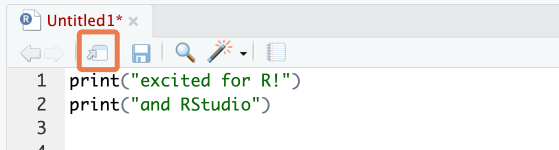
\includegraphics[width=3.42708in,height=\textheight]{images/rstudio_pop_out_icon.png}

To put the window back, click on the same button on the now-external
window.

\begin{center}\rule{0.5\linewidth}{0.5pt}\end{center}

Next, \textbf{save the script.} Hit \texttt{Command}/\texttt{Control} +
\texttt{S} to bring up the Save dialog box. Give it a file name like
``rstudio\_intro''.

\begin{itemize}
\item
  If you are working with RStudio cloud, the file will be saved in your
  project folder.
\item
  If you are working on your local computer, save the file in an
  easy-to-locate part of your computer, perhaps your desktop. (Later on
  we will think about the ``proper'' way to organize and store scripts).
\end{itemize}

\begin{center}\rule{0.5\linewidth}{0.5pt}\end{center}

You can \textbf{view data frames} (which are like spreadsheets in R) in
the same pane. To observe this, type and run the code below on a new
line in your script:

\begin{Shaded}
\begin{Highlighting}[]
\FunctionTok{View}\NormalTok{(women)}
\end{Highlighting}
\end{Shaded}

Notice the uppercase ``V'' in \texttt{View()}.

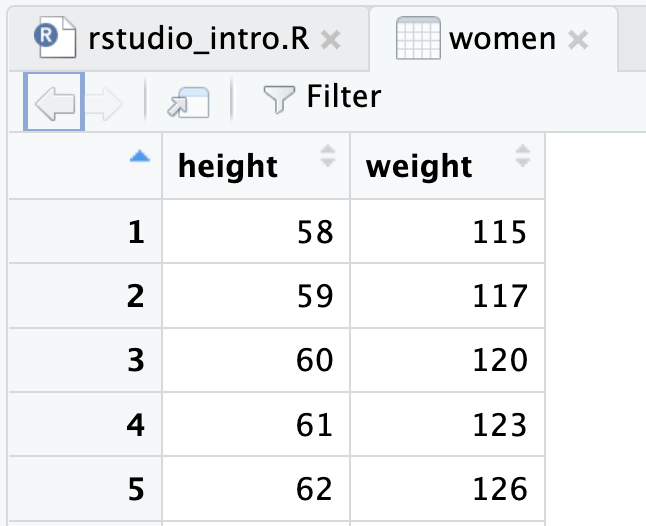
\includegraphics[width=2.4375in,height=\textheight]{images/rstudio_view_data_frame.png}

\texttt{women} is the name of a dataset that comes loaded with R. It
gives the average heights and weights for American women aged 30--39.

You can click on the ``x'' icon to the right of the ``women'' tab to
close this data viewer.

\begin{center}\rule{0.5\linewidth}{0.5pt}\end{center}

\hypertarget{console}{%
\subsection{Console}\label{console}}

The \emph{console}, at the bottom left, is where \textbf{code is
executed}. You can type code directly here, but it will not be saved.

Type a random piece of code (maybe a calculation like \texttt{3\ +\ 3})
and press `Enter'.

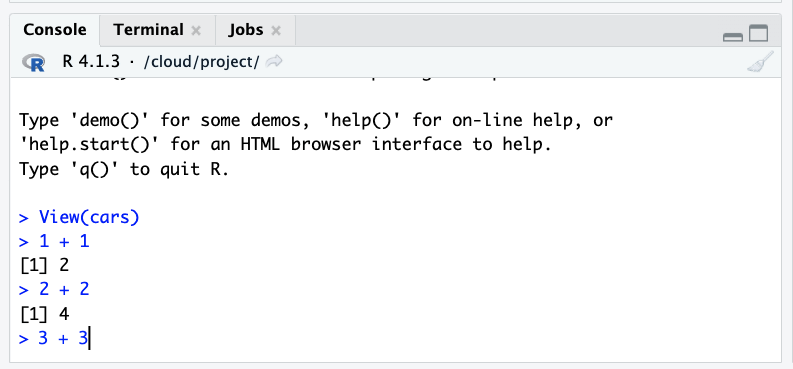
\includegraphics[width=6.1875in,height=\textheight]{images/rstudio_console.png}

If you place your cursor on the last line of the console, and you press
the \textbf{up arrow}, you can go back to the last code that was run.
Keep pressing it to cycle to the previous lines.

To run any of these previous lines, press \emph{Enter}.

\hypertarget{environment}{%
\subsection{Environment}\label{environment}}

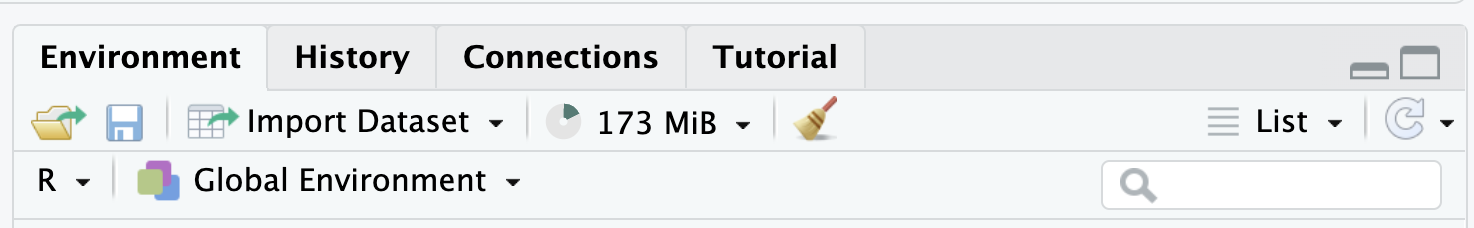
\includegraphics[width=5.48958in,height=\textheight]{images/environment_tab.png}

At the top right of the RStudio Window, you should see the
\textbf{Environment} tab.

The Environment tab shows datasets and other objects that are loaded
into R's working memory, or ``workspace''.

To explore this tab, let's import a dataset into your environment from
the web. Type the code below into your script and run it:

\begin{Shaded}
\begin{Highlighting}[]
\NormalTok{ebola\_data }\OtherTok{\textless{}{-}} \FunctionTok{read.csv}\NormalTok{(}\StringTok{"https://tinyurl.com/ebola{-}data{-}sample"}\NormalTok{)}
\end{Highlighting}
\end{Shaded}

\begin{tcolorbox}[enhanced jigsaw, colframe=quarto-callout-note-color-frame, rightrule=.15mm, opacityback=0, breakable, coltitle=black, colbacktitle=quarto-callout-note-color!10!white, bottomrule=.15mm, leftrule=.75mm, toprule=.15mm, arc=.35mm, bottomtitle=1mm, colback=white, left=2mm, opacitybacktitle=0.6, titlerule=0mm, title=\textcolor{quarto-callout-note-color}{\faInfo}\hspace{0.5em}{Side Note}, toptitle=1mm]

You don't need to understand exactly what the code above is doing for
now. We just want to quickly show you the basic features of the
Environment pane; we'll look at data importing in detail later.

Also, if you do not have active internet access, the code above will not
run. You can skip this section and move to the ``History'' tab.

\end{tcolorbox}

You have now imported the dataset and stored it in an \emph{object}
named \texttt{ebola\_data}. (You could have named the object anything
you want.)

Now that the dataset is stored by R, you should be able to see it in the
Environment pane. If you click on the blue drop-down icon beside the
object's name in the Environment tab to reveal a summary.

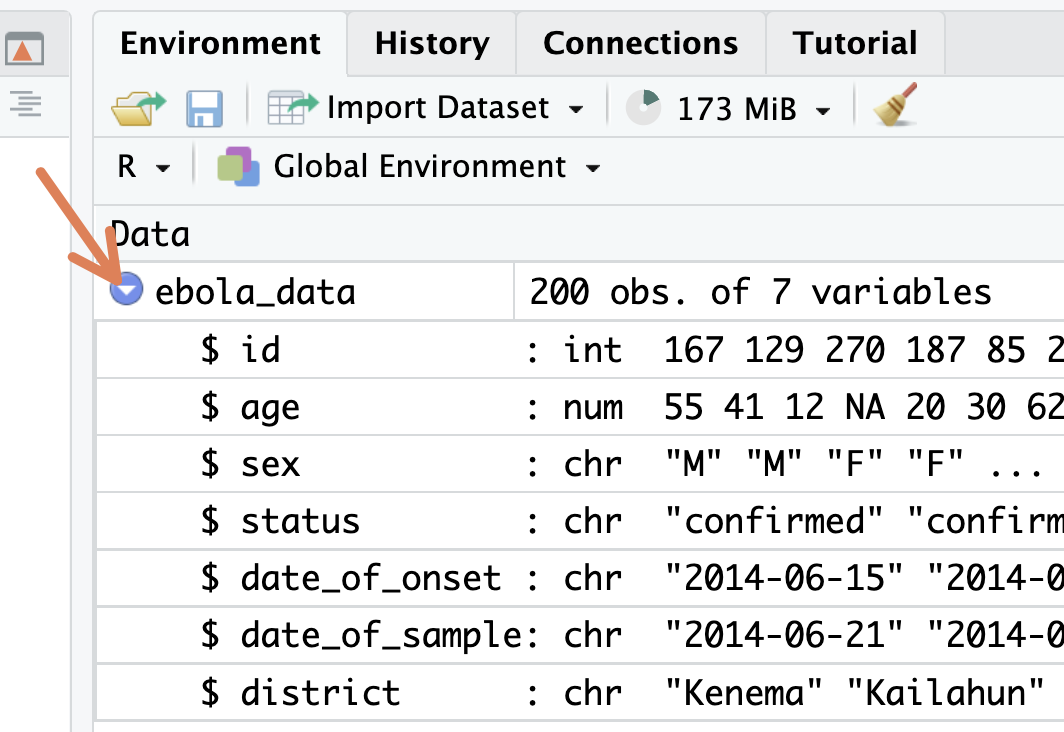
\includegraphics[width=3.65625in,height=\textheight]{images/rstudio_explore_object_dropdown.png}

Try clicking directly on the \texttt{ebola\_data} dataset from the
Environment tab. This opens it in a `View' tab.

\begin{center}\rule{0.5\linewidth}{0.5pt}\end{center}

You can \textbf{remove an object from the workspace} with the
\texttt{rm()} function. Type and run the following in a new line on your
R script.

\begin{Shaded}
\begin{Highlighting}[]
\FunctionTok{rm}\NormalTok{(ebola\_data)}
\end{Highlighting}
\end{Shaded}

Notice that the \texttt{ebola\_data} object no longer shows up in your
environment after having run that code.

The broom icon, at the top of the Environment pane can also be used to
clear your workspace.

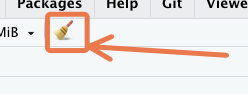
\includegraphics{images/broom_icon.png}

To practice using it, try re-running the line above that imports the
Ebola dataset, then clear the object using the broom icon.

\hypertarget{history}{%
\subsection{History}\label{history}}

Next, the \textbf{History} tab shows previous commands you have run.

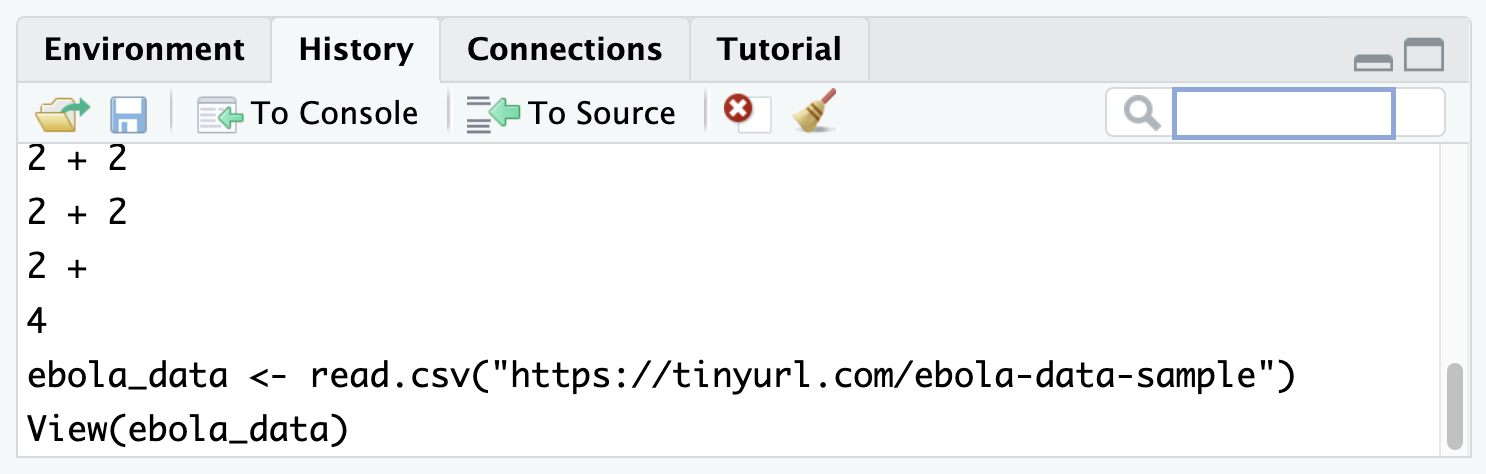
\includegraphics[width=4.89583in,height=\textheight]{images/history_tab.png}

You can click a line to highlight it, then send it to the console or to
your script with the ``To Console'' and ``To Source'' icons at the top
of this tab.

To select multiple lines, use the ``Shift-click'' method: click the
first item you want to select, then hold down the ``Shift'' key and
click the last item you want to select.

Finally, notice that there is a search bar at the top right of the
History pane where you can search for past commands that you have run.

\hypertarget{files}{%
\subsection{Files}\label{files}}

Next, the \textbf{Files} tab. This shows the files and folders in the
folder you are working in.

\includegraphics{images/rstudio_files.png}

The tab allows you to interact with your computer's file system.

Try playing with some of the buttons here, to see what they do. You
should try at least the following:

\begin{itemize}
\item
  Make a new folder
\item
  Delete that folder
\item
  Make a new R Script
\item
  Rename that script
\end{itemize}

\hypertarget{plots}{%
\subsection{Plots}\label{plots}}

Next, the \textbf{Plots} tab. This is where figures that are generated
by R will show up. Try creating a simple plot with the following code:

\begin{Shaded}
\begin{Highlighting}[]
\FunctionTok{plot}\NormalTok{(women)}
\end{Highlighting}
\end{Shaded}

\includegraphics{images/rstudio_plots.png}

That code creates a plot of the two variables in the \texttt{women}
dataset. You should see this figure in the Plots tab.

Now, test out the buttons at the top of this tab to explore what they
do. In particular, try to export a plot to your computer.

\hypertarget{packages}{%
\subsection{Packages}\label{packages}}

Next, let's look at the \textbf{Packages} tab.

\includegraphics[width=4.36458in,height=\textheight]{images/packages_tab.png}

Packages are collections of R code that extend the functionality of R.
We will discuss packages in detail in a future lesson.

For now, it is important to know that to use a package, you need to
\emph{install} then \emph{load} it. Packages need to be installed only
once, but must be loaded in each new R session.

All the package names you see (in blue font) are packages that are
installed on your system. And packages with a checkmark are packages
which are \emph{loaded} in the current session.

You can install a package with the Install button of the Packages tab.

\includegraphics[width=3.625in,height=\textheight]{images/rstudio_install_package_icon.png}

But it is better to install and load packages with R code, rather than
the Install button. Let's try this. Type and run the code below to
install the \{highcharter\} package.

\begin{Shaded}
\begin{Highlighting}[]
\FunctionTok{install.packages}\NormalTok{(}\StringTok{"highcharter"}\NormalTok{)}
\FunctionTok{library}\NormalTok{(highcharter)}
\end{Highlighting}
\end{Shaded}

The first line installs the package. The second line \emph{loads} the
package from your package library.

Because you only need to install a package once, you can now remove the
installation line from your script.

\begin{center}\rule{0.5\linewidth}{0.5pt}\end{center}

Now that the \{highcharter\} package has been installed and loaded, you
can use the functions that come in the package. To try this, type and
run the code below:

\begin{Shaded}
\begin{Highlighting}[]
\NormalTok{highcharter}\SpecialCharTok{::}\FunctionTok{hchart}\NormalTok{(women}\SpecialCharTok{$}\NormalTok{weight)}
\end{Highlighting}
\end{Shaded}

\begin{verbatim}
Registered S3 method overwritten by 'quantmod':
  method            from
  as.zoo.data.frame zoo 
\end{verbatim}

\begin{figure}[H]

{\centering \includegraphics{foundations_ls02_using_rstudio_files/figure-pdf/unnamed-chunk-9-1.pdf}

}

\end{figure}

This code uses the \texttt{hchart()} \emph{function} from the
\{highcharter\} package to plot an interactive histogram showing the
distribution of weights in the \texttt{women} dataset.

(Of course, you may not yet know what a function is. We'll get to this
soon.)

\hypertarget{viewer}{%
\subsection{Viewer}\label{viewer}}

Notice that the histogram above shows up in a \textbf{Viewer} tab. This
tab allows you to preview HTML files and interactive objects.

\hypertarget{help}{%
\subsection{Help}\label{help}}

Lastly, the \textbf{Help} tab shows the documentation for different R
objects. Try typing out and running each line below to see what this
documentation looks like.

\begin{Shaded}
\begin{Highlighting}[]
\NormalTok{?hchart}
\NormalTok{?women}
\NormalTok{?read.csv}
\end{Highlighting}
\end{Shaded}

\includegraphics[width=4.69792in,height=\textheight]{images/example_help_page.png}

Help files are not always very easy to understand for beginners, but
with time they will become more useful.

\hypertarget{rstudio-options}{%
\section{RStudio options}\label{rstudio-options}}

RStudio has a number of useful options for changing it's look and
functionality. Let's try these. You may not understand all the changes
made for now. That's fine.

In the RStudio menu at the top of the screen, select
\texttt{Tools\ \textgreater{}\ Global\ Options} to bring up RStudio's
options.

\begin{itemize}
\item
  Now, under \texttt{Appearance}, choose your ideal theme. (We like the
  ``Crimson Editor'' and ``Tomorrow Night'' themes.)

  \includegraphics[width=5.52083in,height=\textheight]{images/rstudio_themes.png}
\item
  Under \texttt{Code\ \textgreater{}\ Display}, check ``Highlight R
  function calls''. What this does is give your R \emph{functions} a
  unique color, improving readability. You will understand this later.
\item
  Also under \texttt{Code\ \textgreater{}\ Display}, check ``Rainbow
  parentheses''. What this does is make your ``nested parentheses''
  easier to read by giving each pair a unique color.

  \includegraphics[width=4.64583in,height=\textheight]{images/options_highlight_function_rainbow_parentheses.jpg}

  \includegraphics[width=4.79167in,height=0.6875in]{images/highlight_r_function_calls.jpg}

  \includegraphics[width=3.76042in,height=\textheight]{images/rainbow_parentheses.jpg}
\item
  Finally under \texttt{General\ \textgreater{}\ Basic},
  \textbf{uncheck} the box that says \textbf{``Restore .RData into
  workspace at startup''}. You don't want to restore any data to your
  workspace (or \emph{environment)} when you start RStudio. Starting
  with a clean workspace each time is less likely to lead to errors.

  This also means that you never want to \textbf{``save your workspace
  to .RData on exit''}, so set this to \textbf{Never}.
\end{itemize}

\hypertarget{command-palette}{%
\section{Command palette}\label{command-palette}}

The Rstudio command palette gives instant, searchable access to many of
the RStudio menu options and settings that we have seen so far.

The palette can be invoked with the keyboard shortcut \texttt{Ctrl} +
\texttt{Shift} + \texttt{P} (\texttt{Cmd} + \texttt{Shift} + \texttt{P}
on macOS).

It's also available on the \emph{Tools} menu (\emph{Tools}
-\textgreater{} \emph{Show Command Palette}).

\includegraphics[width=5.48958in,height=\textheight]{images/command_palette.jpg}

Try using it to:

\begin{itemize}
\item
  Create a new script (Search ``new script'' and click on the relevant
  option)
\item
  Rename a script (Search ``rename'' and click on the relevant option)
\end{itemize}

\hypertarget{wrapping-up}{%
\section{Wrapping up}\label{wrapping-up}}

Congratulations! You are now a new citizen of RStudio.

Of course, you have only scratched the surface of RStudio functionality.
As you advance in your R journey, you will discover new features, and
you will hopefully grow to love the wonderful integrated development
environment (IDE) that is RStudio. One good place to start is the
official RStudio IDE
\href{https://thegraphcourses.org/wp-content/uploads/2022/03/rstudio-IDE-cheatsheet.pdf}{cheatsheet}.

Below is one section of that sheet:

\includegraphics{images/rstudio_cheatsheet.png}

See you in the next lesson!

\hypertarget{further-resources}{%
\section{Further resources}\label{further-resources}}

\begin{enumerate}
\def\labelenumi{\arabic{enumi}.}
\tightlist
\item
  \href{https://www.dataquest.io/blog/rstudio-tips-tricks-shortcuts/}{23
  RStudio Tips, Tricks, and Shortcuts}
\end{enumerate}

\hypertarget{references-2}{%
\section{References}\label{references-2}}

Some material in this lesson was adapted from the following sources:

\begin{itemize}
\tightlist
\item
  ``Rstudio Cheatsheets.'' \emph{RStudio},
  \url{https://www.rstudio.com/resources/cheatsheets/.}
\item
  ``Chapter 1 Getting Started: Data Skills for Reproducible Research.''
  \emph{Chapter 1 Getting Started \textbar{} Data Skills for
  Reproducible Research},
  \url{https://psyteachr.github.io/reprores-v2/intro.html.}
\end{itemize}

\bookmarksetup{startatroot}

\hypertarget{coding-basics}{%
\chapter{Coding basics}\label{coding-basics}}

\begin{center}\rule{0.5\linewidth}{0.5pt}\end{center}

\hypertarget{learning-objectives-1}{%
\section*{Learning objectives}\label{learning-objectives-1}}

\markright{Learning objectives}

\begin{enumerate}
\def\labelenumi{\arabic{enumi}.}
\item
  You can write comments in R.
\item
  You can create section headers in RStudio.
\item
  You know how to use R as a calculator.
\item
  You can create, overwrite and manipulate R objects.
\item
  You understand the basic rules for naming R objects.
\item
  You understand the syntax for calling R functions.
\item
  You know how to nest multiple functions.
\item
  You can use install and load add-on R packages and call functions from
  these packages.
\end{enumerate}

\hypertarget{introduction-4}{%
\section{Introduction}\label{introduction-4}}

In the last lesson, you learned how to use RStudio, the wonderful
integrated development environment (IDE) that makes working with R much
easier. In this lesson, you will learn the basics of using R itself.

To get started, open RStudio, and open a new script with
\texttt{File\ \textgreater{}\ New\ File\ \textgreater{}\ R\ Script} on
the RStudio menu.

\includegraphics[width=4.69792in,height=0.73958in]{images/new_r_script.jpg}

Next, \textbf{save the script} with \texttt{File\ \textgreater{}\ Save}
on the RStudio menu or by using the shortcut
\texttt{Command}/\texttt{Control} + \texttt{S} . This should bring up
the Save File dialog box. Save the file with a name like
``coding\_basics''.

You should now type all the code from this lesson into that script.

\hypertarget{comments}{%
\section{Comments}\label{comments}}

There are two main types of text in an R script: commands and comments.
A command is a line or lines of R code that instructs R to do something
(e.g.~\texttt{2\ +\ 2})

A comment is text that is ignored by the computer.

Anything that follows a \texttt{\#} symbol (pronounced ``hash'' or
``pound'') on a given line is a comment. Try typing out and running the
code below to see this:

\begin{Shaded}
\begin{Highlighting}[]
\DocumentationTok{\#\# A comment}
\DecValTok{2} \SpecialCharTok{+} \DecValTok{2} \CommentTok{\# Another comment}
\DocumentationTok{\#\# 2 + 2}
\end{Highlighting}
\end{Shaded}

Since they are ignored by the computer, comments are meant for
\emph{humans.} They help you and others keep track of what your code is
doing. Use them often! Like your mother always says, ``too much
everything is bad, except for R comments''.

\begin{tcolorbox}[enhanced jigsaw, colframe=quarto-callout-tip-color-frame, rightrule=.15mm, opacityback=0, breakable, coltitle=black, colbacktitle=quarto-callout-tip-color!10!white, bottomrule=.15mm, leftrule=.75mm, toprule=.15mm, arc=.35mm, bottomtitle=1mm, colback=white, left=2mm, opacitybacktitle=0.6, titlerule=0mm, title=\textcolor{quarto-callout-tip-color}{\faLightbulb}\hspace{0.5em}{Practice}, toptitle=1mm]

\textbf{Question 1}

True or False: both code chunks below are valid ways to comment code:?

\begin{Shaded}
\begin{Highlighting}[]
\DocumentationTok{\#\# add two numbers}
\DecValTok{2} \SpecialCharTok{+} \DecValTok{2}
\end{Highlighting}
\end{Shaded}

\begin{Shaded}
\begin{Highlighting}[]
\DecValTok{2} \SpecialCharTok{+} \DecValTok{2} \CommentTok{\# add two numbers}
\end{Highlighting}
\end{Shaded}

\textbf{Note:} All question answers can be found at the end of the
lesson.

\end{tcolorbox}

A fantastic use of comments is to separate your scripts into sections.
If you put four dashes after a comment, RStudio will create a new
section in your code:

\begin{Shaded}
\begin{Highlighting}[]
\DocumentationTok{\#\# New section {-}{-}{-}{-}}
\end{Highlighting}
\end{Shaded}

This has two nice benefits. Firstly, you can click on the little arrow
beside the section header to fold, or collapse, that section of code:

\includegraphics[width=1.78125in,height=\textheight]{images/section_folder_icon.jpg}

Second, you can click on the ``Outline'' icon at the top right of the
Editor to view and navigate through all the contents in your script:

\includegraphics[width=2.02083in,height=\textheight]{images/rstudio_outline.jpg}

\hypertarget{r-s-a-calculator}{%
\section{R s a calculator}\label{r-s-a-calculator}}

R works as a calculator, and obeys the correct order of operations. Type
and run the following expressions and observe their output:

\begin{Shaded}
\begin{Highlighting}[]
\DecValTok{2} \SpecialCharTok{+} \DecValTok{2}
\end{Highlighting}
\end{Shaded}

\begin{verbatim}
[1] 4
\end{verbatim}

\begin{Shaded}
\begin{Highlighting}[]
\DecValTok{2} \SpecialCharTok{{-}} \DecValTok{2}
\end{Highlighting}
\end{Shaded}

\begin{verbatim}
[1] 0
\end{verbatim}

\begin{Shaded}
\begin{Highlighting}[]
\DecValTok{2} \SpecialCharTok{*} \DecValTok{2} \CommentTok{\# two times two }
\end{Highlighting}
\end{Shaded}

\begin{verbatim}
[1] 4
\end{verbatim}

\begin{Shaded}
\begin{Highlighting}[]
\DecValTok{2} \SpecialCharTok{/} \DecValTok{2} \CommentTok{\# two divided by two}
\end{Highlighting}
\end{Shaded}

\begin{verbatim}
[1] 1
\end{verbatim}

\begin{Shaded}
\begin{Highlighting}[]
\DecValTok{2} \SpecialCharTok{\^{}} \DecValTok{2} \CommentTok{\# two raised to the power of two}
\end{Highlighting}
\end{Shaded}

\begin{verbatim}
[1] 4
\end{verbatim}

\begin{Shaded}
\begin{Highlighting}[]
\DecValTok{2} \SpecialCharTok{+} \DecValTok{2} \SpecialCharTok{*} \DecValTok{2}   \CommentTok{\# this is evaluated following the order of operations}
\end{Highlighting}
\end{Shaded}

\begin{verbatim}
[1] 6
\end{verbatim}

\begin{Shaded}
\begin{Highlighting}[]
\FunctionTok{sqrt}\NormalTok{(}\DecValTok{100}\NormalTok{)   }\CommentTok{\# square root}
\end{Highlighting}
\end{Shaded}

\begin{verbatim}
[1] 10
\end{verbatim}

The square root command shown on the last line is a good example of an R
\emph{function}, where \texttt{100} is the \emph{argument} to the
function. You will see more functions soon.

\begin{tcolorbox}[enhanced jigsaw, colframe=quarto-callout-note-color-frame, rightrule=.15mm, opacityback=0, breakable, coltitle=black, colbacktitle=quarto-callout-note-color!10!white, bottomrule=.15mm, leftrule=.75mm, toprule=.15mm, arc=.35mm, bottomtitle=1mm, colback=white, left=2mm, opacitybacktitle=0.6, titlerule=0mm, title=\textcolor{quarto-callout-note-color}{\faInfo}\hspace{0.5em}{Reminder}, toptitle=1mm]

We hope you remember the shortcut to run code!

To \textbf{run a single line of code}, place your cursor anywhere on
that line, then hit \texttt{Command} + \texttt{Enter} on macOS, or
\texttt{Control} + \texttt{Enter} on Windows.

To \textbf{run multiple lines}, drag your cursor to highlight the
relevant lines then again press \texttt{Command}/\texttt{Control} +
\texttt{Enter}.

\end{tcolorbox}

\begin{tcolorbox}[enhanced jigsaw, colframe=quarto-callout-tip-color-frame, rightrule=.15mm, opacityback=0, breakable, coltitle=black, colbacktitle=quarto-callout-tip-color!10!white, bottomrule=.15mm, leftrule=.75mm, toprule=.15mm, arc=.35mm, bottomtitle=1mm, colback=white, left=2mm, opacitybacktitle=0.6, titlerule=0mm, title=\textcolor{quarto-callout-tip-color}{\faLightbulb}\hspace{0.5em}{Practice}, toptitle=1mm]

\textbf{Question 2}

In the following expression, which sign is evaluated first by R, the
minus or the division?

\begin{Shaded}
\begin{Highlighting}[]
\DecValTok{2} \SpecialCharTok{{-}} \DecValTok{2} \SpecialCharTok{/} \DecValTok{2}
\end{Highlighting}
\end{Shaded}

\begin{verbatim}
[1] 1
\end{verbatim}

\end{tcolorbox}

\hypertarget{formatting-code}{%
\section{Formatting code}\label{formatting-code}}

R does not care how you choose to space out your code.

For the math operations we did above, all the following would be valid
code:

\begin{Shaded}
\begin{Highlighting}[]
\DecValTok{2}\SpecialCharTok{+}\DecValTok{2}
\end{Highlighting}
\end{Shaded}

\begin{verbatim}
[1] 4
\end{verbatim}

\begin{Shaded}
\begin{Highlighting}[]
\DecValTok{2} \SpecialCharTok{+} \DecValTok{2}
\end{Highlighting}
\end{Shaded}

\begin{verbatim}
[1] 4
\end{verbatim}

\begin{Shaded}
\begin{Highlighting}[]
\DecValTok{2}                \SpecialCharTok{+}                   \DecValTok{2}
\end{Highlighting}
\end{Shaded}

\begin{verbatim}
[1] 4
\end{verbatim}

Similarly, for the \texttt{sqrt()} function used above, any of these
would be valid:

\begin{Shaded}
\begin{Highlighting}[]
\FunctionTok{sqrt}\NormalTok{(}\DecValTok{100}\NormalTok{)}
\end{Highlighting}
\end{Shaded}

\begin{verbatim}
[1] 10
\end{verbatim}

\begin{Shaded}
\begin{Highlighting}[]
\FunctionTok{sqrt}\NormalTok{(    }\DecValTok{100}\NormalTok{     )}
\end{Highlighting}
\end{Shaded}

\begin{verbatim}
[1] 10
\end{verbatim}

\begin{Shaded}
\begin{Highlighting}[]
\DocumentationTok{\#\# you can even space the command out over multiple lines}
\FunctionTok{sqrt}\NormalTok{(  }
  \DecValTok{100}
\NormalTok{    )}
\end{Highlighting}
\end{Shaded}

\begin{verbatim}
[1] 10
\end{verbatim}

But of course, you should try to space out your code in sensible ways.
What exactly is ``sensible''? Well, it may be hard for you to know at
the moment. Over time, as you read other people's code, you will learn
that there are certain R \emph{conventions} for code spacing and
formatting.

In the meantime, you can ask RStudio to help format your code for you.
To do this, highlight any section of code you want to reformat, and, on
the RStudio menu, go to \texttt{Code\ \textgreater{}\ Reformat\ Code},
or use the shortcut \texttt{Shift} + \texttt{Command/Control} +
\texttt{A}.

\begin{tcolorbox}[enhanced jigsaw, colframe=quarto-callout-caution-color-frame, rightrule=.15mm, opacityback=0, breakable, coltitle=black, colbacktitle=quarto-callout-caution-color!10!white, bottomrule=.15mm, leftrule=.75mm, toprule=.15mm, arc=.35mm, bottomtitle=1mm, colback=white, left=2mm, opacitybacktitle=0.6, titlerule=0mm, title=\textcolor{quarto-callout-caution-color}{\faFire}\hspace{0.5em}{Watch Out}, toptitle=1mm]

\textbf{Stuck on the + sign}

If you run an incomplete line of code, R will print a \texttt{+} sign to
indicate that it is waiting for you to finish the code.

For example, if you run the following code:

\begin{Shaded}
\begin{Highlighting}[]
\FunctionTok{sqrt}\NormalTok{(}\DecValTok{100}
\end{Highlighting}
\end{Shaded}

you will not get the output you expect (10). Rather the console will
\texttt{sqrt(} and a \texttt{+} sign:

\includegraphics[width=0.83333in,height=0.35417in]{images/sqrt_missing_parenth.jpg}

R is waiting for you complete the closing parenthesis. You can complete
the code and get rid of the \texttt{+} by just entering the missing
parenthesis:

\begin{Shaded}
\begin{Highlighting}[]
\ErrorTok{)}
\end{Highlighting}
\end{Shaded}

\includegraphics[width=1.09375in,height=0.51042in]{images/sqrt_completed_parenth.jpg}

Alternatively, press the escape key, \texttt{ESC} while your cursor is
in the console to start over.

\end{tcolorbox}

\hypertarget{objects-in-r}{%
\section{Objects in R}\label{objects-in-r}}

\hypertarget{create-an-object}{%
\subsection{Create an object}\label{create-an-object}}

When you run code as we have been doing above, the result of the command
(or its \emph{value}) is simply displayed in the console---it is not
stored anywhere.

\begin{Shaded}
\begin{Highlighting}[]
\DecValTok{2} \SpecialCharTok{+} \DecValTok{2} \CommentTok{\# R prints this result, 4, but does not store it }
\end{Highlighting}
\end{Shaded}

\begin{verbatim}
[1] 4
\end{verbatim}

To store a value for future use, assign it to an \emph{object} with the
\emph{assignment operator\textbf{,}} \texttt{\textless{}-} :

\begin{Shaded}
\begin{Highlighting}[]
\NormalTok{my\_obj }\OtherTok{\textless{}{-}} \DecValTok{2} \SpecialCharTok{+} \DecValTok{2} \CommentTok{\# assign the result of \textasciigrave{}2 + 2 \textasciigrave{} to the object called \textasciigrave{}my\_obj\textasciigrave{}}
\NormalTok{my\_obj }\CommentTok{\# print my\_obj}
\end{Highlighting}
\end{Shaded}

\begin{verbatim}
[1] 4
\end{verbatim}

The assignment operator, \texttt{\textless{}-} , is made of the `less
than' sign, \texttt{\textless{}} , and a minus, \texttt{-}. You will use
it thousands of times over your R lifetime, so please don't type it
manually! Instead, use RStudio's shortcut, \textbf{\texttt{alt}} +
\textbf{\texttt{-}} (\textbf{alt} AND \textbf{minus}) on Windows or
\textbf{\texttt{option}} + \textbf{\texttt{-}} (\textbf{option} AND
\textbf{minus}) on macOS.

\begin{tcolorbox}[enhanced jigsaw, colframe=quarto-callout-note-color-frame, rightrule=.15mm, opacityback=0, breakable, coltitle=black, colbacktitle=quarto-callout-note-color!10!white, bottomrule=.15mm, leftrule=.75mm, toprule=.15mm, arc=.35mm, bottomtitle=1mm, colback=white, left=2mm, opacitybacktitle=0.6, titlerule=0mm, title=\textcolor{quarto-callout-note-color}{\faInfo}\hspace{0.5em}{Side Note}, toptitle=1mm]

Also note that you can use the \emph{equals} sign, \texttt{=}, for
assignment.

\begin{Shaded}
\begin{Highlighting}[]
\NormalTok{my\_obj }\OtherTok{=} \DecValTok{2} \SpecialCharTok{+} \DecValTok{2} 
\end{Highlighting}
\end{Shaded}

But this is not commonly used by the R community (mostly for historical
reasons), so we discourage it too. Follow the convention and use
\texttt{\textless{}-}.

\end{tcolorbox}

Now that you've created the object \texttt{my\_obj}, R knows all about
it and will keep track of it during this R session. You can view any
created objects in the \emph{Environment} tab of RStudio.

\includegraphics[width=3.25in,height=\textheight]{images/rstudio_environment_object.png}

\hypertarget{what-is-an-object}{%
\subsection{What is an object?}\label{what-is-an-object}}

So what exactly is an object? Think of it as a named bucket that can
contain anything. When you run the code below:

\begin{Shaded}
\begin{Highlighting}[]
\NormalTok{my\_obj }\OtherTok{\textless{}{-}} \DecValTok{20}
\end{Highlighting}
\end{Shaded}

you are telling R, ``put the number 20 inside a bucket named
`my\_obj'\,''.

\includegraphics[width=1.625in,height=\textheight]{images/my_obj_20.jpg}

Once the code is run, we would say, in R terms, that ``the value of
object called \texttt{my\_obj} is 20''.

\begin{center}\rule{0.5\linewidth}{0.5pt}\end{center}

And if you run this code:

\begin{Shaded}
\begin{Highlighting}[]
\NormalTok{first\_name }\OtherTok{\textless{}{-}} \StringTok{"Joanna"}
\end{Highlighting}
\end{Shaded}

you are instructing R to ``put the value `Joanna' inside the bucket
called `first\_name'\,''.

\includegraphics[width=2.44792in,height=\textheight]{images/object_first_name_joanna.jpg}

Once the code is run, we would say, in R terms, that ``the value of the
\texttt{first\_name} object is Joanna''.

\begin{center}\rule{0.5\linewidth}{0.5pt}\end{center}

Note that R evaluates the code \emph{before} putting it inside the
bucket.

So, before when we ran this code,

\begin{Shaded}
\begin{Highlighting}[]
\NormalTok{my\_obj }\OtherTok{\textless{}{-}} \DecValTok{2} \SpecialCharTok{+} \DecValTok{2}
\end{Highlighting}
\end{Shaded}

R firsts does the calculation of \texttt{2\ +\ 2}, then stores the
result, 4, inside the object.

\includegraphics[width=2.32292in,height=\textheight]{images/object_two_plus_two.jpg}

\begin{tcolorbox}[enhanced jigsaw, colframe=quarto-callout-tip-color-frame, rightrule=.15mm, opacityback=0, breakable, coltitle=black, colbacktitle=quarto-callout-tip-color!10!white, bottomrule=.15mm, leftrule=.75mm, toprule=.15mm, arc=.35mm, bottomtitle=1mm, colback=white, left=2mm, opacitybacktitle=0.6, titlerule=0mm, title=\textcolor{quarto-callout-tip-color}{\faLightbulb}\hspace{0.5em}{Practice}, toptitle=1mm]

\textbf{Question 3}

Consider the code chunk below:

\begin{Shaded}
\begin{Highlighting}[]
\NormalTok{result }\OtherTok{\textless{}{-}}  \DecValTok{2} \SpecialCharTok{+} \DecValTok{2} \SpecialCharTok{+} \DecValTok{2}
\end{Highlighting}
\end{Shaded}

What is the value of the \texttt{result} object created?

A. \texttt{2\ +\ 2\ +\ 2}

B. numeric

C. 6

\end{tcolorbox}

\hypertarget{datasets-are-objects-too}{%
\subsection{Datasets are objects too}\label{datasets-are-objects-too}}

So far, you have been working with very simple objects. You may be
thinking ``Where are the spreadsheets and datasets? Why are we writing
\texttt{my\_obj\ \textless{}-\ 2\ +\ 2}? Is this a primary school maths
class?!''

Be patient.

We want you to get familiar with the concept of an R object because once
you start dealing with real datasets, these will also be stored as R
objects.

Let's see a preview of this now. Type out the code below to download a
dataset on Ebola cases that we stored on Google Drive and put it in the
object \texttt{ebola\_sierra\_leone\_data}.

\begin{Shaded}
\begin{Highlighting}[]
\NormalTok{ebola\_sierra\_leone\_data }\OtherTok{\textless{}{-}} \FunctionTok{read.csv}\NormalTok{(}\StringTok{"https://tinyurl.com/ebola{-}data{-}sample"}\NormalTok{)}
\NormalTok{ebola\_sierra\_leone\_data }\CommentTok{\# print ebola\_data}
\end{Highlighting}
\end{Shaded}

\begin{verbatim}
   id age sex    status date_of_onset date_of_sample district
1 167  55   M confirmed    2014-06-15     2014-06-21   Kenema
2 129  41   M confirmed    2014-06-13     2014-06-18 Kailahun
3 270  12   F confirmed    2014-06-28     2014-07-03 Kailahun
4 187  NA   F confirmed    2014-06-19     2014-06-24 Kailahun
5  85  20   M confirmed    2014-06-08     2014-06-24 Kailahun
\end{verbatim}

This data contains a sample of patient information from the 2014-2016
Ebola outbreak in Sierra Leone.

\begin{center}\rule{0.5\linewidth}{0.5pt}\end{center}

Because you can store datasets as objects, its very easy to work with
multiple datasets at the same time.

Below, we import and view another dataset from the web:

\begin{Shaded}
\begin{Highlighting}[]
\NormalTok{diabetes\_china }\OtherTok{\textless{}{-}} \FunctionTok{read.csv}\NormalTok{(}\StringTok{"https://tinyurl.com/diabetes{-}china"}\NormalTok{)}
\end{Highlighting}
\end{Shaded}

Because the dataset above is quite large, it may be helpful to look at
it in the data viewer:

\begin{Shaded}
\begin{Highlighting}[]
\FunctionTok{View}\NormalTok{(diabetes\_china)}
\end{Highlighting}
\end{Shaded}

Notice that both datasets now appear in your \emph{Environment} tab.

\begin{tcolorbox}[enhanced jigsaw, colframe=quarto-callout-note-color-frame, rightrule=.15mm, opacityback=0, breakable, coltitle=black, colbacktitle=quarto-callout-note-color!10!white, bottomrule=.15mm, leftrule=.75mm, toprule=.15mm, arc=.35mm, bottomtitle=1mm, colback=white, left=2mm, opacitybacktitle=0.6, titlerule=0mm, title=\textcolor{quarto-callout-note-color}{\faInfo}\hspace{0.5em}{Side Note}, toptitle=1mm]

Rather than reading data from an internet drive as we did above, it is
more likely that you will have the data on your computer, and you will
want to read it into R from your there. We will cover this in a future
lesson.

Later in the course, we will also show you how to store and read data
from a web service like Google Drive, which is nice for easy
portability.

\end{tcolorbox}

\hypertarget{rename-an-object}{%
\subsection{Rename an object}\label{rename-an-object}}

You sometimes want to rename an object. It is not possible to do this
directly.

To rename an object, you make a copy of the object with a new name, and
delete the original.

For example, maybe we decide that the name of the
\texttt{ebola\_sierra\_leone\_data} object is too long. To change it to
the shorter ``ebola\_data'' run:

\begin{Shaded}
\begin{Highlighting}[]
\NormalTok{ebola\_data }\OtherTok{\textless{}{-}}\NormalTok{ ebola\_sierra\_leone\_data}
\end{Highlighting}
\end{Shaded}

This has copied the contents from the
\texttt{ebola\_sierra\_leone\_data} \emph{bucket} to a new
\texttt{ebola\_data} \emph{bucket}.

You can now get rid of the old \texttt{ebola\_sierra\_leone\_data}
bucket with the \texttt{rm()} function, which stands for ``remove'':

\begin{Shaded}
\begin{Highlighting}[]
\FunctionTok{rm}\NormalTok{(ebola\_sierra\_leone\_data)}
\end{Highlighting}
\end{Shaded}

\hypertarget{overwrite-an-object}{%
\subsection{Overwrite an object}\label{overwrite-an-object}}

Overwriting an object is like changing the \emph{contents} of a
\emph{bucket}.

For example, previously we ran this code to store the value ``Joanna''
inside the \texttt{first\_name} object:

\begin{Shaded}
\begin{Highlighting}[]
\NormalTok{first\_name }\OtherTok{\textless{}{-}} \StringTok{"Joanna"}
\end{Highlighting}
\end{Shaded}

To change this to a different, simply re-run the line with a different
value:

\begin{Shaded}
\begin{Highlighting}[]
\NormalTok{first\_name }\OtherTok{\textless{}{-}} \StringTok{"Luigi"}
\end{Highlighting}
\end{Shaded}

You can take a look at the Environment tab to observe the change.

\hypertarget{working-with-objects}{%
\subsection{Working with objects}\label{working-with-objects}}

Most of your time in R will be spent manipulating R objects. Let's see
some quick examples.

You can run simple commands on objects. For example, below we store the
value \texttt{100} in an object and then take the square root of the
object:

\begin{Shaded}
\begin{Highlighting}[]
\NormalTok{my\_number }\OtherTok{\textless{}{-}} \DecValTok{100}
\FunctionTok{sqrt}\NormalTok{(my\_number)}
\end{Highlighting}
\end{Shaded}

\begin{verbatim}
[1] 10
\end{verbatim}

R ``sees'' \texttt{my\_number} as the number 100, and so is able to
evaluate it's square root.

\begin{center}\rule{0.5\linewidth}{0.5pt}\end{center}

You can also combine existing objects to create new objects. For
example, type out the code below to add \texttt{my\_number} to itself,
and store the result in a new object called \texttt{my\_sum}:

\begin{Shaded}
\begin{Highlighting}[]
\NormalTok{my\_sum }\OtherTok{\textless{}{-}}\NormalTok{ my\_number }\SpecialCharTok{+}\NormalTok{ my\_number}
\end{Highlighting}
\end{Shaded}

What should be the value of \texttt{my\_sum}? First take a guess, then
check it.

\begin{tcolorbox}[enhanced jigsaw, colframe=quarto-callout-note-color-frame, rightrule=.15mm, opacityback=0, breakable, coltitle=black, colbacktitle=quarto-callout-note-color!10!white, bottomrule=.15mm, leftrule=.75mm, toprule=.15mm, arc=.35mm, bottomtitle=1mm, colback=white, left=2mm, opacitybacktitle=0.6, titlerule=0mm, title=\textcolor{quarto-callout-note-color}{\faInfo}\hspace{0.5em}{Side Note}, toptitle=1mm]

To check the value of an object, such as \texttt{my\_sum}, you can type
and run just the code \texttt{my\_sum} in the Console or the Editor.
Alternatively, you can simply highlight the value \texttt{my\_sum} in
the existing code and press \texttt{Command/Control} + \texttt{Enter}.

\end{tcolorbox}

\begin{center}\rule{0.5\linewidth}{0.5pt}\end{center}

But of course, most of your analysis will involve working with
\emph{data} objects, such as the \texttt{ebola\_data} object we created
previously.

Let's see a very simple example of how to interact with a data object;
we will tackle it properly in the next lesson.

To get a table of the different sex distribution of patients in the
\texttt{ebola\_data} object, we can run the following:

\begin{Shaded}
\begin{Highlighting}[]
\FunctionTok{table}\NormalTok{(ebola\_data}\SpecialCharTok{$}\NormalTok{sex)}
\end{Highlighting}
\end{Shaded}

\begin{verbatim}

  F   M 
124  76 
\end{verbatim}

The dollar sign symbol, \texttt{\$}, above allowed us subset to a
specific column.

\begin{tcolorbox}[enhanced jigsaw, colframe=quarto-callout-tip-color-frame, rightrule=.15mm, opacityback=0, breakable, coltitle=black, colbacktitle=quarto-callout-tip-color!10!white, bottomrule=.15mm, leftrule=.75mm, toprule=.15mm, arc=.35mm, bottomtitle=1mm, colback=white, left=2mm, opacitybacktitle=0.6, titlerule=0mm, title=\textcolor{quarto-callout-tip-color}{\faLightbulb}\hspace{0.5em}{Practice}, toptitle=1mm]

\textbf{Question 4}

\begin{enumerate}
\def\labelenumi{\alph{enumi}.}
\tightlist
\item
  Consider the code below. What is the value of the \texttt{answer}
  object?
\end{enumerate}

\begin{Shaded}
\begin{Highlighting}[]
\NormalTok{eight }\OtherTok{\textless{}{-}} \DecValTok{9}
\NormalTok{answer }\OtherTok{\textless{}{-}}\NormalTok{ eight }\SpecialCharTok{{-}} \DecValTok{8}
\end{Highlighting}
\end{Shaded}

\begin{enumerate}
\def\labelenumi{\alph{enumi}.}
\setcounter{enumi}{1}
\tightlist
\item
  Use \texttt{table()} to make a table with the distribution of patients
  across districts in the \texttt{ebola\_data} object.
\end{enumerate}

\end{tcolorbox}

\hypertarget{some-errors-with-objects}{%
\subsection{Some errors with objects}\label{some-errors-with-objects}}

\begin{Shaded}
\begin{Highlighting}[]
\NormalTok{first\_name }\OtherTok{\textless{}{-}} \StringTok{"Luigi"}
\NormalTok{last\_name }\OtherTok{\textless{}{-}} \StringTok{"Fenway"}
\end{Highlighting}
\end{Shaded}

\begin{Shaded}
\begin{Highlighting}[]
\NormalTok{full\_name }\OtherTok{\textless{}{-}}\NormalTok{ first\_name }\SpecialCharTok{+}\NormalTok{ last\_name}
\end{Highlighting}
\end{Shaded}

\begin{verbatim}
Error in first_name + last_name : non-numeric argument to binary operator
\end{verbatim}

The error message tells you that these objects are not numbers and
therefore cannot be added with \texttt{+}. This is a fairly common error
type, caused by trying to do inappropriate things to your objects. Be
careful about this.

In this particular case, we can use the function \texttt{paste()} to put
these two objects together:

\begin{Shaded}
\begin{Highlighting}[]
\NormalTok{full\_name }\OtherTok{\textless{}{-}} \FunctionTok{paste}\NormalTok{(first\_name, last\_name)}
\NormalTok{full\_name}
\end{Highlighting}
\end{Shaded}

\begin{verbatim}
[1] "Luigi Fenway"
\end{verbatim}

\begin{center}\rule{0.5\linewidth}{0.5pt}\end{center}

Another error you'll get a lot is
\texttt{Error:\ object\ \textquotesingle{}XXX\textquotesingle{}\ not\ found}.
For example:

\begin{Shaded}
\begin{Highlighting}[]
\NormalTok{my\_number }\OtherTok{\textless{}{-}} \DecValTok{48} \CommentTok{\# define \textasciigrave{}my\_obj\textasciigrave{}}
\NormalTok{My\_number }\SpecialCharTok{+} \DecValTok{2} \CommentTok{\# attempt to add 2 to \textasciigrave{}my\_obj\textasciigrave{}}
\end{Highlighting}
\end{Shaded}

\begin{verbatim}
Error: object 'My_number' not found
\end{verbatim}

Here, R returns an error message because we haven't created (or
\emph{defined}) the object \texttt{My\_obj} yet. (Recall that R is
case-sensitive.)

\begin{center}\rule{0.5\linewidth}{0.5pt}\end{center}

When you first start learning R, dealing with errors can be frustrating.
They're often difficult to understand (e.g.~what exactly does
``\emph{non-numeric argument to binary operator}'' mean?).

Try Googling any error messages you get and browsing through the first
few results. This will lead you to forums (e.g.~stackoverflow.com) where
other R learners have complained about the same error. Here you may find
explanations of, and solutions to, your problems.

\begin{tcolorbox}[enhanced jigsaw, colframe=quarto-callout-tip-color-frame, rightrule=.15mm, opacityback=0, breakable, coltitle=black, colbacktitle=quarto-callout-tip-color!10!white, bottomrule=.15mm, leftrule=.75mm, toprule=.15mm, arc=.35mm, bottomtitle=1mm, colback=white, left=2mm, opacitybacktitle=0.6, titlerule=0mm, title=\textcolor{quarto-callout-tip-color}{\faLightbulb}\hspace{0.5em}{Practice}, toptitle=1mm]

\textbf{Question 5}

\begin{enumerate}
\def\labelenumi{\alph{enumi}.}
\tightlist
\item
  The code below returns an error. Why?
\end{enumerate}

\begin{Shaded}
\begin{Highlighting}[]
\NormalTok{my\_first\_name }\OtherTok{\textless{}{-}} \StringTok{"Kene"}
\NormalTok{my\_last\_name }\OtherTok{\textless{}{-}} \StringTok{"Nwosu"}
\NormalTok{my\_first\_name }\SpecialCharTok{+}\NormalTok{ my\_last\_name}
\end{Highlighting}
\end{Shaded}

\begin{enumerate}
\def\labelenumi{\alph{enumi}.}
\setcounter{enumi}{1}
\tightlist
\item
  The code below returns an error. Why? (Look carefully)
\end{enumerate}

\begin{Shaded}
\begin{Highlighting}[]
\NormalTok{my\_1st\_name }\OtherTok{\textless{}{-}} \StringTok{"Kene"}
\NormalTok{my\_last\_name }\OtherTok{\textless{}{-}} \StringTok{"Nwosu"}

\FunctionTok{paste}\NormalTok{(my\_Ist\_name, my\_last\_name)}
\end{Highlighting}
\end{Shaded}

\end{tcolorbox}

\hypertarget{naming-objects}{%
\subsection{Naming objects}\label{naming-objects}}

\begin{quote}
There are only \textbf{\emph{two hard things}} in Computer Science:
cache invalidation and \textbf{\emph{naming things}}.

--- Phil Karlton.
\end{quote}

Because much of your work in R involves interacting with objects you
have created, picking intelligent names for these objects is important.

Naming objects is difficult because names should be both \textbf{short}
(so that you can type them quickly) and \textbf{informative} (so that
you can easily remember what is inside the object), and these two goals
are often in conflict.

So names that are too long, like the one below, are bad because they
take forever to type.

\begin{Shaded}
\begin{Highlighting}[]
\NormalTok{sample\_of\_the\_ebola\_outbreak\_dataset\_from\_sierra\_leone\_in\_2014}
\end{Highlighting}
\end{Shaded}

And a name like \texttt{data} is bad because it is not informative; the
name does not give a good idea of what the object is.

As you write more R code, you will learn how to write short and
informative names.

\begin{center}\rule{0.5\linewidth}{0.5pt}\end{center}

For names with multiple words, there are a few conventions for how to
separate the words:

\begin{Shaded}
\begin{Highlighting}[]
\NormalTok{snake\_case }\OtherTok{\textless{}{-}} \StringTok{"Snake case uses underscores"}
\NormalTok{period.case }\OtherTok{\textless{}{-}} \StringTok{"Period case uses periods"}
\NormalTok{camelCase }\OtherTok{\textless{}{-}} \StringTok{"Camel case capitalizes new words (but not the first word)"}
\end{Highlighting}
\end{Shaded}

We recommend snake\_case, which uses all lower-case words, and separates
words with \texttt{\_}.

\begin{center}\rule{0.5\linewidth}{0.5pt}\end{center}

Note too that there are some limitations on objects' names:

\begin{itemize}
\item
  names must start with a letter. So \texttt{2014\_data} is not a valid
  name (because it starts with a number).
\item
  names can only contain letters, numbers, periods (\texttt{.}) and
  underscores (\texttt{\_}). So \texttt{ebola-data} or
  \texttt{ebola\textasciitilde{}data} or \texttt{ebola\ data} with a
  space are not valid names.
\end{itemize}

If you really want to use these characters in your object names, you can
enclose the names in backticks:

\begin{verbatim}
`ebola-data`
`ebola~data`
`ebola data`
\end{verbatim}

All of the above are valid R object names. For example, type and run the
following code:

\begin{Shaded}
\begin{Highlighting}[]
\StringTok{\textasciigrave{}}\AttributeTok{ebola\textasciitilde{}data}\StringTok{\textasciigrave{}} \OtherTok{\textless{}{-}}\NormalTok{ ebola\_data}
\StringTok{\textasciigrave{}}\AttributeTok{ebola\textasciitilde{}data}\StringTok{\textasciigrave{}}
\end{Highlighting}
\end{Shaded}

But in general you should avoid using backticks to rescue bad object
names. Just write proper names.

\begin{tcolorbox}[enhanced jigsaw, colframe=quarto-callout-tip-color-frame, rightrule=.15mm, opacityback=0, breakable, coltitle=black, colbacktitle=quarto-callout-tip-color!10!white, bottomrule=.15mm, leftrule=.75mm, toprule=.15mm, arc=.35mm, bottomtitle=1mm, colback=white, left=2mm, opacitybacktitle=0.6, titlerule=0mm, title=\textcolor{quarto-callout-tip-color}{\faLightbulb}\hspace{0.5em}{Practice}, toptitle=1mm]

\textbf{Question 6}

In the code chunk below, we are attempting to take the top 20 rows of
the \texttt{ebola\_data} table. All but one of these lines has an error.
Which line will run properly?

\begin{Shaded}
\begin{Highlighting}[]
\NormalTok{20\_top\_rows }\OtherTok{\textless{}{-}} \FunctionTok{head}\NormalTok{(ebola\_data, }\DecValTok{20}\NormalTok{)}
\NormalTok{twenty}\SpecialCharTok{{-}}\NormalTok{top}\SpecialCharTok{{-}}\NormalTok{rows }\OtherTok{\textless{}{-}} \FunctionTok{head}\NormalTok{(ebola\_data, }\DecValTok{20}\NormalTok{)}
\NormalTok{top\_20\_rows }\OtherTok{\textless{}{-}} \FunctionTok{head}\NormalTok{(ebola\_data, }\DecValTok{20}\NormalTok{)}
\end{Highlighting}
\end{Shaded}

\end{tcolorbox}

\hypertarget{functions}{%
\section{Functions}\label{functions}}

Much of your work in R will involve calling \emph{functions}.

You can think of each function as a machine that takes in some input (or
\emph{arguments}) and returns some output.

\includegraphics[width=6.35417in,height=\textheight]{images/apple_slicing_function_analogy.png}

So far you have already seen many functions, including, \texttt{sqrt()},
\texttt{paste()} and \texttt{plot()}. Run the lines below to refresh
your memory:

\begin{Shaded}
\begin{Highlighting}[]
\FunctionTok{sqrt}\NormalTok{(}\DecValTok{100}\NormalTok{)}
\FunctionTok{paste}\NormalTok{(}\StringTok{"I am number"}\NormalTok{, }\DecValTok{2} \SpecialCharTok{+} \DecValTok{2}\NormalTok{)}
\FunctionTok{plot}\NormalTok{(women)}
\end{Highlighting}
\end{Shaded}

\hypertarget{basic-function-syntax}{%
\subsection{Basic function syntax}\label{basic-function-syntax}}

The standard way to call a function is to provide a \emph{value} for
each \emph{argument}:

\begin{Shaded}
\begin{Highlighting}[]
\FunctionTok{function\_name}\NormalTok{(}\AttributeTok{argument1 =} \StringTok{"value"}\NormalTok{, }\AttributeTok{argument2 =} \StringTok{"value"}\NormalTok{)}
\end{Highlighting}
\end{Shaded}

Let's demonstrate this with the \texttt{head()} function, which returns
the first few elements of an object.

To return the first three rows of the Ebola dataset, you run:

\begin{Shaded}
\begin{Highlighting}[]
\FunctionTok{head}\NormalTok{(}\AttributeTok{x =}\NormalTok{ ebola\_data, }\AttributeTok{n =} \DecValTok{3}\NormalTok{)}
\end{Highlighting}
\end{Shaded}

\begin{verbatim}
   id age sex    status date_of_onset date_of_sample district
1 167  55   M confirmed    2014-06-15     2014-06-21   Kenema
2 129  41   M confirmed    2014-06-13     2014-06-18 Kailahun
3 270  12   F confirmed    2014-06-28     2014-07-03 Kailahun
\end{verbatim}

In the code above, \texttt{head()} takes in two arguments:

\begin{itemize}
\item
  \texttt{x} , the object of interest, and
\item
  \texttt{n}, the number of elements to return.
\end{itemize}

We can also swap the order of the arguments:

\begin{Shaded}
\begin{Highlighting}[]
\FunctionTok{head}\NormalTok{(}\AttributeTok{n =} \DecValTok{3}\NormalTok{, }\AttributeTok{x =}\NormalTok{ ebola\_data)}
\end{Highlighting}
\end{Shaded}

\begin{verbatim}
   id age sex    status date_of_onset date_of_sample district
1 167  55   M confirmed    2014-06-15     2014-06-21   Kenema
2 129  41   M confirmed    2014-06-13     2014-06-18 Kailahun
3 270  12   F confirmed    2014-06-28     2014-07-03 Kailahun
\end{verbatim}

\begin{center}\rule{0.5\linewidth}{0.5pt}\end{center}

If you put the argument values in the right order, you can skip typing
their names. So the following two lines of code are equivalent and both
run:

\begin{Shaded}
\begin{Highlighting}[]
\FunctionTok{head}\NormalTok{(}\AttributeTok{x =}\NormalTok{ ebola\_data, }\AttributeTok{n =} \DecValTok{3}\NormalTok{)}
\end{Highlighting}
\end{Shaded}

\begin{verbatim}
   id age sex    status date_of_onset date_of_sample district
1 167  55   M confirmed    2014-06-15     2014-06-21   Kenema
2 129  41   M confirmed    2014-06-13     2014-06-18 Kailahun
3 270  12   F confirmed    2014-06-28     2014-07-03 Kailahun
\end{verbatim}

\begin{Shaded}
\begin{Highlighting}[]
\FunctionTok{head}\NormalTok{(ebola\_data, }\DecValTok{3}\NormalTok{)}
\end{Highlighting}
\end{Shaded}

\begin{verbatim}
   id age sex    status date_of_onset date_of_sample district
1 167  55   M confirmed    2014-06-15     2014-06-21   Kenema
2 129  41   M confirmed    2014-06-13     2014-06-18 Kailahun
3 270  12   F confirmed    2014-06-28     2014-07-03 Kailahun
\end{verbatim}

But if the argument values are in the wrong order, you will get an error
if you do not type the argument names. Below, the first line runs but
the second does not run:

\begin{Shaded}
\begin{Highlighting}[]
\FunctionTok{head}\NormalTok{(}\AttributeTok{n =} \DecValTok{3}\NormalTok{, }\AttributeTok{x =}\NormalTok{ ebola\_data)}
\FunctionTok{head}\NormalTok{(}\DecValTok{3}\NormalTok{, ebola\_data)}
\end{Highlighting}
\end{Shaded}

(To see the ``correct order'' for the arguments, take a look at the help
file for the \texttt{head()} function)

\begin{center}\rule{0.5\linewidth}{0.5pt}\end{center}

Some function arguments can be skipped altogether, because they have
\emph{default} values.

For example, with \texttt{head()}, the default value of \texttt{n} is 6,
so running just \texttt{head(ebola\_data)} will return the first 6 rows.

\begin{Shaded}
\begin{Highlighting}[]
\FunctionTok{head}\NormalTok{(ebola\_data)}
\end{Highlighting}
\end{Shaded}

\begin{verbatim}
   id age sex    status date_of_onset date_of_sample district
1 167  55   M confirmed    2014-06-15     2014-06-21   Kenema
2 129  41   M confirmed    2014-06-13     2014-06-18 Kailahun
3 270  12   F confirmed    2014-06-28     2014-07-03 Kailahun
4 187  NA   F confirmed    2014-06-19     2014-06-24 Kailahun
5  85  20   M confirmed    2014-06-08     2014-06-24 Kailahun
6 277  30   F confirmed    2014-06-29     2014-07-01   Kenema
\end{verbatim}

To see the arguments to a function, press the \textbf{Tab} key when your
cursor is inside the function's parentheses:

\includegraphics{images/head_definition_help.png}

\begin{tcolorbox}[enhanced jigsaw, colframe=quarto-callout-tip-color-frame, rightrule=.15mm, opacityback=0, breakable, coltitle=black, colbacktitle=quarto-callout-tip-color!10!white, bottomrule=.15mm, leftrule=.75mm, toprule=.15mm, arc=.35mm, bottomtitle=1mm, colback=white, left=2mm, opacitybacktitle=0.6, titlerule=0mm, title=\textcolor{quarto-callout-tip-color}{\faLightbulb}\hspace{0.5em}{Practice}, toptitle=1mm]

\textbf{Question 7}

In the code lines below, we are attempting to take the top 6 rows of the
\texttt{women} dataset (which is built into R). Which line is invalid?

\begin{Shaded}
\begin{Highlighting}[]
\FunctionTok{head}\NormalTok{(women)}
\FunctionTok{head}\NormalTok{(women, }\DecValTok{6}\NormalTok{)}
\FunctionTok{head}\NormalTok{(}\AttributeTok{x =}\NormalTok{ women, }\DecValTok{6}\NormalTok{)}
\FunctionTok{head}\NormalTok{(}\AttributeTok{x =}\NormalTok{ women, }\AttributeTok{n =} \DecValTok{6}\NormalTok{)}
\FunctionTok{head}\NormalTok{(}\DecValTok{6}\NormalTok{, women)}
\end{Highlighting}
\end{Shaded}

(If you are not sure, just try typing and running each line. Remember
that the goal here is for you to gain some practice.)

\end{tcolorbox}

\begin{center}\rule{0.5\linewidth}{0.5pt}\end{center}

Let's spend some time playing with another function, the
\texttt{paste()} function, which we already saw above, This function is
a bit special because it can take in any number of input arguments.

So you could have two arguments:

\begin{Shaded}
\begin{Highlighting}[]
\FunctionTok{paste}\NormalTok{(}\StringTok{"Luigi"}\NormalTok{, }\StringTok{"Fenway"}\NormalTok{)}
\end{Highlighting}
\end{Shaded}

\begin{verbatim}
[1] "Luigi Fenway"
\end{verbatim}

Or four arguments:

\begin{Shaded}
\begin{Highlighting}[]
\FunctionTok{paste}\NormalTok{(}\StringTok{"Luigi"}\NormalTok{, }\StringTok{"Fenway"}\NormalTok{, }\StringTok{"Luigi"}\NormalTok{, }\StringTok{"Fenway"}\NormalTok{)}
\end{Highlighting}
\end{Shaded}

\begin{verbatim}
[1] "Luigi Fenway Luigi Fenway"
\end{verbatim}

And so on up to infinity.

And as you might recall, we can also \texttt{paste()} named objects:

\begin{Shaded}
\begin{Highlighting}[]
\NormalTok{first\_name }\OtherTok{\textless{}{-}} \StringTok{"Luigi"}
\FunctionTok{paste}\NormalTok{(}\StringTok{"My name is"}\NormalTok{, first\_name, }\StringTok{"and my last name is"}\NormalTok{, last\_name)}
\end{Highlighting}
\end{Shaded}

\begin{verbatim}
[1] "My name is Luigi and my last name is Fenway"
\end{verbatim}

\begin{tcolorbox}[enhanced jigsaw, colframe=quarto-callout-note-color-frame, rightrule=.15mm, opacityback=0, breakable, coltitle=black, colbacktitle=quarto-callout-note-color!10!white, bottomrule=.15mm, leftrule=.75mm, toprule=.15mm, arc=.35mm, bottomtitle=1mm, colback=white, left=2mm, opacitybacktitle=0.6, titlerule=0mm, title=\textcolor{quarto-callout-note-color}{\faInfo}\hspace{0.5em}{Pro Tip}, toptitle=1mm]

Functions like \texttt{paste()} can take in many values because they
have a special argument, an ellipsis: \texttt{…} If you consult the help
file for the paste function, you will see this:

\includegraphics[width=4.5in,height=\textheight]{images/paste_ellipsis.jpg}

\end{tcolorbox}

Another useful argument for \texttt{paste()} is called \texttt{sep}. It
tells R what character to use to separate the terms:

\begin{Shaded}
\begin{Highlighting}[]
\FunctionTok{paste}\NormalTok{(}\StringTok{"Luigi"}\NormalTok{, }\StringTok{"Fenway"}\NormalTok{, }\AttributeTok{sep =} \StringTok{"{-}"}\NormalTok{)}
\end{Highlighting}
\end{Shaded}

\begin{verbatim}
[1] "Luigi-Fenway"
\end{verbatim}

\hypertarget{nesting-functions}{%
\subsection{Nesting functions}\label{nesting-functions}}

The output of a function can be immediately taken in by another
function. This is called function nesting.

For example, the function \texttt{tolower()} converts a string to lower
case.

\begin{Shaded}
\begin{Highlighting}[]
\FunctionTok{tolower}\NormalTok{(}\StringTok{"LUIGI"}\NormalTok{)}
\end{Highlighting}
\end{Shaded}

\begin{verbatim}
[1] "luigi"
\end{verbatim}

You can take the output of this and pass it directly into another
function:

\begin{Shaded}
\begin{Highlighting}[]
\FunctionTok{paste}\NormalTok{(}\FunctionTok{tolower}\NormalTok{(}\StringTok{"LUIGI"}\NormalTok{), }\StringTok{"is my name"}\NormalTok{)}
\end{Highlighting}
\end{Shaded}

\begin{verbatim}
[1] "luigi is my name"
\end{verbatim}

\begin{center}\rule{0.5\linewidth}{0.5pt}\end{center}

Without this option of nesting, you would have to assign an intermediate
object:

\begin{Shaded}
\begin{Highlighting}[]
\NormalTok{my\_lowercase\_name }\OtherTok{\textless{}{-}} \FunctionTok{tolower}\NormalTok{(}\StringTok{"LUIGI"}\NormalTok{)}
\FunctionTok{paste}\NormalTok{(my\_lowercase\_name, }\StringTok{"is my name"}\NormalTok{)}
\end{Highlighting}
\end{Shaded}

\begin{verbatim}
[1] "luigi is my name"
\end{verbatim}

Function nesting will come in very handy soon.

\begin{tcolorbox}[enhanced jigsaw, colframe=quarto-callout-tip-color-frame, rightrule=.15mm, opacityback=0, breakable, coltitle=black, colbacktitle=quarto-callout-tip-color!10!white, bottomrule=.15mm, leftrule=.75mm, toprule=.15mm, arc=.35mm, bottomtitle=1mm, colback=white, left=2mm, opacitybacktitle=0.6, titlerule=0mm, title=\textcolor{quarto-callout-tip-color}{\faLightbulb}\hspace{0.5em}{Practice}, toptitle=1mm]

\textbf{Question 8}

The code chunks below are all examples of function nesting. One of the
lines has an error. Which line is it, and what is the error?

\begin{Shaded}
\begin{Highlighting}[]
\FunctionTok{sqrt}\NormalTok{(}\FunctionTok{head}\NormalTok{(women))}
\end{Highlighting}
\end{Shaded}

\begin{Shaded}
\begin{Highlighting}[]
\FunctionTok{paste}\NormalTok{(}\FunctionTok{sqrt}\NormalTok{(}\DecValTok{9}\NormalTok{), }\StringTok{"plus 1 is"}\NormalTok{, }\FunctionTok{sqrt}\NormalTok{(}\DecValTok{16}\NormalTok{))}
\end{Highlighting}
\end{Shaded}

\begin{Shaded}
\begin{Highlighting}[]
\FunctionTok{sqrt}\NormalTok{(}\FunctionTok{tolower}\NormalTok{(}\StringTok{"LUIGI"}\NormalTok{))}
\end{Highlighting}
\end{Shaded}

\end{tcolorbox}

\hypertarget{packages-1}{%
\section{Packages}\label{packages-1}}

As we mentioned previously, R is wonderful because it is user
extensible: anyone can create a software \emph{package} that adds new
functionality. Most of R's power comes from these packages.

In the previous lesson, you installed and loaded the \{highcharter\}
package using the \texttt{install.packages()} and \texttt{library()}
functions. Let's learn a bit more about packages now.

\hypertarget{a-first-example-the-tableone-package}{%
\subsection{A first example: the \{tableone\}
package}\label{a-first-example-the-tableone-package}}

Let's now install and use another R package, called \texttt{tableone}:

\begin{Shaded}
\begin{Highlighting}[]
\FunctionTok{install.packages}\NormalTok{(}\StringTok{"tableone"}\NormalTok{)}
\end{Highlighting}
\end{Shaded}

\begin{Shaded}
\begin{Highlighting}[]
\FunctionTok{library}\NormalTok{(tableone)}
\end{Highlighting}
\end{Shaded}

Note that you only need to install a package once, but you have to load
it with \texttt{library()} each time you want to use it. This means that
you should generally run the \texttt{install.packages()} line directly
from the console, rather than typing it into your script.

\begin{center}\rule{0.5\linewidth}{0.5pt}\end{center}

The package eases the construction of ``Table 1'', i.e.~a table with
characteristics of the study sample that is commonly found in biomedical
research papers.

The simplest use case is summarizing the whole dataset. You can just
feed in the data frame to the \texttt{data} argument of the main
workhorse function \texttt{CreateTableOne()}.

\begin{Shaded}
\begin{Highlighting}[]
\FunctionTok{CreateTableOne}\NormalTok{(}\AttributeTok{data =}\NormalTok{ ebola\_data)}
\end{Highlighting}
\end{Shaded}

\begin{verbatim}
                        
                         Overall       
  n                         200        
  id (mean (SD))         146.00 (82.28)
  age (mean (SD))         33.12 (17.85)
  sex = M (%)                76 (38.0) 
  status = suspected (%)     18 ( 9.0) 
  date_of_onset (%)                    
     2014-05-18               1 ( 0.5) 
     2014-05-20               1 ( 0.5) 
     2014-05-21               1 ( 0.5) 
     2014-05-22               2 ( 1.0) 
     2014-05-23               1 ( 0.5) 
     2014-05-24               2 ( 1.0) 
     2014-05-26               8 ( 4.0) 
     2014-05-27               7 ( 3.5) 
     2014-05-28               1 ( 0.5) 
     2014-05-29               9 ( 4.5) 
     2014-05-30               4 ( 2.0) 
     2014-05-31               2 ( 1.0) 
     2014-06-01               2 ( 1.0) 
     2014-06-02               1 ( 0.5) 
     2014-06-03               1 ( 0.5) 
     2014-06-05               1 ( 0.5) 
     2014-06-06               5 ( 2.5) 
     2014-06-07               3 ( 1.5) 
     2014-06-08               4 ( 2.0) 
     2014-06-09               1 ( 0.5) 
     2014-06-10              22 (11.0) 
     2014-06-11               1 ( 0.5) 
     2014-06-12               7 ( 3.5) 
     2014-06-13              15 ( 7.5) 
     2014-06-14               8 ( 4.0) 
     2014-06-15               3 ( 1.5) 
     2014-06-16               1 ( 0.5) 
     2014-06-17               4 ( 2.0) 
     2014-06-18               5 ( 2.5) 
     2014-06-19               8 ( 4.0) 
     2014-06-20               7 ( 3.5) 
     2014-06-21               2 ( 1.0) 
     2014-06-22               1 ( 0.5) 
     2014-06-23               2 ( 1.0) 
     2014-06-24               8 ( 4.0) 
     2014-06-25               6 ( 3.0) 
     2014-06-26              10 ( 5.0) 
     2014-06-27               9 ( 4.5) 
     2014-06-28              17 ( 8.5) 
     2014-06-29               7 ( 3.5) 
  date_of_sample (%)                   
     2014-05-23               1 ( 0.5) 
     2014-05-25               1 ( 0.5) 
     2014-05-26               1 ( 0.5) 
     2014-05-27               2 ( 1.0) 
     2014-05-28               1 ( 0.5) 
     2014-05-29               2 ( 1.0) 
     2014-05-31               9 ( 4.5) 
     2014-06-01               6 ( 3.0) 
     2014-06-02               1 ( 0.5) 
     2014-06-03               9 ( 4.5) 
     2014-06-04               4 ( 2.0) 
     2014-06-05               1 ( 0.5) 
     2014-06-06               2 ( 1.0) 
     2014-06-07               2 ( 1.0) 
     2014-06-10               2 ( 1.0) 
     2014-06-11               4 ( 2.0) 
     2014-06-12               3 ( 1.5) 
     2014-06-13               3 ( 1.5) 
     2014-06-14               1 ( 0.5) 
     2014-06-15              21 (10.5) 
     2014-06-16               1 ( 0.5) 
     2014-06-17               5 ( 2.5) 
     2014-06-18              13 ( 6.5) 
     2014-06-19               9 ( 4.5) 
     2014-06-21               8 ( 4.0) 
     2014-06-22               7 ( 3.5) 
     2014-06-23               6 ( 3.0) 
     2014-06-24               6 ( 3.0) 
     2014-06-25               3 ( 1.5) 
     2014-06-27               5 ( 2.5) 
     2014-06-28               2 ( 1.0) 
     2014-06-29               8 ( 4.0) 
     2014-06-30               6 ( 3.0) 
     2014-07-01               4 ( 2.0) 
     2014-07-02              16 ( 8.0) 
     2014-07-03              13 ( 6.5) 
     2014-07-04               2 ( 1.0) 
     2014-07-05               2 ( 1.0) 
     2014-07-06               1 ( 0.5) 
     2014-07-08               3 ( 1.5) 
     2014-07-12               1 ( 0.5) 
     2014-07-14               1 ( 0.5) 
     2014-07-17               1 ( 0.5) 
     2014-07-21               1 ( 0.5) 
  district (%)                         
     Bo                       4 ( 2.0) 
     Kailahun               146 (73.0) 
     Kenema                  41 (20.5) 
     Kono                     2 ( 1.0) 
     Port Loko                2 ( 1.0) 
     Western Urban            5 ( 2.5) 
\end{verbatim}

You can see there are 200 patients in this dataset, the mean age is 33
and 38\% of the sample of the sample is male, among other details.

Very cool! (One problem is that the package is assuming that the date
variables are categorical; because of this the output table is much too
long!)

The point of this demonstration of \{tableone\} is to show you that
there is a lot of power in external R packages. This is a big strength
of working with R, an open-source language with a vibrant ecosystem of
contributors. Thousands of people are working right now on packages that
may be helpful to you one day.

You can Google search ``Cool R packages'' and browse through the answers
if you are eager to learn about more R packages.

\begin{tcolorbox}[enhanced jigsaw, colframe=quarto-callout-note-color-frame, rightrule=.15mm, opacityback=0, breakable, coltitle=black, colbacktitle=quarto-callout-note-color!10!white, bottomrule=.15mm, leftrule=.75mm, toprule=.15mm, arc=.35mm, bottomtitle=1mm, colback=white, left=2mm, opacitybacktitle=0.6, titlerule=0mm, title=\textcolor{quarto-callout-note-color}{\faInfo}\hspace{0.5em}{Side Note}, toptitle=1mm]

You may have noticed that we embrace package names in curly braces,
e.g.~\{tableone\}. This is just a styling convention among R
users/teachers. The braces do not \emph{mean} anything.

\end{tcolorbox}

\hypertarget{full-signifiers}{%
\subsection{Full signifiers}\label{full-signifiers}}

The \emph{full signifier} of a function includes both the package name
and the function name: \texttt{package::function()}.

So for example, instead of writing:

\begin{Shaded}
\begin{Highlighting}[]
\FunctionTok{CreateTableOne}\NormalTok{(}\AttributeTok{data =}\NormalTok{ ebola\_data)}
\end{Highlighting}
\end{Shaded}

We could write this function with its full signifier,
\texttt{package::function()}:

\begin{Shaded}
\begin{Highlighting}[]
\NormalTok{tableone}\SpecialCharTok{::}\FunctionTok{CreateTableOne}\NormalTok{(}\AttributeTok{data =}\NormalTok{ ebola\_data)}
\end{Highlighting}
\end{Shaded}

You usually do not need to use these full signifiers in your scripts.
But there are some situations where it is helpful:

The most common reason is that you want to make it very clear which
package a function comes from.

Secondly, you sometimes want to avoid needing to run
\texttt{library(package)} before accessing the functions in a package.
That is, you want to use a function from a package without first loading
that package from the library. In that case, you can use the full
signifier syntax.

So the following:

\begin{Shaded}
\begin{Highlighting}[]
\NormalTok{tableone}\SpecialCharTok{::}\FunctionTok{CreateTableOne}\NormalTok{(}\AttributeTok{data =}\NormalTok{ ebola\_data)}
\end{Highlighting}
\end{Shaded}

is equivalent to:

\begin{Shaded}
\begin{Highlighting}[]
\FunctionTok{library}\NormalTok{(tableone)}
\FunctionTok{CreateTableOne}\NormalTok{(}\AttributeTok{data =}\NormalTok{ ebola\_data)}
\end{Highlighting}
\end{Shaded}

\begin{tcolorbox}[enhanced jigsaw, colframe=quarto-callout-tip-color-frame, rightrule=.15mm, opacityback=0, breakable, coltitle=black, colbacktitle=quarto-callout-tip-color!10!white, bottomrule=.15mm, leftrule=.75mm, toprule=.15mm, arc=.35mm, bottomtitle=1mm, colback=white, left=2mm, opacitybacktitle=0.6, titlerule=0mm, title=\textcolor{quarto-callout-tip-color}{\faLightbulb}\hspace{0.5em}{Practice}, toptitle=1mm]

\textbf{Question 9}

Consider the code below:

\begin{Shaded}
\begin{Highlighting}[]
\NormalTok{tableone}\SpecialCharTok{::}\FunctionTok{CreateTableOne}\NormalTok{(}\AttributeTok{data =}\NormalTok{ ebola\_data)}
\end{Highlighting}
\end{Shaded}

Which of the following is a correct interpretation of what this code
means:

A. The code applies the \texttt{CreateTableOne} function from the
\{tableone\} package on the \texttt{ebola\_data} object.

B. The code applies the \texttt{CreateTableOne} argument from the
\{tableone\} function on the \texttt{ebola\_data} package.

C. The code applies the \texttt{CreateTableOne} function from the
\{tableone\} package on the \texttt{ebola\_data} package.

\end{tcolorbox}

\hypertarget{pacmanp_load}{%
\subsection{pacman::p\_load()}\label{pacmanp_load}}

Rather than use two separate functions, \texttt{install.packages()} then
\texttt{library()}, to install then load packages, you can use a single
function, \texttt{p\_load()}, from the \{pacman\} package to
automatically install a package if it is not yet installed, \emph{and}
load the package. We encourage this approach in the rest of this course.

Install \{pacman\} now by running this in your console:

\begin{Shaded}
\begin{Highlighting}[]
\FunctionTok{install.packages}\NormalTok{(}\StringTok{"pacman"}\NormalTok{)}
\end{Highlighting}
\end{Shaded}

From now on, when you are introduced to a new package, you can simply
use, \texttt{pacman::p\_load(package\_name)} to both install and load
the package:

Try this now for the \texttt{outbreaks} package, which we will use soon:

\begin{Shaded}
\begin{Highlighting}[]
\NormalTok{pacman}\SpecialCharTok{::}\FunctionTok{p\_load}\NormalTok{(outbreaks)}
\end{Highlighting}
\end{Shaded}

\begin{center}\rule{0.5\linewidth}{0.5pt}\end{center}

Now we have a small problem. The wonderful function
\texttt{pacman::p\_load()} automatically installs and loads packages.

But it would be nice to have some code that automatically installs the
\{pacman\} package itself, if it is missing on a user's computer.

But if you put the \texttt{install.packages()} line in a script, like
so:

\begin{Shaded}
\begin{Highlighting}[]
\FunctionTok{install.packages}\NormalTok{(}\StringTok{"pacman"}\NormalTok{)}
\NormalTok{pacman}\SpecialCharTok{::}\FunctionTok{p\_load}\NormalTok{(here, rmarkdown)}
\end{Highlighting}
\end{Shaded}

you will waste a lot of time. Because every time a user opens and runs a
script, it will \emph{reinstall} \{pacman\}, which can take a while.
Instead we need code that first \emph{checks whether pacman is not yet
installed} and installs it if this is not the case.

We can do this with the following code:

\begin{Shaded}
\begin{Highlighting}[]
\ControlFlowTok{if}\NormalTok{(}\SpecialCharTok{!}\FunctionTok{require}\NormalTok{(pacman)) }\FunctionTok{install.packages}\NormalTok{(}\StringTok{"pacman"}\NormalTok{)}
\end{Highlighting}
\end{Shaded}

You do not have to understand it at the moment, as it uses some syntax
that you have not yet learned. Just note that in future chapters, we
will often start a script with code like this:

\begin{Shaded}
\begin{Highlighting}[]
\ControlFlowTok{if}\NormalTok{(}\SpecialCharTok{!}\FunctionTok{require}\NormalTok{(pacman)) }\FunctionTok{install.packages}\NormalTok{(}\StringTok{"pacman"}\NormalTok{)}
\NormalTok{pacman}\SpecialCharTok{::}\FunctionTok{p\_load}\NormalTok{(here, rmarkdown)}
\end{Highlighting}
\end{Shaded}

The first line will install \{pacman\} if it is not yet installed. The
second line will use \texttt{p\_load()} function from \{pacman\} to load
the remaining packages (and \texttt{pacman::p\_load()} installs any
packages that are not yet installed).

Phew! Hope your head is still intact.

\begin{tcolorbox}[enhanced jigsaw, colframe=quarto-callout-tip-color-frame, rightrule=.15mm, opacityback=0, breakable, coltitle=black, colbacktitle=quarto-callout-tip-color!10!white, bottomrule=.15mm, leftrule=.75mm, toprule=.15mm, arc=.35mm, bottomtitle=1mm, colback=white, left=2mm, opacitybacktitle=0.6, titlerule=0mm, title=\textcolor{quarto-callout-tip-color}{\faLightbulb}\hspace{0.5em}{Practice}, toptitle=1mm]

\textbf{Question 10}

At the start of an R script, we would like to install and load the
package called \{janitor\}. Which of the following code chunks do we
recommend you have in your script?

\begin{enumerate}
\def\labelenumi{\Alph{enumi}.}
\tightlist
\item
\end{enumerate}

\begin{Shaded}
\begin{Highlighting}[]
\ControlFlowTok{if}\NormalTok{(}\SpecialCharTok{!}\FunctionTok{require}\NormalTok{(pacman)) }\FunctionTok{install.packages}\NormalTok{(}\StringTok{"pacman"}\NormalTok{)}
\NormalTok{pacman}\SpecialCharTok{::}\FunctionTok{p\_load}\NormalTok{(janitor)}
\end{Highlighting}
\end{Shaded}

\begin{enumerate}
\def\labelenumi{\Alph{enumi}.}
\setcounter{enumi}{1}
\tightlist
\item
\end{enumerate}

\begin{Shaded}
\begin{Highlighting}[]
\FunctionTok{install.packages}\NormalTok{(}\StringTok{"janitor"}\NormalTok{)}
\FunctionTok{library}\NormalTok{(janitor)}
\end{Highlighting}
\end{Shaded}

\begin{enumerate}
\def\labelenumi{\Alph{enumi}.}
\setcounter{enumi}{2}
\tightlist
\item
\end{enumerate}

\begin{Shaded}
\begin{Highlighting}[]
\FunctionTok{install.packages}\NormalTok{(}\StringTok{"janitor"}\NormalTok{)}
\NormalTok{pacman}\SpecialCharTok{::}\FunctionTok{p\_load}\NormalTok{(janitor)}
\end{Highlighting}
\end{Shaded}

\end{tcolorbox}

\hypertarget{wrapping-up-1}{%
\section{Wrapping up}\label{wrapping-up-1}}

With your new knowledge of R objects, R functions and the packages that
functions come from, you are ready, believe it or not, to do basic data
analysis in R. We'll jump into this head first in the next lesson. See
you there!

\hypertarget{answers}{%
\section{Answers}\label{answers}}

\begin{enumerate}
\def\labelenumi{\arabic{enumi}.}
\item
  True.
\item
  The division sign is evaluated first.
\item
  The answer is C. The code \texttt{2\ +\ 2\ +\ 2} gets evaluated before
  it is stored in the object.
\item
  a. The value is 1. The code evaluates to \texttt{9-8}.

  b. table(ebola\_data\$district)
\item
  a. You cannot add two character strings. Adding only works for
  numbers.

  b. \texttt{my\_1st\_name} is typed with the number 1 initially, but in
  the \texttt{paste()} command, it is typed with the letter ``I''.
\item
  The third line is the only line with a valid object name:
  \texttt{top\_20\_rows}
\item
  The last line, \texttt{head(6,\ women)}, is invalid because the
  arguments are in the wrong order and they are not named.
\item
  The third code chunk has a problem. It attempts to find the square
  root of a character, which is impossible.
\item
  The first line, A, is the correct interpretation.
\item
  The first code chunk is the recommended way to install and load the
  package \{janitor\}
\end{enumerate}

\hypertarget{references-3}{%
\subsection*{References}\label{references-3}}

Some material in this lesson was adapted from the following sources:

\begin{itemize}
\item
  ``\url{File:Apple} slicing function.png.'' \emph{Wikimedia Commons,
  the free media repository}. 1 Oct 2021, 04:26 UTC. 20 Mar 2022, 17:27
  \textless{}\url{https://commons.wikimedia.org/w/index.php?title=File:Apple_slicing_function.png\&oldid=594767630}\textgreater.
\item
  ``PsyteachR \textbar{} Data Skills for Reproducible Research.'' 2021.
  Github.io. 2021.
  \url{https://psyteachr.github.io/reprores-v2/index.html.}
\item
  Douglas, Alex, Deon Roos, Francesca Mancini, Ana Couto, and David
  Lusseau. 2022. ``An Introduction to R.'' Intro2r.com. January 27,
  2022. \url{https://intro2r.com/.}
\end{itemize}

\bookmarksetup{startatroot}

\hypertarget{data-dive-ebola-in-sierra-leone}{%
\chapter{Data dive: Ebola in Sierra
Leone}\label{data-dive-ebola-in-sierra-leone}}

\begin{center}\rule{0.5\linewidth}{0.5pt}\end{center}

\hypertarget{learning-objectives-2}{%
\section*{Learning objectives}\label{learning-objectives-2}}

\markright{Learning objectives}

\begin{enumerate}
\def\labelenumi{\arabic{enumi}.}
\item
  You can use RStudio's graphic user interface to import CSV data into
  R.
\item
  You can explain the concept of reproducibility.
\item
  You can use the \texttt{nrow()}, \texttt{ncol()} and \texttt{dim()}
  functions to get the dimensions of a dataset, and the
  \texttt{summary()} function to get a summary of the dataset's
  variables.
\item
  You can use \texttt{vis\_dat()}, \texttt{inspect\_num()} and
  \texttt{inspect\_cat()} to obtain visual summaries of a dataset.
\item
  You can inspect a numeric variable:

  \begin{itemize}
  \item
    with the summary functions \texttt{mean()} , \texttt{median()},
    \texttt{max()}, \texttt{min()}, \texttt{length()} and
    \texttt{sum()};
  \item
    with esquisse-generated ggplot2 code.
  \end{itemize}
\item
  You can inspect a categorical variable:

  \begin{itemize}
  \item
    with the summary functions \texttt{table()} and
    \texttt{janitor::tabyl()};
  \item
    with the graphical functions \texttt{barplot()} and \texttt{pie()}.
  \end{itemize}
\end{enumerate}

\hypertarget{introduction-5}{%
\section{Introduction}\label{introduction-5}}

With your newly-acquired knowledge of functions and objects, you now
have the basic building blocks required to do simple data analysis in R.
So let's get started. The goal is to start working with data as quickly
as possible, even before you feel ready.

Here you will analyze a dataset of confirmed and suspected cases of
Ebola hemorrhagic fever in Sierra Leone in May and June of 2014 (Fang et
al., 2016). The data is shown below:

\begin{verbatim}
# A tibble: 10 x 7
      id   age sex   status    date_of_onset date_of_sample district
   <dbl> <dbl> <chr> <chr>     <date>        <date>         <chr>   
 1    92     6 M     confirmed 2014-06-10    2014-06-15     Kailahun
 2    51    46 F     confirmed 2014-05-30    2014-06-04     Kailahun
 3   230    NA M     confirmed 2014-06-26    2014-06-30     Kenema  
 4   139    25 F     confirmed 2014-06-13    2014-06-18     Kailahun
 5     8     8 F     confirmed 2014-05-22    2014-05-27     Kailahun
 6   215    49 M     confirmed 2014-06-24    2014-06-29     Kailahun
 7   189    13 F     confirmed 2014-06-19    2014-06-24     Kailahun
 8   115    50 M     confirmed 2014-06-10    2014-06-25     Kailahun
 9   218    35 F     confirmed 2014-06-25    2014-06-28     Kenema  
10   159    38 F     confirmed 2014-06-14    2014-06-22     Kailahun
\end{verbatim}

You will import and explore this dataset, then use R to answer the
following questions about the outbreak:

\begin{itemize}
\tightlist
\item
  \textbf{When was the first case reported?}
\item
  \textbf{What was the median age of those affected?}
\item
  \textbf{Had there been more cases in men or women?}
\item
  \textbf{What district had had the most reported cases?}
\item
  \textbf{By the end of June 2014, was the outbreak growing or
  receding?}
\end{itemize}

\hypertarget{script-setup}{%
\section{Script setup}\label{script-setup}}

First, open a new script in RStudio with
\texttt{File\ \textgreater{}\ New\ File\ \textgreater{}\ R\ Script}. (If
you are on RStudio, you can open up any of your previously-created
projects.)

\includegraphics[width=5.01042in,height=\textheight]{images/new_r_script.jpg}

Next, save the script with \texttt{File\ \textgreater{}\ Save\ As} or
press \texttt{Command}/\texttt{Control} + \texttt{S} to bring up the
Save File dialog box. Save the file with the name ``ebola\_analysis'' or
something similar

\begin{tcolorbox}[enhanced jigsaw, colframe=quarto-callout-note-color-frame, rightrule=.15mm, opacityback=0, breakable, coltitle=black, colbacktitle=quarto-callout-note-color!10!white, bottomrule=.15mm, leftrule=.75mm, toprule=.15mm, arc=.35mm, bottomtitle=1mm, colback=white, left=2mm, opacitybacktitle=0.6, titlerule=0mm, title=\textcolor{quarto-callout-note-color}{\faInfo}\hspace{0.5em}{Side Note}, toptitle=1mm]

\textbf{Empty your environment at the start of the analysis}

When you start a new analysis, your R environment should usually be
empty. Verify this by opening the \emph{Environment} tab; it should say
``Environment is empty''. If instead, it shows some previously-loaded
objects, it is recommended to restart R by going to the menu option
\texttt{Session\ \textgreater{}\ Restart\ R}

\end{tcolorbox}

\hypertarget{header}{%
\subsection{Header}\label{header}}

Add a title, name and date to the start of the script, as code comments.
This is generally good practice for writing R scripts, as it helps give
you and your collaborators context about your script. Your header may
look like this:

\begin{Shaded}
\begin{Highlighting}[]
\DocumentationTok{\#\# Ebola Sierra Leone analysis}
\DocumentationTok{\#\# John Sample{-}Name Doe}
\DocumentationTok{\#\# 2024{-}01{-}01}
\end{Highlighting}
\end{Shaded}

\hypertarget{packages-2}{%
\subsection{Packages}\label{packages-2}}

Next, use the \texttt{p\_load()} function from \{pacman\} to load the
packages you will be using. Put this under a section header called
``Load packages'', with four hyphens, as shown below:

\begin{Shaded}
\begin{Highlighting}[]
\DocumentationTok{\#\# Load packages {-}{-}{-}{-}}
\ControlFlowTok{if}\NormalTok{(}\SpecialCharTok{!}\FunctionTok{require}\NormalTok{(pacman)) }\FunctionTok{install.packages}\NormalTok{(}\StringTok{"pacman"}\NormalTok{)}
\NormalTok{pacman}\SpecialCharTok{::}\FunctionTok{p\_load}\NormalTok{(}
\NormalTok{  tidyverse, }\CommentTok{\# meta{-}package}
\NormalTok{  inspectdf,}
\NormalTok{  plotly,}
\NormalTok{  janitor,}
\NormalTok{  visdat,}
\NormalTok{  esquisse}
\NormalTok{)}
\end{Highlighting}
\end{Shaded}

\begin{tcolorbox}[enhanced jigsaw, colframe=quarto-callout-note-color-frame, rightrule=.15mm, opacityback=0, breakable, coltitle=black, colbacktitle=quarto-callout-note-color!10!white, bottomrule=.15mm, leftrule=.75mm, toprule=.15mm, arc=.35mm, bottomtitle=1mm, colback=white, left=2mm, opacitybacktitle=0.6, titlerule=0mm, title=\textcolor{quarto-callout-note-color}{\faInfo}\hspace{0.5em}{Reminder}, toptitle=1mm]

Remember that the \emph{full signifier} of a function includes both the
package name and the function name, \texttt{package::function()}. This
full signifier is handy if you want to use a function before you have
loaded its source package. This is the case in the code chunk above: we
want use \texttt{p\_load()} from \{pacman\} without formally loading the
\{pacman\} package, so we type \texttt{pacman::p\_load()}

We could also first load \{pacman\} before using the p\_load function:

\begin{Shaded}
\begin{Highlighting}[]
\FunctionTok{library}\NormalTok{(pacman) }\CommentTok{\# first load \{pacman\}}
\FunctionTok{p\_load}\NormalTok{(tidyverse) }\CommentTok{\# use \textasciigrave{}p\_load\textasciigrave{} from \{pacman\} to load other packages}
\end{Highlighting}
\end{Shaded}

(Also recall that the benefit of \texttt{p\_load()} is that it
automatically installs a package if it is not yet installed. Without
\texttt{p\_load()}, you have to first install the package with
\texttt{install.packages()} before you can load it with
\texttt{library()}.)

\end{tcolorbox}

\hypertarget{importing-data-into-r}{%
\section{Importing data into R}\label{importing-data-into-r}}

Now that the needed packages are loaded, you should import the dataset.

\begin{tcolorbox}[enhanced jigsaw, colframe=quarto-callout-note-color-frame, rightrule=.15mm, opacityback=0, breakable, coltitle=black, colbacktitle=quarto-callout-note-color!10!white, bottomrule=.15mm, leftrule=.75mm, toprule=.15mm, arc=.35mm, bottomtitle=1mm, colback=white, left=2mm, opacitybacktitle=0.6, titlerule=0mm, title=\textcolor{quarto-callout-note-color}{\faInfo}\hspace{0.5em}{Side Note}, toptitle=1mm]

\textbf{About the Ebola dataset}

The data you will be working on contains a sample of patient information
from the 2014-2016 Ebola outbreak in Sierra Leone. It comes from a
research paper which analyzed the transmission dynamics of that
outbreak. Key variables include the \texttt{status} of a case, whether
the case was ``confirmed'' or ``suspected''; the
\texttt{date\_of\_onset}, when Ebola-like symptoms arose in a patient;
and the \texttt{date\_of\_sample}, when the test sample was taken. To
learn more about these data, visit the source publication here:
\href{https://bit.ly/ebola-data-source}{bit.ly/ebola-data-source}. Or
search the following DOI on DOI.org: 10.1073/pnas.1518587113.

\end{tcolorbox}

Go to \href{https://bit.ly/view-ebola-data}{bit.ly/view-ebola-data} to
view the dataset you will be working on. Then click the download icon at
the top to download it to your computer.

\includegraphics[width=7.02083in,height=\textheight]{images/download_data_ebola.png}

You can leave the dataset in your downloads folder, or move it to
somewhere more respectable; the upcoming steps will work independent of
where the data is stored. In the next lesson, you will learn how to
organize your data analysis projects properly, and we will think about
the ideal folder setup for storing data.

\begin{center}\rule{0.5\linewidth}{0.5pt}\end{center}

\begin{tcolorbox}[enhanced jigsaw, colframe=quarto-callout-note-color-frame, rightrule=.15mm, opacityback=0, breakable, coltitle=black, colbacktitle=quarto-callout-note-color!10!white, bottomrule=.15mm, leftrule=.75mm, toprule=.15mm, arc=.35mm, bottomtitle=1mm, colback=white, left=2mm, opacitybacktitle=0.6, titlerule=0mm, title=\textcolor{quarto-callout-note-color}{\faInfo}\hspace{0.5em}{RStudio Cloud}, toptitle=1mm]

NOTE: If you are using RStudio Cloud, you need to upload your dataset to
the cloud. Do this in the ``Files'' tab by clicking on the ``Upload''
button.

\includegraphics[width=5.20833in,height=\textheight]{images/rstudio_cloud_upload_button.png}

\end{tcolorbox}

\begin{center}\rule{0.5\linewidth}{0.5pt}\end{center}

Next, on the RStudio menu, go to
\texttt{File\ \textgreater{}\ Import\ Dataset\ \textgreater{}\ From\ Text\ (readr)}.
\includegraphics[width=4.38542in,height=\textheight]{images/import_data.jpg}

Browse through the computer's files and navigate to the downloaded
dataset. Click to open it. You should see an import dialog box like
this:

\includegraphics{images/ebola_dat_import_dialog.jpg}

Leave all the import settings at the default values; simply click on
``Import'' at the bottom; this should load the dataset into R. You can
tell this by looking at your environment pane, which should now feature
an object called ``ebola\_sierra\_leone'' or something similar:

\includegraphics[width=5.28125in,height=\textheight]{images/environment_with_ebola_data.png}

RStudio should also have called the \texttt{View()} function on your
dataset, so you should see a familiar spreadsheet view of this data:

\includegraphics[width=6in,height=\textheight]{images/view_ebola_data.png}

Now take a look at your console. Do you observe that your actions in the
graphical user interface actually triggered some R code to be run? Copy
the line of code that includes the \texttt{read\_csv()} function,
leaving out the \texttt{\textgreater{}} symbol.

\includegraphics[width=6.38542in,height=\textheight]{images/copy_import_code.jpg}

Paste the copied code into your R script, and label this section ``Load
data''. This may look something like the below (the file path inside
quotes will differ from computer to computer.

\begin{Shaded}
\begin{Highlighting}[]
\DocumentationTok{\#\# Load data {-}{-}{-}{-}}
\NormalTok{ebola\_sierra\_leone }\OtherTok{\textless{}{-}} \FunctionTok{read\_csv}\NormalTok{(}\StringTok{"\textasciitilde{}/Downloads/ebola\_sierra\_leone.csv"}\NormalTok{)}
\end{Highlighting}
\end{Shaded}

\begin{tcolorbox}[enhanced jigsaw, colframe=quarto-callout-note-color-frame, rightrule=.15mm, opacityback=0, breakable, coltitle=black, colbacktitle=quarto-callout-note-color!10!white, bottomrule=.15mm, leftrule=.75mm, toprule=.15mm, arc=.35mm, bottomtitle=1mm, colback=white, left=2mm, opacitybacktitle=0.6, titlerule=0mm, title=\textcolor{quarto-callout-note-color}{\faInfo}\hspace{0.5em}{Recap}, toptitle=1mm]

Nice work so far!

Your R script should look similar to this:

\begin{Shaded}
\begin{Highlighting}[]
\DocumentationTok{\#\# Ebola Sierra Leone analysis}
\DocumentationTok{\#\# John Sample{-}Name Doe}
\DocumentationTok{\#\# 2024{-}01{-}01}

\DocumentationTok{\#\# Load packages {-}{-}{-}{-}}
\ControlFlowTok{if}\NormalTok{(}\SpecialCharTok{!}\FunctionTok{require}\NormalTok{(pacman)) }\FunctionTok{install.packages}\NormalTok{(}\StringTok{"pacman"}\NormalTok{)}
\NormalTok{pacman}\SpecialCharTok{::}\FunctionTok{p\_load}\NormalTok{(}
\NormalTok{  tidyverse,}
\NormalTok{  inspectdf,}
\NormalTok{  plotly,}
\NormalTok{  janitor,}
\NormalTok{  visdat}
\NormalTok{)}

\DocumentationTok{\#\# Load data {-}{-}{-}{-}}
\NormalTok{ebola\_sierra\_leone }\OtherTok{\textless{}{-}} \FunctionTok{read\_csv}\NormalTok{(}\StringTok{"\textasciitilde{}/Downloads/ebola\_sierra\_leone.csv"}\NormalTok{)}
\end{Highlighting}
\end{Shaded}

\end{tcolorbox}

\hypertarget{intro-to-reproducibility}{%
\section{Intro to reproducibility}\label{intro-to-reproducibility}}

Now that the code for importing data is in your R script, you can easily
rerun this script anytime to reimport the dataset; there will be no need
to redo the manual point-and-click procedure for data import.

Try restarting R and rerunning the script now. Save your script with
\texttt{Control/Command} + \texttt{s} , then \emph{restart} R with the
RStudio Menu, at \texttt{Session\ \textgreater{}\ Restart\ R}. On
RStudio Cloud, the menu option looks like this:

\includegraphics[width=2.125in,height=\textheight]{images/restart_r_session.png}

If restarting is successful, your console should print this message:

\includegraphics[width=5.05208in,height=\textheight]{images/restarting_r_session.png}

You should also see the phrase ``Environment is empty'' in the
Environment tab, indicating that the dataset you imported is no longer
stored by R---you are starting with a fresh workspace.

\includegraphics[width=5.01042in,height=\textheight]{images/environment_is_empty.png}

To re-run your script, use \texttt{Command/Control} + \texttt{a} to
highlight all the code, then \texttt{Command/Control} + \texttt{Enter}
to run it.

If this worked, congratulations; you have the beginnings of your first
``reproducible'' analysis script!

\begin{tcolorbox}[enhanced jigsaw, colframe=quarto-callout-note-color-frame, rightrule=.15mm, opacityback=0, breakable, coltitle=black, colbacktitle=quarto-callout-note-color!10!white, bottomrule=.15mm, leftrule=.75mm, toprule=.15mm, arc=.35mm, bottomtitle=1mm, colback=white, left=2mm, opacitybacktitle=0.6, titlerule=0mm, title=\textcolor{quarto-callout-note-color}{\faInfo}\hspace{0.5em}{Vocab}, toptitle=1mm]

\textbf{What does ``reproducible'' mean?}

When you do things with code rather than by pointing and clicking, it is
easy for anyone to re-run, or \emph{reproduce} these steps, by simply
re-running your script.

While you can use RStudio's graphical user interface to point-and-click
your way through the data import process, you should always copy the
relevant code to your script so that your script remains a reproducible
record of all your analysis steps.

Of course, your script so far is not yet \emph{entirely} reproducible,
because the file path for the dataset (the one that looks like this:
``\ldots intro-to-data-analysis-with-r/ch01\_getting\_started/data\ldots{}'')
is specific to just your computer. Later on we will see how to use
relative file paths, so that the code for importing data can work on
anyone's computer.

\end{tcolorbox}

\begin{tcolorbox}[enhanced jigsaw, colframe=quarto-callout-caution-color-frame, rightrule=.15mm, opacityback=0, breakable, coltitle=black, colbacktitle=quarto-callout-caution-color!10!white, bottomrule=.15mm, leftrule=.75mm, toprule=.15mm, arc=.35mm, bottomtitle=1mm, colback=white, left=2mm, opacitybacktitle=0.6, titlerule=0mm, title=\textcolor{quarto-callout-caution-color}{\faFire}\hspace{0.5em}{Watch Out}, toptitle=1mm]

If your environment was not empty after restarting R, it means you
skipped a step in a previous lesson. Do this now:

\begin{itemize}
\item
  In the RStudio Menu, go to
  \texttt{Tools\ \textgreater{}\ Global\ Options} to bring up RStudio's
  options dialog box.
\item
  Then go to \texttt{General\ \textgreater{}\ Basic}, and
  \textbf{uncheck} the box that says ``Restore .RData into workspace at
  startup''.
\item
  For the option, ``save your workspace to .RData on exit'', set this to
  ``Never''.

  \includegraphics[width=5.64583in,height=\textheight]{images/dont_restore_rdata.png}
\end{itemize}

\end{tcolorbox}

\hypertarget{quick-data-exploration}{%
\section{Quick data exploration}\label{quick-data-exploration}}

Now let's walk through some basic steps of data exploration---taking a
broad, bird's eye look at the dataset. You should put this section under
a heading like ``Explore data'' in your script.

To view the top and bottom 6 rows of the dataset, you can use the
\texttt{head()} and \texttt{tail()} functions:

\begin{Shaded}
\begin{Highlighting}[]
\DocumentationTok{\#\# Explore data {-}{-}{-}{-}}
\FunctionTok{head}\NormalTok{(ebola\_sierra\_leone)}
\end{Highlighting}
\end{Shaded}

\begin{verbatim}
# A tibble: 6 x 7
     id   age sex   status    date_of_onset date_of_sample district
  <dbl> <dbl> <chr> <chr>     <date>        <date>         <chr>   
1    92     6 M     confirmed 2014-06-10    2014-06-15     Kailahun
2    51    46 F     confirmed 2014-05-30    2014-06-04     Kailahun
3   230    NA M     confirmed 2014-06-26    2014-06-30     Kenema  
4   139    25 F     confirmed 2014-06-13    2014-06-18     Kailahun
5     8     8 F     confirmed 2014-05-22    2014-05-27     Kailahun
6   215    49 M     confirmed 2014-06-24    2014-06-29     Kailahun
\end{verbatim}

\begin{Shaded}
\begin{Highlighting}[]
\FunctionTok{tail}\NormalTok{(ebola\_sierra\_leone)}
\end{Highlighting}
\end{Shaded}

\begin{verbatim}
# A tibble: 6 x 7
     id   age sex   status    date_of_onset date_of_sample district
  <dbl> <dbl> <chr> <chr>     <date>        <date>         <chr>   
1   214     6 F     confirmed 2014-06-24    2014-06-30     Kenema  
2    28    45 F     confirmed 2014-05-27    2014-06-01     Kailahun
3    12    27 F     confirmed 2014-05-22    2014-05-27     Kailahun
4   110     6 M     confirmed 2014-06-10    2014-06-15     Kailahun
5   209    40 F     confirmed 2014-06-24    2014-06-27     Kailahun
6    35    29 M     suspected 2014-05-28    2014-06-01     Kenema  
\end{verbatim}

To view the whole dataset, use the \texttt{View()} function.

\begin{Shaded}
\begin{Highlighting}[]
\FunctionTok{View}\NormalTok{(ebola\_sierra\_leone)}
\end{Highlighting}
\end{Shaded}

This will again open a familiar spreadsheet view of the data:

\includegraphics[width=5.25in,height=\textheight]{images/view_ebola_data.png}

You can close this tab and return to your script.

\begin{center}\rule{0.5\linewidth}{0.5pt}\end{center}

The functions \texttt{nrow()}, \texttt{ncol()} and \texttt{dim()} give
you the dimensions of your dataset:

\begin{Shaded}
\begin{Highlighting}[]
\FunctionTok{nrow}\NormalTok{(ebola\_sierra\_leone) }\CommentTok{\# number of rows}
\end{Highlighting}
\end{Shaded}

\begin{verbatim}
[1] 200
\end{verbatim}

\begin{Shaded}
\begin{Highlighting}[]
\FunctionTok{ncol}\NormalTok{(ebola\_sierra\_leone) }\CommentTok{\# number of columns}
\end{Highlighting}
\end{Shaded}

\begin{verbatim}
[1] 7
\end{verbatim}

\begin{Shaded}
\begin{Highlighting}[]
\FunctionTok{dim}\NormalTok{(ebola\_sierra\_leone) }\CommentTok{\# number of rows and columns}
\end{Highlighting}
\end{Shaded}

\begin{verbatim}
[1] 200   7
\end{verbatim}

\begin{tcolorbox}[enhanced jigsaw, colframe=quarto-callout-note-color-frame, rightrule=.15mm, opacityback=0, breakable, coltitle=black, colbacktitle=quarto-callout-note-color!10!white, bottomrule=.15mm, leftrule=.75mm, toprule=.15mm, arc=.35mm, bottomtitle=1mm, colback=white, left=2mm, opacitybacktitle=0.6, titlerule=0mm, title=\textcolor{quarto-callout-note-color}{\faInfo}\hspace{0.5em}{Reminder}, toptitle=1mm]

If you're not sure what a function does, remember that you can get
function help with the question mark symbol. For example, to get help on
the \texttt{ncol()} function, run:

\begin{Shaded}
\begin{Highlighting}[]
\NormalTok{?ncol}
\end{Highlighting}
\end{Shaded}

\end{tcolorbox}

\begin{center}\rule{0.5\linewidth}{0.5pt}\end{center}

Another often-helpful function is \texttt{summary()}:

\begin{Shaded}
\begin{Highlighting}[]
\FunctionTok{summary}\NormalTok{(ebola\_sierra\_leone)}
\end{Highlighting}
\end{Shaded}

\begin{verbatim}
       id              age            sex               status         
 Min.   :  1.00   Min.   : 1.80   Length:200         Length:200        
 1st Qu.: 62.75   1st Qu.:20.00   Class :character   Class :character  
 Median :131.50   Median :35.00   Mode  :character   Mode  :character  
 Mean   :136.72   Mean   :33.85                                        
 3rd Qu.:208.25   3rd Qu.:45.00                                        
 Max.   :285.00   Max.   :80.00                                        
                  NA's   :4                                            
 date_of_onset        date_of_sample         district        
 Min.   :2014-05-18   Min.   :2014-05-23   Length:200        
 1st Qu.:2014-06-01   1st Qu.:2014-06-07   Class :character  
 Median :2014-06-13   Median :2014-06-18   Mode  :character  
 Mean   :2014-06-12   Mean   :2014-06-17                     
 3rd Qu.:2014-06-23   3rd Qu.:2014-06-29                     
 Max.   :2014-06-29   Max.   :2014-07-17                     
                                                             
\end{verbatim}

As you can see, for numeric columns in your dataset, \texttt{summary()}
gives you the minimum value, the maximum value, the mean, median and the
1st and 3rd
\href{https://www.mathsisfun.com/data/quartiles.html}{quartiles}.

For character columns it gives you just the length of the column (the
number of rows), the ``class'' and the ``mode''. We will discuss what
``class'' and ``mode'' mean later.

\hypertarget{vis_dat}{%
\subsection{\texorpdfstring{\texttt{vis\_dat()}}{vis\_dat()}}\label{vis_dat}}

The \texttt{vis\_dat()} function from the \{visdat\} package is a
wonderful way to quickly visualize the data types and the missing values
in a dataset. Try this now:

\begin{Shaded}
\begin{Highlighting}[]
\FunctionTok{vis\_dat}\NormalTok{(ebola\_sierra\_leone)}
\end{Highlighting}
\end{Shaded}

\begin{figure}[H]

{\centering \includegraphics{foundations_ls04_data_dive_ebola_sierra_leone_files/figure-pdf/unnamed-chunk-13-1.pdf}

}

\end{figure}

From this figure, you can quickly see the character, date and numeric
data types, and you can note that age is missing for some cases.

\hypertarget{inspect_cat-and-inspect_num}{%
\subsection{\texorpdfstring{\texttt{inspect\_cat()} and
\texttt{inspect\_num()}}{inspect\_cat() and inspect\_num()}}\label{inspect_cat-and-inspect_num}}

Next, \texttt{inspect\_cat()} and \texttt{inspect\_num()} from the
\{inspectdf\} package give you visual summaries of the distribution of
variables in the dataset.

If you run \texttt{inspect\_cat()} on the data object, you get a tabular
summary of the
\href{https://psyteachr.github.io/glossary/c.html?q=categor\#categorical}{categorical}
variables in the dataset, with some information hidden in the
\texttt{levels} column (later you will learn how to extract this
information).

\begin{Shaded}
\begin{Highlighting}[]
\FunctionTok{inspect\_cat}\NormalTok{(ebola\_sierra\_leone)}
\end{Highlighting}
\end{Shaded}

\begin{verbatim}
# A tibble: 5 x 5
  col_name         cnt common     common_pcnt levels           
  <chr>          <int> <chr>            <dbl> <named list>     
1 date_of_onset     39 2014-06-10        10   <tibble [39 x 3]>
2 date_of_sample    45 2014-06-15         9.5 <tibble [45 x 3]>
3 district           7 Kailahun          77.5 <tibble [7 x 3]> 
4 sex                2 F                 57   <tibble [2 x 3]> 
5 status             2 confirmed         91   <tibble [2 x 3]> 
\end{verbatim}

But the magic happens when you run \texttt{show\_plot()} on the result
from \texttt{inspect\_cat()}:

\begin{Shaded}
\begin{Highlighting}[]
\DocumentationTok{\#\# store the output of \textasciigrave{}inspect\_cat()\textasciigrave{} in \textasciigrave{}cat\_summary\textasciigrave{}}
\NormalTok{cat\_summary }\OtherTok{\textless{}{-}} \FunctionTok{inspect\_cat}\NormalTok{(ebola\_sierra\_leone)}

\DocumentationTok{\#\# call the \textasciigrave{}show\_plot()\textasciigrave{} function on that summmary.}
\FunctionTok{show\_plot}\NormalTok{(cat\_summary)}
\end{Highlighting}
\end{Shaded}

\begin{figure}[H]

{\centering \includegraphics{foundations_ls04_data_dive_ebola_sierra_leone_files/figure-pdf/unnamed-chunk-15-1.pdf}

}

\end{figure}

You get a wonderful figure showing the distribution of all categorical
and date variables!

\begin{tcolorbox}[enhanced jigsaw, colframe=quarto-callout-note-color-frame, rightrule=.15mm, opacityback=0, breakable, coltitle=black, colbacktitle=quarto-callout-note-color!10!white, bottomrule=.15mm, leftrule=.75mm, toprule=.15mm, arc=.35mm, bottomtitle=1mm, colback=white, left=2mm, opacitybacktitle=0.6, titlerule=0mm, title=\textcolor{quarto-callout-note-color}{\faInfo}\hspace{0.5em}{Side Note}, toptitle=1mm]

You could also run:

\begin{Shaded}
\begin{Highlighting}[]
\FunctionTok{show\_plot}\NormalTok{(}\FunctionTok{inspect\_cat}\NormalTok{(ebola\_sierra\_leone))}
\end{Highlighting}
\end{Shaded}

\begin{figure}[H]

{\centering \includegraphics{foundations_ls04_data_dive_ebola_sierra_leone_files/figure-pdf/unnamed-chunk-16-1.pdf}

}

\end{figure}

\end{tcolorbox}

From this plot, you can quickly tell that most cases are in Kailahun,
and that there are more cases in women than in men (``F'' stands for
``female'').

One problem is that in this plot, the smaller categories are not
labelled. So, for example, we are not sure what value is represented by
the white section for ``status'' at the bottom right. To see labels on
these smaller categories, you can turn this into an interactive plot
with the \texttt{ggplotly()} function from the \{plotly\} package.

\begin{Shaded}
\begin{Highlighting}[]
\NormalTok{cat\_summary\_plot }\OtherTok{\textless{}{-}} \FunctionTok{show\_plot}\NormalTok{(cat\_summary)}
\FunctionTok{ggplotly}\NormalTok{(cat\_summary\_plot)}
\end{Highlighting}
\end{Shaded}

Wonderful! Now you can hover over each of the bars to see the proportion
of each bar section. For example you can now tell that 9\% (0.090) of
the cases have a suspected status:

\includegraphics[width=6.83333in,height=\textheight]{images/plotly_inspect_cat.png}

\begin{tcolorbox}[enhanced jigsaw, colframe=quarto-callout-note-color-frame, rightrule=.15mm, opacityback=0, breakable, coltitle=black, colbacktitle=quarto-callout-note-color!10!white, bottomrule=.15mm, leftrule=.75mm, toprule=.15mm, arc=.35mm, bottomtitle=1mm, colback=white, left=2mm, opacitybacktitle=0.6, titlerule=0mm, title=\textcolor{quarto-callout-note-color}{\faInfo}\hspace{0.5em}{Reminder}, toptitle=1mm]

The assignment arrow, \texttt{\textless{}-}, can be written with the
RStudio shortcut \textbf{\texttt{alt}} + \textbf{\texttt{-}}
(\textbf{alt} AND \textbf{minus}) on Windows or \textbf{\texttt{option}}
+ \textbf{\texttt{-}} (\textbf{option} AND \textbf{minus}) on macOS.

\end{tcolorbox}

\begin{center}\rule{0.5\linewidth}{0.5pt}\end{center}

You can obtain a similar plot for the numerical (continuous) variables
in the dataset with \texttt{inspect\_num()}. Here, we show all three
steps in one go.

\begin{Shaded}
\begin{Highlighting}[]
\NormalTok{num\_summary }\OtherTok{\textless{}{-}} \FunctionTok{inspect\_num}\NormalTok{(ebola\_sierra\_leone)}
\NormalTok{num\_summary\_plot }\OtherTok{\textless{}{-}} \FunctionTok{show\_plot}\NormalTok{(num\_summary)}
\FunctionTok{ggplotly}\NormalTok{(num\_summary\_plot)}
\end{Highlighting}
\end{Shaded}

This gives you an overview of the numerical columns, \texttt{age} and
\texttt{id}. (Of course, the distribution of the \texttt{id} variable is
not meaningful.)

You can tell that individuals aged 35 to 40 (mid-point 37.5) are the
largest age group, making up 13.8\% (0.1377\ldots) of the cases in the
dataset.

\hypertarget{analyzing-a-single-numeric-variable}{%
\section{Analyzing a single numeric
variable}\label{analyzing-a-single-numeric-variable}}

Now that you have a sense of what the entire dataset looks like, you can
isolate and analyze single variables at a time---this is called
\emph{univariate analysis}.

Go ahead and create a new section in your script for this univariate
analysis.

\begin{Shaded}
\begin{Highlighting}[]
\DocumentationTok{\#\# Univariate analysis, numeric variables {-}{-}{-}{-}}
\end{Highlighting}
\end{Shaded}

Let's start by analyzing the numeric \texttt{age} variable.

\hypertarget{extract-a-column-vector-with}{%
\subsection{\texorpdfstring{Extract a column vector with
\texttt{\$}}{Extract a column vector with \$}}\label{extract-a-column-vector-with}}

To extract a single variable/column from a dataset, use the dollar sign,
\texttt{\$} operator:

\begin{Shaded}
\begin{Highlighting}[]
\NormalTok{ebola\_sierra\_leone}\SpecialCharTok{$}\NormalTok{age }\CommentTok{\# extract the age column in the dataset}
\end{Highlighting}
\end{Shaded}

\begin{verbatim}
  [1]  6.0 46.0   NA 25.0  8.0 49.0 13.0 50.0 35.0 38.0 60.0 18.0 10.0 14.0 50.0
 [16] 35.0 43.0 17.0  3.0 60.0 38.0 41.0 49.0 12.0 74.0 21.0 27.0 41.0 42.0 60.0
 [31] 30.0 50.0 50.0 22.0 40.0 35.0 19.0  3.0 34.0 21.0 73.0 65.0 30.0 70.0 12.0
 [46] 15.0 42.0 60.0 14.0 40.0 33.0 43.0 45.0 14.0 14.0 40.0 35.0 30.0 17.0 39.0
 [61] 20.0  8.0 40.0 42.0 53.0 18.0 40.0 20.0 45.0 40.0 60.0 44.0 33.0 23.0 45.0
 [76]  7.0   NA 35.0 36.0 42.0 35.0 25.0 30.0 30.0 28.0 14.0 20.0 60.0 67.0 35.0
 [91] 50.0  4.0 28.0 38.0 30.0 26.0 37.0 30.0  3.0 56.0 32.0 35.0 54.0 42.0 48.0
[106] 11.0  1.8 63.0 55.0 20.0 62.0 62.0 42.0 65.0 29.0 20.0 33.0 30.0 35.0   NA
[121] 50.0 16.0  3.0 22.0  7.0 50.0 17.0 40.0 21.0  9.0 27.0 52.0 50.0 25.0 10.0
[136] 30.0 32.0 38.0 30.0 50.0 26.0 35.0  3.0 50.0 60.0 40.0 34.0  4.0 42.0   NA
[151] 54.0 18.0 45.0 30.0 35.0 35.0 16.0 26.0 23.0 45.0 45.0 45.0 38.0 45.0 35.0
[166] 30.0 60.0  5.0 18.0  2.0 70.0 35.0  3.0 30.0 80.0 62.0 20.0 45.0 18.0 28.0
[181] 48.0 38.0 39.0 26.0 60.0 35.0 20.0 50.0 11.0 36.0 29.0 57.0 35.0 26.0  6.0
[196] 45.0 27.0  6.0 40.0 29.0
\end{verbatim}

\begin{tcolorbox}[enhanced jigsaw, colframe=quarto-callout-note-color-frame, rightrule=.15mm, opacityback=0, breakable, coltitle=black, colbacktitle=quarto-callout-note-color!10!white, bottomrule=.15mm, leftrule=.75mm, toprule=.15mm, arc=.35mm, bottomtitle=1mm, colback=white, left=2mm, opacitybacktitle=0.6, titlerule=0mm, title=\textcolor{quarto-callout-note-color}{\faInfo}\hspace{0.5em}{Vocab}, toptitle=1mm]

This list of values is called a \emph{vector} in R. A vector is a kind
of data structure that has elements of one \emph{type}. In this case,
the type is ``numeric''. We will formally introduce you to vectors and
other data structures in a future chapter. In this lesson, you can take
``vector'' and ``variable'' to be synonyms.

\end{tcolorbox}

\hypertarget{basic-operations-on-a-numeric-variable}{%
\subsection{Basic operations on a numeric
variable}\label{basic-operations-on-a-numeric-variable}}

To get the mean of these ages, you could run:

\begin{Shaded}
\begin{Highlighting}[]
\FunctionTok{mean}\NormalTok{(ebola\_sierra\_leone}\SpecialCharTok{$}\NormalTok{age)}
\end{Highlighting}
\end{Shaded}

\begin{verbatim}
[1] NA
\end{verbatim}

But it seems we have a problem. R says the mean is \texttt{NA}, which
means ``not applicable'' or ``not available''. This is because there are
some missing values in the vector of ages. (Did you notice this when you
printed the vector?) By default, R cannot find the mean if there are
missing values. To ignore these values, use the argument \texttt{na.rm}
(which stands for ``NA remove'') setting it to \texttt{T}, or
\texttt{TRUE}:

\begin{Shaded}
\begin{Highlighting}[]
\FunctionTok{mean}\NormalTok{(ebola\_sierra\_leone}\SpecialCharTok{$}\NormalTok{age, }\AttributeTok{na.rm =}\NormalTok{ T)}
\end{Highlighting}
\end{Shaded}

\begin{verbatim}
[1] 33.84592
\end{verbatim}

Great! This need to remove the \texttt{NA}s before computing a statistic
applies to many functions. The \texttt{median()} function for example,
will also return \texttt{NA} by default if it is called on a vector with
any \texttt{NA}s:

\begin{Shaded}
\begin{Highlighting}[]
\FunctionTok{median}\NormalTok{(ebola\_sierra\_leone}\SpecialCharTok{$}\NormalTok{age) }\CommentTok{\# does not work}
\end{Highlighting}
\end{Shaded}

\begin{verbatim}
[1] NA
\end{verbatim}

\begin{Shaded}
\begin{Highlighting}[]
\FunctionTok{median}\NormalTok{(ebola\_sierra\_leone}\SpecialCharTok{$}\NormalTok{age, }\AttributeTok{na.rm =}\NormalTok{ T) }\CommentTok{\# works}
\end{Highlighting}
\end{Shaded}

\begin{verbatim}
[1] 35
\end{verbatim}

\begin{center}\rule{0.5\linewidth}{0.5pt}\end{center}

\texttt{mean} and \texttt{median} are just two of many R functions that
can be used to inspect a numerical variable. Let's look at some others.

But first, we can assign the age vector to a new object, so you don't
have to keep typing \texttt{ebola\_sierra\_leone\$age} each time.

\begin{Shaded}
\begin{Highlighting}[]
\NormalTok{age\_vec }\OtherTok{\textless{}{-}}\NormalTok{ ebola\_sierra\_leone}\SpecialCharTok{$}\NormalTok{age }\CommentTok{\# assign the vector to the object "age\_vec"}
\end{Highlighting}
\end{Shaded}

Now run these functions on \texttt{age\_vec} and observe their outputs:

\begin{Shaded}
\begin{Highlighting}[]
\FunctionTok{sd}\NormalTok{(age\_vec, }\AttributeTok{na.rm =}\NormalTok{ T) }\CommentTok{\# standard deviation}
\end{Highlighting}
\end{Shaded}

\begin{verbatim}
[1] 17.26864
\end{verbatim}

\begin{Shaded}
\begin{Highlighting}[]
\FunctionTok{max}\NormalTok{(age\_vec, }\AttributeTok{na.rm =}\NormalTok{ T) }\CommentTok{\# maximum age}
\end{Highlighting}
\end{Shaded}

\begin{verbatim}
[1] 80
\end{verbatim}

\begin{Shaded}
\begin{Highlighting}[]
\FunctionTok{min}\NormalTok{(age\_vec, }\AttributeTok{na.rm =}\NormalTok{ T) }\CommentTok{\# minimum age}
\end{Highlighting}
\end{Shaded}

\begin{verbatim}
[1] 1.8
\end{verbatim}

\begin{Shaded}
\begin{Highlighting}[]
\FunctionTok{summary}\NormalTok{(age\_vec) }\CommentTok{\# min, max, mean, quartiles and NAs}
\end{Highlighting}
\end{Shaded}

\begin{verbatim}
   Min. 1st Qu.  Median    Mean 3rd Qu.    Max.    NA's 
   1.80   20.00   35.00   33.85   45.00   80.00       4 
\end{verbatim}

\begin{Shaded}
\begin{Highlighting}[]
\FunctionTok{length}\NormalTok{(age\_vec) }\CommentTok{\# number of elements in the vector}
\end{Highlighting}
\end{Shaded}

\begin{verbatim}
[1] 200
\end{verbatim}

\begin{Shaded}
\begin{Highlighting}[]
\FunctionTok{sum}\NormalTok{(age\_vec, }\AttributeTok{na.rm =}\NormalTok{ T) }\CommentTok{\# sum of all elements in the vector}
\end{Highlighting}
\end{Shaded}

\begin{verbatim}
[1] 6633.8
\end{verbatim}

Do not feel intimidated by the long list of functions! You should not
have to memorize them; rather you should feel free to Google the
function for whatever operation you want to carry out. You might search
something like ``what is the function for standard deviation in R''. One
of the first results should lead you to what you need.

\hypertarget{visualizing-a-numeric-variable}{%
\subsection{Visualizing a numeric
variable}\label{visualizing-a-numeric-variable}}

Now let's create a graph to visualize the age variable. The two most
common graphics for inspecting the distribution of numerical variables
are \href{https://www.mathsisfun.com/data/histograms.html}{histograms}
(like the output of the \texttt{inspect\_num()} function you saw
earlier) and
\href{https://www.mathsisfun.com/data/quartiles.html}{boxplots}.

R has built-in functions for these:

\begin{Shaded}
\begin{Highlighting}[]
\FunctionTok{hist}\NormalTok{(age\_vec)}
\end{Highlighting}
\end{Shaded}

\begin{figure}[H]

{\centering \includegraphics[width=0.7\textwidth,height=\textheight]{foundations_ls04_data_dive_ebola_sierra_leone_files/figure-pdf/unnamed-chunk-27-1.pdf}

}

\end{figure}

\begin{Shaded}
\begin{Highlighting}[]
\FunctionTok{boxplot}\NormalTok{(age\_vec)}
\end{Highlighting}
\end{Shaded}

\begin{figure}[H]

{\centering \includegraphics[width=0.7\textwidth,height=\textheight]{foundations_ls04_data_dive_ebola_sierra_leone_files/figure-pdf/unnamed-chunk-28-1.pdf}

}

\end{figure}

Nice and easy!

Graphical functions like boxplot() and hist() are part of R's base
graphics package. These functions are quick and easy to use, but they do
not offer a lot of flexibility, and it is difficult to make beautiful
plots with them. So most people in the R community use an extension
package, \{ggplot2\}, for their data visualization.

In this course, we'll use ggplot indirectly; by using the \{esquisse\}
package, which provides a user-friendly interface for creating ggplot2
plots.

The workhorse function of the \{esquisse\} package is
\texttt{esquisser()}, and this function takes a single argument---the
dataset you want to visualize. So we can run:

\begin{Shaded}
\begin{Highlighting}[]
\FunctionTok{esquisser}\NormalTok{(ebola\_sierra\_leone)}
\end{Highlighting}
\end{Shaded}

This should bring a graphic user interface that you can use to plot
different variables. To visualize the age variable, simply drag
\texttt{age} from the list of variables into the x axis box:

\includegraphics[width=4.59375in,height=\textheight]{images/23.30.37.jpg}

When \texttt{age} is in the x axis box, you should automatically get a
histogram of ages:

\includegraphics[width=5.77083in,height=\textheight]{images/23.32.03.jpg}

You can change the plot type by clicking on the ``Histogram'' button and
selecting one of the other valid plot types. Try out the boxplot, violin
plot and density plot and observe the outputs.

\includegraphics[width=2.23958in,height=\textheight]{images/23.39.38.jpg}

When you are done creating a plot with \{esquisse\}, you should copy the
code that was created by clicking on the ``Code'' button at the bottom
right then ``Copy to clipboard'':

\includegraphics[width=4.19792in,height=\textheight]{images/23.48.18.jpg}

Now, paste that code into your script, and make sure you can run it from
there. The code should look something like this:

\begin{Shaded}
\begin{Highlighting}[]
\FunctionTok{ggplot}\NormalTok{(ebola\_sierra\_leone) }\SpecialCharTok{+}
  \FunctionTok{aes}\NormalTok{(}\AttributeTok{x =}\NormalTok{ age) }\SpecialCharTok{+}
  \FunctionTok{geom\_histogram}\NormalTok{(}\AttributeTok{bins =}\NormalTok{ 30L, }\AttributeTok{fill =} \StringTok{"\#112446"}\NormalTok{) }\SpecialCharTok{+}
  \FunctionTok{theme\_minimal}\NormalTok{()}
\end{Highlighting}
\end{Shaded}

By copying the generated code into your script, you ensure that the data
visualization you created is fully reproducible.

\begin{tcolorbox}[enhanced jigsaw, colframe=quarto-callout-note-color-frame, rightrule=.15mm, opacityback=0, breakable, coltitle=black, colbacktitle=quarto-callout-note-color!10!white, bottomrule=.15mm, leftrule=.75mm, toprule=.15mm, arc=.35mm, bottomtitle=1mm, colback=white, left=2mm, opacitybacktitle=0.6, titlerule=0mm, title=\textcolor{quarto-callout-note-color}{\faInfo}\hspace{0.5em}{Pro Tip}, toptitle=1mm]

\{esquisse\} can only create fairly simple graphics, so when you want to
make highly customized or complex plots, you will need to learn how to
write \{ggplot\} code manually. This will be the focus of a later
course.

\end{tcolorbox}

You should also test out the other tabs on the bottom toolbar to see
what they do: Labels \& Title, Plot options, Appearance and Data.

\begin{tcolorbox}[enhanced jigsaw, colframe=quarto-callout-note-color-frame, rightrule=.15mm, opacityback=0, breakable, coltitle=black, colbacktitle=quarto-callout-note-color!10!white, bottomrule=.15mm, leftrule=.75mm, toprule=.15mm, arc=.35mm, bottomtitle=1mm, colback=white, left=2mm, opacitybacktitle=0.6, titlerule=0mm, title=\textcolor{quarto-callout-note-color}{\faInfo}\hspace{0.5em}{Challenge}, toptitle=1mm]

\textbf{Easy bivariate and multivariate plots}

In this lesson we are focusing on univariate analysis: exploring and
visualizing one variable at a time. But with esquisse; it is \emph{so}
easy to make a bivariate or multivariate plot, so you can already get
your feet wet with this.

Try the following plots:

\begin{itemize}
\item
  Drag \texttt{age} to the X box and \texttt{sex} to the Y box.
\item
  Drag \texttt{age} to the X box, \texttt{sex} to the Y box, and
  \texttt{sex} to the fill box.
\item
  Drag \texttt{age} to the X box and \texttt{district} to the Y box.
\end{itemize}

\end{tcolorbox}

\hypertarget{analyzing-a-single-categorical-variable}{%
\section{Analyzing a single categorical
variable}\label{analyzing-a-single-categorical-variable}}

Next, let's look at a categorical variable, the districts of reported
cases:

\begin{Shaded}
\begin{Highlighting}[]
\DocumentationTok{\#\# Univariate analysis, categorical variables {-}{-}{-}{-}}
\NormalTok{ebola\_sierra\_leone}\SpecialCharTok{$}\NormalTok{district}
\end{Highlighting}
\end{Shaded}

\begin{verbatim}
  [1] "Kailahun"      "Kailahun"      "Kenema"        "Kailahun"     
  [5] "Kailahun"      "Kailahun"      "Kailahun"      "Kailahun"     
  [9] "Kenema"        "Kailahun"      "Kailahun"      "Kailahun"     
 [13] "Kailahun"      "Kailahun"      "Kailahun"      "Kailahun"     
 [17] "Kailahun"      "Kenema"        "Kono"          "Kailahun"     
 [21] "Kailahun"      "Kailahun"      "Kenema"        "Kailahun"     
 [25] "Kailahun"      "Kailahun"      "Kailahun"      "Kailahun"     
 [29] "Kenema"        "Kenema"        "Kenema"        "Kailahun"     
 [33] "Kailahun"      "Bo"            "Kailahun"      "Kailahun"     
 [37] "Kailahun"      "Kenema"        "Kenema"        "Kenema"       
 [41] "Kailahun"      "Kailahun"      "Kailahun"      "Kailahun"     
 [45] "Kailahun"      "Kailahun"      "Western Urban" "Kailahun"     
 [49] "Kailahun"      "Kailahun"      "Kailahun"      "Kailahun"     
 [53] "Kailahun"      "Kailahun"      "Kailahun"      "Kailahun"     
 [57] "Kailahun"      "Kailahun"      "Kailahun"      "Kailahun"     
 [61] "Kailahun"      "Kenema"        "Western Urban" "Kambia"       
 [65] "Kailahun"      "Kailahun"      "Kailahun"      "Kailahun"     
 [69] "Kailahun"      "Kailahun"      "Kailahun"      "Kailahun"     
 [73] "Kenema"        "Kailahun"      "Kailahun"      "Kenema"       
 [77] "Kailahun"      "Kailahun"      "Kenema"        "Kailahun"     
 [81] "Kailahun"      "Kailahun"      "Kailahun"      "Kailahun"     
 [85] "Kailahun"      "Kailahun"      "Kailahun"      "Kailahun"     
 [89] "Kailahun"      "Kenema"        "Kailahun"      "Kailahun"     
 [93] "Kailahun"      "Kono"          "Port Loko"     "Kenema"       
 [97] "Kailahun"      "Kailahun"      "Kailahun"      "Kailahun"     
[101] "Kenema"        "Kailahun"      "Kailahun"      "Kenema"       
[105] "Kailahun"      "Kailahun"      "Kailahun"      "Kailahun"     
[109] "Kailahun"      "Kailahun"      "Kenema"        "Western Urban"
[113] "Kailahun"      "Kailahun"      "Kailahun"      "Kailahun"     
[117] "Kailahun"      "Kailahun"      "Kailahun"      "Kailahun"     
[121] "Kailahun"      "Kailahun"      "Kenema"        "Kailahun"     
[125] "Kailahun"      "Kenema"        "Kailahun"      "Port Loko"    
[129] "Kailahun"      "Kailahun"      "Kailahun"      "Kailahun"     
[133] "Kailahun"      "Kailahun"      "Kailahun"      "Kailahun"     
[137] "Kailahun"      "Kailahun"      "Kailahun"      "Kailahun"     
[141] "Kailahun"      "Kailahun"      "Kailahun"      "Kenema"       
[145] "Kenema"        "Kailahun"      "Kenema"        "Kailahun"     
[149] "Kailahun"      "Kailahun"      "Kailahun"      "Kailahun"     
[153] "Kenema"        "Kailahun"      "Kailahun"      "Kenema"       
[157] "Kailahun"      "Kenema"        "Kailahun"      "Kailahun"     
[161] "Kenema"        "Kailahun"      "Kailahun"      "Kailahun"     
[165] "Kailahun"      "Bo"            "Kailahun"      "Kailahun"     
[169] "Kailahun"      "Kailahun"      "Kailahun"      "Kailahun"     
[173] "Kenema"        "Kailahun"      "Kailahun"      "Kenema"       
[177] "Kailahun"      "Kailahun"      "Kailahun"      "Kailahun"     
[181] "Kailahun"      "Kailahun"      "Kailahun"      "Western Urban"
[185] "Kailahun"      "Kailahun"      "Kenema"        "Kailahun"     
[189] "Kailahun"      "Kailahun"      "Kailahun"      "Kailahun"     
[193] "Kailahun"      "Kenema"        "Kenema"        "Kailahun"     
[197] "Kailahun"      "Kailahun"      "Kailahun"      "Kenema"       
\end{verbatim}

Sorry for printing that very long vector!

\hypertarget{frequency-tables}{%
\subsection{Frequency tables}\label{frequency-tables}}

You can use the \texttt{table()} function to create a frequency table of
a categorical variable:

\begin{Shaded}
\begin{Highlighting}[]
\FunctionTok{table}\NormalTok{(ebola\_sierra\_leone}\SpecialCharTok{$}\NormalTok{district)}
\end{Highlighting}
\end{Shaded}

\begin{verbatim}

           Bo      Kailahun        Kambia        Kenema          Kono 
            2           155             1            34             2 
    Port Loko Western Urban 
            2             4 
\end{verbatim}

You can see that most cases are in Kailahun and Kenema.

\begin{center}\rule{0.5\linewidth}{0.5pt}\end{center}

\texttt{table()} is auseful ``base'' function. But there is a better
function for creating frequency tables, called \texttt{tabyl()}, from
the \{janitor\} package.

To use it, you supply the name of your data frame as the first argument,
then the name of variable to be tabulated:

\begin{Shaded}
\begin{Highlighting}[]
\FunctionTok{tabyl}\NormalTok{(ebola\_sierra\_leone, district)}
\end{Highlighting}
\end{Shaded}

\begin{verbatim}
      district   n percent
            Bo   2   0.010
      Kailahun 155   0.775
        Kambia   1   0.005
        Kenema  34   0.170
          Kono   2   0.010
     Port Loko   2   0.010
 Western Urban   4   0.020
\end{verbatim}

As you can see, \texttt{tabyl()} gives you both the counts and the
percentage proportions of each value. It also has some other attractive
features you will see later.

\begin{tcolorbox}[enhanced jigsaw, colframe=quarto-callout-note-color-frame, rightrule=.15mm, opacityback=0, breakable, coltitle=black, colbacktitle=quarto-callout-note-color!10!white, bottomrule=.15mm, leftrule=.75mm, toprule=.15mm, arc=.35mm, bottomtitle=1mm, colback=white, left=2mm, opacitybacktitle=0.6, titlerule=0mm, title=\textcolor{quarto-callout-note-color}{\faInfo}\hspace{0.5em}{Pro Tip}, toptitle=1mm]

You can also easily make cross-tabulations with \texttt{tabyl()}. Simply
add additional variables separated by a comma. For example, to create a
cross-tabulation by district and sex, run:

\begin{Shaded}
\begin{Highlighting}[]
\FunctionTok{tabyl}\NormalTok{(ebola\_sierra\_leone, district, sex)}
\end{Highlighting}
\end{Shaded}

\begin{verbatim}
      district  F  M
            Bo  0  2
      Kailahun 91 64
        Kambia  0  1
        Kenema 20 14
          Kono  0  2
     Port Loko  1  1
 Western Urban  2  2
\end{verbatim}

The output shows us that there were 0 women in the Bo district, 2 men in
the Bo district, 91 women in the Kailahun district, and so on.

\end{tcolorbox}

\hypertarget{visualizing-a-categorical-variable}{%
\subsection{Visualizing a categorical
variable}\label{visualizing-a-categorical-variable}}

Now, let's try to visualize the \texttt{district} variable. As before,
the best way to do this is with the \texttt{esquisser()} function from
\{esquisse\}. Run this code again:

\begin{Shaded}
\begin{Highlighting}[]
\FunctionTok{esquisser}\NormalTok{(ebola\_sierra\_leone)}
\end{Highlighting}
\end{Shaded}

Then drag the \texttt{district} variable to the X axis box:

\includegraphics{images/00.33.04.jpg}

You should get a bar chart showing the count of individuals across
districts. Copy the generated code and paste it into your script.

\hypertarget{answering-questions-about-the-outbreak}{%
\section{Answering questions about the
outbreak}\label{answering-questions-about-the-outbreak}}

With the functions you have just learned, you have the tools to answer
the questions about the Ebola outbreak that were listed at the top. Give
it a go. Attempt these questions on your own, then look at the solutions
below.

\begin{itemize}
\tightlist
\item
  \textbf{When was the first case reported? (Hint: look at the date of
  sample)}
\item
  \textbf{As at the end of June 2014, which 10-year age group had had
  the most cases?}
\item
  \textbf{What was the median age of those affected?}
\item
  \textbf{Had there been more cases in men or women?}
\item
  \textbf{What district had had the most reported cases?}
\item
  \textbf{By the end of June 2014, was the outbreak growing or
  receding?}
\end{itemize}

\begin{center}\rule{0.5\linewidth}{0.5pt}\end{center}

\textbf{Solutions}

\begin{itemize}
\tightlist
\item
  \textbf{When was the first case reported?}
\end{itemize}

\begin{Shaded}
\begin{Highlighting}[]
\FunctionTok{min}\NormalTok{(ebola\_sierra\_leone}\SpecialCharTok{$}\NormalTok{date\_of\_sample)}
\end{Highlighting}
\end{Shaded}

\begin{verbatim}
[1] "2014-05-23"
\end{verbatim}

We don't have the date of report, but the first ``date\_of\_sample''
(when the Ebola test sample was taken from the patient) is May 23rd. We
can use this as a proxy for the date of first report.

\begin{itemize}
\tightlist
\item
  \textbf{What was the median age of cases?}
\end{itemize}

\begin{Shaded}
\begin{Highlighting}[]
\FunctionTok{median}\NormalTok{(ebola\_sierra\_leone}\SpecialCharTok{$}\NormalTok{age, }\AttributeTok{na.rm =}\NormalTok{ T)}
\end{Highlighting}
\end{Shaded}

\begin{verbatim}
[1] 35
\end{verbatim}

The median age of cases was 35.

\begin{itemize}
\tightlist
\item
  \textbf{Are there more cases in men or women?}
\end{itemize}

\begin{Shaded}
\begin{Highlighting}[]
\FunctionTok{tabyl}\NormalTok{(ebola\_sierra\_leone}\SpecialCharTok{$}\NormalTok{sex)}
\end{Highlighting}
\end{Shaded}

\begin{verbatim}
 ebola_sierra_leone$sex   n percent
                      F 114    0.57
                      M  86    0.43
\end{verbatim}

As seen in the table, there were more cases in women. Specifically, 57\%
of cases are of women.

\begin{itemize}
\tightlist
\item
  \textbf{What district has had the most reported cases?}
\end{itemize}

\begin{Shaded}
\begin{Highlighting}[]
\FunctionTok{tabyl}\NormalTok{(ebola\_sierra\_leone}\SpecialCharTok{$}\NormalTok{district)}
\end{Highlighting}
\end{Shaded}

\begin{verbatim}
 ebola_sierra_leone$district   n percent
                          Bo   2   0.010
                    Kailahun 155   0.775
                      Kambia   1   0.005
                      Kenema  34   0.170
                        Kono   2   0.010
                   Port Loko   2   0.010
               Western Urban   4   0.020
\end{verbatim}

\begin{Shaded}
\begin{Highlighting}[]
\DocumentationTok{\#\# We can also plot the following chart (generated with esquisse)}
\FunctionTok{ggplot}\NormalTok{(ebola\_sierra\_leone) }\SpecialCharTok{+}
  \FunctionTok{aes}\NormalTok{(}\AttributeTok{x =}\NormalTok{ district) }\SpecialCharTok{+}
  \FunctionTok{geom\_bar}\NormalTok{(}\AttributeTok{fill =} \StringTok{"\#112446"}\NormalTok{) }\SpecialCharTok{+}
  \FunctionTok{theme\_minimal}\NormalTok{()}
\end{Highlighting}
\end{Shaded}

\begin{figure}[H]

{\centering \includegraphics[width=0.7\textwidth,height=\textheight]{foundations_ls04_data_dive_ebola_sierra_leone_files/figure-pdf/unnamed-chunk-39-1.pdf}

}

\end{figure}

As seen, the Kailahun district had the majority of cases.

\begin{itemize}
\tightlist
\item
  \textbf{By the end of June 2014, was the outbreak growing or
  receding?}
\end{itemize}

For this, we can use esquisse to generate a bar chart that shows a count
of cases in each day. Simply drag the \texttt{date\_of\_onset} variable
to the x axis. The output code from esquisse should resemble the below:

\begin{Shaded}
\begin{Highlighting}[]
\FunctionTok{ggplot}\NormalTok{(ebola\_sierra\_leone) }\SpecialCharTok{+}
  \FunctionTok{aes}\NormalTok{(}\AttributeTok{x =}\NormalTok{ date\_of\_onset) }\SpecialCharTok{+}
  \FunctionTok{geom\_histogram}\NormalTok{(}\AttributeTok{bins =}\NormalTok{ 30L, }\AttributeTok{fill =} \StringTok{"\#112446"}\NormalTok{) }\SpecialCharTok{+}
  \FunctionTok{theme\_minimal}\NormalTok{()}
\end{Highlighting}
\end{Shaded}

\begin{figure}[H]

{\centering \includegraphics[width=0.7\textwidth,height=\textheight]{foundations_ls04_data_dive_ebola_sierra_leone_files/figure-pdf/unnamed-chunk-40-1.pdf}

}

\end{figure}

Great! But it is debatable whether the outbreak was growing or receding
at the end of June 2014; a precise trend is not really clear!

\hypertarget{havent-had-enough}{%
\section{Haven't had enough?}\label{havent-had-enough}}

If you would like to practice some of the methods and functions you
learned on a similar dataset, try downloading the data that is stored on
this page: \url{https://bit.ly/view-yaounde-covid-data}

That dataset is in the form of an Excel spreadsheet, so when you are
importing the dataset with RStudio, you should use the ``From Excel''
option (File \textgreater{} Import Dataset \textgreater{} From Excel).

This dataset contains the results of a COVID-19 serological survey
conducted in Yaounde, Cameroon in late 2020. The survey estimated how
many people had been infected with COVID-19 in the region, by testing
for IgG and IgM antibodies. The full dataset can be obtained from here:
\href{https://go.nature.com/3R866wx}{go.nature.com/3R866wx}

\hypertarget{wrapping-up-2}{%
\section{Wrapping up}\label{wrapping-up-2}}

Congratulations! You have now taken your first baby steps in analyzing
data with R: you imported a dataset, explored its structure, performed
basic univariate analysis and visualization on its numeric and
categorical variables, and you were able to answer important questions
about the outbreak based on this.

Of course, this was only a \emph{sneak peek} of the data analysis
process---a lot was left out. Hopefully, though, this sneak peek has
gotten you a bit excited about what you can do with R. And hopefully,
you can already start to apply some of these to your own datasets. The
journey is only beginning! See you soon.

\hypertarget{references-4}{%
\section*{References}\label{references-4}}

\markright{References}

Some material in this lesson was adapted from the following sources:

\begin{itemize}
\item
  Barnier, Julien. ``Introduction à R Et Au Tidyverse.'' Partie 13
  Diffuser et publier avec rmarkdown, May 24, 2022.
  \url{https://juba.github.io/tidyverse/13-rmarkdown.html}.
\item
  Yihui Xie, J. J. Allaire, and Garrett Grolemund. ``R Markdown: The
  Definitive Guide.'' Home, April 11, 2022.
  \url{https://bookdown.org/yihui/rmarkdown/}.
\end{itemize}

\bookmarksetup{startatroot}

\hypertarget{rstudio-projects}{%
\chapter{RStudio projects}\label{rstudio-projects}}

\hypertarget{learning-objectives-3}{%
\section{Learning objectives}\label{learning-objectives-3}}

\begin{enumerate}
\def\labelenumi{\arabic{enumi}.}
\item
  You can set up an RStudio Project and create sub-directories for input
  data, scripts and analytic outputs.
\item
  You can import and export data within an RStudio Project.
\item
  You understand the difference between relative and absolute file
  paths.
\item
  You recognize the value of Projects for organizing and sharing your
  analyses.
\end{enumerate}

\hypertarget{introduction-6}{%
\section{Introduction}\label{introduction-6}}

Previously, you walked through some of the essential steps of data
analysis, from importing data to calculating basic statistics. But you
skipped over one crucial step: setting up a data analysis
\emph{project}.

Experienced data analysts keep all the files associated with a specific
analysis---input data, R scripts and analytic outputs---together in a
single folder. These folders are called \emph{projects} (small
p)\emph{,} and RStudio has built-in support for them via RStudio
\emph{Projects} (capital P).

In this lesson you will learn how to use these RStudio Projects to
organize your data analysis coherently, and improve the reproducibility
of your work. You will replicate some of the analysis you did in the
last data dive lesson, but in the context of an RStudio Project.

Let's get started.

\hypertarget{creating-a-new-rstudio-project}{%
\section{Creating a new RStudio
Project}\label{creating-a-new-rstudio-project}}

Creating a new RStudio Project looks different if you are on a local
computer and if you are on RStudio Cloud. Jump to the section that is
relevant for you.

\hypertarget{on-rstudio-cloud}{%
\subsection{On RStudio Cloud}\label{on-rstudio-cloud}}

If you are using RStudio Cloud, you have probably \emph{already} created
a project, because you can't do any analysis without projects.

The steps are pretty simple: go to your Cloud homepage,
\href{https://rstudio.cloud/}{rstudio.cloud}, and click on the ``New
Project'' button.

\includegraphics[width=4.65625in,height=\textheight]{images/new_project_rstudio_cloud.png}

Name your Project something like \texttt{ebola\_analysis} or
\texttt{ebola\_analysis\_proj} if you already have a project named
\texttt{ebola\_analysis}.

\includegraphics[width=4.71875in,height=\textheight]{images/name_project_rstudio_cloud.png}

The RStudio Project you have now created is just a folder on a virtual
computer, which has a .Rproj file within it (and maybe a .RHistory
file). You should be able to see this .Rproj file in the Files pane of
RStudio:

\includegraphics[width=4.78125in,height=\textheight]{images/rstudio_project_files_pane.png}

\begin{tcolorbox}[enhanced jigsaw, colframe=quarto-callout-note-color-frame, rightrule=.15mm, opacityback=0, breakable, coltitle=black, colbacktitle=quarto-callout-note-color!10!white, bottomrule=.15mm, leftrule=.75mm, toprule=.15mm, arc=.35mm, bottomtitle=1mm, colback=white, left=2mm, opacitybacktitle=0.6, titlerule=0mm, title=\textcolor{quarto-callout-note-color}{\faInfo}\hspace{0.5em}{Key Point}, toptitle=1mm]

The .RProj file is what turns a regular computer folder into an
``RStudio Project''.

\end{tcolorbox}

\hypertarget{on-a-local-computer}{%
\subsection{On a local computer}\label{on-a-local-computer}}

If you are on a local computer, open RStudio, then on the RStudio menu,
go to \texttt{File\ \textgreater{}\ New\ Project}. Your options may look
a little different from the screenshots below depending on your
operating system.

\includegraphics[width=2.60417in,height=\textheight]{images/new_project.png}

Choose ``New directory''

\includegraphics[width=3.91667in,height=\textheight]{images/rstudio_project_1.png}

Then choose ``New Project'':

\includegraphics[width=3.94792in,height=\textheight]{images/rstudio_project_2.png}

You can call your Project something like ``ebola\_analysis'' and make it
a ``subdirectory'' of a folder that is easy to find, such as your
desktop. (The phrase ``Create project as subdirectory of'' sounds scary,
but it's not; RStudio is simply asking: ``where should I put the project
folder''?)

\includegraphics[width=3.88542in,height=\textheight]{images/rstudio_project_3.png}

The RStudio Project you have created is just a folder with a .Rproj file
within it (and maybe a .RHistory file). You should be able to see this
.Rproj file in the Files pane of RStudio:

\includegraphics[width=3.8125in,height=\textheight]{images/rstudio_project_files_pane.png}

\begin{tcolorbox}[enhanced jigsaw, colframe=quarto-callout-note-color-frame, rightrule=.15mm, opacityback=0, breakable, coltitle=black, colbacktitle=quarto-callout-note-color!10!white, bottomrule=.15mm, leftrule=.75mm, toprule=.15mm, arc=.35mm, bottomtitle=1mm, colback=white, left=2mm, opacitybacktitle=0.6, titlerule=0mm, title=\textcolor{quarto-callout-note-color}{\faInfo}\hspace{0.5em}{Key Point}, toptitle=1mm]

\textbf{Click on the .Rproj file to open your project}

The .RProj file is what turns a regular computer folder into an
``RStudio Project''.

From now on, to open your project, you should double click on this
.RProj file from your computer's Finder/File Explorer.

On Windows, here is an example of what a .Rproj file will look like from
the File Explorer:

\includegraphics[width=0.3\textwidth,height=\textheight]{images/windows_open_project.png}

On macOS, here is an example of what a .Rproj file will look like from
Finder:

\includegraphics[width=0.4\textwidth,height=\textheight]{images/mac_open_project.png}

\end{tcolorbox}

Note also that there is a header at the top right of RStudio window that
tells you which Project you currently have open. Clicking on this gives
you some additional Project options. You can create a new project, close
a project and open recent projects, among other options.

\includegraphics[width=3.125in,height=\textheight]{images/active_project_indicator.png}

\hypertarget{creating-project-subfolders}{%
\section{Creating Project
subfolders}\label{creating-project-subfolders}}

Data analysis projects usually have at least three sub-folders: one for
data, another for scripts, and a third for outputs, as seen below:

\includegraphics[width=3.17708in,height=\textheight]{images/rstudio_project_structure.png}

Let's look at the sub-folders one by one:

\begin{itemize}
\item
  \textbf{data:} This contains the source (raw) data files that you will
  use in the analysis. These could be CSV or Excel files, for example.
\item
  \textbf{scripts:} This sub-folder is where you keep your R scripts.
  You can also save RMarkdown files in this folder. (You will learn
  about RMarkdown files soon.)
\item
  \textbf{outputs:} Here, you save the outputs of your analysis, like
  plots and summary tables. These outputs should be \emph{disposable}
  and \emph{reproducible}. That is, you should be able to regenerate the
  outputs by running the code in your scripts. You will understand this
  better soon.
\end{itemize}

\begin{center}\rule{0.5\linewidth}{0.5pt}\end{center}

Now go ahead and create these three sub-folders, ``data'', ``scripts''
and ``outputs''. within your RStudio Project folder. You should use the
``New Folder'' button on the RStudio Files pane to do this:

\includegraphics[width=2.57292in,height=0.79167in]{images/new_folder_icon.png}

\hypertarget{adding-a-dataset-to-the-data-folder}{%
\section{Adding a dataset to the ``data''
folder}\label{adding-a-dataset-to-the-data-folder}}

Next, you should move the Ebola dataset you downloaded in the previous
lesson to the newly-created ``data'' sub-folder (you can re-download
that dataset at \href{https://bit.ly/ebola-data}{bit.ly/ebola-data} if
you can't find where you stored it).

The procedure for moving this dataset to the ``data'' folder is
different for RStudio Cloud users and those using a local computer. Jump
to the section that is relevant for you.

\hypertarget{on-rstudio-cloud-1}{%
\subsection{On RStudio Cloud}\label{on-rstudio-cloud-1}}

If you are on RStudio Cloud, adding the dataset to your ``data'' folder
is straightfoward. Simply navigate to the folder within the Files pane,
then click the ``Upload'' button:

\includegraphics[width=4.375in,height=\textheight]{images/rstudio_cloud_upload_data.png}

This will bring up a dialog box where you can select the file for
upload.

\hypertarget{on-a-local-computer-1}{%
\subsection{On a local computer}\label{on-a-local-computer-1}}

On a local computer, this step has to be done with your computer's File
Explorer/Finder.

\begin{itemize}
\item
  First, locate the Project folder with your computer's File
  Explorer/Finder. If you're having trouble locating this, RStudio can
  help: go to the ``Files'' tab, click on ``More'' (the gear icon), then
  click ``Show Folder in New Window''.

  \includegraphics[width=2.875in,height=\textheight]{images/show_folder_in_new_window.png}

  This will bring you to the Project folder in your computer's File
  Explorer/Finder.
\item
  Now, move the Ebola dataset you downloaded in the previous lesson to
  the newly-created ``data'' sub-folder.

  Here is what moving the file might look like on macOS:

  \includegraphics[width=5.1875in,height=\textheight]{images/drag_from_downloads_to_data.png}
\end{itemize}

\hypertarget{creating-a-script-in-the-scripts-folder}{%
\section{Creating a script in the ``scripts''
folder}\label{creating-a-script-in-the-scripts-folder}}

Next, create and save a new R script within the ``scripts'' folder. You
can call this ``main\_analysis'' or something similar. To create a new R
script within a folder, first navigate to that folder in the Files pane,
then click the ``New Blank File'' button and select ``R script'' in the
dropdown:

\includegraphics[width=5.25in,height=\textheight]{images/rstudio_new_script.png}

\begin{tcolorbox}[enhanced jigsaw, colframe=quarto-callout-note-color-frame, rightrule=.15mm, opacityback=0, breakable, coltitle=black, colbacktitle=quarto-callout-note-color!10!white, bottomrule=.15mm, leftrule=.75mm, toprule=.15mm, arc=.35mm, bottomtitle=1mm, colback=white, left=2mm, opacitybacktitle=0.6, titlerule=0mm, title=\textcolor{quarto-callout-note-color}{\faInfo}\hspace{0.5em}{Side Note}, toptitle=1mm]

Note that this is different from what you have done so far when creating
a new script (before, you used the menu option,
\texttt{File\ \textgreater{}\ New\ File\ \textgreater{}\ New\ Script}).
The old way is still valid; but this ``New Blank File'' button will
probably be faster for you.

\end{tcolorbox}

\begin{center}\rule{0.5\linewidth}{0.5pt}\end{center}

Great work so far! Now your Project folder should have the structure
shown below, with the ``ebola\_sierra\_leone.csv'' dataset in the
``data'' folder and the ``main\_analysis.R'' script (still empty) in the
``scripts'' folder:

\includegraphics[width=3.76042in,height=\textheight]{images/project_folder_structure.png}

This is a process you should go through at the start of every data
analysis project: set up an RStudio Project, create the needed
sub-folders, and put your datasets and scripts in the appropriate
sub-folders. It can be a bit painful, but it will pay off in the long
run.

\begin{center}\rule{0.5\linewidth}{0.5pt}\end{center}

The rest of this lesson will teach you how to conduct your analysis in
the context of this folder setup. At the end, you will have an overall
flow of data and outputs that resembles the diagram below:

\begin{figure}

{\centering \includegraphics[width=5.66667in,height=\textheight]{images/project_folder_structure_flow.png}

}

\caption{Figure: Data flow in an R project. Scripts in the ``scripts''
folder import data from ``data'' folder and export data and plots to the
``outputs'' folder}

\end{figure}

You should refer back to this diagram as you proceed through the
sections below to help orient yourself.

\hypertarget{importing-data-from-the-data-folder}{%
\section{Importing data from the ``data''
folder}\label{importing-data-from-the-data-folder}}

We will use the code snippet below to demonstrate the flow of data
through a Project. Copy and paste this snippet into your
``main\_analysis.R'' script (but don't run it yet). The code replicates
parts of the analysis from the data dive lesson.

\begin{Shaded}
\begin{Highlighting}[]
\DocumentationTok{\#\# Ebola Sierra Leone analysis}
\DocumentationTok{\#\# John Sample{-}Name Doe}
\DocumentationTok{\#\# 2024{-}01{-}01}


\DocumentationTok{\#\# Load packages {-}{-}{-}{-}}
\ControlFlowTok{if}\NormalTok{(}\SpecialCharTok{!}\FunctionTok{require}\NormalTok{(pacman)) }\FunctionTok{install.packages}\NormalTok{(}\StringTok{"pacman"}\NormalTok{)}
\NormalTok{pacman}\SpecialCharTok{::}\FunctionTok{p\_load}\NormalTok{(}
\NormalTok{  tidyverse,}
\NormalTok{  janitor,}
\NormalTok{  inspectdf,}
\NormalTok{  here }\CommentTok{\# new package we will use soon}
\NormalTok{)}


\DocumentationTok{\#\# Load data {-}{-}{-}{-}}
\NormalTok{ebola\_sierra\_leone }\OtherTok{\textless{}{-}} \FunctionTok{read\_csv}\NormalTok{(}\StringTok{""}\NormalTok{) }\CommentTok{\# DATA PENDING! WE WILL UPDATE THIS BELOW.}

\DocumentationTok{\#\# Cases by district {-}{-}{-}{-}}
\NormalTok{district\_tab }\OtherTok{\textless{}{-}} \FunctionTok{tabyl}\NormalTok{(ebola\_sierra\_leone, district)}
\NormalTok{district\_tab}

\DocumentationTok{\#\# Visualize categorical variables {-}{-}{-}{-}}
\NormalTok{categ\_vars\_plot}\OtherTok{\textless{}{-}} \FunctionTok{show\_plot}\NormalTok{(}\FunctionTok{inspect\_cat}\NormalTok{(ebola\_sierra\_leone))}
\NormalTok{categ\_vars\_plot}

\DocumentationTok{\#\# Visualize numeric variables {-}{-}{-}{-}}
\NormalTok{num\_vars\_plot }\OtherTok{\textless{}{-}} \FunctionTok{show\_plot}\NormalTok{(}\FunctionTok{inspect\_num}\NormalTok{(ebola\_sierra\_leone))}
\NormalTok{num\_vars\_plot}
\end{Highlighting}
\end{Shaded}

First run the ``Load packages'' section to install and/or load any
needed packages.

Then proceed to the ``Load data'' section, which looks like this:

\begin{Shaded}
\begin{Highlighting}[]
\DocumentationTok{\#\# Load data {-}{-}{-}{-}}
\NormalTok{ebola\_sierra\_leone }\OtherTok{\textless{}{-}} \FunctionTok{read\_csv}\NormalTok{(}\StringTok{""}\NormalTok{) }\CommentTok{\# DATA PENDING! WE WILL UPDATE THIS BELOW.}
\end{Highlighting}
\end{Shaded}

Here you want to import the Ebola dataset that you previously placed
inside the Project's ``data'' folder. To do this, you need to supply the
file path of that dataset as the first argument of \texttt{read\_csv()}.

Because you are using an RStudio Project, this path can be obtained very
easily: place your cursor inside the quotation marks within the
\texttt{read\_csv()} function, and press the \texttt{Tab} key on your
keyboard. You should see a list of the sub-folders available in your
Project. Something like this:

\includegraphics[width=5.8125in,height=\textheight]{images/rstudio_find_file_dropdown.png}

Click on the ``data'' folder, then press \texttt{Tab} again. Since you
only have one file in the ``data'' folder, RStudio should automatically
fill in it's name. You should now see:

\begin{Shaded}
\begin{Highlighting}[]
\NormalTok{ebola\_sierra\_leone }\OtherTok{\textless{}{-}} \FunctionTok{read\_csv}\NormalTok{(}\StringTok{"data/ebola\_sierra\_leone.csv"}\NormalTok{)}
\end{Highlighting}
\end{Shaded}

Wonderful! Run this line of code now to import the data.

If this is successful, you should see the data appear in the Environment
tab of RStudio:

\includegraphics[width=4.6875in,height=\textheight]{images/environment_with_ebola_data.png}

\begin{tcolorbox}[enhanced jigsaw, colframe=quarto-callout-note-color-frame, rightrule=.15mm, opacityback=0, breakable, coltitle=black, colbacktitle=quarto-callout-note-color!10!white, bottomrule=.15mm, leftrule=.75mm, toprule=.15mm, arc=.35mm, bottomtitle=1mm, colback=white, left=2mm, opacitybacktitle=0.6, titlerule=0mm, title=\textcolor{quarto-callout-note-color}{\faInfo}\hspace{0.5em}{Key Point}, toptitle=1mm]

\textbf{Relative paths}

The path you have used here, ``data/ebola\_sierra\_leone.csv'', is
called a \emph{relative} path, because it is relative to the \emph{root}
(or the \emph{base}) of your Project.

How does R know where the root of your Project is? That's where the
.RProj file comes in. This file, which lives in the ``ebola\_analysis''
folder tells R ``here! Here! I am in the `ebola\_analysis' folder so
this must be the root!''. Thus, you only need to specify path components
that are \emph{deeper} than this root.

RStudio Projects, and the relative paths they allow you to use, are
important for reproducibility. Projects that use relative paths can be
run on anyone's computer, and the importing and exporting code should
work without any hiccups. This means that you can send someone an
RStudio Project folder and the code should run on their machine just as
it ran on yours!

This would not be the case if you were to use an \emph{absolute} path,
something like
``\textasciitilde/Desktop/my\_data\_analysis/learning\_r/ebola\_sierra\_leone.csv'',
in your script. Absolute paths give the full address of a file, and will
not usually work on someone else's computer, where files and folders
will be arranged differently.

\end{tcolorbox}

\begin{tcolorbox}[enhanced jigsaw, colframe=quarto-callout-note-color-frame, rightrule=.15mm, opacityback=0, breakable, coltitle=black, colbacktitle=quarto-callout-note-color!10!white, bottomrule=.15mm, leftrule=.75mm, toprule=.15mm, arc=.35mm, bottomtitle=1mm, colback=white, left=2mm, opacitybacktitle=0.6, titlerule=0mm, title=\textcolor{quarto-callout-note-color}{\faInfo}\hspace{0.5em}{RStudio Cloud}, toptitle=1mm]

Note that if you are using RStudio Cloud, you are \emph{forced} to use
relative paths, because you cannot access the general file system of the
virtual computer; you can only work within specific Project folders.

\end{tcolorbox}

\hypertarget{using-herehere}{%
\subsection{\texorpdfstring{Using
\texttt{here::here()}}{Using here::here()}}\label{using-herehere}}

As you have now seen, RStudio Projects simplify the data import process
and improve the reproducibility of your analysis, primarily because they
allow you to use relative paths.

But there is one more step we recommend when using relative paths:
rather than leave your path \emph{naked}, wrap it in the \texttt{here()}
function from the \{here\} package.

So, in the data import section of your script, change
\texttt{read\_csv()}'s input from
\texttt{"data/ebola\_sierra\_leone.csv"} to
\texttt{here("data/ebola\_sierra\_leone.csv")}:

\begin{Shaded}
\begin{Highlighting}[]
\NormalTok{ebola\_sierra\_leone }\OtherTok{\textless{}{-}} \FunctionTok{read\_csv}\NormalTok{(}\FunctionTok{here}\NormalTok{(}\StringTok{"data/ebola\_sierra\_leone.csv"}\NormalTok{))}
\end{Highlighting}
\end{Shaded}

What is the point of wrapping the path in \texttt{here()}? Well,
technically, this is no real point in doing this in an \emph{R} script;
the importing code works fine without it. But it \emph{will} be
necessary when you start using \emph{RMarkdown} scripts (which you will
soon be introduced to), because paths not wrapped in \texttt{here()} are
problematic in the RMarkdown context.

So to keep things consistent, we always recommend you use
\texttt{here()} when pointing to paths, whether in an R script or an
RMarkdown script

\hypertarget{exporting-data-to-the-outputs-folder}{%
\section{Exporting data to the ``outputs''
folder}\label{exporting-data-to-the-outputs-folder}}

Importing data is not the only benefit of RStudio Projects; data export
is also streamlined when you use Projects. Let's look at this now.

In the ``Cases by district'' section of your script, you should have:

\begin{Shaded}
\begin{Highlighting}[]
\DocumentationTok{\#\# Cases by district {-}{-}{-}{-}}
\NormalTok{district\_tab }\OtherTok{\textless{}{-}} \FunctionTok{tabyl}\NormalTok{(ebola\_sierra\_leone, district)}
\NormalTok{district\_tab}
\end{Highlighting}
\end{Shaded}

Run this code now; you should get the following tabular output:

\begin{verbatim}
      district   n percent
            Bo   2   0.010
      Kailahun 155   0.775
        Kambia   1   0.005
        Kenema  34   0.170
          Kono   2   0.010
     Port Loko   2   0.010
 Western Urban   4   0.020
\end{verbatim}

Now, imagine that you want to export this table as a CSV. It would be
nice if there was a specific folder designated for such exports. Well,
there is! It's the ``outputs'' folder you created earlier. Let's export
your table there now. Type out the code below (but don't run it yet):

\begin{Shaded}
\begin{Highlighting}[]
\FunctionTok{write\_csv}\NormalTok{(}\AttributeTok{x =}\NormalTok{ district\_tab, }\AttributeTok{file =} \StringTok{""}\NormalTok{)}
\end{Highlighting}
\end{Shaded}

With the \texttt{write\_csv()} function, you are going to ``write'' (or
``save'') the \texttt{district\_tab} table as a CSV file.

The \texttt{x} argument of \texttt{write\_csv()} takes in the object to
be saved (in this case \texttt{district\_tab}). And the \texttt{file}
argument takes in the target file path. This target file path can be a
simple relative path: ``outputs/district\_table.csv''. (And, as
mentioned before, we should wrap the path in \texttt{here()}.) Type this
up and run it now:

\begin{Shaded}
\begin{Highlighting}[]
\FunctionTok{write\_csv}\NormalTok{(}\AttributeTok{x =}\NormalTok{ district\_tab, }\AttributeTok{file =} \FunctionTok{here}\NormalTok{(}\StringTok{"outputs/district\_table.csv"}\NormalTok{))}
\end{Highlighting}
\end{Shaded}

The path ``outputs/district\_table.csv'' tells \texttt{write\_csv()} to
save the plot as a CSV file named ``districts\_table'' in the
``outputs'' folder of the Project.

\begin{tcolorbox}[enhanced jigsaw, colframe=quarto-callout-note-color-frame, rightrule=.15mm, opacityback=0, breakable, coltitle=black, colbacktitle=quarto-callout-note-color!10!white, bottomrule=.15mm, leftrule=.75mm, toprule=.15mm, arc=.35mm, bottomtitle=1mm, colback=white, left=2mm, opacitybacktitle=0.6, titlerule=0mm, title=\textcolor{quarto-callout-note-color}{\faInfo}\hspace{0.5em}{Side Note}, toptitle=1mm]

You can replace ``district\_table.csv'' with any other appropriate name,
for example ``freq table across districts.csv'':

\begin{Shaded}
\begin{Highlighting}[]
\FunctionTok{write\_csv}\NormalTok{(}\AttributeTok{x =}\NormalTok{ district\_tab, }\AttributeTok{file =} \FunctionTok{here}\NormalTok{(}\StringTok{"outputs/freq table across districts.csv"}\NormalTok{))}
\end{Highlighting}
\end{Shaded}

\end{tcolorbox}

\begin{center}\rule{0.5\linewidth}{0.5pt}\end{center}

Great work! Now, if you go to the Files tab and navigate to the outputs
folder of your Project, you should see this newly created file:

\includegraphics[width=4.6875in,height=\textheight]{images/ebola_data_in_folder.png}

You can click on the file to view it within RStudio as a raw CSV:

\includegraphics[width=4.6875in,height=\textheight]{images/view_file_as_csv.png}

This should bring up an RStudio viewer window:

\includegraphics[width=2.5625in,height=\textheight]{images/district_table_as_csv.png}

If you instead want to view the CSV in Microsoft Excel, you can navigate
to the same file in your computer's Finder/File Explorer and
double-click on it from there.

\begin{tcolorbox}[enhanced jigsaw, colframe=quarto-callout-note-color-frame, rightrule=.15mm, opacityback=0, breakable, coltitle=black, colbacktitle=quarto-callout-note-color!10!white, bottomrule=.15mm, leftrule=.75mm, toprule=.15mm, arc=.35mm, bottomtitle=1mm, colback=white, left=2mm, opacitybacktitle=0.6, titlerule=0mm, title=\textcolor{quarto-callout-note-color}{\faInfo}\hspace{0.5em}{Reminder}, toptitle=1mm]

To locate your Project folder in your computer's Finder/File Explorer,
go the ``Files'' tab, click on the gear icon, then click ``Show Folder
in New Window''.

\includegraphics[width=3.01042in,height=\textheight]{images/show_folder_in_new_window.png}

\end{tcolorbox}

\begin{tcolorbox}[enhanced jigsaw, colframe=quarto-callout-note-color-frame, rightrule=.15mm, opacityback=0, breakable, coltitle=black, colbacktitle=quarto-callout-note-color!10!white, bottomrule=.15mm, leftrule=.75mm, toprule=.15mm, arc=.35mm, bottomtitle=1mm, colback=white, left=2mm, opacitybacktitle=0.6, titlerule=0mm, title=\textcolor{quarto-callout-note-color}{\faInfo}\hspace{0.5em}{RStudio Cloud}, toptitle=1mm]

If you are on RStudio cloud, then you won't be able to view the CSV in
Microsoft Excel until you have ``exported'' it. Use the ``Export'' menu
option in the Files tab. If this is not immediately visible, click on
the gear icon to bring up ``More'' options, then scroll through to find
the ``Export'' option.

\end{tcolorbox}

\hypertarget{overwriting-data}{%
\subsection{Overwriting data}\label{overwriting-data}}

If you need to update the output CSV, you can simply rerun the
\texttt{write\_csv()} function with the updated data object.

To test this, replace the ``Cases by district'' section of your script
with the following code. It uses the \texttt{arrange()} function to
arrange the table in order of the number of cases, \texttt{n}:

\begin{Shaded}
\begin{Highlighting}[]
\DocumentationTok{\#\# Cases by district {-}{-}{-}{-}}
\NormalTok{district\_tab }\OtherTok{\textless{}{-}} \FunctionTok{tabyl}\NormalTok{(ebola\_sierra\_leone, district)}
\NormalTok{district\_tab\_arranged }\OtherTok{\textless{}{-}} \FunctionTok{arrange}\NormalTok{(district\_tab, }\SpecialCharTok{{-}}\NormalTok{n)}
\NormalTok{district\_tab\_arranged}
\end{Highlighting}
\end{Shaded}

( \texttt{-n} means ``sort in descending order of the \texttt{n}
variable''; we will introduce you to the arrange function properly later
on.)

The output should be:

\begin{verbatim}
      district   n percent
      Kailahun 155   0.775
        Kenema  34   0.170
 Western Urban   4   0.020
            Bo   2   0.010
          Kono   2   0.010
     Port Loko   2   0.010
        Kambia   1   0.005
\end{verbatim}

You can now overwrite the old ``district\_table.csv'' file by re-running
the write\_csv function with the \texttt{district\_tab} object:

\begin{Shaded}
\begin{Highlighting}[]
\FunctionTok{write\_csv}\NormalTok{(}\AttributeTok{x =}\NormalTok{ district\_tab\_arranged, }\AttributeTok{file =} \FunctionTok{here}\NormalTok{(}\StringTok{"outputs/district\_table.csv"}\NormalTok{))}
\end{Highlighting}
\end{Shaded}

To verify that the dataset was actually updated, observe the
``Modified'' time stamp in the RStudio Files pane:

\includegraphics[width=4.54167in,height=\textheight]{images/last_modified_time.png}

\hypertarget{exporting-plots-to-the-outputs-folder}{%
\section{Exporting plots to the ``outputs''
folder}\label{exporting-plots-to-the-outputs-folder}}

Finally, let's look at plot exporting in the context of an RStudio
Project.

In the ``Visualize categorical variables'' section of your script, you
should have:

\begin{Shaded}
\begin{Highlighting}[]
\DocumentationTok{\#\# Visualize categorical variables {-}{-}{-}{-}}
\NormalTok{categ\_vars\_plot}\OtherTok{\textless{}{-}} \FunctionTok{show\_plot}\NormalTok{(}\FunctionTok{inspect\_cat}\NormalTok{(ebola\_sierra\_leone))}
\NormalTok{categ\_vars\_plot}
\end{Highlighting}
\end{Shaded}

Running these code lines should give you this output:

\includegraphics{foundations_ls05_projects_files/figure-pdf/unnamed-chunk-15-1.pdf}

Below these lines, type up the \texttt{ggsave()} command below (but
don't run it yet):

\begin{Shaded}
\begin{Highlighting}[]
\FunctionTok{ggsave}\NormalTok{(}\AttributeTok{filename =} \StringTok{""}\NormalTok{, }\AttributeTok{plot =}\NormalTok{ categ\_vars\_plot)}
\end{Highlighting}
\end{Shaded}

This command uses the \texttt{ggsave()} function to export the
\texttt{categ\_vars\_plot} figure. The \texttt{plot} argument of
\texttt{ggsave()} takes in the object to be saved (in this case
\texttt{categ\_vars\_plot}), and the \texttt{filename} argument takes in
the target file path for the plot.

As you saw when exporting data, this target file path is quite simple
because you are working in an RStudio Project. In this case, you have:

\begin{Shaded}
\begin{Highlighting}[]
\FunctionTok{ggsave}\NormalTok{(}\AttributeTok{filename =} \StringTok{"outputs/categorical\_plot.png"}\NormalTok{, }\AttributeTok{plot =}\NormalTok{ categ\_vars\_plot)}
\end{Highlighting}
\end{Shaded}

Run this \texttt{ggsave()} command now. The path
``outputs/categorical\_plot.png'' tells \texttt{ggsave()} to save the
plot as a PNG file named ``categorical\_plot'' in the ``outputs'' folder
of the Project.

To see this newly-saved plot, navigate to the Files tab. You can click
on it to open it with your computer's default image viewer:

\includegraphics[width=4.54167in,height=\textheight]{images/click_on_plot_to_open.png}

Also note that the the \texttt{ggsave()} function lets you save plots to
multiple image formats. For example, you could instead write:

\begin{Shaded}
\begin{Highlighting}[]
\FunctionTok{ggsave}\NormalTok{(}\AttributeTok{filename =} \StringTok{"outputs/categorical\_plot.pdf"}\NormalTok{, }\AttributeTok{plot =}\NormalTok{ categ\_vars\_plot)}
\end{Highlighting}
\end{Shaded}

to save the plot as a PDF. Run \texttt{?ggsave} to see what other
formats are possible.

\begin{center}\rule{0.5\linewidth}{0.5pt}\end{center}

Now let's export the second plot, the numerical summary. In the section
of your script called ``Visualize numeric variables'', you should have:

\begin{Shaded}
\begin{Highlighting}[]
\DocumentationTok{\#\# Visualize numeric variables {-}{-}{-}{-}}
\NormalTok{num\_vars\_plot }\OtherTok{\textless{}{-}} \FunctionTok{show\_plot}\NormalTok{(}\FunctionTok{inspect\_num}\NormalTok{(ebola\_sierra\_leone))}
\NormalTok{num\_vars\_plot}
\end{Highlighting}
\end{Shaded}

Running these code lines should give you this output:

\includegraphics{foundations_ls05_projects_files/figure-pdf/unnamed-chunk-20-1.pdf}

To export this plot, type up and run the following code:

\begin{Shaded}
\begin{Highlighting}[]
\FunctionTok{ggsave}\NormalTok{(}\AttributeTok{filename =} \StringTok{"outputs/numeric\_plot.png"}\NormalTok{, }\AttributeTok{plot =}\NormalTok{ num\_vars\_plot)}
\end{Highlighting}
\end{Shaded}

Wonderful!

\hypertarget{sharing-a-project}{%
\section{Sharing a Project}\label{sharing-a-project}}

Projects are also great for sharing your analysis with collaborators.

You can zip up your Project folder and send it to a colleague through
email or through a file sharing service like Dropbox. The colleague can
then unzip the folder, click on the .Rproj file to open the Project in
RStudio, and re-do and edit all your analysis steps.

This is a decent setup, but sending projects back and forth may not be
ideal for long-term collaboration. So experienced analysts use a
technology called \emph{git} to collaborate on projects. But this topic
is a bit too advanced for this course; we will cover it in detail in a
future course. If you are impatient, you can check out this book
chapter: \url{https://intro2r.com/github_r.html}

\hypertarget{wrapping-up-3}{%
\section{Wrapping up}\label{wrapping-up-3}}

Congratulations! You now know how to set up and use RStudio Projects!

Hopefully you see the value of organizing your analysis scripts, data
and outputs in this way. Projects are a coherent way to structure your
analyses, and make it easy to revisit, revise and share your work. They
will be the foundation for much of your work as a data analyst going
forward.

That's it for now. See you in the next lesson.

\hypertarget{references-5}{%
\section*{References}\label{references-5}}

\markright{References}

Some material in this lesson was adapted from the following sources:

\begin{itemize}
\tightlist
\item
  Wickham, H., \& Grolemund, G. (n.d.). \emph{R for data science}. 8
  Workflow: projects \textbar{} R for Data Science. Retrieved May 31,
  2022, from \url{https://r4ds.had.co.nz/workflow-projects.html}
\end{itemize}

\bookmarksetup{startatroot}

\hypertarget{r-markdown}{%
\chapter{R Markdown}\label{r-markdown}}

\hypertarget{introduction-7}{%
\section{Introduction}\label{introduction-7}}

The \{rmarkdown\} package enables you to generate dynamic documents by
combining formatted text and results produced by R code. With R
Markdown, you can create documents in various formats such as HTML, PDF,
Word, and many others, making it a versatile tool for exporting,
communicating, and sharing your analysis results.

This document itself was created using R Markdown. While there is an
entire book dedicated to R Markdown, we will cover some of the essential
concepts here.

Note that working with R Markdown requires using a lot of the graphical
user interface (GUI) tools in RStudio. Because of this, the written
notes in this lesson will not be as detailed as in other lessons. For
deeper understanding, we recommend that you follow along with the
accompanying video tutorial.

\hypertarget{learning-objectives-4}{%
\section*{Learning objectives}\label{learning-objectives-4}}

\markright{Learning objectives}

\begin{itemize}
\tightlist
\item
  Create and knit an R Markdown document that includes code and free
  text
\item
  Output documents in multiple formats, including HTML, PDF, Word,
  PowerPoint, and flexdashboards
\item
  Understand basic Markdown syntax
\item
  Use R chunk options, such as \emph{eval}, \emph{echo}, and
  \emph{message}
\item
  Know the syntax for inline R code
\item
  Recognize useful packages for table formatting in R Markdown
\item
  Understand how to use the \{here\} package to set the project folder
  as the working directory in R Markdown files
\end{itemize}

\hypertarget{project-setup}{%
\section{Project setup}\label{project-setup}}

To begin, open RStudio and click on the \emph{File} menu. Select
\emph{New Project\ldots{}} and then click on \emph{New Directory}.
Choose a name for your project and specify the directory where you want
to store it. Remember the location for future reference. Once you have
filled out these fields, click \emph{Create Project}.

Next, let's set up some folders within the project. In the \emph{Files}
pane, click on \emph{New Folder} and name it ``data''. Click \emph{OK}.
This folder will store the project's data. Create another folder called
``rmd'' to store your R Markdown documents.

\hypertarget{create-a-new-document}{%
\section{Create a new document}\label{create-a-new-document}}

An R Markdown document is a simple text file with the \texttt{.Rmd}
extension.

To create a new R Markdown document in RStudio, go to the \emph{File}
menu, choose \emph{New file}, and then select \emph{R Markdown\ldots{}}.
If prompted, install the necessary packages. Once RStudio has the
required packages, the following dialog box will appear:

\includegraphics[width=3.69792in,height=\textheight]{images/new_rmd_document.jpg}

For now, keep the default values and click OK. A file with sample
content will be displayed.

Experiment with editing some of the text in the file. Notice that it
consists of free text and code sections.

Save your file using \texttt{Cmd/Ctrl} + \texttt{S}, and make sure to
give it the ``.Rmd'' extension. For example, ``ebola\_analysis.Rmd''.
Save it in the ``rmd'' folder you created earlier.

To render the document, click on the ``knit'' button at the top right:

\includegraphics[width=2.82292in,height=\textheight]{images/rmarkdown_knit_button.jpg}

This will generate an HTML output that looks like this:

\includegraphics[width=5.66667in,height=\textheight]{images/rmarkdown_default_html_output.jpg}

The rendered file will be stored in the same directory as your Rmd file,
with the same name but ending in ``.html'' instead of ``.rmd''.

\begin{tcolorbox}[enhanced jigsaw, colframe=quarto-callout-note-color-frame, rightrule=.15mm, opacityback=0, breakable, coltitle=black, colbacktitle=quarto-callout-note-color!10!white, bottomrule=.15mm, leftrule=.75mm, toprule=.15mm, arc=.35mm, bottomtitle=1mm, colback=white, left=2mm, opacitybacktitle=0.6, titlerule=0mm, title=\textcolor{quarto-callout-note-color}{\faInfo}\hspace{0.5em}{Vocab}, toptitle=1mm]

HTML stands for Hypertext Markup Language and is the standard format
used for most documents on the web.

\end{tcolorbox}

\hypertarget{r-markdown-header-yaml}{%
\section{R Markdown Header (YAML)}\label{r-markdown-header-yaml}}

Let's return to the rest of the Rmd file and examine it part by part.

The first part of the document is its \emph{header}, also known as
``YAML'' (Yet Another Markup Language). The name is intended to be
humorous.

\begin{Shaded}
\begin{Highlighting}[]
\PreprocessorTok{{-}{-}{-}}
\FunctionTok{title}\KeywordTok{:}\AttributeTok{ }\StringTok{"Untitled"}
\FunctionTok{output}\KeywordTok{:}\AttributeTok{ html\_document}
\FunctionTok{date}\KeywordTok{:}\AttributeTok{ }\StringTok{"2022{-}10{-}09"}
\PreprocessorTok{{-}{-}{-}}
\end{Highlighting}
\end{Shaded}

The YAML header must be located at the very beginning of the document,
delimited by three dashes (\texttt{-\/-\/-}) before and after.

This header contains the document's metadata, such as its title, author,
date, and various options that allow you to configure and customize the
entire document and its rendering. For example, the line
\texttt{output:\ html\_document} specifies that the generated document
should be in HTML format.

You can change the \texttt{html\_document} text to experiment with other
formats.

\hypertarget{word-document}{%
\subsection{Word Document}\label{word-document}}

If you set the output to ``word\_document'', and click to tknit the
file, the rendered document will look like this:

\begin{figure}

{\centering \includegraphics{images/rmarkdown_word_screen.jpg}

}

\caption{Image of the R Markdown document open in the Microsoft Word
program}

\end{figure}

A ``.docx'' version of your document will be created in the ``rmd''
folder.

\hypertarget{powerpoint-document}{%
\subsection{PowerPoint Document}\label{powerpoint-document}}

When the output is set to ``powerpoint\_document'', the result will be:

\begin{figure}

{\centering \includegraphics{images/rmarkdown_powerpoint_screen.jpg}

}

\caption{Image of the R Markdown document open in the Microsoft
PowerPoint program}

\end{figure}

\hypertarget{pdf-document}{%
\subsection{PDF Document}\label{pdf-document}}

If you change the output setting to ``pdf\_document'', you can obtain
the same document in PDF format (you may be prompted to install tinytex
on your computer, see below):

\includegraphics[width=4.35417in,height=\textheight]{images/rmd_pdf_format.jpg}

\begin{tcolorbox}[enhanced jigsaw, colframe=quarto-callout-note-color-frame, rightrule=.15mm, opacityback=0, breakable, coltitle=black, colbacktitle=quarto-callout-note-color!10!white, bottomrule=.15mm, leftrule=.75mm, toprule=.15mm, arc=.35mm, bottomtitle=1mm, colback=white, left=2mm, opacitybacktitle=0.6, titlerule=0mm, title=\textcolor{quarto-callout-note-color}{\faInfo}\hspace{0.5em}{Key Point}, toptitle=1mm]

For PDF generation, you must have a working \texttt{LaTeX} installation
on your system. If not, Yihui Xie's \texttt{tinytex} extension aims to
simplify the installation of a minimal \texttt{LaTeX} distribution
regardless of your machine's operating system.

To use it, first install the extension with
\texttt{install.packages(\textquotesingle{}tinytex\textquotesingle{})},
then run the following command in the console (expect a download of
about 200MB): \texttt{tinytex::install\_tinytex()}. More information is
available on \href{https://yihui.name/tinytex/}{the tinytex website}.

\end{tcolorbox}

\hypertarget{prettydoc}{%
\subsection{Prettydoc}\label{prettydoc}}

To try the ``prettydoc'' format, type
\texttt{install.packages(\textquotesingle{}prettydoc\textquotesingle{})}
into the console and press \emph{Enter}. The output format for prettydoc
is slightly different from the previous three. You need to use
\texttt{prettydoc::html\_pretty} in the \texttt{output} section. When
you knit a prettydoc, you should see something like this:

\begin{figure}

{\centering \includegraphics{images/rmarkdown_prettydoc_screen.jpg}

}

\caption{Image of the R Markdown document as a prettydoc}

\end{figure}

\hypertarget{flexdashboard}{%
\subsection{Flexdashboard}\label{flexdashboard}}

You can even create a simple dashboard format. First, run
\texttt{install.packages(\textquotesingle{}flexdashboard\textquotesingle{})}.
Then, set the \texttt{output} to \texttt{flexdashboard::flex\_dashboard}
and knit. The result will be similar to the following:

\begin{figure}

{\centering \includegraphics{images/rmarkdown_flexdashboard_screen.jpg}

}

\caption{Image of the R Markdown document as a flexdashboard}

\end{figure}

Note that it does not yet have tabs. To create tabs in a flexdashboard,
change some of your double hashtags \texttt{\#\#} to single hashtags
\texttt{\#}. This will modify the header style for those sections, and
flexdashboard will render those headers as tabs.

Many other formats are available, and we encourage you to explore them
on your own!

\hypertarget{visual-vs-source-mode}{%
\section{Visual vs Source mode}\label{visual-vs-source-mode}}

Rmarkdown documents can be edited in either a ``Source'' mode or a
``Visual'' mode.

You can switch into visual mode for a given document using the toolbars.
There is a pair of buttons to toggle between the modes:

\includegraphics[width=4.44792in,height=\textheight]{images/visual_mode_toggle.jpg}

What's the difference between these two modes?

In source mode, you see the raw markdown syntax.

\begin{tcolorbox}[enhanced jigsaw, colframe=quarto-callout-note-color-frame, rightrule=.15mm, opacityback=0, breakable, coltitle=black, colbacktitle=quarto-callout-note-color!10!white, bottomrule=.15mm, leftrule=.75mm, toprule=.15mm, arc=.35mm, bottomtitle=1mm, colback=white, left=2mm, opacitybacktitle=0.6, titlerule=0mm, title=\textcolor{quarto-callout-note-color}{\faInfo}\hspace{0.5em}{Vocab}, toptitle=1mm]

\textbf{Markdown} is a simple set of conventions for adding formatting
to plain text. For example, to italicize text, you wrap it in asterisks
\texttt{*text\ here*}, and to start a new header, you use the pound sign
\texttt{\#}. We will learn these in detail below.

\end{tcolorbox}

In visual mode, you see a Microsoft Word-like view with a toolbar for
easy formatting.

This means you don't have to remember the syntax for markdown elements.
For example, if you want to make a section of text bold, you can simply
highlight that piece of text and click on the bold button in the
toolbar.

While visual mode is much easier to use, we will teach you markdown
syntax here for three reasons:

\begin{enumerate}
\def\labelenumi{\arabic{enumi}.}
\item
  Visual mode can sometimes be buggy, and to debug this, you'll need to
  switch to source mode.
\item
  Understanding markdown syntax is useful outside of Rmarkdown.
\item
  Visual mode is not available in RStudio's collaborative mode, which
  you may want to use.
\end{enumerate}

\hypertarget{markdown-syntax}{%
\section{Markdown syntax}\label{markdown-syntax}}

In the ``Help'' tab of the top RStudio menu, if you look up ``Markdown
Quick Reference'', you will find a wide variety of RMD options
available.

You can define titles of different levels by starting a line with one or
more \texttt{\#}:

\begin{verbatim}
## Level 1 title
### Level 2 Title
#### Level 3 Title
\end{verbatim}

The body of the document consists of text that follows the
\emph{Markdown} syntax. A Markdown file is a text file that contains
lightweight markup to help set heading levels or format text. For
example, the following text:

\begin{verbatim}
This is text with *italics* and **bold**.

You can define bulleted lists:

- first element
- second element
\end{verbatim}

Will generate the following formatted text:

\begin{quote}
This is text with \emph{italics} and \textbf{bold}.

You can define bulleted lists:

\begin{itemize}
\tightlist
\item
  first element
\item
  second element
\end{itemize}
\end{quote}

Note that you need spaces before and after lists, as well as keeping the
listed items on separate lines. Otherwise, they will all crunch together
rather than making a list.

We see that words placed between asterisks are italicized, and lines
that begin with a dash are transformed into a bulleted list.

The Markdown syntax allows for other formatting, such as the ability to
insert links or images. For example, the following code:

\begin{verbatim}
[Example Link](https://example.com)
\end{verbatim}

\ldots{} will give the following link:

\begin{quote}
\href{https://example.com}{Example Link}
\end{quote}

We can also embed images. If you're in \emph{Source} mode, type:

\texttt{!{[}what\ you\ want\ the\ subtitle\ to\ say{]}(images/picture\_name.jpg)},
replacing ``what you want the subtitle to say'' (it can also be blank),
``images'' with the name of the image folder in your project, and
``picture\_name.jpg'' with the name of the image you want to use. In
\emph{Visual} mode, you can open the folder that holds your image on
your computer and drag-and-drop the image from the folder onto the page
you're building. Alternatively, place the cursor where you want the
image, click the button above marked with a ``picture'' icon, follow the
prompts, and insert your image where the cursor is. This will also
create an ``images'' folder in your project (if it doesn't already
exist) and put the image file into the ``images'' folder.

When titles have been defined, clicking on the \emph{Show document
outline} icon on the far right of the toolbar associated with the R
Markdown file will display a table of contents automatically generated
from the titles, allowing for easy navigation within the document:

\begin{figure}

{\centering \includegraphics{images/rstudio_rmd_toc.png}

}

\caption{Dynamic TOC}

\end{figure}

\hypertarget{customizing-the-generated-document}{%
\subsection{Customizing the generated
document}\label{customizing-the-generated-document}}

The generated document can be customized by modifying options in the
document's preamble. RStudio offers a graphical interface to change
these options more easily. To access it, click on the gear icon to the
right of the \emph{Knit} button and choose \emph{Output Options\ldots{}}

\begin{figure}

{\centering \includegraphics{images/rstudio_rmd_output_options.png}

}

\caption{R Markdown Output Options}

\end{figure}

A dialog box will appear, allowing you to select the desired output
format and various options depending on the format:

\begin{figure}

{\centering \includegraphics{images/rstudio_rmd_output_dialog.png}

}

\caption{R Markdown Output Options Dialog}

\end{figure}

For example, with the HTML format, the \emph{General} tab allows you to
specify if you want a table of contents, its depth, the themes to apply
for the document and the syntax highlighting of the R blocks, etc. The
\emph{Figures} tab allows you to change the default dimensions of the
generated graphics.

When you change options, RStudio will modify the preamble of your
document. For instance, if you choose to show a table of contents and
change the syntax highlighting theme, your header will become something
like:

\begin{verbatim}
---
title: "R Markdown Review"
output:
   html_document:
     highlight: kate
     toc: yes
---
\end{verbatim}

You can also modify the options directly by editing the preamble.

Note that it is possible to specify different options depending on the
format, for example:

\begin{verbatim}
---
title: "R Markdown Review"
output:
  html_document:
    highlight: kate
    toc: yes
  pdf_document:
    fig_caption: yes
    highlight: kate
---
\end{verbatim}

The complete list of possible options is available on
\href{http://rmarkdown.rstudio.com/formats.html}{the official
documentation site} (which is very comprehensive and well-made) and on
the cheat sheet and reference guide, accessible from RStudio via the
\emph{Help} menu, then \emph{Cheatsheets}.

\hypertarget{r-code-chunks}{%
\section{R code chunks}\label{r-code-chunks}}

In addition to free text in Markdown format, an R Markdown document
contains, as its name suggests, R code. This is included in blocks
(\emph{chunks}) written the following way in \emph{Source} mode:

```\{r\}\\
r\_code \textless- 2+2\\
```

Which will produce the following in \emph{Visual} mode:

\begin{Shaded}
\begin{Highlighting}[]
\NormalTok{r\_code }\OtherTok{\textless{}{-}} \DecValTok{2}\SpecialCharTok{+}\DecValTok{2}
\end{Highlighting}
\end{Shaded}

As this sequence of characters is not very easy to enter, you can use
the \emph{Insert} menu of RStudio and choose \emph{R}{[}\^{}3{]}, or use
the keyboard shortcut \texttt{Command+Option+i} on Mac or
\texttt{Ctrl+Alt+i} on Windows.

Note that it is possible to use other languages in code chunks.

\begin{figure}

{\centering \includegraphics{images/rstudio_insert_chunk.png}

}

\caption{Code block insertion menu}

\end{figure}

In RStudio blocks of R code are usually displayed with a slightly
different background color to distinguish them from the rest of the
document.

When your cursor is in a block, you can enter the R code you want and
execute it with Command + Enter. You can also execute all the code
contained in a block by clicking on the green ``play'' button at the top
right of the code chunk.

\hypertarget{chunk-output-inline-vs-in-condole}{%
\subsection{Chunk output inline vs in
condole}\label{chunk-output-inline-vs-in-condole}}

In RStudio, by default, the results of a block of code (text, table or
graphic) are displayed directly \emph{in} the document editing window,
allowing them to be easily viewed and kept for the duration of the
session.

This behavior can be changed by clicking the gear icon on the toolbar
and choosing \emph{Chunk Output in Console.}

\hypertarget{r-code-chunk-options}{%
\subsection{R code chunk options}\label{r-code-chunk-options}}

It is also possible to pass options to each block of R code to modify
its behavior.

Remember that a block of code looks like this:

\begin{verbatim}
```{r}
x <- 1:5
\end{verbatim}

The options of a code block are to be placed inside the braces
\texttt{\{r\}}, with a comma separating each option.

\hypertarget{block-name}{%
\subsection{Block name}\label{block-name}}

The first possibility is to give a \emph{name} to the block. This is
indicated directly after the \texttt{r}:

\texttt{\{r\ block\_name\}}

It is not mandatory to name a block, but it can be useful in the event
of a compilation error, to identify the block that caused the problem.
Be careful, you cannot have two blocks with the same name.

\hypertarget{options}{%
\subsection{Options}\label{options}}

In addition to a name, a block can be passed a series of options in the
form \texttt{option=value}. Here is an example of a block with a name
and options:

\begin{verbatim}
```{r blockName, echo = FALSE, warning = TRUE}
x <- 1:5
\end{verbatim}

And an example of an unnamed block with options:

\begin{verbatim}
```{r echo = FALSE, warning = FALSE}
x <- 1:5
\end{verbatim}

One of the useful options is the \texttt{echo} option. By default
\texttt{echo} is \texttt{TRUE}, and the block of R code is inserted into
the generated document, like this:

\begin{Shaded}
\begin{Highlighting}[]
\NormalTok{x }\OtherTok{\textless{}{-}} \DecValTok{1}\SpecialCharTok{:}\DecValTok{5}
\FunctionTok{print}\NormalTok{(x)}
\end{Highlighting}
\end{Shaded}

\begin{verbatim}
[1] 1 2 3 4 5
\end{verbatim}

But if we set the \texttt{echo=FALSE} option, then the R code is no
longer inserted into the document, and only the result is visible:

\begin{verbatim}
[1] 1 2 3 4 5
\end{verbatim}

Here is a list of some of the available options:

\begin{longtable}[]{@{}
  >{\raggedright\arraybackslash}p{(\columnwidth - 4\tabcolsep) * \real{0.1507}}
  >{\raggedright\arraybackslash}p{(\columnwidth - 4\tabcolsep) * \real{0.1507}}
  >{\raggedright\arraybackslash}p{(\columnwidth - 4\tabcolsep) * \real{0.6986}}@{}}
\toprule\noalign{}
\begin{minipage}[b]{\linewidth}\raggedright
Option
\end{minipage} & \begin{minipage}[b]{\linewidth}\raggedright
Values
\end{minipage} & \begin{minipage}[b]{\linewidth}\raggedright
Description
\end{minipage} \\
\midrule\noalign{}
\endhead
\bottomrule\noalign{}
\endlastfoot
echo & TRUE/FALSE & Show (or hide) this R code chunk in the resulting
knitted document \\
eval & TRUE/FALSE & Run (or not) the code in this code chunk in the
resulting knitted document \\
include & TRUE/FALSE & Combines the options ``echo and eval''; either
show and run, or hide and don't run \\
message & TRUE/FALSE & Show (or hide) any system messages generated by
running this code chunk in the resulting knitted document \\
warning & TRUE/FALSE & Show (or hide) any warnings generated by running
this code chunk in the resulting knitted document \\
\end{longtable}

There are many other options described in particular in
\href{https://www.rstudio.com/wp-content/uploads/2015/03/rmarkdown-reference.pdf}{R
Markdown reference guide}\{target = ``\_blank''\} (PDF in English).

\hypertarget{change-options}{%
\subsection{Change options}\label{change-options}}

It is possible to modify the options manually by editing the header of
the code block, but you can also use a small graphical interface offered
by RStudio. To do this, simply click on the gear icon located to the
right of the header line of each block:

\begin{figure}

{\centering \includegraphics{images/rstudio_chunk_options.png}

}

\caption{Code Block Options Menu}

\end{figure}

You can then modify the most common options, and click on \emph{Apply}
to apply them.

\hypertarget{global-options}{%
\subsection{Global Options}\label{global-options}}

You may want to apply an option to all the blocks in a document. For
example, one may wish by default not to display the R code of each block
in the final document.

You can set an option globally using the
\texttt{knitr::opts\_chunk\$set()} function. For example, inserting
\texttt{knitr::opts\_chunk\$set(echo\ =\ FALSE)} into a code block will
set the \texttt{echo\ =\ FALSE} option to default for all subsequent
blocks.

In general, we place all these global modifications in a special block
called \texttt{setup} and which is the first block of the document:

\begin{verbatim}
```{r, include=FALSE}
knitr::opts_chunk$set(echo = FALSE)
\end{verbatim}

\hypertarget{inline-code}{%
\section{Inline Code}\label{inline-code}}

It is also possible to write code chunks embedded in the text. If you go
to \emph{Source} mode and type

``The sum of a pair of 2s is ` r 2+2 `''

and then knit the RMD, the resulting document will evaluate the r code
between the backticks. Note that you have to include the ``r'' at the
beginning of your inline code chunk to get it to recognize it as R code.

You could also pass variables around your document just like in a
regular R program. For example, on one line you could run,

``` \{r\} max\_height \textless- max(women\$height) ```

``The maximum height in the women data set is ` r max\_height ` .''

The advantages of such a system are numerous:

\begin{itemize}
\item
  a single document can show your entire analysis workflow, since the
  code, results and text explanations are included
\item
  the document can be very easily regenerated and updated, for example
  if the source data has been modified.
\item
  the variety of output formats (HTML, PDF, Word, slides, dashboards,
  etc.) makes it easy to present your work to others.
\end{itemize}

\hypertarget{display-tables}{%
\section{Display tables}\label{display-tables}}

There are a number of ways for R Markdown Documents to show data tables.
To start, you can see how our RMD displays a table with no formatting:

\begin{Shaded}
\begin{Highlighting}[]
\NormalTok{women}
\end{Highlighting}
\end{Shaded}

\begin{verbatim}
   height weight
1      58    115
2      59    117
3      60    120
4      61    123
5      62    126
6      63    129
7      64    132
8      65    135
9      66    139
10     67    142
11     68    146
12     69    150
13     70    154
14     71    159
15     72    164
\end{verbatim}

It looks pretty basic. Next, to follow along you'll want to load the
following packages:

\begin{Shaded}
\begin{Highlighting}[]
\NormalTok{pacman}\SpecialCharTok{::}\FunctionTok{p\_load}\NormalTok{(flextable, gt, reactable)}
\end{Highlighting}
\end{Shaded}

Flextable is better for showing simple tables supported by many formats.
GT is better for showing complex tables in HTML documents. Reactable is
better for showing very large tables in HTML by giving your audience the
option to scroll through the tables.

\begin{Shaded}
\begin{Highlighting}[]
\StringTok{"This is a flextable"}
\end{Highlighting}
\end{Shaded}

\begin{verbatim}
[1] "This is a flextable"
\end{verbatim}

\begin{Shaded}
\begin{Highlighting}[]
\NormalTok{flextable}\SpecialCharTok{::}\FunctionTok{flextable}\NormalTok{(women)}
\end{Highlighting}
\end{Shaded}

\global\setlength{\Oldarrayrulewidth}{\arrayrulewidth}

\global\setlength{\Oldtabcolsep}{\tabcolsep}

\setlength{\tabcolsep}{0pt}

\renewcommand*{\arraystretch}{1.5}



\providecommand{\ascline}[3]{\noalign{\global\arrayrulewidth #1}\arrayrulecolor[HTML]{#2}\cline{#3}}

\begin{longtable*}[c]{|p{0.75in}|p{0.75in}}



\ascline{2pt}{666666}{1-2}

\multicolumn{1}{>{\raggedleft}p{\dimexpr 0.75in+0\tabcolsep}}{\textcolor[HTML]{000000}{\fontsize{11}{11}\selectfont{height}}} & \multicolumn{1}{>{\raggedleft}p{\dimexpr 0.75in+0\tabcolsep}}{\textcolor[HTML]{000000}{\fontsize{11}{11}\selectfont{weight}}} \\

\ascline{2pt}{666666}{1-2}\endhead



\multicolumn{1}{>{\raggedleft}p{\dimexpr 0.75in+0\tabcolsep}}{\textcolor[HTML]{000000}{\fontsize{11}{11}\selectfont{58}}} & \multicolumn{1}{>{\raggedleft}p{\dimexpr 0.75in+0\tabcolsep}}{\textcolor[HTML]{000000}{\fontsize{11}{11}\selectfont{115}}} \\





\multicolumn{1}{>{\raggedleft}p{\dimexpr 0.75in+0\tabcolsep}}{\textcolor[HTML]{000000}{\fontsize{11}{11}\selectfont{59}}} & \multicolumn{1}{>{\raggedleft}p{\dimexpr 0.75in+0\tabcolsep}}{\textcolor[HTML]{000000}{\fontsize{11}{11}\selectfont{117}}} \\





\multicolumn{1}{>{\raggedleft}p{\dimexpr 0.75in+0\tabcolsep}}{\textcolor[HTML]{000000}{\fontsize{11}{11}\selectfont{60}}} & \multicolumn{1}{>{\raggedleft}p{\dimexpr 0.75in+0\tabcolsep}}{\textcolor[HTML]{000000}{\fontsize{11}{11}\selectfont{120}}} \\





\multicolumn{1}{>{\raggedleft}p{\dimexpr 0.75in+0\tabcolsep}}{\textcolor[HTML]{000000}{\fontsize{11}{11}\selectfont{61}}} & \multicolumn{1}{>{\raggedleft}p{\dimexpr 0.75in+0\tabcolsep}}{\textcolor[HTML]{000000}{\fontsize{11}{11}\selectfont{123}}} \\





\multicolumn{1}{>{\raggedleft}p{\dimexpr 0.75in+0\tabcolsep}}{\textcolor[HTML]{000000}{\fontsize{11}{11}\selectfont{62}}} & \multicolumn{1}{>{\raggedleft}p{\dimexpr 0.75in+0\tabcolsep}}{\textcolor[HTML]{000000}{\fontsize{11}{11}\selectfont{126}}} \\





\multicolumn{1}{>{\raggedleft}p{\dimexpr 0.75in+0\tabcolsep}}{\textcolor[HTML]{000000}{\fontsize{11}{11}\selectfont{63}}} & \multicolumn{1}{>{\raggedleft}p{\dimexpr 0.75in+0\tabcolsep}}{\textcolor[HTML]{000000}{\fontsize{11}{11}\selectfont{129}}} \\





\multicolumn{1}{>{\raggedleft}p{\dimexpr 0.75in+0\tabcolsep}}{\textcolor[HTML]{000000}{\fontsize{11}{11}\selectfont{64}}} & \multicolumn{1}{>{\raggedleft}p{\dimexpr 0.75in+0\tabcolsep}}{\textcolor[HTML]{000000}{\fontsize{11}{11}\selectfont{132}}} \\





\multicolumn{1}{>{\raggedleft}p{\dimexpr 0.75in+0\tabcolsep}}{\textcolor[HTML]{000000}{\fontsize{11}{11}\selectfont{65}}} & \multicolumn{1}{>{\raggedleft}p{\dimexpr 0.75in+0\tabcolsep}}{\textcolor[HTML]{000000}{\fontsize{11}{11}\selectfont{135}}} \\





\multicolumn{1}{>{\raggedleft}p{\dimexpr 0.75in+0\tabcolsep}}{\textcolor[HTML]{000000}{\fontsize{11}{11}\selectfont{66}}} & \multicolumn{1}{>{\raggedleft}p{\dimexpr 0.75in+0\tabcolsep}}{\textcolor[HTML]{000000}{\fontsize{11}{11}\selectfont{139}}} \\





\multicolumn{1}{>{\raggedleft}p{\dimexpr 0.75in+0\tabcolsep}}{\textcolor[HTML]{000000}{\fontsize{11}{11}\selectfont{67}}} & \multicolumn{1}{>{\raggedleft}p{\dimexpr 0.75in+0\tabcolsep}}{\textcolor[HTML]{000000}{\fontsize{11}{11}\selectfont{142}}} \\





\multicolumn{1}{>{\raggedleft}p{\dimexpr 0.75in+0\tabcolsep}}{\textcolor[HTML]{000000}{\fontsize{11}{11}\selectfont{68}}} & \multicolumn{1}{>{\raggedleft}p{\dimexpr 0.75in+0\tabcolsep}}{\textcolor[HTML]{000000}{\fontsize{11}{11}\selectfont{146}}} \\





\multicolumn{1}{>{\raggedleft}p{\dimexpr 0.75in+0\tabcolsep}}{\textcolor[HTML]{000000}{\fontsize{11}{11}\selectfont{69}}} & \multicolumn{1}{>{\raggedleft}p{\dimexpr 0.75in+0\tabcolsep}}{\textcolor[HTML]{000000}{\fontsize{11}{11}\selectfont{150}}} \\





\multicolumn{1}{>{\raggedleft}p{\dimexpr 0.75in+0\tabcolsep}}{\textcolor[HTML]{000000}{\fontsize{11}{11}\selectfont{70}}} & \multicolumn{1}{>{\raggedleft}p{\dimexpr 0.75in+0\tabcolsep}}{\textcolor[HTML]{000000}{\fontsize{11}{11}\selectfont{154}}} \\





\multicolumn{1}{>{\raggedleft}p{\dimexpr 0.75in+0\tabcolsep}}{\textcolor[HTML]{000000}{\fontsize{11}{11}\selectfont{71}}} & \multicolumn{1}{>{\raggedleft}p{\dimexpr 0.75in+0\tabcolsep}}{\textcolor[HTML]{000000}{\fontsize{11}{11}\selectfont{159}}} \\





\multicolumn{1}{>{\raggedleft}p{\dimexpr 0.75in+0\tabcolsep}}{\textcolor[HTML]{000000}{\fontsize{11}{11}\selectfont{72}}} & \multicolumn{1}{>{\raggedleft}p{\dimexpr 0.75in+0\tabcolsep}}{\textcolor[HTML]{000000}{\fontsize{11}{11}\selectfont{164}}} \\

\ascline{2pt}{666666}{1-2}



\end{longtable*}



\arrayrulecolor[HTML]{000000}

\global\setlength{\arrayrulewidth}{\Oldarrayrulewidth}

\global\setlength{\tabcolsep}{\Oldtabcolsep}

\renewcommand*{\arraystretch}{1}

\begin{Shaded}
\begin{Highlighting}[]
\StringTok{"This is a GT table"}
\end{Highlighting}
\end{Shaded}

\begin{verbatim}
[1] "This is a GT table"
\end{verbatim}

\begin{Shaded}
\begin{Highlighting}[]
\NormalTok{gt}\SpecialCharTok{::}\FunctionTok{gt}\NormalTok{(women)}
\end{Highlighting}
\end{Shaded}

\begin{longtable*}{rr}
\toprule
height & weight \\ 
\midrule\addlinespace[2.5pt]
58 & 115 \\ 
59 & 117 \\ 
60 & 120 \\ 
61 & 123 \\ 
62 & 126 \\ 
63 & 129 \\ 
64 & 132 \\ 
65 & 135 \\ 
66 & 139 \\ 
67 & 142 \\ 
68 & 146 \\ 
69 & 150 \\ 
70 & 154 \\ 
71 & 159 \\ 
72 & 164 \\ 
\bottomrule
\end{longtable*}

\begin{Shaded}
\begin{Highlighting}[]
\StringTok{"This is a reactable"}
\end{Highlighting}
\end{Shaded}

\begin{verbatim}
[1] "This is a reactable"
\end{verbatim}

\begin{Shaded}
\begin{Highlighting}[]
\NormalTok{reactable}\SpecialCharTok{::}\FunctionTok{reactable}\NormalTok{(women)}
\end{Highlighting}
\end{Shaded}

\begin{figure}[H]

{\centering \includegraphics{foundations_ls06_rmarkdown_files/figure-pdf/unnamed-chunk-13-1.pdf}

}

\end{figure}

You can see many other types of table formats people have created at
\url{https://www.rstudio.com/blog/rstudio-table-contest-2022/}

\hypertarget{document-templates}{%
\section{Document Templates}\label{document-templates}}

We have seen here the production of ``classic'' documents, but R
Markdown allows you to create many other things.

The extension's documentation site offers
\href{http://rmarkdown.rstudio.com/gallery.html}{a gallery} of the
different possible outputs. You can create slides, websites or even
entire books, like this document.

\hypertarget{slides}{%
\subsection{Slides}\label{slides}}

An interesting use is the creation of slideshows for presentations in
the form of slides. The principle remains the same: we mix text in
Markdown format and R code, and R Markdown transforms everything into
presentations in HTML or PDF format. In general, the different slides
are separated at certain heading levels.

Some slide templates are included with R Markdown, including:

\begin{itemize}
\tightlist
\item
  \texttt{ioslides} and \texttt{Slidy} for HTML presentations
\item
  \texttt{beamer} for PDF presentations via \texttt{LaTeX}
\end{itemize}

When you create a new document in RStudio, these templates are
accessible via the \emph{Presentation} entry:

\begin{figure}

{\centering \includegraphics{images/rstudio_rmd_presentation.png}

}

\caption{Create an R Markdown presentation}

\end{figure}

Other extensions, which must be installed separately, also allow
slideshows in various formats. These include in particular:

\begin{itemize}
\tightlist
\item
  \href{https://slides.yihui.name/xaringan/\%20for}{xaringan} for HTML
  presentations based on \href{https://remarkjs.com/}{remark.js}
\item
  \href{https://github.com/rstudio/revealjs}{revealjs} for HTML
  presentations based on
  \href{http://lab.hakim.se/reveal-js/\#/}{reveal.js}
\item
  \href{https://github.com/mangothecat/rmdshower}{rmdshower} for HTML
  slideshows based on \href{https://github.com/shower/shower}{shower}
\end{itemize}

Once the extension is installed, it generally offers a starting
\emph{template} when creating a new document in RStudio. These are
accessible from the \emph{From Template} entry.

\begin{figure}

{\centering \includegraphics{images/rstudio_rmd_templates.png}

}

\caption{Create a presentation from a template}

\end{figure}

\hypertarget{templates}{%
\subsection{Templates}\label{templates}}

There are also different \emph{templates} allowing you to change the
format and presentation of the generated documents. A list of these
formats and their associated documentation can be accessed from the
\href{http://rmarkdown.rstudio.com/formats.html}{formats} documentation
page.

Note in particular:

\begin{itemize}
\tightlist
\item
  the \href{https://rstudio.github.io/distill/}{Distill} format,
  suitable for scientific or technical publications on the Web
\item
  the
  \href{http://rmarkdown.rstudio.com/tufte_handout_format.html}{Tufte
  Handouts} format which allows you to produce PDF or HTML documents in
  a format similar to that used by Edward Tufte for some of his
  publications
\item
  \href{https://github.com/rstudio/rticles}{rticles}, package that
  offers LaTeX templates for several scientific journals
\end{itemize}

Finally, the \href{https://github.com/juba/rmdformats}{rmdformats}
extension offers several HTML templates particularly suitable for long
documents.

Again, most of the time, these document templates offer a starting
\emph{template} when creating a new document in RStudio (entry
\emph{From Template}):

\begin{figure}

{\centering \includegraphics{images/rstudio_rmd_templates.png}

}

\caption{Create a document from a template}

\end{figure}

\hypertarget{resources}{%
\section{Resources}\label{resources}}

Below are some resources to help you learn more about R Markdown:

The book \emph{R for data science}, available online, contains
\href{http://r4ds.had.co.nz/r-markdown.html}{a chapter dedicated to R
Markdown}.

The \href{http://rmarkdown.rstudio.com/}{extension's official site}
contains very complete documentation, both for beginners and for
advanced users.

Finally, the RStudio help (\emph{Help} menu then \emph{Cheatsheets})
provides access to two summary documents: a synthetic ``cheat sheet''
(\emph{R Markdown Cheat Sheet}) and a more complete ``reference guide''
( \emph{R Markdown Reference Guide}).

\bookmarksetup{startatroot}

\hypertarget{data-structures}{%
\chapter{Data structures}\label{data-structures}}

\hypertarget{intros}{%
\section{Intros}\label{intros}}

In this lesson, we'll take a brief look at data structures in R.
Understanding data structures is crucial for data manipulation and
analysis. We will start by exploring vectors, the basic data structure
in R. Then, we will learn how to combine vectors into data frames, the
most common structure for organizing and analyzing data.

\hypertarget{learning-objectives-5}{%
\section{Learning objectives}\label{learning-objectives-5}}

\begin{enumerate}
\def\labelenumi{\arabic{enumi}.}
\item
  You can create vectors with the \texttt{c()} function.
\item
  You can combine vectors into data frames.
\item
  You understand the difference between a tibble and a data frame.
\end{enumerate}

\hypertarget{packages-3}{%
\section{Packages}\label{packages-3}}

Please load the packages needed for this lesson with the code below:

\begin{Shaded}
\begin{Highlighting}[]
\ControlFlowTok{if}\NormalTok{(}\SpecialCharTok{!}\FunctionTok{require}\NormalTok{(pacman)) }\FunctionTok{install.packages}\NormalTok{(}\StringTok{"pacman"}\NormalTok{)}
\NormalTok{pacman}\SpecialCharTok{::}\FunctionTok{p\_load}\NormalTok{(tidyverse)}
\end{Highlighting}
\end{Shaded}

\hypertarget{introducing-vectors}{%
\section{Introducing vectors}\label{introducing-vectors}}

The most basic data structures in R are vectors. Vectors are a
collection of values that all share the same class (e.g., all numeric or
all character). It may be helpful to think of a vector as a column in an
Excel spreadsheet.

\hypertarget{creating-vectors}{%
\section{Creating vectors}\label{creating-vectors}}

Vectors can be created using the \texttt{c()} function, with the
components of the vector separated by commas. For example, the code
\texttt{c(1,\ 2,\ 3)} defines a vector with the elements \texttt{1},
\texttt{2} and \texttt{3}.

In your script, define the following vectors:

\begin{Shaded}
\begin{Highlighting}[]
\NormalTok{age }\OtherTok{\textless{}{-}} \FunctionTok{c}\NormalTok{(}\DecValTok{18}\NormalTok{, }\DecValTok{25}\NormalTok{, }\DecValTok{46}\NormalTok{)}
\NormalTok{sex }\OtherTok{\textless{}{-}} \FunctionTok{c}\NormalTok{(}\StringTok{\textquotesingle{}M\textquotesingle{}}\NormalTok{, }\StringTok{\textquotesingle{}F\textquotesingle{}}\NormalTok{, }\StringTok{\textquotesingle{}F\textquotesingle{}}\NormalTok{)}
\NormalTok{positive\_test }\OtherTok{\textless{}{-}} \FunctionTok{c}\NormalTok{(T, T, F)}
\NormalTok{id }\OtherTok{\textless{}{-}} \DecValTok{1}\SpecialCharTok{:}\DecValTok{3} \CommentTok{\# the colon creates a sequence of numbers}
\end{Highlighting}
\end{Shaded}

You can also check the classes of these vectors:

\begin{Shaded}
\begin{Highlighting}[]
\FunctionTok{class}\NormalTok{(age)}
\end{Highlighting}
\end{Shaded}

\begin{verbatim}
[1] "numeric"
\end{verbatim}

\begin{Shaded}
\begin{Highlighting}[]
\FunctionTok{class}\NormalTok{(sex)}
\end{Highlighting}
\end{Shaded}

\begin{verbatim}
[1] "character"
\end{verbatim}

\begin{Shaded}
\begin{Highlighting}[]
\FunctionTok{class}\NormalTok{(positive\_test)}
\end{Highlighting}
\end{Shaded}

\begin{verbatim}
[1] "logical"
\end{verbatim}

\begin{tcolorbox}[enhanced jigsaw, colframe=quarto-callout-tip-color-frame, rightrule=.15mm, opacityback=0, breakable, coltitle=black, colbacktitle=quarto-callout-tip-color!10!white, bottomrule=.15mm, leftrule=.75mm, toprule=.15mm, arc=.35mm, bottomtitle=1mm, colback=white, left=2mm, opacitybacktitle=0.6, titlerule=0mm, title=\textcolor{quarto-callout-tip-color}{\faLightbulb}\hspace{0.5em}{Practice}, toptitle=1mm]

Each line of code below tries to define a vector with three elements but
has a mistake. Fix the mistakes and perform the assignment.

\begin{Shaded}
\begin{Highlighting}[]
\NormalTok{my\_vec\_1 }\OtherTok{\textless{}{-}}\NormalTok{ (}\DecValTok{1}\NormalTok{,}\DecValTok{2}\NormalTok{,}\DecValTok{3}\NormalTok{)}
\NormalTok{my\_vec\_2 }\OtherTok{\textless{}{-}} \FunctionTok{c}\NormalTok{(}\StringTok{"Obi"}\NormalTok{, }\StringTok{"Chika"} \StringTok{"Nonso"}\NormalTok{)}
\end{Highlighting}
\end{Shaded}

\end{tcolorbox}

\begin{tcolorbox}[enhanced jigsaw, colframe=quarto-callout-note-color-frame, rightrule=.15mm, opacityback=0, breakable, coltitle=black, colbacktitle=quarto-callout-note-color!10!white, bottomrule=.15mm, leftrule=.75mm, toprule=.15mm, arc=.35mm, bottomtitle=1mm, colback=white, left=2mm, opacitybacktitle=0.6, titlerule=0mm, title=\textcolor{quarto-callout-note-color}{\faInfo}\hspace{0.5em}{Vocab}, toptitle=1mm]

The individual values within a vector are called \emph{components} or
elements. So the vector \texttt{c(1,\ 2,\ 3)} has three
components/elements.

\end{tcolorbox}

\hypertarget{manipulating-vectors}{%
\section{Manipulating vectors}\label{manipulating-vectors}}

Many of the functions and operations you have encountered so far in the
course can be applied to vectors.

For example, we can multiply our \texttt{age} object by 2:

\begin{Shaded}
\begin{Highlighting}[]
\NormalTok{age}
\end{Highlighting}
\end{Shaded}

\begin{verbatim}
[1] 18 25 46
\end{verbatim}

\begin{Shaded}
\begin{Highlighting}[]
\NormalTok{age }\SpecialCharTok{*} \DecValTok{2}
\end{Highlighting}
\end{Shaded}

\begin{verbatim}
[1] 36 50 92
\end{verbatim}

Notice that every element in the vector was multiplied by 2.

Or, below we take the square root of \texttt{age}:

\begin{Shaded}
\begin{Highlighting}[]
\NormalTok{age}
\end{Highlighting}
\end{Shaded}

\begin{verbatim}
[1] 18 25 46
\end{verbatim}

\begin{Shaded}
\begin{Highlighting}[]
\FunctionTok{sqrt}\NormalTok{(age)}
\end{Highlighting}
\end{Shaded}

\begin{verbatim}
[1] 4.242641 5.000000 6.782330
\end{verbatim}

\begin{center}\rule{0.5\linewidth}{0.5pt}\end{center}

You can also can add (numeric) vectors to each other:

\begin{Shaded}
\begin{Highlighting}[]
\NormalTok{age }\SpecialCharTok{+}\NormalTok{ id}
\end{Highlighting}
\end{Shaded}

\begin{verbatim}
[1] 19 27 49
\end{verbatim}

Note that the first element of \texttt{age} is added to the first
element of \texttt{id} and the second element of \texttt{age} is added
to the second element of \texttt{id} and so on.

\begin{center}\rule{0.5\linewidth}{0.5pt}\end{center}

\hypertarget{from-vectors-to-data-frames}{%
\section{From vectors to data
frames}\label{from-vectors-to-data-frames}}

Now that we have a handle on creating vectors, let's move on to the most
commonly used object in R: data frames. A data frame is just a
collection of vectors of the same length with some helpful metadata. We
can create one using the \texttt{data.frame()} function.

We previously created vector variables (id, age, sex and positive\_test)
for three individuals:

We can now use the \texttt{data.frame()} function to combine these into
a single tabular structure:

\begin{Shaded}
\begin{Highlighting}[]
\NormalTok{data\_epi }\OtherTok{\textless{}{-}} \FunctionTok{data.frame}\NormalTok{(id, age, sex, positive\_test)}
\NormalTok{data\_epi}
\end{Highlighting}
\end{Shaded}

\begin{verbatim}
  id age sex positive_test
1  1  18   M          TRUE
2  2  25   F          TRUE
3  3  46   F         FALSE
\end{verbatim}

Note that instead of creating each vector separately, you can create
your data frame defining each of the vectors inside the
\texttt{data.frame()} function.

\begin{Shaded}
\begin{Highlighting}[]
\NormalTok{data\_epi\_2 }\OtherTok{\textless{}{-}} \FunctionTok{data.frame}\NormalTok{(}\AttributeTok{age =} \FunctionTok{c}\NormalTok{(}\DecValTok{18}\NormalTok{, }\DecValTok{25}\NormalTok{, }\DecValTok{46}\NormalTok{), }
                         \AttributeTok{sex =} \FunctionTok{c}\NormalTok{(}\StringTok{\textquotesingle{}M\textquotesingle{}}\NormalTok{, }\StringTok{\textquotesingle{}F\textquotesingle{}}\NormalTok{, }\StringTok{\textquotesingle{}F\textquotesingle{}}\NormalTok{))}

\NormalTok{data\_epi\_2}
\end{Highlighting}
\end{Shaded}

\begin{verbatim}
  age sex
1  18   M
2  25   F
3  46   F
\end{verbatim}

\begin{tcolorbox}[enhanced jigsaw, colframe=quarto-callout-note-color-frame, rightrule=.15mm, opacityback=0, breakable, coltitle=black, colbacktitle=quarto-callout-note-color!10!white, bottomrule=.15mm, leftrule=.75mm, toprule=.15mm, arc=.35mm, bottomtitle=1mm, colback=white, left=2mm, opacitybacktitle=0.6, titlerule=0mm, title=\textcolor{quarto-callout-note-color}{\faInfo}\hspace{0.5em}{Side Note}, toptitle=1mm]

Most of the time you work with data in R, you will be importing it from
external contexts. But it is sometimes useful to create datasets
\emph{within} R itself. It is in such cases that the
\texttt{data.frame()} function will come in handy.

\end{tcolorbox}

To extract the vectors back out of the data frame, use the \texttt{\$}
syntax. Run the following lines of code in your console to observe this.

\begin{Shaded}
\begin{Highlighting}[]
\NormalTok{data\_epi}\SpecialCharTok{$}\NormalTok{age}
\FunctionTok{is.vector}\NormalTok{(data\_epi}\SpecialCharTok{$}\NormalTok{age) }\CommentTok{\# verify that this column is indeed a vector}
\FunctionTok{class}\NormalTok{(data\_epi}\SpecialCharTok{$}\NormalTok{age) }\CommentTok{\# check the class of the vector}
\end{Highlighting}
\end{Shaded}

\begin{tcolorbox}[enhanced jigsaw, colframe=quarto-callout-tip-color-frame, rightrule=.15mm, opacityback=0, breakable, coltitle=black, colbacktitle=quarto-callout-tip-color!10!white, bottomrule=.15mm, leftrule=.75mm, toprule=.15mm, arc=.35mm, bottomtitle=1mm, colback=white, left=2mm, opacitybacktitle=0.6, titlerule=0mm, title=\textcolor{quarto-callout-tip-color}{\faLightbulb}\hspace{0.5em}{Practice}, toptitle=1mm]

Combine the vectors below into a data frame, with the following column
names: ``name'' for the character vector, ``number\_of\_children'' for
the numeric vector and ``is\_married'' for the logical vector.

\begin{Shaded}
\begin{Highlighting}[]
\NormalTok{character\_vec }\OtherTok{\textless{}{-}} \FunctionTok{c}\NormalTok{(}\StringTok{"Bob"}\NormalTok{, }\StringTok{"Jane"}\NormalTok{, }\StringTok{"Joe"}\NormalTok{)}
\NormalTok{numeric\_vec }\OtherTok{\textless{}{-}} \FunctionTok{c}\NormalTok{(}\DecValTok{1}\NormalTok{, }\DecValTok{2}\NormalTok{, }\DecValTok{3}\NormalTok{)}
\NormalTok{logical\_vec }\OtherTok{\textless{}{-}} \FunctionTok{c}\NormalTok{(T, F, F)}
\end{Highlighting}
\end{Shaded}

\end{tcolorbox}

\begin{tcolorbox}[enhanced jigsaw, colframe=quarto-callout-tip-color-frame, rightrule=.15mm, opacityback=0, breakable, coltitle=black, colbacktitle=quarto-callout-tip-color!10!white, bottomrule=.15mm, leftrule=.75mm, toprule=.15mm, arc=.35mm, bottomtitle=1mm, colback=white, left=2mm, opacitybacktitle=0.6, titlerule=0mm, title=\textcolor{quarto-callout-tip-color}{\faLightbulb}\hspace{0.5em}{Practice}, toptitle=1mm]

Use the \texttt{data.frame()} function to define a data frame in R that
resembles the following table:

\begin{longtable}[]{@{}ll@{}}
\toprule\noalign{}
room & num\_windows \\
\midrule\noalign{}
\endhead
\bottomrule\noalign{}
\endlastfoot
dining & 3 \\
kitchen & 2 \\
bedroom & 5 \\
\end{longtable}

\end{tcolorbox}

\hypertarget{tibbles}{%
\section{Tibbles}\label{tibbles}}

The default version of tabular data in R is called a data frame, but
there is another representation of tabular data provided by the
\emph{tidyverse} package. It's called a \texttt{tibble}, and it is an
improved version of the data frame.

You can convert from a data frame to a tibble with the
\texttt{as\_tibble()} function:

\begin{Shaded}
\begin{Highlighting}[]
\NormalTok{data\_epi}
\end{Highlighting}
\end{Shaded}

\begin{verbatim}
  id age sex positive_test
1  1  18   M          TRUE
2  2  25   F          TRUE
3  3  46   F         FALSE
\end{verbatim}

\begin{Shaded}
\begin{Highlighting}[]
\NormalTok{tibble\_epi }\OtherTok{\textless{}{-}} \FunctionTok{as\_tibble}\NormalTok{(data\_epi)}
\NormalTok{tibble\_epi}
\end{Highlighting}
\end{Shaded}

\begin{verbatim}
# A tibble: 3 x 4
     id   age sex   positive_test
  <int> <dbl> <chr> <lgl>        
1     1    18 M     TRUE         
2     2    25 F     TRUE         
3     3    46 F     FALSE        
\end{verbatim}

Notice that the tibble gives the data dimensions in the first line:

\begin{verbatim}
👉# A tibble: 3 × 4👈
     id   age sex   positive_test
  <int> <dbl> <chr> <lgl>        
1     1    18 M     TRUE         
2     2    25 F     TRUE         
3     3    46 F     FALSE  
\end{verbatim}

And also tells you the data types, at the top of each column:

\begin{verbatim}
## A tibble: 3 × 4
     id   age sex   positive_test
👉  <int> <dbl> <chr> <lgl> 👈       
1     1    18 M     TRUE         
2     2    25 F     TRUE         
3     3    46 F     FALSE  
\end{verbatim}

There, ``int'' stands for integer, dbl'' stands for double (which is a
kind of numeric class), ``chr'' stands for character, and ``lgl'' for
logical.

\begin{center}\rule{0.5\linewidth}{0.5pt}\end{center}

The other benefit of tibbles is they avoid flooding your console when
you print a long table.

Consider the console output of the lines below, for example:

\begin{Shaded}
\begin{Highlighting}[]
\DocumentationTok{\#\# print the infert data frame (a built in R dataset)}
\NormalTok{infert }\CommentTok{\# Veryyy long print}
\FunctionTok{as\_tibble}\NormalTok{(infert) }\CommentTok{\# more manageable print}
\end{Highlighting}
\end{Shaded}

For your most of your data analysis needs, you should prefer tibbles
over regular data frames.

\hypertarget{read_csv-creates-tibbles}{%
\subsection{\texorpdfstring{\texttt{read\_csv()} creates
tibbles}{read\_csv() creates tibbles}}\label{read_csv-creates-tibbles}}

When you import data with the \texttt{read\_csv()} function from
\{readr\}, you get a tibble:

\begin{Shaded}
\begin{Highlighting}[]
\NormalTok{ebola\_tib }\OtherTok{\textless{}{-}} \FunctionTok{read\_csv}\NormalTok{(}\StringTok{"https://tinyurl.com/ebola{-}data{-}sample"}\NormalTok{) }\CommentTok{\# Needs internet to run}
\FunctionTok{class}\NormalTok{(ebola\_tib)}
\end{Highlighting}
\end{Shaded}

\begin{verbatim}
[1] "spec_tbl_df" "tbl_df"      "tbl"         "data.frame" 
\end{verbatim}

But when you import data with the base \texttt{read.csv()} function, you
get a data.frame:

\begin{Shaded}
\begin{Highlighting}[]
\NormalTok{ebola\_df }\OtherTok{\textless{}{-}} \FunctionTok{read.csv}\NormalTok{(}\StringTok{"https://tinyurl.com/ebola{-}data{-}sample"}\NormalTok{) }\CommentTok{\# Needs internet to run}
\FunctionTok{class}\NormalTok{(ebola\_df)}
\end{Highlighting}
\end{Shaded}

\begin{verbatim}
[1] "data.frame"
\end{verbatim}

Try printing \texttt{ebola\_tib} and \texttt{ebola\_df} to your console
to observe the different printing behavior of tibbles and data frames.

This is one reason we recommend using \texttt{read\_csv()} instead of
\texttt{read.csv()}.

\hypertarget{wrap-up-2}{%
\section{Wrap-up}\label{wrap-up-2}}

With your understanding of data classes and structures, you are now
well-equipped to perform data manipulation tasks in R. In the upcoming
lessons, we will explore the powerful data transformation capabilities
of the dplyr package, which will further enhance your data analysis
skills.

Congratulations on making it this far! You have covered a lot and should
be proud of yourself.

\hypertarget{solutions}{%
\section{Solutions}\label{solutions}}

Solution to the first r-practice block:

\begin{Shaded}
\begin{Highlighting}[]
\NormalTok{my\_vec\_1 }\OtherTok{\textless{}{-}} \FunctionTok{c}\NormalTok{(}\DecValTok{1}\NormalTok{,}\DecValTok{2}\NormalTok{,}\DecValTok{3}\NormalTok{) }\CommentTok{\# Use \textquotesingle{}c\textquotesingle{} function to create a vector}
\NormalTok{my\_vec\_2 }\OtherTok{\textless{}{-}} \FunctionTok{c}\NormalTok{(}\StringTok{"Obi"}\NormalTok{, }\StringTok{"Chika"}\NormalTok{, }\StringTok{"Nonso"}\NormalTok{) }\CommentTok{\# Separate each string with a comma}
\end{Highlighting}
\end{Shaded}

Solution to the second r-practice block:

\begin{Shaded}
\begin{Highlighting}[]
\NormalTok{df }\OtherTok{\textless{}{-}} \FunctionTok{data.frame}\NormalTok{(}\AttributeTok{name =}\NormalTok{ character\_vec, }
                 \AttributeTok{number\_of\_children =}\NormalTok{ numeric\_vec, }
                 \AttributeTok{is\_married =}\NormalTok{ logical\_vec)}
\end{Highlighting}
\end{Shaded}

Solution to the third r-practice block:

\begin{Shaded}
\begin{Highlighting}[]
\DocumentationTok{\#\# Solution to the third r{-}practice block}
\NormalTok{rooms }\OtherTok{\textless{}{-}} \FunctionTok{data.frame}\NormalTok{(}\AttributeTok{room =} \FunctionTok{c}\NormalTok{(}\StringTok{"dining"}\NormalTok{, }\StringTok{"kitchen"}\NormalTok{, }\StringTok{"bedroom"}\NormalTok{), }
                    \AttributeTok{num\_windows =} \FunctionTok{c}\NormalTok{(}\DecValTok{3}\NormalTok{, }\DecValTok{2}\NormalTok{, }\DecValTok{5}\NormalTok{))}
\end{Highlighting}
\end{Shaded}

\hypertarget{references-6}{%
\subsection*{References}\label{references-6}}

Some material in this lesson was adapted from the following sources:

\begin{itemize}
\tightlist
\item
  Wickham, H., \& Grolemund, G. (n.d.). \emph{R for data science}. 15
  Factors \textbar{} R for Data Science. Accessed October 26, 2022.
  \url{https://r4ds.had.co.nz/factors.html}.
\end{itemize}

\bookmarksetup{startatroot}

\hypertarget{using-chatgpt-for-data-analysis}{%
\chapter{Using ChatGPT for Data
Analysis}\label{using-chatgpt-for-data-analysis}}

\hypertarget{introduction-8}{%
\section{Introduction}\label{introduction-8}}

ChatGPT, developed by OpenAI, is a language model that can be used to
assist data analysts in various tasks. It can:

\begin{enumerate}
\def\labelenumi{\arabic{enumi}.}
\tightlist
\item
  Explain unfamiliar code
\item
  Debug simple errors
\item
  Add code comments
\item
  Reformat code
\item
  Generate plots
\item
  Perform simple data wrangling
\item
  Translate languages
\item
  Translate programming languages
\item
  Perform a fluid find and replace operation
\end{enumerate}

Let's get started and see how it works!

\hypertarget{models}{%
\section{Models}\label{models}}

As at our last check, ChatGPT comes in two main versions, both available
at \href{https://chat.openai.com}{chat.openai.com}:

\begin{longtable}[]{@{}llll@{}}
\toprule\noalign{}
Model & Availability & Speed & Task Complexity \\
\midrule\noalign{}
\endhead
\bottomrule\noalign{}
\endlastfoot
\textbf{GPT-3.5} & Free & Fast & Simple tasks \\
\textbf{GPT-4} & Paid / Bing & Slower & Complex tasks \\
\end{longtable}

Both models have their advantages and use cases. GPT-3.5 is suitable for
simple tasks and is free to use, while GPT-4, though slower and paid,
can handle more complex tasks.

Bing's AI chat service also uses GPT-4 under the hood (last checked in
September 2023), so you can go to Bing if you want GPT-4 access without
paying. The Bing interface is a bit clunky for data analysis tasks
though, so if you can afford to pay for GPT-4, we highly recommend it.

\hypertarget{explain-unfamiliar-code}{%
\section{1. Explain Unfamiliar Code}\label{explain-unfamiliar-code}}

ChatGPT can explain unfamiliar code. For instance, if you encounter the
following code:

\begin{Shaded}
\begin{Highlighting}[]
\NormalTok{trees }\SpecialCharTok{\%\textgreater{}\%}
  \FunctionTok{select}\NormalTok{(Height) }\SpecialCharTok{\%\textgreater{}\%} 
  \FunctionTok{filter}\NormalTok{(Height }\SpecialCharTok{\textgreater{}} \DecValTok{80}\NormalTok{)}
\end{Highlighting}
\end{Shaded}

You can ask ChatGPT, ``What is this code doing?'' and paste in the code.

Here is ChatGPT3.5's response:

\leavevmode\vadjust pre{\hypertarget{chatgpt}{}}%
The code you've provided appears to be written in R and is likely using
the dplyr package for data manipulation. Here's a step-by-step
explanation of what this code does:

\begin{enumerate}
\def\labelenumi{\arabic{enumi}.}
\item
  \texttt{trees\ \%\textgreater{}\%}: This part of the code uses the
  \texttt{\%\textgreater{}\%} operator, also known as the pipe operator,
  which is used to chain together multiple data manipulation operations
  in a more readable and concise manner. It takes the data frame or
  tibble \texttt{trees} and passes it as the first argument to the next
  operation.
\item
  \texttt{select(Height)\ \%\textgreater{}\%}: After the pipe operator,
  the \texttt{select()} function is used. It selects a subset of columns
  from the data frame. In this case, it selects only the ``Height''
  column from the \texttt{trees} data frame.
\item
  \texttt{filter(Height\ \textgreater{}\ 80)}: Following the
  \texttt{select()} operation, the \texttt{filter()} function is used.
  This function filters rows based on a specified condition. In this
  case, it filters the data to keep only those rows where the ``Height''
  column has a value greater than 80.
\end{enumerate}

So, in summary, the code takes the \texttt{trees} data frame, selects
only the ``Height'' column, and then filters the rows to retain only
those where the height is greater than 80. The result will be a subset
of the original data containing only rows where the tree height is above
80.

\hypertarget{debug-simple-errors}{%
\section{2. Debug Simple Errors}\label{debug-simple-errors}}

ChatGPT can assist in debugging straightforward errors. You can ask
ChatGPT, ``Please help me understand why the code is not working,'' then
paste in both your code and the error message.

For example:

\begin{Shaded}
\begin{Highlighting}[]
\NormalTok{data\_subset\_I }\OtherTok{\textless{}{-}} 
\NormalTok{  trees }\SpecialCharTok{\%\textgreater{}\%}
  \FunctionTok{select}\NormalTok{(Height) }\SpecialCharTok{\%\textgreater{}\%} 
  \FunctionTok{filter}\NormalTok{(Height }\SpecialCharTok{\textgreater{}} \DecValTok{80}\NormalTok{)}

\FunctionTok{summary}\NormalTok{(data\_subset\_l)}
\end{Highlighting}
\end{Shaded}

Error message:

\begin{verbatim}
Error in summary(data_subset_I) : object 'data_subset_I' not found
\end{verbatim}

ChatGPT3.5 response:

\leavevmode\vadjust pre{\hypertarget{chatgpt}{}}%
It seems like you have a typo in your code. In the code snippet you
provided, you are creating a subset of data and storing it in the
variable \texttt{data\_subset\_I}, but then you are trying to summarize
a different variable \texttt{data\_subset\_l} (note the lowercase ``L''
at the end). The variable names are not consistent, which is likely
causing the issue.

You should use the correct variable name \texttt{data\_subset\_I} when
summarizing the data. Here's the corrected code:

\begin{Shaded}
\begin{Highlighting}[]
\NormalTok{data\_subset\_I }\OtherTok{\textless{}{-}} 
\NormalTok{  trees }\SpecialCharTok{\%\textgreater{}\%}
  \FunctionTok{select}\NormalTok{(Height) }\SpecialCharTok{\%\textgreater{}\%} 
  \FunctionTok{filter}\NormalTok{(Height }\SpecialCharTok{\textgreater{}} \DecValTok{80}\NormalTok{)}

\FunctionTok{summary}\NormalTok{(data\_subset\_I)}
\end{Highlighting}
\end{Shaded}

With this corrected code, it should work as expected and summarize the
\texttt{data\_subset\_I} data frame, which contains the heights of trees
greater than 80.

\hypertarget{add-code-comments}{%
\section{3. Add Code Comments}\label{add-code-comments}}

ChatGPT can also assist in adding comments to your code. For instance,
you can say, ``Add comments to the following code,'' then paste in your
code.

\begin{Shaded}
\begin{Highlighting}[]
\NormalTok{data\_subset\_2 }\OtherTok{\textless{}{-}} 
\NormalTok{  trees }\SpecialCharTok{\%\textgreater{}\%}
  \FunctionTok{select}\NormalTok{(Height) }\SpecialCharTok{\%\textgreater{}\%} 
  \FunctionTok{filter}\NormalTok{(Height }\SpecialCharTok{\textgreater{}} \DecValTok{80}\NormalTok{)}

\FunctionTok{summary}\NormalTok{(data\_subset\_2)}
\end{Highlighting}
\end{Shaded}

ChatGPT3.5 response:

\leavevmode\vadjust pre{\hypertarget{chatgpt}{}}%
Certainly! Here's the code with comments added to explain each step:

\begin{Shaded}
\begin{Highlighting}[]
\DocumentationTok{\#\# Select the \textquotesingle{}Height\textquotesingle{} column from the \textquotesingle{}trees\textquotesingle{} dataset }
\DocumentationTok{\#\# and create a new dataset \textquotesingle{}data\_subset\_2\textquotesingle{}}
\NormalTok{data\_subset\_2 }\OtherTok{\textless{}{-}} 
\NormalTok{  trees }\SpecialCharTok{\%\textgreater{}\%}
  \FunctionTok{select}\NormalTok{(Height) }\SpecialCharTok{\%\textgreater{}\%}
  
\DocumentationTok{\#\# Filter \textquotesingle{}data\_subset\_2\textquotesingle{} to retain only rows where \textquotesingle{}Height\textquotesingle{} is greater than 80}
  \FunctionTok{filter}\NormalTok{(Height }\SpecialCharTok{\textgreater{}} \DecValTok{80}\NormalTok{)}

\DocumentationTok{\#\# Display a summary of \textquotesingle{}data\_subset\_2\textquotesingle{}}
\DocumentationTok{\#\# including statistics like mean, median, and quartiles}
\FunctionTok{summary}\NormalTok{(data\_subset\_2)}
\end{Highlighting}
\end{Shaded}

These comments provide a clear explanation of what each line of code
does, making it easier to understand the data manipulation and summary
generation process.

\hypertarget{reformat-code}{%
\section{4. Reformat Code}\label{reformat-code}}

ChatGPT can help in reformatting code. For example, consider the
following code:

\begin{Shaded}
\begin{Highlighting}[]
\NormalTok{temp}\OtherTok{\textless{}{-}}\NormalTok{    trees }\SpecialCharTok{\%\textgreater{}\%} \FunctionTok{select}\NormalTok{(Height) }\SpecialCharTok{\%\textgreater{}\%}\FunctionTok{filter}\NormalTok{(Height }\SpecialCharTok{\textgreater{}} \DecValTok{80}\NormalTok{)}
\end{Highlighting}
\end{Shaded}

You can ask ChatGPT, ``Help me reformat this code nicely,'' then paste
in the code.

ChatGPT3.5 response:

\leavevmode\vadjust pre{\hypertarget{chatgpt}{}}%
Certainly, here's the reformatted code:

\begin{Shaded}
\begin{Highlighting}[]
\NormalTok{temp }\OtherTok{\textless{}{-}}\NormalTok{ trees }\SpecialCharTok{\%\textgreater{}\%}
  \FunctionTok{select}\NormalTok{(Height) }\SpecialCharTok{\%\textgreater{}\%}
  \FunctionTok{filter}\NormalTok{(Height }\SpecialCharTok{\textgreater{}} \DecValTok{80}\NormalTok{)}
\end{Highlighting}
\end{Shaded}

I've added line breaks and indentation to make the code more readable
and visually organized.

\hypertarget{make-plots}{%
\section{5. Make Plots}\label{make-plots}}

ChatGPT can assist in creating plots with ggplot2. For instance, you
might ask:

``Use ggplot2 to create a scatter plot of height against girth for the
dataset shown'' then paste in the head of the data.

\begin{Shaded}
\begin{Highlighting}[]
\FunctionTok{head}\NormalTok{(trees)}
\end{Highlighting}
\end{Shaded}

\begin{verbatim}
  Girth Height Volume
1   8.3     70   10.3
2   8.6     65   10.3
3   8.8     63   10.2
4  10.5     72   16.4
5  10.7     81   18.8
6  10.8     83   19.7
\end{verbatim}

ChatGPT3.5 response:

\leavevmode\vadjust pre{\hypertarget{chatgpt}{}}%
To create a scatter plot of height against girth for the dataset you
provided using ggplot2 in R, you can follow these steps:

\begin{enumerate}
\def\labelenumi{\arabic{enumi}.}
\tightlist
\item
  First, make sure you have the ggplot2 package installed. If you don't
  have it installed, you can install it using the following command:
\end{enumerate}

\begin{Shaded}
\begin{Highlighting}[]
\FunctionTok{install.packages}\NormalTok{(}\StringTok{"ggplot2"}\NormalTok{)}
\end{Highlighting}
\end{Shaded}

\begin{enumerate}
\def\labelenumi{\arabic{enumi}.}
\setcounter{enumi}{1}
\tightlist
\item
  Load the ggplot2 library:
\end{enumerate}

\begin{Shaded}
\begin{Highlighting}[]
\FunctionTok{library}\NormalTok{(ggplot2)}
\end{Highlighting}
\end{Shaded}

\begin{enumerate}
\def\labelenumi{\arabic{enumi}.}
\setcounter{enumi}{2}
\tightlist
\item
  Create the scatter plot using the \texttt{ggplot()} function and the
  \texttt{geom\_point()} function to add the points:
\end{enumerate}

\begin{Shaded}
\begin{Highlighting}[]
\DocumentationTok{\#\# Assuming you have already loaded the dataset}
\DocumentationTok{\#\# If not, you can load it using data(trees)}

\DocumentationTok{\#\# Create the scatter plot}
\FunctionTok{ggplot}\NormalTok{(trees, }\FunctionTok{aes}\NormalTok{(}\AttributeTok{x =}\NormalTok{ Girth, }\AttributeTok{y =}\NormalTok{ Height)) }\SpecialCharTok{+}
  \FunctionTok{geom\_point}\NormalTok{() }\SpecialCharTok{+}
  \FunctionTok{labs}\NormalTok{(}\AttributeTok{x =} \StringTok{"Girth"}\NormalTok{, }\AttributeTok{y =} \StringTok{"Height"}\NormalTok{) }\SpecialCharTok{+}
  \FunctionTok{ggtitle}\NormalTok{(}\StringTok{"Scatter Plot of Height vs. Girth"}\NormalTok{)}
\end{Highlighting}
\end{Shaded}

This code will create a scatter plot of height against girth using the
\texttt{trees} dataset, with girth values on the x-axis and height
values on the y-axis. Adjust the labels and title as needed for your
specific requirements.

You can then ask ChatGPT a follow-up question like:

\begin{itemize}
\tightlist
\item
  Add a best-fit line and write the equation of the line in the caption
  of the plot.
\item
  Mark the mean height and mean girth on the plot.
\item
  Center the plot title.
\end{itemize}

Here we may see the difference between GPT3.5 and 4.

ChatGPT3.5 response:

\hypertarget{chatgpt}{}
\begin{Shaded}
\begin{Highlighting}[]
\NormalTok{scatter\_plot }\OtherTok{\textless{}{-}} \FunctionTok{ggplot}\NormalTok{(trees, }\FunctionTok{aes}\NormalTok{(}\AttributeTok{x =}\NormalTok{ Girth, }\AttributeTok{y =}\NormalTok{ Height)) }\SpecialCharTok{+}
  \FunctionTok{geom\_point}\NormalTok{() }\SpecialCharTok{+}
  \FunctionTok{geom\_smooth}\NormalTok{(}\AttributeTok{method =} \StringTok{"lm"}\NormalTok{, }\AttributeTok{se =} \ConstantTok{FALSE}\NormalTok{, }\AttributeTok{color =} \StringTok{"blue"}\NormalTok{) }\SpecialCharTok{+}
  \FunctionTok{labs}\NormalTok{(}\AttributeTok{x =} \StringTok{"Girth"}\NormalTok{, }\AttributeTok{y =} \StringTok{"Height"}\NormalTok{) }\SpecialCharTok{+}
  \FunctionTok{ggtitle}\NormalTok{(}\StringTok{"Scatter Plot of Height vs Girth"}\NormalTok{) }\SpecialCharTok{+}
  \FunctionTok{theme}\NormalTok{(}\AttributeTok{plot.title =} \FunctionTok{element\_text}\NormalTok{(}\AttributeTok{hjust =} \FloatTok{0.5}\NormalTok{))}

\DocumentationTok{\#\# Calculate mean values}
\NormalTok{mean\_girth }\OtherTok{\textless{}{-}} \FunctionTok{mean}\NormalTok{(trees}\SpecialCharTok{$}\NormalTok{Girth)}
\NormalTok{mean\_height }\OtherTok{\textless{}{-}} \FunctionTok{mean}\NormalTok{(trees}\SpecialCharTok{$}\NormalTok{Height)}

\DocumentationTok{\#\# Add mean points}
\NormalTok{scatter\_plot }\OtherTok{\textless{}{-}}\NormalTok{ scatter\_plot }\SpecialCharTok{+}
  \FunctionTok{geom\_point}\NormalTok{(}\AttributeTok{data =} \FunctionTok{data.frame}\NormalTok{(}\AttributeTok{Girth =}\NormalTok{ mean\_girth, }\AttributeTok{Height =}\NormalTok{ mean\_height), }
             \AttributeTok{color =} \StringTok{"red"}\NormalTok{, }\AttributeTok{size =} \DecValTok{3}\NormalTok{) }\SpecialCharTok{+}
  \FunctionTok{annotate}\NormalTok{(}\StringTok{"text"}\NormalTok{, }\AttributeTok{x =}\NormalTok{ mean\_girth, }\AttributeTok{y =}\NormalTok{ mean\_height, }\AttributeTok{label =} \StringTok{"Mean"}\NormalTok{, }
           \AttributeTok{color =} \StringTok{"red"}\NormalTok{, }\AttributeTok{vjust =} \SpecialCharTok{{-}}\DecValTok{1}\NormalTok{)}

\DocumentationTok{\#\# Print the scatter plot}
\FunctionTok{print}\NormalTok{(scatter\_plot)}
\end{Highlighting}
\end{Shaded}

\begin{verbatim}
`geom_smooth()` using formula = 'y ~ x'
\end{verbatim}

\begin{figure}[H]

{\centering \includegraphics{foundations_ls08_01_using_chatgpt_files/figure-pdf/unnamed-chunk-11-1.pdf}

}

\end{figure}

In the ChatGPT3.5 response, the equation of the line is missing from the
caption.

Here is GPT4's response:

\hypertarget{chatgpt}{}
\begin{Shaded}
\begin{Highlighting}[]
\FunctionTok{library}\NormalTok{(tidyverse)}
\FunctionTok{library}\NormalTok{(scales)}

\DocumentationTok{\#\# Calculate means}
\NormalTok{mean\_girth }\OtherTok{\textless{}{-}} \FunctionTok{mean}\NormalTok{(trees}\SpecialCharTok{$}\NormalTok{Girth)}
\NormalTok{mean\_height }\OtherTok{\textless{}{-}} \FunctionTok{mean}\NormalTok{(trees}\SpecialCharTok{$}\NormalTok{Height)}

\DocumentationTok{\#\# Fit a linear model to calculate the equation of the line}
\NormalTok{fit }\OtherTok{\textless{}{-}} \FunctionTok{lm}\NormalTok{(Height }\SpecialCharTok{\textasciitilde{}}\NormalTok{ Girth, }\AttributeTok{data =}\NormalTok{ trees)}
\NormalTok{slope }\OtherTok{\textless{}{-}} \FunctionTok{coef}\NormalTok{(fit)[}\DecValTok{2}\NormalTok{]}
\NormalTok{intercept }\OtherTok{\textless{}{-}} \FunctionTok{coef}\NormalTok{(fit)[}\DecValTok{1}\NormalTok{]}
\NormalTok{eq }\OtherTok{\textless{}{-}} \FunctionTok{paste}\NormalTok{(}\StringTok{"y = "}\NormalTok{, }\FunctionTok{round}\NormalTok{(slope, }\DecValTok{2}\NormalTok{), }\StringTok{"x + "}\NormalTok{, }\FunctionTok{round}\NormalTok{(intercept, }\DecValTok{2}\NormalTok{))}

\DocumentationTok{\#\# Generate the plot}
\NormalTok{p }\OtherTok{\textless{}{-}} \FunctionTok{ggplot}\NormalTok{(trees, }\FunctionTok{aes}\NormalTok{(}\AttributeTok{x =}\NormalTok{ Girth, }\AttributeTok{y =}\NormalTok{ Height)) }\SpecialCharTok{+}
  \FunctionTok{geom\_point}\NormalTok{() }\SpecialCharTok{+}
  \FunctionTok{geom\_smooth}\NormalTok{(}\AttributeTok{method =} \StringTok{\textquotesingle{}lm\textquotesingle{}}\NormalTok{, }\AttributeTok{se =} \ConstantTok{FALSE}\NormalTok{, }\AttributeTok{color =} \StringTok{"red"}\NormalTok{, }
              \AttributeTok{formula =}\NormalTok{ y }\SpecialCharTok{\textasciitilde{}}\NormalTok{ x) }\SpecialCharTok{+} \CommentTok{\# Add best{-}fit line (linear model)}
  \FunctionTok{geom\_vline}\NormalTok{(}\AttributeTok{xintercept =}\NormalTok{ mean\_girth, }\AttributeTok{linetype=}\StringTok{"dashed"}\NormalTok{) }\SpecialCharTok{+} 
  \FunctionTok{geom\_hline}\NormalTok{(}\AttributeTok{yintercept =}\NormalTok{ mean\_height, }\AttributeTok{linetype=}\StringTok{"dashed"}\NormalTok{) }\SpecialCharTok{+}
  \FunctionTok{ggtitle}\NormalTok{(}\StringTok{"Scatter plot of Height vs Girth"}\NormalTok{) }\SpecialCharTok{+}
  \FunctionTok{theme}\NormalTok{(}\AttributeTok{plot.title =} \FunctionTok{element\_text}\NormalTok{(}\AttributeTok{hjust =} \FloatTok{0.5}\NormalTok{)) }\SpecialCharTok{+}  \CommentTok{\# Center title}
  \FunctionTok{scale\_x\_continuous}\NormalTok{(}\AttributeTok{breaks =} \FunctionTok{pretty\_breaks}\NormalTok{(}\AttributeTok{n =} \DecValTok{10}\NormalTok{)) }\SpecialCharTok{+}
  \FunctionTok{scale\_y\_continuous}\NormalTok{(}\AttributeTok{breaks =} \FunctionTok{pretty\_breaks}\NormalTok{(}\AttributeTok{n =} \DecValTok{10}\NormalTok{)) }\SpecialCharTok{+}
  \FunctionTok{labs}\NormalTok{(}\AttributeTok{x =} \StringTok{"Girth"}\NormalTok{,}
       \AttributeTok{y =} \StringTok{"Height"}\NormalTok{,}
       \AttributeTok{caption =}\NormalTok{ eq)   }\CommentTok{\# Add equation to the caption}

\NormalTok{p}
\end{Highlighting}
\end{Shaded}

\begin{figure}[H]

{\centering \includegraphics{foundations_ls08_01_using_chatgpt_files/figure-pdf/unnamed-chunk-12-1.pdf}

}

\end{figure}

With GPT-4, you get exactly what you want, including the equation in the
caption at the bottom right of the plot.

\hypertarget{simple-data-wrangling}{%
\section{6. Simple Data Wrangling}\label{simple-data-wrangling}}

ChatGPT can help with simple data wrangling tasks. For instance:

Consider the following dataset:

\begin{Shaded}
\begin{Highlighting}[]
\FunctionTok{head}\NormalTok{(trees)}
\end{Highlighting}
\end{Shaded}

\begin{verbatim}
  Girth Height Volume
1   8.3     70   10.3
2   8.6     65   10.3
3   8.8     63   10.2
4  10.5     72   16.4
5  10.7     81   18.8
6  10.8     83   19.7
\end{verbatim}

You might ask, ``Give me dplyr code to find the mean and median girth,
height, and volume.''

ChatGPT3.5 gives us this code:

\hypertarget{chatgpt}{}
\begin{Shaded}
\begin{Highlighting}[]
\DocumentationTok{\#\# Use summarise\_all to compute mean and median for each column}
\NormalTok{result }\OtherTok{\textless{}{-}}\NormalTok{ trees }\SpecialCharTok{\%\textgreater{}\%}
  \FunctionTok{summarise\_all}\NormalTok{(}
    \AttributeTok{.funs =} \FunctionTok{list}\NormalTok{(}\AttributeTok{mean =}\NormalTok{ mean, }\AttributeTok{median =}\NormalTok{ median),}
    \AttributeTok{na.rm =} \ConstantTok{TRUE}
\NormalTok{  )}

\FunctionTok{print}\NormalTok{(result)}
\end{Highlighting}
\end{Shaded}

\hypertarget{translate-language}{%
\section{7. Translate Language}\label{translate-language}}

ChatGPT can help translate text in your tutorial or documentation from
one language to another, while preserving the code. If you use other
translators, they often translate your code as well, which is
undesirable.

For example, you can ask:

``Translate the following section of a tutorial into Spanish''

\begin{Shaded}
\begin{Highlighting}[]
\NormalTok{dplyr is part of the core of tidyverse, so it is automatically loaded with}\SpecialCharTok{:}

\FunctionTok{library}\NormalTok{(tidyverse)}

\NormalTok{It can also be loaded individually.}

\FunctionTok{library}\NormalTok{(dplyr)}
\end{Highlighting}
\end{Shaded}

ChatGPT 3.5 response:

\hypertarget{chatgpt}{}
\begin{verbatim}
dplyr forma parte del núcleo de tidyverse, por lo que se carga automáticamente con:

library(tidyverse)

También se puede cargar de forma individual.

library(dplyr)
\end{verbatim}

You can verify the validity of this translation by translating it back
into English in a different session.

\hypertarget{translate-programming-languages}{%
\section{8. Translate Programming
Languages}\label{translate-programming-languages}}

ChatGPT can help translate between different programming languages. For
example, you can say:

``Translate the following Stata code to R:''

\begin{verbatim}
recode age (18/35=1) (36/50=2), into(agegroup)
\end{verbatim}

ChatGPT 3.5 response:

\leavevmode\vadjust pre{\hypertarget{chatgpt}{}}%
In R, you can achieve the same recoding of the ``age'' variable into an
``agegroup'' variable using the \texttt{cut()} function. Here's the
equivalent R code:

\begin{Shaded}
\begin{Highlighting}[]
\DocumentationTok{\#\# Assuming you have a dataframe called "data" with an "age" variable}
\NormalTok{data}\SpecialCharTok{$}\NormalTok{agegroup }\OtherTok{\textless{}{-}} \FunctionTok{cut}\NormalTok{(data}\SpecialCharTok{$}\NormalTok{age, }\AttributeTok{breaks =} \FunctionTok{c}\NormalTok{(}\DecValTok{18}\NormalTok{, }\DecValTok{35}\NormalTok{, }\DecValTok{50}\NormalTok{), }\AttributeTok{labels =} \FunctionTok{c}\NormalTok{(}\DecValTok{1}\NormalTok{, }\DecValTok{2}\NormalTok{), }
                     \AttributeTok{include.lowest =} \ConstantTok{TRUE}\NormalTok{)}
\end{Highlighting}
\end{Shaded}

In this code:

\begin{itemize}
\tightlist
\item
  \texttt{data\$age} refers to the ``age'' variable in your dataframe.
\item
  \texttt{cut()} is used to create the ``agegroup'' variable.
\item
  \texttt{breaks} specifies the breakpoints for age groups (18, 35, and
  50).
\item
  \texttt{labels} assigns labels 1 and 2 to the corresponding age
  groups.
\item
  \texttt{include.lowest\ =\ TRUE} ensures that values exactly equal to
  the breakpoints are included in the specified group.
\end{itemize}

This code will create a new ``agegroup'' variable in your dataframe,
similar to what the Stata code does.

\hypertarget{fluid-find-and-replace}{%
\section{9. Fluid Find and Replace}\label{fluid-find-and-replace}}

Lastly, ChatGPT can help you refactor your code in situations where a
simple find and replace with your IDE would be time-consuming. For
example, if ``Afghanistan'' is written in three different ways (with a
capital ``A'', in lowercase letters, and as a country code inthe title,
``AF''), you could replace all instances with ``Ghana''.

You can ask ChatGPT:

``Replace `afghanistan' with `ghana' for the code below:''

\begin{Shaded}
\begin{Highlighting}[]
\NormalTok{afghanistan\_2000 }\OtherTok{\textless{}{-}}\NormalTok{ population }\SpecialCharTok{\%\textgreater{}\%}
  \FunctionTok{filter}\NormalTok{(country }\SpecialCharTok{==} \StringTok{"Afghanistan"}\NormalTok{, year }\SpecialCharTok{==} \DecValTok{2000}\NormalTok{) }\SpecialCharTok{\%\textgreater{}\%}
  \FunctionTok{pull}\NormalTok{(population)}

\NormalTok{afghanistan\_2010 }\OtherTok{\textless{}{-}}\NormalTok{ population }\SpecialCharTok{\%\textgreater{}\%}
  \FunctionTok{filter}\NormalTok{(country }\SpecialCharTok{==} \StringTok{"Afghanistan"}\NormalTok{, year }\SpecialCharTok{==} \DecValTok{2010}\NormalTok{) }\SpecialCharTok{\%\textgreater{}\%}
  \FunctionTok{pull}\NormalTok{(population)}

\NormalTok{afghanistan\_population }\OtherTok{\textless{}{-}} \FunctionTok{data.frame}\NormalTok{(}
  \AttributeTok{year =} \FunctionTok{c}\NormalTok{(}\DecValTok{2000}\NormalTok{, }\DecValTok{2010}\NormalTok{),}
  \AttributeTok{population =} \FunctionTok{c}\NormalTok{(afghanistan\_2000, afghanistan\_2010)}
\NormalTok{)}

\NormalTok{percent\_change }\OtherTok{\textless{}{-}}
\NormalTok{  ((afghanistan\_2010 }\SpecialCharTok{{-}}\NormalTok{ afghanistan\_2000) }\SpecialCharTok{/}\NormalTok{ afghanistan\_2000) }\SpecialCharTok{*} \DecValTok{100}

\FunctionTok{ggplot}\NormalTok{(afghanistan\_population,}
       \FunctionTok{aes}\NormalTok{(}
         \AttributeTok{x =} \FunctionTok{factor}\NormalTok{(year),}
         \AttributeTok{y =}\NormalTok{ population,}
         \AttributeTok{fill =} \FunctionTok{factor}\NormalTok{(year)}
\NormalTok{       )) }\SpecialCharTok{+}
  \FunctionTok{geom\_bar}\NormalTok{(}\AttributeTok{stat =} \StringTok{"identity"}\NormalTok{) }\SpecialCharTok{+}
  \FunctionTok{labs}\NormalTok{(}
    \AttributeTok{x =} \StringTok{"Year"}\NormalTok{,}
    \AttributeTok{y =} \StringTok{"Population"}\NormalTok{,}
    \AttributeTok{fill =} \StringTok{"Year"}\NormalTok{,}
    \AttributeTok{title =} \FunctionTok{paste0}\NormalTok{(}
      \StringTok{"Change in Population in Afghanistan (AF) from 2000 to 2010 ("}\NormalTok{,}
      \FunctionTok{round}\NormalTok{(percent\_change, }\DecValTok{2}\NormalTok{),}
      \StringTok{"\%)"}
\NormalTok{    )}
\NormalTok{  ) }\SpecialCharTok{+}
  \FunctionTok{theme\_classic}\NormalTok{()}
\end{Highlighting}
\end{Shaded}

\begin{figure}[H]

{\centering \includegraphics{foundations_ls08_01_using_chatgpt_files/figure-pdf/unnamed-chunk-17-1.pdf}

}

\end{figure}

ChatGPT 3.5 response:

\hypertarget{chatgpt}{}
\begin{Shaded}
\begin{Highlighting}[]
\NormalTok{ghana\_2000 }\OtherTok{\textless{}{-}}\NormalTok{ population }\SpecialCharTok{\%\textgreater{}\%}
  \FunctionTok{filter}\NormalTok{(country }\SpecialCharTok{==} \StringTok{"Ghana"}\NormalTok{, year }\SpecialCharTok{==} \DecValTok{2000}\NormalTok{) }\SpecialCharTok{\%\textgreater{}\%}
  \FunctionTok{pull}\NormalTok{(population)}

\NormalTok{ghana\_2010 }\OtherTok{\textless{}{-}}\NormalTok{ population }\SpecialCharTok{\%\textgreater{}\%}
  \FunctionTok{filter}\NormalTok{(country }\SpecialCharTok{==} \StringTok{"Ghana"}\NormalTok{, year }\SpecialCharTok{==} \DecValTok{2010}\NormalTok{) }\SpecialCharTok{\%\textgreater{}\%}
  \FunctionTok{pull}\NormalTok{(population)}

\NormalTok{ghana\_population }\OtherTok{\textless{}{-}} \FunctionTok{data.frame}\NormalTok{(}
  \AttributeTok{year =} \FunctionTok{c}\NormalTok{(}\DecValTok{2000}\NormalTok{, }\DecValTok{2010}\NormalTok{),}
  \AttributeTok{population =} \FunctionTok{c}\NormalTok{(ghana\_2000, ghana\_2010)}
\NormalTok{)}

\NormalTok{percent\_change }\OtherTok{\textless{}{-}}\NormalTok{ ((ghana\_2010 }\SpecialCharTok{{-}}\NormalTok{ ghana\_2000) }\SpecialCharTok{/}\NormalTok{ ghana\_2000) }\SpecialCharTok{*} \DecValTok{100}

\FunctionTok{ggplot}\NormalTok{(ghana\_population, }\FunctionTok{aes}\NormalTok{(}
  \AttributeTok{x =} \FunctionTok{factor}\NormalTok{(year),}
  \AttributeTok{y =}\NormalTok{ population,}
  \AttributeTok{fill =} \FunctionTok{factor}\NormalTok{(year)}
\NormalTok{)) }\SpecialCharTok{+}
  \FunctionTok{geom\_bar}\NormalTok{(}\AttributeTok{stat =} \StringTok{"identity"}\NormalTok{) }\SpecialCharTok{+}
  \FunctionTok{labs}\NormalTok{(}
    \AttributeTok{x =} \StringTok{"Year"}\NormalTok{,}
    \AttributeTok{y =} \StringTok{"Population"}\NormalTok{,}
    \AttributeTok{fill =} \StringTok{"Year"}\NormalTok{,}
    \AttributeTok{title =} \FunctionTok{paste0}\NormalTok{(}\StringTok{"Change in Population in Ghana (GH) from 2000 to 2010 ("}\NormalTok{,}
                   \FunctionTok{round}\NormalTok{(percent\_change, }\DecValTok{2}\NormalTok{),}
                   \StringTok{"\%)"}\NormalTok{)}
\NormalTok{  ) }\SpecialCharTok{+}
  \FunctionTok{theme\_classic}\NormalTok{()}
\end{Highlighting}
\end{Shaded}

\begin{figure}[H]

{\centering \includegraphics{foundations_ls08_01_using_chatgpt_files/figure-pdf/unnamed-chunk-18-1.pdf}

}

\end{figure}

This refactored code now refers to ``Ghana'' instead of ``Afghanistan''.

\hypertarget{limitations-of-chatgpt}{%
\section{Limitations of ChatGPT}\label{limitations-of-chatgpt}}

While ChatGPT is a powerful tool for data analysts, it has some
limitations:

\begin{enumerate}
\def\labelenumi{\arabic{enumi}.}
\tightlist
\item
  \textbf{Lag in Learning}: ChatGPT may struggle with newer software or
  libraries.
\item
  \textbf{Hallucinations}: Always verify the output of ChatGPT as it can
  sometimes generate outputs that are incorrect or nonsensical.
\item
  \textbf{Limited Input Length}: ChatGPT cannot process very long
  prompts. To avoid this, start new conversations frequently.
\item
  \textbf{Weak Math Skills}: At the moment, ChatGPT is not ideal for
  complex calculations or data analysis.
\end{enumerate}

\bookmarksetup{startatroot}

\hypertarget{selecting-and-renaming-columns}{%
\chapter{Selecting and renaming
columns}\label{selecting-and-renaming-columns}}

\hypertarget{introduction-9}{%
\section{Introduction}\label{introduction-9}}

Today we will begin our exploration of the \{dplyr\} package! Our first
verb on the list is \texttt{select} which allows to keep or drop
variables from your dataframe. Choosing your variables is the first step
in cleaning your data.

\begin{figure}

{\centering \includegraphics[width=4.25in,height=\textheight]{images/custom_dplyr_select.png}

}

\caption{Fig: the \texttt{select()} function.}

\end{figure}

Let's go !

\hypertarget{learning-objectives-6}{%
\section{Learning objectives}\label{learning-objectives-6}}

\begin{itemize}
\item
  You can keep or drop columns from a dataframe using the
  \texttt{dplyr::select()} function from the \{dplyr\} package.
\item
  You can select a range or combination of columns using operators like
  the colon (\texttt{:}), the exclamation mark (\texttt{!}), and the
  \texttt{c()} function.
\item
  You can select columns based on patterns in their names with helper
  functions like \texttt{starts\_with()}, \texttt{ends\_with()},
  \texttt{contains()}, and \texttt{everything()}.
\item
  You can use \texttt{rename()} and \texttt{select()} to change column
  names.
\end{itemize}

\hypertarget{the-yaounde-covid-19-dataset}{%
\section{The Yaounde COVID-19
dataset}\label{the-yaounde-covid-19-dataset}}

In this lesson, we analyse results from a COVID-19 serological survey
conducted in Yaounde, Cameroon in late 2020. The survey estimated how
many people had been infected with COVID-19 in the region, by testing
for IgG and IgM antibodies. The full dataset can be obtained from
\href{https://zenodo.org/record/5218965}{Zenodo}, and the paper can be
viewed \href{https://www.nature.com/articles/s41467-021-25946-0}{here}.

Spend some time browsing through this dataset. Each line corresponds to
one patient surveyed. There are some demographic, socio-economic and
COVID-related variables. The results of the IgG and IgM antibody tests
are in the columns \texttt{igg\_result} and \texttt{igm\_result}.

\begin{Shaded}
\begin{Highlighting}[]
\NormalTok{yaounde }\OtherTok{\textless{}{-}} \FunctionTok{read\_csv}\NormalTok{(here}\SpecialCharTok{::}\FunctionTok{here}\NormalTok{(}\StringTok{"data/yaounde\_data.csv"}\NormalTok{))}
\NormalTok{yaounde  }
\end{Highlighting}
\end{Shaded}

\begin{verbatim}
# A tibble: 5 x 53
  id     date_surveyed   age age_category age_category_3 sex   highest_education
  <chr>  <date>        <dbl> <chr>        <chr>          <chr> <chr>            
1 BRIQU~ 2020-10-22       45 45 - 64      Adult          Fema~ Secondary        
2 BRIQU~ 2020-10-24       55 45 - 64      Adult          Male  University       
3 BRIQU~ 2020-10-24       23 15 - 29      Adult          Male  University       
4 BRIQU~ 2020-10-22       20 15 - 29      Adult          Fema~ Secondary        
5 BRIQU~ 2020-10-22       55 45 - 64      Adult          Fema~ Primary          
# i 46 more variables: occupation <chr>, weight_kg <dbl>, height_cm <dbl>,
#   is_smoker <chr>, is_pregnant <chr>, is_medicated <chr>, neighborhood <chr>,
#   household_with_children <chr>, breadwinner <chr>, source_of_revenue <chr>,
#   has_contact_covid <chr>, igg_result <chr>, igm_result <chr>,
#   symptoms <chr>, symp_fever <chr>, symp_headache <chr>, symp_cough <chr>,
#   symp_rhinitis <chr>, symp_sneezing <chr>, symp_fatigue <chr>,
#   symp_muscle_pain <chr>, symp_nausea_or_vomiting <chr>, ...
\end{verbatim}

\begin{figure}

{\centering \includegraphics[width=4.6875in,height=\textheight]{images/yao_survey_team.png}

}

\caption{Left: the Yaounde survey team. Right: an antibody test being
administered.}

\end{figure}

\hypertarget{introducing-select}{%
\section{\texorpdfstring{Introducing
\texttt{select()}}{Introducing select()}}\label{introducing-select}}

\begin{figure}

{\centering \includegraphics[width=4.25in,height=\textheight]{images/final_dplyr_select.png}

}

\caption{Fig: the \texttt{select()} function. (Drawing adapted from
Allison Horst).}

\end{figure}

\texttt{dplyr::select()} lets us pick which columns (variables) to keep
or drop.

We can select a column \textbf{by name}:

\begin{Shaded}
\begin{Highlighting}[]
\NormalTok{yaounde }\SpecialCharTok{\%\textgreater{}\%} \FunctionTok{select}\NormalTok{(age) }
\end{Highlighting}
\end{Shaded}

\begin{verbatim}
# A tibble: 5 x 1
    age
  <dbl>
1    45
2    55
3    23
4    20
5    55
\end{verbatim}

Or we can select a column \textbf{by position}:

\begin{Shaded}
\begin{Highlighting}[]
\NormalTok{yaounde }\SpecialCharTok{\%\textgreater{}\%} \FunctionTok{select}\NormalTok{(}\DecValTok{3}\NormalTok{) }\CommentTok{\# \textasciigrave{}age\textasciigrave{} is the 3rd column}
\end{Highlighting}
\end{Shaded}

\begin{verbatim}
# A tibble: 5 x 1
    age
  <dbl>
1    45
2    55
3    23
4    20
5    55
\end{verbatim}

To select \textbf{multiple variables}, we separate them with commas:

\begin{Shaded}
\begin{Highlighting}[]
\NormalTok{yaounde }\SpecialCharTok{\%\textgreater{}\%} \FunctionTok{select}\NormalTok{(age, sex, igg\_result)}
\end{Highlighting}
\end{Shaded}

\begin{verbatim}
# A tibble: 971 x 3
     age sex    igg_result
   <dbl> <chr>  <chr>     
 1    45 Female Negative  
 2    55 Male   Positive  
 3    23 Male   Negative  
 4    20 Female Positive  
 5    55 Female Positive  
 6    17 Female Negative  
 7    13 Female Positive  
 8    28 Male   Negative  
 9    30 Male   Negative  
10    13 Female Positive  
# i 961 more rows
\end{verbatim}

\begin{tcolorbox}[enhanced jigsaw, colframe=quarto-callout-tip-color-frame, rightrule=.15mm, opacityback=0, breakable, coltitle=black, colbacktitle=quarto-callout-tip-color!10!white, bottomrule=.15mm, leftrule=.75mm, toprule=.15mm, arc=.35mm, bottomtitle=1mm, colback=white, left=2mm, opacitybacktitle=0.6, titlerule=0mm, title=\textcolor{quarto-callout-tip-color}{\faLightbulb}\hspace{0.5em}{Practice}, toptitle=1mm]

\begin{itemize}
\tightlist
\item
  Select the weight and height variables in the \texttt{yaounde} data
  frame.
\end{itemize}

\begin{itemize}
\tightlist
\item
  Select the 16th and 22nd columns in the \texttt{yaounde} data frame.
\end{itemize}

\end{tcolorbox}

\begin{center}\rule{0.5\linewidth}{0.5pt}\end{center}

For the next part of the tutorial, let's create a smaller subset of the
data, called \texttt{yao}.

\begin{Shaded}
\begin{Highlighting}[]
\NormalTok{yao }\OtherTok{\textless{}{-}}
\NormalTok{  yaounde }\SpecialCharTok{\%\textgreater{}\%} \FunctionTok{select}\NormalTok{(age,}
\NormalTok{                     sex,}
\NormalTok{                     highest\_education,}
\NormalTok{                     occupation,}
\NormalTok{                     is\_smoker,}
\NormalTok{                     is\_pregnant,}
\NormalTok{                     igg\_result,}
\NormalTok{                     igm\_result)}
\NormalTok{yao}
\end{Highlighting}
\end{Shaded}

\begin{verbatim}
# A tibble: 5 x 8
    age sex    highest_education occupation     is_smoker is_pregnant igg_result
  <dbl> <chr>  <chr>             <chr>          <chr>     <chr>       <chr>     
1    45 Female Secondary         Informal work~ Non-smok~ No          Negative  
2    55 Male   University        Salaried work~ Ex-smoker <NA>        Positive  
3    23 Male   University        Student        Smoker    <NA>        Negative  
4    20 Female Secondary         Student        Non-smok~ No          Positive  
5    55 Female Primary           Trader--Farmer Non-smok~ No          Positive  
# i 1 more variable: igm_result <chr>
\end{verbatim}

\hypertarget{selecting-column-ranges-with}{%
\subsection{\texorpdfstring{Selecting column ranges with
\texttt{:}}{Selecting column ranges with :}}\label{selecting-column-ranges-with}}

The \texttt{:} operator selects a \textbf{range of consecutive
variables}:

\begin{Shaded}
\begin{Highlighting}[]
\NormalTok{yao }\SpecialCharTok{\%\textgreater{}\%} \FunctionTok{select}\NormalTok{(age}\SpecialCharTok{:}\NormalTok{occupation) }\CommentTok{\# Select all columns from \textasciigrave{}age\textasciigrave{} to \textasciigrave{}occupation\textasciigrave{}}
\end{Highlighting}
\end{Shaded}

\begin{verbatim}
# A tibble: 5 x 4
    age sex    highest_education occupation     
  <dbl> <chr>  <chr>             <chr>          
1    45 Female Secondary         Informal worker
2    55 Male   University        Salaried worker
3    23 Male   University        Student        
4    20 Female Secondary         Student        
5    55 Female Primary           Trader--Farmer 
\end{verbatim}

We can also specify a range with column numbers:

\begin{Shaded}
\begin{Highlighting}[]
\NormalTok{yao }\SpecialCharTok{\%\textgreater{}\%} \FunctionTok{select}\NormalTok{(}\DecValTok{1}\SpecialCharTok{:}\DecValTok{4}\NormalTok{) }\CommentTok{\# Select columns 1 to 4}
\end{Highlighting}
\end{Shaded}

\begin{verbatim}
# A tibble: 5 x 4
    age sex    highest_education occupation     
  <dbl> <chr>  <chr>             <chr>          
1    45 Female Secondary         Informal worker
2    55 Male   University        Salaried worker
3    23 Male   University        Student        
4    20 Female Secondary         Student        
5    55 Female Primary           Trader--Farmer 
\end{verbatim}

\begin{tcolorbox}[enhanced jigsaw, colframe=quarto-callout-tip-color-frame, rightrule=.15mm, opacityback=0, breakable, coltitle=black, colbacktitle=quarto-callout-tip-color!10!white, bottomrule=.15mm, leftrule=.75mm, toprule=.15mm, arc=.35mm, bottomtitle=1mm, colback=white, left=2mm, opacitybacktitle=0.6, titlerule=0mm, title=\textcolor{quarto-callout-tip-color}{\faLightbulb}\hspace{0.5em}{Practice}, toptitle=1mm]

\begin{itemize}
\tightlist
\item
  With the \texttt{yaounde} data frame, select the columns between
  \texttt{symptoms} and \texttt{sequelae}, inclusive. (``Inclusive''
  means you should also include \texttt{symptoms} and \texttt{sequelae}
  in the selection.)
\end{itemize}

\end{tcolorbox}

\hypertarget{excluding-columns-with}{%
\subsection{\texorpdfstring{Excluding columns with
\texttt{!}}{Excluding columns with !}}\label{excluding-columns-with}}

The \textbf{exclamation point} negates a selection:

\begin{Shaded}
\begin{Highlighting}[]
\NormalTok{yao }\SpecialCharTok{\%\textgreater{}\%} \FunctionTok{select}\NormalTok{(}\SpecialCharTok{!}\NormalTok{age) }\CommentTok{\# Select all columns except \textasciigrave{}age\textasciigrave{}}
\end{Highlighting}
\end{Shaded}

\begin{verbatim}
# A tibble: 5 x 7
  sex   highest_education occupation is_smoker is_pregnant igg_result igm_result
  <chr> <chr>             <chr>      <chr>     <chr>       <chr>      <chr>     
1 Fema~ Secondary         Informal ~ Non-smok~ No          Negative   Negative  
2 Male  University        Salaried ~ Ex-smoker <NA>        Positive   Negative  
3 Male  University        Student    Smoker    <NA>        Negative   Negative  
4 Fema~ Secondary         Student    Non-smok~ No          Positive   Negative  
5 Fema~ Primary           Trader--F~ Non-smok~ No          Positive   Negative  
\end{verbatim}

To drop a range of consecutive columns, we use, for
example,\texttt{!age:occupation}:

\begin{Shaded}
\begin{Highlighting}[]
\NormalTok{yao }\SpecialCharTok{\%\textgreater{}\%} \FunctionTok{select}\NormalTok{(}\SpecialCharTok{!}\NormalTok{age}\SpecialCharTok{:}\NormalTok{occupation) }\CommentTok{\# Drop columns from \textasciigrave{}age\textasciigrave{} to \textasciigrave{}occupation\textasciigrave{}}
\end{Highlighting}
\end{Shaded}

\begin{verbatim}
# A tibble: 5 x 4
  is_smoker  is_pregnant igg_result igm_result
  <chr>      <chr>       <chr>      <chr>     
1 Non-smoker No          Negative   Negative  
2 Ex-smoker  <NA>        Positive   Negative  
3 Smoker     <NA>        Negative   Negative  
4 Non-smoker No          Positive   Negative  
5 Non-smoker No          Positive   Negative  
\end{verbatim}

To drop several non-consecutive columns, place them inside
\texttt{!c()}:

\begin{Shaded}
\begin{Highlighting}[]
\NormalTok{yao }\SpecialCharTok{\%\textgreater{}\%} \FunctionTok{select}\NormalTok{(}\SpecialCharTok{!}\FunctionTok{c}\NormalTok{(age, sex, igg\_result))}
\end{Highlighting}
\end{Shaded}

\begin{verbatim}
# A tibble: 5 x 5
  highest_education occupation      is_smoker  is_pregnant igm_result
  <chr>             <chr>           <chr>      <chr>       <chr>     
1 Secondary         Informal worker Non-smoker No          Negative  
2 University        Salaried worker Ex-smoker  <NA>        Negative  
3 University        Student         Smoker     <NA>        Negative  
4 Secondary         Student         Non-smoker No          Negative  
5 Primary           Trader--Farmer  Non-smoker No          Negative  
\end{verbatim}

\begin{tcolorbox}[enhanced jigsaw, colframe=quarto-callout-tip-color-frame, rightrule=.15mm, opacityback=0, breakable, coltitle=black, colbacktitle=quarto-callout-tip-color!10!white, bottomrule=.15mm, leftrule=.75mm, toprule=.15mm, arc=.35mm, bottomtitle=1mm, colback=white, left=2mm, opacitybacktitle=0.6, titlerule=0mm, title=\textcolor{quarto-callout-tip-color}{\faLightbulb}\hspace{0.5em}{Practice}, toptitle=1mm]

\begin{itemize}
\tightlist
\item
  From the \texttt{yaounde} data frame, \textbf{remove} all columns
  between \texttt{highest\_education} and \texttt{consultation},
  inclusive.
\end{itemize}

\end{tcolorbox}

\hypertarget{helper-functions-for-select}{%
\section{\texorpdfstring{Helper functions for
\texttt{select()}}{Helper functions for select()}}\label{helper-functions-for-select}}

\texttt{dplyr} has a number of helper functions to make selecting easier
by using patterns from the column names. Let's take a look at some of
these.

\hypertarget{starts_with-and-ends_with}{%
\subsection{\texorpdfstring{\texttt{starts\_with()} and
\texttt{ends\_with()}}{starts\_with() and ends\_with()}}\label{starts_with-and-ends_with}}

These two helpers work exactly as their names suggest!

\begin{Shaded}
\begin{Highlighting}[]
\NormalTok{yao }\SpecialCharTok{\%\textgreater{}\%} \FunctionTok{select}\NormalTok{(}\FunctionTok{starts\_with}\NormalTok{(}\StringTok{"is\_"}\NormalTok{)) }\CommentTok{\# Columns that start with "is"}
\end{Highlighting}
\end{Shaded}

\begin{verbatim}
# A tibble: 5 x 2
  is_smoker  is_pregnant
  <chr>      <chr>      
1 Non-smoker No         
2 Ex-smoker  <NA>       
3 Smoker     <NA>       
4 Non-smoker No         
5 Non-smoker No         
\end{verbatim}

\begin{Shaded}
\begin{Highlighting}[]
\NormalTok{yao }\SpecialCharTok{\%\textgreater{}\%} \FunctionTok{select}\NormalTok{(}\FunctionTok{ends\_with}\NormalTok{(}\StringTok{"\_result"}\NormalTok{)) }\CommentTok{\# Columns that end with "result"}
\end{Highlighting}
\end{Shaded}

\begin{verbatim}
# A tibble: 5 x 2
  igg_result igm_result
  <chr>      <chr>     
1 Negative   Negative  
2 Positive   Negative  
3 Negative   Negative  
4 Positive   Negative  
5 Positive   Negative  
\end{verbatim}

\hypertarget{contains}{%
\subsection{\texorpdfstring{\texttt{contains()}}{contains()}}\label{contains}}

\texttt{contains()} helps select columns that contain a certain string:

\begin{Shaded}
\begin{Highlighting}[]
\NormalTok{yaounde }\SpecialCharTok{\%\textgreater{}\%} \FunctionTok{select}\NormalTok{(}\FunctionTok{contains}\NormalTok{(}\StringTok{"drug"}\NormalTok{)) }\CommentTok{\# Columns that contain the string "drug"}
\end{Highlighting}
\end{Shaded}

\begin{verbatim}
# A tibble: 5 x 12
  drugsource       is_drug_parac is_drug_antibio is_drug_hydrocortisone
  <chr>                    <dbl>           <dbl>                  <dbl>
1 Self or familial             1               0                      0
2 <NA>                        NA              NA                     NA
3 <NA>                        NA              NA                     NA
4 Self or familial             0               1                      0
5 <NA>                        NA              NA                     NA
# i 8 more variables: is_drug_other_anti_inflam <dbl>, is_drug_antiviral <dbl>,
#   is_drug_chloro <dbl>, is_drug_tradn <dbl>, is_drug_oxygen <dbl>,
#   is_drug_other <dbl>, is_drug_no_resp <dbl>, is_drug_none <dbl>
\end{verbatim}

\hypertarget{everything}{%
\subsection{\texorpdfstring{\texttt{everything()}}{everything()}}\label{everything}}

Another helper function, \texttt{everything()}, matches all variables
that have not yet been selected.

\begin{Shaded}
\begin{Highlighting}[]
\DocumentationTok{\#\# First, \textasciigrave{}is\_pregnant\textasciigrave{}, then every other column.}
\NormalTok{yao }\SpecialCharTok{\%\textgreater{}\%} \FunctionTok{select}\NormalTok{(is\_pregnant, }\FunctionTok{everything}\NormalTok{())}
\end{Highlighting}
\end{Shaded}

\begin{verbatim}
# A tibble: 5 x 8
  is_pregnant   age sex    highest_education occupation     is_smoker igg_result
  <chr>       <dbl> <chr>  <chr>             <chr>          <chr>     <chr>     
1 No             45 Female Secondary         Informal work~ Non-smok~ Negative  
2 <NA>           55 Male   University        Salaried work~ Ex-smoker Positive  
3 <NA>           23 Male   University        Student        Smoker    Negative  
4 No             20 Female Secondary         Student        Non-smok~ Positive  
5 No             55 Female Primary           Trader--Farmer Non-smok~ Positive  
# i 1 more variable: igm_result <chr>
\end{verbatim}

It is often useful for establishing the order of columns.

Say we wanted to bring the \texttt{is\_pregnant} column to the start of
the \texttt{yao} data frame, we could type out all the column names
manually:

\begin{Shaded}
\begin{Highlighting}[]
\NormalTok{yao }\SpecialCharTok{\%\textgreater{}\%} \FunctionTok{select}\NormalTok{(is\_pregnant, }
\NormalTok{               age, }
\NormalTok{               sex, }
\NormalTok{               highest\_education, }
\NormalTok{               occupation, }
\NormalTok{               is\_smoker, }
\NormalTok{               igg\_result, }
\NormalTok{               igm\_result)}
\end{Highlighting}
\end{Shaded}

\begin{verbatim}
# A tibble: 5 x 8
  is_pregnant   age sex    highest_education occupation     is_smoker igg_result
  <chr>       <dbl> <chr>  <chr>             <chr>          <chr>     <chr>     
1 No             45 Female Secondary         Informal work~ Non-smok~ Negative  
2 <NA>           55 Male   University        Salaried work~ Ex-smoker Positive  
3 <NA>           23 Male   University        Student        Smoker    Negative  
4 No             20 Female Secondary         Student        Non-smok~ Positive  
5 No             55 Female Primary           Trader--Farmer Non-smok~ Positive  
# i 1 more variable: igm_result <chr>
\end{verbatim}

But this would be painful for larger data frames, such as our original
\texttt{yaounde} data frame. In such a case, we can use
\texttt{everything()}:

\begin{Shaded}
\begin{Highlighting}[]
\DocumentationTok{\#\# Bring \textasciigrave{}is\_pregnant\textasciigrave{} to the front of the data frame}
\NormalTok{yaounde }\SpecialCharTok{\%\textgreater{}\%} \FunctionTok{select}\NormalTok{(is\_pregnant, }\FunctionTok{everything}\NormalTok{())}
\end{Highlighting}
\end{Shaded}

\begin{verbatim}
# A tibble: 5 x 53
  is_pregnant id           date_surveyed   age age_category age_category_3 sex  
  <chr>       <chr>        <date>        <dbl> <chr>        <chr>          <chr>
1 No          BRIQUETERIE~ 2020-10-22       45 45 - 64      Adult          Fema~
2 <NA>        BRIQUETERIE~ 2020-10-24       55 45 - 64      Adult          Male 
3 <NA>        BRIQUETERIE~ 2020-10-24       23 15 - 29      Adult          Male 
4 No          BRIQUETERIE~ 2020-10-22       20 15 - 29      Adult          Fema~
5 No          BRIQUETERIE~ 2020-10-22       55 45 - 64      Adult          Fema~
# i 46 more variables: highest_education <chr>, occupation <chr>,
#   weight_kg <dbl>, height_cm <dbl>, is_smoker <chr>, is_medicated <chr>,
#   neighborhood <chr>, household_with_children <chr>, breadwinner <chr>,
#   source_of_revenue <chr>, has_contact_covid <chr>, igg_result <chr>,
#   igm_result <chr>, symptoms <chr>, symp_fever <chr>, symp_headache <chr>,
#   symp_cough <chr>, symp_rhinitis <chr>, symp_sneezing <chr>,
#   symp_fatigue <chr>, symp_muscle_pain <chr>, ...
\end{verbatim}

This helper can be combined with many others.

\begin{Shaded}
\begin{Highlighting}[]
\DocumentationTok{\#\# Bring columns that end with "result" to the front of the data frame}
\NormalTok{yaounde }\SpecialCharTok{\%\textgreater{}\%} \FunctionTok{select}\NormalTok{(}\FunctionTok{ends\_with}\NormalTok{(}\StringTok{"result"}\NormalTok{), }\FunctionTok{everything}\NormalTok{())}
\end{Highlighting}
\end{Shaded}

\begin{verbatim}
# A tibble: 5 x 53
  igg_result igm_result id       date_surveyed   age age_category age_category_3
  <chr>      <chr>      <chr>    <date>        <dbl> <chr>        <chr>         
1 Negative   Negative   BRIQUET~ 2020-10-22       45 45 - 64      Adult         
2 Positive   Negative   BRIQUET~ 2020-10-24       55 45 - 64      Adult         
3 Negative   Negative   BRIQUET~ 2020-10-24       23 15 - 29      Adult         
4 Positive   Negative   BRIQUET~ 2020-10-22       20 15 - 29      Adult         
5 Positive   Negative   BRIQUET~ 2020-10-22       55 45 - 64      Adult         
# i 46 more variables: sex <chr>, highest_education <chr>, occupation <chr>,
#   weight_kg <dbl>, height_cm <dbl>, is_smoker <chr>, is_pregnant <chr>,
#   is_medicated <chr>, neighborhood <chr>, household_with_children <chr>,
#   breadwinner <chr>, source_of_revenue <chr>, has_contact_covid <chr>,
#   symptoms <chr>, symp_fever <chr>, symp_headache <chr>, symp_cough <chr>,
#   symp_rhinitis <chr>, symp_sneezing <chr>, symp_fatigue <chr>,
#   symp_muscle_pain <chr>, symp_nausea_or_vomiting <chr>, ...
\end{verbatim}

\begin{tcolorbox}[enhanced jigsaw, colframe=quarto-callout-tip-color-frame, rightrule=.15mm, opacityback=0, breakable, coltitle=black, colbacktitle=quarto-callout-tip-color!10!white, bottomrule=.15mm, leftrule=.75mm, toprule=.15mm, arc=.35mm, bottomtitle=1mm, colback=white, left=2mm, opacitybacktitle=0.6, titlerule=0mm, title=\textcolor{quarto-callout-tip-color}{\faLightbulb}\hspace{0.5em}{Practice}, toptitle=1mm]

\begin{itemize}
\tightlist
\item
  Select all columns in the \texttt{yaounde} data frame that start with
  ``is\_''.
\end{itemize}

\begin{itemize}
\tightlist
\item
  Move the columns that start with ``is\_'' to the beginning of the
  \texttt{yaounde} data frame.
\end{itemize}

\end{tcolorbox}

\hypertarget{change-column-names-with-rename}{%
\section{\texorpdfstring{Change column names with
\texttt{rename()}}{Change column names with rename()}}\label{change-column-names-with-rename}}

\begin{figure}

{\centering \includegraphics{images/dplyr_rename.png}

}

\caption{Fig: the \texttt{rename()} function. (Drawing adapted from
Allison Horst)}

\end{figure}

\href{https://dplyr.tidyverse.org/reference/rename.html}{\texttt{dplyr::rename()}}
is used to change column names:

\begin{Shaded}
\begin{Highlighting}[]
\DocumentationTok{\#\# Rename \textasciigrave{}age\textasciigrave{} and \textasciigrave{}sex\textasciigrave{} to \textasciigrave{}patient\_age\textasciigrave{} and \textasciigrave{}patient\_sex\textasciigrave{}}
\NormalTok{yaounde }\SpecialCharTok{\%\textgreater{}\%} 
  \FunctionTok{rename}\NormalTok{(}\AttributeTok{patient\_age =}\NormalTok{ age, }
         \AttributeTok{patient\_sex =}\NormalTok{ sex)}
\end{Highlighting}
\end{Shaded}

\begin{verbatim}
# A tibble: 5 x 53
  id           date_surveyed patient_age age_category age_category_3 patient_sex
  <chr>        <date>              <dbl> <chr>        <chr>          <chr>      
1 BRIQUETERIE~ 2020-10-22             45 45 - 64      Adult          Female     
2 BRIQUETERIE~ 2020-10-24             55 45 - 64      Adult          Male       
3 BRIQUETERIE~ 2020-10-24             23 15 - 29      Adult          Male       
4 BRIQUETERIE~ 2020-10-22             20 15 - 29      Adult          Female     
5 BRIQUETERIE~ 2020-10-22             55 45 - 64      Adult          Female     
# i 47 more variables: highest_education <chr>, occupation <chr>,
#   weight_kg <dbl>, height_cm <dbl>, is_smoker <chr>, is_pregnant <chr>,
#   is_medicated <chr>, neighborhood <chr>, household_with_children <chr>,
#   breadwinner <chr>, source_of_revenue <chr>, has_contact_covid <chr>,
#   igg_result <chr>, igm_result <chr>, symptoms <chr>, symp_fever <chr>,
#   symp_headache <chr>, symp_cough <chr>, symp_rhinitis <chr>,
#   symp_sneezing <chr>, symp_fatigue <chr>, symp_muscle_pain <chr>, ...
\end{verbatim}

\begin{tcolorbox}[enhanced jigsaw, colframe=quarto-callout-caution-color-frame, rightrule=.15mm, opacityback=0, breakable, coltitle=black, colbacktitle=quarto-callout-caution-color!10!white, bottomrule=.15mm, leftrule=.75mm, toprule=.15mm, arc=.35mm, bottomtitle=1mm, colback=white, left=2mm, opacitybacktitle=0.6, titlerule=0mm, title=\textcolor{quarto-callout-caution-color}{\faFire}\hspace{0.5em}{Watch Out}, toptitle=1mm]

The fact that the new name comes first in the function
(\texttt{rename(NEWNAME\ =\ OLDNAME)}) is sometimes confusing. You
should get used to this with time.

\end{tcolorbox}

\hypertarget{rename-within-select}{%
\subsection{\texorpdfstring{Rename within
\texttt{select()}}{Rename within select()}}\label{rename-within-select}}

You can also rename columns while selecting them:

\begin{Shaded}
\begin{Highlighting}[]
\DocumentationTok{\#\# Select \textasciigrave{}age\textasciigrave{} and \textasciigrave{}sex\textasciigrave{}, and rename them to \textasciigrave{}patient\_age\textasciigrave{} and \textasciigrave{}patient\_sex\textasciigrave{}}
\NormalTok{yaounde }\SpecialCharTok{\%\textgreater{}\%} 
  \FunctionTok{select}\NormalTok{(}\AttributeTok{patient\_age =}\NormalTok{ age, }
         \AttributeTok{patient\_sex =}\NormalTok{ sex)}
\end{Highlighting}
\end{Shaded}

\begin{verbatim}
# A tibble: 5 x 2
  patient_age patient_sex
        <dbl> <chr>      
1          45 Female     
2          55 Male       
3          23 Male       
4          20 Female     
5          55 Female     
\end{verbatim}

\hypertarget{wrap-up-3}{%
\section{Wrap up}\label{wrap-up-3}}

I hope this first lesson has allowed you to see how intuitive and useful
the \{dplyr\} verbs are! This is the first of a series of basic data
wrangling verbs: see you in the next lesson to learn more.

\begin{figure}

{\centering \includegraphics[width=4.16667in,height=\textheight]{images/custom_dplyr_basic_1.png}

}

\caption{Fig: Basic Data Wrangling Dplyr Verbs.}

\end{figure}

\hypertarget{references-7}{%
\section*{References}\label{references-7}}

\markright{References}

Some material in this lesson was adapted from the following sources:

\begin{itemize}
\item
  Horst, A. (2021). \emph{Dplyr-learnr}.
  \url{https://github.com/allisonhorst/dplyr-learnr} (Original work
  published 2020)
\item
  \emph{Subset columns using their names and types---Select}. (n.d.).
  Retrieved 31 December 2021, from
  \url{https://dplyr.tidyverse.org/reference/select.html}
\end{itemize}

Artwork was adapted from:

\begin{itemize}
\tightlist
\item
  Horst, A. (2021). \emph{R \& stats illustrations by Allison Horst}.
  \url{https://github.com/allisonhorst/stats-illustrations} (Original
  work published 2018)
\end{itemize}

\hypertarget{solutions-1}{%
\section{Solutions}\label{solutions-1}}

\begin{Shaded}
\begin{Highlighting}[]
\FunctionTok{.SOLUTION\_Q\_weight\_height}\NormalTok{()}
\end{Highlighting}
\end{Shaded}

\begin{verbatim}
 
  yaounde %>% select(weight_kg, height_cm)
\end{verbatim}

\begin{Shaded}
\begin{Highlighting}[]
\FunctionTok{.SOLUTION\_Q\_cols\_16\_22}\NormalTok{()}
\end{Highlighting}
\end{Shaded}

\begin{verbatim}
 
  yaounde %>% select(16, 22)
\end{verbatim}

\begin{Shaded}
\begin{Highlighting}[]
\FunctionTok{.SOLUTION\_Q\_symp\_to\_sequel}\NormalTok{()}
\end{Highlighting}
\end{Shaded}

\begin{verbatim}
 
  yaounde %>% select(symptoms:sequelae)
\end{verbatim}

\begin{Shaded}
\begin{Highlighting}[]
\FunctionTok{.SOLUTION\_Q\_educ\_consult}\NormalTok{()}
\end{Highlighting}
\end{Shaded}

\begin{verbatim}
 
  yaounde %>% select(!c(highest_education:consultation))
\end{verbatim}

\begin{Shaded}
\begin{Highlighting}[]
\FunctionTok{.SOLUTION\_Q\_starts\_with\_is}\NormalTok{()}
\end{Highlighting}
\end{Shaded}

\begin{verbatim}
 
  yaounde %>% select(starts_with("is"))
\end{verbatim}

\begin{Shaded}
\begin{Highlighting}[]
\FunctionTok{.SOLUTION\_Q\_rearrange}\NormalTok{()}
\end{Highlighting}
\end{Shaded}

\begin{verbatim}
 
  yaounde %>% select(starts_with("is_"), everything())
\end{verbatim}

\bookmarksetup{startatroot}

\hypertarget{filtering-rows}{%
\chapter{Filtering rows}\label{filtering-rows}}

\hypertarget{intro}{%
\section{Intro}\label{intro}}

Onward with the \{dplyr\} package, discovering the \texttt{filter} verb.
Last time we saw how to \texttt{select} variables (columns) and today we
will see how to keep or drop data entries, rows, using \texttt{filter}.
Dropping abnormal data entries or keeping subsets of your data points is
another essential aspect of data wrangling.

Let's go !\\
\includegraphics[width=4.16667in,height=\textheight]{images/custom_dplyr_filter.png}

\hypertarget{learning-objectives-7}{%
\section{Learning objectives}\label{learning-objectives-7}}

\begin{enumerate}
\def\labelenumi{\arabic{enumi}.}
\item
  You can use \texttt{dplyr::filter()} to keep or drop rows from a
  dataframe.\\
\item
  You can filter rows by specifying conditions on numbers or strings
  using relational operators like greater than
  (\texttt{\textgreater{}}), less than (\texttt{\textless{}}), equal to
  (\texttt{==}), and not equal to (\texttt{!=}).
\item
  You can filter rows by combining conditions using logical operators
  like the ampersand (\texttt{\&}) and the vertical bar
  (\texttt{\textbar{}}).
\item
  You can filter rows by negating conditions using the exclamation mark
  (\texttt{!}) logical operator.\\
\item
  You can filter rows with missing values using the \texttt{is.na()}
  function.
\end{enumerate}

\hypertarget{the-yaounde-covid-19-dataset-1}{%
\section{The Yaounde COVID-19
dataset}\label{the-yaounde-covid-19-dataset-1}}

In this lesson, we will again use the data from the COVID-19 serological
survey conducted in Yaounde, Cameroon.

\begin{Shaded}
\begin{Highlighting}[]
\NormalTok{yaounde }\OtherTok{\textless{}{-}} \FunctionTok{read\_csv}\NormalTok{(here}\SpecialCharTok{::}\FunctionTok{here}\NormalTok{(}\StringTok{\textquotesingle{}data/yaounde\_data.csv\textquotesingle{}}\NormalTok{))}
\DocumentationTok{\#\#\# a smaller subset of variables}
\NormalTok{yao }\OtherTok{\textless{}{-}}\NormalTok{ yaounde }\SpecialCharTok{\%\textgreater{}\%} 
  \FunctionTok{select}\NormalTok{(age, sex, weight\_kg, highest\_education, neighborhood, }
\NormalTok{         occupation, is\_smoker, is\_pregnant, }
\NormalTok{         igg\_result, igm\_result)}
\NormalTok{yao}
\end{Highlighting}
\end{Shaded}

\begin{verbatim}
# A tibble: 5 x 10
    age sex    weight_kg highest_education neighborhood occupation     is_smoker
  <dbl> <chr>      <dbl> <chr>             <chr>        <chr>          <chr>    
1    45 Female        95 Secondary         Briqueterie  Informal work~ Non-smok~
2    55 Male          96 University        Briqueterie  Salaried work~ Ex-smoker
3    23 Male          74 University        Briqueterie  Student        Smoker   
4    20 Female        70 Secondary         Briqueterie  Student        Non-smok~
5    55 Female        67 Primary           Briqueterie  Trader--Farmer Non-smok~
# i 3 more variables: is_pregnant <chr>, igg_result <chr>, igm_result <chr>
\end{verbatim}

\hypertarget{introducing-filter}{%
\section{\texorpdfstring{Introducing
\texttt{filter()}}{Introducing filter()}}\label{introducing-filter}}

We use \texttt{filter()} to keep rows that satisfy a set of conditions.
Let's take a look at a simple example. If we want to keep just the male
records, we run:

\begin{Shaded}
\begin{Highlighting}[]
\NormalTok{yao }\SpecialCharTok{\%\textgreater{}\%} \FunctionTok{filter}\NormalTok{(sex }\SpecialCharTok{==} \StringTok{"Male"}\NormalTok{)}
\end{Highlighting}
\end{Shaded}

\begin{verbatim}
# A tibble: 5 x 10
    age sex   weight_kg highest_education neighborhood occupation      is_smoker
  <dbl> <chr>     <dbl> <chr>             <chr>        <chr>           <chr>    
1    55 Male         96 University        Briqueterie  Salaried worker Ex-smoker
2    23 Male         74 University        Briqueterie  Student         Smoker   
3    28 Male         62 Doctorate         Briqueterie  Student         Non-smok~
4    30 Male         73 Secondary         Briqueterie  Trader          Non-smok~
5    42 Male         71 Secondary         Briqueterie  Trader          Ex-smoker
# i 3 more variables: is_pregnant <chr>, igg_result <chr>, igm_result <chr>
\end{verbatim}

Note the use of the double equal sign \texttt{==} rather than the single
equal sign \texttt{=}. The \texttt{==} sign tests for equality, as
demonstrated below:

\begin{Shaded}
\begin{Highlighting}[]
\DocumentationTok{\#\#\# create the object \textasciigrave{}sex\_vector\textasciigrave{} with three elements}
\NormalTok{sex\_vector }\OtherTok{\textless{}{-}} \FunctionTok{c}\NormalTok{(}\StringTok{"Male"}\NormalTok{, }\StringTok{"Female"}\NormalTok{, }\StringTok{"Female"}\NormalTok{)}
\DocumentationTok{\#\#\# test which elements are equal to "Male"}
\NormalTok{sex\_vector }\SpecialCharTok{==} \StringTok{"Male"}
\end{Highlighting}
\end{Shaded}

\begin{verbatim}
[1]  TRUE FALSE FALSE
\end{verbatim}

So the code \texttt{yao\ \%\textgreater{}\%\ filter(sex\ ==\ "Male")}
will keep all rows where the equality test \texttt{sex\ ==\ "Male"}
evaluates to \texttt{TRUE}.

\begin{center}\rule{0.5\linewidth}{0.5pt}\end{center}

It is often useful to chain \texttt{filter()} with \texttt{nrow()} to
get the number of rows fulfilling a condition.

\begin{Shaded}
\begin{Highlighting}[]
\DocumentationTok{\#\#\# how many respondents were male?}
\NormalTok{yao }\SpecialCharTok{\%\textgreater{}\%} 
  \FunctionTok{filter}\NormalTok{(sex }\SpecialCharTok{==} \StringTok{"Male"}\NormalTok{) }\SpecialCharTok{\%\textgreater{}\%} 
  \FunctionTok{nrow}\NormalTok{()}
\end{Highlighting}
\end{Shaded}

\begin{verbatim}
[1] 422
\end{verbatim}

\begin{tcolorbox}[enhanced jigsaw, colframe=quarto-callout-note-color-frame, rightrule=.15mm, opacityback=0, breakable, coltitle=black, colbacktitle=quarto-callout-note-color!10!white, bottomrule=.15mm, leftrule=.75mm, toprule=.15mm, arc=.35mm, bottomtitle=1mm, colback=white, left=2mm, opacitybacktitle=0.6, titlerule=0mm, title=\textcolor{quarto-callout-note-color}{\faInfo}\hspace{0.5em}{Key Point}, toptitle=1mm]

The double equal sign, \texttt{==}, tests for equality, while the single
equals sign, \texttt{=}, is used for specifying values to arguments
inside functions.

\end{tcolorbox}

\begin{tcolorbox}[enhanced jigsaw, colframe=quarto-callout-tip-color-frame, rightrule=.15mm, opacityback=0, breakable, coltitle=black, colbacktitle=quarto-callout-tip-color!10!white, bottomrule=.15mm, leftrule=.75mm, toprule=.15mm, arc=.35mm, bottomtitle=1mm, colback=white, left=2mm, opacitybacktitle=0.6, titlerule=0mm, title=\textcolor{quarto-callout-tip-color}{\faLightbulb}\hspace{0.5em}{Practice}, toptitle=1mm]

Filter the \texttt{yao} data frame to respondents who were pregnant
during the survey.

How many respondents were female? (Use \texttt{filter()} and
\texttt{nrow()})

\end{tcolorbox}

\hypertarget{relational-operators}{%
\section{Relational operators}\label{relational-operators}}

The \texttt{==} operator introduced above is an example of a
``relational'' operator, as it tests the relation between two values.
Here is a list of some of these operators:

\begin{longtable}[]{@{}ll@{}}
\toprule\noalign{}
\endhead
\bottomrule\noalign{}
\endlastfoot
\textbf{Operator} & \textbf{is TRUE if} \\
A \textless{} B & A is \textbf{less than} B \\
A \textless= B & A is \textbf{less than or equal} to B \\
A \textgreater{} B & A is \textbf{greater than} B \\
A \textgreater= B & A is \textbf{greater than or equal to} B \\
A == B & A is \textbf{equal} to B \\
A != B & A is \textbf{not equal} to B \\
A \%in\% B & A \textbf{is an element of} B \\
\end{longtable}

\begin{figure}

{\centering \includegraphics[width=4.6875in,height=\textheight]{images/venn_diagram_and_or.png}

}

\caption{Fig: AND and OR operators visualized.}

\end{figure}

Let's see how to use these within \texttt{filter()}:

\begin{Shaded}
\begin{Highlighting}[]
\NormalTok{yao }\SpecialCharTok{\%\textgreater{}\%} \FunctionTok{filter}\NormalTok{(sex }\SpecialCharTok{!=} \StringTok{"Male"}\NormalTok{) }\DocumentationTok{\#\# keep rows where \textasciigrave{}sex\textasciigrave{} is not "Male"}
\end{Highlighting}
\end{Shaded}

\begin{verbatim}
# A tibble: 5 x 10
    age sex    weight_kg highest_education neighborhood occupation     is_smoker
  <dbl> <chr>      <dbl> <chr>             <chr>        <chr>          <chr>    
1    45 Female        95 Secondary         Briqueterie  Informal work~ Non-smok~
2    20 Female        70 Secondary         Briqueterie  Student        Non-smok~
3    55 Female        67 Primary           Briqueterie  Trader--Farmer Non-smok~
4    17 Female        65 Secondary         Briqueterie  Student        Non-smok~
5    13 Female        65 Secondary         Briqueterie  Student        Non-smok~
# i 3 more variables: is_pregnant <chr>, igg_result <chr>, igm_result <chr>
\end{verbatim}

\begin{Shaded}
\begin{Highlighting}[]
\NormalTok{yao }\SpecialCharTok{\%\textgreater{}\%} \FunctionTok{filter}\NormalTok{(age }\SpecialCharTok{\textless{}} \DecValTok{6}\NormalTok{) }\DocumentationTok{\#\# keep respondents under 6}
\end{Highlighting}
\end{Shaded}

\begin{verbatim}
# A tibble: 5 x 10
    age sex    weight_kg highest_education neighborhood occupation  is_smoker 
  <dbl> <chr>      <dbl> <chr>             <chr>        <chr>       <chr>     
1     5 Female        19 Primary           Carriere     Student     Non-smoker
2     5 Female        26 Primary           Carriere     No response Non-smoker
3     5 Male          16 Primary           Cité Verte   Student     Non-smoker
4     5 Female        21 Primary           Ekoudou      Student     Non-smoker
5     5 Male          15 Primary           Ekoudou      Student     Non-smoker
# i 3 more variables: is_pregnant <chr>, igg_result <chr>, igm_result <chr>
\end{verbatim}

\begin{Shaded}
\begin{Highlighting}[]
\NormalTok{yao }\SpecialCharTok{\%\textgreater{}\%} \FunctionTok{filter}\NormalTok{(age }\SpecialCharTok{\textgreater{}=} \DecValTok{70}\NormalTok{) }\DocumentationTok{\#\# keep respondents aged at least 70}
\end{Highlighting}
\end{Shaded}

\begin{verbatim}
# A tibble: 5 x 10
    age sex    weight_kg highest_education neighborhood occupation     is_smoker
  <dbl> <chr>      <dbl> <chr>             <chr>        <chr>          <chr>    
1    78 Male          95 Secondary         Briqueterie  Retired--Info~ Ex-smoker
2    79 Female        40 Primary           Briqueterie  Retired        Non-smok~
3    78 Female        60 Primary           Briqueterie  Unemployed     Non-smok~
4    75 Male          74 Primary           Briqueterie  Informal work~ Non-smok~
5    72 Male          65 Secondary         Carriere     Retired        Non-smok~
# i 3 more variables: is_pregnant <chr>, igg_result <chr>, igm_result <chr>
\end{verbatim}

\begin{Shaded}
\begin{Highlighting}[]
\DocumentationTok{\#\#\# keep respondents whose highest education is "Primary" or "Secondary"}
\NormalTok{yao }\SpecialCharTok{\%\textgreater{}\%} \FunctionTok{filter}\NormalTok{(highest\_education }\SpecialCharTok{\%in\%} \FunctionTok{c}\NormalTok{(}\StringTok{"Primary"}\NormalTok{, }\StringTok{"Secondary"}\NormalTok{))}
\end{Highlighting}
\end{Shaded}

\begin{verbatim}
# A tibble: 5 x 10
    age sex    weight_kg highest_education neighborhood occupation     is_smoker
  <dbl> <chr>      <dbl> <chr>             <chr>        <chr>          <chr>    
1    45 Female        95 Secondary         Briqueterie  Informal work~ Non-smok~
2    20 Female        70 Secondary         Briqueterie  Student        Non-smok~
3    55 Female        67 Primary           Briqueterie  Trader--Farmer Non-smok~
4    17 Female        65 Secondary         Briqueterie  Student        Non-smok~
5    13 Female        65 Secondary         Briqueterie  Student        Non-smok~
# i 3 more variables: is_pregnant <chr>, igg_result <chr>, igm_result <chr>
\end{verbatim}

\begin{tcolorbox}[enhanced jigsaw, colframe=quarto-callout-tip-color-frame, rightrule=.15mm, opacityback=0, breakable, coltitle=black, colbacktitle=quarto-callout-tip-color!10!white, bottomrule=.15mm, leftrule=.75mm, toprule=.15mm, arc=.35mm, bottomtitle=1mm, colback=white, left=2mm, opacitybacktitle=0.6, titlerule=0mm, title=\textcolor{quarto-callout-tip-color}{\faLightbulb}\hspace{0.5em}{Practice}, toptitle=1mm]

From \texttt{yao}, keep only respondents who were children (under 18).

With \texttt{\%in\%}, keep only respondents who live in the ``Tsinga''
or ``Messa'' neighborhoods.

\end{tcolorbox}

\hypertarget{combining-conditions-with-and}{%
\section{\texorpdfstring{Combining conditions with \texttt{\&} and
\texttt{\textbar{}}}{Combining conditions with \& and \textbar{}}}\label{combining-conditions-with-and}}

We can pass multiple conditions to a single \texttt{filter()} statement
separated by commas:

\begin{Shaded}
\begin{Highlighting}[]
\DocumentationTok{\#\#\# keep respondents who are pregnant and are ex{-}smokers}
\NormalTok{yao }\SpecialCharTok{\%\textgreater{}\%} \FunctionTok{filter}\NormalTok{(is\_pregnant }\SpecialCharTok{==} \StringTok{"Yes"}\NormalTok{, is\_smoker }\SpecialCharTok{==} \StringTok{"Ex{-}smoker"}\NormalTok{) }\DocumentationTok{\#\# only one row}
\end{Highlighting}
\end{Shaded}

\begin{verbatim}
# A tibble: 1 x 10
    age sex    weight_kg highest_education neighborhood occupation is_smoker
  <dbl> <chr>      <dbl> <chr>             <chr>        <chr>      <chr>    
1    25 Female        90 Secondary         Carriere     Home-maker Ex-smoker
# i 3 more variables: is_pregnant <chr>, igg_result <chr>, igm_result <chr>
\end{verbatim}

When multiple conditions are separated by a comma, they are implicitly
combined with an \textbf{and} (\texttt{\&}).

It is best to replace the comma with \texttt{\&} to make this more
explicit.

\begin{Shaded}
\begin{Highlighting}[]
\DocumentationTok{\#\#\# same result as before, but \textasciigrave{}\&\textasciigrave{} is more explicit}
\NormalTok{yao }\SpecialCharTok{\%\textgreater{}\%} \FunctionTok{filter}\NormalTok{(is\_pregnant }\SpecialCharTok{==} \StringTok{"Yes"} \SpecialCharTok{\&}\NormalTok{ is\_smoker }\SpecialCharTok{==} \StringTok{"Ex{-}smoker"}\NormalTok{)}
\end{Highlighting}
\end{Shaded}

\begin{verbatim}
# A tibble: 1 x 10
    age sex    weight_kg highest_education neighborhood occupation is_smoker
  <dbl> <chr>      <dbl> <chr>             <chr>        <chr>      <chr>    
1    25 Female        90 Secondary         Carriere     Home-maker Ex-smoker
# i 3 more variables: is_pregnant <chr>, igg_result <chr>, igm_result <chr>
\end{verbatim}

\begin{tcolorbox}[enhanced jigsaw, colframe=quarto-callout-note-color-frame, rightrule=.15mm, opacityback=0, breakable, coltitle=black, colbacktitle=quarto-callout-note-color!10!white, bottomrule=.15mm, leftrule=.75mm, toprule=.15mm, arc=.35mm, bottomtitle=1mm, colback=white, left=2mm, opacitybacktitle=0.6, titlerule=0mm, title=\textcolor{quarto-callout-note-color}{\faInfo}\hspace{0.5em}{Side Note}, toptitle=1mm]

Don't confuse:

\begin{itemize}
\item
  the ``,'' in listing several conditions in filter \texttt{filter(A,B)}
  i.e.~filter based on condition A and (\texttt{\&}) condition B
\item
  the ``,'' in lists \texttt{c(A,B)} which is listing different
  components of the list (and has nothing to do with the \texttt{\&}
  operator)
\end{itemize}

\end{tcolorbox}

If we want to combine conditions with an \textbf{or}, we use the
vertical bar symbol, \texttt{\textbar{}}.

\begin{Shaded}
\begin{Highlighting}[]
\DocumentationTok{\#\#\# respondents who are pregnant OR who are ex{-}smokers}
\NormalTok{yao }\SpecialCharTok{\%\textgreater{}\%} \FunctionTok{filter}\NormalTok{(is\_pregnant }\SpecialCharTok{==} \StringTok{"Yes"} \SpecialCharTok{|}\NormalTok{ is\_smoker }\SpecialCharTok{==} \StringTok{"Ex{-}smoker"}\NormalTok{)}
\end{Highlighting}
\end{Shaded}

\begin{verbatim}
# A tibble: 5 x 10
    age sex   weight_kg highest_education neighborhood occupation      is_smoker
  <dbl> <chr>     <dbl> <chr>             <chr>        <chr>           <chr>    
1    55 Male         96 University        Briqueterie  Salaried worker Ex-smoker
2    42 Male         71 Secondary         Briqueterie  Trader          Ex-smoker
3    38 Male         71 University        Briqueterie  Informal worker Ex-smoker
4    69 Male        108 University        Briqueterie  Retired         Ex-smoker
5    65 Male         93 Secondary         Briqueterie  Retired         Ex-smoker
# i 3 more variables: is_pregnant <chr>, igg_result <chr>, igm_result <chr>
\end{verbatim}

\begin{tcolorbox}[enhanced jigsaw, colframe=quarto-callout-tip-color-frame, rightrule=.15mm, opacityback=0, breakable, coltitle=black, colbacktitle=quarto-callout-tip-color!10!white, bottomrule=.15mm, leftrule=.75mm, toprule=.15mm, arc=.35mm, bottomtitle=1mm, colback=white, left=2mm, opacitybacktitle=0.6, titlerule=0mm, title=\textcolor{quarto-callout-tip-color}{\faLightbulb}\hspace{0.5em}{Practice}, toptitle=1mm]

Filter \texttt{yao} to only keep men who tested IgG positive.

Filter \texttt{yao} to keep both children (under 18) and anyone whose
highest education is primary school.

\end{tcolorbox}

\hypertarget{negating-conditions-with}{%
\section{\texorpdfstring{Negating conditions with
\texttt{!}}{Negating conditions with !}}\label{negating-conditions-with}}

To negate conditions, we wrap them in \texttt{!()}.

Below, we drop respondents who are children (less than 18 years) or who
weigh less than 30kg:

\begin{Shaded}
\begin{Highlighting}[]
\DocumentationTok{\#\#\# drop respondents \textless{} 18 years OR \textless{} 30 kg}
\NormalTok{yao }\SpecialCharTok{\%\textgreater{}\%} \FunctionTok{filter}\NormalTok{(}\SpecialCharTok{!}\NormalTok{(age }\SpecialCharTok{\textless{}} \DecValTok{18} \SpecialCharTok{|}\NormalTok{ weight\_kg }\SpecialCharTok{\textless{}} \DecValTok{30}\NormalTok{))}
\end{Highlighting}
\end{Shaded}

\begin{verbatim}
# A tibble: 5 x 10
    age sex    weight_kg highest_education neighborhood occupation     is_smoker
  <dbl> <chr>      <dbl> <chr>             <chr>        <chr>          <chr>    
1    45 Female        95 Secondary         Briqueterie  Informal work~ Non-smok~
2    55 Male          96 University        Briqueterie  Salaried work~ Ex-smoker
3    23 Male          74 University        Briqueterie  Student        Smoker   
4    20 Female        70 Secondary         Briqueterie  Student        Non-smok~
5    55 Female        67 Primary           Briqueterie  Trader--Farmer Non-smok~
# i 3 more variables: is_pregnant <chr>, igg_result <chr>, igm_result <chr>
\end{verbatim}

The \texttt{!} operator is also used to negate \texttt{\%in\%} since R
does not have an operator for \textbf{NOT in}.

\begin{Shaded}
\begin{Highlighting}[]
\DocumentationTok{\#\#\# drop respondents whose highest education is NOT "Primary" or "Secondary"}
\NormalTok{yao }\SpecialCharTok{\%\textgreater{}\%} \FunctionTok{filter}\NormalTok{(}\SpecialCharTok{!}\NormalTok{(highest\_education }\SpecialCharTok{\%in\%} \FunctionTok{c}\NormalTok{(}\StringTok{"Primary"}\NormalTok{, }\StringTok{"Secondary"}\NormalTok{)))}
\end{Highlighting}
\end{Shaded}

\begin{verbatim}
# A tibble: 5 x 10
    age sex   weight_kg highest_education neighborhood occupation      is_smoker
  <dbl> <chr>     <dbl> <chr>             <chr>        <chr>           <chr>    
1    55 Male         96 University        Briqueterie  Salaried worker Ex-smoker
2    23 Male         74 University        Briqueterie  Student         Smoker   
3    28 Male         62 Doctorate         Briqueterie  Student         Non-smok~
4    38 Male         71 University        Briqueterie  Informal worker Ex-smoker
5    54 Male         71 University        Briqueterie  Salaried worker Smoker   
# i 3 more variables: is_pregnant <chr>, igg_result <chr>, igm_result <chr>
\end{verbatim}

\begin{tcolorbox}[enhanced jigsaw, colframe=quarto-callout-note-color-frame, rightrule=.15mm, opacityback=0, breakable, coltitle=black, colbacktitle=quarto-callout-note-color!10!white, bottomrule=.15mm, leftrule=.75mm, toprule=.15mm, arc=.35mm, bottomtitle=1mm, colback=white, left=2mm, opacitybacktitle=0.6, titlerule=0mm, title=\textcolor{quarto-callout-note-color}{\faInfo}\hspace{0.5em}{Key Point}, toptitle=1mm]

It is easier to read \texttt{filter()} statements as \textbf{keep}
statements, to avoid confusion over whether we are filtering \textbf{in}
or filtering \textbf{out}!

So the code below would read: ``\textbf{keep} respondents who are under
18 or who weigh less than 30kg''.

\begin{Shaded}
\begin{Highlighting}[]
\NormalTok{yao }\SpecialCharTok{\%\textgreater{}\%} \FunctionTok{filter}\NormalTok{(age }\SpecialCharTok{\textless{}} \DecValTok{18} \SpecialCharTok{|}\NormalTok{ weight\_kg }\SpecialCharTok{\textless{}} \DecValTok{30}\NormalTok{)}
\end{Highlighting}
\end{Shaded}

And when we wrap conditions in \texttt{!()}, we can then read
\texttt{filter()} statements as \textbf{drop} statements.

So the code below would read: ``\textbf{drop} respondents who are under
18 or who weigh less than 30kg''.

\begin{Shaded}
\begin{Highlighting}[]
\NormalTok{yao }\SpecialCharTok{\%\textgreater{}\%} \FunctionTok{filter}\NormalTok{(}\SpecialCharTok{!}\NormalTok{(age }\SpecialCharTok{\textless{}} \DecValTok{18} \SpecialCharTok{|}\NormalTok{ weight\_kg }\SpecialCharTok{\textless{}} \DecValTok{30}\NormalTok{))}
\end{Highlighting}
\end{Shaded}

\end{tcolorbox}

\begin{tcolorbox}[enhanced jigsaw, colframe=quarto-callout-tip-color-frame, rightrule=.15mm, opacityback=0, breakable, coltitle=black, colbacktitle=quarto-callout-tip-color!10!white, bottomrule=.15mm, leftrule=.75mm, toprule=.15mm, arc=.35mm, bottomtitle=1mm, colback=white, left=2mm, opacitybacktitle=0.6, titlerule=0mm, title=\textcolor{quarto-callout-tip-color}{\faLightbulb}\hspace{0.5em}{Practice}, toptitle=1mm]

From \texttt{yao}, drop respondents who live in the Tsinga or Messa
neighborhoods.

\end{tcolorbox}

\hypertarget{na-values}{%
\section{\texorpdfstring{\texttt{NA}
values}{NA values}}\label{na-values}}

The relational operators introduced so far do not work with \texttt{NA}.

Let's make a data subset to illustrate this.

\begin{Shaded}
\begin{Highlighting}[]
\NormalTok{yao\_mini }\OtherTok{\textless{}{-}}\NormalTok{ yao }\SpecialCharTok{\%\textgreater{}\%} 
  \FunctionTok{select}\NormalTok{(sex, is\_pregnant) }\SpecialCharTok{\%\textgreater{}\%} 
  \FunctionTok{slice}\NormalTok{(}\DecValTok{1}\NormalTok{,}\DecValTok{11}\NormalTok{,}\DecValTok{50}\NormalTok{,}\DecValTok{2}\NormalTok{) }\DocumentationTok{\#\# custom row order}

\NormalTok{yao\_mini}
\end{Highlighting}
\end{Shaded}

\begin{verbatim}
# A tibble: 4 x 2
  sex    is_pregnant
  <chr>  <chr>      
1 Female No         
2 Female No response
3 Female Yes        
4 Male   <NA>       
\end{verbatim}

In \texttt{yao\_mini}, the last respondent has an \texttt{NA} for the
\texttt{is\_pregnant} column, because he is male.

Trying to select this row using \texttt{==\ NA} will not work.

\begin{Shaded}
\begin{Highlighting}[]
\NormalTok{yao\_mini }\SpecialCharTok{\%\textgreater{}\%} \FunctionTok{filter}\NormalTok{(is\_pregnant }\SpecialCharTok{==} \ConstantTok{NA}\NormalTok{) }\DocumentationTok{\#\# does not work}
\end{Highlighting}
\end{Shaded}

\begin{verbatim}
# A tibble: 0 x 2
# i 2 variables: sex <chr>, is_pregnant <chr>
\end{verbatim}

\begin{Shaded}
\begin{Highlighting}[]
\NormalTok{yao\_mini }\SpecialCharTok{\%\textgreater{}\%} \FunctionTok{filter}\NormalTok{(is\_pregnant }\SpecialCharTok{==} \StringTok{"NA"}\NormalTok{) }\DocumentationTok{\#\# does not work}
\end{Highlighting}
\end{Shaded}

\begin{verbatim}
# A tibble: 0 x 2
# i 2 variables: sex <chr>, is_pregnant <chr>
\end{verbatim}

This is because \texttt{NA} is a non-existent value. So R cannot
evaluate whether it is ``equal to'' or ``not equal to'' anything.

The special function \texttt{is.na()} is therefore necessary:

\begin{Shaded}
\begin{Highlighting}[]
\DocumentationTok{\#\#\# keep rows where \textasciigrave{}is\_pregnant\textasciigrave{} is NA}
\NormalTok{yao\_mini }\SpecialCharTok{\%\textgreater{}\%} \FunctionTok{filter}\NormalTok{(}\FunctionTok{is.na}\NormalTok{(is\_pregnant)) }
\end{Highlighting}
\end{Shaded}

\begin{verbatim}
# A tibble: 1 x 2
  sex   is_pregnant
  <chr> <chr>      
1 Male  <NA>       
\end{verbatim}

This function can be negated with \texttt{!}:

\begin{Shaded}
\begin{Highlighting}[]
\DocumentationTok{\#\#\# drop rows where \textasciigrave{}is\_pregnant\textasciigrave{} is NA}
\NormalTok{yao\_mini }\SpecialCharTok{\%\textgreater{}\%} \FunctionTok{filter}\NormalTok{(}\SpecialCharTok{!}\FunctionTok{is.na}\NormalTok{(is\_pregnant))}
\end{Highlighting}
\end{Shaded}

\begin{verbatim}
# A tibble: 3 x 2
  sex    is_pregnant
  <chr>  <chr>      
1 Female No         
2 Female No response
3 Female Yes        
\end{verbatim}

\begin{tcolorbox}[enhanced jigsaw, colframe=quarto-callout-note-color-frame, rightrule=.15mm, opacityback=0, breakable, coltitle=black, colbacktitle=quarto-callout-note-color!10!white, bottomrule=.15mm, leftrule=.75mm, toprule=.15mm, arc=.35mm, bottomtitle=1mm, colback=white, left=2mm, opacitybacktitle=0.6, titlerule=0mm, title=\textcolor{quarto-callout-note-color}{\faInfo}\hspace{0.5em}{Side Note}, toptitle=1mm]

For tibbles, RStudio will highlight \texttt{NA} values bright red to
distinguish them from other values:

\begin{figure}[H]

{\centering \includegraphics[width=3.125in,height=\textheight]{images/tibble_with_na.png}

}

\caption{A common error with \texttt{NA}}

\end{figure}

\end{tcolorbox}

\begin{tcolorbox}[enhanced jigsaw, colframe=quarto-callout-note-color-frame, rightrule=.15mm, opacityback=0, breakable, coltitle=black, colbacktitle=quarto-callout-note-color!10!white, bottomrule=.15mm, leftrule=.75mm, toprule=.15mm, arc=.35mm, bottomtitle=1mm, colback=white, left=2mm, opacitybacktitle=0.6, titlerule=0mm, title=\textcolor{quarto-callout-note-color}{\faInfo}\hspace{0.5em}{Side Note}, toptitle=1mm]

\texttt{NA} values can be identified but any other encoding such as
\texttt{"NA"} or \texttt{"NaN"}, which are encoded as strings, will be
imperceptible to the functions (they are strings, like any others).

\end{tcolorbox}

\begin{tcolorbox}[enhanced jigsaw, colframe=quarto-callout-tip-color-frame, rightrule=.15mm, opacityback=0, breakable, coltitle=black, colbacktitle=quarto-callout-tip-color!10!white, bottomrule=.15mm, leftrule=.75mm, toprule=.15mm, arc=.35mm, bottomtitle=1mm, colback=white, left=2mm, opacitybacktitle=0.6, titlerule=0mm, title=\textcolor{quarto-callout-tip-color}{\faLightbulb}\hspace{0.5em}{Practice}, toptitle=1mm]

From the \texttt{yao} dataset, keep all the respondents who had missing
records for the report of their smoking status.

\end{tcolorbox}

\begin{tcolorbox}[enhanced jigsaw, colframe=quarto-callout-tip-color-frame, rightrule=.15mm, opacityback=0, breakable, coltitle=black, colbacktitle=quarto-callout-tip-color!10!white, bottomrule=.15mm, leftrule=.75mm, toprule=.15mm, arc=.35mm, bottomtitle=1mm, colback=white, left=2mm, opacitybacktitle=0.6, titlerule=0mm, title=\textcolor{quarto-callout-tip-color}{\faLightbulb}\hspace{0.5em}{Practice}, toptitle=1mm]

For some respondents the respiration rate, in breaths per minute, was
recorded in the \texttt{respiration\_frequency} column.

From \texttt{yaounde}, drop those with a respiration frequency under 20.
Think about NAs while doing this! You should avoid also dropping the NA
values.

\end{tcolorbox}

\hypertarget{wrap-up-4}{%
\section{Wrap up}\label{wrap-up-4}}

Now you know the two essential verbs to \texttt{select()} columns and to
\texttt{filter()} rows. This way you keep the variables you are
interested in by selecting your columns and you keep the data entries
you judge relevant by filtering your rows.

But what about modifying, transforming your data? We will learn about
this in the next lesson. See you there!

\begin{figure}

{\centering \includegraphics[width=4.16667in,height=\textheight]{images/custom_dplyr_basic_2.png}

}

\caption{Fig: Basic Data Wrangling: \texttt{select()} and
\texttt{filter()}.}

\end{figure}

\hypertarget{references-8}{%
\section*{References}\label{references-8}}

\markright{References}

Some material in this lesson was adapted from the following sources:

\begin{itemize}
\item
  Horst, A. (2021). \emph{Dplyr-learnr}.
  \url{https://github.com/allisonhorst/dplyr-learnr} (Original work
  published 2020)
\item
  \emph{Subset rows using column values---Filter}. (n.d.). Retrieved 12
  January 2022, from
  \url{https://dplyr.tidyverse.org/reference/filter.html}
\end{itemize}

Artwork was adapted from:

\begin{itemize}
\tightlist
\item
  Horst, A. (2021). \emph{R \& stats illustrations by Allison Horst}.
  \url{https://github.com/allisonhorst/stats-illustrations} (Original
  work published 2018)
\end{itemize}

\hypertarget{solutions-2}{%
\section{Solutions}\label{solutions-2}}

\begin{Shaded}
\begin{Highlighting}[]
\FunctionTok{.SOLUTION\_Q\_is\_pregnant}\NormalTok{()}
\end{Highlighting}
\end{Shaded}

\begin{verbatim}
 
  yao %>% filter(is_pregnant == 'Yes')
\end{verbatim}

\begin{Shaded}
\begin{Highlighting}[]
\FunctionTok{.SOLUTION\_Q\_female\_nrow}\NormalTok{()}
\end{Highlighting}
\end{Shaded}

\begin{verbatim}
 
      yao %>%
      filter(sex == 'Female') %>%
      nrow()
\end{verbatim}

\begin{Shaded}
\begin{Highlighting}[]
\FunctionTok{.SOLUTION\_Q\_under\_18}\NormalTok{()}
\end{Highlighting}
\end{Shaded}

\begin{verbatim}
 
  yao %>% filter(age < 18)
\end{verbatim}

\begin{Shaded}
\begin{Highlighting}[]
\FunctionTok{.SOLUTION\_Q\_tsinga\_messa}\NormalTok{()}
\end{Highlighting}
\end{Shaded}

\begin{verbatim}
 
  yao %>%
  filter(neighborhood %in% c("Tsinga", "Messa"))
\end{verbatim}

\begin{Shaded}
\begin{Highlighting}[]
\FunctionTok{.SOLUTION\_Q\_male\_positive}\NormalTok{()}
\end{Highlighting}
\end{Shaded}

\begin{verbatim}
 
  yao %>%
  filter(sex == "Male" & igg_result == "Positive")
\end{verbatim}

\begin{Shaded}
\begin{Highlighting}[]
\FunctionTok{.SOLUTION\_Q\_child\_primary}\NormalTok{()}
\end{Highlighting}
\end{Shaded}

\begin{verbatim}
 
  yao %>% filter(age < 18 | highest_education == "Primary")
\end{verbatim}

\begin{Shaded}
\begin{Highlighting}[]
\FunctionTok{.SOLUTION\_Q\_not\_tsinga\_messa}\NormalTok{()}
\end{Highlighting}
\end{Shaded}

\begin{verbatim}
 
  yao %>%
  filter(!(neighborhood %in% c("Tsinga", "Messa")))
\end{verbatim}

\begin{Shaded}
\begin{Highlighting}[]
\FunctionTok{.SOLUTION\_Q\_na\_smoker}\NormalTok{()}
\end{Highlighting}
\end{Shaded}

\begin{verbatim}
 
  yao %>% filter(is.na(is_smoker))
\end{verbatim}

\bookmarksetup{startatroot}

\hypertarget{mutating-columns}{%
\chapter{Mutating columns}\label{mutating-columns}}

\hypertarget{intro-1}{%
\section{Intro}\label{intro-1}}

You now know how to keep or drop columns and rows from your dataset.
Today you will learn how to modify existing variables or create new
ones, using the \texttt{mutate()} verb from \{dplyr\}. This is an
essential step in most data analysis projects.

Let's go!

\begin{figure}

{\centering \includegraphics[width=4.16667in,height=\textheight]{images/custom_dplyr_mutate.png}

}

\caption{Fig: the \texttt{mutate()} verb.}

\end{figure}

\hypertarget{learning-objectives-8}{%
\section{Learning objectives}\label{learning-objectives-8}}

\begin{enumerate}
\def\labelenumi{\arabic{enumi}.}
\item
  You can use the \texttt{mutate()} function from the \texttt{\{dplyr\}}
  package to create new variables or modify existing variables.
\item
  You can create new numeric, character, factor, and boolean variables
\end{enumerate}

\hypertarget{packages-4}{%
\section{Packages}\label{packages-4}}

This lesson will require the packages loaded below:

\begin{Shaded}
\begin{Highlighting}[]
\ControlFlowTok{if}\NormalTok{(}\SpecialCharTok{!}\FunctionTok{require}\NormalTok{(pacman)) }\FunctionTok{install.packages}\NormalTok{(}\StringTok{"pacman"}\NormalTok{)}
\NormalTok{pacman}\SpecialCharTok{::}\FunctionTok{p\_load}\NormalTok{(here, }
\NormalTok{               janitor,}
\NormalTok{               tidyverse)}
\end{Highlighting}
\end{Shaded}

\hypertarget{datasets}{%
\section{Datasets}\label{datasets}}

In this lesson, we will again use the data from the COVID-19 serological
survey conducted in Yaounde, Cameroon. Below, we import the dataset
\texttt{yaounde} and create a smaller subset called \texttt{yao}. Note
that this dataset is slightly different from the one used in the
previous lesson.

\begin{Shaded}
\begin{Highlighting}[]
\NormalTok{yaounde }\OtherTok{\textless{}{-}} \FunctionTok{read\_csv}\NormalTok{(here}\SpecialCharTok{::}\FunctionTok{here}\NormalTok{(}\StringTok{\textquotesingle{}data/yaounde\_data.csv\textquotesingle{}}\NormalTok{))}

\DocumentationTok{\#\#\# a smaller subset of variables}
\NormalTok{yao }\OtherTok{\textless{}{-}}\NormalTok{ yaounde }\SpecialCharTok{\%\textgreater{}\%} \FunctionTok{select}\NormalTok{(date\_surveyed, }
\NormalTok{                          age, }
\NormalTok{                          weight\_kg, height\_cm, }
\NormalTok{                          symptoms, is\_smoker)}

\NormalTok{yao}
\end{Highlighting}
\end{Shaded}

\begin{verbatim}
# A tibble: 10 x 6
   date_surveyed   age weight_kg height_cm symptoms                    is_smoker
   <date>        <dbl>     <dbl>     <dbl> <chr>                       <chr>    
 1 2020-10-22       45        95       169 Muscle pain                 Non-smok~
 2 2020-10-24       55        96       185 No symptoms                 Ex-smoker
 3 2020-10-24       23        74       180 No symptoms                 Smoker   
 4 2020-10-22       20        70       164 Rhinitis--Sneezing--Anosmi~ Non-smok~
 5 2020-10-22       55        67       147 No symptoms                 Non-smok~
 6 2020-10-25       17        65       162 Fever--Cough--Rhinitis--Na~ Non-smok~
 7 2020-10-25       13        65       150 Sneezing                    Non-smok~
 8 2020-10-24       28        62       173 Headache                    Non-smok~
 9 2020-10-24       30        73       170 Fever--Rhinitis--Anosmia o~ Non-smok~
10 2020-10-24       13        56       153 No symptoms                 Non-smok~
\end{verbatim}

We will also use a dataset from a cross-sectional study that aimed to
determine the prevalence of sarcopenia in the elderly population
(\textgreater60 years) in in Karnataka, India. Sarcopenia is a condition
that is common in elderly people and is characterized by progressive and
generalized loss of skeletal muscle mass and strength. The data was
obtained from Zenodo \href{https://zenodo.org/record/3691939}{here}, and
the source publication can be found
\href{https://doi.org/10.12688/f1000research.22580.1}{here}.

Below, we import and view this dataset:

\begin{Shaded}
\begin{Highlighting}[]
\NormalTok{sarcopenia }\OtherTok{\textless{}{-}} \FunctionTok{read\_csv}\NormalTok{(here}\SpecialCharTok{::}\FunctionTok{here}\NormalTok{(}\StringTok{\textquotesingle{}data/sarcopenia\_elderly.csv\textquotesingle{}}\NormalTok{))}

\NormalTok{sarcopenia}
\end{Highlighting}
\end{Shaded}

\begin{verbatim}
# A tibble: 10 x 9
   number   age age_group sex_male_1_female_0 marital_status height_meters
    <dbl> <dbl> <chr>                   <dbl> <chr>                  <dbl>
 1      7  60.8 Sixties                     0 married                 1.57
 2      8  72.3 Seventies                   1 married                 1.65
 3      9  62.6 Sixties                     0 married                 1.59
 4     12  72   Seventies                   0 widow                   1.47
 5     13  60.1 Sixties                     0 married                 1.55
 6     19  60.6 Sixties                     0 married                 1.42
 7     45  60.1 Sixties                     1 widower                 1.68
 8     46  60.2 Sixties                     0 married                 1.8 
 9     51  63   Sixties                     0 married                 1.6 
10     56  60.4 Sixties                     0 married                 1.6 
# i 3 more variables: weight_kg <dbl>, grip_strength_kg <dbl>,
#   skeletal_muscle_index <dbl>
\end{verbatim}

\hypertarget{introducing-mutate}{%
\section{\texorpdfstring{Introducing
\texttt{mutate()}}{Introducing mutate()}}\label{introducing-mutate}}

\begin{figure}

{\centering \includegraphics[width=3.5in,height=\textheight]{images/dplyr_mutate.png}

}

\caption{The \texttt{mutate()} function. (Drawing adapted from Allison
Horst)}

\end{figure}

We use \texttt{dplyr::mutate()} to create new variables or modify
existing variables. The syntax is quite intuitive, and generally looks
like
\texttt{df\ \%\textgreater{}\%\ mutate(new\_column\_name\ =\ what\_it\_contains)}.

Let's see a quick example.

The \texttt{yaounde} dataset currently contains a column called
\texttt{height\_cm}, which shows the height, in centimeters, of survey
respondents. Let's create a data frame, \texttt{yao\_height}, with just
this column, for easy illustration:

\begin{Shaded}
\begin{Highlighting}[]
\NormalTok{yao\_height }\OtherTok{\textless{}{-}}\NormalTok{ yaounde }\SpecialCharTok{\%\textgreater{}\%} \FunctionTok{select}\NormalTok{(height\_cm)}
\NormalTok{yao\_height}
\end{Highlighting}
\end{Shaded}

\begin{verbatim}
# A tibble: 5 x 1
  height_cm
      <dbl>
1       169
2       185
3       180
4       164
5       147
\end{verbatim}

What if you wanted to \textbf{create a new variable}, called
\texttt{height\_meters} where heights are converted to meters? You can
use \texttt{mutate()} for this, with the argument
\texttt{height\_meters\ =\ height\_cm/100}:

\begin{Shaded}
\begin{Highlighting}[]
\NormalTok{yao\_height }\SpecialCharTok{\%\textgreater{}\%} 
  \FunctionTok{mutate}\NormalTok{(}\AttributeTok{height\_meters =}\NormalTok{ height\_cm}\SpecialCharTok{/}\DecValTok{100}\NormalTok{)}
\end{Highlighting}
\end{Shaded}

\begin{verbatim}
# A tibble: 5 x 2
  height_cm height_meters
      <dbl>         <dbl>
1       169          1.69
2       185          1.85
3       180          1.8 
4       164          1.64
5       147          1.47
\end{verbatim}

Great. The syntax is beautifully simple, isn't it?

Now, imagine there was a small error in the equipment used to measure
respondent heights, and all heights are 5cm too small. You therefore
like to add 5cm to all heights in the dataset. To do this, rather than
creating a new variable as you did before, you can \textbf{modify the
existing variable} with mutate:

\begin{Shaded}
\begin{Highlighting}[]
\NormalTok{yao\_height }\SpecialCharTok{\%\textgreater{}\%} 
  \FunctionTok{mutate}\NormalTok{(}\AttributeTok{height\_cm =}\NormalTok{ height\_cm }\SpecialCharTok{+} \DecValTok{5}\NormalTok{)}
\end{Highlighting}
\end{Shaded}

\begin{verbatim}
# A tibble: 5 x 1
  height_cm
      <dbl>
1       174
2       190
3       185
4       169
5       152
\end{verbatim}

Again, very easy to do!

\begin{tcolorbox}[enhanced jigsaw, colframe=quarto-callout-tip-color-frame, rightrule=.15mm, opacityback=0, breakable, coltitle=black, colbacktitle=quarto-callout-tip-color!10!white, bottomrule=.15mm, leftrule=.75mm, toprule=.15mm, arc=.35mm, bottomtitle=1mm, colback=white, left=2mm, opacitybacktitle=0.6, titlerule=0mm, title=\textcolor{quarto-callout-tip-color}{\faLightbulb}\hspace{0.5em}{Practice}, toptitle=1mm]

The \texttt{sarcopenia} data frame has a variable \texttt{weight\_kg},
which contains respondents' weights in kilograms. Create a new column,
called \texttt{weight\_grams}, with respondents' weights in grams. Store
your answer in the \texttt{Q\_weight\_to\_g} object. (1 kg equals 1000
grams.)

\begin{Shaded}
\begin{Highlighting}[]
\DocumentationTok{\#\# Complete the code with your answer:}
\NormalTok{Q\_weight\_to\_g }\OtherTok{\textless{}{-}} 
\NormalTok{  sarcopenia }\SpecialCharTok{\%\textgreater{}\%} 
\NormalTok{  \_\_\_\_\_\_\_\_\_\_\_\_\_\_\_\_\_\_\_\_\_}
\end{Highlighting}
\end{Shaded}

\end{tcolorbox}

Hopefully you now see that the mutate function is quite user-friendly.
In theory, we could end the lesson here, because you now know how to use
\texttt{mutate()} 😃. But of course, the devil will be in the
details---the interesting thing is not \texttt{mutate()} itself but what
goes \emph{inside} the \texttt{mutate()} call.

The rest of the lesson will go through a few use cases for the
\texttt{mutate()} verb. In the process, we'll touch on several new
functions you have not yet encountered.

\hypertarget{creating-a-boolean-variable}{%
\section{Creating a Boolean
variable}\label{creating-a-boolean-variable}}

You can use \texttt{mutate()} to create a Boolean variable to categorize
part of your population.

Below we create a Boolean variable, \texttt{is\_child} which is either
\texttt{TRUE} if the subject is a child or \texttt{FALSE} if the subject
is an adult (first, we select just the \texttt{age} variable so it's
easy to see what is being done; you will likely not need this
pre-selection for your own analyses).

\begin{Shaded}
\begin{Highlighting}[]
\NormalTok{yao }\SpecialCharTok{\%\textgreater{}\%}
  \FunctionTok{select}\NormalTok{(age) }\SpecialCharTok{\%\textgreater{}\%} 
  \FunctionTok{mutate}\NormalTok{(}\AttributeTok{is\_child =}\NormalTok{ age }\SpecialCharTok{\textless{}=} \DecValTok{18}\NormalTok{)}
\end{Highlighting}
\end{Shaded}

\begin{verbatim}
# A tibble: 5 x 2
    age is_child
  <dbl> <lgl>   
1    45 FALSE   
2    55 FALSE   
3    23 FALSE   
4    20 FALSE   
5    55 FALSE   
\end{verbatim}

The code \texttt{age\ \textless{}=\ 18} evaluates whether each age is
less than or equal to 18. Ages that match that condition (ages 18 and
under) are \texttt{TRUE} and those that fail the condition are
\texttt{FALSE}.

Such a variable is useful to, for example, count the number of children
in the dataset. The code below does this with the
\texttt{janitor::tabyl()} function:

\begin{Shaded}
\begin{Highlighting}[]
\NormalTok{yao }\SpecialCharTok{\%\textgreater{}\%}
  \FunctionTok{mutate}\NormalTok{(}\AttributeTok{is\_child =}\NormalTok{ age }\SpecialCharTok{\textless{}=} \DecValTok{18}\NormalTok{) }\SpecialCharTok{\%\textgreater{}\%} 
  \FunctionTok{tabyl}\NormalTok{(is\_child)}
\end{Highlighting}
\end{Shaded}

\begin{verbatim}
 is_child   n   percent
    FALSE 662 0.6817714
     TRUE 309 0.3182286
\end{verbatim}

You can observe that 31.8\% (0.318\ldots) of respondents in the dataset
are children.

Let's see one more example, since the concept of Boolean variables can
be a bit confusing. The \texttt{symptoms} variable reports any
respiratory symptoms experienced by the patient:

\begin{Shaded}
\begin{Highlighting}[]
\NormalTok{yao }\SpecialCharTok{\%\textgreater{}\%} 
  \FunctionTok{select}\NormalTok{(symptoms)}
\end{Highlighting}
\end{Shaded}

\begin{verbatim}
# A tibble: 5 x 1
  symptoms                              
  <chr>                                 
1 Muscle pain                           
2 No symptoms                           
3 No symptoms                           
4 Rhinitis--Sneezing--Anosmia or ageusia
5 No symptoms                           
\end{verbatim}

You could create a Boolean variable, called \texttt{has\_no\_symptoms},
that is set to \texttt{TRUE} if the respondent reported no symptoms:

\begin{Shaded}
\begin{Highlighting}[]
\NormalTok{yao }\SpecialCharTok{\%\textgreater{}\%} 
  \FunctionTok{select}\NormalTok{(symptoms) }\SpecialCharTok{\%\textgreater{}\%} 
  \FunctionTok{mutate}\NormalTok{(}\AttributeTok{has\_no\_symptoms =}\NormalTok{ symptoms }\SpecialCharTok{==} \StringTok{"No symptoms"}\NormalTok{)}
\end{Highlighting}
\end{Shaded}

\begin{verbatim}
# A tibble: 5 x 2
  symptoms                               has_no_symptoms
  <chr>                                  <lgl>          
1 Muscle pain                            FALSE          
2 No symptoms                            TRUE           
3 No symptoms                            TRUE           
4 Rhinitis--Sneezing--Anosmia or ageusia FALSE          
5 No symptoms                            TRUE           
\end{verbatim}

Similarly, you could create a Boolean variable called
\texttt{has\_any\_symptoms} that is set to \texttt{TRUE} if the
respondent reported any symptoms. For this, you'd simply swap the
\texttt{symptoms\ ==\ "No\ symptoms"} code for
\texttt{symptoms\ !=\ "No\ symptoms"}:

\begin{Shaded}
\begin{Highlighting}[]
\NormalTok{yao }\SpecialCharTok{\%\textgreater{}\%} 
  \FunctionTok{select}\NormalTok{(symptoms) }\SpecialCharTok{\%\textgreater{}\%} 
  \FunctionTok{mutate}\NormalTok{(}\AttributeTok{has\_any\_symptoms =}\NormalTok{ symptoms }\SpecialCharTok{!=} \StringTok{"No symptoms"}\NormalTok{)}
\end{Highlighting}
\end{Shaded}

\begin{verbatim}
# A tibble: 5 x 2
  symptoms                               has_any_symptoms
  <chr>                                  <lgl>           
1 Muscle pain                            TRUE            
2 No symptoms                            FALSE           
3 No symptoms                            FALSE           
4 Rhinitis--Sneezing--Anosmia or ageusia TRUE            
5 No symptoms                            FALSE           
\end{verbatim}

Still confused by the Boolean examples? That's normal. Pause and play
with the code above a little. Then try the practice question below

\begin{tcolorbox}[enhanced jigsaw, colframe=quarto-callout-tip-color-frame, rightrule=.15mm, opacityback=0, breakable, coltitle=black, colbacktitle=quarto-callout-tip-color!10!white, bottomrule=.15mm, leftrule=.75mm, toprule=.15mm, arc=.35mm, bottomtitle=1mm, colback=white, left=2mm, opacitybacktitle=0.6, titlerule=0mm, title=\textcolor{quarto-callout-tip-color}{\faLightbulb}\hspace{0.5em}{Practice}, toptitle=1mm]

Women with a grip strength below 20kg are considered to have low grip
strength. With a female subset of the \texttt{sarcopenia} data frame,
add a variable called \texttt{low\_grip\_strength} that is \texttt{TRUE}
for women with a grip strength \textless{} 20 kg and FALSE for other
women.

\begin{Shaded}
\begin{Highlighting}[]
\DocumentationTok{\#\# Complete the code with your answer:}
\NormalTok{Q\_women\_low\_grip\_strength }\OtherTok{\textless{}{-}} 
\NormalTok{  sarcopenia }\SpecialCharTok{\%\textgreater{}\%} 
  \FunctionTok{filter}\NormalTok{(sex\_male\_1\_female\_0 }\SpecialCharTok{==} \DecValTok{0}\NormalTok{) }\CommentTok{\# first we filter the dataset to only women}
  \CommentTok{\# mutate code here}
\end{Highlighting}
\end{Shaded}

What percentage of women surveyed have a low grip strength according to
the definition above? Enter your answer as a number without quotes
(e.g.~43.3 or 12.2), to one decimal place.

\begin{Shaded}
\begin{Highlighting}[]
\NormalTok{Q\_prop\_women\_low\_grip\_strength }\OtherTok{\textless{}{-}}\NormalTok{ YOUR\_ANSWER\_HERE}
\end{Highlighting}
\end{Shaded}

\end{tcolorbox}

\hypertarget{creating-a-numeric-variable-based-on-a-formula}{%
\section{Creating a numeric variable based on a
formula}\label{creating-a-numeric-variable-based-on-a-formula}}

Now, let's look at an example of creating a numeric variable, the body
mass index (BMI), which a commonly used health indicator. The formula
for the body mass index can be written as:

\[
BMI = \frac{weight (kilograms)}{height (meters)^2}
\] You can use \texttt{mutate()} to calculate BMI in the \texttt{yao}
dataset as follows:

\begin{Shaded}
\begin{Highlighting}[]
\NormalTok{yao }\SpecialCharTok{\%\textgreater{}\%}
  \FunctionTok{select}\NormalTok{(weight\_kg,  height\_cm) }\SpecialCharTok{\%\textgreater{}\%} 
  
  \CommentTok{\# first obtain the height in meters  }
  \FunctionTok{mutate}\NormalTok{(}\AttributeTok{height\_meters =}\NormalTok{ height\_cm}\SpecialCharTok{/}\DecValTok{100}\NormalTok{) }\SpecialCharTok{\%\textgreater{}\%} 
  
  \CommentTok{\# then use the BMI formula}
  \FunctionTok{mutate}\NormalTok{(}\AttributeTok{bmi =}\NormalTok{ weight\_kg }\SpecialCharTok{/}\NormalTok{ (height\_meters)}\SpecialCharTok{\^{}}\DecValTok{2}\NormalTok{)}
\end{Highlighting}
\end{Shaded}

\begin{verbatim}
# A tibble: 5 x 4
  weight_kg height_cm height_meters   bmi
      <dbl>     <dbl>         <dbl> <dbl>
1        95       169          1.69  33.3
2        96       185          1.85  28.0
3        74       180          1.8   22.8
4        70       164          1.64  26.0
5        67       147          1.47  31.0
\end{verbatim}

Let's save the data frame with BMIs for later. We will use it in the
next section.

\begin{Shaded}
\begin{Highlighting}[]
\NormalTok{yao\_bmi }\OtherTok{\textless{}{-}} 
\NormalTok{  yao }\SpecialCharTok{\%\textgreater{}\%}
  \FunctionTok{select}\NormalTok{(weight\_kg,  height\_cm) }\SpecialCharTok{\%\textgreater{}\%} 
  \CommentTok{\# first obtain the height in meters  }
  \FunctionTok{mutate}\NormalTok{(}\AttributeTok{height\_meters =}\NormalTok{ height\_cm}\SpecialCharTok{/}\DecValTok{100}\NormalTok{) }\SpecialCharTok{\%\textgreater{}\%} 
  \CommentTok{\# then use the BMI formula}
  \FunctionTok{mutate}\NormalTok{(}\AttributeTok{bmi =}\NormalTok{ weight\_kg }\SpecialCharTok{/}\NormalTok{ (height\_meters)}\SpecialCharTok{\^{}}\DecValTok{2}\NormalTok{)}
\end{Highlighting}
\end{Shaded}

\begin{tcolorbox}[enhanced jigsaw, colframe=quarto-callout-tip-color-frame, rightrule=.15mm, opacityback=0, breakable, coltitle=black, colbacktitle=quarto-callout-tip-color!10!white, bottomrule=.15mm, leftrule=.75mm, toprule=.15mm, arc=.35mm, bottomtitle=1mm, colback=white, left=2mm, opacitybacktitle=0.6, titlerule=0mm, title=\textcolor{quarto-callout-tip-color}{\faLightbulb}\hspace{0.5em}{Practice}, toptitle=1mm]

Appendicular muscle mass (ASM), a useful health indicator, is the sum of
muscle mass in all 4 limbs. It can predicted with the following formula,
called Lee's equation:

\[ASM(kg)= (0.244 \times weight(kg)) + (7.8 \times height(m)) + (6.6 \times sex) - (0.098 \times age) - 4.5\]

The \texttt{sex} variable in the formula assumes that men are coded as 1
and women are coded as 0 (which is already the case for our
\texttt{sarcopenia} dataset.) The \texttt{-\ 4.5} at the end is a
constant used for Asians.

Calculate the ASM value for all individuals in the \texttt{sarcopenia}
dataset. This value should be in a new column called \texttt{asm}

\begin{Shaded}
\begin{Highlighting}[]
\DocumentationTok{\#\# Complete the code with your answer:}
\NormalTok{Q\_asm\_calculation }\OtherTok{\textless{}{-}} 
\NormalTok{  sarcopenia }\CommentTok{\#\_\_\_\_\_}
  \CommentTok{\#\_\_\_\_\_\_\_\_\_\_\_\_\_\_\_\_}
\end{Highlighting}
\end{Shaded}

\end{tcolorbox}

\hypertarget{changing-a-variables-type}{%
\section{Changing a variable's type}\label{changing-a-variables-type}}

In your data analysis workflow, you often need to redefine variable
\emph{types}. You can do so with functions like \texttt{as.integer()},
\texttt{as.factor()}, \texttt{as.character()} and \texttt{as.Date()}
within your \texttt{mutate()} call. Let's see one example of this.

\hypertarget{integer-as.integer}{%
\subsection{\texorpdfstring{Integer:
\texttt{as.integer}}{Integer: as.integer}}\label{integer-as.integer}}

\texttt{as.integer()} converts any numeric values to integers:

\begin{Shaded}
\begin{Highlighting}[]
\NormalTok{yao\_bmi }\SpecialCharTok{\%\textgreater{}\%} 
  \FunctionTok{mutate}\NormalTok{(}\AttributeTok{bmi\_integer =} \FunctionTok{as.integer}\NormalTok{(bmi))}
\end{Highlighting}
\end{Shaded}

\begin{verbatim}
# A tibble: 5 x 5
  weight_kg height_cm height_meters   bmi bmi_integer
      <dbl>     <dbl>         <dbl> <dbl>       <int>
1        95       169          1.69  33.3          33
2        96       185          1.85  28.0          28
3        74       180          1.8   22.8          22
4        70       164          1.64  26.0          26
5        67       147          1.47  31.0          31
\end{verbatim}

Note that this \emph{truncates} integers rather than rounding them up or
down, as you might expect. For example the BMI 22.8 in the third row is
truncated to 22. If you want rounded numbers, you can use the
\texttt{round} function from base R

\begin{tcolorbox}[enhanced jigsaw, colframe=quarto-callout-note-color-frame, rightrule=.15mm, opacityback=0, breakable, coltitle=black, colbacktitle=quarto-callout-note-color!10!white, bottomrule=.15mm, leftrule=.75mm, toprule=.15mm, arc=.35mm, bottomtitle=1mm, colback=white, left=2mm, opacitybacktitle=0.6, titlerule=0mm, title=\textcolor{quarto-callout-note-color}{\faInfo}\hspace{0.5em}{Pro Tip}, toptitle=1mm]

Using \texttt{as.integer()} on a factor variable is a fast way of
encoding strings into numbers. It can be essential to do so for some
machine learning data processing.

\end{tcolorbox}

\begin{Shaded}
\begin{Highlighting}[]
\NormalTok{yao\_bmi }\SpecialCharTok{\%\textgreater{}\%} 
  \FunctionTok{mutate}\NormalTok{(}\AttributeTok{bmi\_integer =} \FunctionTok{as.integer}\NormalTok{(bmi), }
         \AttributeTok{bmi\_rounded =} \FunctionTok{round}\NormalTok{(bmi)) }
\end{Highlighting}
\end{Shaded}

\begin{verbatim}
# A tibble: 5 x 6
  weight_kg height_cm height_meters   bmi bmi_integer bmi_rounded
      <dbl>     <dbl>         <dbl> <dbl>       <int>       <dbl>
1        95       169          1.69  33.3          33          33
2        96       185          1.85  28.0          28          28
3        74       180          1.8   22.8          22          23
4        70       164          1.64  26.0          26          26
5        67       147          1.47  31.0          31          31
\end{verbatim}

\begin{tcolorbox}[enhanced jigsaw, colframe=quarto-callout-note-color-frame, rightrule=.15mm, opacityback=0, breakable, coltitle=black, colbacktitle=quarto-callout-note-color!10!white, bottomrule=.15mm, leftrule=.75mm, toprule=.15mm, arc=.35mm, bottomtitle=1mm, colback=white, left=2mm, opacitybacktitle=0.6, titlerule=0mm, title=\textcolor{quarto-callout-note-color}{\faInfo}\hspace{0.5em}{Side Note}, toptitle=1mm]

The base R \texttt{round()} function rounds ``half down''. That is, the
number 3.5, for example, is rounded down to 3 by \texttt{round()}. This
is weird. Most people expect 3.5 to be rounded \emph{up} to 4, not down
to 3. So most of the time, you'll actually want to use the
\texttt{round\_half\_up()} function from janitor.

\end{tcolorbox}

\begin{tcolorbox}[enhanced jigsaw, colframe=quarto-callout-note-color-frame, rightrule=.15mm, opacityback=0, breakable, coltitle=black, colbacktitle=quarto-callout-note-color!10!white, bottomrule=.15mm, leftrule=.75mm, toprule=.15mm, arc=.35mm, bottomtitle=1mm, colback=white, left=2mm, opacitybacktitle=0.6, titlerule=0mm, title=\textcolor{quarto-callout-note-color}{\faInfo}\hspace{0.5em}{Challenge}, toptitle=1mm]

In future lessons, you will discover how to manipulate dates and how to
convert to a date type using \texttt{as.Date()}.

\end{tcolorbox}

\begin{tcolorbox}[enhanced jigsaw, colframe=quarto-callout-tip-color-frame, rightrule=.15mm, opacityback=0, breakable, coltitle=black, colbacktitle=quarto-callout-tip-color!10!white, bottomrule=.15mm, leftrule=.75mm, toprule=.15mm, arc=.35mm, bottomtitle=1mm, colback=white, left=2mm, opacitybacktitle=0.6, titlerule=0mm, title=\textcolor{quarto-callout-tip-color}{\faLightbulb}\hspace{0.5em}{Practice}, toptitle=1mm]

Use \texttt{as\_integer()} to convert the ages of respondents in the
\texttt{sarcopenia} dataset to integers (truncating them in the
process). This should go in a new column called \texttt{age\_integer}

\begin{Shaded}
\begin{Highlighting}[]
\DocumentationTok{\#\# Complete the code with your answer:}
\NormalTok{Q\_age\_integer }\OtherTok{\textless{}{-}} 
\NormalTok{  sarcopenia }\CommentTok{\#\_\_\_\_\_}
  \CommentTok{\#\_\_\_\_\_\_\_\_\_\_\_\_\_\_\_\_}
\end{Highlighting}
\end{Shaded}

\end{tcolorbox}

\hypertarget{wrap-up-5}{%
\section{Wrap up}\label{wrap-up-5}}

As you can imagine, transforming data is an essential step in any data
analysis workflow. It is often required to clean data and to prepare it
for further statistical analysis or for making plots. And as you have
seen, it is quite simple to transform data with dplyr's
\texttt{mutate()} function, although certain transformations are
trickier to achieve than others.

Congrats on making it through.

But your data wrangling journey isn't over yet! In our next lessons, we
will learn how to create complex data summaries and how to create and
work with data frame groups. Intrigued? See you in the next lesson.

\begin{figure}

{\centering \includegraphics[width=4.16667in,height=\textheight]{images/custom_dplyr_basic_3.png}

}

\caption{Fig: Basic Data Wrangling with \texttt{select()},
\texttt{filter()}, and \texttt{mutate()}.}

\end{figure}

\hypertarget{references-9}{%
\section*{References}\label{references-9}}

\markright{References}

Some material in this lesson was adapted from the following sources:

\begin{itemize}
\item
  Horst, A. (2022). \emph{Dplyr-learnr}.
  \url{https://github.com/allisonhorst/dplyr-learnr} (Original work
  published 2020)
\item
  \emph{Create, modify, and delete columns --- Mutate}. (n.d.).
  Retrieved 21 February 2022, from
  \url{https://dplyr.tidyverse.org/reference/mutate.html}
\item
  \emph{Apply a function (or functions) across multiple columns ---
  Across}. (n.d.). Retrieved 21 February 2022, from
  \url{https://dplyr.tidyverse.org/reference/across.html}
\end{itemize}

Artwork was adapted from:

\begin{itemize}
\tightlist
\item
  Horst, A. (2022). \emph{R \& stats illustrations by Allison Horst}.
  \url{https://github.com/allisonhorst/stats-illustrations} (Original
  work published 2018)
\end{itemize}

Other references:

\begin{itemize}
\tightlist
\item
  Lee, Robert C, ZiMian Wang, Moonseong Heo, Robert Ross, Ian Janssen,
  and Steven B Heymsfield. ``Total-Body Skeletal Muscle Mass:
  Development and Cross-Validation of Anthropometric Prediction
  Models.'' \emph{The American Journal of Clinical Nutrition} 72, no. 3
  (2000): 796--803. \url{https://doi.org/10.1093/ajcn/72.3.796.}
\end{itemize}

\hypertarget{solutions-3}{%
\section{Solutions}\label{solutions-3}}

\begin{Shaded}
\begin{Highlighting}[]
\FunctionTok{.SOLUTION\_Q\_weight\_to\_g}\NormalTok{()}
\end{Highlighting}
\end{Shaded}

\begin{verbatim}


Q_weight_to_g <- 
  sarcopenia %>% 
  mutate(weight_grams = weight_kg*1000)
\end{verbatim}

\begin{Shaded}
\begin{Highlighting}[]
\FunctionTok{.SOLUTION\_Q\_sarcopenia\_resp\_id}\NormalTok{()}
\end{Highlighting}
\end{Shaded}

\begin{verbatim}


Q_sarcopenia_resp_id <-
  sarcopenia %>%
  mutate(respondent_id = 1:n())
\end{verbatim}

\begin{Shaded}
\begin{Highlighting}[]
\FunctionTok{.SOLUTION\_Q\_women\_low\_grip\_strength}\NormalTok{()}
\end{Highlighting}
\end{Shaded}

\begin{verbatim}



Q_women_low_grip_strength <-
  sarcopenia %>%
  filter(sex_male_1_female_0 == 0) %>%
  mutate(low_grip_strength = grip_strength_kg < 20)
  
\end{verbatim}

\begin{Shaded}
\begin{Highlighting}[]
\FunctionTok{.SOLUTION\_Q\_prop\_women\_low\_grip\_strength}\NormalTok{()}
\end{Highlighting}
\end{Shaded}

\begin{verbatim}



Q_prop_women_low_grip_strength <- 
  sarcopenia %>% 
  filter(sex_male_1_female_0 == 0) %>% 
  mutate(low_grip_strength = grip_strength_kg < 20) %>% 
  tabyl(low_grip_strength) %>% 
  .[2,3] * 100
  
\end{verbatim}

\begin{Shaded}
\begin{Highlighting}[]
\FunctionTok{.SOLUTION\_Q\_asm\_calculation}\NormalTok{()}
\end{Highlighting}
\end{Shaded}

\begin{verbatim}



Q_asm_calculation <-
   sarcopenia %>%
   mutate(asm = 0.244 * weight_kg + 7.8 * height_meters + 6.6 * sex_male_1_female_0 - 0.098 * age - 4.5)
  
\end{verbatim}

\begin{Shaded}
\begin{Highlighting}[]
\FunctionTok{.SOLUTION\_Q\_age\_integer}\NormalTok{()}
\end{Highlighting}
\end{Shaded}

\begin{verbatim}



Q_age_integer <-
   sarcopenia %>%
   mutate(age_integer = as.integer(age))
  
\end{verbatim}

\bookmarksetup{startatroot}

\hypertarget{conditional-mutating}{%
\chapter{Conditional mutating}\label{conditional-mutating}}

\hypertarget{introduction-10}{%
\section{Introduction}\label{introduction-10}}

In the last lesson, you learned the basics of data transformation using
the \{dplyr\} function \texttt{mutate()}.

In that lesson, we mostly looked at \emph{global} transformations; that
is, transformations that did the same thing to an entire variable. In
this lesson, we will look at how to \emph{conditionally} manipulate
certain rows based on whether or not they meet defined criteria.

For this, we will mostly use the \texttt{case\_when()} function, which
you will likely come to see as one of the most important functions in
\{dplyr\} for data wrangling tasks.

Let's get started.

\begin{figure}

{\centering \includegraphics[width=4.16667in,height=\textheight]{images/custom_dplyr_case_when.png}

}

\caption{Fig: the case\_when() conditions.}

\end{figure}

\hypertarget{learning-objectives-9}{%
\section{Learning objectives}\label{learning-objectives-9}}

\begin{enumerate}
\def\labelenumi{\arabic{enumi}.}
\item
  You can transform or create new variables based on conditions using
  \texttt{dplyr::case\_when()}
\item
  You know how to use the \texttt{TRUE} condition in
  \texttt{case\_when()} to match unmatched cases.
\item
  You can handle \texttt{NA} values in \texttt{case\_when()}
  transformations.
\item
  You understand how to keep the default values of a variable in a
  \texttt{case\_when()} formula
\item
  You can write \texttt{case\_when()} conditions involving multiple
  comparators and multiple variables.
\item
  You understand \texttt{case\_when()} conditions priority order.
\item
  You can use \texttt{dplyr::if\_else()} for binary conditional
  assignment.
\end{enumerate}

\hypertarget{packages-5}{%
\section{Packages}\label{packages-5}}

This lesson will require the tidyverse suite of packages:

\begin{Shaded}
\begin{Highlighting}[]
\ControlFlowTok{if}\NormalTok{(}\SpecialCharTok{!}\FunctionTok{require}\NormalTok{(pacman)) }\FunctionTok{install.packages}\NormalTok{(}\StringTok{"pacman"}\NormalTok{)}
\NormalTok{pacman}\SpecialCharTok{::}\FunctionTok{p\_load}\NormalTok{(tidyverse)}
\end{Highlighting}
\end{Shaded}

\hypertarget{datasets-1}{%
\section{Datasets}\label{datasets-1}}

In this lesson, we will again use data from the COVID-19 serological
survey conducted in Yaounde, Cameroon.

\begin{Shaded}
\begin{Highlighting}[]
\DocumentationTok{\#\# Import and view the dataset}
\NormalTok{yaounde }\OtherTok{\textless{}{-}} 
  \FunctionTok{read\_csv}\NormalTok{(here}\SpecialCharTok{::}\FunctionTok{here}\NormalTok{(}\StringTok{\textquotesingle{}data/yaounde\_data.csv\textquotesingle{}}\NormalTok{)) }\SpecialCharTok{\%\textgreater{}\%} 
  \DocumentationTok{\#\# make every 5th age missing}
  \FunctionTok{mutate}\NormalTok{(}\AttributeTok{age =} \FunctionTok{case\_when}\NormalTok{(}\FunctionTok{row\_number}\NormalTok{() }\SpecialCharTok{\%in\%} \FunctionTok{seq}\NormalTok{(}\DecValTok{5}\NormalTok{, }\DecValTok{900}\NormalTok{, }\AttributeTok{by =} \DecValTok{5}\NormalTok{) }\SpecialCharTok{\textasciitilde{}} \ConstantTok{NA\_real\_}\NormalTok{,}
                         \ConstantTok{TRUE} \SpecialCharTok{\textasciitilde{}}\NormalTok{ age)) }\SpecialCharTok{\%\textgreater{}\%} 
  \DocumentationTok{\#\# rename the age variable }
  \FunctionTok{rename}\NormalTok{(}\AttributeTok{age\_years =}\NormalTok{ age) }\SpecialCharTok{\%\textgreater{}\%}
  \CommentTok{\# drop the age category column}
  \FunctionTok{select}\NormalTok{(}\SpecialCharTok{{-}}\NormalTok{age\_category)}

\NormalTok{yaounde}
\end{Highlighting}
\end{Shaded}

\begin{verbatim}
# A tibble: 10 x 52
   id             date_surveyed age_years age_category_3 sex   highest_education
   <chr>          <date>            <dbl> <chr>          <chr> <chr>            
 1 BRIQUETERIE_0~ 2020-10-22           45 Adult          Fema~ Secondary        
 2 BRIQUETERIE_0~ 2020-10-24           55 Adult          Male  University       
 3 BRIQUETERIE_0~ 2020-10-24           23 Adult          Male  University       
 4 BRIQUETERIE_0~ 2020-10-22           20 Adult          Fema~ Secondary        
 5 BRIQUETERIE_0~ 2020-10-22           NA Adult          Fema~ Primary          
 6 BRIQUETERIE_0~ 2020-10-25           17 Child          Fema~ Secondary        
 7 BRIQUETERIE_0~ 2020-10-25           13 Child          Fema~ Secondary        
 8 BRIQUETERIE_0~ 2020-10-24           28 Adult          Male  Doctorate        
 9 BRIQUETERIE_0~ 2020-10-24           30 Adult          Male  Secondary        
10 BRIQUETERIE_0~ 2020-10-24           NA Child          Fema~ Secondary        
# i 46 more variables: occupation <chr>, weight_kg <dbl>, height_cm <dbl>,
#   is_smoker <chr>, is_pregnant <chr>, is_medicated <chr>, neighborhood <chr>,
#   household_with_children <chr>, breadwinner <chr>, source_of_revenue <chr>,
#   has_contact_covid <chr>, igg_result <chr>, igm_result <chr>,
#   symptoms <chr>, symp_fever <chr>, symp_headache <chr>, symp_cough <chr>,
#   symp_rhinitis <chr>, symp_sneezing <chr>, symp_fatigue <chr>,
#   symp_muscle_pain <chr>, symp_nausea_or_vomiting <chr>, ...
\end{verbatim}

Note that in the code chunk above, we slightly modified the age column,
artificially introducing some missing values, and we also dropped the
\texttt{age\_category} column. This is to help illustrate some key
points in the tutorial.

\begin{center}\rule{0.5\linewidth}{0.5pt}\end{center}

For practice questions, we will also use an outbreak linelist of 136
cases of influenza A H7N9 from a
\href{https://en.wikipedia.org/wiki/Influenza_A_virus_subtype_H7N9\#Reported_cases_in_2013}{2013
outbreak} in China. This is a modified version of a dataset compiled by
Kucharski et al.~(2014).

\begin{Shaded}
\begin{Highlighting}[]
\DocumentationTok{\#\# Import and view the dataset}
\NormalTok{flu\_linelist }\OtherTok{\textless{}{-}} \FunctionTok{read\_csv}\NormalTok{(here}\SpecialCharTok{::}\FunctionTok{here}\NormalTok{(}\StringTok{\textquotesingle{}data/flu\_h7n9\_china\_2013.csv\textquotesingle{}}\NormalTok{))}
\NormalTok{flu\_linelist}
\end{Highlighting}
\end{Shaded}

\begin{verbatim}
# A tibble: 10 x 8
   case_id date_of_onset date_of_hospitalisation date_of_outcome outcome gender
     <dbl> <date>        <date>                  <date>          <chr>   <chr> 
 1       1 2013-02-19    NA                      2013-03-04      Death   m     
 2       2 2013-02-27    2013-03-03              2013-03-10      Death   m     
 3       3 2013-03-09    2013-03-19              2013-04-09      Death   f     
 4       4 2013-03-19    2013-03-27              NA              <NA>    f     
 5       5 2013-03-19    2013-03-30              2013-05-15      Recover f     
 6       6 2013-03-21    2013-03-28              2013-04-26      Death   f     
 7       7 2013-03-20    2013-03-29              2013-04-09      Death   m     
 8       8 2013-03-07    2013-03-18              2013-03-27      Death   m     
 9       9 2013-03-25    2013-03-25              NA              <NA>    m     
10      10 2013-03-28    2013-04-01              2013-04-03      Death   m     
# i 2 more variables: age <dbl>, province <chr>
\end{verbatim}

\hypertarget{reminder-relational-operators-comparators-in-r}{%
\section{Reminder: relational operators (comparators) in
R}\label{reminder-relational-operators-comparators-in-r}}

Throughout this lesson, you will use a lot of relational operators in R.
Recall that relational operators, sometimes called ``comparators'', test
the relation between two values, and return \texttt{TRUE},
\texttt{FALSE} or \texttt{NA}.

A list of the most common operators is given below:

\begin{longtable}[]{@{}ll@{}}
\toprule\noalign{}
\endhead
\bottomrule\noalign{}
\endlastfoot
\textbf{Operator} & \textbf{is TRUE if} \\
A \textless{} B & A is \textbf{less than} B \\
A \textless= B & A is \textbf{less than or equal} to B \\
A \textgreater{} B & A is \textbf{greater than} B \\
A \textgreater= B & A is \textbf{greater than or equal to} B \\
A == B & A is \textbf{equal} to B \\
A != B & A is \textbf{not equal} to B \\
A \%in\% B & A \textbf{is an element of} B \\
\end{longtable}

\hypertarget{introduction-to-case_when}{%
\section{\texorpdfstring{Introduction to
\texttt{case\_when()}}{Introduction to case\_when()}}\label{introduction-to-case_when}}

To get familiar with \texttt{case\_when(),} let's begin with a simple
conditional transformation on the \texttt{age\_years} column of the
\texttt{yaounde} dataset. First we subset the data frame to just the
\texttt{age\_years} column for easy illustration:

\begin{Shaded}
\begin{Highlighting}[]
\NormalTok{yaounde\_age }\OtherTok{\textless{}{-}} 
\NormalTok{  yaounde }\SpecialCharTok{\%\textgreater{}\%} 
  \FunctionTok{select}\NormalTok{(age\_years)}

\NormalTok{yaounde\_age}
\end{Highlighting}
\end{Shaded}

\begin{verbatim}
# A tibble: 10 x 1
   age_years
       <dbl>
 1        45
 2        55
 3        23
 4        20
 5        NA
 6        17
 7        13
 8        28
 9        30
10        NA
\end{verbatim}

Now, using \texttt{case\_when()}, we can make a new column, called
``age\_group'', that has the value ``Child'' if the person is below 18,
and ``Adult'' if the person is 18 and up:

\begin{Shaded}
\begin{Highlighting}[]
\NormalTok{yaounde\_age }\SpecialCharTok{\%\textgreater{}\%}  
  \FunctionTok{mutate}\NormalTok{(}\AttributeTok{age\_group =} \FunctionTok{case\_when}\NormalTok{(age\_years }\SpecialCharTok{\textless{}} \DecValTok{18} \SpecialCharTok{\textasciitilde{}} \StringTok{"Child"}\NormalTok{, }
\NormalTok{                               age\_years }\SpecialCharTok{\textgreater{}=} \DecValTok{18} \SpecialCharTok{\textasciitilde{}} \StringTok{"Adult"}\NormalTok{))}
\end{Highlighting}
\end{Shaded}

\begin{verbatim}
# A tibble: 10 x 2
   age_years age_group
       <dbl> <chr>    
 1        45 Adult    
 2        55 Adult    
 3        23 Adult    
 4        20 Adult    
 5        NA <NA>     
 6        17 Child    
 7        13 Child    
 8        28 Adult    
 9        30 Adult    
10        NA <NA>     
\end{verbatim}

The \texttt{case\_when()} syntax may seem a bit foreign, but it is quite
simple: on the left-hand side (LHS) of the \texttt{\textasciitilde{}}
sign (called a ``tilde''), you provide the condition(s) you want to
evaluate, and on the right-hand side (RHS), you provide a value to put
in if the condition is true.

So the statement
\texttt{case\_when(age\_years\ \textless{}\ 18\ \textasciitilde{}\ "Child",\ age\_years\ \textgreater{}=\ 18\ \textasciitilde{}\ "Adult")}
can be read as: ``if \texttt{age\_years} is below 18, input `Child',
else if \texttt{age\_years} is greater than or equal to 18, input
`Adult'\,''.

\begin{tcolorbox}[enhanced jigsaw, colframe=quarto-callout-note-color-frame, rightrule=.15mm, opacityback=0, breakable, coltitle=black, colbacktitle=quarto-callout-note-color!10!white, bottomrule=.15mm, leftrule=.75mm, toprule=.15mm, arc=.35mm, bottomtitle=1mm, colback=white, left=2mm, opacitybacktitle=0.6, titlerule=0mm, title=\textcolor{quarto-callout-note-color}{\faInfo}\hspace{0.5em}{Vocab}, toptitle=1mm]

\textbf{Formulas, LHS and RHS}

Each line of a \texttt{case\_when()} call is termed a ``formula'' or,
sometimes, a ``two-sided formula''. And each formula has a left-hand
side (abbreviated LHS) and right-hand side (abbreviated RHS).

For example, the code
\texttt{age\_years\ \textless{}\ 18\ \textasciitilde{}\ "Child"} is a
``formula'', its LHS is \texttt{age\_years\ \textless{}\ 18} while its
RHS is \texttt{"Child"}.

You are likely to come across these terms when reading the documentation
for the \texttt{case\_when()} function, and we will also refer to them
in this lesson.

\end{tcolorbox}

\begin{center}\rule{0.5\linewidth}{0.5pt}\end{center}

After creating a new variable with \texttt{case\_when()}, it is a good
idea to inspect it thoroughly to make sure it worked as intended.

To inspect the variable, you can pipe your data frame into the
\texttt{View()} function to view it in spreadsheet form:

\begin{Shaded}
\begin{Highlighting}[]
\NormalTok{yaounde\_age }\SpecialCharTok{\%\textgreater{}\%}  
  \FunctionTok{mutate}\NormalTok{(}\AttributeTok{age\_group =} \FunctionTok{case\_when}\NormalTok{(age\_years }\SpecialCharTok{\textless{}} \DecValTok{18} \SpecialCharTok{\textasciitilde{}} \StringTok{"Child"}\NormalTok{, }
\NormalTok{                               age\_years }\SpecialCharTok{\textgreater{}=} \DecValTok{18} \SpecialCharTok{\textasciitilde{}} \StringTok{"Adult"}\NormalTok{)) }\SpecialCharTok{\%\textgreater{}\%} 
  \FunctionTok{View}\NormalTok{()}
\end{Highlighting}
\end{Shaded}

This would open up a new tab in RStudio where you should manually scan
through the new column, \texttt{age\_group} and the referenced column
\texttt{age\_years} to make sure your \texttt{case\_when()} statement
did what you wanted it to do.

You could also pass the new column into the \texttt{tabyl()} function to
ensure that the proportions ``make sense'':

\begin{Shaded}
\begin{Highlighting}[]
\NormalTok{yaounde\_age }\SpecialCharTok{\%\textgreater{}\%}  
  \FunctionTok{mutate}\NormalTok{(}\AttributeTok{age\_group =} \FunctionTok{case\_when}\NormalTok{(age\_years }\SpecialCharTok{\textless{}} \DecValTok{18} \SpecialCharTok{\textasciitilde{}} \StringTok{"Child"}\NormalTok{, }
\NormalTok{                               age\_years }\SpecialCharTok{\textgreater{}=} \DecValTok{18} \SpecialCharTok{\textasciitilde{}} \StringTok{"Adult"}\NormalTok{)) }\SpecialCharTok{\%\textgreater{}\%} 
  \FunctionTok{tabyl}\NormalTok{(age\_group)}
\end{Highlighting}
\end{Shaded}

\begin{verbatim}
 age_group   n   percent valid_percent
     Adult 558 0.5746653     0.7054362
     Child 233 0.2399588     0.2945638
      <NA> 180 0.1853759            NA
\end{verbatim}

\begin{tcolorbox}[enhanced jigsaw, colframe=quarto-callout-tip-color-frame, rightrule=.15mm, opacityback=0, breakable, coltitle=black, colbacktitle=quarto-callout-tip-color!10!white, bottomrule=.15mm, leftrule=.75mm, toprule=.15mm, arc=.35mm, bottomtitle=1mm, colback=white, left=2mm, opacitybacktitle=0.6, titlerule=0mm, title=\textcolor{quarto-callout-tip-color}{\faLightbulb}\hspace{0.5em}{Practice}, toptitle=1mm]

With the \texttt{flu\_linelist} data, make a new column, called
\texttt{age\_group}, that has the value ``Below 50'' for people under 50
and ``50 and above'' for people aged 50 and up. Use the
\texttt{case\_when()} function.

\begin{Shaded}
\begin{Highlighting}[]
\DocumentationTok{\#\# Complete the code with your answer:}
\NormalTok{Q\_age\_group }\OtherTok{\textless{}{-}} 
\NormalTok{  flu\_linelist }\SpecialCharTok{\%\textgreater{}\%} 
  \FunctionTok{mutate}\NormalTok{(}\AttributeTok{age\_group =}\NormalTok{ \_\_\_\_\_\_\_\_\_\_\_\_\_\_\_\_\_\_\_\_\_\_\_\_\_\_\_\_\_\_)}
\end{Highlighting}
\end{Shaded}

Out of the entire sample of individuals in the \texttt{flu\_linelist}
dataset, what percentage are confirmed to be below 60? (Repeat the above
procedure but with the \texttt{60} cutoff, then call \texttt{tabyl()} on
the age group variable. Use the \texttt{percent} column, not the
\texttt{valid\_percent} column.)

\begin{Shaded}
\begin{Highlighting}[]
\DocumentationTok{\#\# Enter your answer as a WHOLE number without quotes:}
\NormalTok{Q\_age\_group\_percentage }\OtherTok{\textless{}{-}}\NormalTok{ YOUR\_ANSWER\_HERE}
\end{Highlighting}
\end{Shaded}

\end{tcolorbox}

\hypertarget{the-true-default-argument}{%
\section{\texorpdfstring{The \texttt{TRUE} default
argument}{The TRUE default argument}}\label{the-true-default-argument}}

In a \texttt{case\_when()} statement, you can use a literal
\texttt{TRUE} condition to match any rows not yet matched with provided
conditions.

For example, if we only keep only the first condition from the previous
example, \texttt{age\_years\ \textless{}\ 18}, and define the default
value to be \texttt{TRUE\ \textasciitilde{}\ "Not\ child"} then all
adults and \texttt{NA} values in the data set will be labeled
\texttt{"Not\ child"} by default.

\begin{Shaded}
\begin{Highlighting}[]
\NormalTok{yaounde\_age }\SpecialCharTok{\%\textgreater{}\%}  
  \FunctionTok{mutate}\NormalTok{(}\AttributeTok{age\_group =} \FunctionTok{case\_when}\NormalTok{(age\_years }\SpecialCharTok{\textless{}} \DecValTok{18} \SpecialCharTok{\textasciitilde{}} \StringTok{"Child"}\NormalTok{,}
                               \ConstantTok{TRUE} \SpecialCharTok{\textasciitilde{}} \StringTok{"Not child"}\NormalTok{))}
\end{Highlighting}
\end{Shaded}

\begin{verbatim}
# A tibble: 10 x 2
   age_years age_group
       <dbl> <chr>    
 1        45 Not child
 2        55 Not child
 3        23 Not child
 4        20 Not child
 5        NA Not child
 6        17 Child    
 7        13 Child    
 8        28 Not child
 9        30 Not child
10        NA Not child
\end{verbatim}

This \texttt{TRUE} condition can be read as ``for everything
else\ldots{}''.

So the full \texttt{case\_when()} statement used above,
\texttt{age\_years\ \textless{}\ 18\ \textasciitilde{}\ "Child",\ TRUE\ \textasciitilde{}\ "Not\ child"},
would then be read as: ``if age is below 18, input `Child' and \emph{for
everyone else not yet matched}, input `Not child'\,''.

\begin{tcolorbox}[enhanced jigsaw, colframe=quarto-callout-caution-color-frame, rightrule=.15mm, opacityback=0, breakable, coltitle=black, colbacktitle=quarto-callout-caution-color!10!white, bottomrule=.15mm, leftrule=.75mm, toprule=.15mm, arc=.35mm, bottomtitle=1mm, colback=white, left=2mm, opacitybacktitle=0.6, titlerule=0mm, title=\textcolor{quarto-callout-caution-color}{\faFire}\hspace{0.5em}{Watch Out}, toptitle=1mm]

It is important to use \texttt{TRUE} as the \emph{final} condition in
\texttt{case\_when()}. If you use it as the first condition, it will
take precedence over all others, as seen here:

\begin{Shaded}
\begin{Highlighting}[]
\NormalTok{yaounde\_age }\SpecialCharTok{\%\textgreater{}\%}
  \FunctionTok{mutate}\NormalTok{(}\AttributeTok{age\_group =} \FunctionTok{case\_when}\NormalTok{(}\ConstantTok{TRUE} \SpecialCharTok{\textasciitilde{}} \StringTok{"Not child"}\NormalTok{,}
\NormalTok{                               age\_years }\SpecialCharTok{\textless{}} \DecValTok{18} \SpecialCharTok{\textasciitilde{}} \StringTok{"Child"}\NormalTok{))}
\end{Highlighting}
\end{Shaded}

\begin{verbatim}
# A tibble: 10 x 2
   age_years age_group
       <dbl> <chr>    
 1        45 Not child
 2        55 Not child
 3        23 Not child
 4        20 Not child
 5        NA Not child
 6        17 Not child
 7        13 Not child
 8        28 Not child
 9        30 Not child
10        NA Not child
\end{verbatim}

As you can observe, all individuals are now coded with ``Not child'',
because the \texttt{TRUE} condition was placed first, and therefore took
precedence. We will explore the issue of precedence further below.

\end{tcolorbox}

\hypertarget{matching-nas-with-is.na}{%
\section{\texorpdfstring{Matching NA's with
\texttt{is.na()}}{Matching NA's with is.na()}}\label{matching-nas-with-is.na}}

We can match missing values manually with \texttt{is.na()}. Below we
match \texttt{NA} ages with \texttt{is.na()} and set their age group to
``Missing age'':

\begin{Shaded}
\begin{Highlighting}[]
\NormalTok{yaounde\_age }\SpecialCharTok{\%\textgreater{}\%}  
  \FunctionTok{mutate}\NormalTok{(}\AttributeTok{age\_group =} \FunctionTok{case\_when}\NormalTok{(age\_years }\SpecialCharTok{\textless{}} \DecValTok{18} \SpecialCharTok{\textasciitilde{}} \StringTok{"Child"}\NormalTok{, }
\NormalTok{                               age\_years }\SpecialCharTok{\textgreater{}=} \DecValTok{18} \SpecialCharTok{\textasciitilde{}} \StringTok{"Adult"}\NormalTok{, }
                               \FunctionTok{is.na}\NormalTok{(age\_years) }\SpecialCharTok{\textasciitilde{}} \StringTok{"Missing age"}\NormalTok{))}
\end{Highlighting}
\end{Shaded}

\begin{verbatim}
# A tibble: 10 x 2
   age_years age_group  
       <dbl> <chr>      
 1        45 Adult      
 2        55 Adult      
 3        23 Adult      
 4        20 Adult      
 5        NA Missing age
 6        17 Child      
 7        13 Child      
 8        28 Adult      
 9        30 Adult      
10        NA Missing age
\end{verbatim}

\begin{tcolorbox}[enhanced jigsaw, colframe=quarto-callout-tip-color-frame, rightrule=.15mm, opacityback=0, breakable, coltitle=black, colbacktitle=quarto-callout-tip-color!10!white, bottomrule=.15mm, leftrule=.75mm, toprule=.15mm, arc=.35mm, bottomtitle=1mm, colback=white, left=2mm, opacitybacktitle=0.6, titlerule=0mm, title=\textcolor{quarto-callout-tip-color}{\faLightbulb}\hspace{0.5em}{Practice}, toptitle=1mm]

As before, using the \texttt{flu\_linelist} data, make a new column,
called \texttt{age\_group}, that has the value ``Below 60'' for people
under 60 and ``60 and above'' for people aged 60 and up. But this time,
also set those with missing ages to ``Missing age''.

\begin{Shaded}
\begin{Highlighting}[]
\DocumentationTok{\#\# Complete the code with your answer:}
\NormalTok{Q\_age\_group\_nas }\OtherTok{\textless{}{-}} 
\NormalTok{  flu\_linelist }\SpecialCharTok{\%\textgreater{}\%} 
\end{Highlighting}
\end{Shaded}

\end{tcolorbox}

\begin{tcolorbox}[enhanced jigsaw, colframe=quarto-callout-tip-color-frame, rightrule=.15mm, opacityback=0, breakable, coltitle=black, colbacktitle=quarto-callout-tip-color!10!white, bottomrule=.15mm, leftrule=.75mm, toprule=.15mm, arc=.35mm, bottomtitle=1mm, colback=white, left=2mm, opacitybacktitle=0.6, titlerule=0mm, title=\textcolor{quarto-callout-tip-color}{\faLightbulb}\hspace{0.5em}{Practice}, toptitle=1mm]

The \texttt{gender} column of the \texttt{flu\_linelist} dataset
contains the values ``f'', ``m'' and \texttt{NA}:

\begin{Shaded}
\begin{Highlighting}[]
\NormalTok{flu\_linelist }\SpecialCharTok{\%\textgreater{}\%} 
  \FunctionTok{tabyl}\NormalTok{(gender)}
\end{Highlighting}
\end{Shaded}

\begin{verbatim}
 gender  n    percent valid_percent
      f 39 0.28676471     0.2910448
      m 95 0.69852941     0.7089552
   <NA>  2 0.01470588            NA
\end{verbatim}

Recode ``f'', ``m'' and \texttt{NA} to ``Female'', ``Male'' and
``Missing gender'' respectively. You should modify the existing
\texttt{gender} column, not create a new column.

\begin{Shaded}
\begin{Highlighting}[]
\DocumentationTok{\#\# Complete the code with your answer:}
\NormalTok{Q\_gender\_recode }\OtherTok{\textless{}{-}} 
\NormalTok{  flu\_linelist }\SpecialCharTok{\%\textgreater{}\%} 
\end{Highlighting}
\end{Shaded}

\end{tcolorbox}

\hypertarget{keeping-default-values-of-a-variable}{%
\section{Keeping default values of a
variable}\label{keeping-default-values-of-a-variable}}

The right-hand side (RHS) of a \texttt{case\_when()} formula can also
take in a variable from your data frame. This is often useful when you
want to change just a few values in a column.

Let's see an example with the \texttt{highest\_education} column, which
contains the highest education level attained by a respondent:

\begin{Shaded}
\begin{Highlighting}[]
\NormalTok{yaounde\_educ }\OtherTok{\textless{}{-}} 
\NormalTok{  yaounde }\SpecialCharTok{\%\textgreater{}\%} 
  \FunctionTok{select}\NormalTok{(highest\_education)}
\NormalTok{yaounde\_educ}
\end{Highlighting}
\end{Shaded}

\begin{verbatim}
# A tibble: 10 x 1
   highest_education
   <chr>            
 1 Secondary        
 2 University       
 3 University       
 4 Secondary        
 5 Primary          
 6 Secondary        
 7 Secondary        
 8 Doctorate        
 9 Secondary        
10 Secondary        
\end{verbatim}

Below, we create a new column, \texttt{highest\_educ\_recode}, where we
recode both ``University'' and ``Doctorate'' to the value
``Post-secondary'':

\begin{Shaded}
\begin{Highlighting}[]
\NormalTok{yaounde\_educ }\SpecialCharTok{\%\textgreater{}\%}
  \FunctionTok{mutate}\NormalTok{(}
    \AttributeTok{highest\_educ\_recode =}
      \FunctionTok{case\_when}\NormalTok{(}
\NormalTok{        highest\_education }\SpecialCharTok{\%in\%} \FunctionTok{c}\NormalTok{(}\StringTok{"University"}\NormalTok{, }\StringTok{"Doctorate"}\NormalTok{) }\SpecialCharTok{\textasciitilde{}} \StringTok{"Post{-}secondary"}
\NormalTok{      )}
\NormalTok{  )}
\end{Highlighting}
\end{Shaded}

\begin{verbatim}
# A tibble: 10 x 2
   highest_education highest_educ_recode
   <chr>             <chr>              
 1 Secondary         <NA>               
 2 University        Post-secondary     
 3 University        Post-secondary     
 4 Secondary         <NA>               
 5 Primary           <NA>               
 6 Secondary         <NA>               
 7 Secondary         <NA>               
 8 Doctorate         Post-secondary     
 9 Secondary         <NA>               
10 Secondary         <NA>               
\end{verbatim}

It worked, but now we have \texttt{NA}s for all other rows. To keep
these other rows at their default values, we can add the line
\texttt{TRUE\ \textasciitilde{}\ highest\_education} (with a variable,
\texttt{highest\_education}, on the right-hand side of a formula):

\begin{Shaded}
\begin{Highlighting}[]
\NormalTok{yaounde\_educ }\SpecialCharTok{\%\textgreater{}\%}
  \FunctionTok{mutate}\NormalTok{(}
    \AttributeTok{highest\_educ\_recode =}
      \FunctionTok{case\_when}\NormalTok{(}
\NormalTok{        highest\_education }\SpecialCharTok{\%in\%} \FunctionTok{c}\NormalTok{(}\StringTok{"University"}\NormalTok{, }\StringTok{"Doctorate"}\NormalTok{) }\SpecialCharTok{\textasciitilde{}} \StringTok{"Post{-}secondary"}\NormalTok{,}
        \ConstantTok{TRUE} \SpecialCharTok{\textasciitilde{}}\NormalTok{ highest\_education}
\NormalTok{      )}
\NormalTok{  )}
\end{Highlighting}
\end{Shaded}

\begin{verbatim}
# A tibble: 10 x 2
   highest_education highest_educ_recode
   <chr>             <chr>              
 1 Secondary         Secondary          
 2 University        Post-secondary     
 3 University        Post-secondary     
 4 Secondary         Secondary          
 5 Primary           Primary            
 6 Secondary         Secondary          
 7 Secondary         Secondary          
 8 Doctorate         Post-secondary     
 9 Secondary         Secondary          
10 Secondary         Secondary          
\end{verbatim}

Now the \texttt{case\_when()} statement reads: `If highest education is
``University'' or ``Doctorate'', input ``Post-secondary''. For everyone
else, input the value from \texttt{highest\_education}'.

\begin{center}\rule{0.5\linewidth}{0.5pt}\end{center}

Above we have been putting the recoded values in a separate column,
\texttt{highest\_educ\_recode}, but for this kind of replacement, it is
more common to simply overwrite the existing column:

\begin{Shaded}
\begin{Highlighting}[]
\NormalTok{yaounde\_educ }\SpecialCharTok{\%\textgreater{}\%}
  \FunctionTok{mutate}\NormalTok{(}
    \AttributeTok{highest\_education =}
      \FunctionTok{case\_when}\NormalTok{(}
\NormalTok{        highest\_education }\SpecialCharTok{\%in\%} \FunctionTok{c}\NormalTok{(}\StringTok{"University"}\NormalTok{, }\StringTok{"Doctorate"}\NormalTok{) }\SpecialCharTok{\textasciitilde{}} \StringTok{"Post{-}secondary"}\NormalTok{,}
        \ConstantTok{TRUE} \SpecialCharTok{\textasciitilde{}}\NormalTok{ highest\_education}
\NormalTok{      )}
\NormalTok{  )}
\end{Highlighting}
\end{Shaded}

\begin{verbatim}
# A tibble: 10 x 1
   highest_education
   <chr>            
 1 Secondary        
 2 Post-secondary   
 3 Post-secondary   
 4 Secondary        
 5 Primary          
 6 Secondary        
 7 Secondary        
 8 Post-secondary   
 9 Secondary        
10 Secondary        
\end{verbatim}

We can read this last \texttt{case\_when()} statement as: `If highest
education is ``University'' or ``Doctorate'', \emph{change the value to}
``Post-secondary''. For everyone else, \emph{leave in} the value from
\texttt{highest\_education}'.

\begin{tcolorbox}[enhanced jigsaw, colframe=quarto-callout-tip-color-frame, rightrule=.15mm, opacityback=0, breakable, coltitle=black, colbacktitle=quarto-callout-tip-color!10!white, bottomrule=.15mm, leftrule=.75mm, toprule=.15mm, arc=.35mm, bottomtitle=1mm, colback=white, left=2mm, opacitybacktitle=0.6, titlerule=0mm, title=\textcolor{quarto-callout-tip-color}{\faLightbulb}\hspace{0.5em}{Practice}, toptitle=1mm]

Using the \texttt{flu\_linelist} data, modify the existing column
\texttt{outcome} by replacing the value ``Recover'' with ``Recovery''.

\begin{Shaded}
\begin{Highlighting}[]
\DocumentationTok{\#\# Complete the code with your answer:}
\NormalTok{Q\_recode\_recovery }\OtherTok{\textless{}{-}} 
\NormalTok{  flu\_linelist }
\end{Highlighting}
\end{Shaded}

(We know it's a lot of code for such a simple change. Later you will see
easier ways to do this.)

\end{tcolorbox}

\begin{tcolorbox}[enhanced jigsaw, colframe=quarto-callout-note-color-frame, rightrule=.15mm, opacityback=0, breakable, coltitle=black, colbacktitle=quarto-callout-note-color!10!white, bottomrule=.15mm, leftrule=.75mm, toprule=.15mm, arc=.35mm, bottomtitle=1mm, colback=white, left=2mm, opacitybacktitle=0.6, titlerule=0mm, title=\textcolor{quarto-callout-note-color}{\faInfo}\hspace{0.5em}{Pro Tip}, toptitle=1mm]

\textbf{Avoiding long code lines} As you start to write increasingly
complex \texttt{case\_when()} statements, it will become helpful to use
line breaks to avoid long lines of code.

To assist with creating line breaks, you can use the \{styler\} package.
Install it with \texttt{pacman::p\_load(styler)}. Then to reformat any
piece of code, highlight the code, click the ``Addins'' button in
RStudio, then click on ``Style selection'':

\includegraphics[width=3.30208in,height=\textheight]{images/styler_style_selection.png}

Alternatively, you could highlight the code and use the shortcut
\texttt{Shift} + \texttt{Command/Control} + \texttt{A} to use RStudio's
built-in code reformatter.

Sometimes \{styler\} does a better job at reformatting. Sometimes the
built-in reformatter does a better job.

\end{tcolorbox}

\hypertarget{multiple-conditions-on-a-single-variable}{%
\section{Multiple conditions on a single
variable}\label{multiple-conditions-on-a-single-variable}}

LHS conditions in \texttt{case\_when()} formulas can have multiple
parts. Let's see an example of this.

But first, we will inspire ourselves from what we learnt in the
\texttt{mutate()} lesson and recreate the BMI variable. This involves
first converting the \texttt{height\_cm} variable to meters, then
calculating BMI.

\begin{Shaded}
\begin{Highlighting}[]
\NormalTok{yaounde\_BMI }\OtherTok{\textless{}{-}}
\NormalTok{  yaounde }\SpecialCharTok{\%\textgreater{}\%}
  \FunctionTok{mutate}\NormalTok{(}\AttributeTok{height\_m =}\NormalTok{ height\_cm}\SpecialCharTok{/}\DecValTok{100}\NormalTok{,}
         \AttributeTok{BMI =}\NormalTok{ (weight\_kg }\SpecialCharTok{/}\NormalTok{ (height\_m)}\SpecialCharTok{\^{}}\DecValTok{2}\NormalTok{)) }\SpecialCharTok{\%\textgreater{}\%}
  \FunctionTok{select}\NormalTok{(BMI)}

\NormalTok{yaounde\_BMI}
\end{Highlighting}
\end{Shaded}

\begin{verbatim}
# A tibble: 10 x 1
     BMI
   <dbl>
 1  33.3
 2  28.0
 3  22.8
 4  26.0
 5  31.0
 6  24.8
 7  28.9
 8  20.7
 9  25.3
10  23.9
\end{verbatim}

Recall the following BMI categories:

\begin{itemize}
\item
  If the BMI is inferior to 18.5, the person is considered underweight.
\item
  A normal BMI is greater than or equal to 18.5 and less than 25.
\item
  An overweight BMI is greater than or equal to 25 and less than 30.
\item
  An obese BMI is BMI is greater than or equal to 30.
\end{itemize}

The condition
\texttt{BMI\ \textgreater{}=\ 18.5\ \&\ BMI\ \textless{}\ 25} to define
\texttt{Normal\ weight} is a compound condition because it has
\emph{two} comparators: \texttt{\textgreater{}=} and
\texttt{\textless{}}.

\begin{Shaded}
\begin{Highlighting}[]
\NormalTok{yaounde\_BMI }\OtherTok{\textless{}{-}}
\NormalTok{  yaounde\_BMI }\SpecialCharTok{\%\textgreater{}\%}
  \FunctionTok{mutate}\NormalTok{(}\AttributeTok{BMI\_classification =} \FunctionTok{case\_when}\NormalTok{(}
\NormalTok{    BMI }\SpecialCharTok{\textless{}} \FloatTok{18.5} \SpecialCharTok{\textasciitilde{}}\StringTok{\textquotesingle{}Underweight\textquotesingle{}}\NormalTok{,}
\NormalTok{    BMI }\SpecialCharTok{\textgreater{}=} \FloatTok{18.5} \SpecialCharTok{\&}\NormalTok{ BMI }\SpecialCharTok{\textless{}} \DecValTok{25} \SpecialCharTok{\textasciitilde{}} \StringTok{\textquotesingle{}Normal weight\textquotesingle{}}\NormalTok{,}
\NormalTok{    BMI }\SpecialCharTok{\textgreater{}=} \DecValTok{25} \SpecialCharTok{\&}\NormalTok{ BMI }\SpecialCharTok{\textless{}} \DecValTok{30} \SpecialCharTok{\textasciitilde{}} \StringTok{\textquotesingle{}Overweight\textquotesingle{}}\NormalTok{,}
\NormalTok{    BMI }\SpecialCharTok{\textgreater{}=} \DecValTok{30} \SpecialCharTok{\textasciitilde{}} \StringTok{\textquotesingle{}Obese\textquotesingle{}}\NormalTok{))}

\NormalTok{yaounde\_BMI}
\end{Highlighting}
\end{Shaded}

\begin{verbatim}
# A tibble: 10 x 2
     BMI BMI_classification
   <dbl> <chr>             
 1  33.3 Obese             
 2  28.0 Overweight        
 3  22.8 Normal weight     
 4  26.0 Overweight        
 5  31.0 Obese             
 6  24.8 Normal weight     
 7  28.9 Overweight        
 8  20.7 Normal weight     
 9  25.3 Overweight        
10  23.9 Normal weight     
\end{verbatim}

Let's use \texttt{tabyl()} to have a look at our data:

\begin{Shaded}
\begin{Highlighting}[]
\NormalTok{yaounde\_BMI }\SpecialCharTok{\%\textgreater{}\%}
  \FunctionTok{tabyl}\NormalTok{(BMI\_classification)}
\end{Highlighting}
\end{Shaded}

But you can see that the levels of BMI are defined in alphabetical order
from Normal weight to Underweight, instead of from lightest
(Underweight) to heaviest (Obese). Remember that if you want to have a
certain order you can make \texttt{BMI\_classification} a factor using
\texttt{mutate()} and define its levels.

\begin{Shaded}
\begin{Highlighting}[]
\NormalTok{yaounde\_BMI }\SpecialCharTok{\%\textgreater{}\%}
  \FunctionTok{mutate}\NormalTok{(}\AttributeTok{BMI\_classification =} \FunctionTok{factor}\NormalTok{(}
\NormalTok{    BMI\_classification,}
    \AttributeTok{levels =} \FunctionTok{c}\NormalTok{(}\StringTok{"Obese"}\NormalTok{,}
               \StringTok{"Overweight"}\NormalTok{,}
               \StringTok{"Normal weight"}\NormalTok{,}
               \StringTok{"Underweight"}\NormalTok{)}
\NormalTok{  )) }\SpecialCharTok{\%\textgreater{}\%}
  \FunctionTok{tabyl}\NormalTok{(BMI\_classification)}
\end{Highlighting}
\end{Shaded}

\begin{tcolorbox}[enhanced jigsaw, colframe=quarto-callout-caution-color-frame, rightrule=.15mm, opacityback=0, breakable, coltitle=black, colbacktitle=quarto-callout-caution-color!10!white, bottomrule=.15mm, leftrule=.75mm, toprule=.15mm, arc=.35mm, bottomtitle=1mm, colback=white, left=2mm, opacitybacktitle=0.6, titlerule=0mm, title=\textcolor{quarto-callout-caution-color}{\faFire}\hspace{0.5em}{Watch Out}, toptitle=1mm]

With compound conditions, you should remember to input the variable name
\emph{everytime} there is a comparator. R learners often forget this and
will try to run code that looks like this:

\begin{Shaded}
\begin{Highlighting}[]
\NormalTok{yaounde\_BMI }\SpecialCharTok{\%\textgreater{}\%}
  \FunctionTok{mutate}\NormalTok{(}\AttributeTok{BMI\_classification =} \FunctionTok{case\_when}\NormalTok{(BMI }\SpecialCharTok{\textless{}} \FloatTok{18.5} \SpecialCharTok{\textasciitilde{}}\StringTok{\textquotesingle{}Underweight\textquotesingle{}}\NormalTok{,}
\NormalTok{                                        BMI }\SpecialCharTok{\textgreater{}=} \FloatTok{18.5} \SpecialCharTok{\&} \ErrorTok{\textless{}} \DecValTok{25} \SpecialCharTok{\textasciitilde{}} \StringTok{\textquotesingle{}Normal weight\textquotesingle{}}\NormalTok{,}
\NormalTok{                                        BMI }\SpecialCharTok{\textgreater{}=} \DecValTok{25} \SpecialCharTok{\&} \ErrorTok{\textless{}} \DecValTok{30} \SpecialCharTok{\textasciitilde{}} \StringTok{\textquotesingle{}Overweight\textquotesingle{}}\NormalTok{,}
\NormalTok{                                        BMI }\SpecialCharTok{\textgreater{}=} \DecValTok{30} \SpecialCharTok{\textasciitilde{}} \StringTok{\textquotesingle{}Obese\textquotesingle{}}\NormalTok{))}
\end{Highlighting}
\end{Shaded}

The definitions for the ``Normal weight'' and ``Overweight'' categories
are mistaken. Do you see the problem? Try to run the code to spot the
error.

\end{tcolorbox}

\begin{tcolorbox}[enhanced jigsaw, colframe=quarto-callout-tip-color-frame, rightrule=.15mm, opacityback=0, breakable, coltitle=black, colbacktitle=quarto-callout-tip-color!10!white, bottomrule=.15mm, leftrule=.75mm, toprule=.15mm, arc=.35mm, bottomtitle=1mm, colback=white, left=2mm, opacitybacktitle=0.6, titlerule=0mm, title=\textcolor{quarto-callout-tip-color}{\faLightbulb}\hspace{0.5em}{Practice}, toptitle=1mm]

With the \texttt{flu\_linelist} data, make a new column, called
\texttt{adolescent}, that has the value ``Yes'' for people in the 10-19
(at least 10 and less than 20) age group, and ``No'' for everyone else.

\begin{Shaded}
\begin{Highlighting}[]
\DocumentationTok{\#\# Complete the code with your answer:}
\NormalTok{Q\_adolescent\_grouping }\OtherTok{\textless{}{-}} 
\NormalTok{  flu\_linelist }\SpecialCharTok{\%\textgreater{}\%} 
\end{Highlighting}
\end{Shaded}

\end{tcolorbox}

\hypertarget{multiple-conditions-on-multiple-variables}{%
\section{Multiple conditions on multiple
variables}\label{multiple-conditions-on-multiple-variables}}

In all examples seen so far, you have only used conditions involving a
single variable at a time. But LHS conditions often refer to multiple
variables at once.

Let's see a simple example with age and sex in the \texttt{yaounde} data
frame. First, we select just these two variables for easy illustration:

\begin{Shaded}
\begin{Highlighting}[]
\NormalTok{yaounde\_age\_sex }\OtherTok{\textless{}{-}} 
\NormalTok{  yaounde }\SpecialCharTok{\%\textgreater{}\%} 
  \FunctionTok{select}\NormalTok{(age\_years, sex)}

\NormalTok{yaounde\_age\_sex}
\end{Highlighting}
\end{Shaded}

\begin{verbatim}
# A tibble: 10 x 2
   age_years sex   
       <dbl> <chr> 
 1        45 Female
 2        55 Male  
 3        23 Male  
 4        20 Female
 5        NA Female
 6        17 Female
 7        13 Female
 8        28 Male  
 9        30 Male  
10        NA Female
\end{verbatim}

Now, imagine we want to recruit women and men in the 20-29 age group
into two studies. For this we'd like to create a column, called
\texttt{recruit}, with the following schema:

\begin{itemize}
\tightlist
\item
  Women aged 20-29 should have the value ``Recruit to female study''
\item
  Men aged 20-29 should have the value ``Recruit to male study''
\item
  Everyone else should have the value ``Do not recruit''
\end{itemize}

To do this, we run the following case\_when statement:

\begin{Shaded}
\begin{Highlighting}[]
\NormalTok{yaounde\_age\_sex }\SpecialCharTok{\%\textgreater{}\%}
  \FunctionTok{mutate}\NormalTok{(}\AttributeTok{recruit =} \FunctionTok{case\_when}\NormalTok{(}
\NormalTok{    sex }\SpecialCharTok{==} \StringTok{"Female"} \SpecialCharTok{\&}\NormalTok{ age\_years }\SpecialCharTok{\textgreater{}=} \DecValTok{20} \SpecialCharTok{\&}\NormalTok{ age\_years }\SpecialCharTok{\textless{}=} \DecValTok{29} \SpecialCharTok{\textasciitilde{}} \StringTok{"Recruit to female study"}\NormalTok{,}
\NormalTok{    sex }\SpecialCharTok{==} \StringTok{"Male"} \SpecialCharTok{\&}\NormalTok{ age\_years }\SpecialCharTok{\textgreater{}=} \DecValTok{20} \SpecialCharTok{\&}\NormalTok{ age\_years }\SpecialCharTok{\textless{}=} \DecValTok{29} \SpecialCharTok{\textasciitilde{}} \StringTok{"Recruit to male study"}\NormalTok{,}
    \ConstantTok{TRUE} \SpecialCharTok{\textasciitilde{}} \StringTok{"Do not recruit"}
\NormalTok{  ))}
\end{Highlighting}
\end{Shaded}

\begin{verbatim}
# A tibble: 10 x 3
   age_years sex    recruit                
       <dbl> <chr>  <chr>                  
 1        45 Female Do not recruit         
 2        55 Male   Do not recruit         
 3        23 Male   Recruit to male study  
 4        20 Female Recruit to female study
 5        NA Female Do not recruit         
 6        17 Female Do not recruit         
 7        13 Female Do not recruit         
 8        28 Male   Recruit to male study  
 9        30 Male   Do not recruit         
10        NA Female Do not recruit         
\end{verbatim}

You could also add extra pairs of parentheses around the age criteria
within each condition:

\begin{Shaded}
\begin{Highlighting}[]
\NormalTok{yaounde\_age\_sex }\SpecialCharTok{\%\textgreater{}\%}
  \FunctionTok{mutate}\NormalTok{(}\AttributeTok{recruit =} \FunctionTok{case\_when}\NormalTok{(}
\NormalTok{    sex }\SpecialCharTok{==} \StringTok{"Female"} \SpecialCharTok{\&}\NormalTok{ (age\_years }\SpecialCharTok{\textgreater{}=} \DecValTok{20} \SpecialCharTok{\&}\NormalTok{ age\_years }\SpecialCharTok{\textless{}=} \DecValTok{29}\NormalTok{) }\SpecialCharTok{\textasciitilde{}} \StringTok{"Recruit to female study"}\NormalTok{,}
\NormalTok{    sex }\SpecialCharTok{==} \StringTok{"Male"} \SpecialCharTok{\&}\NormalTok{ (age\_years }\SpecialCharTok{\textgreater{}=} \DecValTok{20} \SpecialCharTok{\&}\NormalTok{ age\_years }\SpecialCharTok{\textless{}=} \DecValTok{29}\NormalTok{) }\SpecialCharTok{\textasciitilde{}} \StringTok{"Recruit to male study"}\NormalTok{,}
    \ConstantTok{TRUE} \SpecialCharTok{\textasciitilde{}} \StringTok{"Do not recruit"}
\NormalTok{  ))}
\end{Highlighting}
\end{Shaded}

This extra pair of parentheses does not change the code output, but it
improves coherence because the reader can visually see that your
condition is made of two parts, one for gender,
\texttt{sex\ ==\ "Female"}, and another for age,
\texttt{(age\_years\ \textgreater{}=\ 20\ \&\ age\_years\ \textless{}=\ 29)}.

\begin{tcolorbox}[enhanced jigsaw, colframe=quarto-callout-tip-color-frame, rightrule=.15mm, opacityback=0, breakable, coltitle=black, colbacktitle=quarto-callout-tip-color!10!white, bottomrule=.15mm, leftrule=.75mm, toprule=.15mm, arc=.35mm, bottomtitle=1mm, colback=white, left=2mm, opacitybacktitle=0.6, titlerule=0mm, title=\textcolor{quarto-callout-tip-color}{\faLightbulb}\hspace{0.5em}{Practice}, toptitle=1mm]

With the \texttt{flu\_linelist} data, make a new column, called
\texttt{recruit} with the following schema:

\begin{itemize}
\tightlist
\item
  Individuals aged 30-59 (at least 30, younger than 60) from the Jiangsu
  province should have the value ``Recruit to Jiangsu study''
\item
  Individuals aged 30-59 from the Zhejiang province should have the
  value ``Recruit to Zhejiang study''
\item
  Everyone else should have the value ``Do not recruit''
\end{itemize}

\begin{Shaded}
\begin{Highlighting}[]
\DocumentationTok{\#\# Complete the code with your answer:}
\NormalTok{Q\_age\_province\_grouping }\OtherTok{\textless{}{-}} 
\NormalTok{  flu\_linelist }\SpecialCharTok{\%\textgreater{}\%} 
  \FunctionTok{mutate}\NormalTok{(}\AttributeTok{recruit =}\NormalTok{ \_\_\_\_\_\_\_\_\_\_\_\_\_\_\_\_\_\_\_\_\_\_\_\_\_\_\_\_\_\_)}
\end{Highlighting}
\end{Shaded}

\end{tcolorbox}

\hypertarget{order-of-priority-of-conditions-in-case_when}{%
\section{\texorpdfstring{Order of priority of conditions in
\texttt{case\_when()}}{Order of priority of conditions in case\_when()}}\label{order-of-priority-of-conditions-in-case_when}}

Note that the order of conditions is important, because conditions
listed at the top of your \texttt{case\_when()} statement take priority
over others.

To understand this, run the example below:

\begin{Shaded}
\begin{Highlighting}[]
\NormalTok{yaounde\_age\_sex }\SpecialCharTok{\%\textgreater{}\%} 
  \FunctionTok{mutate}\NormalTok{(}\AttributeTok{age\_group =} \FunctionTok{case\_when}\NormalTok{(age\_years }\SpecialCharTok{\textless{}} \DecValTok{18} \SpecialCharTok{\textasciitilde{}} \StringTok{"Child"}\NormalTok{, }
\NormalTok{                               age\_years }\SpecialCharTok{\textless{}} \DecValTok{30} \SpecialCharTok{\textasciitilde{}} \StringTok{"Young adult"}\NormalTok{,}
\NormalTok{                               age\_years }\SpecialCharTok{\textless{}} \DecValTok{120} \SpecialCharTok{\textasciitilde{}} \StringTok{"Older adult"}\NormalTok{))}
\end{Highlighting}
\end{Shaded}

\begin{verbatim}
# A tibble: 10 x 3
   age_years sex    age_group  
       <dbl> <chr>  <chr>      
 1        45 Female Older adult
 2        55 Male   Older adult
 3        23 Male   Young adult
 4        20 Female Young adult
 5        NA Female <NA>       
 6        17 Female Child      
 7        13 Female Child      
 8        28 Male   Young adult
 9        30 Male   Older adult
10        NA Female <NA>       
\end{verbatim}

This initially looks like a faulty \texttt{case\_when()} statement
because the age conditions overlap. For example, the statement
\texttt{age\_years\ \textless{}\ 120\ \textasciitilde{}\ "Older\ adult"}
(which reads ``if age is below 120, input `Older adult'\,'') suggests
that \emph{anyone} between ages 0 and 120 (even a 1-year old baby!,
would be coded as ``Older adult''.

But as you saw, the code actually works fine! People under 18 are still
coded as ``Child''.

What's going on? Essentially, the \texttt{case\_when()} statement is
interpreted as a series of branching logical steps, starting with the
first condition. So this particular statement can be read as: ``If age
is below 18, input `Child', \emph{and otherwise}, if age is below 30,
input `Young adult', \emph{and otherwise}, if age is below 120,
input''Older adult''.

This is illustrated in the schematic below:

\includegraphics[width=5.52083in,height=\textheight]{images/case_when_eval_order_4.png}

This means that if you swap the order of the conditions, you will end up
with a faulty \texttt{case\_when()} statement:

\begin{Shaded}
\begin{Highlighting}[]
\NormalTok{yaounde\_age }\SpecialCharTok{\%\textgreater{}\%} 
  \FunctionTok{mutate}\NormalTok{(}\AttributeTok{age\_group =} \FunctionTok{case\_when}\NormalTok{(age\_years }\SpecialCharTok{\textless{}} \DecValTok{120} \SpecialCharTok{\textasciitilde{}} \StringTok{"Older adult"}\NormalTok{, }
\NormalTok{                               age\_years }\SpecialCharTok{\textless{}} \DecValTok{30} \SpecialCharTok{\textasciitilde{}} \StringTok{"Young adult"}\NormalTok{, }
\NormalTok{                               age\_years }\SpecialCharTok{\textless{}} \DecValTok{18} \SpecialCharTok{\textasciitilde{}} \StringTok{"Child"}\NormalTok{))}
\end{Highlighting}
\end{Shaded}

\begin{verbatim}
# A tibble: 10 x 2
   age_years age_group  
       <dbl> <chr>      
 1        45 Older adult
 2        55 Older adult
 3        23 Older adult
 4        20 Older adult
 5        NA <NA>       
 6        17 Older adult
 7        13 Older adult
 8        28 Older adult
 9        30 Older adult
10        NA <NA>       
\end{verbatim}

As you can see, everyone is coded as ``Older adult''. This happens
because the first condition matches everyone, so there is no one left to
match with the subsequent conditions. The statement can be read ``If age
is below 120, input `Older adult', \emph{and otherwise} if age is below
30\ldots.'' But there is no ``otherwise'' because everyone has already
been matched!

This is illustrated in the diagram below:

\includegraphics[width=5.54167in,height=\textheight]{images/case_when_faulty_order.png}

Although we have spent much time explaining the importance of the order
of conditions, in this specific example, there would be a much clearer
way to write this code that would not depend on the order of conditions.
Rather than leave the age groups open-ended like this:

\begin{quote}
\texttt{age\_years\ \textless{}\ 120\ \textasciitilde{}\ "Older\ adult"}
\end{quote}

you should actually use \emph{closed} age bounds like this:

\begin{quote}
\texttt{age\_years\ \textgreater{}=\ 30\ \&\ age\_years\ \textless{}\ 120\ \textasciitilde{}\ "Older\ adult"}
\end{quote}

which is read: ``if age is greater than or equal to 30 and less than
120, input `Older adult'\,''.

With such closed conditions, the order of conditions no longer matters.
You get the same result no matter how you arrange the conditions:

\begin{Shaded}
\begin{Highlighting}[]
\DocumentationTok{\#\# start with "Older adult" condition}
\NormalTok{yaounde\_age }\SpecialCharTok{\%\textgreater{}\%}
  \FunctionTok{mutate}\NormalTok{(}\AttributeTok{age\_group =} \FunctionTok{case\_when}\NormalTok{(}
\NormalTok{    age\_years }\SpecialCharTok{\textgreater{}=} \DecValTok{30} \SpecialCharTok{\&}\NormalTok{ age\_years }\SpecialCharTok{\textless{}} \DecValTok{120} \SpecialCharTok{\textasciitilde{}} \StringTok{"Older adult"}\NormalTok{,}
\NormalTok{    age\_years }\SpecialCharTok{\textgreater{}=} \DecValTok{18} \SpecialCharTok{\&}\NormalTok{ age\_years }\SpecialCharTok{\textless{}} \DecValTok{30} \SpecialCharTok{\textasciitilde{}} \StringTok{"Young adult"}\NormalTok{,}
\NormalTok{    age\_years }\SpecialCharTok{\textgreater{}=} \DecValTok{0} \SpecialCharTok{\&}\NormalTok{ age\_years }\SpecialCharTok{\textless{}} \DecValTok{18} \SpecialCharTok{\textasciitilde{}} \StringTok{"Child"}
\NormalTok{  ))}
\end{Highlighting}
\end{Shaded}

\begin{verbatim}
# A tibble: 10 x 2
   age_years age_group  
       <dbl> <chr>      
 1        45 Older adult
 2        55 Older adult
 3        23 Young adult
 4        20 Young adult
 5        NA <NA>       
 6        17 Child      
 7        13 Child      
 8        28 Young adult
 9        30 Older adult
10        NA <NA>       
\end{verbatim}

\begin{Shaded}
\begin{Highlighting}[]
\DocumentationTok{\#\# start with "Child" condition}
\NormalTok{yaounde\_age }\SpecialCharTok{\%\textgreater{}\%}
  \FunctionTok{mutate}\NormalTok{(}\AttributeTok{age\_group =} \FunctionTok{case\_when}\NormalTok{(}
\NormalTok{    age\_years }\SpecialCharTok{\textgreater{}=} \DecValTok{0} \SpecialCharTok{\&}\NormalTok{ age\_years }\SpecialCharTok{\textless{}} \DecValTok{18} \SpecialCharTok{\textasciitilde{}} \StringTok{"Child"}\NormalTok{,}
\NormalTok{    age\_years }\SpecialCharTok{\textgreater{}=} \DecValTok{18} \SpecialCharTok{\&}\NormalTok{ age\_years }\SpecialCharTok{\textless{}} \DecValTok{30} \SpecialCharTok{\textasciitilde{}} \StringTok{"Young adult"}\NormalTok{,}
\NormalTok{    age\_years }\SpecialCharTok{\textgreater{}=} \DecValTok{30} \SpecialCharTok{\&}\NormalTok{ age\_years }\SpecialCharTok{\textless{}} \DecValTok{120} \SpecialCharTok{\textasciitilde{}} \StringTok{"Older adult"}
\NormalTok{  ))}
\end{Highlighting}
\end{Shaded}

\begin{verbatim}
# A tibble: 10 x 2
   age_years age_group  
       <dbl> <chr>      
 1        45 Older adult
 2        55 Older adult
 3        23 Young adult
 4        20 Young adult
 5        NA <NA>       
 6        17 Child      
 7        13 Child      
 8        28 Young adult
 9        30 Older adult
10        NA <NA>       
\end{verbatim}

Nice and clean!

So why did we spend so much time explaining the importance of condition
order if you can simply avoid open-ended categories and not have to
worry about condition order?

One reason is that understanding condition order should now help you see
why it is important to put the \texttt{TRUE} condition as the final line
in your \texttt{case\_when()} statement. The \texttt{TRUE} condition
matches \emph{every row that has not yet been matched}, so if you use it
first in the \texttt{case\_when()} , it will match \emph{everyone}!

The other reason is that there are certain cases where you \emph{may}
want to use open-ended overlapping conditions, and so you will have to
pay attention to the order of conditions. Let's see one such example
now: identifying COVID-like symptoms. Note that this is somewhat
advanced material, likely a bit above your current needs. We are
introducing it now so you are aware and can stay vigilant with
\texttt{case\_when()} in the future.

\hypertarget{overlapping-conditions-within-case_when}{%
\subsection{\texorpdfstring{Overlapping conditions within
\texttt{case\_when()}}{Overlapping conditions within case\_when()}}\label{overlapping-conditions-within-case_when}}

We want to identify COVID-like symptoms in our data. Consider the
symptoms columns in the \texttt{yaounde} data frame, which indicates
which symptoms were experienced by respondents over a 6-month period:

\begin{Shaded}
\begin{Highlighting}[]
\NormalTok{yaounde }\SpecialCharTok{\%\textgreater{}\%} 
  \FunctionTok{select}\NormalTok{(}\FunctionTok{starts\_with}\NormalTok{(}\StringTok{"symp\_"}\NormalTok{))}
\end{Highlighting}
\end{Shaded}

\begin{verbatim}
# A tibble: 10 x 13
   symp_fever symp_headache symp_cough symp_rhinitis symp_sneezing symp_fatigue
   <chr>      <chr>         <chr>      <chr>         <chr>         <chr>       
 1 No         No            No         No            No            No          
 2 No         No            No         No            No            No          
 3 No         No            No         No            No            No          
 4 No         No            No         Yes           Yes           No          
 5 No         No            No         No            No            No          
 6 Yes        No            Yes        Yes           No            No          
 7 No         No            No         No            Yes           No          
 8 No         Yes           No         No            No            No          
 9 Yes        No            No         Yes           No            No          
10 No         No            No         No            No            No          
# i 7 more variables: symp_muscle_pain <chr>, symp_nausea_or_vomiting <chr>,
#   symp_diarrhoea <chr>, symp_short_breath <chr>, symp_sore_throat <chr>,
#   symp_anosmia_or_ageusia <chr>, symp_stomach_ache <chr>
\end{verbatim}

We would like to use this to assess whether a person may have had COVID,
partly following guidelines recommended by the
\href{https://apps.who.int/iris/handle/10665/333752}{WHO}.

\begin{itemize}
\tightlist
\item
  Individuals with cough are to be classed as ``possible COVID cases''
\item
  Individuals with anosmia/ageusia (loss of smell or loss of taste) are
  to be classed as ``probable COVID cases''.
\end{itemize}

Now, keeping these criteria in mind, consider an individual, let's call
her Osma, who has cough AND anosmia/ageusia? How should we classify
Osma?

She meets the criteria for ``possible COVID'' (because she has cough),
but she \emph{also} meets the criteria for ``probable COVID'' (because
she has anosmia/ageusia). So which group should she be classed as,
``possible COVID'' or ``probable COVID''? Think about it for a minute.

Hopefully you guessed that she should be classed as a ``probable COVID
case''. ``Probable'' is more likely than ``Possible''; and the
anosmia/ageusia symptom is more \emph{significant} than the cough
symptom. One might say that the criterion for ``probable COVID'' has a
higher specificity or a higher \emph{precedence} than the criterion for
``possible COVID''.

Therefore, when constructing a \texttt{case\_when()} statement, the
``probable COVID'' condition should also take higher precedence---it
should come \emph{first} in the conditions provided to
\texttt{case\_when()}. Let's see this now.

First we select the relevant variables, for easy illustration. We also
identify and \texttt{slice()} specific rows that are useful for the
demonstration:

\begin{Shaded}
\begin{Highlighting}[]
\NormalTok{yaounde\_symptoms\_slice }\OtherTok{\textless{}{-}} 
\NormalTok{  yaounde }\SpecialCharTok{\%\textgreater{}\%} 
  \FunctionTok{select}\NormalTok{(symp\_cough, symp\_anosmia\_or\_ageusia) }\SpecialCharTok{\%\textgreater{}\%} 
  \CommentTok{\# slice of specific rows useful for demo }
  \CommentTok{\# Once you find the right code, you would remove this slice}
  \FunctionTok{slice}\NormalTok{(}\DecValTok{32}\NormalTok{, }\DecValTok{711}\NormalTok{, }\DecValTok{625}\NormalTok{, }\DecValTok{651}\NormalTok{ )}

\NormalTok{yaounde\_symptoms\_slice}
\end{Highlighting}
\end{Shaded}

\begin{verbatim}
# A tibble: 4 x 2
  symp_cough symp_anosmia_or_ageusia
  <chr>      <chr>                  
1 No         No                     
2 Yes        No                     
3 No         Yes                    
4 Yes        Yes                    
\end{verbatim}

Now, the correct \texttt{case\_when()} statement, which has the
``Probable COVID'' condition first:

\begin{Shaded}
\begin{Highlighting}[]
\NormalTok{yaounde\_symptoms\_slice }\SpecialCharTok{\%\textgreater{}\%} 
  \FunctionTok{mutate}\NormalTok{(}\AttributeTok{covid\_status =} \FunctionTok{case\_when}\NormalTok{(}
\NormalTok{    symp\_anosmia\_or\_ageusia }\SpecialCharTok{==} \StringTok{"Yes"} \SpecialCharTok{\textasciitilde{}} \StringTok{"Probable COVID"}\NormalTok{, }
\NormalTok{    symp\_cough }\SpecialCharTok{==} \StringTok{"Yes"}  \SpecialCharTok{\textasciitilde{}} \StringTok{"Possible COVID"}
\NormalTok{    ))}
\end{Highlighting}
\end{Shaded}

\begin{verbatim}
# A tibble: 4 x 3
  symp_cough symp_anosmia_or_ageusia covid_status  
  <chr>      <chr>                   <chr>         
1 No         No                      <NA>          
2 Yes        No                      Possible COVID
3 No         Yes                     Probable COVID
4 Yes        Yes                     Probable COVID
\end{verbatim}

This \texttt{case\_when()} statement can be read in simple terms as `If
the person has anosmia/ageusia, input ``Probable COVID'', and otherwise,
if the person has cough, input ``Possible COVID''\,'.

Now, spend some time looking through the output data frame, especially
the last three individuals. The individual in row 2 meets the criterion
for ``Possible COVID'' because they have cough (\texttt{symp\_cough} ==
``Yes''), and the individual in row 3 meets the criterion for ``Probable
COVID'' because they have anosmia/ageusia
(\texttt{symp\_anosmia\_or\_ageusia\ ==\ "Yes"}).

The individual in row 4 is Osma, who both meets the criteria for
``possible COVID'' \emph{and} for ``probable COVID''. And because we
arranged our \texttt{case\_when()} conditions in the right order, she is
coded correctly as ``probable COVID''. Great!

But notice what happens if we swap the order of the conditions:

\begin{Shaded}
\begin{Highlighting}[]
\NormalTok{yaounde\_symptoms\_slice }\SpecialCharTok{\%\textgreater{}\%} 
  \FunctionTok{mutate}\NormalTok{(}\AttributeTok{covid\_status =} \FunctionTok{case\_when}\NormalTok{(}
\NormalTok{    symp\_cough }\SpecialCharTok{==} \StringTok{"Yes"}  \SpecialCharTok{\textasciitilde{}} \StringTok{"Possible COVID"}\NormalTok{,}
\NormalTok{    symp\_anosmia\_or\_ageusia }\SpecialCharTok{==} \StringTok{"Yes"} \SpecialCharTok{\textasciitilde{}} \StringTok{"Probable COVID"}
\NormalTok{    ))}
\end{Highlighting}
\end{Shaded}

\begin{verbatim}
# A tibble: 4 x 3
  symp_cough symp_anosmia_or_ageusia covid_status  
  <chr>      <chr>                   <chr>         
1 No         No                      <NA>          
2 Yes        No                      Possible COVID
3 No         Yes                     Probable COVID
4 Yes        Yes                     Possible COVID
\end{verbatim}

Oh no! Osma in row 4 is now misclassed as ``Possible COVID'' even though
she has the more significant anosmia/ageusia symptom. This is because
the first condition \texttt{symp\_cough\ ==\ "Yes"} matched her first,
and so the second condition was not able to match her!

So now you see why you sometimes need to think deeply about the order of
your \texttt{case\_when()} conditions. It is a minor point, but it can
bite you at unexpected times. Even experienced analysts tend to make
mistakes that can be traced to improper arrangement of
\texttt{case\_when()} statements.

\begin{tcolorbox}[enhanced jigsaw, colframe=quarto-callout-note-color-frame, rightrule=.15mm, opacityback=0, breakable, coltitle=black, colbacktitle=quarto-callout-note-color!10!white, bottomrule=.15mm, leftrule=.75mm, toprule=.15mm, arc=.35mm, bottomtitle=1mm, colback=white, left=2mm, opacitybacktitle=0.6, titlerule=0mm, title=\textcolor{quarto-callout-note-color}{\faInfo}\hspace{0.5em}{Challenge}, toptitle=1mm]

In reality, there \emph{is} still another solution to avoid
misclassifying the person with cough and anosmia/ageusia. That is to add
\texttt{symp\_anosmia\_or\_ageusia\ !=\ "Yes"} (not equal to ``Yes'') to
the conditions for ``Possible COVID''. Can you think of why this works?

\begin{Shaded}
\begin{Highlighting}[]
\NormalTok{yaounde\_symptoms\_slice }\SpecialCharTok{\%\textgreater{}\%} 
  \FunctionTok{mutate}\NormalTok{(}\AttributeTok{covid\_status =} \FunctionTok{case\_when}\NormalTok{(}
\NormalTok{    symp\_cough }\SpecialCharTok{==} \StringTok{"Yes"} \SpecialCharTok{\&}\NormalTok{ symp\_anosmia\_or\_ageusia }\SpecialCharTok{!=} \StringTok{"Yes"} \SpecialCharTok{\textasciitilde{}} \StringTok{"Possible COVID"}\NormalTok{,}
\NormalTok{    symp\_anosmia\_or\_ageusia }\SpecialCharTok{==} \StringTok{"Yes"} \SpecialCharTok{\textasciitilde{}} \StringTok{"Probable COVID"}\NormalTok{))}
\end{Highlighting}
\end{Shaded}

\begin{verbatim}
# A tibble: 4 x 3
  symp_cough symp_anosmia_or_ageusia covid_status  
  <chr>      <chr>                   <chr>         
1 No         No                      <NA>          
2 Yes        No                      Possible COVID
3 No         Yes                     Probable COVID
4 Yes        Yes                     Probable COVID
\end{verbatim}

\end{tcolorbox}

\begin{tcolorbox}[enhanced jigsaw, colframe=quarto-callout-tip-color-frame, rightrule=.15mm, opacityback=0, breakable, coltitle=black, colbacktitle=quarto-callout-tip-color!10!white, bottomrule=.15mm, leftrule=.75mm, toprule=.15mm, arc=.35mm, bottomtitle=1mm, colback=white, left=2mm, opacitybacktitle=0.6, titlerule=0mm, title=\textcolor{quarto-callout-tip-color}{\faLightbulb}\hspace{0.5em}{Practice}, toptitle=1mm]

With the \texttt{flu\_linelist} dataset, create a new column called
\texttt{follow\_up\_priority} that implements the following schema:

\begin{itemize}
\tightlist
\item
  Women should be considered ``High priority''
\item
  All children (under 18 years) of any gender should be considered
  ``Highest priority''.
\item
  Everyone else should have the value ``No priority''
\end{itemize}

\begin{Shaded}
\begin{Highlighting}[]
\DocumentationTok{\#\# Complete the code with your answer:}
\NormalTok{Q\_priority\_groups }\OtherTok{\textless{}{-}} 
\NormalTok{  flu\_linelist }\SpecialCharTok{\%\textgreater{}\%} 
  \FunctionTok{mutate}\NormalTok{(}\AttributeTok{follow\_up\_priority =}\NormalTok{ \_\_\_\_\_\_\_\_\_\_\_\_\_\_\_\_}
\NormalTok{  )}
\end{Highlighting}
\end{Shaded}

\end{tcolorbox}

\hypertarget{binary-conditions-dplyrif_else}{%
\section{\texorpdfstring{Binary conditions:
\texttt{dplyr::if\_else()}}{Binary conditions: dplyr::if\_else()}}\label{binary-conditions-dplyrif_else}}

\begin{figure}

{\centering \includegraphics[width=4.16667in,height=\textheight]{images/custom_dplyr_if_else.png}

}

\caption{Fig: the if\_else() conditions.}

\end{figure}

There is another \{dplyr\} verb similar to \texttt{case\_when()} for
when we want to apply a binary condition to a variable:
\texttt{if\_else()}. A binary condition is either \texttt{TRUE} or
\texttt{FALSE}.

\texttt{if\_else()} has a similar application as \texttt{case\_when()} :
if the condition is true, then one operation is applied, if the
condition is false, the alternative is applied. The syntax is:
\texttt{if\_else(CONDITION,\ IF\_TRUE,\ IF\_FALSE)}. As you can see,
this only allows for a binary condition (not multiple cases, such as
handled by \texttt{case\_when()}).

If we take one of the first examples about recoding the
\texttt{highest\_education} variable, we can write it either with
\texttt{case\_when()} or with \texttt{if\_else()}.

Here is the version we already explored:

\begin{Shaded}
\begin{Highlighting}[]
\NormalTok{yaounde\_educ }\SpecialCharTok{\%\textgreater{}\%}
  \FunctionTok{mutate}\NormalTok{(}
    \AttributeTok{highest\_education =}
      \FunctionTok{case\_when}\NormalTok{(}
\NormalTok{        highest\_education }\SpecialCharTok{\%in\%} \FunctionTok{c}\NormalTok{(}\StringTok{"University"}\NormalTok{, }\StringTok{"Doctorate"}\NormalTok{) }\SpecialCharTok{\textasciitilde{}} \StringTok{"Post{-}secondary"}\NormalTok{,}
        \ConstantTok{TRUE} \SpecialCharTok{\textasciitilde{}}\NormalTok{ highest\_education}
\NormalTok{      )}
\NormalTok{  )}
\end{Highlighting}
\end{Shaded}

\begin{verbatim}
# A tibble: 10 x 1
   highest_education
   <chr>            
 1 Secondary        
 2 Post-secondary   
 3 Post-secondary   
 4 Secondary        
 5 Primary          
 6 Secondary        
 7 Secondary        
 8 Post-secondary   
 9 Secondary        
10 Secondary        
\end{verbatim}

And this is how we would write it using \texttt{if\_else()}:

\begin{Shaded}
\begin{Highlighting}[]
\NormalTok{yaounde\_educ }\SpecialCharTok{\%\textgreater{}\%}
  \FunctionTok{mutate}\NormalTok{(}\AttributeTok{highest\_education =} 
           \FunctionTok{if\_else}\NormalTok{(}
\NormalTok{             highest\_education }\SpecialCharTok{\%in\%} \FunctionTok{c}\NormalTok{(}\StringTok{"University"}\NormalTok{, }\StringTok{"Doctorate"}\NormalTok{),}
             \CommentTok{\# if TRUE then we recode}
             \StringTok{"Post{-}secondary"}\NormalTok{,}
             \CommentTok{\# if FALSE then we keep default value}
\NormalTok{             highest\_education}
\NormalTok{             ))}
\end{Highlighting}
\end{Shaded}

\begin{verbatim}
# A tibble: 10 x 1
   highest_education
   <chr>            
 1 Secondary        
 2 Post-secondary   
 3 Post-secondary   
 4 Secondary        
 5 Primary          
 6 Secondary        
 7 Secondary        
 8 Post-secondary   
 9 Secondary        
10 Secondary        
\end{verbatim}

As you can see, we get the same output, whether we use
\texttt{if\_else()} or \texttt{case\_when()}.

\begin{tcolorbox}[enhanced jigsaw, colframe=quarto-callout-tip-color-frame, rightrule=.15mm, opacityback=0, breakable, coltitle=black, colbacktitle=quarto-callout-tip-color!10!white, bottomrule=.15mm, leftrule=.75mm, toprule=.15mm, arc=.35mm, bottomtitle=1mm, colback=white, left=2mm, opacitybacktitle=0.6, titlerule=0mm, title=\textcolor{quarto-callout-tip-color}{\faLightbulb}\hspace{0.5em}{Practice}, toptitle=1mm]

With the \texttt{flu\_linelist} data, make a new column, called
\texttt{age\_group}, that has the value ``Below 50'' for people under 50
and ``50 and above'' for people aged 50 and up. Use the
\texttt{if\_else()} function.

This is exactly the same question as your first practice question, but
this time you need to use \texttt{if\_else()}.

\begin{Shaded}
\begin{Highlighting}[]
\DocumentationTok{\#\# Complete the code with your answer:}
\NormalTok{Q\_age\_group\_if\_else }\OtherTok{\textless{}{-}} 
\NormalTok{  flu\_linelist }\SpecialCharTok{\%\textgreater{}\%} 
  \FunctionTok{mutate}\NormalTok{(}\AttributeTok{age\_group =} \FunctionTok{if\_else}\NormalTok{(\_\_\_\_\_\_\_\_\_\_\_\_\_\_\_\_\_\_\_\_\_\_\_\_\_\_\_\_\_\_))}
\end{Highlighting}
\end{Shaded}

\end{tcolorbox}

\hypertarget{wrap-up-6}{%
\section{Wrap up}\label{wrap-up-6}}

Changing or constructing your variables based on conditions on other
variables is one of the most repeated data wrangling tasks. To the point
it deserved its very own lesson !

I hope now that you will feel comfortable using \texttt{case\_when()}
and \texttt{if\_else()} within \texttt{mutate()} and that you are
excited to learn more complex \{dplyr\} operations such as grouping
variables and summarizing them.

See you next time!

\begin{figure}

{\centering \includegraphics[width=4.16667in,height=\textheight]{images/custom_dplyr_conditional.png}

}

\caption{Fig: the if\_else() and the `case\_when()` conditions.}

\end{figure}

\hypertarget{references-10}{%
\section*{References}\label{references-10}}

\markright{References}

Some material in this lesson was adapted from the following sources:

\begin{itemize}
\item
  Horst, A. (2022). \emph{Dplyr-learnr}.
  \url{https://github.com/allisonhorst/dplyr-learnr} (Original work
  published 2020)
\item
  \emph{Create, modify, and delete columns --- Mutate}. (n.d.).
  Retrieved 21 February 2022, from
  \url{https://dplyr.tidyverse.org/reference/mutate.html}
\end{itemize}

Artwork was adapted from:

\begin{itemize}
\tightlist
\item
  Horst, A. (2022). \emph{R \& stats illustrations by Allison Horst}.
  \url{https://github.com/allisonhorst/stats-illustrations} (Original
  work published 2018)
\end{itemize}

\hypertarget{solutions-4}{%
\section{Solutions}\label{solutions-4}}

\begin{Shaded}
\begin{Highlighting}[]
\FunctionTok{.SOLUTION\_Q\_age\_group}\NormalTok{()}
\end{Highlighting}
\end{Shaded}

\begin{verbatim}


Q_age_group <- 
  flu_linelist %>% 
  mutate(age_group = case_when(age < 50 ~ "Below 50", 
                                   age >= 50 ~ "50 and above"))
\end{verbatim}

\begin{Shaded}
\begin{Highlighting}[]
\FunctionTok{.SOLUTION\_Q\_age\_group\_percentage}\NormalTok{()}
\end{Highlighting}
\end{Shaded}

\begin{verbatim}

 Here is one way (not the only way) to get it:
  
Q_age_group_percentage <- 
  flu_linelist %>% 
      mutate(age_group_percentage = case_when(age < 60 ~ "Below 60", 
                                              age >= 60 ~ "60 and above")) %>% 
      tabyl(age_group_percentage) %>% 
      filter(age_group_percentage == "Below 60") %>% 
      pull(percent) * 100
\end{verbatim}

\begin{Shaded}
\begin{Highlighting}[]
\FunctionTok{.SOLUTION\_Q\_age\_group\_nas}\NormalTok{()}
\end{Highlighting}
\end{Shaded}

\begin{verbatim}


Q_age_group_nas <- 
  flu_linelist %>% 
  mutate(age_group = case_when(age < 60 ~ "Below 60", 
                               age >= 60 ~ "60 and above", 
                               is.na(age) ~ "Missing age"))
\end{verbatim}

\begin{Shaded}
\begin{Highlighting}[]
\FunctionTok{.SOLUTION\_Q\_gender\_recode}\NormalTok{()}
\end{Highlighting}
\end{Shaded}

\begin{verbatim}


Q_gender_recode <- 
  flu_linelist %>%  
      mutate(gender = case_when(gender == "f" ~ "Female",
                                gender == "m" ~ "Male",
                                is.na(gender) ~ "Missing gender"))
\end{verbatim}

\begin{Shaded}
\begin{Highlighting}[]
\FunctionTok{.SOLUTION\_Q\_recode\_recovery}\NormalTok{()}
\end{Highlighting}
\end{Shaded}

\begin{verbatim}


Q_recode_recovery <- 
  flu_linelist %>% 
  mutate(outcome = case_when(outcome == "Recover" ~ "Recovery", 
                                 TRUE ~ outcome))
\end{verbatim}

\begin{Shaded}
\begin{Highlighting}[]
\FunctionTok{.SOLUTION\_Q\_adolescent\_grouping}\NormalTok{()}
\end{Highlighting}
\end{Shaded}

\begin{verbatim}


Q_adolescent_grouping <- 
  flu_linelist %>% 
      mutate(adolescent = case_when(
        age >= 10 & age < 20 ~ "Yes",
        TRUE ~ "No"))
\end{verbatim}

\begin{Shaded}
\begin{Highlighting}[]
\FunctionTok{.SOLUTION\_Q\_age\_province\_grouping}\NormalTok{()}
\end{Highlighting}
\end{Shaded}

\begin{verbatim}


Q_age_province_grouping <- 
  flu_linelist %>% 
      mutate(recruit = case_when(
        province == "Jiangsu" & (age >= 30 & age < 60) ~ "Recruit to Jiangsu study",
        province == "Zhejiang" & (age >= 30 & age < 60) ~ "Recruit to Zhejiang study",
        TRUE ~ "Do not recruit"
      ))
\end{verbatim}

\begin{Shaded}
\begin{Highlighting}[]
\FunctionTok{.SOLUTION\_Q\_priority\_groups}\NormalTok{()}
\end{Highlighting}
\end{Shaded}

\begin{verbatim}


Q_priority_groups <- 
  flu_linelist %>% 
      mutate(follow_up_priority = case_when(
        age < 18 ~ "Highest priority", 
        gender == "f" ~ "High priority", 
        TRUE ~ "No priority"
      ))
\end{verbatim}

\begin{Shaded}
\begin{Highlighting}[]
\FunctionTok{.SOLUTION\_Q\_age\_group\_if\_else}\NormalTok{()}
\end{Highlighting}
\end{Shaded}

\begin{verbatim}


Q_age_group_if_else <- 
  flu_linelist %>% 
  mutate(age_group = if_else(age < 50, "Below 50", "50 and above"))
\end{verbatim}

\bookmarksetup{startatroot}

\hypertarget{grouping-and-summarizing-data}{%
\chapter{Grouping and summarizing
data}\label{grouping-and-summarizing-data}}

\hypertarget{introduction-11}{%
\section{Introduction}\label{introduction-11}}

You currently know how to keep your data entries of interest, how keep
relevant variables and how to modify them or create new ones.

Now, we will take your data wrangling skills one step further by
understanding how to easily extract summary statistics, through the verb
\texttt{summarize()}, such as calculating the mean of a variable.

Moreover, we will begin exploring a crucial verb, \texttt{group\_by()},
capable of grouping your variables together to perform grouped
operations on your data set.

Let's go !

\begin{center}\rule{0.5\linewidth}{0.5pt}\end{center}

\hypertarget{learning-objectives-10}{%
\section{Learning objectives}\label{learning-objectives-10}}

\begin{enumerate}
\def\labelenumi{\arabic{enumi}.}
\item
  You can use \texttt{dplyr::summarize()} to extract summary statistics
  from datasets.
\item
  You can use \texttt{dplyr::group\_by()} to group data by one or more
  variables before performing operations on them.
\item
  You understand why and how to ungroup grouped data frames.
\item
  You can use \texttt{dplyr::n()} together with
  \texttt{group\_by()}-\texttt{summarize()} to count rows per group.
\item
  You can use \texttt{sum()} together with
  \texttt{group\_by()}-\texttt{summarize()} to count rows that meet a
  condition.
\item
  You can use \texttt{dplyr::count()} as a handy function to count rows
  per group.
\end{enumerate}

\begin{center}\rule{0.5\linewidth}{0.5pt}\end{center}

\hypertarget{the-yaounde-covid-19-dataset-2}{%
\section{The Yaounde COVID-19
dataset}\label{the-yaounde-covid-19-dataset-2}}

In this lesson, we will again use data from the COVID-19 serological
survey conducted in Yaounde, Cameroon.

\begin{Shaded}
\begin{Highlighting}[]
\NormalTok{yaounde }\OtherTok{\textless{}{-}} \FunctionTok{read\_csv}\NormalTok{(here}\SpecialCharTok{::}\FunctionTok{here}\NormalTok{(}\StringTok{\textquotesingle{}data/yaounde\_data.csv\textquotesingle{}}\NormalTok{))}

\DocumentationTok{\#\# A smaller subset of variables}
\NormalTok{yao }\OtherTok{\textless{}{-}}\NormalTok{ yaounde }\SpecialCharTok{\%\textgreater{}\%} \FunctionTok{select}\NormalTok{(}
\NormalTok{  age, age\_category\_3, sex, weight\_kg, height\_cm,}
\NormalTok{  neighborhood, is\_smoker, is\_pregnant, occupation,}
\NormalTok{  treatment\_combinations, symptoms, n\_days\_miss\_work, n\_bedridden\_days,}
\NormalTok{  highest\_education, igg\_result)}

\NormalTok{yao}
\end{Highlighting}
\end{Shaded}

\begin{verbatim}
# A tibble: 971 x 15
     age age_category_3 sex    weight_kg height_cm neighborhood is_smoker 
   <dbl> <chr>          <chr>      <dbl>     <dbl> <chr>        <chr>     
 1    45 Adult          Female        95       169 Briqueterie  Non-smoker
 2    55 Adult          Male          96       185 Briqueterie  Ex-smoker 
 3    23 Adult          Male          74       180 Briqueterie  Smoker    
 4    20 Adult          Female        70       164 Briqueterie  Non-smoker
 5    55 Adult          Female        67       147 Briqueterie  Non-smoker
 6    17 Child          Female        65       162 Briqueterie  Non-smoker
 7    13 Child          Female        65       150 Briqueterie  Non-smoker
 8    28 Adult          Male          62       173 Briqueterie  Non-smoker
 9    30 Adult          Male          73       170 Briqueterie  Non-smoker
10    13 Child          Female        56       153 Briqueterie  Non-smoker
# i 961 more rows
# i 8 more variables: is_pregnant <chr>, occupation <chr>,
#   treatment_combinations <chr>, symptoms <chr>, n_days_miss_work <dbl>,
#   n_bedridden_days <dbl>, highest_education <chr>, igg_result <chr>
\end{verbatim}

See the first lesson in this chapter for more information about this
dataset.

\hypertarget{what-are-summary-statistics}{%
\section{What are summary
statistics?}\label{what-are-summary-statistics}}

A summary statistic is a single value (such as a mean or median) that
describes a sequence of values (typically a column in your dataset).

\includegraphics[width=3.78125in,height=\textheight]{images/what_is_a_summary_statistic.png}

Summary statistics can describe the center, spread or range of a
variable, or the counts and positions of values within that variable.
Some common summary statistics are shown in the diagram below:

\includegraphics[width=5.15625in,height=\textheight]{images/summary_stats_examples.png}

Computing summary statistics is a very common operation in most data
analysis workflows, so it will be important to become fluent in
extracting them from your datasets. And for this task, there is no
better tool than the \{dplyr\} function \texttt{summarize()}! So let's
see how to use this powerful function.

\hypertarget{introducing-dplyrsummarize}{%
\section{\texorpdfstring{Introducing
\texttt{dplyr::summarize()}}{Introducing dplyr::summarize()}}\label{introducing-dplyrsummarize}}

To get started, it is best to first consider how to get simple summary
statistics \emph{without} using \texttt{summarize()}, then we will
consider why you \emph{should} actually use \texttt{summarize()}.

Imagine you were asked to find the mean age of respondents in the
\texttt{yao} data frame. How might you do this in base R?

First, recall that the dollar sign function, \texttt{\$}, allows you to
extract a data frame column to a vector:

\begin{Shaded}
\begin{Highlighting}[]
\NormalTok{yao}\SpecialCharTok{$}\NormalTok{age }\CommentTok{\# extract the \textasciigrave{}age\textasciigrave{} column from \textasciigrave{}yao\textasciigrave{}}
\end{Highlighting}
\end{Shaded}

To obtain the mean, you simply pass this \texttt{yao\$age} vector into
the \texttt{mean()} function:

\begin{Shaded}
\begin{Highlighting}[]
\FunctionTok{mean}\NormalTok{(yao}\SpecialCharTok{$}\NormalTok{age)}
\end{Highlighting}
\end{Shaded}

\begin{verbatim}
[1] 29.01751
\end{verbatim}

And that's it! You now have a simple summary statistic. Extremely easy,
right?

So why do we need \texttt{summarize()} to get summary statistics if the
process is already so simple without it?We'll come back to the
\emph{why} question soon. First let's see \emph{how} to obtain summary
statistics with \texttt{summarize()}.

Going back to the previous example, the correct syntax to get the mean
age with \texttt{summarize()} would be:

\begin{Shaded}
\begin{Highlighting}[]
\NormalTok{yao }\SpecialCharTok{\%\textgreater{}\%} 
  \FunctionTok{summarize}\NormalTok{(}\AttributeTok{mean\_age =} \FunctionTok{mean}\NormalTok{(age))}
\end{Highlighting}
\end{Shaded}

\begin{verbatim}
# A tibble: 1 x 1
  mean_age
     <dbl>
1     29.0
\end{verbatim}

The anatomy of this syntax is shown below. You simply need to input name
of the new column (e.g.~\texttt{mean\_age}), the summary function
(e.g.~\texttt{mean()}), and the column to summarize (e.g.~\texttt{age}).

\begin{figure}

{\centering \includegraphics{images/summarize_syntax.png}

}

\caption{\emph{Fig.} Basic syntax for the \texttt{summarize()}
function.}

\end{figure}

\begin{center}\rule{0.5\linewidth}{0.5pt}\end{center}

You can also compute multiple summary statistics in a single
\texttt{summarize()} statement. For example, if you wanted both the mean
and the median age, you could run:

\begin{Shaded}
\begin{Highlighting}[]
\NormalTok{yao }\SpecialCharTok{\%\textgreater{}\%} 
  \FunctionTok{summarize}\NormalTok{(}\AttributeTok{mean\_age =} \FunctionTok{mean}\NormalTok{(age), }
            \AttributeTok{median\_age =} \FunctionTok{median}\NormalTok{(age))}
\end{Highlighting}
\end{Shaded}

\begin{verbatim}
# A tibble: 1 x 2
  mean_age median_age
     <dbl>      <dbl>
1     29.0         26
\end{verbatim}

Nice!

\begin{center}\rule{0.5\linewidth}{0.5pt}\end{center}

Now, you should be wondering why \texttt{summarize()} puts the summary
statistics into a data frame, with each statistic in a different column.

The main benefit of this data frame structure is to make it easy to
produce \emph{grouped} summaries (and creating such grouped summaries
will be the primary benefit of using \texttt{summarize()}).

We will look at these grouped summaries in the next section. For now,
attempt the practice questions below.

\begin{tcolorbox}[enhanced jigsaw, colframe=quarto-callout-tip-color-frame, rightrule=.15mm, opacityback=0, breakable, coltitle=black, colbacktitle=quarto-callout-tip-color!10!white, bottomrule=.15mm, leftrule=.75mm, toprule=.15mm, arc=.35mm, bottomtitle=1mm, colback=white, left=2mm, opacitybacktitle=0.6, titlerule=0mm, title=\textcolor{quarto-callout-tip-color}{\faLightbulb}\hspace{0.5em}{Practice}, toptitle=1mm]

Use \texttt{summarize()} and the relevant summary functions to obtain
the mean, median and standard deviation of respondent weights from the
\texttt{weight\_kg} variable of the \texttt{yao} data frame.

Your output should be a data frame with three columns named as shown
below:

\begin{longtable}[]{@{}lll@{}}
\toprule\noalign{}
mean\_weight\_kg & median\_weight\_kg & sd\_weight\_kg \\
\midrule\noalign{}
\endhead
\bottomrule\noalign{}
\endlastfoot
& & \\
\end{longtable}

\begin{Shaded}
\begin{Highlighting}[]
\NormalTok{Q\_weight\_summary }\OtherTok{\textless{}{-}} 
\NormalTok{  yao }\SpecialCharTok{\%\textgreater{}\%}
\NormalTok{  \_\_\_\_\_\_\_\_\_\_\_\_\_\_\_\_\_\_\_\_\_\_\_\_\_\_\_\_}
\end{Highlighting}
\end{Shaded}

\end{tcolorbox}

\begin{tcolorbox}[enhanced jigsaw, colframe=quarto-callout-tip-color-frame, rightrule=.15mm, opacityback=0, breakable, coltitle=black, colbacktitle=quarto-callout-tip-color!10!white, bottomrule=.15mm, leftrule=.75mm, toprule=.15mm, arc=.35mm, bottomtitle=1mm, colback=white, left=2mm, opacitybacktitle=0.6, titlerule=0mm, title=\textcolor{quarto-callout-tip-color}{\faLightbulb}\hspace{0.5em}{Practice}, toptitle=1mm]

Use \texttt{summarize()} and the relevant summary functions to obtain
the minimum and maximum respondent heights from the \texttt{height\_cm}
variable of the \texttt{yao} data frame.

Your output should be a data frame with two columns named as shown
below:

\begin{longtable}[]{@{}ll@{}}
\toprule\noalign{}
min\_height\_cm & max\_height\_cm \\
\midrule\noalign{}
\endhead
\bottomrule\noalign{}
\endlastfoot
& \\
\end{longtable}

\begin{Shaded}
\begin{Highlighting}[]
\NormalTok{Q\_height\_summary }\OtherTok{\textless{}{-}} 
\NormalTok{  yao }\SpecialCharTok{\%\textgreater{}\%} 
\NormalTok{  \_\_\_\_\_\_\_\_\_\_\_\_\_\_\_\_\_\_\_\_\_\_\_\_\_\_\_\_}
\end{Highlighting}
\end{Shaded}

\begin{Shaded}
\begin{Highlighting}[]
\FunctionTok{.CHECK\_Q\_height\_summary}\NormalTok{()}
\FunctionTok{.HINT\_Q\_height\_summary}\NormalTok{()}
\end{Highlighting}
\end{Shaded}

\end{tcolorbox}

\hypertarget{grouped-summaries-with-dplyrgroup_by}{%
\section{\texorpdfstring{Grouped summaries with
\texttt{dplyr::group\_by()}}{Grouped summaries with dplyr::group\_by()}}\label{grouped-summaries-with-dplyrgroup_by}}

As its name suggests, \texttt{dplyr::group\_by()} lets you group a data
frame by the values in a variable (e.g.~male vs female sex). You can
then perform operations that are split according to these groups.

What effect does \texttt{group\_by()} have on a data frame? Let's try to
group the \texttt{yao} data frame by sex and observe the effect:

\begin{Shaded}
\begin{Highlighting}[]
\NormalTok{yao }\SpecialCharTok{\%\textgreater{}\%} 
  \FunctionTok{group\_by}\NormalTok{(sex)}
\end{Highlighting}
\end{Shaded}

\begin{verbatim}
# A tibble: 971 x 15
# Groups:   sex [2]
     age age_category_3 sex    weight_kg height_cm neighborhood is_smoker 
   <dbl> <chr>          <chr>      <dbl>     <dbl> <chr>        <chr>     
 1    45 Adult          Female        95       169 Briqueterie  Non-smoker
 2    55 Adult          Male          96       185 Briqueterie  Ex-smoker 
 3    23 Adult          Male          74       180 Briqueterie  Smoker    
 4    20 Adult          Female        70       164 Briqueterie  Non-smoker
 5    55 Adult          Female        67       147 Briqueterie  Non-smoker
 6    17 Child          Female        65       162 Briqueterie  Non-smoker
 7    13 Child          Female        65       150 Briqueterie  Non-smoker
 8    28 Adult          Male          62       173 Briqueterie  Non-smoker
 9    30 Adult          Male          73       170 Briqueterie  Non-smoker
10    13 Child          Female        56       153 Briqueterie  Non-smoker
# i 961 more rows
# i 8 more variables: is_pregnant <chr>, occupation <chr>,
#   treatment_combinations <chr>, symptoms <chr>, n_days_miss_work <dbl>,
#   n_bedridden_days <dbl>, highest_education <chr>, igg_result <chr>
\end{verbatim}

Hmm. Apparently nothing happened. The one thing you \emph{might} notice
is a new section in the header that tells you the grouped-by
variable---sex---and the number of groups---2:

\begin{verbatim}
  # A tibble: 971 × 10
👉# Groups:   sex [2]👈
\end{verbatim}

Apart from this header however, the data frame appears unchanged.

But watch what happens when we chain the \texttt{group\_by()} with the
\texttt{summarize()} call we used in the previous section:

\begin{Shaded}
\begin{Highlighting}[]
\NormalTok{yao }\SpecialCharTok{\%\textgreater{}\%} 
  \FunctionTok{group\_by}\NormalTok{(sex) }\SpecialCharTok{\%\textgreater{}\%} 
  \FunctionTok{summarize}\NormalTok{(}\AttributeTok{mean\_age =} \FunctionTok{mean}\NormalTok{(age))}
\end{Highlighting}
\end{Shaded}

\begin{verbatim}
# A tibble: 2 x 2
  sex    mean_age
  <chr>     <dbl>
1 Female     29.5
2 Male       28.4
\end{verbatim}

You get a different summary statistic for each group! The statistics for
women are in one row and those for men are in another. (From this output
data frame, you can tell that, for example, the mean age for female
respondents is 29.5, while that for male respondents is 28.4)

As was mentioned earlier, this kind of grouped summary is the primary
reason the \texttt{summarize()} function is so useful!

\begin{center}\rule{0.5\linewidth}{0.5pt}\end{center}

Let's see another example of a simple \texttt{group\_by()} +
\texttt{summarize()} operation.

Suppose you were asked to obtain the maximum and minimum weights for
individuals in different neighborhoods in the \texttt{yao} data frame.
First you would \texttt{group\_by()} the \texttt{neighbourhood}
variable, then call the \texttt{max()} and \texttt{min()} functions
inside \texttt{summarize()}:

\begin{Shaded}
\begin{Highlighting}[]
\NormalTok{yao }\SpecialCharTok{\%\textgreater{}\%} 
  \FunctionTok{group\_by}\NormalTok{(neighborhood) }\SpecialCharTok{\%\textgreater{}\%} 
  \FunctionTok{summarize}\NormalTok{(}\AttributeTok{max\_weight =} \FunctionTok{max}\NormalTok{(weight\_kg), }
            \AttributeTok{min\_weight =} \FunctionTok{min}\NormalTok{(weight\_kg))}
\end{Highlighting}
\end{Shaded}

\begin{verbatim}
# A tibble: 9 x 3
  neighborhood max_weight min_weight
  <chr>             <dbl>      <dbl>
1 Briqueterie         128         20
2 Carriere            129         14
3 Cité Verte          118         16
4 Ekoudou             135         15
5 Messa                96         19
6 Mokolo              162         16
7 Nkomkana            161         15
8 Tsinga              105         15
9 Tsinga Oliga        100         17
\end{verbatim}

Great! With just a few code lines you are able to extract quite a lot of
information.

\begin{center}\rule{0.5\linewidth}{0.5pt}\end{center}

Let's see one more example for good measure. The variable
\texttt{n\_days\_miss\_work} tells us the number of days that
respondents missed work due to COVID-like symptoms. Individuals who
reported no COVID-like symptoms have an \texttt{NA} for this variable:

\begin{Shaded}
\begin{Highlighting}[]
\NormalTok{yao }\SpecialCharTok{\%\textgreater{}\%} 
  \FunctionTok{select}\NormalTok{(n\_days\_miss\_work)}
\end{Highlighting}
\end{Shaded}

\begin{verbatim}
# A tibble: 971 x 1
   n_days_miss_work
              <dbl>
 1                0
 2               NA
 3               NA
 4                7
 5               NA
 6                7
 7                0
 8                0
 9                0
10               NA
# i 961 more rows
\end{verbatim}

To count the total number of work days missed for each sex group, you
could try to run the \texttt{sum()} function on the
\texttt{n\_days\_miss\_work} variable:

\begin{Shaded}
\begin{Highlighting}[]
\NormalTok{yao }\SpecialCharTok{\%\textgreater{}\%} 
  \FunctionTok{group\_by}\NormalTok{(sex) }\SpecialCharTok{\%\textgreater{}\%} 
  \FunctionTok{summarise}\NormalTok{(}\AttributeTok{total\_days\_missed =} \FunctionTok{sum}\NormalTok{(n\_days\_miss\_work))}
\end{Highlighting}
\end{Shaded}

\begin{verbatim}
# A tibble: 2 x 2
  sex    total_days_missed
  <chr>              <dbl>
1 Female                NA
2 Male                  NA
\end{verbatim}

Hmmm. This gives you \texttt{NA} results because some rows in the
\texttt{n\_days\_miss\_work} column have \texttt{NA}s in them, and R
cannot find the sum of values containing an \texttt{NA}. To solve this,
the argument \texttt{na.rm\ =\ TRUE} is needed:

\begin{Shaded}
\begin{Highlighting}[]
\NormalTok{yao }\SpecialCharTok{\%\textgreater{}\%} 
  \FunctionTok{group\_by}\NormalTok{(sex) }\SpecialCharTok{\%\textgreater{}\%} 
  \FunctionTok{summarise}\NormalTok{(}\AttributeTok{total\_days\_missed =} \FunctionTok{sum}\NormalTok{(n\_days\_miss\_work, }\AttributeTok{na.rm =} \ConstantTok{TRUE}\NormalTok{))}
\end{Highlighting}
\end{Shaded}

\begin{verbatim}
# A tibble: 2 x 2
  sex    total_days_missed
  <chr>              <dbl>
1 Female               256
2 Male                 272
\end{verbatim}

The output tells us that across all women in the sample, 256 work days
were missed due to COVID-like symptoms, and across all men, 272 days.

\begin{center}\rule{0.5\linewidth}{0.5pt}\end{center}

So hopefully now you see why \texttt{summarize()} is so powerful. In
combination with \texttt{group\_by()}, it lets you obtain highly
informative grouped summaries of your datasets with very few lines of
code.

Producing such summaries is a very important part of most data analysis
workflows, so this skill is likely to come in handy soon!

\begin{tcolorbox}[enhanced jigsaw, colframe=quarto-callout-note-color-frame, rightrule=.15mm, opacityback=0, breakable, coltitle=black, colbacktitle=quarto-callout-note-color!10!white, bottomrule=.15mm, leftrule=.75mm, toprule=.15mm, arc=.35mm, bottomtitle=1mm, colback=white, left=2mm, opacitybacktitle=0.6, titlerule=0mm, title=\textcolor{quarto-callout-note-color}{\faInfo}\hspace{0.5em}{Vocab}, toptitle=1mm]

\textbf{\texttt{summarize()} produces ``Pivot Tables}''

The summary data frames created by \texttt{summarize()} are often called
Pivot Tables in the context of spreadsheet software like Microsoft
Excel.

\end{tcolorbox}

\begin{tcolorbox}[enhanced jigsaw, colframe=quarto-callout-tip-color-frame, rightrule=.15mm, opacityback=0, breakable, coltitle=black, colbacktitle=quarto-callout-tip-color!10!white, bottomrule=.15mm, leftrule=.75mm, toprule=.15mm, arc=.35mm, bottomtitle=1mm, colback=white, left=2mm, opacitybacktitle=0.6, titlerule=0mm, title=\textcolor{quarto-callout-tip-color}{\faLightbulb}\hspace{0.5em}{Practice}, toptitle=1mm]

Use \texttt{group\_by()} and \texttt{summarize()} to obtain the mean
weight (kg) by smoking status in the \texttt{yao} data frame. Name the
average weight column \texttt{weight\_mean}

The output data frame should look like this:

\begin{longtable}[]{@{}ll@{}}
\toprule\noalign{}
is\_smoker & weight\_mean \\
\midrule\noalign{}
\endhead
\bottomrule\noalign{}
\endlastfoot
Ex-smoker & \\
Non-smoker & \\
Smoker & \\
NA & \\
\end{longtable}

\begin{Shaded}
\begin{Highlighting}[]
\NormalTok{Q\_weight\_by\_smoking\_status }\OtherTok{\textless{}{-}} 
\NormalTok{  yao }\SpecialCharTok{\%\textgreater{}\%} 
\NormalTok{  \_\_\_\_\_\_\_\_\_\_\_\_\_\_\_\_\_\_\_\_\_\_\_\_}
\NormalTok{  \_\_\_\_\_\_\_\_\_\_\_\_\_\_\_\_\_\_\_\_\_\_\_\_}
\end{Highlighting}
\end{Shaded}

\end{tcolorbox}

\begin{tcolorbox}[enhanced jigsaw, colframe=quarto-callout-tip-color-frame, rightrule=.15mm, opacityback=0, breakable, coltitle=black, colbacktitle=quarto-callout-tip-color!10!white, bottomrule=.15mm, leftrule=.75mm, toprule=.15mm, arc=.35mm, bottomtitle=1mm, colback=white, left=2mm, opacitybacktitle=0.6, titlerule=0mm, title=\textcolor{quarto-callout-tip-color}{\faLightbulb}\hspace{0.5em}{Practice}, toptitle=1mm]

Use \texttt{group\_by()}, \texttt{summarize()}, and the relevant summary
functions to obtain the minimum and maximum heights for each sex in the
\texttt{yao} data frame.

Your output should be a data frame with three columns named as shown
below:

\begin{longtable}[]{@{}lll@{}}
\toprule\noalign{}
sex & min\_height\_cm & max\_height\_cm \\
\midrule\noalign{}
\endhead
\bottomrule\noalign{}
\endlastfoot
Female & & \\
Male & & \\
\end{longtable}

\begin{Shaded}
\begin{Highlighting}[]
\NormalTok{Q\_min\_max\_height\_by\_sex }\OtherTok{\textless{}{-}} 
\NormalTok{  yao }\SpecialCharTok{\%\textgreater{}\%} 
\NormalTok{  \_\_\_\_\_\_\_\_\_\_\_\_\_\_\_\_\_\_\_\_\_\_\_\_}
\NormalTok{  \_\_\_\_\_\_\_\_\_\_\_\_\_\_\_\_\_\_\_\_\_\_\_\_}
\end{Highlighting}
\end{Shaded}

\end{tcolorbox}

\begin{tcolorbox}[enhanced jigsaw, colframe=quarto-callout-tip-color-frame, rightrule=.15mm, opacityback=0, breakable, coltitle=black, colbacktitle=quarto-callout-tip-color!10!white, bottomrule=.15mm, leftrule=.75mm, toprule=.15mm, arc=.35mm, bottomtitle=1mm, colback=white, left=2mm, opacitybacktitle=0.6, titlerule=0mm, title=\textcolor{quarto-callout-tip-color}{\faLightbulb}\hspace{0.5em}{Practice}, toptitle=1mm]

Use \texttt{group\_by()}, \texttt{summarize()}, and the \texttt{sum()}
function to calculate the total number of bedridden days (from the
\texttt{n\_bedridden\_days} variable) reported by respondents of each
sex.

Your output should be a data frame with two columns named as shown
below:

\begin{longtable}[]{@{}ll@{}}
\toprule\noalign{}
sex & total\_bedridden\_days \\
\midrule\noalign{}
\endhead
\bottomrule\noalign{}
\endlastfoot
Female & \\
Male & \\
\end{longtable}

\begin{Shaded}
\begin{Highlighting}[]
\NormalTok{Q\_sum\_bedridden\_days }\OtherTok{\textless{}{-}} 
\NormalTok{  yao }\SpecialCharTok{\%\textgreater{}\%} 
\NormalTok{  \_\_\_\_\_\_\_\_\_\_\_\_\_\_\_\_\_\_\_\_\_\_\_\_}
\NormalTok{  \_\_\_\_\_\_\_\_\_\_\_\_\_\_\_\_\_\_\_\_\_\_\_\_}
\end{Highlighting}
\end{Shaded}

\end{tcolorbox}

\hypertarget{grouping-by-multiple-variables-nested-grouping}{%
\section{Grouping by multiple variables (nested
grouping)}\label{grouping-by-multiple-variables-nested-grouping}}

It is possible to group a data frame by more than one variable. This is
sometimes called ``nested'' grouping.

Let's see an example. Suppose you want to know the mean age of men and
women \emph{in each neighbourhood} (rather than the mean age of
\emph{all} women), you could put both \texttt{sex} and
\texttt{neighborhood} in the \texttt{group\_by()} statement:

\begin{Shaded}
\begin{Highlighting}[]
\NormalTok{yao }\SpecialCharTok{\%\textgreater{}\%} 
  \FunctionTok{group\_by}\NormalTok{(sex, neighborhood) }\SpecialCharTok{\%\textgreater{}\%} 
  \FunctionTok{summarize}\NormalTok{(}\AttributeTok{mean\_age =} \FunctionTok{mean}\NormalTok{(age))}
\end{Highlighting}
\end{Shaded}

\begin{verbatim}
`summarise()` has grouped output by 'sex'. You can override using the `.groups`
argument.
\end{verbatim}

\begin{verbatim}
# A tibble: 18 x 3
# Groups:   sex [2]
   sex    neighborhood mean_age
   <chr>  <chr>           <dbl>
 1 Female Briqueterie      31.6
 2 Female Carriere         28.2
 3 Female Cité Verte       31.8
 4 Female Ekoudou          29.3
 5 Female Messa            30.2
 6 Female Mokolo           28.0
 7 Female Nkomkana         33.0
 8 Female Tsinga           30.6
 9 Female Tsinga Oliga     24.3
10 Male   Briqueterie      33.7
11 Male   Carriere         30.0
12 Male   Cité Verte       27.0
13 Male   Ekoudou          25.2
14 Male   Messa            23.9
15 Male   Mokolo           30.5
16 Male   Nkomkana         29.8
17 Male   Tsinga           28.8
18 Male   Tsinga Oliga     24.3
\end{verbatim}

From this output data frame you can tell that, for example, women from
Briqueterie have a mean age of 31.6 years, while men from Briqueterie
have a mean age of 33.7 years.

The order of the columns listed in \texttt{group\_by()} is
interchangeable. So if you run \texttt{group\_by(neighborhood,\ sex)}
instead of \texttt{group\_by(sex,\ neighborhood)}, you'll get the same
result, although it will be ordered differently:

\begin{Shaded}
\begin{Highlighting}[]
\NormalTok{yao }\SpecialCharTok{\%\textgreater{}\%} 
  \FunctionTok{group\_by}\NormalTok{(neighborhood, sex) }\SpecialCharTok{\%\textgreater{}\%} 
  \FunctionTok{summarize}\NormalTok{(}\AttributeTok{mean\_age =} \FunctionTok{mean}\NormalTok{(age))}
\end{Highlighting}
\end{Shaded}

\begin{verbatim}
`summarise()` has grouped output by 'neighborhood'. You can override using the
`.groups` argument.
\end{verbatim}

\begin{verbatim}
# A tibble: 18 x 3
# Groups:   neighborhood [9]
   neighborhood sex    mean_age
   <chr>        <chr>     <dbl>
 1 Briqueterie  Female     31.6
 2 Briqueterie  Male       33.7
 3 Carriere     Female     28.2
 4 Carriere     Male       30.0
 5 Cité Verte   Female     31.8
 6 Cité Verte   Male       27.0
 7 Ekoudou      Female     29.3
 8 Ekoudou      Male       25.2
 9 Messa        Female     30.2
10 Messa        Male       23.9
11 Mokolo       Female     28.0
12 Mokolo       Male       30.5
13 Nkomkana     Female     33.0
14 Nkomkana     Male       29.8
15 Tsinga       Female     30.6
16 Tsinga       Male       28.8
17 Tsinga Oliga Female     24.3
18 Tsinga Oliga Male       24.3
\end{verbatim}

Now the column order is different: \texttt{neighborhood} is the first
column, and \texttt{sex} is the second. And the row order is also
different: rows are first ordered by \texttt{neighborhood}, then ordered
by \texttt{sex} within each neighborhood.

But the actual summary statistics are the same. For example, you can
again see that women from Briqueterie have a mean age of 31.6 years,
while men from Briqueterie have a mean age of 33.7 years.

\begin{tcolorbox}[enhanced jigsaw, colframe=quarto-callout-tip-color-frame, rightrule=.15mm, opacityback=0, breakable, coltitle=black, colbacktitle=quarto-callout-tip-color!10!white, bottomrule=.15mm, leftrule=.75mm, toprule=.15mm, arc=.35mm, bottomtitle=1mm, colback=white, left=2mm, opacitybacktitle=0.6, titlerule=0mm, title=\textcolor{quarto-callout-tip-color}{\faLightbulb}\hspace{0.5em}{Practice}, toptitle=1mm]

Using the \texttt{yao} data frame, group your data by gender
(\texttt{sex}) and treatments (\texttt{treatment\_combinations}) using
\texttt{group\_by}. Then, using \texttt{summarize()} and the relevant
summary function, calculate the mean weight (\texttt{weight\_kg}) for
each group.

Your output should be a data frame with three columns named as shown
below:

\begin{longtable}[]{@{}lll@{}}
\toprule\noalign{}
sex & treatment\_combinations & mean\_weight\_kg \\
\midrule\noalign{}
\endhead
\bottomrule\noalign{}
\endlastfoot
& & \\
\end{longtable}

\begin{Shaded}
\begin{Highlighting}[]
\NormalTok{Q\_weight\_by\_sex\_treatments }\OtherTok{\textless{}{-}} 
\NormalTok{  yao }\SpecialCharTok{\%\textgreater{}\%}
\NormalTok{  \_\_\_\_\_\_\_\_\_\_\_\_\_\_\_\_\_\_\_\_\_\_\_\_\_\_\_\_}
\end{Highlighting}
\end{Shaded}

Using the \texttt{yao} data frame, group your data by age category
(\texttt{age\_category\_3}), gender (\texttt{sex}), and IgG results
(\texttt{igg\_result}) using \texttt{group\_by}. Then, using
\texttt{summarize()} and the relevant summary function, calculate the
mean number of bedridden days (\texttt{n\_bedridden\_days}) for each
group.

Your output should be a data frame with four columns named as shown
below:

\begin{longtable}[]{@{}llll@{}}
\toprule\noalign{}
age\_category\_3 & sex & igg\_result & mean\_n\_bedridden\_days \\
\midrule\noalign{}
\endhead
\bottomrule\noalign{}
\endlastfoot
& & & \\
\end{longtable}

\begin{Shaded}
\begin{Highlighting}[]
\NormalTok{Q\_bedridden\_by\_age\_sex\_iggresult }\OtherTok{\textless{}{-}} 
\NormalTok{  yao }\SpecialCharTok{\%\textgreater{}\%}
\NormalTok{  \_\_\_\_\_\_\_\_\_\_\_\_\_\_\_\_\_\_\_\_\_\_\_\_\_\_\_\_}
\end{Highlighting}
\end{Shaded}

\end{tcolorbox}

\hypertarget{ungrouping-with-dplyrungroup-why-and-how}{%
\section{\texorpdfstring{Ungrouping with \texttt{dplyr::ungroup()} (why
and
how)}{Ungrouping with dplyr::ungroup() (why and how)}}\label{ungrouping-with-dplyrungroup-why-and-how}}

When you \texttt{group\_by()} more than one variable before using
\texttt{summarize()}, the output data frame is still grouped. This
persistent grouping can have unwanted downstream effects, so you will
sometimes need to use \texttt{dplyr::ungroup()} to ungroup the data
before doing further analysis.

To understand \emph{why} you should \texttt{ungroup()} data, first
consider the following example, where we group by only one variable
before summarizing:

\begin{Shaded}
\begin{Highlighting}[]
\NormalTok{yao }\SpecialCharTok{\%\textgreater{}\%} 
  \FunctionTok{group\_by}\NormalTok{(sex) }\SpecialCharTok{\%\textgreater{}\%} 
  \FunctionTok{summarize}\NormalTok{(}\AttributeTok{mean\_age =} \FunctionTok{mean}\NormalTok{(age))}
\end{Highlighting}
\end{Shaded}

\begin{verbatim}
# A tibble: 2 x 2
  sex    mean_age
  <chr>     <dbl>
1 Female     29.5
2 Male       28.4
\end{verbatim}

The data comes out like a normal data frame; it is not grouped. You can
tell this because there is no information about groups in the header.

But now consider when you group by two variables before summarizing:

\begin{Shaded}
\begin{Highlighting}[]
\NormalTok{yao }\SpecialCharTok{\%\textgreater{}\%} 
  \FunctionTok{group\_by}\NormalTok{(sex, neighborhood) }\SpecialCharTok{\%\textgreater{}\%} 
  \FunctionTok{summarize}\NormalTok{(}\AttributeTok{mean\_age =} \FunctionTok{mean}\NormalTok{(age))}
\end{Highlighting}
\end{Shaded}

\begin{verbatim}
`summarise()` has grouped output by 'sex'. You can override using the `.groups`
argument.
\end{verbatim}

\begin{verbatim}
# A tibble: 18 x 3
# Groups:   sex [2]
   sex    neighborhood mean_age
   <chr>  <chr>           <dbl>
 1 Female Briqueterie      31.6
 2 Female Carriere         28.2
 3 Female Cité Verte       31.8
 4 Female Ekoudou          29.3
 5 Female Messa            30.2
 6 Female Mokolo           28.0
 7 Female Nkomkana         33.0
 8 Female Tsinga           30.6
 9 Female Tsinga Oliga     24.3
10 Male   Briqueterie      33.7
11 Male   Carriere         30.0
12 Male   Cité Verte       27.0
13 Male   Ekoudou          25.2
14 Male   Messa            23.9
15 Male   Mokolo           30.5
16 Male   Nkomkana         29.8
17 Male   Tsinga           28.8
18 Male   Tsinga Oliga     24.3
\end{verbatim}

Now the header tells you that the data is still grouped by the first
variable in \texttt{group\_by()}, sex:

\begin{verbatim}
  # A tibble: 18 × 3
👉# Groups:   sex [2]👈
\end{verbatim}

What is the implication of this persistent grouping in the data frame?
It means that the data frame may exhibit what seems like weird behavior
when you try to apply some \{dplyr\} functions on it.

For example, if you try to \texttt{select()} a single variable, perhaps
the \texttt{mean\_age} variable, you should normally be able to just use
\texttt{select(mean\_age)}:

\begin{Shaded}
\begin{Highlighting}[]
\NormalTok{yao }\SpecialCharTok{\%\textgreater{}\%} 
  \FunctionTok{group\_by}\NormalTok{(sex, neighborhood) }\SpecialCharTok{\%\textgreater{}\%} 
  \FunctionTok{summarize}\NormalTok{(}\AttributeTok{mean\_age =} \FunctionTok{mean}\NormalTok{(age)) }\SpecialCharTok{\%\textgreater{}\%} 
  \FunctionTok{select}\NormalTok{(mean\_age) }\CommentTok{\# doesn\textquotesingle{}t work as expected }
\end{Highlighting}
\end{Shaded}

\begin{verbatim}
`summarise()` has grouped output by 'sex'. You can override using the `.groups`
argument.
Adding missing grouping variables: `sex`
\end{verbatim}

\begin{verbatim}
# A tibble: 18 x 2
# Groups:   sex [2]
   sex    mean_age
   <chr>     <dbl>
 1 Female     31.6
 2 Female     28.2
 3 Female     31.8
 4 Female     29.3
 5 Female     30.2
 6 Female     28.0
 7 Female     33.0
 8 Female     30.6
 9 Female     24.3
10 Male       33.7
11 Male       30.0
12 Male       27.0
13 Male       25.2
14 Male       23.9
15 Male       30.5
16 Male       29.8
17 Male       28.8
18 Male       24.3
\end{verbatim}

But as you can see, the grouped-by variable, \texttt{sex}, is
\emph{still} selected, even though we only asked for \texttt{mean\_age}
in the \texttt{select()} statement.

This is one of the many examples of unique behaviors of grouped data
frames. Other dplyr verbs like \texttt{filter()}, \texttt{mutate()} and
\texttt{arrange()} also act in special ways on grouped data. We will
address this in detail in a future lesson.

\begin{center}\rule{0.5\linewidth}{0.5pt}\end{center}

So you now know \emph{why} you should ungroup data when you no longer
need it grouped. Let's now see \emph{how} to ungroup data. It's quite
simple: just add the \texttt{ungroup()} function to your pipe chain. For
example:

\begin{Shaded}
\begin{Highlighting}[]
\NormalTok{yao }\SpecialCharTok{\%\textgreater{}\%} 
  \FunctionTok{group\_by}\NormalTok{(sex, neighborhood) }\SpecialCharTok{\%\textgreater{}\%} 
  \FunctionTok{summarize}\NormalTok{(}\AttributeTok{mean\_age =} \FunctionTok{mean}\NormalTok{(age)) }\SpecialCharTok{\%\textgreater{}\%} 
  \FunctionTok{ungroup}\NormalTok{()}
\end{Highlighting}
\end{Shaded}

\begin{verbatim}
`summarise()` has grouped output by 'sex'. You can override using the `.groups`
argument.
\end{verbatim}

\begin{verbatim}
# A tibble: 18 x 3
   sex    neighborhood mean_age
   <chr>  <chr>           <dbl>
 1 Female Briqueterie      31.6
 2 Female Carriere         28.2
 3 Female Cité Verte       31.8
 4 Female Ekoudou          29.3
 5 Female Messa            30.2
 6 Female Mokolo           28.0
 7 Female Nkomkana         33.0
 8 Female Tsinga           30.6
 9 Female Tsinga Oliga     24.3
10 Male   Briqueterie      33.7
11 Male   Carriere         30.0
12 Male   Cité Verte       27.0
13 Male   Ekoudou          25.2
14 Male   Messa            23.9
15 Male   Mokolo           30.5
16 Male   Nkomkana         29.8
17 Male   Tsinga           28.8
18 Male   Tsinga Oliga     24.3
\end{verbatim}

Now that the data frame is ungrouped, it will behave like a normal data
frame again. For example, you can \texttt{select()} any column(s) you
want; you won't have some unwanted columns tagging along:

\begin{Shaded}
\begin{Highlighting}[]
\NormalTok{yao }\SpecialCharTok{\%\textgreater{}\%} 
  \FunctionTok{group\_by}\NormalTok{(sex, neighborhood) }\SpecialCharTok{\%\textgreater{}\%} 
  \FunctionTok{summarize}\NormalTok{(}\AttributeTok{mean\_age =} \FunctionTok{mean}\NormalTok{(age)) }\SpecialCharTok{\%\textgreater{}\%} 
  \FunctionTok{ungroup}\NormalTok{() }\SpecialCharTok{\%\textgreater{}\%} 
  \FunctionTok{select}\NormalTok{(mean\_age)}
\end{Highlighting}
\end{Shaded}

\begin{verbatim}
`summarise()` has grouped output by 'sex'. You can override using the `.groups`
argument.
\end{verbatim}

\begin{verbatim}
# A tibble: 18 x 1
   mean_age
      <dbl>
 1     31.6
 2     28.2
 3     31.8
 4     29.3
 5     30.2
 6     28.0
 7     33.0
 8     30.6
 9     24.3
10     33.7
11     30.0
12     27.0
13     25.2
14     23.9
15     30.5
16     29.8
17     28.8
18     24.3
\end{verbatim}

\hypertarget{counting-rows}{%
\section{Counting rows}\label{counting-rows}}

\begin{quote}
You can do a lot of data science by just \emph{counting} and
occasionally \emph{dividing.} - Hadley Wickham, Chief Scientist at
RStudio
\end{quote}

A common data summarization task is counting how many observations
(rows) there are for each group. You can achieve this with the special
\texttt{n()} function from \{dplyr\}, which is specifically designed to
be used within \texttt{summarise()}.

For example, if you want to count how many individuals are in each
neighborhood group, you would run:

\begin{Shaded}
\begin{Highlighting}[]
\NormalTok{yao }\SpecialCharTok{\%\textgreater{}\%} 
  \FunctionTok{group\_by}\NormalTok{(neighborhood) }\SpecialCharTok{\%\textgreater{}\%} 
  \FunctionTok{summarize}\NormalTok{(}\AttributeTok{count =} \FunctionTok{n}\NormalTok{())}
\end{Highlighting}
\end{Shaded}

\begin{verbatim}
# A tibble: 9 x 2
  neighborhood count
  <chr>        <int>
1 Briqueterie    106
2 Carriere       236
3 Cité Verte      72
4 Ekoudou        190
5 Messa           48
6 Mokolo          96
7 Nkomkana        75
8 Tsinga          81
9 Tsinga Oliga    67
\end{verbatim}

As you can see, the \texttt{n()} function does not require any
arguments. It just ``knows its job'' in the data frame!

\begin{center}\rule{0.5\linewidth}{0.5pt}\end{center}

Of course, you can include other summary statistics in the same
\texttt{summarize()} call. For example, below we also calculate the mean
age per neighborhood.

\begin{Shaded}
\begin{Highlighting}[]
\NormalTok{yao }\SpecialCharTok{\%\textgreater{}\%} 
  \FunctionTok{group\_by}\NormalTok{(neighborhood) }\SpecialCharTok{\%\textgreater{}\%} 
  \FunctionTok{summarize}\NormalTok{(}\AttributeTok{count =} \FunctionTok{n}\NormalTok{(), }
            \AttributeTok{mean\_age =} \FunctionTok{mean}\NormalTok{(age))}
\end{Highlighting}
\end{Shaded}

\begin{verbatim}
# A tibble: 9 x 3
  neighborhood count mean_age
  <chr>        <int>    <dbl>
1 Briqueterie    106     32.5
2 Carriere       236     28.9
3 Cité Verte      72     29.9
4 Ekoudou        190     27.6
5 Messa           48     27.3
6 Mokolo          96     29.1
7 Nkomkana        75     31.7
8 Tsinga          81     29.7
9 Tsinga Oliga    67     24.3
\end{verbatim}

\begin{tcolorbox}[enhanced jigsaw, colframe=quarto-callout-tip-color-frame, rightrule=.15mm, opacityback=0, breakable, coltitle=black, colbacktitle=quarto-callout-tip-color!10!white, bottomrule=.15mm, leftrule=.75mm, toprule=.15mm, arc=.35mm, bottomtitle=1mm, colback=white, left=2mm, opacitybacktitle=0.6, titlerule=0mm, title=\textcolor{quarto-callout-tip-color}{\faLightbulb}\hspace{0.5em}{Practice}, toptitle=1mm]

Group your \texttt{yao} data frame by the respondents' occupation
(\texttt{occupation}) and use \texttt{summarize()} to create columns
that show:

\begin{itemize}
\tightlist
\item
  how many individuals there are with each occupation (think of the
  \texttt{n()} function)
\item
  the mean number of work days missed (\texttt{n\_days\_miss\_work}) by
  those in that occupation
\end{itemize}

Your output should be a data frame with three columns named as shown
below:

\begin{longtable}[]{@{}lll@{}}
\toprule\noalign{}
occupation & count & mean\_n\_days\_miss\_work \\
\midrule\noalign{}
\endhead
\bottomrule\noalign{}
\endlastfoot
& & \\
\end{longtable}

\begin{Shaded}
\begin{Highlighting}[]
\NormalTok{Q\_occupation\_summary }\OtherTok{\textless{}{-}} 
\NormalTok{  yao }\SpecialCharTok{\%\textgreater{}\%}
\NormalTok{  \_\_\_\_\_\_\_\_\_\_\_\_\_\_\_\_\_\_\_\_\_\_\_\_\_\_\_\_}
\end{Highlighting}
\end{Shaded}

\end{tcolorbox}

\hypertarget{counting-rows-that-meet-a-condition}{%
\subsection{Counting rows that meet a
condition}\label{counting-rows-that-meet-a-condition}}

Rather than counting \emph{all} rows as above, it is sometimes more
useful to count just the rows that meet specific conditions. This can be
done easily by placing the required conditions within the \texttt{sum()}
function.

For example, to count the number of people under 18 in each
neighborhood, you place the condition \texttt{age\ \textless{}\ 18}
inside \texttt{sum()}:

\begin{Shaded}
\begin{Highlighting}[]
\NormalTok{yao }\SpecialCharTok{\%\textgreater{}\%} 
  \FunctionTok{group\_by}\NormalTok{(neighborhood) }\SpecialCharTok{\%\textgreater{}\%} 
  \FunctionTok{summarize}\NormalTok{(}\AttributeTok{count\_under\_18 =} \FunctionTok{sum}\NormalTok{(age }\SpecialCharTok{\textless{}} \DecValTok{18}\NormalTok{))}
\end{Highlighting}
\end{Shaded}

\begin{verbatim}
# A tibble: 9 x 2
  neighborhood count_under_18
  <chr>                 <int>
1 Briqueterie              28
2 Carriere                 58
3 Cité Verte               19
4 Ekoudou                  66
5 Messa                    18
6 Mokolo                   32
7 Nkomkana                 22
8 Tsinga                   23
9 Tsinga Oliga             25
\end{verbatim}

\begin{center}\rule{0.5\linewidth}{0.5pt}\end{center}

Similarly, to count the number of people with doctorate degrees in each
neighborhood, you place the condition
\texttt{highest\_education\ ==\ "Doctorate"} inside \texttt{sum()}:

\begin{Shaded}
\begin{Highlighting}[]
\NormalTok{yao }\SpecialCharTok{\%\textgreater{}\%} 
  \FunctionTok{group\_by}\NormalTok{(neighborhood) }\SpecialCharTok{\%\textgreater{}\%} 
  \FunctionTok{summarize}\NormalTok{(}\AttributeTok{count\_with\_doctorates =} \FunctionTok{sum}\NormalTok{(highest\_education }\SpecialCharTok{==} \StringTok{"Doctorate"}\NormalTok{))}
\end{Highlighting}
\end{Shaded}

\begin{verbatim}
# A tibble: 9 x 2
  neighborhood count_with_doctorates
  <chr>                        <int>
1 Briqueterie                      2
2 Carriere                         1
3 Cité Verte                       1
4 Ekoudou                          1
5 Messa                            2
6 Mokolo                           0
7 Nkomkana                         4
8 Tsinga                           3
9 Tsinga Oliga                     3
\end{verbatim}

\begin{tcolorbox}[enhanced jigsaw, colframe=quarto-callout-note-color-frame, rightrule=.15mm, opacityback=0, breakable, coltitle=black, colbacktitle=quarto-callout-note-color!10!white, bottomrule=.15mm, leftrule=.75mm, toprule=.15mm, arc=.35mm, bottomtitle=1mm, colback=white, left=2mm, opacitybacktitle=0.6, titlerule=0mm, title=\textcolor{quarto-callout-note-color}{\faInfo}\hspace{0.5em}{Challenge}, toptitle=1mm]

\textbf{Under the hood: counting with conditions}

Why are you able to use \texttt{sum()} which is meant to add numbers, on
a condition like \texttt{highest\_education\ ==\ "Doctorate"}?

Using \texttt{sum()} on a condition works because the condition
evaluates to the Boolean values \texttt{TRUE} and \texttt{FALSE}. And
these Boolean values are treated as numbers (where \texttt{TRUE} equals
1 and \texttt{FALSE} equals 0), and numbers can, of course, be summed.

The code below demonstrates what is going on under the hood in a
step-by-step way. Run through it and see if you can follow.

\begin{Shaded}
\begin{Highlighting}[]
\NormalTok{demo\_of\_condition\_sums }\OtherTok{\textless{}{-}}\NormalTok{ yao }\SpecialCharTok{\%\textgreater{}\%} 
  \FunctionTok{select}\NormalTok{(highest\_education) }\SpecialCharTok{\%\textgreater{}\%} 
  \FunctionTok{mutate}\NormalTok{(}\AttributeTok{with\_doctorate =}\NormalTok{ highest\_education }\SpecialCharTok{==} \StringTok{"Doctorate"}\NormalTok{) }\SpecialCharTok{\%\textgreater{}\%} 
  \FunctionTok{mutate}\NormalTok{(}\AttributeTok{numeric\_with\_doctorate =} \FunctionTok{as.numeric}\NormalTok{(with\_doctorate))}

\NormalTok{demo\_of\_condition\_sums}
\end{Highlighting}
\end{Shaded}

\begin{verbatim}
# A tibble: 971 x 3
   highest_education with_doctorate numeric_with_doctorate
   <chr>             <lgl>                           <dbl>
 1 Secondary         FALSE                               0
 2 University        FALSE                               0
 3 University        FALSE                               0
 4 Secondary         FALSE                               0
 5 Primary           FALSE                               0
 6 Secondary         FALSE                               0
 7 Secondary         FALSE                               0
 8 Doctorate         TRUE                                1
 9 Secondary         FALSE                               0
10 Secondary         FALSE                               0
# i 961 more rows
\end{verbatim}

The numeric values can then be added to produce a count of rows
fulfilling the condition \texttt{highest\_education\ ==\ "Doctorate"}:

\begin{Shaded}
\begin{Highlighting}[]
\NormalTok{demo\_of\_condition\_sums }\SpecialCharTok{\%\textgreater{}\%} 
  \FunctionTok{summarize}\NormalTok{(}\AttributeTok{count\_with\_doctorate =} \FunctionTok{sum}\NormalTok{(numeric\_with\_doctorate))}
\end{Highlighting}
\end{Shaded}

\begin{verbatim}
# A tibble: 1 x 1
  count_with_doctorate
                 <dbl>
1                   17
\end{verbatim}

\end{tcolorbox}

\begin{center}\rule{0.5\linewidth}{0.5pt}\end{center}

For a final illustration of counting with conditions, consider the
\texttt{treatment\_combinations} variable, which lists the treatments
received by people with COVID-like symptoms. People who received no
treatments have an \texttt{NA} value:

\begin{Shaded}
\begin{Highlighting}[]
\NormalTok{yao }\SpecialCharTok{\%\textgreater{}\%} 
  \FunctionTok{select}\NormalTok{(treatment\_combinations)}
\end{Highlighting}
\end{Shaded}

\begin{verbatim}
# A tibble: 971 x 1
   treatment_combinations        
   <chr>                         
 1 Paracetamol                   
 2 <NA>                          
 3 <NA>                          
 4 Antibiotics                   
 5 <NA>                          
 6 Paracetamol--Antibiotics      
 7 Traditional meds.             
 8 Paracetamol                   
 9 Paracetamol--Traditional meds.
10 <NA>                          
# i 961 more rows
\end{verbatim}

If you want to count the number of people who received \emph{no
treatment}, you would sum up those who meet the
\texttt{is.na(treatment\_combinations)} condition:

\begin{Shaded}
\begin{Highlighting}[]
\NormalTok{yao }\SpecialCharTok{\%\textgreater{}\%} 
  \FunctionTok{group\_by}\NormalTok{(neighborhood) }\SpecialCharTok{\%\textgreater{}\%} 
  \FunctionTok{summarize}\NormalTok{(}\AttributeTok{unknown\_treatments =} \FunctionTok{sum}\NormalTok{(}\FunctionTok{is.na}\NormalTok{(treatment\_combinations)))}
\end{Highlighting}
\end{Shaded}

\begin{verbatim}
# A tibble: 9 x 2
  neighborhood unknown_treatments
  <chr>                     <int>
1 Briqueterie                  82
2 Carriere                    192
3 Cité Verte                   46
4 Ekoudou                     133
5 Messa                        35
6 Mokolo                       65
7 Nkomkana                     53
8 Tsinga                       56
9 Tsinga Oliga                 47
\end{verbatim}

These are the people with \texttt{NA} values for the
\texttt{treatment\_combinations} column.

To count the people who \emph{did} receive some treatment, you can
simply negate the \texttt{is.na()} function with \texttt{!}:

\begin{Shaded}
\begin{Highlighting}[]
\NormalTok{yao }\SpecialCharTok{\%\textgreater{}\%} 
  \FunctionTok{group\_by}\NormalTok{(neighborhood) }\SpecialCharTok{\%\textgreater{}\%} 
  \FunctionTok{summarize}\NormalTok{(}\AttributeTok{known\_treatments =} \FunctionTok{sum}\NormalTok{(}\SpecialCharTok{!}\FunctionTok{is.na}\NormalTok{(treatment\_combinations)))}
\end{Highlighting}
\end{Shaded}

\begin{verbatim}
# A tibble: 9 x 2
  neighborhood known_treatments
  <chr>                   <int>
1 Briqueterie                24
2 Carriere                   44
3 Cité Verte                 26
4 Ekoudou                    57
5 Messa                      13
6 Mokolo                     31
7 Nkomkana                   22
8 Tsinga                     25
9 Tsinga Oliga               20
\end{verbatim}

PLEASE SKIP THE PRACTICE QUESTION ON CHECKING SYMPTOMS FOR ADULTS. WE
DECIDED TO REMOVE IT.

\hypertarget{dplyrcount}{%
\subsection{dplyr::count()}\label{dplyrcount}}

The \texttt{dplyr::count()} function wraps a bunch of things into one
beautiful friendly line of code to help you find counts of observations
by group.

Let's use \texttt{dplyr::count()} on our \texttt{occupation} variable:

\begin{Shaded}
\begin{Highlighting}[]
\NormalTok{yao }\SpecialCharTok{\%\textgreater{}\%}
  \FunctionTok{count}\NormalTok{(occupation)}
\end{Highlighting}
\end{Shaded}

\begin{verbatim}
# A tibble: 28 x 2
   occupation                              n
   <chr>                               <int>
 1 Farmer                                  5
 2 Farmer--Other                           1
 3 Home-maker                             65
 4 Home-maker--Farmer                      2
 5 Home-maker--Informal worker             3
 6 Home-maker--Informal worker--Farmer     1
 7 Home-maker--Trader                      3
 8 Informal worker                       189
 9 Informal worker--Other                  2
10 Informal worker--Trader                 4
# i 18 more rows
\end{verbatim}

Note that this is the same output as:

\begin{Shaded}
\begin{Highlighting}[]
\NormalTok{yao }\SpecialCharTok{\%\textgreater{}\%}
  \FunctionTok{group\_by}\NormalTok{(occupation) }\SpecialCharTok{\%\textgreater{}\%} 
  \FunctionTok{summarize}\NormalTok{(}\AttributeTok{n =} \FunctionTok{n}\NormalTok{())}
\end{Highlighting}
\end{Shaded}

\begin{verbatim}
# A tibble: 28 x 2
   occupation                              n
   <chr>                               <int>
 1 Farmer                                  5
 2 Farmer--Other                           1
 3 Home-maker                             65
 4 Home-maker--Farmer                      2
 5 Home-maker--Informal worker             3
 6 Home-maker--Informal worker--Farmer     1
 7 Home-maker--Trader                      3
 8 Informal worker                       189
 9 Informal worker--Other                  2
10 Informal worker--Trader                 4
# i 18 more rows
\end{verbatim}

You can also apply \texttt{dplyr::count()} in a nested fashion:

\begin{Shaded}
\begin{Highlighting}[]
\NormalTok{yao }\SpecialCharTok{\%\textgreater{}\%}
  \FunctionTok{count}\NormalTok{(sex, occupation)}
\end{Highlighting}
\end{Shaded}

\begin{verbatim}
# A tibble: 40 x 3
   sex    occupation                              n
   <chr>  <chr>                               <int>
 1 Female Farmer                                  3
 2 Female Home-maker                             65
 3 Female Home-maker--Farmer                      2
 4 Female Home-maker--Informal worker             3
 5 Female Home-maker--Informal worker--Farmer     1
 6 Female Home-maker--Trader                      3
 7 Female Informal worker                        77
 8 Female Informal worker--Trader                 1
 9 Female No response                             8
10 Female Other                                   6
# i 30 more rows
\end{verbatim}

\begin{tcolorbox}[enhanced jigsaw, colframe=quarto-callout-tip-color-frame, rightrule=.15mm, opacityback=0, breakable, coltitle=black, colbacktitle=quarto-callout-tip-color!10!white, bottomrule=.15mm, leftrule=.75mm, toprule=.15mm, arc=.35mm, bottomtitle=1mm, colback=white, left=2mm, opacitybacktitle=0.6, titlerule=0mm, title=\textcolor{quarto-callout-tip-color}{\faLightbulb}\hspace{0.5em}{Practice}, toptitle=1mm]

The \texttt{count()} verb gives you key information about your dataset
in a very quick manner. Let's look at our IgG results stratified by age
category and sex in one line of code.

Using the \texttt{yao} data frame, count the different combinations of
gender (\texttt{sex}), age categories (\texttt{age\_category\_3}) and
IgG results (\texttt{igg\_result}).

Your output should be a data frame with four columns named as shown
below:

\begin{longtable}[]{@{}llll@{}}
\toprule\noalign{}
sex & age\_category\_3 & igg\_result & n \\
\midrule\noalign{}
\endhead
\bottomrule\noalign{}
\endlastfoot
& & & \\
\end{longtable}

\begin{Shaded}
\begin{Highlighting}[]
\NormalTok{Q\_count\_iggresults\_stratified\_by\_sex\_agecategories }\OtherTok{\textless{}{-}} 
\NormalTok{  yao }\SpecialCharTok{\%\textgreater{}\%}
\NormalTok{  \_\_\_\_\_\_\_\_\_\_\_\_\_\_\_\_\_\_\_\_\_\_\_\_\_\_\_\_}
\end{Highlighting}
\end{Shaded}

Using the \texttt{yao} data frame, count the different combinations of
age categories (\texttt{age\_category\_3}) and number of bedridden days
(\texttt{n\_bedridden\_days}).

Your output should be a data frame with three columns named as shown
below:

\begin{longtable}[]{@{}lll@{}}
\toprule\noalign{}
age\_category\_3 & n\_bedridden\_days & n \\
\midrule\noalign{}
\endhead
\bottomrule\noalign{}
\endlastfoot
& & \\
\end{longtable}

\begin{Shaded}
\begin{Highlighting}[]
\NormalTok{Q\_count\_bedridden\_age\_categories }\OtherTok{\textless{}{-}} 
\NormalTok{  yao }\SpecialCharTok{\%\textgreater{}\%}
\NormalTok{  \_\_\_\_\_\_\_\_\_\_\_\_\_\_\_\_\_\_\_\_\_\_\_\_\_\_\_\_}
\end{Highlighting}
\end{Shaded}

\end{tcolorbox}

\begin{center}\rule{0.5\linewidth}{0.5pt}\end{center}

The downside of \texttt{count()} is that it can only give you a single
summary statistic in the data frame. When you use \texttt{summarize()}
and \texttt{n()} you can include multiple summary statistics. For
example:

\begin{Shaded}
\begin{Highlighting}[]
\NormalTok{yao }\SpecialCharTok{\%\textgreater{}\%} 
  \FunctionTok{group\_by}\NormalTok{(sex, neighborhood) }\SpecialCharTok{\%\textgreater{}\%} 
  \FunctionTok{summarize}\NormalTok{(}\AttributeTok{count =} \FunctionTok{n}\NormalTok{(), }
            \AttributeTok{median\_age =} \FunctionTok{median}\NormalTok{(age))}
\end{Highlighting}
\end{Shaded}

\begin{verbatim}
`summarise()` has grouped output by 'sex'. You can override using the `.groups`
argument.
\end{verbatim}

\begin{verbatim}
# A tibble: 18 x 4
# Groups:   sex [2]
   sex    neighborhood count median_age
   <chr>  <chr>        <int>      <dbl>
 1 Female Briqueterie     61       28  
 2 Female Carriere       140       25.5
 3 Female Cité Verte      44       28  
 4 Female Ekoudou        110       26.5
 5 Female Messa           26       27.5
 6 Female Mokolo          53       23  
 7 Female Nkomkana        43       28  
 8 Female Tsinga          42       29  
 9 Female Tsinga Oliga    30       23.5
10 Male   Briqueterie     45       28  
11 Male   Carriere        96       27  
12 Male   Cité Verte      28       22.5
13 Male   Ekoudou         80       21.5
14 Male   Messa           22       24.5
15 Male   Mokolo          43       32  
16 Male   Nkomkana        32       27  
17 Male   Tsinga          39       27  
18 Male   Tsinga Oliga    37       21  
\end{verbatim}

But \texttt{count()} can only yield counts:

\begin{Shaded}
\begin{Highlighting}[]
\NormalTok{yao }\SpecialCharTok{\%\textgreater{}\%} 
  \FunctionTok{group\_by}\NormalTok{(sex, neighborhood) }\SpecialCharTok{\%\textgreater{}\%} 
  \FunctionTok{count}\NormalTok{()}
\end{Highlighting}
\end{Shaded}

\begin{verbatim}
# A tibble: 18 x 3
# Groups:   sex, neighborhood [18]
   sex    neighborhood     n
   <chr>  <chr>        <int>
 1 Female Briqueterie     61
 2 Female Carriere       140
 3 Female Cité Verte      44
 4 Female Ekoudou        110
 5 Female Messa           26
 6 Female Mokolo          53
 7 Female Nkomkana        43
 8 Female Tsinga          42
 9 Female Tsinga Oliga    30
10 Male   Briqueterie     45
11 Male   Carriere        96
12 Male   Cité Verte      28
13 Male   Ekoudou         80
14 Male   Messa           22
15 Male   Mokolo          43
16 Male   Nkomkana        32
17 Male   Tsinga          39
18 Male   Tsinga Oliga    37
\end{verbatim}

\hypertarget{including-missing-combinations-in-summaries}{%
\section{Including missing combinations in
summaries}\label{including-missing-combinations-in-summaries}}

When you use \texttt{group\_by()} and \texttt{summarize()} on multiple
variables, you obtain a summary statistic for every unique combination
of the grouped variables. For instance, consider the code and output
below, which counts the number of individuals in each age-sex group:

\begin{Shaded}
\begin{Highlighting}[]
\NormalTok{yao }\SpecialCharTok{\%\textgreater{}\%} 
  \FunctionTok{group\_by}\NormalTok{(sex, age\_category\_3) }\SpecialCharTok{\%\textgreater{}\%} 
  \FunctionTok{summarise}\NormalTok{(}\AttributeTok{number\_of\_individuals =} \FunctionTok{n}\NormalTok{()) }
\end{Highlighting}
\end{Shaded}

\begin{verbatim}
`summarise()` has grouped output by 'sex'. You can override using the `.groups`
argument.
\end{verbatim}

\begin{verbatim}
# A tibble: 6 x 3
# Groups:   sex [2]
  sex    age_category_3 number_of_individuals
  <chr>  <chr>                          <int>
1 Female Adult                            368
2 Female Child                            155
3 Female Senior                            26
4 Male   Adult                            267
5 Male   Child                            136
6 Male   Senior                            19
\end{verbatim}

In the output data frame, there is one row for each combination of sex
and age group (Female---Adult, Female---Child and so on).

But what happens if one of these combinations is not present in the
data?

Let's create an artificial example to observe this. With the code below,
we artificially drop all male children from the \texttt{yao} data frame:

\begin{Shaded}
\begin{Highlighting}[]
\NormalTok{yao\_no\_male\_children }\OtherTok{\textless{}{-}} 
\NormalTok{  yao }\SpecialCharTok{\%\textgreater{}\%} 
  \FunctionTok{filter}\NormalTok{(}\SpecialCharTok{!}\NormalTok{(sex }\SpecialCharTok{==} \StringTok{"Male"} \SpecialCharTok{\&}\NormalTok{ age\_category\_3 }\SpecialCharTok{==} \StringTok{"Child"}\NormalTok{))}
\end{Highlighting}
\end{Shaded}

Now if you run the same \texttt{group\_by()} and \texttt{summarize()}
call on \texttt{yao\_no\_male\_children}, you'll notice the missing
combination:

\begin{Shaded}
\begin{Highlighting}[]
\NormalTok{yao\_no\_male\_children }\SpecialCharTok{\%\textgreater{}\%} 
  \FunctionTok{group\_by}\NormalTok{(sex, age\_category\_3) }\SpecialCharTok{\%\textgreater{}\%} 
  \FunctionTok{summarise}\NormalTok{(}\AttributeTok{number\_of\_individuals =} \FunctionTok{n}\NormalTok{())}
\end{Highlighting}
\end{Shaded}

\begin{verbatim}
`summarise()` has grouped output by 'sex'. You can override using the `.groups`
argument.
\end{verbatim}

\begin{verbatim}
# A tibble: 5 x 3
# Groups:   sex [2]
  sex    age_category_3 number_of_individuals
  <chr>  <chr>                          <int>
1 Female Adult                            368
2 Female Child                            155
3 Female Senior                            26
4 Male   Adult                            267
5 Male   Senior                            19
\end{verbatim}

Indeed, there is no row for male children.

But sometimes it is useful to include such missing combinations in the
output data frame, with an \texttt{NA} or 0 value for the summary
statistic.

To do this, you can run the following code instead:

\begin{Shaded}
\begin{Highlighting}[]
\NormalTok{yao\_no\_male\_children }\SpecialCharTok{\%\textgreater{}\%} 
  \CommentTok{\# convert variables to factors}
  \FunctionTok{mutate}\NormalTok{(}\AttributeTok{sex =} \FunctionTok{as.factor}\NormalTok{(sex), }
         \AttributeTok{age\_category\_3 =} \FunctionTok{as.factor}\NormalTok{(age\_category\_3)) }\SpecialCharTok{\%\textgreater{}\%} 
  \CommentTok{\# Note the the .drop = FALSE argument}
  \FunctionTok{group\_by}\NormalTok{(sex, age\_category\_3, }\AttributeTok{.drop =} \ConstantTok{FALSE}\NormalTok{) }\SpecialCharTok{\%\textgreater{}\%} 
  \FunctionTok{summarise}\NormalTok{(}\AttributeTok{number\_of\_individuals =} \FunctionTok{n}\NormalTok{())}
\end{Highlighting}
\end{Shaded}

\begin{verbatim}
`summarise()` has grouped output by 'sex'. You can override using the `.groups`
argument.
\end{verbatim}

\begin{verbatim}
# A tibble: 6 x 3
# Groups:   sex [2]
  sex    age_category_3 number_of_individuals
  <fct>  <fct>                          <int>
1 Female Adult                            368
2 Female Child                            155
3 Female Senior                            26
4 Male   Adult                            267
5 Male   Child                              0
6 Male   Senior                            19
\end{verbatim}

What does the code do?

\begin{itemize}
\item
  First it converts the grouping variables to factors with
  \texttt{as.factor()} (inside a \texttt{mutate()} call)
\item
  Then it uses the argument \texttt{.drop\ =\ FALSE} in the
  \texttt{group\_by()} function to avoid dropping the missing
  combinations.
\end{itemize}

Now you have a clear \texttt{0} count for the number of male children!

\begin{center}\rule{0.5\linewidth}{0.5pt}\end{center}

Let's see one more example, this time without artificially modifying our
data.

The code below calculates the average age by sex and education group:

\begin{Shaded}
\begin{Highlighting}[]
\NormalTok{yao }\SpecialCharTok{\%\textgreater{}\%} 
  \FunctionTok{group\_by}\NormalTok{(sex, highest\_education) }\SpecialCharTok{\%\textgreater{}\%} 
  \FunctionTok{summarise}\NormalTok{(}\AttributeTok{mean\_age =} \FunctionTok{mean}\NormalTok{(age))}
\end{Highlighting}
\end{Shaded}

\begin{verbatim}
`summarise()` has grouped output by 'sex'. You can override using the `.groups`
argument.
\end{verbatim}

\begin{verbatim}
# A tibble: 13 x 3
# Groups:   sex [2]
   sex    highest_education     mean_age
   <chr>  <chr>                    <dbl>
 1 Female Doctorate                 28  
 2 Female No formal instruction     45.6
 3 Female No response               35  
 4 Female Primary                   26.8
 5 Female Secondary                 28.8
 6 Female University                31.5
 7 Male   Doctorate                 42.2
 8 Male   No formal instruction     37.9
 9 Male   No response               22  
10 Male   Other                      5.5
11 Male   Primary                   22.9
12 Male   Secondary                 29.4
13 Male   University                31.9
\end{verbatim}

Notice that in the output data frame, there are 7 rows for men but only
6 rows for women, because no woman answered ``Other'' to the question on
highest education level.

If you nonetheless want to include the ``Female---Other'' row in the
output data frame, you would run:

\begin{Shaded}
\begin{Highlighting}[]
\NormalTok{yao }\SpecialCharTok{\%\textgreater{}\%} 
  \FunctionTok{mutate}\NormalTok{(}\AttributeTok{sex =} \FunctionTok{as.factor}\NormalTok{(sex), }
         \AttributeTok{highest\_education =} \FunctionTok{as.factor}\NormalTok{(highest\_education)) }\SpecialCharTok{\%\textgreater{}\%} 
  \FunctionTok{group\_by}\NormalTok{(sex, highest\_education, }\AttributeTok{.drop =} \ConstantTok{FALSE}\NormalTok{) }\SpecialCharTok{\%\textgreater{}\%} 
  \FunctionTok{summarise}\NormalTok{(}\AttributeTok{mean\_age =} \FunctionTok{mean}\NormalTok{(age))}
\end{Highlighting}
\end{Shaded}

\begin{verbatim}
`summarise()` has grouped output by 'sex'. You can override using the `.groups`
argument.
\end{verbatim}

\begin{verbatim}
# A tibble: 14 x 3
# Groups:   sex [2]
   sex    highest_education     mean_age
   <fct>  <fct>                    <dbl>
 1 Female Doctorate                 28  
 2 Female No formal instruction     45.6
 3 Female No response               35  
 4 Female Other                    NaN  
 5 Female Primary                   26.8
 6 Female Secondary                 28.8
 7 Female University                31.5
 8 Male   Doctorate                 42.2
 9 Male   No formal instruction     37.9
10 Male   No response               22  
11 Male   Other                      5.5
12 Male   Primary                   22.9
13 Male   Secondary                 29.4
14 Male   University                31.9
\end{verbatim}

\begin{tcolorbox}[enhanced jigsaw, colframe=quarto-callout-tip-color-frame, rightrule=.15mm, opacityback=0, breakable, coltitle=black, colbacktitle=quarto-callout-tip-color!10!white, bottomrule=.15mm, leftrule=.75mm, toprule=.15mm, arc=.35mm, bottomtitle=1mm, colback=white, left=2mm, opacitybacktitle=0.6, titlerule=0mm, title=\textcolor{quarto-callout-tip-color}{\faLightbulb}\hspace{0.5em}{Practice}, toptitle=1mm]

Using the \texttt{yao} data frame, let's calculate the median age when
grouping by neighborhood, age\_category, and gender

Note, we want all possible combinations of these three variables (not
just those present in our data).

Pay attention to two data wrangling imperatives!

\begin{itemize}
\tightlist
\item
  convert your grouping variables to factors beforehand using
  \texttt{mutate()}
\item
  calculate your statistic, the median, while removing any \texttt{NA}
  values.
\end{itemize}

Your output should be a data frame with four columns named as shown
below:

\begin{longtable}[]{@{}llll@{}}
\toprule\noalign{}
neighborhood & age\_category\_3 & sex & median\_age \\
\midrule\noalign{}
\endhead
\bottomrule\noalign{}
\endlastfoot
& & & \\
\end{longtable}

\begin{Shaded}
\begin{Highlighting}[]
\NormalTok{Q\_median\_age\_by\_neighborhood\_agecategory\_sex }\OtherTok{\textless{}{-}} 
\NormalTok{  yao }\SpecialCharTok{\%\textgreater{}\%}
\NormalTok{  \_\_\_\_\_\_\_\_\_\_\_\_\_\_\_\_\_\_\_\_\_\_\_\_\_\_\_\_}
\end{Highlighting}
\end{Shaded}

\end{tcolorbox}

\begin{tcolorbox}[enhanced jigsaw, colframe=quarto-callout-note-color-frame, rightrule=.15mm, opacityback=0, breakable, coltitle=black, colbacktitle=quarto-callout-note-color!10!white, bottomrule=.15mm, leftrule=.75mm, toprule=.15mm, arc=.35mm, bottomtitle=1mm, colback=white, left=2mm, opacitybacktitle=0.6, titlerule=0mm, title=\textcolor{quarto-callout-note-color}{\faInfo}\hspace{0.5em}{Side Note}, toptitle=1mm]

\textbf{Why include missing combinations?}

Above, we mentioned that including missing combinations is often useful
in the data analysis workflow. Let's see one use case: plotting with
\{ggplot\}. If you have not yet learned \{ggplot\}, that is okay, just
focus on the plot outputs.

To make a dodged bar chart with the age-sex counts of
\texttt{yao\_no\_male\_children}, you could run:

\begin{Shaded}
\begin{Highlighting}[]
\NormalTok{yao\_no\_male\_children }\SpecialCharTok{\%\textgreater{}\%} 
  \FunctionTok{group\_by}\NormalTok{(sex, age\_category\_3) }\SpecialCharTok{\%\textgreater{}\%} 
  \FunctionTok{summarise}\NormalTok{(}\AttributeTok{number\_of\_individuals =} \FunctionTok{n}\NormalTok{()) }\SpecialCharTok{\%\textgreater{}\%} 
  \FunctionTok{ungroup}\NormalTok{() }\SpecialCharTok{\%\textgreater{}\%} 
  
  \CommentTok{\# pass the output to ggplot}
  \FunctionTok{ggplot}\NormalTok{() }\SpecialCharTok{+} 
  \FunctionTok{geom\_col}\NormalTok{(}\FunctionTok{aes}\NormalTok{(}\AttributeTok{x =}\NormalTok{ sex, }\AttributeTok{y =}\NormalTok{ number\_of\_individuals, }\AttributeTok{fill =}\NormalTok{ age\_category\_3), }
           \AttributeTok{position =} \StringTok{"dodge"}\NormalTok{)}
\end{Highlighting}
\end{Shaded}

\begin{verbatim}
`summarise()` has grouped output by 'sex'. You can override using the `.groups`
argument.
\end{verbatim}

\begin{figure}[H]

{\centering \includegraphics{untangled_ls05_groupby_summarize_files/figure-pdf/unnamed-chunk-62-1.pdf}

}

\end{figure}

Not very elegant! Ideally there should be an empty space indicating 0
for the number of male children.

If you instead implement the procedure to include missing combinations,
you get a more natural dodged bar plot, with an empty space for male
children:

\begin{Shaded}
\begin{Highlighting}[]
\NormalTok{yao\_no\_male\_children }\SpecialCharTok{\%\textgreater{}\%} 
  \FunctionTok{mutate}\NormalTok{(}\AttributeTok{sex =} \FunctionTok{as.factor}\NormalTok{(sex), }
         \AttributeTok{age\_category\_3 =} \FunctionTok{as.factor}\NormalTok{(age\_category\_3)) }\SpecialCharTok{\%\textgreater{}\%} 
  \FunctionTok{group\_by}\NormalTok{(sex, age\_category\_3, }\AttributeTok{.drop =} \ConstantTok{FALSE}\NormalTok{) }\SpecialCharTok{\%\textgreater{}\%} 
  \FunctionTok{summarise}\NormalTok{(}\AttributeTok{number\_of\_individuals =} \FunctionTok{n}\NormalTok{()) }\SpecialCharTok{\%\textgreater{}\%} 
  \FunctionTok{ungroup}\NormalTok{() }\SpecialCharTok{\%\textgreater{}\%} 
  
  \CommentTok{\# pass the output to ggplot}
  \FunctionTok{ggplot}\NormalTok{() }\SpecialCharTok{+} 
  \FunctionTok{geom\_col}\NormalTok{(}\FunctionTok{aes}\NormalTok{(}\AttributeTok{x =}\NormalTok{ sex, }\AttributeTok{y =}\NormalTok{ number\_of\_individuals, }\AttributeTok{fill =}\NormalTok{ age\_category\_3), }
           \AttributeTok{position =} \StringTok{"dodge"}\NormalTok{)}
\end{Highlighting}
\end{Shaded}

\begin{verbatim}
`summarise()` has grouped output by 'sex'. You can override using the `.groups`
argument.
\end{verbatim}

\begin{figure}[H]

{\centering \includegraphics{untangled_ls05_groupby_summarize_files/figure-pdf/unnamed-chunk-63-1.pdf}

}

\end{figure}

Much better!

By the way, this output can be improved slightly by setting the factor
levels for age to their proper ascending order: first ``Child'', then
``Adult'' then ``Senior'':

\begin{Shaded}
\begin{Highlighting}[]
\NormalTok{yao\_no\_male\_children }\SpecialCharTok{\%\textgreater{}\%} 
  \FunctionTok{mutate}\NormalTok{(}\AttributeTok{sex =} \FunctionTok{as.factor}\NormalTok{(sex), }
         \AttributeTok{age\_category\_3 =} \FunctionTok{factor}\NormalTok{(age\_category\_3, }
                                 \AttributeTok{levels =} \FunctionTok{c}\NormalTok{(}\StringTok{"Child"}\NormalTok{, }
                                            \StringTok{"Adult"}\NormalTok{, }
                                            \StringTok{"Senior"}\NormalTok{))) }\SpecialCharTok{\%\textgreater{}\%} 
  \FunctionTok{group\_by}\NormalTok{(sex, age\_category\_3, }\AttributeTok{.drop =} \ConstantTok{FALSE}\NormalTok{) }\SpecialCharTok{\%\textgreater{}\%} 
  \FunctionTok{summarise}\NormalTok{(}\AttributeTok{number\_of\_individuals =} \FunctionTok{n}\NormalTok{()) }\SpecialCharTok{\%\textgreater{}\%} 
  \FunctionTok{ungroup}\NormalTok{() }\SpecialCharTok{\%\textgreater{}\%} 
  
  \CommentTok{\# pass the output to ggplot}
  \FunctionTok{ggplot}\NormalTok{() }\SpecialCharTok{+} 
  \FunctionTok{geom\_col}\NormalTok{(}\FunctionTok{aes}\NormalTok{(}\AttributeTok{x =}\NormalTok{ sex, }\AttributeTok{y =}\NormalTok{ number\_of\_individuals, }\AttributeTok{fill =}\NormalTok{ age\_category\_3), }
           \AttributeTok{position =} \StringTok{"dodge"}\NormalTok{)}
\end{Highlighting}
\end{Shaded}

\begin{verbatim}
`summarise()` has grouped output by 'sex'. You can override using the `.groups`
argument.
\end{verbatim}

\begin{figure}[H]

{\centering \includegraphics{untangled_ls05_groupby_summarize_files/figure-pdf/unnamed-chunk-64-1.pdf}

}

\end{figure}

\end{tcolorbox}

\hypertarget{wrap-up-7}{%
\section{Wrap up}\label{wrap-up-7}}

You have now seen how to obtain quick summary statistics from your data,
either for exploratory data or for further data presentation or
plotting.

Additionally, you have discovered one of the marvels of \{dplyr\}, the
possibility to group your data using \texttt{group\_by()}.

\texttt{group\_by()} combined with \texttt{summarize()} is a one of the
most common grouping manipulations.

\begin{figure}

{\centering \includegraphics[width=4.16667in,height=\textheight]{images/custom_dplyr_groupby_summarize.png}

}

\caption{Fig: summarize() and its use combined with group\_by().}

\end{figure}

However, you can also combine \texttt{group\_by()} with many of the
other \{dplyr\} verbs: this is what we will cover in our next lesson.
See you soon !

Thank you to \href{https://thegraphcourses.org/members/alice}{Alice
Osmaston} and \href{https://thegraphcourses.org/members/saif}{Saifeldin
Shehata} for their comments and review.

\hypertarget{references-11}{%
\section*{References}\label{references-11}}

\markright{References}

Some material in this lesson was adapted from the following sources:

\begin{itemize}
\item
  Horst, A. (2022). \emph{Dplyr-learnr}.
  \url{https://github.com/allisonhorst/dplyr-learnr} (Original work
  published 2020)
\item
  \emph{Group by one or more variables}. (n.d.). Retrieved 21 February
  2022, from \url{https://dplyr.tidyverse.org/reference/group_by.html}
\item
  \emph{Summarise each group to fewer rows}. (n.d.). Retrieved 21
  February 2022, from
  \url{https://dplyr.tidyverse.org/reference/summarize.html}
\item
  The Carpentries. (n.d.). \emph{Grouped operations using `dplyr`}.
  Grouped operations using `dplyr` -- Introduction to R/tidyverse for
  Exploratory Data Analysis. Retrieved July 28, 2022, from
  \url{https://tavareshugo.github.io/r-intro-tidyverse-gapminder/06-grouped_operations_dplyr/index.html}
\end{itemize}

Artwork was adapted from:

\begin{itemize}
\tightlist
\item
  Horst, A. (2022). \emph{R \& stats illustrations by Allison Horst}.
  \url{https://github.com/allisonhorst/stats-illustrations} (Original
  work published 2018)
\end{itemize}

\hypertarget{solutions-5}{%
\section{Solutions}\label{solutions-5}}

\begin{Shaded}
\begin{Highlighting}[]
\FunctionTok{.SOLUTION\_Q\_weight\_summary}\NormalTok{()}
\end{Highlighting}
\end{Shaded}

\begin{verbatim}


Q_weight_summary <- 
  yao %>%
      summarize(mean_weight_kg = mean(weight_kg),
                median_weight_kg = median(weight_kg),
                sd_weight_kg = sd(weight_kg))
\end{verbatim}

\begin{Shaded}
\begin{Highlighting}[]
\FunctionTok{.SOLUTION\_Q\_height\_summary}\NormalTok{()}
\end{Highlighting}
\end{Shaded}

\begin{verbatim}


Q_height_summary <- 
  yao %>%
      summarize(min_height_cm = min(height_cm),
                max_height_cm = max(height_cm))
\end{verbatim}

\begin{Shaded}
\begin{Highlighting}[]
\FunctionTok{.SOLUTION\_Q\_weight\_by\_smoking\_status}\NormalTok{()}
\end{Highlighting}
\end{Shaded}

\begin{verbatim}


Q_weight_by_smoking_status <- 
  yao %>% 
  group_by(is_smoker) %>% 
  summarise(weight_mean = mean(weight_kg))
\end{verbatim}

\begin{Shaded}
\begin{Highlighting}[]
\FunctionTok{.SOLUTION\_Q\_min\_max\_height\_by\_sex}\NormalTok{()}
\end{Highlighting}
\end{Shaded}

\begin{verbatim}


Q_min_max_height_by_sex <- 
  yao %>% 
  group_by(sex) %>%
  summarise(min_height_cm = min(height_cm),
            max_height_cm = max(height_cm))
\end{verbatim}

\begin{Shaded}
\begin{Highlighting}[]
\FunctionTok{.SOLUTION\_Q\_sum\_bedridden\_days}\NormalTok{()}
\end{Highlighting}
\end{Shaded}

\begin{verbatim}


Q_sum_bedridden_days <- 
  yao %>% 
  group_by(sex) %>% 
  summarise(total_bedridden_days = sum(n_bedridden_days, na.rm = T))
\end{verbatim}

\begin{Shaded}
\begin{Highlighting}[]
\FunctionTok{.SOLUTION\_Q\_weight\_by\_sex\_treatments}\NormalTok{()}
\end{Highlighting}
\end{Shaded}

\begin{verbatim}


  
Q_weight_by_sex_treatments <- 
  yao %>% 
  group_by(sex, treatment_combinations) %>%
  summarise(mean_weight_kg = mean(weight_kg, na.rm = T))
\end{verbatim}

\begin{Shaded}
\begin{Highlighting}[]
\FunctionTok{.SOLUTION\_Q\_bedridden\_by\_age\_sex\_iggresult}\NormalTok{()}
\end{Highlighting}
\end{Shaded}

\begin{verbatim}


Q_bedridden_by_age_sex_iggresult <- 
  yao %>% 
  group_by(age_category_3, sex, igg_result) %>% 
  summarise(mean_n_bedridden_days = mean(n_bedridden_days, na.rm = T))
\end{verbatim}

\begin{Shaded}
\begin{Highlighting}[]
\FunctionTok{.SOLUTION\_Q\_occupation\_summary}\NormalTok{()}
\end{Highlighting}
\end{Shaded}

\begin{verbatim}


Q_occupation_summary <- 
  yao %>% 
  group_by(occupation) %>%
  summarise(count = n(),
            mean_n_days_miss_work = mean(n_days_miss_work, na.rm=TRUE))
\end{verbatim}

\begin{Shaded}
\begin{Highlighting}[]
\FunctionTok{.SOLUTION\_Q\_count\_iggresults\_stratified\_by\_sex\_agecategories}\NormalTok{()}
\end{Highlighting}
\end{Shaded}

\begin{verbatim}


Q_count_iggresults_stratified_by_sex_agecategories <- 
  yao %>% 
  count(sex, age_category_3, igg_result)
\end{verbatim}

\begin{Shaded}
\begin{Highlighting}[]
\FunctionTok{.SOLUTION\_Q\_count\_bedridden\_age\_categories}\NormalTok{()}
\end{Highlighting}
\end{Shaded}

\begin{verbatim}


Q_count_bedridden_age_categories <- 
  yao %>% 
  count(age_category_3, n_bedridden_days)
\end{verbatim}

\begin{Shaded}
\begin{Highlighting}[]
\FunctionTok{.SOLUTION\_Q\_median\_age\_by\_neighborhood\_agecategory\_sex}\NormalTok{()}
\end{Highlighting}
\end{Shaded}

\begin{verbatim}


Q_median_age_by_neighborhood_agecategory_sex <- 
  yao %>% 
  mutate(neighborhood = as.factor(neighborhood),
             age_category_3 = as.factor(age_category_3),
             sex = as.factor(sex)) %>%
  group_by(neighborhood, age_category_3, sex, .drop=FALSE) %>%
  summarize(median_age = median(age, na.rm=TRUE))
\end{verbatim}

\bookmarksetup{startatroot}

\hypertarget{grouped-filter-mutate-and-arrange}{%
\chapter{Grouped filter, mutate and
arrange}\label{grouped-filter-mutate-and-arrange}}

\hypertarget{introduction-12}{%
\section{Introduction}\label{introduction-12}}

Data wrangling often involves applying the same operations separately to
different groups within the data. This pattern, sometimes called
``split-apply-combine'', is easily accomplished in \{dplyr\} by chaining
the \texttt{group\_by()} verb with other wrangling verbs like
\texttt{filter()}, \texttt{mutate()}, and \texttt{arrange()} (all of
which you have seen before!).

In this lesson, you'll become confident with these kinds of grouped
manipulations.

Let's get started.

\hypertarget{learning-objectives-11}{%
\section{Learning objectives}\label{learning-objectives-11}}

\begin{enumerate}
\def\labelenumi{\arabic{enumi}.}
\tightlist
\item
  You can use \texttt{group\_by()} with \texttt{arrange()},
  \texttt{filter()}, and \texttt{mutate()} to conduct grouped operations
  on a data frame.
\end{enumerate}

\hypertarget{packages-6}{%
\section{Packages}\label{packages-6}}

This lesson will require the \{tidyverse\} suite of packages and the
\{here\} package:

\begin{Shaded}
\begin{Highlighting}[]
\ControlFlowTok{if}\NormalTok{(}\SpecialCharTok{!}\FunctionTok{require}\NormalTok{(pacman)) }\FunctionTok{install.packages}\NormalTok{(}\StringTok{"pacman"}\NormalTok{)}
\NormalTok{pacman}\SpecialCharTok{::}\FunctionTok{p\_load}\NormalTok{(tidyverse, here)}
\end{Highlighting}
\end{Shaded}

\hypertarget{datasets-2}{%
\section{Datasets}\label{datasets-2}}

In this lesson, we will again use data from the COVID-19 serological
survey conducted in Yaounde, Cameroon. Below, we import the data, create
a small data frame subset, \texttt{yao} and an even smaller subset,
\texttt{yao\_sex\_weight}.

\begin{Shaded}
\begin{Highlighting}[]
\NormalTok{yao }\OtherTok{\textless{}{-}} 
  \FunctionTok{read\_csv}\NormalTok{(here}\SpecialCharTok{::}\FunctionTok{here}\NormalTok{(}\StringTok{\textquotesingle{}data/yaounde\_data.csv\textquotesingle{}}\NormalTok{))  }\SpecialCharTok{\%\textgreater{}\%} 
  \FunctionTok{select}\NormalTok{(sex, age, age\_category, weight\_kg, occupation, igg\_result, igm\_result)}

\NormalTok{yao}
\end{Highlighting}
\end{Shaded}

\begin{verbatim}
# A tibble: 5 x 7
  sex      age age_category weight_kg occupation      igg_result igm_result
  <chr>  <dbl> <chr>            <dbl> <chr>           <chr>      <chr>     
1 Female    45 45 - 64             95 Informal worker Negative   Negative  
2 Male      55 45 - 64             96 Salaried worker Positive   Negative  
3 Male      23 15 - 29             74 Student         Negative   Negative  
4 Female    20 15 - 29             70 Student         Positive   Negative  
5 Female    55 45 - 64             67 Trader--Farmer  Positive   Negative  
\end{verbatim}

\begin{Shaded}
\begin{Highlighting}[]
\NormalTok{yao\_sex\_weight }\OtherTok{\textless{}{-}} 
\NormalTok{  yao }\SpecialCharTok{\%\textgreater{}\%} 
  \FunctionTok{select}\NormalTok{(sex, weight\_kg)}

\NormalTok{yao\_sex\_weight}
\end{Highlighting}
\end{Shaded}

\begin{verbatim}
# A tibble: 5 x 2
  sex    weight_kg
  <chr>      <dbl>
1 Female        95
2 Male          96
3 Male          74
4 Female        70
5 Female        67
\end{verbatim}

\begin{center}\rule{0.5\linewidth}{0.5pt}\end{center}

For practice questions, we will also use the sarcopenia data set that
you have seen previously:

\begin{Shaded}
\begin{Highlighting}[]
\NormalTok{sarcopenia }\OtherTok{\textless{}{-}} \FunctionTok{read\_csv}\NormalTok{(here}\SpecialCharTok{::}\FunctionTok{here}\NormalTok{(}\StringTok{\textquotesingle{}data/sarcopenia\_elderly.csv\textquotesingle{}}\NormalTok{))}

\NormalTok{sarcopenia}
\end{Highlighting}
\end{Shaded}

\begin{verbatim}
# A tibble: 5 x 9
  number   age age_group sex_male_1_female_0 marital_status height_meters
   <dbl> <dbl> <chr>                   <dbl> <chr>                  <dbl>
1      7  60.8 Sixties                     0 married                 1.57
2      8  72.3 Seventies                   1 married                 1.65
3      9  62.6 Sixties                     0 married                 1.59
4     12  72   Seventies                   0 widow                   1.47
5     13  60.1 Sixties                     0 married                 1.55
# i 3 more variables: weight_kg <dbl>, grip_strength_kg <dbl>,
#   skeletal_muscle_index <dbl>
\end{verbatim}

\hypertarget{arranging-by-group}{%
\section{Arranging by group}\label{arranging-by-group}}

The \texttt{arrange()} function orders the rows of a data frame by the
values of selected columns. This function is only sensitive to groupings
when we set its argument \texttt{.by\_group} to \texttt{TRUE}. To
illustrate this, consider the \texttt{yao\_sex\_weight} data frame:

\begin{Shaded}
\begin{Highlighting}[]
\NormalTok{yao\_sex\_weight}
\end{Highlighting}
\end{Shaded}

\begin{verbatim}
# A tibble: 5 x 2
  sex    weight_kg
  <chr>      <dbl>
1 Female        95
2 Male          96
3 Male          74
4 Female        70
5 Female        67
\end{verbatim}

We can arrange this data frame by weight like so:

\begin{Shaded}
\begin{Highlighting}[]
\NormalTok{yao\_sex\_weight }\SpecialCharTok{\%\textgreater{}\%} 
  \FunctionTok{arrange}\NormalTok{(weight\_kg)}
\end{Highlighting}
\end{Shaded}

\begin{verbatim}
# A tibble: 5 x 2
  sex    weight_kg
  <chr>      <dbl>
1 Female        14
2 Male          15
3 Male          15
4 Male          15
5 Female        15
\end{verbatim}

As expected, lower weights have been brought to the top of the data
frame.

If we first group the data, we might expect a different output:

\begin{Shaded}
\begin{Highlighting}[]
\NormalTok{yao\_sex\_weight }\SpecialCharTok{\%\textgreater{}\%} 
  \FunctionTok{group\_by}\NormalTok{(sex) }\SpecialCharTok{\%\textgreater{}\%} 
  \FunctionTok{arrange}\NormalTok{(weight\_kg)}
\end{Highlighting}
\end{Shaded}

\begin{verbatim}
# A tibble: 5 x 2
# Groups:   sex [2]
  sex    weight_kg
  <chr>      <dbl>
1 Female        14
2 Male          15
3 Male          15
4 Male          15
5 Female        15
\end{verbatim}

But as you see, the arrangement is still the same.

Only when we set the \texttt{.by\_group} argument to \texttt{TRUE} do we
get something different:

\begin{Shaded}
\begin{Highlighting}[]
\NormalTok{yao\_sex\_weight }\SpecialCharTok{\%\textgreater{}\%} 
  \FunctionTok{group\_by}\NormalTok{(sex) }\SpecialCharTok{\%\textgreater{}\%} 
  \FunctionTok{arrange}\NormalTok{(weight\_kg, }\AttributeTok{.by\_group =} \ConstantTok{TRUE}\NormalTok{)}
\end{Highlighting}
\end{Shaded}

\begin{verbatim}
# A tibble: 5 x 2
# Groups:   sex [1]
  sex    weight_kg
  <chr>      <dbl>
1 Female        14
2 Female        15
3 Female        16
4 Female        16
5 Female        18
\end{verbatim}

Now, the data is \emph{first} sorted by sex (all women first), and then
by weight.

\hypertarget{arrange-can-group-automatically}{%
\subsection*{\texorpdfstring{\texttt{arrange()} can group
automatically}{arrange() can group automatically}}\label{arrange-can-group-automatically}}
\addcontentsline{toc}{subsection}{\texttt{arrange()} can group
automatically}

In reality we do not need \texttt{group\_by()} to arrange by group; we
can simply put multiple variables in the \texttt{arrange()} function for
the same effect.

So this simple \texttt{arrange()} statement:

\begin{Shaded}
\begin{Highlighting}[]
\NormalTok{yao\_sex\_weight }\SpecialCharTok{\%\textgreater{}\%} 
  \FunctionTok{arrange}\NormalTok{(sex, weight\_kg)}
\end{Highlighting}
\end{Shaded}

\begin{verbatim}
# A tibble: 5 x 2
  sex    weight_kg
  <chr>      <dbl>
1 Female        14
2 Female        15
3 Female        16
4 Female        16
5 Female        18
\end{verbatim}

is equivalent to the more complex \texttt{group\_by()},
\texttt{arrange()} statement used before:

\begin{Shaded}
\begin{Highlighting}[]
\NormalTok{yao\_sex\_weight }\SpecialCharTok{\%\textgreater{}\%} 
  \FunctionTok{group\_by}\NormalTok{(sex) }\SpecialCharTok{\%\textgreater{}\%} 
  \FunctionTok{arrange}\NormalTok{(weight\_kg, }\AttributeTok{.by\_group =} \ConstantTok{TRUE}\NormalTok{)}
\end{Highlighting}
\end{Shaded}

The code \texttt{arrange(sex,\ weight\_kg)} tells R to arrange the rows
\emph{first} by sex, and then by weight.

Obviously, this syntax, with just \texttt{arrange()}, and no
\texttt{group\_by()} is simpler, so you can stick to it.

\texttt{desc()} \textbf{for descending order}

Recall that to arrange \emph{in descending order}, we can wrap the
target variable in \texttt{desc()}. So, for example, to sort by sex and
weight, but with the heaviest people on top, we can run:

\begin{Shaded}
\begin{Highlighting}[]
\NormalTok{yao\_sex\_weight }\SpecialCharTok{\%\textgreater{}\%} 
  \FunctionTok{arrange}\NormalTok{(sex, }\FunctionTok{desc}\NormalTok{(weight\_kg))}
\end{Highlighting}
\end{Shaded}

\begin{verbatim}
# A tibble: 5 x 2
  sex    weight_kg
  <chr>      <dbl>
1 Female       162
2 Female       161
3 Female       158
4 Female       135
5 Female       129
\end{verbatim}

\begin{tcolorbox}[enhanced jigsaw, colframe=quarto-callout-tip-color-frame, rightrule=.15mm, opacityback=0, breakable, coltitle=black, colbacktitle=quarto-callout-tip-color!10!white, bottomrule=.15mm, leftrule=.75mm, toprule=.15mm, arc=.35mm, bottomtitle=1mm, colback=white, left=2mm, opacitybacktitle=0.6, titlerule=0mm, title=\textcolor{quarto-callout-tip-color}{\faLightbulb}\hspace{0.5em}{Practice}, toptitle=1mm]

With an \texttt{arrange()} call, sort the \texttt{sarcopenia} data first
by sex and then by grip strength. (If done correctly, the first row
should be of a woman with a grip strength of 1.3 kg). To make the
arrangement clear, you should first \texttt{select()} the sex and grip
strength variables.

\begin{Shaded}
\begin{Highlighting}[]
\DocumentationTok{\#\# Complete the code with your answer:}
\NormalTok{Q\_grip\_strength\_arranged }\OtherTok{\textless{}{-}} 
\NormalTok{  sarcopenia }\SpecialCharTok{\%\textgreater{}\%} 
  \FunctionTok{select}\NormalTok{(\_\_\_\_\_\_\_\_\_\_\_\_\_\_\_\_\_\_\_\_\_\_\_\_\_\_\_\_\_\_) }\SpecialCharTok{\%\textgreater{}\%} 
  \FunctionTok{arrange}\NormalTok{(\_\_\_\_\_\_\_\_\_\_\_\_\_\_\_\_\_\_\_\_\_\_\_\_\_\_\_\_\_\_)}
\end{Highlighting}
\end{Shaded}

\end{tcolorbox}

\begin{tcolorbox}[enhanced jigsaw, colframe=quarto-callout-tip-color-frame, rightrule=.15mm, opacityback=0, breakable, coltitle=black, colbacktitle=quarto-callout-tip-color!10!white, bottomrule=.15mm, leftrule=.75mm, toprule=.15mm, arc=.35mm, bottomtitle=1mm, colback=white, left=2mm, opacitybacktitle=0.6, titlerule=0mm, title=\textcolor{quarto-callout-tip-color}{\faLightbulb}\hspace{0.5em}{Practice}, toptitle=1mm]

The \texttt{sarcopenia} dataset contains a column, \texttt{age\_group},
which stores age groups as a string (the age groups are ``Sixties'',
``Seventies'' and ``Eighties''). Convert this variable to a factor with
the levels in the right order (first ``Sixties'' then ``Seventies'' and
so on). (Hint: Look back on the \texttt{case\_when()} lesson if you do
not see how to relevel a factor.)

Then, with a nested \texttt{arrange()} call, arrange the data first by
the newly-created \texttt{age\_group} factor variable (younger
individuals first) and then by \texttt{height\_meters}, with shorter
individuals first.

\begin{Shaded}
\begin{Highlighting}[]
\DocumentationTok{\#\# Complete the code with your answer:}
\NormalTok{Q\_age\_group\_height }\OtherTok{\textless{}{-}} 
\NormalTok{  sarcopenia }
\end{Highlighting}
\end{Shaded}

\end{tcolorbox}

\hypertarget{filtering-by-group}{%
\section{Filtering by group}\label{filtering-by-group}}

The \texttt{filter()} function keeps or drops rows based on a condition.
If \texttt{filter()} is applied to grouped data, the filtering operation
is carried out separately for each group.

To illustrate this, consider again the \texttt{yao\_sex\_weight} data
frame:

\begin{Shaded}
\begin{Highlighting}[]
\NormalTok{yao\_sex\_weight}
\end{Highlighting}
\end{Shaded}

\begin{verbatim}
# A tibble: 5 x 2
  sex    weight_kg
  <chr>      <dbl>
1 Female        95
2 Male          96
3 Male          74
4 Female        70
5 Female        67
\end{verbatim}

If we want to filter the data for the heaviest person, we could run:

\begin{Shaded}
\begin{Highlighting}[]
\NormalTok{yao\_sex\_weight }\SpecialCharTok{\%\textgreater{}\%} 
  \FunctionTok{filter}\NormalTok{(weight\_kg }\SpecialCharTok{==} \FunctionTok{max}\NormalTok{(weight\_kg))}
\end{Highlighting}
\end{Shaded}

\begin{verbatim}
# A tibble: 1 x 2
  sex    weight_kg
  <chr>      <dbl>
1 Female       162
\end{verbatim}

But if we want to get heaviest person per sex group (the heaviest man
\emph{and} the heaviest woman), we can use \texttt{group\_by(sex)} then
\texttt{filter()}:

\begin{Shaded}
\begin{Highlighting}[]
\NormalTok{yao\_sex\_weight }\SpecialCharTok{\%\textgreater{}\%} 
  \FunctionTok{group\_by}\NormalTok{(sex) }\SpecialCharTok{\%\textgreater{}\%} 
  \FunctionTok{filter}\NormalTok{(weight\_kg }\SpecialCharTok{==} \FunctionTok{max}\NormalTok{(weight\_kg))}
\end{Highlighting}
\end{Shaded}

\begin{verbatim}
# A tibble: 2 x 2
# Groups:   sex [2]
  sex    weight_kg
  <chr>      <dbl>
1 Male         128
2 Female       162
\end{verbatim}

Great! The code above can be translated as ``For each sex group, keep
the row with the maximum \texttt{weight\_kg} value''.

\hypertarget{filtering-with-nested-groupings}{%
\subsection*{Filtering with nested
groupings}\label{filtering-with-nested-groupings}}
\addcontentsline{toc}{subsection}{Filtering with nested groupings}

\texttt{filter()} will work fine with any number of nested groupings.

For example, if we want to see the heaviest man and heaviest woman
\emph{per age group} we could run the following on the \texttt{yao} data
frame:

\begin{Shaded}
\begin{Highlighting}[]
\NormalTok{yao }\SpecialCharTok{\%\textgreater{}\%} 
  \FunctionTok{group\_by}\NormalTok{(sex, age\_category) }\SpecialCharTok{\%\textgreater{}\%} 
  \FunctionTok{filter}\NormalTok{(weight\_kg }\SpecialCharTok{==} \FunctionTok{max}\NormalTok{(weight\_kg))}
\end{Highlighting}
\end{Shaded}

\begin{verbatim}
# A tibble: 10 x 7
# Groups:   sex, age_category [10]
   sex      age age_category weight_kg occupation      igg_result igm_result
   <chr>  <dbl> <chr>            <dbl> <chr>           <chr>      <chr>     
 1 Male      69 65 +               108 Retired         Positive   Negative  
 2 Male      37 30 - 44            128 Informal worker Negative   Negative  
 3 Male      26 15 - 29             91 Trader          Positive   Negative  
 4 Female    19 15 - 29            109 Student         Negative   Negative  
 5 Female    64 45 - 64            158 Retired         Negative   Negative  
 6 Female    32 30 - 44            162 Informal worker Positive   Negative  
 7 Male      46 45 - 64            122 Informal worker Negative   Negative  
 8 Female     8 5 - 14             161 Student         Negative   Positive  
 9 Female    68 65 +               109 Retired         Negative   Negative  
10 Male       6 5 - 14              99 No response     Negative   Negative  
\end{verbatim}

This code groups by sex \emph{and} age category, and then finds the
heaviest person in each sub-category.

(Why do we have 10 rows in the output? Well, 2 sex groups x 5 groups age
groups = 10 unique groupings.)

The output is a bit scattered though, so we can chain this with the
\texttt{arrange()} function, to arrange by sex and age group.

\begin{Shaded}
\begin{Highlighting}[]
\NormalTok{yao }\SpecialCharTok{\%\textgreater{}\%} 
  \FunctionTok{group\_by}\NormalTok{(sex, age\_category) }\SpecialCharTok{\%\textgreater{}\%} 
  \FunctionTok{filter}\NormalTok{(weight\_kg }\SpecialCharTok{==} \FunctionTok{max}\NormalTok{(weight\_kg)) }\SpecialCharTok{\%\textgreater{}\%} 
  \FunctionTok{arrange}\NormalTok{(sex, age\_category)}
\end{Highlighting}
\end{Shaded}

\begin{verbatim}
# A tibble: 10 x 7
# Groups:   sex, age_category [10]
   sex      age age_category weight_kg occupation      igg_result igm_result
   <chr>  <dbl> <chr>            <dbl> <chr>           <chr>      <chr>     
 1 Female    19 15 - 29            109 Student         Negative   Negative  
 2 Female    32 30 - 44            162 Informal worker Positive   Negative  
 3 Female    64 45 - 64            158 Retired         Negative   Negative  
 4 Female     8 5 - 14             161 Student         Negative   Positive  
 5 Female    68 65 +               109 Retired         Negative   Negative  
 6 Male      26 15 - 29             91 Trader          Positive   Negative  
 7 Male      37 30 - 44            128 Informal worker Negative   Negative  
 8 Male      46 45 - 64            122 Informal worker Negative   Negative  
 9 Male       6 5 - 14              99 No response     Negative   Negative  
10 Male      69 65 +               108 Retired         Positive   Negative  
\end{verbatim}

Now the data is easier to read. All women come first, then men. But we
see notice a weird arrangement of the age groups! Those aged 5 to 14
should come \emph{first} in the arrangement. Of course, we've learned
how to fix this---the \texttt{factor()} function, and its
\texttt{levels} argument:

\begin{Shaded}
\begin{Highlighting}[]
\NormalTok{yao }\SpecialCharTok{\%\textgreater{}\%}
  \FunctionTok{mutate}\NormalTok{(}\AttributeTok{age\_category =} \FunctionTok{factor}\NormalTok{(}
\NormalTok{    age\_category,}
    \AttributeTok{levels =} \FunctionTok{c}\NormalTok{(}\StringTok{"5 {-} 14"}\NormalTok{, }\StringTok{"15 {-} 29"}\NormalTok{, }\StringTok{"30 {-} 44"}\NormalTok{, }\StringTok{"45 {-} 64"}\NormalTok{, }\StringTok{"65 +"}\NormalTok{)}
\NormalTok{  )) }\SpecialCharTok{\%\textgreater{}\%}
  \FunctionTok{group\_by}\NormalTok{(sex, age\_category) }\SpecialCharTok{\%\textgreater{}\%}
  \FunctionTok{filter}\NormalTok{(weight\_kg }\SpecialCharTok{==} \FunctionTok{max}\NormalTok{(weight\_kg)) }\SpecialCharTok{\%\textgreater{}\%}
  \FunctionTok{arrange}\NormalTok{(sex, age\_category)}
\end{Highlighting}
\end{Shaded}

\begin{verbatim}
# A tibble: 10 x 7
# Groups:   sex, age_category [10]
   sex      age age_category weight_kg occupation      igg_result igm_result
   <chr>  <dbl> <fct>            <dbl> <chr>           <chr>      <chr>     
 1 Female     8 5 - 14             161 Student         Negative   Positive  
 2 Female    19 15 - 29            109 Student         Negative   Negative  
 3 Female    32 30 - 44            162 Informal worker Positive   Negative  
 4 Female    64 45 - 64            158 Retired         Negative   Negative  
 5 Female    68 65 +               109 Retired         Negative   Negative  
 6 Male       6 5 - 14              99 No response     Negative   Negative  
 7 Male      26 15 - 29             91 Trader          Positive   Negative  
 8 Male      37 30 - 44            128 Informal worker Negative   Negative  
 9 Male      46 45 - 64            122 Informal worker Negative   Negative  
10 Male      69 65 +               108 Retired         Positive   Negative  
\end{verbatim}

Now we have a nice and well-arranged output!

\begin{tcolorbox}[enhanced jigsaw, colframe=quarto-callout-tip-color-frame, rightrule=.15mm, opacityback=0, breakable, coltitle=black, colbacktitle=quarto-callout-tip-color!10!white, bottomrule=.15mm, leftrule=.75mm, toprule=.15mm, arc=.35mm, bottomtitle=1mm, colback=white, left=2mm, opacitybacktitle=0.6, titlerule=0mm, title=\textcolor{quarto-callout-tip-color}{\faLightbulb}\hspace{0.5em}{Practice}, toptitle=1mm]

Group the \texttt{sarcopenia} data frame by age group and sex, then
filter for the highest skeletal muscle index in each (nested) group.

\begin{Shaded}
\begin{Highlighting}[]
\DocumentationTok{\#\# Complete the code with your answer:}
\NormalTok{Q\_max\_skeletal\_muscle\_index }\OtherTok{\textless{}{-}} 
\NormalTok{  sarcopenia }
\end{Highlighting}
\end{Shaded}

\end{tcolorbox}

\hypertarget{mutating-by-group}{%
\section{Mutating by group}\label{mutating-by-group}}

\texttt{mutate()} is used to modify columns or to create new ones. With
grouped data, \texttt{mutate()} operates over each group independently.

Let's first consider a regular \texttt{mutate()} call, not a grouped
one. Imagine that you wanted to add a column that ranks respondents by
weight. This can be done with the \texttt{rank()} function inside a
\texttt{mutate()} call:

\begin{Shaded}
\begin{Highlighting}[]
\NormalTok{yao\_sex\_weight }\SpecialCharTok{\%\textgreater{}\%} 
  \FunctionTok{mutate}\NormalTok{(}\AttributeTok{weight\_rank =} \FunctionTok{rank}\NormalTok{(weight\_kg))}
\end{Highlighting}
\end{Shaded}

\begin{verbatim}
# A tibble: 5 x 3
  sex    weight_kg weight_rank
  <chr>      <dbl>       <dbl>
1 Female        95        901 
2 Male          96        908 
3 Male          74        640.
4 Female        70        564.
5 Female        67        502.
\end{verbatim}

The output shows that the first row is the 901st lightest individual.
But it would be more intuitive to rank in descending order with the
heaviest person first. We can do this with the \texttt{desc()} function:

\begin{Shaded}
\begin{Highlighting}[]
\NormalTok{yao\_sex\_weight }\SpecialCharTok{\%\textgreater{}\%} 
  \FunctionTok{mutate}\NormalTok{(}\AttributeTok{weight\_rank =} \FunctionTok{rank}\NormalTok{(}\FunctionTok{desc}\NormalTok{(weight\_kg)))}
\end{Highlighting}
\end{Shaded}

\begin{verbatim}
# A tibble: 5 x 3
  sex    weight_kg weight_rank
  <chr>      <dbl>       <dbl>
1 Female        95         71 
2 Male          96         64 
3 Male          74        332.
4 Female        70        408.
5 Female        67        470.
\end{verbatim}

The output shows that the person in the first row is the 71st heaviest
individual.

\begin{center}\rule{0.5\linewidth}{0.5pt}\end{center}

Now, let's try to write a grouped \texttt{mutate()} call. Imagine we
want to add this weight rank column \emph{per sex group} in the data
frame. That is, we want to know each person's weight rank in their sex
category. In this case, we can chain \texttt{group\_by(sex)} with
\texttt{mutate()}:

\begin{Shaded}
\begin{Highlighting}[]
\NormalTok{yao\_sex\_weight }\SpecialCharTok{\%\textgreater{}\%} 
  \FunctionTok{group\_by}\NormalTok{(sex) }\SpecialCharTok{\%\textgreater{}\%} 
  \FunctionTok{mutate}\NormalTok{(}\AttributeTok{weight\_rank =} \FunctionTok{rank}\NormalTok{(}\FunctionTok{desc}\NormalTok{(weight\_kg)))}
\end{Highlighting}
\end{Shaded}

\begin{verbatim}
# A tibble: 5 x 3
# Groups:   sex [2]
  sex    weight_kg weight_rank
  <chr>      <dbl>       <dbl>
1 Female        95        53.5
2 Male          96        13.5
3 Male          74       148  
4 Female        70       220. 
5 Female        67       250. 
\end{verbatim}

Now we see that the person in the first row is the 53rd heaviest
\emph{woman}. (The .5 indicates that this rank is a tie with someone
else in the data.)

We could also arrange the data to make things clearer:

\begin{Shaded}
\begin{Highlighting}[]
\NormalTok{yao\_sex\_weight }\SpecialCharTok{\%\textgreater{}\%} 
  \FunctionTok{group\_by}\NormalTok{(sex) }\SpecialCharTok{\%\textgreater{}\%} 
  \FunctionTok{mutate}\NormalTok{(}\AttributeTok{weight\_rank =} \FunctionTok{rank}\NormalTok{(}\FunctionTok{desc}\NormalTok{(weight\_kg))) }\SpecialCharTok{\%\textgreater{}\%} 
  \FunctionTok{arrange}\NormalTok{(sex, weight\_rank)}
\end{Highlighting}
\end{Shaded}

\begin{verbatim}
# A tibble: 5 x 3
# Groups:   sex [1]
  sex    weight_kg weight_rank
  <chr>      <dbl>       <dbl>
1 Female       162           1
2 Female       161           2
3 Female       158           3
4 Female       135           4
5 Female       129           5
\end{verbatim}

\hypertarget{mutating-with-nested-groupings}{%
\subsection*{Mutating with nested
groupings}\label{mutating-with-nested-groupings}}
\addcontentsline{toc}{subsection}{Mutating with nested groupings}

Of course, as with the other verbs we have seen, \texttt{mutate()} also
works with nested groups.

For example, below we create the nested grouping of age \emph{and} sex
with the \texttt{yao} data frame, then add a rank column with
\texttt{mutate()}:

\begin{Shaded}
\begin{Highlighting}[]
\NormalTok{yao }\SpecialCharTok{\%\textgreater{}\%} 
  \FunctionTok{group\_by}\NormalTok{(sex, age\_category) }\SpecialCharTok{\%\textgreater{}\%} 
  \FunctionTok{mutate}\NormalTok{(}\AttributeTok{weight\_rank =} \FunctionTok{rank}\NormalTok{(}\FunctionTok{desc}\NormalTok{(weight\_kg)))}
\end{Highlighting}
\end{Shaded}

\begin{verbatim}
# A tibble: 5 x 8
# Groups:   sex, age_category [4]
  sex      age age_category weight_kg occupation      igg_result igm_result
  <chr>  <dbl> <chr>            <dbl> <chr>           <chr>      <chr>     
1 Female    45 45 - 64             95 Informal worker Negative   Negative  
2 Male      55 45 - 64             96 Salaried worker Positive   Negative  
3 Male      23 15 - 29             74 Student         Negative   Negative  
4 Female    20 15 - 29             70 Student         Positive   Negative  
5 Female    55 45 - 64             67 Trader--Farmer  Positive   Negative  
# i 1 more variable: weight_rank <dbl>
\end{verbatim}

The output shows that the person in the first row is 20th heaviest
\emph{woman in the 45 to 64 age group}.

\begin{tcolorbox}[enhanced jigsaw, colframe=quarto-callout-tip-color-frame, rightrule=.15mm, opacityback=0, breakable, coltitle=black, colbacktitle=quarto-callout-tip-color!10!white, bottomrule=.15mm, leftrule=.75mm, toprule=.15mm, arc=.35mm, bottomtitle=1mm, colback=white, left=2mm, opacitybacktitle=0.6, titlerule=0mm, title=\textcolor{quarto-callout-tip-color}{\faLightbulb}\hspace{0.5em}{Practice}, toptitle=1mm]

With the \texttt{sarcopenia} data, group by \texttt{age\_group}, then in
a new variable called \texttt{grip\_strength\_rank}, compute the
per-age-group rank of each individual's grip strength. (To compute the
rank, use \texttt{mutate()} and the \texttt{rank()} function with its
default ties method.)

\begin{Shaded}
\begin{Highlighting}[]
\DocumentationTok{\#\# Complete the code with your answer:}
\NormalTok{Q\_rank\_grip\_strength }\OtherTok{\textless{}{-}} 
\NormalTok{  sarcopenia}
\end{Highlighting}
\end{Shaded}

\end{tcolorbox}

\begin{tcolorbox}[enhanced jigsaw, colframe=quarto-callout-caution-color-frame, rightrule=.15mm, opacityback=0, breakable, coltitle=black, colbacktitle=quarto-callout-caution-color!10!white, bottomrule=.15mm, leftrule=.75mm, toprule=.15mm, arc=.35mm, bottomtitle=1mm, colback=white, left=2mm, opacitybacktitle=0.6, titlerule=0mm, title=\textcolor{quarto-callout-caution-color}{\faFire}\hspace{0.5em}{Watch Out}, toptitle=1mm]

\textbf{Remember to ungroup data before further analysis}

As has been mentioned before, it is important ungroup your data before
doing further analysis.

Consider this last example, where we computed the weight rank of
individuals per age and sex group:

\begin{Shaded}
\begin{Highlighting}[]
\NormalTok{yao }\SpecialCharTok{\%\textgreater{}\%} 
  \FunctionTok{group\_by}\NormalTok{(sex, age\_category) }\SpecialCharTok{\%\textgreater{}\%} 
  \FunctionTok{mutate}\NormalTok{(}\AttributeTok{weight\_rank =} \FunctionTok{rank}\NormalTok{(}\FunctionTok{desc}\NormalTok{(weight\_kg)))}
\end{Highlighting}
\end{Shaded}

\begin{verbatim}
# A tibble: 5 x 8
# Groups:   sex, age_category [4]
  sex      age age_category weight_kg occupation      igg_result igm_result
  <chr>  <dbl> <chr>            <dbl> <chr>           <chr>      <chr>     
1 Female    45 45 - 64             95 Informal worker Negative   Negative  
2 Male      55 45 - 64             96 Salaried worker Positive   Negative  
3 Male      23 15 - 29             74 Student         Negative   Negative  
4 Female    20 15 - 29             70 Student         Positive   Negative  
5 Female    55 45 - 64             67 Trader--Farmer  Positive   Negative  
# i 1 more variable: weight_rank <dbl>
\end{verbatim}

If, in the process of analysis, you stored this output as a new data
frame:

\begin{Shaded}
\begin{Highlighting}[]
\NormalTok{yao\_modified }\OtherTok{\textless{}{-}} 
\NormalTok{  yao }\SpecialCharTok{\%\textgreater{}\%} 
  \FunctionTok{group\_by}\NormalTok{(sex, age\_category) }\SpecialCharTok{\%\textgreater{}\%} 
  \FunctionTok{mutate}\NormalTok{(}\AttributeTok{weight\_rank =} \FunctionTok{rank}\NormalTok{(}\FunctionTok{desc}\NormalTok{(weight\_kg)))}
\end{Highlighting}
\end{Shaded}

And then, later on, you picked up the data frame and tried some other
analysis, for example, filtering to get the oldest person in the data:

\begin{Shaded}
\begin{Highlighting}[]
\NormalTok{yao\_modified }\SpecialCharTok{\%\textgreater{}\%} 
  \FunctionTok{filter}\NormalTok{(age }\SpecialCharTok{==} \FunctionTok{max}\NormalTok{(age))}
\end{Highlighting}
\end{Shaded}

\begin{verbatim}
# A tibble: 5 x 8
# Groups:   sex, age_category [5]
  sex      age age_category weight_kg occupation           igg_result igm_result
  <chr>  <dbl> <chr>            <dbl> <chr>                <chr>      <chr>     
1 Male      65 45 - 64             93 Retired              Negative   Negative  
2 Male      78 65 +                95 Retired--Informal w~ Positive   Negative  
3 Male      14 5 - 14              44 Student              Negative   Negative  
4 Female    44 30 - 44             67 Home-maker           Positive   Negative  
5 Female    79 65 +                40 Retired              Negative   Negative  
# i 1 more variable: weight_rank <dbl>
\end{verbatim}

You might be confused by the output! Why are there 55 rows of ``oldest
people''?

This would be because you forgot to ungroup the data before storing it
for further analysis. Let's do this properly now

\begin{Shaded}
\begin{Highlighting}[]
\NormalTok{yao\_modified }\OtherTok{\textless{}{-}} 
\NormalTok{  yao }\SpecialCharTok{\%\textgreater{}\%} 
  \FunctionTok{group\_by}\NormalTok{(sex, age\_category) }\SpecialCharTok{\%\textgreater{}\%} 
  \FunctionTok{mutate}\NormalTok{(}\AttributeTok{weight\_rank =} \FunctionTok{rank}\NormalTok{(}\FunctionTok{desc}\NormalTok{(weight\_kg))) }\SpecialCharTok{\%\textgreater{}\%} 
  \FunctionTok{ungroup}\NormalTok{()}
\end{Highlighting}
\end{Shaded}

Now we can correctly obtain the oldest person/people in the data set:

\begin{Shaded}
\begin{Highlighting}[]
\NormalTok{yao\_modified }\SpecialCharTok{\%\textgreater{}\%} 
  \FunctionTok{filter}\NormalTok{(age }\SpecialCharTok{==} \FunctionTok{max}\NormalTok{(age))}
\end{Highlighting}
\end{Shaded}

\begin{verbatim}
# A tibble: 2 x 8
  sex      age age_category weight_kg occupation igg_result igm_result
  <chr>  <dbl> <chr>            <dbl> <chr>      <chr>      <chr>     
1 Female    79 65 +                40 Retired    Negative   Negative  
2 Female    79 65 +                81 Home-maker Negative   Negative  
# i 1 more variable: weight_rank <dbl>
\end{verbatim}

\end{tcolorbox}

\hypertarget{wrap-up-8}{%
\section{Wrap up}\label{wrap-up-8}}

\texttt{group\_by()} is a marvelous tool for arranging, mutating,
filtering based on the groups within a single or multiple variables.

\includegraphics[width=4.16667in,height=\textheight]{images/custom_dplyr_groupby_arrange.png}
\includegraphics[width=4.16667in,height=\textheight]{images/custom_dplyr_groupby_mutate.png}

\begin{figure}

{\centering \includegraphics[width=4.16667in,height=\textheight]{images/custom_dplyr_groupby_filter.png}

}

\caption{Fig: filter() and its use combined with group\_by().}

\end{figure}

There are numerous ways of combining these verbs to manipulate your
data. We invite you to take some time and to try these verbs out in
different combinations!

See you next time!

\hypertarget{references-12}{%
\section*{References}\label{references-12}}

\markright{References}

Some material in this lesson was adapted from the following sources:

\begin{itemize}
\item
  Horst, A. (2022). \emph{Dplyr-learnr}.
  \url{https://github.com/allisonhorst/dplyr-learnr} (Original work
  published 2020)
\item
  \emph{Group by one or more variables}. (n.d.). Retrieved 21 February
  2022, from \url{https://dplyr.tidyverse.org/reference/group_by.html}
\item
  \emph{Create, modify, and delete columns --- Mutate}. (n.d.).
  Retrieved 21 February 2022, from
  \url{https://dplyr.tidyverse.org/reference/mutate.html}
\item
  \emph{Subset rows using column values --- Filter}. (n.d.). Retrieved
  21 February 2022, from
  \url{https://dplyr.tidyverse.org/reference/filter.html}
\item
  \emph{Arrange rows by column values --- Arrange}. (n.d.). Retrieved 21
  February 2022, from
  \url{https://dplyr.tidyverse.org/reference/arrange.html}
\end{itemize}

Artwork was adapted from:

\begin{itemize}
\tightlist
\item
  Horst, A. (2022). \emph{R \& stats illustrations by Allison Horst}.
  \url{https://github.com/allisonhorst/stats-illustrations} (Original
  work published 2018)
\end{itemize}

\hypertarget{solutions-6}{%
\section{Solutions}\label{solutions-6}}

\begin{Shaded}
\begin{Highlighting}[]
\FunctionTok{.SOLUTION\_Q\_grip\_strength\_arranged}\NormalTok{()}
\end{Highlighting}
\end{Shaded}

\begin{verbatim}


Q_grip_strength_arranged <- 
  sarcopenia %>%
  select(sex_male_1_female_0, grip_strength_kg) %>%
  arrange(sex_male_1_female_0, grip_strength_kg)
\end{verbatim}

\begin{Shaded}
\begin{Highlighting}[]
\FunctionTok{.SOLUTION\_Q\_age\_group\_height}\NormalTok{()}
\end{Highlighting}
\end{Shaded}

\begin{verbatim}


Q_age_group_height <- 
  sarcopenia %>%
  mutate(age_group = factor(age_group, levels = c("Sixties",
                                                  "Seventies",
                                                  "Eighties"))) %>%
  arrange(age_group, height_meters)
\end{verbatim}

\begin{Shaded}
\begin{Highlighting}[]
\FunctionTok{.SOLUTION\_Q\_max\_skeletal\_muscle\_index}\NormalTok{()}
\end{Highlighting}
\end{Shaded}

\begin{verbatim}


Q_max_skeletal_muscle_index <- 
  sarcopenia %>%
  group_by(age_group,sex_male_1_female_0) %>%
  filter(skeletal_muscle_index == max(skeletal_muscle_index))
\end{verbatim}

\begin{Shaded}
\begin{Highlighting}[]
\FunctionTok{.SOLUTION\_Q\_rank\_grip\_strength}\NormalTok{()}
\end{Highlighting}
\end{Shaded}

\begin{verbatim}


Q_rank_grip_strength <- 
  sarcopenia %>%
  group_by(age_group) %>%
  mutate(grip_strength_rank = rank(grip_strength_kg))
\end{verbatim}

\bookmarksetup{startatroot}

\hypertarget{pivoting-data}{%
\chapter{Pivoting data}\label{pivoting-data}}

\hypertarget{intro-2}{%
\section{Intro}\label{intro-2}}

Pivoting or reshaping is a data manipulation technique that involves
re-orienting the rows and columns of a dataset. This is sometimes
required to make data easier to analyze, or to make data easier to
understand.

In this lesson, we will cover how to effectively pivot data using
\texttt{pivot\_longer()} and \texttt{pivot\_wider()} from the
\texttt{tidyr} package.

\hypertarget{learning-objectives-12}{%
\section{Learning Objectives}\label{learning-objectives-12}}

\begin{itemize}
\item
  You will understand what wide data format is, and what long data
  format is.
\item
  You will know how to pivot long data to wide data using
  \texttt{pivot\_long()}
\item
  You will know how to pivot wide data to long data using
  \texttt{pivot\_wider()}
\item
  You will understand why the long data format is easier for plotting
  and wrangling in R.
\end{itemize}

\hypertarget{packages-7}{%
\section{Packages}\label{packages-7}}

\begin{Shaded}
\begin{Highlighting}[]
\DocumentationTok{\#\# Load packages }
\ControlFlowTok{if}\NormalTok{(}\SpecialCharTok{!}\FunctionTok{require}\NormalTok{(pacman)) }\FunctionTok{install.packages}\NormalTok{(}\StringTok{"pacman"}\NormalTok{)}
\NormalTok{pacman}\SpecialCharTok{::}\FunctionTok{p\_load}\NormalTok{(tidyverse, outbreaks, janitor, rio, here, knitr)}
\end{Highlighting}
\end{Shaded}

\hypertarget{what-do-wide-and-long-mean}{%
\section{What do wide and long mean?}\label{what-do-wide-and-long-mean}}

The terms wide and long are best understood in the context of example
datasets. Let's take a look at some now.

Imagine that you have three patients from whom you collect blood
pressure data on three days.

You can record the data in a wide format like this:

\begin{figure}

{\centering \includegraphics[width=5.20833in,height=\textheight]{images/wide_patients.jpg}

}

\caption{Fig: wide dataset for a timeseries of patients.}

\end{figure}

Or you could record the data in a long format as so :

\begin{figure}

{\centering \includegraphics[width=2.08333in,height=\textheight]{images/long_patients.jpg}

}

\caption{Fig: long dataset for a timeseries of patients.}

\end{figure}

Take a minute to study the two datasets to make sure you understand the
relationship between them.

In the wide dataset, each observational unit (each patient) occupies
only one row. And each measurement. (blood pressure day 1, blood
pressure day 2\ldots) is in a separate column.

In the long dataset, on the other hand, each observational unit (each
patient) occupies multiple rows, with one row for each measurement.

\begin{center}\rule{0.5\linewidth}{0.5pt}\end{center}

Here is another example with mock data, in which the observational units
are countries:

\begin{figure}

{\centering \includegraphics[width=2.08333in,height=\textheight]{images/long_country.png}

}

\caption{Fig: long dataset where the unique observation unit is a
country.}

\end{figure}

\begin{figure}

{\centering \includegraphics[width=3.125in,height=\textheight]{images/wide_country.png}

}

\caption{Fig: the equivalent wide dataset}

\end{figure}

\begin{center}\rule{0.5\linewidth}{0.5pt}\end{center}

The examples above are both time-series datasets, because the
measurements are repeated across time (day 1, day 2 and so on). But the
concepts of long and wide are relevant to other kinds of data too, not
just time series data.

Consider the example below, showing the number of patients in different
units of three hospitals:

\begin{figure}

{\centering \includegraphics{images/wide_wards.jpg}

}

\caption{Fig: wide dataset, where each hospital is an observational
unit}

\end{figure}

\begin{figure}

{\centering \includegraphics{images/long_wards.jpg}

}

\caption{Fig: the equivalent long dataset}

\end{figure}

In the wide dataset, again, each observational unit (each hospital)
occupies only one row, with the repeated measurements for that unit
(number of patients in different rooms) spread across two columns.

In the long dataset, each observational unit is spread over multiple
lines.

\begin{tcolorbox}[enhanced jigsaw, colframe=quarto-callout-note-color-frame, rightrule=.15mm, opacityback=0, breakable, coltitle=black, colbacktitle=quarto-callout-note-color!10!white, bottomrule=.15mm, leftrule=.75mm, toprule=.15mm, arc=.35mm, bottomtitle=1mm, colback=white, left=2mm, opacitybacktitle=0.6, titlerule=0mm, title=\textcolor{quarto-callout-note-color}{\faInfo}\hspace{0.5em}{Vocab}, toptitle=1mm]

The ``observational units'', sometimes called ``statistical units'' of a
dataset are the primary entities or items described by the columns in
that dataset.

In the first example, the observational/statistical units were patients;
in the second example, countries, and in the third example, hospitals.

\end{tcolorbox}

\begin{tcolorbox}[enhanced jigsaw, colframe=quarto-callout-tip-color-frame, rightrule=.15mm, opacityback=0, breakable, coltitle=black, colbacktitle=quarto-callout-tip-color!10!white, bottomrule=.15mm, leftrule=.75mm, toprule=.15mm, arc=.35mm, bottomtitle=1mm, colback=white, left=2mm, opacitybacktitle=0.6, titlerule=0mm, title=\textcolor{quarto-callout-tip-color}{\faLightbulb}\hspace{0.5em}{Practice}, toptitle=1mm]

Consider the mock dataset created below:

\begin{Shaded}
\begin{Highlighting}[]
\NormalTok{temperatures }\OtherTok{\textless{}{-}} 
  \FunctionTok{data.frame}\NormalTok{(}
    \AttributeTok{country =} \FunctionTok{c}\NormalTok{(}\StringTok{"Sweden"}\NormalTok{, }\StringTok{"Denmark"}\NormalTok{, }\StringTok{"Norway"}\NormalTok{),}
    \AttributeTok{avgtemp.1994 =} \DecValTok{1}\SpecialCharTok{:}\DecValTok{3}\NormalTok{,}
    \AttributeTok{avgtemp.1995 =} \DecValTok{3}\SpecialCharTok{:}\DecValTok{5}\NormalTok{,}
    \AttributeTok{avgtemp.1996 =} \DecValTok{5}\SpecialCharTok{:}\DecValTok{7}\NormalTok{)}
\NormalTok{temperatures}
\end{Highlighting}
\end{Shaded}

\begin{verbatim}
  country avgtemp.1994 avgtemp.1995 avgtemp.1996
1  Sweden            1            3            5
2 Denmark            2            4            6
3  Norway            3            5            7
\end{verbatim}

Is this data in a wide or long format?

\begin{Shaded}
\begin{Highlighting}[]
\DocumentationTok{\#\# Enter the string "wide" or the string "long"}
\DocumentationTok{\#\# Assign your answer to the object Q\_data\_type}
\NormalTok{Q\_data\_type }\OtherTok{\textless{}{-}} \StringTok{"\_\_\_\_\_"}
\DocumentationTok{\#\# Then run the provided CHECK function}
\end{Highlighting}
\end{Shaded}

\end{tcolorbox}

\hypertarget{when-should-you-use-wide-vs-long-data}{%
\section{When should you use wide vs long
data?}\label{when-should-you-use-wide-vs-long-data}}

The truth is: it really depends on what you want to do! The wide format
is great for \emph{displaying data} because it's easy to visually
compare values this way. Long data is best for some data analysis tasks,
like grouping and plotting.

It will therefore be essential for you to know how to switch from one
format to the other easily. Switching from the wide to the long format,
or the other way around, is called \textbf{pivoting}.

\hypertarget{pivoting-wide-to-long}{%
\section{Pivoting wide to long}\label{pivoting-wide-to-long}}

To practice pivoting from a wide to a long format, we'll consider data
from \href{https://www.gapminder.org}{Gapminder} on the \textbf{number
of infant deaths} in specific countries over several years.

\begin{tcolorbox}[enhanced jigsaw, colframe=quarto-callout-note-color-frame, rightrule=.15mm, opacityback=0, breakable, coltitle=black, colbacktitle=quarto-callout-note-color!10!white, bottomrule=.15mm, leftrule=.75mm, toprule=.15mm, arc=.35mm, bottomtitle=1mm, colback=white, left=2mm, opacitybacktitle=0.6, titlerule=0mm, title=\textcolor{quarto-callout-note-color}{\faInfo}\hspace{0.5em}{Side Note}, toptitle=1mm]

\href{https://www.gapminder.org}{Gapminder} is a good source of rich,
health-relevant datasets. You are encouraged to peruse their
collections.

\end{tcolorbox}

Below, we read in and view this data on infant deaths:

\begin{Shaded}
\begin{Highlighting}[]
\NormalTok{infant\_deaths\_wide }\OtherTok{\textless{}{-}} \FunctionTok{read\_csv}\NormalTok{(}\FunctionTok{here}\NormalTok{(}\StringTok{"data/gapminder\_infant\_deaths.csv"}\NormalTok{))}
\NormalTok{infant\_deaths\_wide}
\end{Highlighting}
\end{Shaded}

\begin{verbatim}
# A tibble: 5 x 7
  country              x2010 x2011 x2012 x2013 x2014 x2015
  <chr>                <dbl> <dbl> <dbl> <dbl> <dbl> <dbl>
1 Afghanistan          74600 72000 69500 67100 64800 62700
2 Angola               79100 76400 73700 71200 69000 67200
3 Albania                420   384   354   331   313   301
4 United Arab Emirates   683   687   686   681   672   658
5 Argentina             9550  9230  8860  8480  8100  7720
\end{verbatim}

We observe that each observational unit (each country) occupies only one
row, with the repeated measurements spread out across multiple columns.
Hence this dataset is in a wide format.

To convert to a long format, we can use a convenient function
\texttt{pivot\_longer}. Within \texttt{pivot\_longer} we define, using
the \texttt{cols} argument, which columns we want to pivot:

\begin{Shaded}
\begin{Highlighting}[]
\NormalTok{infant\_deaths\_wide }\SpecialCharTok{\%\textgreater{}\%} 
  \FunctionTok{pivot\_longer}\NormalTok{(}\AttributeTok{cols =}\NormalTok{ x2010}\SpecialCharTok{:}\NormalTok{x2015)}
\end{Highlighting}
\end{Shaded}

\begin{verbatim}
# A tibble: 5 x 3
  country     name  value
  <chr>       <chr> <dbl>
1 Afghanistan x2010 74600
2 Afghanistan x2011 72000
3 Afghanistan x2012 69500
4 Afghanistan x2013 67100
5 Afghanistan x2014 64800
\end{verbatim}

Very easy!

We can observe that the resulting long format dataset has each country
occupying 5 rows (one per year between 2010 and 2015). The years are
indicated in the variable \texttt{names}, and all the death count values
occupy a single variable, \texttt{values}.

A useful way to think about this transformation is that the infant
deaths values used to be in matrix format (2 dimensions; 2D), but they
are now in a vector format (1 dimension; 1D).

This long dataset will be much more handy for many data analysis
procedures.

As a good data analyst, you may find the default names of the variables,
\texttt{names} and \texttt{values}, to be unsatisfactory; they do not
adequately describe what the variables contain. Not to worry; you can
give custom column names, using the arguments \texttt{names\_to} and
\texttt{values\_to}:

\begin{Shaded}
\begin{Highlighting}[]
\NormalTok{infant\_deaths\_wide }\SpecialCharTok{\%\textgreater{}\%} 
  \FunctionTok{pivot\_longer}\NormalTok{(}\AttributeTok{cols =}\NormalTok{ x2010}\SpecialCharTok{:}\NormalTok{x2015,}
               \AttributeTok{names\_to =} \StringTok{"year"}\NormalTok{, }
               \AttributeTok{values\_to =} \StringTok{"deaths\_count"}\NormalTok{)}
\end{Highlighting}
\end{Shaded}

\begin{verbatim}
# A tibble: 5 x 3
  country     year  deaths_count
  <chr>       <chr>        <dbl>
1 Afghanistan x2010        74600
2 Afghanistan x2011        72000
3 Afghanistan x2012        69500
4 Afghanistan x2013        67100
5 Afghanistan x2014        64800
\end{verbatim}

\begin{tcolorbox}[enhanced jigsaw, colframe=quarto-callout-note-color-frame, rightrule=.15mm, opacityback=0, breakable, coltitle=black, colbacktitle=quarto-callout-note-color!10!white, bottomrule=.15mm, leftrule=.75mm, toprule=.15mm, arc=.35mm, bottomtitle=1mm, colback=white, left=2mm, opacitybacktitle=0.6, titlerule=0mm, title=\textcolor{quarto-callout-note-color}{\faInfo}\hspace{0.5em}{Side Note}, toptitle=1mm]

Notice that the long format is more informative than the original wide
format. Why? Because of the informative column name ``deaths\_count''.
In the wide format, unless the CSV is named something like
\texttt{count\_infant\_deaths}, or someone tells you ``these are the
counts of infant deaths per country and per year'', you have no idea
what the numbers in the cells represent.

\end{tcolorbox}

You may also want to remove the \texttt{x} in front of each year. This
can be achieved with the convenient \texttt{parse\_number()} function
from the \{readr\} package (part of the tidyverse), which extracts
numbers from strings:

\begin{Shaded}
\begin{Highlighting}[]
\NormalTok{infant\_deaths\_wide }\SpecialCharTok{\%\textgreater{}\%} 
  \FunctionTok{pivot\_longer}\NormalTok{(}\AttributeTok{cols =}\NormalTok{ x2010}\SpecialCharTok{:}\NormalTok{x2015,}
               \AttributeTok{names\_to =} \StringTok{"year"}\NormalTok{, }
               \AttributeTok{values\_to =} \StringTok{"deaths\_count"}\NormalTok{) }\SpecialCharTok{\%\textgreater{}\%} 
  \FunctionTok{mutate}\NormalTok{(}\AttributeTok{year =} \FunctionTok{parse\_number}\NormalTok{(year))}
\end{Highlighting}
\end{Shaded}

\begin{verbatim}
# A tibble: 5 x 3
  country      year deaths_count
  <chr>       <dbl>        <dbl>
1 Afghanistan  2010        74600
2 Afghanistan  2011        72000
3 Afghanistan  2012        69500
4 Afghanistan  2013        67100
5 Afghanistan  2014        64800
\end{verbatim}

Great! Now we have a clean, long dataset.

For later use, let's now store this data:

\begin{Shaded}
\begin{Highlighting}[]
\NormalTok{infant\_deaths\_long }\OtherTok{\textless{}{-}} 
\NormalTok{  infant\_deaths\_wide }\SpecialCharTok{\%\textgreater{}\%} 
  \FunctionTok{pivot\_longer}\NormalTok{(}\AttributeTok{cols =}\NormalTok{ x2010}\SpecialCharTok{:}\NormalTok{x2015,}
               \AttributeTok{names\_to =} \StringTok{"year"}\NormalTok{, }
               \AttributeTok{values\_to =} \StringTok{"deaths\_count"}\NormalTok{)}
\end{Highlighting}
\end{Shaded}

\begin{tcolorbox}[enhanced jigsaw, colframe=quarto-callout-tip-color-frame, rightrule=.15mm, opacityback=0, breakable, coltitle=black, colbacktitle=quarto-callout-tip-color!10!white, bottomrule=.15mm, leftrule=.75mm, toprule=.15mm, arc=.35mm, bottomtitle=1mm, colback=white, left=2mm, opacitybacktitle=0.6, titlerule=0mm, title=\textcolor{quarto-callout-tip-color}{\faLightbulb}\hspace{0.5em}{Practice}, toptitle=1mm]

For this practice question, you will use the \texttt{euro\_births\_wide}
dataset from
\href{https://ec.europa.eu/eurostat/databrowser/view/tps00204/default/table}{Eurostat}.
It shows the annual number of births in 50 European countries:

\begin{Shaded}
\begin{Highlighting}[]
\NormalTok{euro\_births\_wide }\OtherTok{\textless{}{-}} 
  \FunctionTok{read\_csv}\NormalTok{(}\FunctionTok{here}\NormalTok{(}\StringTok{"data/euro\_births\_wide.csv"}\NormalTok{))}
\FunctionTok{head}\NormalTok{(euro\_births\_wide)}
\end{Highlighting}
\end{Shaded}

\begin{verbatim}
# A tibble: 5 x 8
  country   x2015  x2016  x2017  x2018  x2019  x2020  x2021
  <chr>     <dbl>  <dbl>  <dbl>  <dbl>  <dbl>  <dbl>  <dbl>
1 Belgium  122274 121896 119690 118319 117695 114350 118349
2 Bulgaria  65950  64984  63955  62197  61538  59086  58678
3 Czechia  110764 112663 114405 114036 112231 110200 111793
4 Denmark   58205  61614  61397  61476  61167  60937  63473
5 Germany  737575 792141 784901 787523 778090 773144 795492
\end{verbatim}

The data is in a wide format. Convert it to a long format data frame
that has the following column names: ``country'', ``year'' and
``births\_count''

\begin{Shaded}
\begin{Highlighting}[]
\NormalTok{Q\_euro\_births\_long }\OtherTok{\textless{}{-}} 
\NormalTok{  euro\_births\_wide }\SpecialCharTok{\%\textgreater{}\%} \CommentTok{\# complete the code with your answer}
\end{Highlighting}
\end{Shaded}

\end{tcolorbox}

\hypertarget{pivoting-long-to-wide}{%
\section{Pivoting long to wide}\label{pivoting-long-to-wide}}

Now you know how to pivot from wide to long with
\texttt{pivot\_longer()}. How about going the other way, from long to
wide? For this, you can use the fittingly-named \texttt{pivot\_wider()}
function.

But before we consider how to use this function to manipulate long data,
let's first consider \emph{where} you're likely to run into long data.

While wide data tends to come from external sources (as we have seen
above), long data on the other hand, is likely to be created by
\emph{you} while data wrangling, especially in the course of
\texttt{group\_by()}-\texttt{summarize()} manipulations.

Let's see an example of this now.

We will use a dataset of patient records from an Ebola outbreak in
Sierra Leone in 2014. Below we extract this data from the \{outbreaks\}
package and perform some simplifying manipulations on it.

\begin{Shaded}
\begin{Highlighting}[]
\NormalTok{ebola }\OtherTok{\textless{}{-}} 
\NormalTok{  outbreaks}\SpecialCharTok{::}\NormalTok{ebola\_sierraleone\_2014 }\SpecialCharTok{\%\textgreater{}\%} 
  \FunctionTok{as\_tibble}\NormalTok{() }\SpecialCharTok{\%\textgreater{}\%} 
  \FunctionTok{mutate}\NormalTok{(}\AttributeTok{year =}\NormalTok{ lubridate}\SpecialCharTok{::}\FunctionTok{year}\NormalTok{(date\_of\_onset)) }\SpecialCharTok{\%\textgreater{}\%} \CommentTok{\# extract the year from the date}
  \FunctionTok{select}\NormalTok{(}\AttributeTok{patient\_id =}\NormalTok{ id, district, }\AttributeTok{year\_of\_onset =}\NormalTok{ year) }\CommentTok{\# select and rename}

\NormalTok{ebola}
\end{Highlighting}
\end{Shaded}

\begin{verbatim}
# A tibble: 5 x 3
  patient_id district year_of_onset
       <int> <fct>            <dbl>
1          1 Kailahun          2014
2          2 Kailahun          2014
3          3 Kailahun          2014
4          4 Kailahun          2014
5          5 Kailahun          2014
\end{verbatim}

Each row corresponds to one patient, and we have each patient's id
number, their district and the year in which they contracted Ebola.

Now, consider the following grouped summary of the \texttt{ebola}
dataset, which counts the number of patients recorded in each district
in each year:

\begin{Shaded}
\begin{Highlighting}[]
\NormalTok{cases\_per\_district\_per\_year }\OtherTok{\textless{}{-}} 
\NormalTok{  ebola }\SpecialCharTok{\%\textgreater{}\%} 
  \FunctionTok{group\_by}\NormalTok{(district) }\SpecialCharTok{\%\textgreater{}\%} 
  \FunctionTok{count}\NormalTok{(year\_of\_onset) }\SpecialCharTok{\%\textgreater{}\%} 
  \FunctionTok{ungroup}\NormalTok{()}

\NormalTok{cases\_per\_district\_per\_year}
\end{Highlighting}
\end{Shaded}

\begin{verbatim}
# A tibble: 5 x 3
  district year_of_onset     n
  <fct>            <dbl> <int>
1 Bo                2014   397
2 Bo                2015   209
3 Bombali           2014  1070
4 Bombali           2015   120
5 Bonthe            2014     7
\end{verbatim}

The output of this grouped operation is a quintessentially ``long''
dataset! Each observational unit (each district) occupies multiple rows
(two rows per district, to be exact), with one row for each measurement
(each year).

So, as you now see, long data often can arrive as an output of grouped
summaries, among other data manipulations.

Now, let's see how to convert such long data into a wide format with
\texttt{pivot\_wider()}.

The code is quite straightforward:

\begin{Shaded}
\begin{Highlighting}[]
\NormalTok{cases\_per\_district\_per\_year }\SpecialCharTok{\%\textgreater{}\%} 
  \FunctionTok{pivot\_wider}\NormalTok{(}\AttributeTok{values\_from =}\NormalTok{ n, }
              \AttributeTok{names\_from =}\NormalTok{ year\_of\_onset)}
\end{Highlighting}
\end{Shaded}

\begin{verbatim}
# A tibble: 5 x 3
  district `2014` `2015`
  <fct>     <int>  <int>
1 Bo          397    209
2 Bombali    1070    120
3 Bonthe        7     77
4 Kailahun    535     35
5 Kambia      127    294
\end{verbatim}

As you can see, \texttt{pivot\_wider()} has two important arguments:
\texttt{values\_from} and \texttt{names\_from}. The
\texttt{values\_from} argument defines which values will become the core
of the wide data format (in other words: which 1D vector will become a
2D matrix). In our case, these values were in the \texttt{n} variable.
And \texttt{names\_from} identifies which variable to use to define
column names in the wide format. In our case, this was the
\texttt{year\_of\_onset} variable.

\begin{tcolorbox}[enhanced jigsaw, colframe=quarto-callout-note-color-frame, rightrule=.15mm, opacityback=0, breakable, coltitle=black, colbacktitle=quarto-callout-note-color!10!white, bottomrule=.15mm, leftrule=.75mm, toprule=.15mm, arc=.35mm, bottomtitle=1mm, colback=white, left=2mm, opacitybacktitle=0.6, titlerule=0mm, title=\textcolor{quarto-callout-note-color}{\faInfo}\hspace{0.5em}{Side Note}, toptitle=1mm]

You might also want to have the \emph{years} be your primary
observational/statistical unit, with each year occupying one row. This
can be carried out similarly to the above example, but the
\texttt{district} variable will be provided as an argument to
\texttt{names\_from}, instead of \texttt{year\_of\_onset}.

\begin{Shaded}
\begin{Highlighting}[]
\NormalTok{cases\_per\_district\_per\_year }\SpecialCharTok{\%\textgreater{}\%} 
  \FunctionTok{pivot\_wider}\NormalTok{(}\AttributeTok{values\_from =}\NormalTok{ n, }
              \AttributeTok{names\_from =}\NormalTok{ district)}
\end{Highlighting}
\end{Shaded}

\begin{verbatim}
# A tibble: 2 x 15
  year_of_onset    Bo Bombali Bonthe Kailahun Kambia Kenema Koinadugu  Kono
          <dbl> <int>   <int>  <int>    <int>  <int>  <int>     <int> <int>
1          2014   397    1070      7      535    127    641       142   328
2          2015   209     120     77       35    294    139        15   223
# i 6 more variables: Moyamba <int>, `Port Loko` <int>, Pujehun <int>,
#   Tonkolili <int>, `Western Rural` <int>, `Western Urban` <int>
\end{verbatim}

Here the unique observation units (our rows) are now the years (2014,
2015).

\end{tcolorbox}

\begin{tcolorbox}[enhanced jigsaw, colframe=quarto-callout-tip-color-frame, rightrule=.15mm, opacityback=0, breakable, coltitle=black, colbacktitle=quarto-callout-tip-color!10!white, bottomrule=.15mm, leftrule=.75mm, toprule=.15mm, arc=.35mm, bottomtitle=1mm, colback=white, left=2mm, opacitybacktitle=0.6, titlerule=0mm, title=\textcolor{quarto-callout-tip-color}{\faLightbulb}\hspace{0.5em}{Practice}, toptitle=1mm]

The \texttt{population} dataset from the \texttt{tidyr} package shows
the populations of 219 countries over time.

Pivot this data into a wide format. Your answer should have 20 columns
and 219 rows.

\begin{Shaded}
\begin{Highlighting}[]
\NormalTok{Q\_population\_widen }\OtherTok{\textless{}{-}} 
\NormalTok{  tidyr}\SpecialCharTok{::}\NormalTok{population}
\end{Highlighting}
\end{Shaded}

\end{tcolorbox}

\begin{center}\rule{0.5\linewidth}{0.5pt}\end{center}

\hypertarget{why-is-long-data-better-for-analysis}{%
\section{Why is long data better for
analysis?}\label{why-is-long-data-better-for-analysis}}

Above we mentioned that long data is best for a majority of data
analysis tasks. Now we can justify why. In the sections below, we will
go through a few common operations that you will need to do with long
data, in each case you will observe that similar manipulations on wide
data would be quite tricky.

\hypertarget{filtering-grouped-data}{%
\subsection{Filtering grouped data}\label{filtering-grouped-data}}

First, let's talk about filtering grouped data, which is very easy to do
on long data, but difficult on wide data.

Here is an example with the infant deaths dataset. Imagine that we want
to answer the following question: \textbf{For each country, which year
had the highest number of child deaths?}

This is how we would do so with the long format of the data :

\begin{Shaded}
\begin{Highlighting}[]
\NormalTok{infant\_deaths\_long }\SpecialCharTok{\%\textgreater{}\%} 
  \FunctionTok{group\_by}\NormalTok{(country) }\SpecialCharTok{\%\textgreater{}\%} 
  \FunctionTok{filter}\NormalTok{(deaths\_count }\SpecialCharTok{==} \FunctionTok{max}\NormalTok{(deaths\_count))}
\end{Highlighting}
\end{Shaded}

\begin{verbatim}
# A tibble: 5 x 3
# Groups:   country [5]
  country              year  deaths_count
  <chr>                <chr>        <dbl>
1 Afghanistan          x2010        74600
2 Angola               x2010        79100
3 Albania              x2010          420
4 United Arab Emirates x2011          687
5 Argentina            x2010         9550
\end{verbatim}

Easy right? We can easily see, for example, that Afghanistan had its
highest infant death count in 2010, and the United Arab Emirates had its
highest death count in 2011.

\begin{center}\rule{0.5\linewidth}{0.5pt}\end{center}

If you wanted to do the same thing with wide data, it would be much more
difficult. You could try an approach like this with \texttt{rowwise()}:

\begin{Shaded}
\begin{Highlighting}[]
\NormalTok{infant\_deaths\_wide }\SpecialCharTok{\%\textgreater{}\%} 
  \FunctionTok{rowwise}\NormalTok{() }\SpecialCharTok{\%\textgreater{}\%} 
  \FunctionTok{mutate}\NormalTok{(}\AttributeTok{max\_count =} \FunctionTok{max}\NormalTok{(x2010, x2011, x2012, x2013, x2014, x2015))}
\end{Highlighting}
\end{Shaded}

\begin{verbatim}
# A tibble: 5 x 8
# Rowwise: 
  country              x2010 x2011 x2012 x2013 x2014 x2015 max_count
  <chr>                <dbl> <dbl> <dbl> <dbl> <dbl> <dbl>     <dbl>
1 Afghanistan          74600 72000 69500 67100 64800 62700     74600
2 Angola               79100 76400 73700 71200 69000 67200     79100
3 Albania                420   384   354   331   313   301       420
4 United Arab Emirates   683   687   686   681   672   658       687
5 Argentina             9550  9230  8860  8480  8100  7720      9550
\end{verbatim}

This almost works---we have, for each country, we have the maximum
number of child deaths reported---but we still don't know which year is
attached to that value in \texttt{max\_count}. We would have to take
that value and index it back to its respective year column
somehow\ldots{} what a hassle! There are solutions to find this but all
are very painful. Why make your life complicated when you can just pivot
to long format and use the beauty of \texttt{group\_by()} and
\texttt{filter()}?

\begin{tcolorbox}[enhanced jigsaw, colframe=quarto-callout-note-color-frame, rightrule=.15mm, opacityback=0, breakable, coltitle=black, colbacktitle=quarto-callout-note-color!10!white, bottomrule=.15mm, leftrule=.75mm, toprule=.15mm, arc=.35mm, bottomtitle=1mm, colback=white, left=2mm, opacitybacktitle=0.6, titlerule=0mm, title=\textcolor{quarto-callout-note-color}{\faInfo}\hspace{0.5em}{Side Note}, toptitle=1mm]

Here we used a special \{dplyr\} function: \texttt{rowwise()}.
\texttt{rowwise()} allows further operations to be applied
\emph{per-row} . It is equivalent to creating one group for each row
(\texttt{group\_by(row\_number())}).

Without \texttt{rowwise()} you would get this :

\begin{Shaded}
\begin{Highlighting}[]
\NormalTok{infant\_deaths\_wide }\SpecialCharTok{\%\textgreater{}\%} 
  \FunctionTok{mutate}\NormalTok{(}\AttributeTok{max\_count =} \FunctionTok{max}\NormalTok{(x2010, x2011, x2012, x2013, x2014, x2015))}
\end{Highlighting}
\end{Shaded}

\begin{verbatim}
# A tibble: 5 x 8
  country              x2010 x2011 x2012 x2013 x2014 x2015 max_count
  <chr>                <dbl> <dbl> <dbl> <dbl> <dbl> <dbl>     <dbl>
1 Afghanistan          74600 72000 69500 67100 64800 62700   1170000
2 Angola               79100 76400 73700 71200 69000 67200   1170000
3 Albania                420   384   354   331   313   301   1170000
4 United Arab Emirates   683   687   686   681   672   658   1170000
5 Argentina             9550  9230  8860  8480  8100  7720   1170000
\end{verbatim}

\ldots the maximum count over ALL rows in the dataset.

\end{tcolorbox}

\begin{tcolorbox}[enhanced jigsaw, colframe=quarto-callout-tip-color-frame, rightrule=.15mm, opacityback=0, breakable, coltitle=black, colbacktitle=quarto-callout-tip-color!10!white, bottomrule=.15mm, leftrule=.75mm, toprule=.15mm, arc=.35mm, bottomtitle=1mm, colback=white, left=2mm, opacitybacktitle=0.6, titlerule=0mm, title=\textcolor{quarto-callout-tip-color}{\faLightbulb}\hspace{0.5em}{Practice}, toptitle=1mm]

For this practice question, you will perform a grouped filter on the
long format \texttt{population} dataset from the \texttt{tidyr} package.
Use \texttt{group\_by()} and \texttt{filter()} to obtain a dataset that
shows the maximum population recorded for each country, and the year in
which that maximum population was recorded.

\begin{Shaded}
\begin{Highlighting}[]
\NormalTok{Q\_population\_max }\OtherTok{\textless{}{-}} 
\NormalTok{  population }
\end{Highlighting}
\end{Shaded}

\end{tcolorbox}

\hypertarget{summarizing-grouped-data}{%
\subsection{Summarizing grouped data}\label{summarizing-grouped-data}}

Grouped summaries are also difficult to perform on wide data. For
example, considering again the \texttt{infant\_deaths\_long} dataset, if
you want to ask: \textbf{For each country, what was the mean number of
infant deaths and the standard deviation (variation) in deaths ?}

With long data it is simple:

\begin{Shaded}
\begin{Highlighting}[]
\NormalTok{infant\_deaths\_long }\SpecialCharTok{\%\textgreater{}\%} 
  \FunctionTok{group\_by}\NormalTok{(country) }\SpecialCharTok{\%\textgreater{}\%} 
  \FunctionTok{summarize}\NormalTok{(}\AttributeTok{mean\_deaths =} \FunctionTok{mean}\NormalTok{(deaths\_count), }
            \AttributeTok{sd\_deaths =} \FunctionTok{sd}\NormalTok{(deaths\_count))}
\end{Highlighting}
\end{Shaded}

\begin{verbatim}
# A tibble: 5 x 3
  country             mean_deaths sd_deaths
  <chr>                     <dbl>     <dbl>
1 Afghanistan             68450    4466.   
2 Albania                   350.     45.2  
3 Algeria                 21033.    484.   
4 Angola                  72767.   4513.   
5 Antigua and Barbuda        10.7     0.816
\end{verbatim}

With wide data, on the other hand, finding the mean is less
intuitive\ldots{}

\begin{Shaded}
\begin{Highlighting}[]
\NormalTok{infant\_deaths\_wide }\SpecialCharTok{\%\textgreater{}\%} 
  \FunctionTok{rowwise}\NormalTok{() }\SpecialCharTok{\%\textgreater{}\%} 
  \FunctionTok{mutate}\NormalTok{(}\AttributeTok{mean\_deaths =} \FunctionTok{sum}\NormalTok{(x2010, x2011, x2012, }
\NormalTok{                           x2013, x2014, x2015, }\AttributeTok{na.rm =}\NormalTok{ T)}\SpecialCharTok{/}\DecValTok{6}\NormalTok{) }
\end{Highlighting}
\end{Shaded}

\begin{verbatim}
# A tibble: 5 x 8
# Rowwise: 
  country              x2010 x2011 x2012 x2013 x2014 x2015 mean_deaths
  <chr>                <dbl> <dbl> <dbl> <dbl> <dbl> <dbl>       <dbl>
1 Afghanistan          74600 72000 69500 67100 64800 62700      68450 
2 Angola               79100 76400 73700 71200 69000 67200      72767.
3 Albania                420   384   354   331   313   301        350.
4 United Arab Emirates   683   687   686   681   672   658        678.
5 Argentina             9550  9230  8860  8480  8100  7720       8657.
\end{verbatim}

And finding the standard deviation would be very difficult. (We can't
think of any way to achieve this, actually.)

\begin{tcolorbox}[enhanced jigsaw, colframe=quarto-callout-tip-color-frame, rightrule=.15mm, opacityback=0, breakable, coltitle=black, colbacktitle=quarto-callout-tip-color!10!white, bottomrule=.15mm, leftrule=.75mm, toprule=.15mm, arc=.35mm, bottomtitle=1mm, colback=white, left=2mm, opacitybacktitle=0.6, titlerule=0mm, title=\textcolor{quarto-callout-tip-color}{\faLightbulb}\hspace{0.5em}{Practice}, toptitle=1mm]

For this practice question, you will again work with the long format
\texttt{population} dataset from the \texttt{tidyr} package.

Use \texttt{group\_by()} and \texttt{summarize()} to obtain, for each
country, the maximum reported population, the minimum reported
population, and the mean reported population across the years available
in the data. Your data should have four columns, ``country'',
``max\_population'', ``min\_population'' and ``mean\_population''.

\begin{Shaded}
\begin{Highlighting}[]
\NormalTok{Q\_population\_summaries }\OtherTok{\textless{}{-}} 
\NormalTok{  population}
\end{Highlighting}
\end{Shaded}

\end{tcolorbox}

\hypertarget{plotting}{%
\subsection{Plotting}\label{plotting}}

Finally, one of the data analysis tasks that is MOST hindered by wide
formats is plotting. You may not yet have any prior knowledge of
\{ggplot\} and how to plot so we will see the figures without going in
depth with the code. What you need to remember is: many plots with with
ggplot are also only possible with long-format data

Consider again the infant\_deaths data \texttt{infant\_deaths\_long}. We
will plot the number of deaths for Belgium per year:

\begin{Shaded}
\begin{Highlighting}[]
\NormalTok{infant\_deaths\_long }\SpecialCharTok{\%\textgreater{}\%} 
  \FunctionTok{filter}\NormalTok{(country }\SpecialCharTok{==} \StringTok{"Belgium"}\NormalTok{) }\SpecialCharTok{\%\textgreater{}\%} 
  \FunctionTok{ggplot}\NormalTok{() }\SpecialCharTok{+} 
  \FunctionTok{geom\_col}\NormalTok{(}\FunctionTok{aes}\NormalTok{(}\AttributeTok{x =}\NormalTok{ year, }\AttributeTok{y =}\NormalTok{ deaths\_count))}
\end{Highlighting}
\end{Shaded}

\begin{figure}[H]

{\centering \includegraphics{untangled_ls07_pivoting_files/figure-pdf/unnamed-chunk-29-1.pdf}

}

\end{figure}

The plotting works because we can give the variable \texttt{year} for
the x-axis. In the long format, \texttt{year} is a variable variable of
its own. In the wide format, each there would be no such variable to
pass to the x axis.

\begin{center}\rule{0.5\linewidth}{0.5pt}\end{center}

Another plot that would not be possible without a long format:

\begin{Shaded}
\begin{Highlighting}[]
\NormalTok{infant\_deaths\_long }\SpecialCharTok{\%\textgreater{}\%} 
  \FunctionTok{head}\NormalTok{(}\DecValTok{30}\NormalTok{) }\SpecialCharTok{\%\textgreater{}\%} 
  \FunctionTok{ggplot}\NormalTok{(}\FunctionTok{aes}\NormalTok{(}\AttributeTok{x =}\NormalTok{ year, }\AttributeTok{y =}\NormalTok{ deaths\_count, }\AttributeTok{group =}\NormalTok{ country, }\AttributeTok{color =}\NormalTok{ country)) }\SpecialCharTok{+} 
  \FunctionTok{geom\_line}\NormalTok{() }\SpecialCharTok{+} 
  \FunctionTok{geom\_point}\NormalTok{()}
\end{Highlighting}
\end{Shaded}

\begin{figure}[H]

{\centering \includegraphics{untangled_ls07_pivoting_files/figure-pdf/unnamed-chunk-30-1.pdf}

}

\end{figure}

Once again, the reason is the same, we need to tell the plot what to use
as an x-axis and a y-axis and it is necessary to have these variables in
their own columns (as organized in the long format).

\hypertarget{pivoting-can-be-hard}{%
\section{Pivoting can be hard}\label{pivoting-can-be-hard}}

We have mostly looked at very simple examples of pivoting here, but in
the wild, pivoting can be very difficult to do accurately. This is
because the data you are working with may not have all the information
necessary for a successful pivot, or the data may contain errors that
prevent you from pivoting correctly.

When you run into such cases, we recommend looking at the
\href{https://tidyr.tidyverse.org/articles/pivot.html}{official
documentation} of pivoting from the \texttt{tidyr} team, as it is quite
rich in examples. You could also post your questions about pivoting on
forums like Stack Overflow.

\hypertarget{wrap-up-9}{%
\section{Wrap up}\label{wrap-up-9}}

You have now explored different datasets and how they are either in a
long or wide format. In the end, it's just about how you present the
information. Sometimes one format will be more convenient, and other
times another could be best. Now, you are no longer limited by the
format of your data: don't like it? change it !

\hypertarget{solutions-7}{%
\section{Solutions}\label{solutions-7}}

\begin{Shaded}
\begin{Highlighting}[]
\FunctionTok{.SOLUTION\_Q\_data\_type}\NormalTok{()}
\end{Highlighting}
\end{Shaded}

\begin{verbatim}


  "Wide"
\end{verbatim}

\begin{Shaded}
\begin{Highlighting}[]
\FunctionTok{.SOLUTION\_Q\_euro\_births\_long}\NormalTok{()}
\end{Highlighting}
\end{Shaded}

\begin{verbatim}


  euro_births_wide %>% 
      pivot_longer(2:8, 
                   names_to = "year", 
                   values_to = "births_count")
\end{verbatim}

\begin{Shaded}
\begin{Highlighting}[]
\FunctionTok{.SOLUTION\_Q\_population\_widen}\NormalTok{()}
\end{Highlighting}
\end{Shaded}

\begin{verbatim}


  
  tidyr::population %>% 
      pivot_wider(names_from = year,
                   values_from = population)
\end{verbatim}

\begin{Shaded}
\begin{Highlighting}[]
\FunctionTok{.SOLUTION\_Q\_population\_max}\NormalTok{()}
\end{Highlighting}
\end{Shaded}

\begin{verbatim}


  
  tidyr::population %>% 
    group_by(country) %>% 
    filter(population == max(population)) %>% 
    ungroup()
\end{verbatim}

\begin{Shaded}
\begin{Highlighting}[]
\FunctionTok{.SOLUTION\_Q\_population\_summaries}\NormalTok{()}
\end{Highlighting}
\end{Shaded}

\begin{verbatim}


  
  population %>% 
  group_by(country) %>% 
  summarise(max_population = max(population), 
            min_population = min(population), 
            mean_population = mean(population))
\end{verbatim}

\bookmarksetup{startatroot}

\hypertarget{advanced-pivoting}{%
\chapter{Advanced pivoting}\label{advanced-pivoting}}

\hypertarget{intro-3}{%
\section{Intro}\label{intro-3}}

You know basic pivoting operations from long format datasets to wide
format datasets and vice versa. However, as is often the case, basic
manipulations are sometimes not enough for the wrangling you need to do.
Let's now see the next level. Let's go !

\hypertarget{learning-objectives-13}{%
\section{Learning Objectives}\label{learning-objectives-13}}

\begin{enumerate}
\def\labelenumi{\arabic{enumi}.}
\item
  Master complex pivoting from wide to long and long to wide
\item
  Know how to use separators as a pivoting tool
\end{enumerate}

\hypertarget{packages-8}{%
\section{Packages}\label{packages-8}}

\begin{Shaded}
\begin{Highlighting}[]
\DocumentationTok{\#\# Load packages }
\ControlFlowTok{if}\NormalTok{(}\SpecialCharTok{!}\FunctionTok{require}\NormalTok{(pacman)) }\FunctionTok{install.packages}\NormalTok{(}\StringTok{"pacman"}\NormalTok{)}
\NormalTok{pacman}\SpecialCharTok{::}\FunctionTok{p\_load}\NormalTok{(tidyverse, outbreaks, janitor, rio, here, knitr)}
\end{Highlighting}
\end{Shaded}

\hypertarget{datasets-3}{%
\section{Datasets}\label{datasets-3}}

We will introduce these datasets as we go along but here is an overview:

\begin{itemize}
\item
  Survey data from India on how much money patients spent on
  tuberculosis treatment
\item
  Biomarker data from an enteropathogen study in Zambia
\item
  A diet survey from Vietnam
\end{itemize}

\hypertarget{wide-to-long}{%
\section{Wide to long}\label{wide-to-long}}

Sometimes you have multiple kinds of wide data in the same table.
Consider this artificial example of heights and weights for children
over two years:

\begin{Shaded}
\begin{Highlighting}[]
\NormalTok{child\_stats }\OtherTok{\textless{}{-}} 
\NormalTok{  tibble}\SpecialCharTok{::}\FunctionTok{tribble}\NormalTok{(}
    \SpecialCharTok{\textasciitilde{}}\NormalTok{child, }\SpecialCharTok{\textasciitilde{}}\NormalTok{year1\_height, }\SpecialCharTok{\textasciitilde{}}\NormalTok{year2\_height, }\SpecialCharTok{\textasciitilde{}}\NormalTok{year1\_weight, }\SpecialCharTok{\textasciitilde{}}\NormalTok{year2\_weight,}
       \StringTok{"A"}\NormalTok{,        }\StringTok{"80cm"}\NormalTok{,        }\StringTok{"85cm"}\NormalTok{,         }\StringTok{"5kg"}\NormalTok{,        }\StringTok{"10kg"}\NormalTok{,}
       \StringTok{"B"}\NormalTok{,        }\StringTok{"85cm"}\NormalTok{,        }\StringTok{"90cm"}\NormalTok{,         }\StringTok{"7kg"}\NormalTok{,        }\StringTok{"12kg"}\NormalTok{,}
       \StringTok{"C"}\NormalTok{,        }\StringTok{"90cm"}\NormalTok{,       }\StringTok{"100cm"}\NormalTok{,         }\StringTok{"6kg"}\NormalTok{,        }\StringTok{"14kg"}
\NormalTok{    )}

\NormalTok{child\_stats}
\end{Highlighting}
\end{Shaded}

\begin{verbatim}
# A tibble: 3 x 5
  child year1_height year2_height year1_weight year2_weight
  <chr> <chr>        <chr>        <chr>        <chr>       
1 A     80cm         85cm         5kg          10kg        
2 B     85cm         90cm         7kg          12kg        
3 C     90cm         100cm        6kg          14kg        
\end{verbatim}

If you pivot all the measurement columns, you'll get overly long data:

\begin{Shaded}
\begin{Highlighting}[]
\NormalTok{child\_stats }\SpecialCharTok{\%\textgreater{}\%} 
  \FunctionTok{pivot\_longer}\NormalTok{(}\DecValTok{2}\SpecialCharTok{:}\DecValTok{5}\NormalTok{)}
\end{Highlighting}
\end{Shaded}

\begin{verbatim}
# A tibble: 5 x 3
  child name         value
  <chr> <chr>        <chr>
1 A     year1_height 80cm 
2 A     year2_height 85cm 
3 A     year1_weight 5kg  
4 A     year2_weight 10kg 
5 B     year1_height 85cm 
\end{verbatim}

This is not what you (usually) want, because now you have two different
kinds of data in the same column---weight and height.

To get the right shape, you'll need to use the \texttt{names\_sep}
argument and the ``.value'' identifier:

\begin{Shaded}
\begin{Highlighting}[]
\NormalTok{child\_stats }\SpecialCharTok{\%\textgreater{}\%} 
  \FunctionTok{pivot\_longer}\NormalTok{(}\DecValTok{2}\SpecialCharTok{:}\DecValTok{5}\NormalTok{, }
               \AttributeTok{names\_sep =} \StringTok{"\_"}\NormalTok{,}
               \AttributeTok{names\_to =} \FunctionTok{c}\NormalTok{(}\StringTok{"period"}\NormalTok{, }\StringTok{".value"}\NormalTok{))}
\end{Highlighting}
\end{Shaded}

\begin{verbatim}
# A tibble: 5 x 4
  child period height weight
  <chr> <chr>  <chr>  <chr> 
1 A     year1  80cm   5kg   
2 A     year2  85cm   10kg  
3 B     year1  85cm   7kg   
4 B     year2  90cm   12kg  
5 C     year1  90cm   6kg   
\end{verbatim}

Now we have one row for each child-period, an appropriately long format!

What the code above is doing may not be clear, but you should already be
able to answer the practice question below by pattern matching with our
example. After the practice question, we will explain the
\texttt{names\_sep} argument and the ``.value'' identifier in more
depth.

\begin{tcolorbox}[enhanced jigsaw, colframe=quarto-callout-tip-color-frame, rightrule=.15mm, opacityback=0, breakable, coltitle=black, colbacktitle=quarto-callout-tip-color!10!white, bottomrule=.15mm, leftrule=.75mm, toprule=.15mm, arc=.35mm, bottomtitle=1mm, colback=white, left=2mm, opacitybacktitle=0.6, titlerule=0mm, title=\textcolor{quarto-callout-tip-color}{\faLightbulb}\hspace{0.5em}{Practice}, toptitle=1mm]

Consider this other artificial data set:

\begin{Shaded}
\begin{Highlighting}[]
\NormalTok{adult\_stats }\OtherTok{\textless{}{-}} 
\NormalTok{  tibble}\SpecialCharTok{::}\FunctionTok{tribble}\NormalTok{(}
    \SpecialCharTok{\textasciitilde{}}\NormalTok{adult,  }\SpecialCharTok{\textasciitilde{}}\NormalTok{year1\_BMI,  }\SpecialCharTok{\textasciitilde{}}\NormalTok{year2\_BMI,  }\SpecialCharTok{\textasciitilde{}}\NormalTok{year1\_HIV,  }\SpecialCharTok{\textasciitilde{}}\NormalTok{year2\_HIV,}
       \StringTok{"A"}\NormalTok{,          }\DecValTok{25}\NormalTok{,          }\DecValTok{30}\NormalTok{,  }\StringTok{"Positive"}\NormalTok{,  }\StringTok{"Positive"}\NormalTok{,}
       \StringTok{"B"}\NormalTok{,          }\DecValTok{34}\NormalTok{,          }\DecValTok{28}\NormalTok{,  }\StringTok{"Negative"}\NormalTok{,  }\StringTok{"Positive"}\NormalTok{,}
       \StringTok{"C"}\NormalTok{,          }\DecValTok{19}\NormalTok{,          }\DecValTok{17}\NormalTok{,  }\StringTok{"Negative"}\NormalTok{,  }\StringTok{"Negative"}
\NormalTok{  )}


\NormalTok{adult\_stats}
\end{Highlighting}
\end{Shaded}

\begin{verbatim}
# A tibble: 3 x 5
  adult year1_BMI year2_BMI year1_HIV year2_HIV
  <chr>     <dbl>     <dbl> <chr>     <chr>    
1 A            25        30 Positive  Positive 
2 B            34        28 Negative  Positive 
3 C            19        17 Negative  Negative 
\end{verbatim}

Pivot the data into a long format to get the following structure:

\begin{longtable}[]{@{}llll@{}}
\toprule\noalign{}
adult & year & BMI & HIV \\
\midrule\noalign{}
\endhead
\bottomrule\noalign{}
\endlastfoot
& & & \\
& & & \\
& & & \\
\end{longtable}

\begin{Shaded}
\begin{Highlighting}[]
\NormalTok{Q\_adult\_long }\OtherTok{\textless{}{-}}
\NormalTok{  adult\_stats }\SpecialCharTok{\%\textgreater{}\%}
  \FunctionTok{pivot\_longer}\NormalTok{(\_\_\_\_\_\_\_\_\_)}
\end{Highlighting}
\end{Shaded}

\end{tcolorbox}

\begin{tcolorbox}[enhanced jigsaw, colframe=quarto-callout-note-color-frame, rightrule=.15mm, opacityback=0, breakable, coltitle=black, colbacktitle=quarto-callout-note-color!10!white, bottomrule=.15mm, leftrule=.75mm, toprule=.15mm, arc=.35mm, bottomtitle=1mm, colback=white, left=2mm, opacitybacktitle=0.6, titlerule=0mm, title=\textcolor{quarto-callout-note-color}{\faInfo}\hspace{0.5em}{Side Note}, toptitle=1mm]

The \texttt{child\_stats} example above has numbers stored as characters
{[}\ldots{]}

As you saw in the previous lesson, you can easily extract the numbers
from the output long data frame in our example using the
\texttt{parse\_number()} function from readr:

\begin{Shaded}
\begin{Highlighting}[]
\NormalTok{child\_stats\_long }\OtherTok{\textless{}{-}} 
\NormalTok{  child\_stats }\SpecialCharTok{\%\textgreater{}\%} 
  \FunctionTok{pivot\_longer}\NormalTok{(}\DecValTok{2}\SpecialCharTok{:}\DecValTok{5}\NormalTok{, }
               \AttributeTok{names\_sep =} \StringTok{"\_"}\NormalTok{,}
               \AttributeTok{names\_to =} \FunctionTok{c}\NormalTok{(}\StringTok{"period"}\NormalTok{, }\StringTok{".value"}\NormalTok{))}

\NormalTok{child\_stats\_long}
\end{Highlighting}
\end{Shaded}

\begin{verbatim}
# A tibble: 5 x 4
  child period height weight
  <chr> <chr>  <chr>  <chr> 
1 A     year1  80cm   5kg   
2 A     year2  85cm   10kg  
3 B     year1  85cm   7kg   
4 B     year2  90cm   12kg  
5 C     year1  90cm   6kg   
\end{verbatim}

\begin{Shaded}
\begin{Highlighting}[]
\NormalTok{child\_stats\_long }\SpecialCharTok{\%\textgreater{}\%} 
  \FunctionTok{mutate}\NormalTok{(}\AttributeTok{height =} \FunctionTok{parse\_number}\NormalTok{(height), }
         \AttributeTok{weight =} \FunctionTok{parse\_number}\NormalTok{(weight))}
\end{Highlighting}
\end{Shaded}

\begin{verbatim}
# A tibble: 5 x 4
  child period height weight
  <chr> <chr>   <dbl>  <dbl>
1 A     year1      80      5
2 A     year2      85     10
3 B     year1      85      7
4 B     year2      90     12
5 C     year1      90      6
\end{verbatim}

\end{tcolorbox}

\hypertarget{understanding-names_sep-and-.value}{%
\subsection{\texorpdfstring{Understanding \texttt{names\_sep} and
``.value''}{Understanding names\_sep and ``.value''}}\label{understanding-names_sep-and-.value}}

Now let's break down the \texttt{pivot\_longer()} call we saw above a
bit more:

\begin{Shaded}
\begin{Highlighting}[]
\NormalTok{child\_stats}
\end{Highlighting}
\end{Shaded}

\begin{verbatim}
# A tibble: 3 x 5
  child year1_height year2_height year1_weight year2_weight
  <chr> <chr>        <chr>        <chr>        <chr>       
1 A     80cm         85cm         5kg          10kg        
2 B     85cm         90cm         7kg          12kg        
3 C     90cm         100cm        6kg          14kg        
\end{verbatim}

\begin{Shaded}
\begin{Highlighting}[]
\NormalTok{child\_stats }\SpecialCharTok{\%\textgreater{}\%} 
  \FunctionTok{pivot\_longer}\NormalTok{(}\DecValTok{2}\SpecialCharTok{:}\DecValTok{5}\NormalTok{, }
               \AttributeTok{names\_sep =} \StringTok{"\_"}\NormalTok{,}
               \AttributeTok{names\_to =} \FunctionTok{c}\NormalTok{(}\StringTok{"period"}\NormalTok{, }\StringTok{".value"}\NormalTok{))}
\end{Highlighting}
\end{Shaded}

\begin{verbatim}
# A tibble: 5 x 4
  child period height weight
  <chr> <chr>  <chr>  <chr> 
1 A     year1  80cm   5kg   
2 A     year2  85cm   10kg  
3 B     year1  85cm   7kg   
4 B     year2  90cm   12kg  
5 C     year1  90cm   6kg   
\end{verbatim}

Notice that the column names in the original \texttt{child\_stats} data
frame (\texttt{year1\_height}, \texttt{year2\_height} and so on) are
made of three parts:

\begin{itemize}
\item
  the period being referenced: e.g.~``year1''
\item
  an underscore separator, ``\_'';
\item
  and the type of value recorded ``height'' or ``weight''
\end{itemize}

We can make a table with these parts:

\begin{longtable}[]{@{}llll@{}}
\toprule\noalign{}
column\_name & period & separator & ``.value'' \\
\midrule\noalign{}
\endhead
\bottomrule\noalign{}
\endlastfoot
\texttt{year1\_height} & year1 & \_ & height \\
\texttt{year2\_height} & year2 & \_ & height \\
\texttt{year1\_weight} & year1 & \_ & weight \\
\texttt{year2\_weight} & year2 & \_ & weight \\
\end{longtable}

Based on that table, it should now be easier to understand the
\texttt{names\_sep} and \texttt{names\_to} arguments that we supplied to
\texttt{pivot\_longer()}:

\hypertarget{names_sep-_}{%
\subsubsection{\texorpdfstring{\texttt{names\_sep\ =\ "\_"}:}{names\_sep = "\_":}}\label{names_sep-_}}

This is the separator between the period indicator (year) and the values
(year and weight) recorded.

If we have a different separator, this argument would change. For
example, if the separator were an empty space, '' ``, you would have
\texttt{names\_sep\ =\ "\ "}, as seen in the example below:

\begin{Shaded}
\begin{Highlighting}[]
\NormalTok{child\_stats\_space\_sep }\OtherTok{\textless{}{-}} 
\NormalTok{  tibble}\SpecialCharTok{::}\FunctionTok{tribble}\NormalTok{(}
    \SpecialCharTok{\textasciitilde{}}\NormalTok{child, }\SpecialCharTok{\textasciitilde{}}\StringTok{\textasciigrave{}}\AttributeTok{yr1 height}\StringTok{\textasciigrave{}}\NormalTok{, }\SpecialCharTok{\textasciitilde{}}\StringTok{\textasciigrave{}}\AttributeTok{yr2 height}\StringTok{\textasciigrave{}}\NormalTok{, }\SpecialCharTok{\textasciitilde{}}\StringTok{\textasciigrave{}}\AttributeTok{yr1 weight}\StringTok{\textasciigrave{}}\NormalTok{, }\SpecialCharTok{\textasciitilde{}}\StringTok{\textasciigrave{}}\AttributeTok{yr2 weight}\StringTok{\textasciigrave{}}\NormalTok{,}
       \StringTok{"A"}\NormalTok{,        }\StringTok{"80cm"}\NormalTok{,        }\StringTok{"85cm"}\NormalTok{,         }\StringTok{"5kg"}\NormalTok{,        }\StringTok{"10kg"}\NormalTok{,}
       \StringTok{"B"}\NormalTok{,        }\StringTok{"85cm"}\NormalTok{,        }\StringTok{"90cm"}\NormalTok{,         }\StringTok{"7kg"}\NormalTok{,        }\StringTok{"12kg"}\NormalTok{,}
       \StringTok{"C"}\NormalTok{,        }\StringTok{"90cm"}\NormalTok{,       }\StringTok{"100cm"}\NormalTok{,         }\StringTok{"6kg"}\NormalTok{,        }\StringTok{"14kg"}
\NormalTok{    )}

\NormalTok{child\_stats\_space\_sep }\SpecialCharTok{\%\textgreater{}\%} 
  \FunctionTok{pivot\_longer}\NormalTok{(}\DecValTok{2}\SpecialCharTok{:}\DecValTok{5}\NormalTok{, }
               \AttributeTok{names\_sep =} \StringTok{" "}\NormalTok{, }
               \AttributeTok{names\_to =} \FunctionTok{c}\NormalTok{(}\StringTok{"period"}\NormalTok{, }\StringTok{".value"}\NormalTok{))}
\end{Highlighting}
\end{Shaded}

\begin{verbatim}
# A tibble: 5 x 4
  child period height weight
  <chr> <chr>  <chr>  <chr> 
1 A     yr1    80cm   5kg   
2 A     yr2    85cm   10kg  
3 B     yr1    85cm   7kg   
4 B     yr2    90cm   12kg  
5 C     yr1    90cm   6kg   
\end{verbatim}

\hypertarget{names_to-cperiod-.value}{%
\subsubsection{\texorpdfstring{\texttt{names\_to\ =\ c("period",\ ".value")}}{names\_to = c("period", ".value")}}\label{names_to-cperiod-.value}}

Next, the names\_to argument indicates how the data should be reshaped.
We passed a vector of two character strings , ``period'' and the
``.value'' to this argument. Let's consider each in turn:

\textbf{The ``period'' string} indicated that we want to move the data
from each year (or period) into a separate row Note that there is
nothing special about the word ``period'' used here; we could change
this to any other string. So instead of ``period'', you could have
written ``time'' or ``year\_of\_measurement'' or anything else:

\begin{Shaded}
\begin{Highlighting}[]
\NormalTok{child\_stats }\SpecialCharTok{\%\textgreater{}\%} 
  \FunctionTok{pivot\_longer}\NormalTok{(}\DecValTok{2}\SpecialCharTok{:}\DecValTok{5}\NormalTok{, }
               \AttributeTok{names\_sep =} \StringTok{"\_"}\NormalTok{,}
               \AttributeTok{names\_to =} \FunctionTok{c}\NormalTok{(}\StringTok{"year\_of\_measurement"}\NormalTok{, }\StringTok{".value"}\NormalTok{))}
\end{Highlighting}
\end{Shaded}

\begin{verbatim}
# A tibble: 5 x 4
  child year_of_measurement height weight
  <chr> <chr>               <chr>  <chr> 
1 A     year1               80cm   5kg   
2 A     year2               85cm   10kg  
3 B     year1               85cm   7kg   
4 B     year2               90cm   12kg  
5 C     year1               90cm   6kg   
\end{verbatim}

Now, \textbf{the ``.value'' placeholder} is a special indicator, that
tells \texttt{pivot\_longer()} to make a separate column for every
distinct value that appears after the separator. In our example, these
distinct values are ``height'' and ``weight''.

The ``.value'' string cannot be arbitrarily replaced. For example, this
won't work:

\begin{Shaded}
\begin{Highlighting}[]
\NormalTok{child\_stats }\SpecialCharTok{\%\textgreater{}\%} 
  \FunctionTok{pivot\_longer}\NormalTok{(}\DecValTok{2}\SpecialCharTok{:}\DecValTok{5}\NormalTok{, }
               \AttributeTok{names\_sep =} \StringTok{"\_"}\NormalTok{, }
               \AttributeTok{names\_to =} \FunctionTok{c}\NormalTok{(}\StringTok{"period"}\NormalTok{, }\StringTok{"values"}\NormalTok{))}
\end{Highlighting}
\end{Shaded}

\begin{verbatim}
# A tibble: 5 x 4
  child period values value
  <chr> <chr>  <chr>  <chr>
1 A     year1  height 80cm 
2 A     year2  height 85cm 
3 A     year1  weight 5kg  
4 A     year2  weight 10kg 
5 B     year1  height 85cm 
\end{verbatim}

\begin{center}\rule{0.5\linewidth}{0.5pt}\end{center}

To restate the point, the ``.value'' placeholder is tells
\texttt{pivot\_longer()} that we want to separate out the ``height'' and
``weight'' values into separate columns, because there are the two value
types that occur after the ``\_'' separator in the column names.

This means that if you had a wide dataset with three types of values,
you would get separated-out columns, one for each value type. For
example, consider the mock dataset below which shows children's records,
at two time points, for the following variables:

\begin{itemize}
\tightlist
\item
  age in months,
\item
  body fat \%
\item
  bmi
\end{itemize}

\begin{Shaded}
\begin{Highlighting}[]
\NormalTok{child\_stats\_three\_values }\OtherTok{\textless{}{-}} 
\NormalTok{  tibble}\SpecialCharTok{::}\FunctionTok{tribble}\NormalTok{(}
  \SpecialCharTok{\textasciitilde{}}\NormalTok{child,  }\SpecialCharTok{\textasciitilde{}}\NormalTok{t1\_age,  }\SpecialCharTok{\textasciitilde{}}\NormalTok{t2\_age, }\SpecialCharTok{\textasciitilde{}}\NormalTok{t1\_fat, }\SpecialCharTok{\textasciitilde{}}\NormalTok{t2\_fat, }\SpecialCharTok{\textasciitilde{}}\NormalTok{t1\_bmi, }\SpecialCharTok{\textasciitilde{}}\NormalTok{t2\_bmi,}
     \StringTok{"a"}\NormalTok{,  }\StringTok{"5mths"}\NormalTok{,  }\StringTok{"8mths"}\NormalTok{,   }\StringTok{"13\%"}\NormalTok{,   }\StringTok{"15\%"}\NormalTok{,      }\DecValTok{14}\NormalTok{,      }\DecValTok{15}\NormalTok{,}
     \StringTok{"b"}\NormalTok{,  }\StringTok{"7mths"}\NormalTok{,  }\StringTok{"9mths"}\NormalTok{,   }\StringTok{"15\%"}\NormalTok{,   }\StringTok{"17\%"}\NormalTok{,      }\DecValTok{16}\NormalTok{,      }\DecValTok{18}
\NormalTok{  )}
\NormalTok{child\_stats\_three\_values}
\end{Highlighting}
\end{Shaded}

\begin{verbatim}
# A tibble: 2 x 7
  child t1_age t2_age t1_fat t2_fat t1_bmi t2_bmi
  <chr> <chr>  <chr>  <chr>  <chr>   <dbl>  <dbl>
1 a     5mths  8mths  13%    15%        14     15
2 b     7mths  9mths  15%    17%        16     18
\end{verbatim}

Here, in the column names there are three value types occurring after
the ``\_'' separator: \texttt{age}, \texttt{fat} and \texttt{bmi}; the
``.value'' string tells \texttt{pivot\_longer()} to make a new column
for each value type:

\begin{Shaded}
\begin{Highlighting}[]
\NormalTok{child\_stats\_three\_values }\SpecialCharTok{\%\textgreater{}\%} 
  \FunctionTok{pivot\_longer}\NormalTok{(}\DecValTok{2}\SpecialCharTok{:}\DecValTok{7}\NormalTok{, }
               \AttributeTok{names\_sep =} \StringTok{"\_"}\NormalTok{,}
               \AttributeTok{names\_to =} \FunctionTok{c}\NormalTok{(}\StringTok{"time"}\NormalTok{, }\StringTok{".value"}\NormalTok{)}
\NormalTok{               )}
\end{Highlighting}
\end{Shaded}

\begin{verbatim}
# A tibble: 4 x 5
  child time  age   fat     bmi
  <chr> <chr> <chr> <chr> <dbl>
1 a     t1    5mths 13%      14
2 a     t2    8mths 15%      15
3 b     t1    7mths 15%      16
4 b     t2    9mths 17%      18
\end{verbatim}

\begin{tcolorbox}[enhanced jigsaw, colframe=quarto-callout-tip-color-frame, rightrule=.15mm, opacityback=0, breakable, coltitle=black, colbacktitle=quarto-callout-tip-color!10!white, bottomrule=.15mm, leftrule=.75mm, toprule=.15mm, arc=.35mm, bottomtitle=1mm, colback=white, left=2mm, opacitybacktitle=0.6, titlerule=0mm, title=\textcolor{quarto-callout-tip-color}{\faLightbulb}\hspace{0.5em}{Practice}, toptitle=1mm]

A pediatrician records the following information for a set of children
over two years:

\begin{itemize}
\tightlist
\item
  head circumference;
\item
  neck circumference; and
\item
  hip circumference
\end{itemize}

all in centimeters.

The output table resembles the below:

\begin{Shaded}
\begin{Highlighting}[]
\NormalTok{growth\_stats }\OtherTok{\textless{}{-}} 
\NormalTok{  tibble}\SpecialCharTok{::}\FunctionTok{tribble}\NormalTok{(}
    \SpecialCharTok{\textasciitilde{}}\NormalTok{child,}\SpecialCharTok{\textasciitilde{}}\NormalTok{yr1\_head,}\SpecialCharTok{\textasciitilde{}}\NormalTok{yr2\_head,}\SpecialCharTok{\textasciitilde{}}\NormalTok{yr1\_neck,}\SpecialCharTok{\textasciitilde{}}\NormalTok{yr2\_neck,}\SpecialCharTok{\textasciitilde{}}\NormalTok{yr1\_hip,}\SpecialCharTok{\textasciitilde{}}\NormalTok{yr2\_hip,}
       \StringTok{"a"}\NormalTok{,       }\DecValTok{45}\NormalTok{,       }\DecValTok{48}\NormalTok{,       }\DecValTok{23}\NormalTok{,       }\DecValTok{24}\NormalTok{,      }\DecValTok{51}\NormalTok{,      }\DecValTok{52}\NormalTok{,}
       \StringTok{"b"}\NormalTok{,       }\DecValTok{48}\NormalTok{,       }\DecValTok{50}\NormalTok{,       }\DecValTok{24}\NormalTok{,       }\DecValTok{26}\NormalTok{,      }\DecValTok{52}\NormalTok{,      }\DecValTok{52}\NormalTok{,}
       \StringTok{"c"}\NormalTok{,       }\DecValTok{50}\NormalTok{,       }\DecValTok{52}\NormalTok{,       }\DecValTok{24}\NormalTok{,       }\DecValTok{27}\NormalTok{,      }\DecValTok{53}\NormalTok{,      }\DecValTok{54}
\NormalTok{    )}

\NormalTok{growth\_stats}
\end{Highlighting}
\end{Shaded}

\begin{verbatim}
# A tibble: 3 x 7
  child yr1_head yr2_head yr1_neck yr2_neck yr1_hip yr2_hip
  <chr>    <dbl>    <dbl>    <dbl>    <dbl>   <dbl>   <dbl>
1 a           45       48       23       24      51      52
2 b           48       50       24       26      52      52
3 c           50       52       24       27      53      54
\end{verbatim}

Pivot the data into a long format to get the following structure:

\begin{longtable}[]{@{}lllll@{}}
\toprule\noalign{}
child & year & head & neck & hip \\
\midrule\noalign{}
\endhead
\bottomrule\noalign{}
\endlastfoot
& & & & \\
& & & & \\
& & & & \\
\end{longtable}

\begin{Shaded}
\begin{Highlighting}[]
\NormalTok{Q\_growth\_stats\_long }\OtherTok{\textless{}{-}}
\NormalTok{  growth\_stats }\SpecialCharTok{\%\textgreater{}\%}
  \FunctionTok{pivot\_longer}\NormalTok{(\_\_\_\_\_\_\_\_\_)}
\end{Highlighting}
\end{Shaded}

\end{tcolorbox}

\hypertarget{value-type-before-the-separator}{%
\subsection{\texorpdfstring{Value type \emph{before} the
separator}{Value type before the separator}}\label{value-type-before-the-separator}}

In all the example we have used so far, the column names were
constructed such that value type came after the separator (Recall our
table:

\begin{longtable}[]{@{}llll@{}}
\toprule\noalign{}
column\_name & period & separator & ``.value'' \\
\midrule\noalign{}
\endhead
\bottomrule\noalign{}
\endlastfoot
\texttt{year1\_height} & year1 & \_ & height \\
\texttt{year2\_height} & year2 & \_ & height \\
\texttt{year1\_weight} & year1 & \_ & weight \\
\texttt{year2\_weight} & year2 & \_ & weight \\
\end{longtable}

)

But of course, the column names could be constructed differently, with
the value types coming before the separator, as in this example:

\begin{Shaded}
\begin{Highlighting}[]
\NormalTok{child\_stats2 }\OtherTok{\textless{}{-}} 
\NormalTok{  tibble}\SpecialCharTok{::}\FunctionTok{tribble}\NormalTok{(}
    \SpecialCharTok{\textasciitilde{}}\NormalTok{child, }\SpecialCharTok{\textasciitilde{}}\NormalTok{height\_year1, }\SpecialCharTok{\textasciitilde{}}\NormalTok{height\_year2, }\SpecialCharTok{\textasciitilde{}}\NormalTok{weight\_year1, }\SpecialCharTok{\textasciitilde{}}\NormalTok{weight\_year2,}
       \StringTok{"A"}\NormalTok{,        }\StringTok{"80cm"}\NormalTok{,        }\StringTok{"85cm"}\NormalTok{,         }\StringTok{"5kg"}\NormalTok{,        }\StringTok{"10kg"}\NormalTok{,}
       \StringTok{"B"}\NormalTok{,        }\StringTok{"85cm"}\NormalTok{,        }\StringTok{"90cm"}\NormalTok{,         }\StringTok{"7kg"}\NormalTok{,        }\StringTok{"12kg"}\NormalTok{,}
       \StringTok{"C"}\NormalTok{,        }\StringTok{"90cm"}\NormalTok{,       }\StringTok{"100cm"}\NormalTok{,         }\StringTok{"6kg"}\NormalTok{,        }\StringTok{"14kg"}
\NormalTok{    )}

\NormalTok{child\_stats2}
\end{Highlighting}
\end{Shaded}

\begin{verbatim}
# A tibble: 3 x 5
  child height_year1 height_year2 weight_year1 weight_year2
  <chr> <chr>        <chr>        <chr>        <chr>       
1 A     80cm         85cm         5kg          10kg        
2 B     85cm         90cm         7kg          12kg        
3 C     90cm         100cm        6kg          14kg        
\end{verbatim}

Here, the value types (height and weight) come before the ``\_''
separator.

How can our \texttt{pivot\_longer()} command accommodate this? Simple!
Just swap the order of the vector given to the \texttt{names\_to}
argument:

So instead of \texttt{names\_to\ =\ c("time",\ ".value")}, you would
have \texttt{names\_to\ =\ c(".value",\ "time")}:

\begin{Shaded}
\begin{Highlighting}[]
\NormalTok{child\_stats2 }\SpecialCharTok{\%\textgreater{}\%} 
  \FunctionTok{pivot\_longer}\NormalTok{(}\DecValTok{2}\SpecialCharTok{:}\DecValTok{5}\NormalTok{, }
               \AttributeTok{names\_sep =} \StringTok{"\_"}\NormalTok{,}
               \AttributeTok{names\_to =} \FunctionTok{c}\NormalTok{(}\StringTok{".value"}\NormalTok{, }\StringTok{"time"}\NormalTok{))}
\end{Highlighting}
\end{Shaded}

\begin{verbatim}
# A tibble: 5 x 4
  child time  height weight
  <chr> <chr> <chr>  <chr> 
1 A     year1 80cm   5kg   
2 A     year2 85cm   10kg  
3 B     year1 85cm   7kg   
4 B     year2 90cm   12kg  
5 C     year1 90cm   6kg   
\end{verbatim}

And that's it!

\begin{tcolorbox}[enhanced jigsaw, colframe=quarto-callout-tip-color-frame, rightrule=.15mm, opacityback=0, breakable, coltitle=black, colbacktitle=quarto-callout-tip-color!10!white, bottomrule=.15mm, leftrule=.75mm, toprule=.15mm, arc=.35mm, bottomtitle=1mm, colback=white, left=2mm, opacitybacktitle=0.6, titlerule=0mm, title=\textcolor{quarto-callout-tip-color}{\faLightbulb}\hspace{0.5em}{Practice}, toptitle=1mm]

Consider the following \href{https://zenodo.org/record/4571669}{data set
from Zambia} about enteropathogens and their biomarkers.

\begin{Shaded}
\begin{Highlighting}[]
\NormalTok{enteropathogens\_zambia\_wide}\OtherTok{\textless{}{-}} \FunctionTok{read\_csv}\NormalTok{(}\FunctionTok{here}\NormalTok{(}\StringTok{"data/enteropathogens\_zambia\_wide.csv"}\NormalTok{))}

\NormalTok{enteropathogens\_zambia\_wide}
\end{Highlighting}
\end{Shaded}

\begin{verbatim}
# A tibble: 5 x 7
     ID LPS_1 LPS_2  LBP_1 LBP_2 IFABP_1 IFABP_2
  <dbl> <dbl> <dbl>  <dbl> <dbl>   <dbl>   <dbl>
1  1002  222.  390. 38414. 6840.  1294.     610.
2  1003  181.   NA  26888.   NA     22.5     NA 
3  1004  257.  221. 49183. 5426.     0        0 
4  1005   NA   369.    NA  1938.     0     1010.
5  1006  275.   NA  61758.   NA      0       NA 
\end{verbatim}

This data frame has the following columns:

\begin{itemize}
\item
  LPS\_1 and LPS\_2: lipopolysaccharide levels, measured by Pyrochrome
  LAL, in EU/mL
\item
  LBP\_1 and LBP\_2: LPS binding protein levels, in pg/mL
\item
  IFABP\_1 and IFAPB\_2: intestinal-type fatty acid binding protein
  levels, in pg/mL
\end{itemize}

Pivot the dataset so that it resembles the following structure

\begin{longtable}[]{@{}lllll@{}}
\toprule\noalign{}
ID & sample\_count & LPS & LBP & IFABP \\
\midrule\noalign{}
\endhead
\bottomrule\noalign{}
\endlastfoot
& & & & \\
& & & & \\
& & & & \\
\end{longtable}

\begin{Shaded}
\begin{Highlighting}[]
\NormalTok{enteropathogens\_zambia\_wide }\SpecialCharTok{\%\textgreater{}\%} 
   \FunctionTok{pivot\_longer}\NormalTok{(\_\_\_\_\_\_\_\_\_\_\_\_)}
\end{Highlighting}
\end{Shaded}

\end{tcolorbox}

\hypertarget{a-non-time-series-example}{%
\subsection{A non-time-series example}\label{a-non-time-series-example}}

So far we have been using person-period (time series) datasets to
illustrate the idea of complex pivots with multiple value types.

But as we have mentioned, not all reshape-requiring datasets are time
series data. Let's see a quick non-time-series example {[}\ldots{]}

You might measure the height (cm) and weight (kg) of a series of
parental couples in a table like this:

\begin{Shaded}
\begin{Highlighting}[]
\NormalTok{family\_stats }\OtherTok{\textless{}{-}} 
\NormalTok{  tibble}\SpecialCharTok{::}\FunctionTok{tribble}\NormalTok{(}
  \SpecialCharTok{\textasciitilde{}}\NormalTok{couple, }\SpecialCharTok{\textasciitilde{}}\NormalTok{father\_height, }\SpecialCharTok{\textasciitilde{}}\NormalTok{father\_weight, }\SpecialCharTok{\textasciitilde{}}\NormalTok{mother\_height, }\SpecialCharTok{\textasciitilde{}}\NormalTok{mother\_weight,}
      \StringTok{"a"}\NormalTok{,            }\DecValTok{180}\NormalTok{,            }\DecValTok{80}\NormalTok{,            }\DecValTok{160}\NormalTok{,             }\DecValTok{70}\NormalTok{,}
      \StringTok{"b"}\NormalTok{,            }\DecValTok{185}\NormalTok{,            }\DecValTok{90}\NormalTok{,            }\DecValTok{150}\NormalTok{,             }\DecValTok{76}\NormalTok{,}
      \StringTok{"c"}\NormalTok{,            }\DecValTok{182}\NormalTok{,            }\DecValTok{93}\NormalTok{,            }\DecValTok{143}\NormalTok{,             }\DecValTok{78}
\NormalTok{  )}
\NormalTok{family\_stats}
\end{Highlighting}
\end{Shaded}

\begin{verbatim}
# A tibble: 3 x 5
  couple father_height father_weight mother_height mother_weight
  <chr>          <dbl>         <dbl>         <dbl>         <dbl>
1 a                180            80           160            70
2 b                185            90           150            76
3 c                182            93           143            78
\end{verbatim}

Here we have two different types of values (weight and height) for each
person in the couple.

To pivot this to one-row per person, we'll again need the
\texttt{names\_sep} and \texttt{names\_to} arguments:

\begin{Shaded}
\begin{Highlighting}[]
\NormalTok{family\_stats }\SpecialCharTok{\%\textgreater{}\%} 
  \FunctionTok{pivot\_longer}\NormalTok{(}\DecValTok{2}\SpecialCharTok{:}\DecValTok{5}\NormalTok{, }
               \AttributeTok{names\_sep  =} \StringTok{"\_"}\NormalTok{,}
               \AttributeTok{names\_to =} \FunctionTok{c}\NormalTok{(}\StringTok{"person"}\NormalTok{, }\StringTok{".value"}\NormalTok{))}
\end{Highlighting}
\end{Shaded}

\begin{verbatim}
# A tibble: 5 x 4
  couple person height weight
  <chr>  <chr>   <dbl>  <dbl>
1 a      father    180     80
2 a      mother    160     70
3 b      father    185     90
4 b      mother    150     76
5 c      father    182     93
\end{verbatim}

The separator is an underscore, ``\_'', so we used
\texttt{names\_sep\ \ =\ "\_"} and because the value types come after
the separator, the ``.value'' identifier was placed second in the
\texttt{names\_to} argument.

\hypertarget{escaping-the-dot-separator}{%
\subsection{Escaping the dot
separator}\label{escaping-the-dot-separator}}

A special example may crop up when you try to pivot a dataset where the
separator is a period.

\begin{Shaded}
\begin{Highlighting}[]
\NormalTok{child\_stats\_dot\_sep }\OtherTok{\textless{}{-}} 
\NormalTok{  tibble}\SpecialCharTok{::}\FunctionTok{tribble}\NormalTok{(}
    \SpecialCharTok{\textasciitilde{}}\NormalTok{child, }\SpecialCharTok{\textasciitilde{}}\NormalTok{year1.height, }\SpecialCharTok{\textasciitilde{}}\NormalTok{year2.height, }\SpecialCharTok{\textasciitilde{}}\NormalTok{year1.weight, }\SpecialCharTok{\textasciitilde{}}\NormalTok{year2.weight,}
       \StringTok{"A"}\NormalTok{,        }\StringTok{"80cm"}\NormalTok{,        }\StringTok{"85cm"}\NormalTok{,         }\StringTok{"5kg"}\NormalTok{,        }\StringTok{"10kg"}\NormalTok{,}
       \StringTok{"B"}\NormalTok{,        }\StringTok{"85cm"}\NormalTok{,        }\StringTok{"90cm"}\NormalTok{,         }\StringTok{"7kg"}\NormalTok{,        }\StringTok{"12kg"}\NormalTok{,}
       \StringTok{"C"}\NormalTok{,        }\StringTok{"90cm"}\NormalTok{,       }\StringTok{"100cm"}\NormalTok{,         }\StringTok{"6kg"}\NormalTok{,        }\StringTok{"14kg"}
\NormalTok{    )}

\NormalTok{child\_stats\_dot\_sep }\SpecialCharTok{\%\textgreater{}\%} 
  \FunctionTok{pivot\_longer}\NormalTok{(}\DecValTok{2}\SpecialCharTok{:}\DecValTok{5}\NormalTok{, }
               \AttributeTok{names\_to =} \FunctionTok{c}\NormalTok{(}\StringTok{"period"}\NormalTok{, }\StringTok{".value"}\NormalTok{),}
               \AttributeTok{names\_sep =} \StringTok{"}\SpecialCharTok{\textbackslash{}\textbackslash{}}\StringTok{."}\NormalTok{)}
\end{Highlighting}
\end{Shaded}

\begin{verbatim}
# A tibble: 5 x 4
  child period height weight
  <chr> <chr>  <chr>  <chr> 
1 A     year1  80cm   5kg   
2 A     year2  85cm   10kg  
3 B     year1  85cm   7kg   
4 B     year2  90cm   12kg  
5 C     year1  90cm   6kg   
\end{verbatim}

There we used the string ``\textbackslash.'' to indicate a dot ``.''
because the ``.'' is a special character in R, and sometimes needs to be
\href{https://cran.r-project.org/web/packages/stringr/vignettes/regular-expressions.html\#escaping}{escaped}

\begin{tcolorbox}[enhanced jigsaw, colframe=quarto-callout-tip-color-frame, rightrule=.15mm, opacityback=0, breakable, coltitle=black, colbacktitle=quarto-callout-tip-color!10!white, bottomrule=.15mm, leftrule=.75mm, toprule=.15mm, arc=.35mm, bottomtitle=1mm, colback=white, left=2mm, opacitybacktitle=0.6, titlerule=0mm, title=\textcolor{quarto-callout-tip-color}{\faLightbulb}\hspace{0.5em}{Practice}, toptitle=1mm]

Consider again the adult\_stats data you saw above. Now the column names
have been changed slightly.

\begin{Shaded}
\begin{Highlighting}[]
\NormalTok{adult\_stats\_dot\_sep }\OtherTok{\textless{}{-}} 
\NormalTok{  tibble}\SpecialCharTok{::}\FunctionTok{tribble}\NormalTok{(}
    \SpecialCharTok{\textasciitilde{}}\NormalTok{adult,  }\SpecialCharTok{\textasciitilde{}}\StringTok{\textasciigrave{}}\AttributeTok{BMI.year1}\StringTok{\textasciigrave{}}\NormalTok{,  }\SpecialCharTok{\textasciitilde{}}\StringTok{\textasciigrave{}}\AttributeTok{BMI.year2}\StringTok{\textasciigrave{}}\NormalTok{,  }\SpecialCharTok{\textasciitilde{}}\StringTok{\textasciigrave{}}\AttributeTok{HIV.year1}\StringTok{\textasciigrave{}}\NormalTok{,  }\SpecialCharTok{\textasciitilde{}}\StringTok{\textasciigrave{}}\AttributeTok{HIV.year2}\StringTok{\textasciigrave{}}\NormalTok{,}
       \StringTok{"A"}\NormalTok{,            }\DecValTok{25}\NormalTok{,            }\DecValTok{30}\NormalTok{,    }\StringTok{"Positive"}\NormalTok{,   }\StringTok{"Positive"}\NormalTok{,}
       \StringTok{"B"}\NormalTok{,            }\DecValTok{34}\NormalTok{,            }\DecValTok{28}\NormalTok{,    }\StringTok{"Negative"}\NormalTok{,   }\StringTok{"Positive"}\NormalTok{,}
       \StringTok{"C"}\NormalTok{,            }\DecValTok{19}\NormalTok{,            }\DecValTok{17}\NormalTok{,    }\StringTok{"Negative"}\NormalTok{,   }\StringTok{"Negative"}
\NormalTok{  )}


\NormalTok{adult\_stats\_dot\_sep}
\end{Highlighting}
\end{Shaded}

\begin{verbatim}
# A tibble: 3 x 5
  adult BMI.year1 BMI.year2 HIV.year1 HIV.year2
  <chr>     <dbl>     <dbl> <chr>     <chr>    
1 A            25        30 Positive  Positive 
2 B            34        28 Negative  Positive 
3 C            19        17 Negative  Negative 
\end{verbatim}

Again, pivot the data into a long format to get the following structure:

\begin{longtable}[]{@{}llll@{}}
\toprule\noalign{}
adult & year & BMI & HIV \\
\midrule\noalign{}
\endhead
\bottomrule\noalign{}
\endlastfoot
& & & \\
& & & \\
& & & \\
\end{longtable}

\begin{Shaded}
\begin{Highlighting}[]
\NormalTok{Q\_adult2\_long }\OtherTok{\textless{}{-}}
\NormalTok{  adult\_stats\_dot\_sep }\SpecialCharTok{\%\textgreater{}\%}
  \FunctionTok{pivot\_longer}\NormalTok{(\_\_\_\_\_\_\_\_\_)}
\end{Highlighting}
\end{Shaded}

\end{tcolorbox}

\hypertarget{what-to-do-when-you-dont-have-a-neat-separator}{%
\subsection{What to do when you don't have a neat separator
?}\label{what-to-do-when-you-dont-have-a-neat-separator}}

Sometimes you do not have a neat separator.

Consider this \href{https://zenodo.org/record/5014153}{survey data from
India} that looked at how much money patients spent on tuberculosis
treatment:

\begin{Shaded}
\begin{Highlighting}[]
\NormalTok{tb\_visits }\OtherTok{\textless{}{-}} \FunctionTok{read\_csv}\NormalTok{(}\FunctionTok{here}\NormalTok{(}\StringTok{"data/india\_tb\_pathways\_and\_costs\_data.csv"}\NormalTok{)) }\SpecialCharTok{\%\textgreater{}\%} 
  \FunctionTok{clean\_names}\NormalTok{() }\SpecialCharTok{\%\textgreater{}\%} 
  \FunctionTok{select}\NormalTok{(id, first\_visit\_location, first\_visit\_cost, second\_visit\_location, second\_visit\_cost, third\_visit\_location, third\_visit\_cost)}

\NormalTok{tb\_visits}
\end{Highlighting}
\end{Shaded}

\begin{verbatim}
# A tibble: 5 x 7
      id first_visit_location first_visit_cost second_visit_location
   <dbl> <chr>                           <dbl> <chr>                
1 100202 GH                                  0 <NA>                 
2 100396 Pvt. docto                       1500 Pvt. clini           
3 100590 Pvt. docto                       2000 Pvt. docto           
4 100687 Pvt. hospi                      20000 Pvt. hospi           
5 100784 Pvt. docto                       1000 GH                   
# i 3 more variables: second_visit_cost <dbl>, third_visit_location <chr>,
#   third_visit_cost <dbl>
\end{verbatim}

It does not have a neat separator between the time indicators (first,
second, third) and the value type (cost, location). That is, rather than
something like ``firstvisit\_location'', we have instead
``first\_visit\_location'', so the underscore is used for two purposes.
For this reason, if you try our usual pivot strategy, you will get an
error:

\begin{Shaded}
\begin{Highlighting}[]
\NormalTok{tb\_visits }\SpecialCharTok{\%\textgreater{}\%} 
  \FunctionTok{pivot\_longer}\NormalTok{(}\DecValTok{2}\SpecialCharTok{:}\DecValTok{7}\NormalTok{, }
               \AttributeTok{names\_to =} \FunctionTok{c}\NormalTok{(}\StringTok{"visit\_count"}\NormalTok{, }\StringTok{".value"}\NormalTok{), }
               \AttributeTok{names\_sep =} \StringTok{"\_"}\NormalTok{)}
\end{Highlighting}
\end{Shaded}

\begin{verbatim}
Error in `pivot_longer_spec()`:
! Can't combine `first_visit_location` <character> and `first_visit_cost` <double>.
Run `rlang::last_error()` to see where the error occurred.
\end{verbatim}

The most direct way to reshape this dataset successfully would be to use
special ``regex'' (string manipulation), but you likely have not learned
this yet!

So for now, the solution we recommend is to manually rename your columns
to insert a clear separator, ``\_\_'':

\begin{Shaded}
\begin{Highlighting}[]
\NormalTok{tb\_visits\_renamed }\OtherTok{\textless{}{-}} 
\NormalTok{  tb\_visits }\SpecialCharTok{\%\textgreater{}\%} 
  \FunctionTok{rename}\NormalTok{(}\AttributeTok{first\_\_visit\_location =}\NormalTok{ first\_visit\_location, }
         \AttributeTok{first\_\_visit\_cost =}\NormalTok{ first\_visit\_cost, }
         \AttributeTok{second\_\_visit\_location =}\NormalTok{ second\_visit\_location, }
         \AttributeTok{second\_\_visit\_cost=}\NormalTok{ second\_visit\_cost, }
         \AttributeTok{third\_\_visit\_location =}\NormalTok{ third\_visit\_location, }
         \AttributeTok{third\_\_visit\_cost =}\NormalTok{ third\_visit\_cost)}

\NormalTok{tb\_visits\_renamed}
\end{Highlighting}
\end{Shaded}

\begin{verbatim}
# A tibble: 5 x 7
      id first__visit_location first__visit_cost second__visit_location
   <dbl> <chr>                             <dbl> <chr>                 
1 100202 GH                                    0 <NA>                  
2 100396 Pvt. docto                         1500 Pvt. clini            
3 100590 Pvt. docto                         2000 Pvt. docto            
4 100687 Pvt. hospi                        20000 Pvt. hospi            
5 100784 Pvt. docto                         1000 GH                    
# i 3 more variables: second__visit_cost <dbl>, third__visit_location <chr>,
#   third__visit_cost <dbl>
\end{verbatim}

Now we can try the pivot:

\begin{Shaded}
\begin{Highlighting}[]
\NormalTok{tb\_visits\_long }\OtherTok{\textless{}{-}}
\NormalTok{  tb\_visits\_renamed }\SpecialCharTok{\%\textgreater{}\%} 
  \FunctionTok{pivot\_longer}\NormalTok{(}\DecValTok{2}\SpecialCharTok{:}\DecValTok{7}\NormalTok{, }
               \AttributeTok{names\_to =} \FunctionTok{c}\NormalTok{(}\StringTok{"visit\_count"}\NormalTok{, }\StringTok{".value"}\NormalTok{), }
               \AttributeTok{names\_sep =} \StringTok{"\_\_"}\NormalTok{)}
\NormalTok{tb\_visits\_long}
\end{Highlighting}
\end{Shaded}

\begin{verbatim}
# A tibble: 5 x 4
      id visit_count visit_location visit_cost
   <dbl> <chr>       <chr>               <dbl>
1 100202 first       GH                      0
2 100202 second      <NA>                    0
3 100202 third       <NA>                    0
4 100396 first       Pvt. docto           1500
5 100396 second      Pvt. clini           1000
\end{verbatim}

Now let's polish the data frame:

\begin{Shaded}
\begin{Highlighting}[]
\NormalTok{tb\_visits\_long }\SpecialCharTok{\%\textgreater{}\%} 
  \CommentTok{\# remove nonexistent entries}
  \FunctionTok{filter}\NormalTok{(}\SpecialCharTok{!}\NormalTok{visit\_location }\SpecialCharTok{==} \StringTok{""}\NormalTok{) }\SpecialCharTok{\%\textgreater{}\%} 
  \CommentTok{\# give significant naming to the visit\_count values}
  \FunctionTok{mutate}\NormalTok{(}\AttributeTok{visit\_count =} \FunctionTok{case\_when}\NormalTok{(visit\_count }\SpecialCharTok{==} \StringTok{"first"} \SpecialCharTok{\textasciitilde{}} \DecValTok{1}\NormalTok{, }
\NormalTok{                                 visit\_count }\SpecialCharTok{==} \StringTok{"second"} \SpecialCharTok{\textasciitilde{}} \DecValTok{2}\NormalTok{, }
\NormalTok{                                 visit\_count }\SpecialCharTok{==} \StringTok{"third"} \SpecialCharTok{\textasciitilde{}} \DecValTok{3}\NormalTok{)) }\SpecialCharTok{\%\textgreater{}\%} 
  \CommentTok{\# ensure visit\_cost is numerical}
  \FunctionTok{mutate}\NormalTok{(}\AttributeTok{visit\_cost =} \FunctionTok{as.numeric}\NormalTok{(visit\_cost))}
\end{Highlighting}
\end{Shaded}

\begin{verbatim}
# A tibble: 5 x 4
      id visit_count visit_location visit_cost
   <dbl>       <dbl> <chr>               <dbl>
1 100202           1 GH                      0
2 100396           1 Pvt. docto           1500
3 100396           2 Pvt. clini           1000
4 100396           3 Pvt. hospi           2500
5 100590           1 Pvt. docto           2000
\end{verbatim}

Above, we first remove the entries where we do not have the visit
location information (i.e.~we filter out the rows where the visit
location variable is set to \texttt{""} ). We then convert to numeric
values the visit count variable, where the strings \texttt{"first"} to
\texttt{"third"} are converted to numerical entries \texttt{1} to
\texttt{3}. Finally, we ensure the variable of visit cost is numeric
using \texttt{mutate()} and the helper function \texttt{as.numeric()}.

\begin{tcolorbox}[enhanced jigsaw, colframe=quarto-callout-tip-color-frame, rightrule=.15mm, opacityback=0, breakable, coltitle=black, colbacktitle=quarto-callout-tip-color!10!white, bottomrule=.15mm, leftrule=.75mm, toprule=.15mm, arc=.35mm, bottomtitle=1mm, colback=white, left=2mm, opacitybacktitle=0.6, titlerule=0mm, title=\textcolor{quarto-callout-tip-color}{\faLightbulb}\hspace{0.5em}{Practice}, toptitle=1mm]

We will use
\href{https://www.wur.nl/en/project/Retail-Diversity-for-Dietary-Diversity-RD4DD.htm}{a
survey data about diet from Vietnam}. Women in Hanoi were interviewed
about their food shopping, and this was used to create nutrition
profiles for each women. Here we will use a subset of this data for 61
households who came for 2 visits, recording:

\begin{itemize}
\item
  \texttt{enerc\_kcal\_w\_1}: the consumed energy from ingredient/food
  (Kcal) during the first visit (with \texttt{\_2} for the second visit)
\item
  \texttt{dry\_w\_1}: the consumed dry from ingredient/food (g) during
  the first visit (with \texttt{\_2} for the second visit)
\item
  \texttt{water\_w\_1}: the consumed water from ingredient/food (g)
  during the first visit (with \texttt{\_2} for the second visit)
\item
  \texttt{fat\_w\_1}: the consumed Lipid from ingredient/food (g) during
  the first visit (with \texttt{\_2} for the second visit)
\end{itemize}

\begin{Shaded}
\begin{Highlighting}[]
\NormalTok{diet\_diversity\_vietnam\_wide }\OtherTok{\textless{}{-}} \FunctionTok{read\_csv}\NormalTok{(}\FunctionTok{here}\NormalTok{(}\StringTok{"data/diet\_diversity\_vietnam\_wide.csv"}\NormalTok{))}

\NormalTok{diet\_diversity\_vietnam\_wide}
\end{Highlighting}
\end{Shaded}

\begin{verbatim}
# A tibble: 5 x 9
  household_id enerc_kcal_w_1 enerc_kcal_w_2 dry_w_1 dry_w_2 water_w_1 water_w_2
         <dbl>          <dbl>          <dbl>   <dbl>   <dbl>     <dbl>     <dbl>
1          348          2268.          1386.    548.    281.     4219.     1997.
2          354          2775.          1240.    600.    284.     2376.     3145.
3           53          3104.          2075.    646.    451.     2808.     2305.
4           18          2802.          2146.    620.    807.     3457.     1903.
5          211          1298.          1191.    269.    288.     2584.     2269.
# i 2 more variables: fat_w_1 <dbl>, fat_w_2 <dbl>
\end{verbatim}

You should first distinguish if we have a neat operator or not. Based on
this, rename your columns if necessary. Then bring the different visit
records (1 and 2) into a sole column for energy, fat weight, water
weight and dry weight. In other words, pivot the dataset into long
format of this form:

\begin{longtable}[]{@{}llllll@{}}
\toprule\noalign{}
household\_id & visit & enerc\_kcal\_w & dry\_w & water\_w & fat\_w \\
\midrule\noalign{}
\endhead
\bottomrule\noalign{}
\endlastfoot
& & & & & \\
& & & & & \\
\end{longtable}

\begin{Shaded}
\begin{Highlighting}[]
\NormalTok{Q\_diet\_diversity\_vietnam\_long }\OtherTok{\textless{}{-}}
\NormalTok{  diet\_diversity\_vietnam\_wide }\SpecialCharTok{\%\textgreater{}\%}
  \FunctionTok{pivot\_longer}\NormalTok{(\_\_\_\_\_\_\_\_\_)}
\end{Highlighting}
\end{Shaded}

\end{tcolorbox}

\hypertarget{long-to-wide}{%
\section{Long to wide}\label{long-to-wide}}

We just saw how to do some complex operations wide to long, which we saw
in the previous lesson is essential for plotting and wrangling. Let's
see the opposite transformation.

It could be useful to put long to wide to do different transformations,
filters, and processing NAs. In this format, your measurements /
collected data become the columns of the data set.

Let's take the Zambia enteropathogen data, and this time, let's take the
original ! Indeed, what you were handling before was a dataset
\textbf{prepared for you}, in a wide format. \textbf{The original
dataset is long} and we will now see the data preparation I did
beforehand, behind the scenes. You're almost becoming the teacher of
this lesson ;)

\begin{Shaded}
\begin{Highlighting}[]
\NormalTok{enteropathogens\_zambia\_long }\OtherTok{\textless{}{-}} \FunctionTok{read\_csv}\NormalTok{(}\FunctionTok{here}\NormalTok{(}\StringTok{"data/enteropathogens\_zambia\_long.csv"}\NormalTok{))}
\NormalTok{enteropathogens\_zambia\_long}
\end{Highlighting}
\end{Shaded}

\begin{verbatim}
# A tibble: 5 x 5
     ID group   LPS    LBP  IFABP
  <dbl> <dbl> <dbl>  <dbl>  <dbl>
1  1002     1  222. 38414. 1294. 
2  1002     2  390.  6840.  610. 
3  1003     1  181. 26888.   22.5
4  1004     2  221.  5426.    0  
5  1004     1  257. 49183.    0  
\end{verbatim}

This is how we convert it from long to wide:

\begin{Shaded}
\begin{Highlighting}[]
\NormalTok{enteropathogens\_zambia\_wide }\OtherTok{\textless{}{-}}
\NormalTok{  enteropathogens\_zambia\_long }\SpecialCharTok{\%\textgreater{}\%}
  \FunctionTok{pivot\_wider}\NormalTok{(}
    \AttributeTok{names\_from =}\NormalTok{ group,}
    \AttributeTok{values\_from =} \FunctionTok{c}\NormalTok{(LPS, LBP, IFABP)}
\NormalTok{  )}

\NormalTok{enteropathogens\_zambia\_wide}
\end{Highlighting}
\end{Shaded}

\begin{verbatim}
# A tibble: 5 x 7
     ID LPS_1 LPS_2  LBP_1 LBP_2 IFABP_1 IFABP_2
  <dbl> <dbl> <dbl>  <dbl> <dbl>   <dbl>   <dbl>
1  1002  222.  390. 38414. 6840.  1294.     610.
2  1003  181.   NA  26888.   NA     22.5     NA 
3  1004  257.  221. 49183. 5426.     0        0 
4  1005   NA   369.    NA  1938.     0     1010.
5  1006  275.   NA  61758.   NA      0       NA 
\end{verbatim}

You can see that the values of the variable \texttt{group} (1 or 2) are
added to the values' names (LPS, LBP, IFABP) to create the new columns
representing different group data: for example, \texttt{LPS\_1} and
\texttt{LPS\_2}.

We are considering this ``advanced'' pivoting because we are pivoting
wider several variables at the same time, but as you can see, the syntax
is quite simple---the same arguments are used as we did with the simpler
pivots in the previous lesson---\texttt{names\_from} and
\texttt{values\_from}.

\begin{center}\rule{0.5\linewidth}{0.5pt}\end{center}

Let's see another example, using the diet survey data from Vietnam that
you manipulated previously:

\begin{Shaded}
\begin{Highlighting}[]
\NormalTok{diet\_diversity\_vietnam\_long }\OtherTok{\textless{}{-}} \FunctionTok{read\_csv}\NormalTok{(}\FunctionTok{here}\NormalTok{(}\StringTok{"data/diet\_diversity\_vietnam\_long.csv"}\NormalTok{))}
\NormalTok{diet\_diversity\_vietnam\_long}
\end{Highlighting}
\end{Shaded}

\begin{verbatim}
# A tibble: 5 x 6
  visit_number household_id enerc_kcal_w dry_w water_w fat_w
         <dbl>        <dbl>        <dbl> <dbl>   <dbl> <dbl>
1            1          348        2268.  548.   4219.  78.4
2            1          354        2775.  600.   2376. 115. 
3            1           53        3104.  646.   2808. 127. 
4            1           18        2802.  620.   3457.  87.4
5            1          211        1298.  269.   2584.  47.8
\end{verbatim}

Here we will use the \texttt{visit\_number} variable to create new
variable for energy, water, fat and dry content of foods recorded at
different visits:

\begin{Shaded}
\begin{Highlighting}[]
\NormalTok{diet\_diversity\_vietnam\_wide }\OtherTok{\textless{}{-}}
\NormalTok{  diet\_diversity\_vietnam\_long }\SpecialCharTok{\%\textgreater{}\%}
  \FunctionTok{pivot\_wider}\NormalTok{(}
    \AttributeTok{names\_from =}\NormalTok{ visit\_number, }
    \AttributeTok{values\_from =} \FunctionTok{c}\NormalTok{(enerc\_kcal\_w, dry\_w, water\_w, fat\_w)}
\NormalTok{  )}

\NormalTok{diet\_diversity\_vietnam\_wide}
\end{Highlighting}
\end{Shaded}

\begin{verbatim}
# A tibble: 5 x 9
  household_id enerc_kcal_w_1 enerc_kcal_w_2 dry_w_1 dry_w_2 water_w_1 water_w_2
         <dbl>          <dbl>          <dbl>   <dbl>   <dbl>     <dbl>     <dbl>
1          348          2268.          1386.    548.    281.     4219.     1997.
2          354          2775.          1240.    600.    284.     2376.     3145.
3           53          3104.          2075.    646.    451.     2808.     2305.
4           18          2802.          2146.    620.    807.     3457.     1903.
5          211          1298.          1191.    269.    288.     2584.     2269.
# i 2 more variables: fat_w_1 <dbl>, fat_w_2 <dbl>
\end{verbatim}

You can see that the values of the variable \texttt{visit\_number} (1 or
2) are added to the values' names (\texttt{energy\_kcal\_w},
\texttt{dry\_w}, \texttt{fat\_w}, \texttt{water\_w}) to create the new
columns representing different group data: for example,
\texttt{water\_w\_1} and \texttt{water\_w\_2}. We have pivoted to wide
format all of these variables at the same time. Now each weight measure
per visit is represented as a single variable (i.e.~column) in the
dataset.

With this format, it is easy to sum together the energy intake per
household for example:

\begin{Shaded}
\begin{Highlighting}[]
\NormalTok{diet\_diversity\_vietnam\_wide }\SpecialCharTok{\%\textgreater{}\%}
  \FunctionTok{select}\NormalTok{(household\_id, enerc\_kcal\_w\_1, enerc\_kcal\_w\_2) }\SpecialCharTok{\%\textgreater{}\%}
  \FunctionTok{mutate}\NormalTok{(}\AttributeTok{total\_energy\_kcal =}\NormalTok{ enerc\_kcal\_w\_1 }\SpecialCharTok{+}\NormalTok{ enerc\_kcal\_w\_2) }\SpecialCharTok{\%\textgreater{}\%}
  \FunctionTok{arrange}\NormalTok{(household\_id)}
\end{Highlighting}
\end{Shaded}

\begin{verbatim}
# A tibble: 5 x 4
  household_id enerc_kcal_w_1 enerc_kcal_w_2 total_energy_kcal
         <dbl>          <dbl>          <dbl>             <dbl>
1           14          1040.          1663.             2704.
2           17          2100.          1286.             3386.
3           18          2802.          2146.             4948.
4           22          3187.          1582.             4769.
5           24          2359.          2026.             4385.
\end{verbatim}

However, you could get something similar in the long format:

\begin{Shaded}
\begin{Highlighting}[]
\NormalTok{diet\_diversity\_vietnam\_long }\SpecialCharTok{\%\textgreater{}\%}
  \FunctionTok{group\_by}\NormalTok{(household\_id) }\SpecialCharTok{\%\textgreater{}\%}
  \FunctionTok{summarize}\NormalTok{(}\AttributeTok{total\_energy =} \FunctionTok{sum}\NormalTok{(enerc\_kcal\_w)) }
\end{Highlighting}
\end{Shaded}

\begin{verbatim}
# A tibble: 5 x 2
  household_id total_energy
         <dbl>        <dbl>
1           14        2704.
2           17        3386.
3           18        4948.
4           22        4769.
5           24        4385.
\end{verbatim}

\begin{tcolorbox}[enhanced jigsaw, colframe=quarto-callout-tip-color-frame, rightrule=.15mm, opacityback=0, breakable, coltitle=black, colbacktitle=quarto-callout-tip-color!10!white, bottomrule=.15mm, leftrule=.75mm, toprule=.15mm, arc=.35mm, bottomtitle=1mm, colback=white, left=2mm, opacitybacktitle=0.6, titlerule=0mm, title=\textcolor{quarto-callout-tip-color}{\faLightbulb}\hspace{0.5em}{Practice}, toptitle=1mm]

Take \texttt{tb\_visits\_long} dataset that we manipulated above and
pivot it back to a wide format.

\begin{Shaded}
\begin{Highlighting}[]
\NormalTok{Q\_tb\_visit\_wide }\OtherTok{\textless{}{-}}
\NormalTok{  tb\_visits\_long }\SpecialCharTok{\%\textgreater{}\%}
  \FunctionTok{pivot\_wider}\NormalTok{(\_\_\_\_\_\_\_\_\_)}
\end{Highlighting}
\end{Shaded}

\end{tcolorbox}

\hypertarget{wrap-up-10}{%
\section{Wrap up}\label{wrap-up-10}}

You data wrangling skills have just been enhanced with advanced
pivoting. This skill will often prove essential when handling real world
data. I have no doubt you will soon put it into practice. It is also
essential, as we have seen, for plotting. So I hope pivoting will be of
use not only for your wrangling, but also for your plotting tasks.

\hypertarget{solutions-8}{%
\section{Solutions}\label{solutions-8}}

\begin{Shaded}
\begin{Highlighting}[]
\FunctionTok{.SOLUTION\_Q\_adult\_long}\NormalTok{()}
\end{Highlighting}
\end{Shaded}

\begin{verbatim}


  
  adult_stats %>%
      pivot_longer(cols = 2:5,
                   names_sep = "_",
                   names_to = c("year", ".value"))
\end{verbatim}

\begin{Shaded}
\begin{Highlighting}[]
\FunctionTok{.SOLUTION\_Q\_growth\_stats\_long}\NormalTok{()}
\end{Highlighting}
\end{Shaded}

\begin{verbatim}


  
  growth_stats %>%
     pivot_longer(cols = 2:7,
                   names_to = c("year", ".value"),
                   names_sep = "_")
\end{verbatim}

\begin{Shaded}
\begin{Highlighting}[]
\FunctionTok{.SOLUTION\_Q\_adult2\_long}\NormalTok{()}
\end{Highlighting}
\end{Shaded}

\begin{verbatim}


  
  adult_stats_dot_sep %>%
      pivot_longer(cols = 2:5,
                   names_sep = "\.",
                   names_to = c(".value", "year"))
\end{verbatim}

\begin{Shaded}
\begin{Highlighting}[]
\FunctionTok{.SOLUTION\_Q\_diet\_diversity\_vietnam\_long}\NormalTok{()}
\end{Highlighting}
\end{Shaded}

\begin{verbatim}


  
  diet_diversity_vietnam_wide%>%
      rename(
        enerc_kcal_w__1 = enerc_kcal_w_1,
        enerc_kcal_w__2 = enerc_kcal_w_2,
        dry_w__1 = dry_w_1,
        dry_w__2 = dry_w_2,
        water_w__1 = water_w_1,
        water_w__2 = water_w_2,
        fat_w__1 = fat_w_1,
        fat_w__2 = fat_w_2
      ) %>%  
      pivot_longer(2:9, names_sep = "__", names_to = c(".value", "visit"))
  
\end{verbatim}

\begin{Shaded}
\begin{Highlighting}[]
\FunctionTok{.SOLUTION\_Q\_tb\_visit\_wide}\NormalTok{()}
\end{Highlighting}
\end{Shaded}

\begin{verbatim}


  
  tb_visits_long %>%
      pivot_wider(names_from = visit_count,
                  values_from = c(visit_location, visit_cost))
      )
\end{verbatim}

\begin{Shaded}
\begin{Highlighting}[]
\FunctionTok{.SOLUTION\_Q\_adult\_long}\NormalTok{()}
\end{Highlighting}
\end{Shaded}

\begin{verbatim}


  
  adult_stats %>%
      pivot_longer(cols = 2:5,
                   names_sep = "_",
                   names_to = c("year", ".value"))
\end{verbatim}

\begin{Shaded}
\begin{Highlighting}[]
\FunctionTok{.SOLUTION\_Q\_growth\_stats\_long}\NormalTok{()}
\end{Highlighting}
\end{Shaded}

\begin{verbatim}


  
  growth_stats %>%
     pivot_longer(cols = 2:7,
                   names_to = c("year", ".value"),
                   names_sep = "_")
\end{verbatim}

\begin{Shaded}
\begin{Highlighting}[]
\FunctionTok{.SOLUTION\_Q\_adult2\_long}\NormalTok{()}
\end{Highlighting}
\end{Shaded}

\begin{verbatim}


  
  adult_stats_dot_sep %>%
      pivot_longer(cols = 2:5,
                   names_sep = "\.",
                   names_to = c(".value", "year"))
\end{verbatim}

\begin{Shaded}
\begin{Highlighting}[]
\FunctionTok{.SOLUTION\_Q\_diet\_diversity\_vietnam\_long}\NormalTok{()}
\end{Highlighting}
\end{Shaded}

\begin{verbatim}


  
  diet_diversity_vietnam_wide%>%
      rename(
        enerc_kcal_w__1 = enerc_kcal_w_1,
        enerc_kcal_w__2 = enerc_kcal_w_2,
        dry_w__1 = dry_w_1,
        dry_w__2 = dry_w_2,
        water_w__1 = water_w_1,
        water_w__2 = water_w_2,
        fat_w__1 = fat_w_1,
        fat_w__2 = fat_w_2
      ) %>%  
      pivot_longer(2:9, names_sep = "__", names_to = c(".value", "visit"))
  
\end{verbatim}

\begin{Shaded}
\begin{Highlighting}[]
\FunctionTok{.SOLUTION\_Q\_tb\_visit\_wide}\NormalTok{()}
\end{Highlighting}
\end{Shaded}

\begin{verbatim}


  
  tb_visits_long %>%
      pivot_wider(names_from = visit_count,
                  values_from = c(visit_location, visit_cost))
      )
\end{verbatim}

\bookmarksetup{startatroot}

\hypertarget{intro-to-ggplot2}{%
\chapter{Intro to ggplot2}\label{intro-to-ggplot2}}

\hypertarget{introduction-13}{%
\section{Introduction}\label{introduction-13}}

Welcome to The GRAPH Courses' Data Visualization course!

We will focus on learning how to use the \textbf{\{ggplot2\} package} to
produce high quality visualizations in R.

\begin{figure}

{\centering \includegraphics[width=2in,height=\textheight]{images/ggplot2-part-of-tidyverse.png}

}

\caption{\{ggplot2\} is one of the core packages of the \{tidyverse\}
metapackage. It is the most popular R package for data visualization.}

\end{figure}

Let's dive in!

\hypertarget{learning-objectives-14}{%
\section{Learning objectives}\label{learning-objectives-14}}

By the end of this lesson you should be able to:

\begin{enumerate}
\def\labelenumi{\arabic{enumi}.}
\item
  Recall and explain how the \textbf{\{ggplot2\}} package for data
  visualization is based on a theoretical framework called the
  \textbf{grammar of graphics}.
\item
  Name and describe the 3 essential components required for building a
  graph: \textbf{data}, \textbf{aesthetics}, and \textbf{geometries}.
\item
  Write code to \textbf{build a complete \texttt{ggplot}}
  \textbf{graphic} by correctly supplying the 3 essential layers to the
  \textbf{\texttt{ggplot()}} \textbf{function}.
\item
  Create different types of plots such as \textbf{scatter plots},
  \textbf{line graphs}, and \textbf{bar graphs}.
\item
  Add or modify visual elements of a plot such as \textbf{color} and
  \textbf{size}.
\item
  Distinguish between between \textbf{aesthetic mappings} and
  \textbf{fixed aesthetics}, and how to apply them.
\end{enumerate}

\begin{figure}

{\centering \includegraphics[width=6.25in,height=\textheight]{images/ggplot2_masterpiece.png}

}

\caption{Illustration by Allison Horst}

\end{figure}

\hypertarget{packages-9}{%
\section{Packages}\label{packages-9}}

The \{tidyverse\} meta package includes \{ggplot2\}, so we don't need to
add it separately. The \{here\} package will help us correctly reference
file paths.

\begin{Shaded}
\begin{Highlighting}[]
\DocumentationTok{\#\# Load packages }
\NormalTok{pacman}\SpecialCharTok{::}\FunctionTok{p\_load}\NormalTok{(tidyverse,}
\NormalTok{               here)}
\end{Highlighting}
\end{Shaded}

\hypertarget{measles-outbreaks-in-niger}{%
\section{Measles outbreaks in Niger}\label{measles-outbreaks-in-niger}}

In this lesson, we will explore patterns of measles outbreaks in Niger.

Measles is a \textbf{highly infectious virus} spread by airborne
respiratory droplets.

{[}Slide presentation about geography{]}

Since it is transmitted through direct contact, \textbf{population
density} is an important driver of measles dynamics.

\hypertarget{the-nigerm-dataset}{%
\subsection{\texorpdfstring{The \texttt{nigerm}
dataset}{The nigerm dataset}}\label{the-nigerm-dataset}}

We will be creating plots with a dataset of weekly reported measles
cases at the region level in Niger.

These data were collected by the Ministry of Health of Niger, from 1 Jan
1995 to 31 Dec 2005.

To get started, let's first load the (preprocessed) data set:

\begin{Shaded}
\begin{Highlighting}[]
\DocumentationTok{\#\# Import data frame to RStudio Environment}
\FunctionTok{load}\NormalTok{(}\FunctionTok{here}\NormalTok{(}\StringTok{"data/clean/nigerm\_cases\_rgn.RData"}\NormalTok{))}
\end{Highlighting}
\end{Shaded}

Take a moment to browse through the data:

\begin{Shaded}
\begin{Highlighting}[]
\DocumentationTok{\#\# Print Niger measles (nigerm) data frame}
\NormalTok{nigerm}
\end{Highlighting}
\end{Shaded}

\begin{figure}[H]

{\centering \includegraphics{data_on_display_ls01_gg_intro_files/figure-pdf/unnamed-chunk-5-1.pdf}

}

\end{figure}

The \textbf{\texttt{nigerm}} data frame has 4 variables (or columns):

\begin{enumerate}
\def\labelenumi{\arabic{enumi}.}
\item
  \textbf{\texttt{year}}: Calendar year (ranges from 1995 to 2005)
\item
  \textbf{\texttt{week}}: Week of the year (ranges from 1 to 52)
\item
  \textbf{\texttt{region}}: Region in which the cases were recorded (see
  figure below)
\item
  \textbf{\texttt{cases}}: Number of measles cases reported
\end{enumerate}

\begin{figure}

{\centering \includegraphics{images/niger_administrative_divisions.png}

}

\caption{Administrative divisions of Niger: Districts and Regions}

\end{figure}

Several papers have investigated these trends, linking measles to human
activity, migration, and seasonality.

\begin{figure}

{\centering \includegraphics{images/paste-B863326A.png}

}

\caption{Research articles that have used this dataset, and analyzed it
in R!}

\end{figure}

These studies are much more complex than what we will do there, but
let's see if we can find any patterns even with basic
\textbf{exploratory data visualization}.

We can get some information about patterns in this data by inspecting
summary statistics given by the \textbf{\texttt{summary()}} function:

\begin{Shaded}
\begin{Highlighting}[]
\FunctionTok{summary}\NormalTok{(nigerm)}
\end{Highlighting}
\end{Shaded}

\begin{verbatim}
      year           week           region         cases       
 Min.   :1995   Min.   : 1.00   Agadez : 572   Min.   :   0.0  
 1st Qu.:1997   1st Qu.:13.75   Diffa  : 572   1st Qu.:   1.0  
 Median :2000   Median :26.50   Dosso  : 572   Median :  16.0  
 Mean   :2000   Mean   :26.50   Maradi : 572   Mean   : 100.3  
 3rd Qu.:2003   3rd Qu.:39.25   Niamey : 572   3rd Qu.:  86.0  
 Max.   :2005   Max.   :52.00   Tahoua : 572   Max.   :1887.0  
                                (Other):1144                   
\end{verbatim}

This gives us values for the maximum, minimum, and quartiles of each
numeric variable, and the number of observations (rows) for each region.
This is summary useful, but it omits a large amount information
contained in the dataset.

Keep in mind that summary statistics can be highly misleading, and a
simple plot can reveal a lot more.

The easiest and clearest way to analyze patterns from this dataset is to
visualize it!

The best way to do this in R is with \{ggplot2\}. So let's see how that
works.

\hypertarget{the-layered-grammar-of-graphics}{%
\subsection{The layered Grammar of
Graphics}\label{the-layered-grammar-of-graphics}}

The \texttt{gg} in \texttt{ggplot} is short for ``\texttt{g}rammar of
\texttt{g}raphics'', which is the data visualization philosophy that
\{ggplot2\} is based on.

The \textbf{grammar of graphics} is a theoretical framework which
deconstructs the process of producing a graph.

Think of how we construct and form sentences in written and spoken
languages by combining different elements, like nouns, verbs, articles,
subjects, objects, etc. We can't just combine these elements in any
arbitrary order; we must do so following a set of rules known as a
linguistic grammar.

Similarly, the grammar of graphics (GG) defines a set of rules for
constructing \emph{graphics} by combining different types of elements,
known as \emph{layers}.

\begin{figure}

{\centering \includegraphics[width=4.08333in,height=\textheight]{images/gglayers.png}

}

\caption{The grammar of graphics framework dissects a graph into
individual components, which belong to these seven distinct layers. We
take these different layers and combine them together to build a plot.}

\end{figure}

The three layers at the bottom of this figure - \textbf{data},
\textbf{aesthetics}, and \textbf{geometries} - are required for building
any plot.

Let's define what they mean:

\begin{enumerate}
\def\labelenumi{\arabic{enumi}.}
\item
  \textbf{\texttt{data}}: the dataset containing the variables of
  interest.

  \includegraphics[width=4.6875in,height=\textheight]{images/gglayers_data.png}
\item
  \textbf{\texttt{aes}}thetics: things we can see that visually
  communicate information in our data.

  \includegraphics[width=4.6875in,height=\textheight]{images/gglayers_aes.png}
\item
  \textbf{\texttt{geom}}etry: the geometric shape used to represent data
  in a plot: points, lines, bars, etc.

  \includegraphics[width=4.6875in,height=\textheight]{images/gglayers_geom.png}
\end{enumerate}

You might be wondering why we wrote \texttt{data}, \texttt{geom}, and
\texttt{aes} in a computer code type font. You'll see very shortly that
we use these terms in R code to represent GG layers.

\begin{tcolorbox}[enhanced jigsaw, colframe=quarto-callout-note-color-frame, rightrule=.15mm, opacityback=0, breakable, coltitle=black, colbacktitle=quarto-callout-note-color!10!white, bottomrule=.15mm, leftrule=.75mm, toprule=.15mm, arc=.35mm, bottomtitle=1mm, colback=white, left=2mm, opacitybacktitle=0.6, titlerule=0mm, title=\textcolor{quarto-callout-note-color}{\faInfo}\hspace{0.5em}{Challenge}, toptitle=1mm]

The terms and syntax used for \texttt{ggplot} functions, arguments, and
layers can be hard to keep up with at first, but as you gain experience
using these terms to make plots in R, you will become fluent in no time.

\end{tcolorbox}

\hypertarget{working-through-the-essential-layers}{%
\section{Working through the essential
layers}\label{working-through-the-essential-layers}}

In this section, we will work towards a first plot with \{ggplot2\}. It
will be a scatter plot using data from \texttt{nigerm}.

For easier plotting in this lesson, we will use a smaller subsets of the
\texttt{nigerm} data frame at a time.

First let's create one called \texttt{nigerm96}, which only contains
measles case data for the year 1996. Running the code below will create
\texttt{nigerm96} and add it to your RStudio Environment:

\begin{Shaded}
\begin{Highlighting}[]
\DocumentationTok{\#\# Create nigerm96 data frame}
\NormalTok{nigerm96 }\OtherTok{\textless{}{-}}\NormalTok{ nigerm }\SpecialCharTok{\%\textgreater{}\%}   
  \FunctionTok{filter}\NormalTok{(year }\SpecialCharTok{==} \DecValTok{1996}\NormalTok{)  }\SpecialCharTok{\%\textgreater{}\%} \CommentTok{\# filter to only include rows from 1996}
  \FunctionTok{select}\NormalTok{(}\SpecialCharTok{{-}}\NormalTok{year) }\CommentTok{\# remove the year column}
\end{Highlighting}
\end{Shaded}

\begin{tcolorbox}[enhanced jigsaw, colframe=quarto-callout-note-color-frame, rightrule=.15mm, opacityback=0, breakable, coltitle=black, colbacktitle=quarto-callout-note-color!10!white, bottomrule=.15mm, leftrule=.75mm, toprule=.15mm, arc=.35mm, bottomtitle=1mm, colback=white, left=2mm, opacitybacktitle=0.6, titlerule=0mm, title=\textcolor{quarto-callout-note-color}{\faInfo}\hspace{0.5em}{Reminder}, toptitle=1mm]

The \texttt{select()} and \texttt{filter()} functions are part of the
\{dplyr\} package for data manipulation, which is a core package of the
\{tidyverse\}. These topics are covered in the Data Wrangling course.
See The GRAPH Courses \href{https://thegraphcourses.org/}{website} for
more.

\end{tcolorbox}

Let's look at our new dataframe, \texttt{nigerm96}:

\begin{Shaded}
\begin{Highlighting}[]
\DocumentationTok{\#\# Print nigerm96}
\NormalTok{nigerm96}
\end{Highlighting}
\end{Shaded}

\begin{figure}[H]

{\centering \includegraphics{data_on_display_ls01_gg_intro_files/figure-pdf/unnamed-chunk-8-1.pdf}

}

\end{figure}

\hypertarget{building-a-ggplot-in-steps}{%
\subsection{\texorpdfstring{Building a \texttt{ggplot()} in
steps}{Building a ggplot() in steps}}\label{building-a-ggplot-in-steps}}

Time to start building a \texttt{ggplot} in increments! We'll do this by
starting with a blank canvas and then adding one layer at a time.

\textbf{Step 0: Call the \texttt{ggplot()} function}

\begin{Shaded}
\begin{Highlighting}[]
\DocumentationTok{\#\# Call the \textasciigrave{}ggplot()\textasciigrave{} function}
\FunctionTok{ggplot}\NormalTok{()}
\end{Highlighting}
\end{Shaded}

\begin{figure}[H]

{\centering \includegraphics{data_on_display_ls01_gg_intro_files/figure-pdf/unnamed-chunk-9-1.pdf}

}

\end{figure}

As you can see, this gives us nothing but a blank canvas. But not to
worry, we're about to add some more elements.

\textbf{Step 1: Provide data}

The first input we need to supply the \texttt{ggplot()} function is the
data layer (i.e., a data frame), by filling in the \texttt{data}
argument (\texttt{data\ =\ DF\_NAME}):

\begin{Shaded}
\begin{Highlighting}[]
\DocumentationTok{\#\# Data layer}
\FunctionTok{ggplot}\NormalTok{(}\AttributeTok{data =}\NormalTok{ nigerm96)  }\CommentTok{\# what data to use}
\end{Highlighting}
\end{Shaded}

\begin{figure}[H]

{\centering \includegraphics{data_on_display_ls01_gg_intro_files/figure-pdf/unnamed-chunk-10-1.pdf}

}

\end{figure}

This gives us blank plot again, since we've only supplied one out of the
three inputs required for a complete graphic. Next we need to assign
variables to aesthetic mappings.

\textbf{Step 2: Define the variables}

What should we plot on our axes? Let's say we want to make an epidemic
time series plot. To do that, we plot time (in weeks) on the x-axis, and
disease incidence (number of reported cases) on the y-axis. In
\texttt{ggplot}-speak, we are \texttt{mapping} the variable
\texttt{cases} to the \texttt{x} aesthetic, and \texttt{week} to the
\texttt{y} aesthetic.

Let's tell \texttt{ggplot()} which variables to to plot on the
aesthetics layer with a \texttt{mapping} argument, using this syntax:
\texttt{mapping\ =\ aes(x\ =\ VAR1,\ y\ =\ VAR2)}.

\begin{Shaded}
\begin{Highlighting}[]
\DocumentationTok{\#\# Aesthetics layer: x and y position}
\FunctionTok{ggplot}\NormalTok{(}\AttributeTok{data =}\NormalTok{ nigerm96, }\CommentTok{\# what data to use}
       \AttributeTok{mapping =} \FunctionTok{aes}\NormalTok{(   }\CommentTok{\# supply a mapping in the form of an \textquotesingle{}aesthetic\textquotesingle{}}
         \AttributeTok{x =}\NormalTok{ week,      }\CommentTok{\# which variable to map onto the x{-}axis}
         \AttributeTok{y =}\NormalTok{ cases))    }\CommentTok{\# which variable to map onto the y{-}axis}
\end{Highlighting}
\end{Shaded}

\begin{figure}[H]

{\centering \includegraphics{data_on_display_ls01_gg_intro_files/figure-pdf/unnamed-chunk-11-1.pdf}

}

\end{figure}

There's still no data plotted, but the axis scales, titles, and labels
are present. The x-axis marks weeks of the year from 1 to 52, and the
y-axis shows that the number of weekly reported cases per region ranges
from 0 to around 2000.

The plot is still lacking the required geometry layer.

\begin{tcolorbox}[enhanced jigsaw, colframe=quarto-callout-note-color-frame, rightrule=.15mm, opacityback=0, breakable, coltitle=black, colbacktitle=quarto-callout-note-color!10!white, bottomrule=.15mm, leftrule=.75mm, toprule=.15mm, arc=.35mm, bottomtitle=1mm, colback=white, left=2mm, opacitybacktitle=0.6, titlerule=0mm, title=\textcolor{quarto-callout-note-color}{\faInfo}\hspace{0.5em}{Key Point}, toptitle=1mm]

\texttt{aes()} stands for aesthetics - things we can see. Variables are
always inside the \texttt{aes()} function, which in return is inside a
\texttt{ggplot()}. Take a moment to observe the double closing brackets
\textbf{\texttt{))}} - the first one belongs to \texttt{aes()}, the
second one to \texttt{ggplot()}.

\end{tcolorbox}

\textbf{Step 3: Specify which type of plot to create}

Finally, we add a geometry layer using a \texttt{geom\_*} function. This
determines which geometric objects - or visual markers - should be used
to map the data.

Since we are looking at the relationship of two numerical variables, it
makes sense to use a \textbf{scatter plot}. The geometric objects used
to represent data on scatter plots are \textbf{points}, and the
\texttt{geom\_*} function for scatter plots is conveniently named
\textbf{\texttt{geom\_point()}}. We'll add this function as new layer
using a \textbf{\texttt{+}} sign:

\begin{Shaded}
\begin{Highlighting}[]
\DocumentationTok{\#\# Geometries layer: points}
\FunctionTok{ggplot}\NormalTok{(}\AttributeTok{data =}\NormalTok{ nigerm96, }\CommentTok{\# what data to use}
       \AttributeTok{mapping =} \FunctionTok{aes}\NormalTok{(   }\CommentTok{\# define mapping}
         \AttributeTok{x =}\NormalTok{ week,      }\CommentTok{\# which variable to map onto the x{-}axis}
         \AttributeTok{y =}\NormalTok{ cases)) }\SpecialCharTok{+}  \CommentTok{\# which variable to map onto the y{-}axis}
  \FunctionTok{geom\_point}\NormalTok{()          }\CommentTok{\# add a geom of type \textasciigrave{}point\textasciigrave{} (for scatter plot)}
\end{Highlighting}
\end{Shaded}

\begin{figure}[H]

{\centering \includegraphics{data_on_display_ls01_gg_intro_files/figure-pdf/unnamed-chunk-12-1.pdf}

}

\end{figure}

Points have been added, and this is now a complete scatter plot! There
are 8 points per week, representing each of the 8 regions (but at this
point we cannot tell which point is from which region).

\begin{tcolorbox}[enhanced jigsaw, colframe=quarto-callout-note-color-frame, rightrule=.15mm, opacityback=0, breakable, coltitle=black, colbacktitle=quarto-callout-note-color!10!white, bottomrule=.15mm, leftrule=.75mm, toprule=.15mm, arc=.35mm, bottomtitle=1mm, colback=white, left=2mm, opacitybacktitle=0.6, titlerule=0mm, title=\textcolor{quarto-callout-note-color}{\faInfo}\hspace{0.5em}{Reminder}, toptitle=1mm]

The \texttt{aes}thetic function is nested inside the \texttt{ggplot()}
function, so be sure to close the brackets for both functions before
adding the \texttt{+} sign for the \texttt{geom\_*} function, or your
code will not run correctly.

\end{tcolorbox}

It's your turn to practice plotting with \texttt{ggplot()}! For practice
exercises in this lesson, you will be using a different subset of
\texttt{nigerm} called \textbf{\texttt{nigerm04}}, which contains only
data from the year 2004:

\includegraphics{data_on_display_ls01_gg_intro_files/figure-pdf/unnamed-chunk-13-1.pdf}

Plotting with a different set of data will also allow you to explore if
the patterns we see for 1996 is also true for 2004.

\begin{tcolorbox}[enhanced jigsaw, colframe=quarto-callout-tip-color-frame, rightrule=.15mm, opacityback=0, breakable, coltitle=black, colbacktitle=quarto-callout-tip-color!10!white, bottomrule=.15mm, leftrule=.75mm, toprule=.15mm, arc=.35mm, bottomtitle=1mm, colback=white, left=2mm, opacitybacktitle=0.6, titlerule=0mm, title=\textcolor{quarto-callout-tip-color}{\faLightbulb}\hspace{0.5em}{Practice}, toptitle=1mm]

Using the \texttt{nigerm04} data frame, write \texttt{ggplot} code that
will create a scatter plot displaying the relationship between
\texttt{cases} on the y-axis and \texttt{week} on the x-axis.

\end{tcolorbox}

\hypertarget{modifying-the-layers}{%
\section{Modifying the layers}\label{modifying-the-layers}}

Generally speaking, the grammar of graphics allows for a high degree of
customization of plots and also a consistent framework for easily
updating and modifying them.

We can tinker with our existing code to switch up the data, aesthetics,
and geometry inputs supplied to \texttt{ggplot()}, and create variations
of the original plot. In fact, you've already done this by changing the
dataset from \texttt{nigerm96} to \texttt{nigerm04} in the practice
question.

Similarly, the \texttt{aes}thetics and \texttt{geom}etry inputs can also
be changed to create different visualizations. In the next few sections
we will take the scatter plot we built in the previous section, and make
incremental changes to modify different elements of the original code.

\hypertarget{changing-aesthetic-mappings}{%
\subsection{\texorpdfstring{Changing \texttt{aes}thetic
mappings}{Changing aesthetic mappings}}\label{changing-aesthetic-mappings}}

We created a scatter plot of \texttt{cases} vs \texttt{week} for
\texttt{nigerm96} with this code:

\begin{Shaded}
\begin{Highlighting}[]
\FunctionTok{ggplot}\NormalTok{(}\AttributeTok{data =}\NormalTok{ nigerm96, }
       \AttributeTok{mapping =} \FunctionTok{aes}\NormalTok{(}\AttributeTok{x =}\NormalTok{ week, }
                     \AttributeTok{y =}\NormalTok{ cases)) }\SpecialCharTok{+}
  \FunctionTok{geom\_point}\NormalTok{()}
\end{Highlighting}
\end{Shaded}

\begin{figure}[H]

{\centering \includegraphics{data_on_display_ls01_gg_intro_files/figure-pdf/unnamed-chunk-19-1.pdf}

}

\end{figure}

If we copy the same code and change just one thing - by replacing the
\texttt{x} variable \texttt{week} (numerical) with \texttt{region}
(categorical) - we get what's called a \textbf{strip plot}:

\begin{Shaded}
\begin{Highlighting}[]
\FunctionTok{ggplot}\NormalTok{(}\AttributeTok{data =}\NormalTok{ nigerm96, }
       \AttributeTok{mapping =} \FunctionTok{aes}\NormalTok{(}\AttributeTok{x =}\NormalTok{ region, }\CommentTok{\# change which variable to map on the x{-}axis }
                     \AttributeTok{y =}\NormalTok{ cases)) }\SpecialCharTok{+}
  \FunctionTok{geom\_point}\NormalTok{()}
\end{Highlighting}
\end{Shaded}

\begin{figure}[H]

{\centering \includegraphics{data_on_display_ls01_gg_intro_files/figure-pdf/unnamed-chunk-20-1.pdf}

}

\end{figure}

While the y-axis values of the points are the same as before, their
x-axis mappings have changed significantly. They are now mapped to 8
separate positions along the x-axis, each corresponding to a discrete
category of the \texttt{region} variable.

\hypertarget{changing-geom_-functions}{%
\subsection{\texorpdfstring{Changing \texttt{geom\_*}
functions}{Changing geom\_* functions}}\label{changing-geom_-functions}}

Similarly, we can modify the geometry layer to create a different type
of plot, while still using the same aesthetic mappings.

\begin{figure}

{\centering \includegraphics{images/geoms.png}

}

\caption{\{ggplot2\} has a variety of different \texttt{geom\_*}
functions and geometric objects which you can use to visualize your
data. Here are some examples of different types of geoms that can be
used with \texttt{ggplot()}.}

\end{figure}

Let's copy and paste the original scatter plot code once again, but this
time we will replace the \texttt{geom\_*} function instead of the
\texttt{x} aesthetic. If we change \texttt{geom\_point()} to
\textbf{\texttt{geom\_col()}}, we get a \textbf{bar plot} (sometimes
called a \texttt{col}umn chart):

\begin{Shaded}
\begin{Highlighting}[]
\FunctionTok{ggplot}\NormalTok{(}\AttributeTok{data =}\NormalTok{ nigerm96, }
       \AttributeTok{mapping =} \FunctionTok{aes}\NormalTok{(}\AttributeTok{x =}\NormalTok{ week,}
                     \AttributeTok{y =}\NormalTok{ cases)) }\SpecialCharTok{+}  
  \FunctionTok{geom\_col}\NormalTok{()  }\CommentTok{\# declare that we want a bar plot}
\end{Highlighting}
\end{Shaded}

\begin{figure}[H]

{\centering \includegraphics{data_on_display_ls01_gg_intro_files/figure-pdf/unnamed-chunk-21-1.pdf}

}

\end{figure}

Again, the rest of the code is still the same - we just changed the key
word of the \texttt{geom\_*} function. However, the plot is
significantly different that either the scatter plot or the strip plot.

Notice that the y-axis has been rescaled. The height of each bar
represents the cumulative number of weekly cases, i.e, the total number
of cases reported from all eight regions that week, rather than showing
8 separate data points for each region.

\begin{tcolorbox}[enhanced jigsaw, colframe=quarto-callout-caution-color-frame, rightrule=.15mm, opacityback=0, breakable, coltitle=black, colbacktitle=quarto-callout-caution-color!10!white, bottomrule=.15mm, leftrule=.75mm, toprule=.15mm, arc=.35mm, bottomtitle=1mm, colback=white, left=2mm, opacitybacktitle=0.6, titlerule=0mm, title=\textcolor{quarto-callout-caution-color}{\faFire}\hspace{0.5em}{Caution}, toptitle=1mm]

Not all plot types are interchangeable. Using a \texttt{geom\_*}
function that is not compatible with the variables you defined in
\texttt{aes()} will give you an error. For example, let's replace
\texttt{geom\_point()} with \texttt{geom\_histogram()} instead:

\begin{Shaded}
\begin{Highlighting}[]
\FunctionTok{ggplot}\NormalTok{(}\AttributeTok{data =}\NormalTok{ nigerm96, }
       \AttributeTok{mapping =} \FunctionTok{aes}\NormalTok{(}\AttributeTok{x =}\NormalTok{ week, }
                     \AttributeTok{y =}\NormalTok{ cases)) }\SpecialCharTok{+}
  \FunctionTok{geom\_histogram}\NormalTok{()}
\end{Highlighting}
\end{Shaded}

This is because a histogram shows the distribution of one numerical
variable. \texttt{ggplot()} can't map two variables to both the
\texttt{x} and \texttt{y}-axis positions with a histogram, so it throws
an error.

\end{tcolorbox}

\begin{tcolorbox}[enhanced jigsaw, colframe=quarto-callout-tip-color-frame, rightrule=.15mm, opacityback=0, breakable, coltitle=black, colbacktitle=quarto-callout-tip-color!10!white, bottomrule=.15mm, leftrule=.75mm, toprule=.15mm, arc=.35mm, bottomtitle=1mm, colback=white, left=2mm, opacitybacktitle=0.6, titlerule=0mm, title=\textcolor{quarto-callout-tip-color}{\faLightbulb}\hspace{0.5em}{Practice}, toptitle=1mm]

Use the \texttt{nigerm04} data frame to create a bar plot of weekly
cases with the \texttt{geom\_col()} function. Map \texttt{cases} on the
y-axis and \texttt{week} on the x-axis.

\end{tcolorbox}

\hypertarget{additional-aesthetic-mappings-inside-aes}{%
\subsection{\texorpdfstring{Additional aesthetic mappings inside
\texttt{aes()}}{Additional aesthetic mappings inside aes()}}\label{additional-aesthetic-mappings-inside-aes}}

So far, we have only mapped variables to the \texttt{x} and \texttt{y}
aesthetic attributes. We can also map variables to other aesthetics like
color, size, or shape.

\begin{figure}

{\centering \includegraphics{images/common_aesthetics_1.png}

}

\caption{Common aesthetic attributes used in \texttt{ggplot} graphics.}

\end{figure}

Let's return to our original scatter plot (\texttt{cases} vs
\texttt{week}):

\begin{Shaded}
\begin{Highlighting}[]
\FunctionTok{ggplot}\NormalTok{(}\AttributeTok{data =}\NormalTok{ nigerm96, }
       \AttributeTok{mapping =} \FunctionTok{aes}\NormalTok{(}\AttributeTok{x =}\NormalTok{ week, }
                     \AttributeTok{y =}\NormalTok{ cases)) }\SpecialCharTok{+}
  \FunctionTok{geom\_point}\NormalTok{()}
\end{Highlighting}
\end{Shaded}

\begin{figure}[H]

{\centering \includegraphics{data_on_display_ls01_gg_intro_files/figure-pdf/unnamed-chunk-25-1.pdf}

}

\end{figure}

There are other aesthetics we can add, like color or size.

\includegraphics{images/paste-72D5BE04.png}

\begin{tcolorbox}[enhanced jigsaw, colframe=quarto-callout-note-color-frame, rightrule=.15mm, opacityback=0, breakable, coltitle=black, colbacktitle=quarto-callout-note-color!10!white, bottomrule=.15mm, leftrule=.75mm, toprule=.15mm, arc=.35mm, bottomtitle=1mm, colback=white, left=2mm, opacitybacktitle=0.6, titlerule=0mm, title=\textcolor{quarto-callout-note-color}{\faInfo}\hspace{0.5em}{Pro Tip}, toptitle=1mm]

To see the full list of aesthetics that can be used with a particular
\texttt{geom\_*} function look it up the function documentation. You can
do this by pressing F1 on a function, e.g., \texttt{geom\_point()} to
open the Help tab, and scroll down to the ``Aesthetics'' section. If F1
is hard to summon on your keyboard, type and run \texttt{?geom\_point}
in your Console tab.

\end{tcolorbox}

Let's add color to our scatter plot. We can map the categorical variable
\texttt{region} to the \texttt{color} aesthetic. We can do this by
modifying the original code to add a new argument inside
\texttt{mapping\ =\ aes()}. Let's see what happens when we add
\texttt{color\ =\ region} inside \texttt{aes()}:

\begin{Shaded}
\begin{Highlighting}[]
\FunctionTok{ggplot}\NormalTok{(}\AttributeTok{data =}\NormalTok{ nigerm96,      }
       \AttributeTok{mapping =} \FunctionTok{aes}\NormalTok{(}\AttributeTok{x =}\NormalTok{ week,  }
                     \AttributeTok{y =}\NormalTok{ cases,   }
                     \AttributeTok{color =}\NormalTok{ region)) }\SpecialCharTok{+}  \CommentTok{\# use a different color for each region}
  \FunctionTok{geom\_point}\NormalTok{()               }
\end{Highlighting}
\end{Shaded}

\begin{figure}[H]

{\centering \includegraphics{data_on_display_ls01_gg_intro_files/figure-pdf/unnamed-chunk-26-1.pdf}

}

\end{figure}

Now we have a colorful scatter plot! Each point is colored according to
the region it belongs to. This allows us to better distinguish between
regions.

Note that \texttt{ggplot()} automatically provides a color legend on the
left.

\begin{tcolorbox}[enhanced jigsaw, colframe=quarto-callout-note-color-frame, rightrule=.15mm, opacityback=0, breakable, coltitle=black, colbacktitle=quarto-callout-note-color!10!white, bottomrule=.15mm, leftrule=.75mm, toprule=.15mm, arc=.35mm, bottomtitle=1mm, colback=white, left=2mm, opacitybacktitle=0.6, titlerule=0mm, title=\textcolor{quarto-callout-note-color}{\faInfo}\hspace{0.5em}{Side Note}, toptitle=1mm]

The colors are from \{ggplot2\}'s default rainbow color palette. In
later lessons we will learn how to customize color scales and palettes,
including making figures colorblind-friendly.

\end{tcolorbox}

By examining the color patterns in the plot, you can make out the
classic bell-shaped epidemic curves showing a rise and fall in measles
incidence in each region.

Zinder had the largest number of cases and the steepest epidemic curve,
followed by Maradi and Niamey.

While the colorful plot provides more insight into measles patterns at
the regional level than the scatter plot with no color mapping, this
graph still looks busy and is not the most intuitive to read. A
different plot type could help with this.

Next we will try a bar plot, then a line graph.

Let's try the same \texttt{color\ =\ region} aesthetic mapping with
\texttt{geom\_col()} instead:

\begin{Shaded}
\begin{Highlighting}[]
\FunctionTok{ggplot}\NormalTok{(}\AttributeTok{data =}\NormalTok{ nigerm96, }
       \AttributeTok{mapping =} \FunctionTok{aes}\NormalTok{(}\AttributeTok{x =}\NormalTok{ week, }
                     \AttributeTok{y =}\NormalTok{ cases, }
                     \AttributeTok{color =}\NormalTok{ region)) }\SpecialCharTok{+}  \CommentTok{\# use a different outline color for each region}
  \FunctionTok{geom\_col}\NormalTok{()}
\end{Highlighting}
\end{Shaded}

\begin{figure}[H]

{\centering \includegraphics{data_on_display_ls01_gg_intro_files/figure-pdf/unnamed-chunk-27-1.pdf}

}

\end{figure}

This gives us a stacked bar plot, where the bars are divided into
smaller sections. This shows us the proportional contribution of
individual regions (i.e., the height or length of each subsection
represents how much each region contributes to the total number of cases
that week).

The stacked bar plot here is outlined by color. This is because the
\texttt{color} aesthetic in \{ggplot2\} generally refers to the border
around a shape. This did not apply to the default shapes in our scatter
plot created with \texttt{geom\_point()} because they are solid dots
(not hollow), but you can see that it does apply to the bars in a bar
chart created \texttt{geom\_col()}. However, the grey filling is not
very pretty.

We might want to color the inside of the bars instead. This is done by
mapping our variable to the \texttt{fill} aesthetic. We can copy the
code above and simply change \texttt{color} to \texttt{fill} inside
\texttt{aes()}:

\begin{Shaded}
\begin{Highlighting}[]
\FunctionTok{ggplot}\NormalTok{(}\AttributeTok{data =}\NormalTok{ nigerm96, }
       \AttributeTok{mapping =} \FunctionTok{aes}\NormalTok{(}\AttributeTok{x =}\NormalTok{ week, }
                     \AttributeTok{y =}\NormalTok{ cases, }
                     \AttributeTok{fill =}\NormalTok{ region)) }\SpecialCharTok{+}  \CommentTok{\# use a different fill color for each region}
  \FunctionTok{geom\_col}\NormalTok{()}
\end{Highlighting}
\end{Shaded}

\begin{figure}[H]

{\centering \includegraphics{data_on_display_ls01_gg_intro_files/figure-pdf/unnamed-chunk-28-1.pdf}

}

\end{figure}

Voila! The inside of the bars are now filled with colors.

Now practice using the \texttt{color} aesthetic mapping with a new plot
type: line graphs. Line graphs are generally considered one of the best
plot types for time series data.

\begin{tcolorbox}[enhanced jigsaw, colframe=quarto-callout-tip-color-frame, rightrule=.15mm, opacityback=0, breakable, coltitle=black, colbacktitle=quarto-callout-tip-color!10!white, bottomrule=.15mm, leftrule=.75mm, toprule=.15mm, arc=.35mm, bottomtitle=1mm, colback=white, left=2mm, opacitybacktitle=0.6, titlerule=0mm, title=\textcolor{quarto-callout-tip-color}{\faLightbulb}\hspace{0.5em}{Practice}, toptitle=1mm]

Use the \texttt{nigerm04} data frame to create a line graph of weekly
cases, colored by \texttt{region}. Map \texttt{cases} on the y-axis,
\texttt{week} on the x-axis, and \texttt{region} to color. The
\texttt{geom\_*} function for a line graph is called
\textbf{\texttt{geom\_line()}}.

\end{tcolorbox}

\hypertarget{fixed-aesthetics-outside-aes}{%
\subsection{\texorpdfstring{Fixed aesthetics outside
\texttt{aes()}}{Fixed aesthetics outside aes()}}\label{fixed-aesthetics-outside-aes}}

It is very important to understand the difference between
\textbf{aesthetic mappings} and \textbf{fixed aesthetics}. The main
aesthetics in \texttt{ggplot} are: \texttt{x}, \texttt{y},
\texttt{color}, \texttt{fill}, and \texttt{size}, and any of these could
be either a mapping or a fixed value. This depends on whether they
appear inside or outside the \texttt{aes()} function.

When we apply an aesthetic to modify the geometric objects according to
a variable (e.g., the color of points changes according to the region
variable), that's an aesthetic mapping. This must always be defined
\textbf{inside} \texttt{mapping\ =\ aes()}, like we just did in previous
examples.

But if you want to apply a visual modification to \emph{all} the
geometric objects evenly (e.g., manually change the color of all points
to be one color), that's a fixed aesthetic. We must set fixed aesthetics
to a constant value \textbf{outside} \texttt{mapping\ =\ aes()} and
directly inside the \texttt{geom\_*} function - e.g.,
\texttt{geom\_point(color\ =\ "COLOR\_NAME")}.

Here let's change the color of all the points in our scatter plot to
blue:

\begin{Shaded}
\begin{Highlighting}[]
\FunctionTok{ggplot}\NormalTok{(}\AttributeTok{data =}\NormalTok{ nigerm96, }
       \AttributeTok{mapping =} \FunctionTok{aes}\NormalTok{(}\AttributeTok{x =}\NormalTok{ week, }
                     \AttributeTok{y =}\NormalTok{ cases)) }\SpecialCharTok{+}
  \FunctionTok{geom\_point}\NormalTok{(}\AttributeTok{color =} \StringTok{"blue"}\NormalTok{)        }\CommentTok{\# use the same color for all points}
\end{Highlighting}
\end{Shaded}

\begin{figure}[H]

{\centering \includegraphics{data_on_display_ls01_gg_intro_files/figure-pdf/unnamed-chunk-31-1.pdf}

}

\end{figure}

This colors each point with the same R color (``blue''). In this plot,
the color aesthetic does not represent any values from the data frame.
Note that the color names in R are character strings, so it needs to go
inside quotation marks.

\begin{tcolorbox}[enhanced jigsaw, colframe=quarto-callout-note-color-frame, rightrule=.15mm, opacityback=0, breakable, coltitle=black, colbacktitle=quarto-callout-note-color!10!white, bottomrule=.15mm, leftrule=.75mm, toprule=.15mm, arc=.35mm, bottomtitle=1mm, colback=white, left=2mm, opacitybacktitle=0.6, titlerule=0mm, title=\textcolor{quarto-callout-note-color}{\faInfo}\hspace{0.5em}{Side Note}, toptitle=1mm]

If you're curious, run \texttt{colors()} in your console to see all
possible choice of colors in R! To find out exactly how many options
that is, try running \texttt{colors()\ \%\textgreater{}\%\ length()}.

\end{tcolorbox}

Now let's add a fixed aesthetic called \texttt{size}. The default line
width used by \texttt{geom\_line()} is 0.5 mm, which looks like this:

\begin{Shaded}
\begin{Highlighting}[]
\FunctionTok{ggplot}\NormalTok{(}\AttributeTok{data =}\NormalTok{ nigerm96, }
             \AttributeTok{mapping =} \FunctionTok{aes}\NormalTok{(}\AttributeTok{x =}\NormalTok{ week, }
                           \AttributeTok{y =}\NormalTok{ cases,}
                           \AttributeTok{color =}\NormalTok{ region)) }\SpecialCharTok{+} 
      \FunctionTok{geom\_line}\NormalTok{()}
\end{Highlighting}
\end{Shaded}

\begin{figure}[H]

{\centering \includegraphics{data_on_display_ls01_gg_intro_files/figure-pdf/unnamed-chunk-32-1.pdf}

}

\end{figure}

To make all of the lines in our figure a little thicker, let's fix this
aesthetic at 1 mm. We do this by adding \texttt{size\ =\ 1} inside the
\texttt{geom\_line()} function:

\begin{Shaded}
\begin{Highlighting}[]
\FunctionTok{ggplot}\NormalTok{(}\AttributeTok{data =}\NormalTok{ nigerm96, }
             \AttributeTok{mapping =} \FunctionTok{aes}\NormalTok{(}\AttributeTok{x =}\NormalTok{ week, }
                           \AttributeTok{y =}\NormalTok{ cases,}
                           \AttributeTok{color =}\NormalTok{ region)) }\SpecialCharTok{+} 
      \FunctionTok{geom\_line}\NormalTok{(}\AttributeTok{size =} \DecValTok{1}\NormalTok{)}
\end{Highlighting}
\end{Shaded}

\begin{verbatim}
Warning: Using `size` aesthetic for lines was deprecated in ggplot2 3.4.0.
i Please use `linewidth` instead.
\end{verbatim}

\begin{figure}[H]

{\centering \includegraphics{data_on_display_ls01_gg_intro_files/figure-pdf/unnamed-chunk-33-1.pdf}

}

\end{figure}

All the lines in the plot have been made thicker, and the line width is
set to a constant value of 1 mm. Note that here the value of size is
numeric, so it should not be in quotation marks.

\begin{tcolorbox}[enhanced jigsaw, colframe=quarto-callout-caution-color-frame, rightrule=.15mm, opacityback=0, breakable, coltitle=black, colbacktitle=quarto-callout-caution-color!10!white, bottomrule=.15mm, leftrule=.75mm, toprule=.15mm, arc=.35mm, bottomtitle=1mm, colback=white, left=2mm, opacitybacktitle=0.6, titlerule=0mm, title=\textcolor{quarto-callout-caution-color}{\faFire}\hspace{0.5em}{Watch Out}, toptitle=1mm]

Remember that fixed aesthetics are manually set to constant value (as
opposed to a variable from the data), and goes directly in the
\texttt{geom\_*} function, \textbf{not} inside \texttt{aes()}. If you
try to put a fixed aesthetic in \texttt{aes()}, you might get a weird
result. For example, let's try moving the \texttt{size\ =\ 1} aesthetic
from \texttt{geom\_line()} to \texttt{aes()} to see how it can go wrong:

\begin{Shaded}
\begin{Highlighting}[]
\FunctionTok{ggplot}\NormalTok{(}\AttributeTok{data =}\NormalTok{ nigerm96, }
             \AttributeTok{mapping =} \FunctionTok{aes}\NormalTok{(}\AttributeTok{x =}\NormalTok{ week, }
                           \AttributeTok{y =}\NormalTok{ cases,}
                           \AttributeTok{color =}\NormalTok{ region,}
                           \AttributeTok{size =} \DecValTok{1}\NormalTok{)) }\SpecialCharTok{+}     \CommentTok{\# INCORRECT placement}
      \FunctionTok{geom\_line}\NormalTok{()}
\end{Highlighting}
\end{Shaded}

\begin{figure}[H]

{\centering \includegraphics{data_on_display_ls01_gg_intro_files/figure-pdf/unnamed-chunk-34-1.pdf}

}

\end{figure}

\texttt{aes()} is a mapping function that modifies plots based on
variables from the data. Since there is no variable called ``1'' in the
\texttt{nigerm96} data frame, \texttt{aes()} cannot process or map this
aesthetic correctly.

\end{tcolorbox}

Practice using \texttt{fill} as a fixed aesthetic for a bar plot.

\begin{tcolorbox}[enhanced jigsaw, colframe=quarto-callout-tip-color-frame, rightrule=.15mm, opacityback=0, breakable, coltitle=black, colbacktitle=quarto-callout-tip-color!10!white, bottomrule=.15mm, leftrule=.75mm, toprule=.15mm, arc=.35mm, bottomtitle=1mm, colback=white, left=2mm, opacitybacktitle=0.6, titlerule=0mm, title=\textcolor{quarto-callout-tip-color}{\faLightbulb}\hspace{0.5em}{Practice}, toptitle=1mm]

Use the \texttt{nigerm04} data frame to create a bar graph of weekly
cases, and fill all bars with the same color. Map \texttt{cases} on the
y-axis, \texttt{week} on the x-axis, and fix the \texttt{color}
aesthetic of the bars to the R color ``hotpink''.

\end{tcolorbox}

\hypertarget{additional-gg-layers}{%
\section{Additional GG layers}\label{additional-gg-layers}}

In this lesson, we kept things simple and only worked with the three
required layers. As you start to delve deeper into plotting with
\{ggplot2\}, you'll start to encounter the other layers more frequently.

Soon you'll be able to create more complex plots, like this one:

\includegraphics{data_on_display_ls01_gg_intro_files/figure-pdf/unnamed-chunk-37-1.pdf}

\begin{tcolorbox}[enhanced jigsaw, colframe=quarto-callout-note-color-frame, rightrule=.15mm, opacityback=0, breakable, coltitle=black, colbacktitle=quarto-callout-note-color!10!white, bottomrule=.15mm, leftrule=.75mm, toprule=.15mm, arc=.35mm, bottomtitle=1mm, colback=white, left=2mm, opacitybacktitle=0.6, titlerule=0mm, title=\textcolor{quarto-callout-note-color}{\faInfo}\hspace{0.5em}{Recap}, toptitle=1mm]

To build a complete \texttt{ggplot}, you must first supply a data frame
using the \textbf{\texttt{data}} argument of \texttt{ggplot()}, and
define variables and map them to aesthetics inside \texttt{aes()} using
the \textbf{\texttt{mapping}} argument of \texttt{ggplot()}. Then start
a new layer with a \textbf{\texttt{+}} sign and specify the type of plot
you want using an appropriate \textbf{\texttt{geom\_*}} function. You
can copy this code template and adapt it to create different
\texttt{ggplot} graphics:

\begin{Shaded}
\begin{Highlighting}[]
\FunctionTok{ggplot}\NormalTok{(}\AttributeTok{data =}\NormalTok{ DF\_NAME,}
       \AttributeTok{mapping =} \FunctionTok{aes}\NormalTok{(}\AttributeTok{AES1 =}\NormalTok{ VAR1,}
                     \AttributeTok{AES2 =}\NormalTok{ VAR2, }
                     \AttributeTok{AES3 =}\NormalTok{ VAR3, }
\NormalTok{                     ...)) }\SpecialCharTok{+}
  \FunctionTok{geom\_FUCNTION}\NormalTok{()}
\end{Highlighting}
\end{Shaded}

\end{tcolorbox}

\hypertarget{learning-outcomes}{%
\section{Learning outcomes}\label{learning-outcomes}}

\begin{enumerate}
\def\labelenumi{\arabic{enumi}.}
\item
  You can recall and explain how the \textbf{\{ggplot2\}} package for
  data visualization is based on a theoretical framework called the
  \textbf{grammar of graphics}.
\item
  You can name and describe the 3 essential layers for building a graph:
  \textbf{data}, \textbf{aesthetics}, and \textbf{geometries}.
\item
  You can write code to \textbf{build a complete \texttt{ggplot}}
  \textbf{graphic} by correctly supplying the 3 essential layers to the
  \textbf{\texttt{ggplot()}} \textbf{function}.
\item
  You can create different types of plots such as \textbf{scatter
  plots}, \textbf{line graphs}, and \textbf{bar graphs}.
\item
  You can add or modify aesthetics of a plot such as the \textbf{color},
  and \textbf{size}.
\end{enumerate}

\hypertarget{references-13}{%
\section*{References}\label{references-13}}

\markright{References}

Some material in this lesson was adapted from the following sources:

\begin{itemize}
\item
  Blake, Alexandre, Ali Djibo, Ousmane Guindo, and Nita Bharti. 2020.
  ``Investigating Persistent Measles Dynamics in Niger and Associations
  with Rainfall.'' \emph{Journal of The Royal Society Interface} 17
  (169): 20200480. \url{https://doi.org/10.1098/rsif.2020.0480}.
\item
  Cmprince.~\emph{Administrative divisions of Niger: Departments and
  Regions}. 29 October 2017. Wikimedia Commons. Accessed October 14,
  2022.
  \url{https://commons.wikimedia.org/wiki/File:Niger_administrative_divisions.svg}
\item
  DeBruine, Lisa, and Dale Barr. 2022. \emph{Chapter 3 Data
  Visualisation \textbar{} Data Skills for Reproducible Research}.
  \url{https://psyteachr.github.io/reprores-v3/ggplot.html}.
\item
  Franke, Michael. n.d. \emph{6 Data Visualization \textbar{} An
  Introduction to Data Analysis}. Accessed October 12, 2022.
  \url{https://michael-franke.github.io/intro-data-analysis/Chap-02-02-visualization.html}.
\item
  Geography Now, dir. 2019. \emph{Geography Now! NIGER}.
  \url{https://www.youtube.com/watch?v=AHeq99pojLo}.
\item
  Giroux-Bougard, Xavier, Maxwell Farrell, Amanda Winegardner, Étienne
  Low-Decarie and Monica Granados. 2020. \emph{Workshop 3: Introduction
  to Data Visualisation with Ggplot2}.
  \url{http://r.qcbs.ca/workshop03/book-en/}.
\item
  Ismay, Chester, and Albert Y. Kim. 2022. \emph{A ModernDive into R and
  the Tidyverse}. \url{https://moderndive.com/}.
\item
  Kabacoff, Rob. 2020. \emph{Data Visualization with R}.
  \url{https://rkabacoff.github.io/datavis/}.
\item
  Lisa DeBruine. 2020. \emph{Basic Plots}.
  \url{https://www.youtube.com/watch?v=tOFQFPRgZ3M}.
\item
  Pius, Ewen Harrison and Riinu. n.d. \emph{R for Health Data Science}.
  Accessed October 11, 2022.
  \url{https://argoshare.is.ed.ac.uk/healthyr_book/}.
\item
  Prabhakaran, Selva. 2016. ``How to Make Any Plot in Ggplot2?
  \textbar{} Ggplot2 Tutorial.'' 2016.
  \url{http://r-statistics.co/ggplot2-Tutorial-With-R.html}.
\end{itemize}

\hypertarget{solutions-9}{%
\section{Solutions}\label{solutions-9}}

\begin{Shaded}
\begin{Highlighting}[]
\FunctionTok{.SOLUTION\_nigerm04\_scatter}\NormalTok{()}
\end{Highlighting}
\end{Shaded}

\begin{verbatim}
ggplot(data = nigerm04,
             mapping = aes(x = week, 
                           y = cases)) +
      geom_point()
\end{verbatim}

\begin{Shaded}
\begin{Highlighting}[]
\FunctionTok{.SOLUTION\_nigerm04\_bar}\NormalTok{()}
\end{Highlighting}
\end{Shaded}

\begin{verbatim}
ggplot(data = nigerm04, 
          mapping = aes(x = week, 
                        y = cases)) + 
     geom_col()
\end{verbatim}

\begin{Shaded}
\begin{Highlighting}[]
\FunctionTok{.SOLUTION\_nigerm04\_line}\NormalTok{()}
\end{Highlighting}
\end{Shaded}

\begin{verbatim}
ggplot(data = nigerm04,
         mapping = aes(x = week,
                       y = cases,
                       color = region)) + 
    geom_line()
\end{verbatim}

\begin{Shaded}
\begin{Highlighting}[]
\FunctionTok{.SOLUTION\_nigerm04\_pinkbar}\NormalTok{()}
\end{Highlighting}
\end{Shaded}

\begin{verbatim}
ggplot(data = nigerm04, 
          mapping = aes(x = week, 
                        y = cases)) +
      geom_col(fill = "hotpink")
\end{verbatim}

\bookmarksetup{startatroot}

\hypertarget{scatter-plots-and-smoothing-lines}{%
\chapter{Scatter plots and smoothing
lines}\label{scatter-plots-and-smoothing-lines}}

\hypertarget{introduction-14}{%
\section{Introduction}\label{introduction-14}}

\textbf{Scatter plots} - which are sometimes called \textbf{bivariate
plots} - allow you to visualize the \textbf{relationship} between two
numerical variables.

They are among the most commonly used plots because they can provide an
immediate way to see how one numerical variable varies against another.

Scatter plots can also display multiple relationships by mapping
additional variable to aesthetic properties, such as color of the
points.

Trends and relationships in a scatter plot can be made clearer by adding
a smoothing line over the points.

We will use ggplot to do all that and more. Let's get started!

\hypertarget{learning-objectives-15}{%
\section{Learning Objectives}\label{learning-objectives-15}}

\begin{enumerate}
\def\labelenumi{\arabic{enumi}.}
\tightlist
\item
  You can visualize relationships between numerical variables using
  \textbf{scatter plots} with \textbf{\texttt{geom\_point()}}.
\item
  You can use \textbf{\texttt{color}} as an aesthetic argument to map
  variables from the dataset onto individual points.
\item
  You can change the size, shape, color, fill, and opacity of geometric
  objects by setting \textbf{fixed aesthetics}.
\item
  You can add a \textbf{trend line} to a scatter plot with
  \textbf{\texttt{geom\_smooth()}}.
\end{enumerate}

\hypertarget{childhood-diarrheal-diseases-in-mali}{%
\section{Childhood diarrheal diseases in
Mali}\label{childhood-diarrheal-diseases-in-mali}}

We will be using data collected for a prospective observational study of
acute \textbf{diarrhea in children} aged 0-59 months. The study was
conducted in Mali and in early 2020.

The full dataset can be obtained from
\href{https://doi.org/10.5061/dryad.0rxwdbs19}{Dryad}, and the paper can
be viewed \href{https://elifesciences.org/articles/72294}{here}.

\begin{tcolorbox}[enhanced jigsaw, colframe=quarto-callout-note-color-frame, rightrule=.15mm, opacityback=0, breakable, coltitle=black, colbacktitle=quarto-callout-note-color!10!white, bottomrule=.15mm, leftrule=.75mm, toprule=.15mm, arc=.35mm, bottomtitle=1mm, colback=white, left=2mm, opacitybacktitle=0.6, titlerule=0mm, title=\textcolor{quarto-callout-note-color}{\faInfo}\hspace{0.5em}{Vocab}, toptitle=1mm]

A prospective study watches for outcomes, such as the development of a
disease, during the study period and relates this to other factors such
as suspected risk or protection factors.

\end{tcolorbox}

Spend some time browsing through this dataset. Each row corresponds to
one patient surveyed. There are demographic, physiological, clinical,
socioeconomic, and geographic variables.

\includegraphics{data_on_display_ls02_scatter_files/figure-pdf/unnamed-chunk-3-1.pdf}

We will begin by visualizing the relationship between the following two
numerical variables:

\begin{enumerate}
\def\labelenumi{\arabic{enumi}.}
\tightlist
\item
  \texttt{age\_months}: the patient's \textbf{age} in months on the
  horizontal \textbf{x}-axis and
\item
  \texttt{viral\_load}: the patient's \textbf{viral load} on the
  vertical \textbf{y}-axis
\end{enumerate}

\hypertarget{scatter-plots-via-geom_point}{%
\section{\texorpdfstring{Scatter plots via
\texttt{geom\_point()}}{Scatter plots via geom\_point()}}\label{scatter-plots-via-geom_point}}

We will explore relationships between some numerical variables in the
\textbf{\texttt{malidd}} data frame.

We will now examine at and run the code that will create the desired
scatter plot, while keeping in mind the GG framework. Let's take a look
at the code and break it down piece-by-piece.

Remember that we specify the first two GG layers as arguments (i.e.,
inputs) within the \texttt{ggplot()} function:

\begin{enumerate}
\def\labelenumi{\arabic{enumi}.}
\tightlist
\item
  We provide the \texttt{malidd} data frame with the
  \textbf{\texttt{data}} argument, by inputting
  \textbf{\texttt{data\ =\ malidd}}.
\item
  We define the variables to be plotted in the \texttt{aes}thetics
  function of the \textbf{\texttt{mapping}} argument, by inputting
  \textbf{\texttt{mapping\ =\ aes(x\ =\ age\_months,\ y\ =\ viral\_load)}}.
  Specifically, the variable \texttt{age\_months} is mapped to the
  \texttt{x} aesthetic, while the variable \texttt{viral\_load} is
  mapped to the \texttt{y} aesthetic.
\end{enumerate}

We then add \textbf{the \texttt{geom\_*()} function} on a new layer with
a \textbf{\texttt{+}} sign. The geometric objects (i.e., shapes) needed
for a scatter plot are points, so we add
\textbf{\texttt{geom\_point()}}.

After running the following lines of code, you'll produce the scatter
plot below:

\begin{Shaded}
\begin{Highlighting}[]
\DocumentationTok{\#\# Simple scatter plot of viral load vs age}
\FunctionTok{ggplot}\NormalTok{(}\AttributeTok{data =}\NormalTok{ malidd, }
       \AttributeTok{mapping =} \FunctionTok{aes}\NormalTok{(}\AttributeTok{x =}\NormalTok{ age\_months, }
                     \AttributeTok{y =}\NormalTok{ viral\_load)) }\SpecialCharTok{+} 
  \FunctionTok{geom\_point}\NormalTok{()}
\end{Highlighting}
\end{Shaded}

\begin{figure}[H]

{\centering \includegraphics{data_on_display_ls02_scatter_files/figure-pdf/unnamed-chunk-4-1.pdf}

}

\end{figure}

This suggests that viral load generally \textbf{decreases} with age.

\begin{tcolorbox}[enhanced jigsaw, colframe=quarto-callout-tip-color-frame, rightrule=.15mm, opacityback=0, breakable, coltitle=black, colbacktitle=quarto-callout-tip-color!10!white, bottomrule=.15mm, leftrule=.75mm, toprule=.15mm, arc=.35mm, bottomtitle=1mm, colback=white, left=2mm, opacitybacktitle=0.6, titlerule=0mm, title=\textcolor{quarto-callout-tip-color}{\faLightbulb}\hspace{0.5em}{Practice}, toptitle=1mm]

\begin{itemize}
\tightlist
\item
  Using the \texttt{malidd} data frame, create a scatter plot showing
  the relationship between age and height (\texttt{height\_cm}).
\end{itemize}

\end{tcolorbox}

\hypertarget{aesthetic-modifications}{%
\section{Aesthetic modifications}\label{aesthetic-modifications}}

An aesthetic is a visual property of the geometric objects
(\texttt{geom}s) in your plot. Aesthetics include things like the size,
the shape, or the color of your points. You can display a point in
different ways by changing the values of its aesthetic properties.

Remember, there are two methods for changing the aesthetic properties of
your \texttt{geom}s (in this case, points).

\begin{enumerate}
\def\labelenumi{\arabic{enumi}.}
\item
  You can convey information about your data by \emph{mapping} the
  variables in your dataset to aesthetics in your plot. For this method,
  you use \texttt{aes()} in the \texttt{mapping} argument to associate
  the name of the aesthetic with a variable to display.
\item
  You can also \emph{set} the aesthetic properties of your
  \texttt{geom}s \emph{manually}. Here the aesthetic doesn't convey
  information about a variable, but only changes the appearance of the
  plot. To change an aesthetic manually, you set the aesthetic by name
  as an argument of your \texttt{geom\_*()} function; i.e.~it goes
  \emph{outside} of \texttt{aes()}.
\end{enumerate}

\hypertarget{mapping-data-to-aesthetics}{%
\subsection{Mapping data to
aesthetics}\label{mapping-data-to-aesthetics}}

In addition to mapping variables to the \textbf{x} and \textbf{y} axes
like with did above, variables can be mapped to the color, shape, size,
opacity, and other visual characteristics of \texttt{geom}s. This allows
groups of observations to be superimposed in a single graph.

To map a variable to an aesthetic, associate the name of the aesthetic
to the name of the variable inside \texttt{aes()}. This way, we can
visualize a third variable to our simple two dimensional scatter plot by
mapping it to a new aesthetic.

For example, let's map \texttt{height\_cm} to the colors of our points,
to show us how height varies with age and viral load:

\begin{Shaded}
\begin{Highlighting}[]
\FunctionTok{ggplot}\NormalTok{(}\AttributeTok{data =}\NormalTok{ malidd, }
       \AttributeTok{mapping =} \FunctionTok{aes}\NormalTok{(}\AttributeTok{x =}\NormalTok{ age\_months, }
                     \AttributeTok{y =}\NormalTok{ viral\_load)) }\SpecialCharTok{+} 
  \FunctionTok{geom\_point}\NormalTok{(}\AttributeTok{mapping =} \FunctionTok{aes}\NormalTok{(}\AttributeTok{color =}\NormalTok{ height\_cm))}
\end{Highlighting}
\end{Shaded}

\begin{figure}[H]

{\centering \includegraphics{data_on_display_ls02_scatter_files/figure-pdf/unnamed-chunk-7-1.pdf}

}

\end{figure}

We see that \{ggplot2\} has automatically assigned the values of our
variable to an aesthetic, a process known as \textbf{scaling}.
\{ggplot2\} will also add a legend that explains which levels correspond
to which values.

Here the points are colored by different shades of the same blue hue,
with darker colors representing lower values.

This shows us that height increases with age, as expected.

Instead of a continuous variable like \texttt{height\_cm}, we can also
map a binary variable like \texttt{breastfeeding}, to show us the which
children are breastfed and which ones are not:

\begin{Shaded}
\begin{Highlighting}[]
\FunctionTok{ggplot}\NormalTok{(}\AttributeTok{data =}\NormalTok{ malidd, }
       \AttributeTok{mapping =} \FunctionTok{aes}\NormalTok{(}\AttributeTok{x =}\NormalTok{ age\_months, }
                     \AttributeTok{y =}\NormalTok{ viral\_load)) }\SpecialCharTok{+} 
  \FunctionTok{geom\_point}\NormalTok{(}\AttributeTok{mapping =} \FunctionTok{aes}\NormalTok{(}\AttributeTok{color =}\NormalTok{ breastfeeding))}
\end{Highlighting}
\end{Shaded}

\begin{figure}[H]

{\centering \includegraphics{data_on_display_ls02_scatter_files/figure-pdf/unnamed-chunk-8-1.pdf}

}

\end{figure}

We get the same gradual color scaling like with did with height. This
communicates a continuum of values, rather than the two distinct values
in our variable - 0 or 1.

This is because of the data class of the \texttt{breastfeeding} variable
in \texttt{malidd}:

\begin{Shaded}
\begin{Highlighting}[]
\FunctionTok{class}\NormalTok{(malidd}\SpecialCharTok{$}\NormalTok{breastfeeding)}
\end{Highlighting}
\end{Shaded}

\begin{verbatim}
[1] "numeric"
\end{verbatim}

But even though binary variables are numerical, they represent two
\emph{discrete} possibilities. So the continuous color scaling in the
plot above is not ideal.

In cases like this, we add the function \texttt{factor()} around the
\texttt{breastfeeding} variable to tell \texttt{ggplot()} to treat the
variable as a factor. Let's see what happens when we do that:

\begin{Shaded}
\begin{Highlighting}[]
\FunctionTok{ggplot}\NormalTok{(}\AttributeTok{data =}\NormalTok{ malidd, }
       \AttributeTok{mapping =} \FunctionTok{aes}\NormalTok{(}\AttributeTok{x =}\NormalTok{ age\_months, }
                     \AttributeTok{y =}\NormalTok{ viral\_load)) }\SpecialCharTok{+} 
  \FunctionTok{geom\_point}\NormalTok{(}\AttributeTok{mapping =} \FunctionTok{aes}\NormalTok{(}\AttributeTok{color =} \FunctionTok{factor}\NormalTok{(breastfeeding)))}
\end{Highlighting}
\end{Shaded}

\begin{figure}[H]

{\centering \includegraphics{data_on_display_ls02_scatter_files/figure-pdf/unnamed-chunk-10-1.pdf}

}

\end{figure}

When the variable is treated like a factor, the colors chosen are
clearly distinguishable. With factors, \{ggplot2\} will automatically
assign a unique level of the aesthetic (here a unique color) to each
unique value of the variable. (this is what happened with the
\texttt{region} variable of the \texttt{nigerm} dataframe that we use in
the last lesson)

This plot reveals a clear relationship between age and breastfeeding, as
we might expect. Children are likely to stop breastfeeding around 20
months of age. In this study, no child at or above 25 months was being
breastfed.

Adding colors to the scatter plot allowed us to visualize a
\textbf{third variable} in addition to the relationship between age and
viral load. The third variable could be either discrete or continuous.

\begin{tcolorbox}[enhanced jigsaw, colframe=quarto-callout-tip-color-frame, rightrule=.15mm, opacityback=0, breakable, coltitle=black, colbacktitle=quarto-callout-tip-color!10!white, bottomrule=.15mm, leftrule=.75mm, toprule=.15mm, arc=.35mm, bottomtitle=1mm, colback=white, left=2mm, opacitybacktitle=0.6, titlerule=0mm, title=\textcolor{quarto-callout-tip-color}{\faLightbulb}\hspace{0.5em}{Practice}, toptitle=1mm]

\begin{itemize}
\item
  Using the \texttt{malidd} data frame, create a scatter plot showing
  the relationship between age and viral load, and map a third variable,
  \texttt{freqrespi}, to color:
\item
  Create the same age vs.~height scatterplot again, but this time, map
  the binary variable \texttt{fever} to the color of the points. Keep in
  mind that \texttt{fever} should be treated as a factor.
\end{itemize}

\begin{Shaded}
\begin{Highlighting}[]
\DocumentationTok{\#\# Type and view your answer:}
\NormalTok{age\_height\_fever }\OtherTok{\textless{}{-}}  \StringTok{"YOUR ANSWER HERE"}
\NormalTok{age\_height\_fever}
\end{Highlighting}
\end{Shaded}

\end{tcolorbox}

\hypertarget{setting-fixed-aesthetics}{%
\subsection{Setting fixed aesthetics}\label{setting-fixed-aesthetics}}

Aesthetic arguments set to a fixed value will be static, and the visual
effect is not data-dependent. To add a fixed aesthetic, we add as a
direct argument of the \texttt{geom\_*()} function; i.e., it goes
\emph{outside} of \texttt{mapping\ =\ aes()}.

Let's look at some of the aesthetic arguments we can place directly
within \texttt{geom\_point()} to make visual changes to the points in
our scatter plot:

\begin{itemize}
\item
  \texttt{color} - point color or point outline color
\item
  \texttt{size} - point size
\item
  \texttt{alpha} - point opacity
\item
  \texttt{shape} - point shape
\item
  \texttt{fill} - point fill color (only applies if the point has an
  outline)
\end{itemize}

To use these options to create a more attractive scatter plot, you'll
need to pick a value for each argument that makes sense for that
aesthetic, as shown in the examples below.

\hypertarget{changing-color-size-and-alpha}{%
\subsubsection{\texorpdfstring{Changing \texttt{color}, \texttt{size}
and
\texttt{alpha}}{Changing color, size and alpha}}\label{changing-color-size-and-alpha}}

Let's change the color of the points to a fixed value by setting the
\texttt{color} argument directly within \texttt{geom\_point()}. The
color we choose must be a character string that R recognizes as a color.
Here we will set the point colors to steel blue:

\begin{Shaded}
\begin{Highlighting}[]
\DocumentationTok{\#\#  Modify original scatter plot by setting \textasciigrave{}color = "steelblue"\textasciigrave{}}
\FunctionTok{ggplot}\NormalTok{(}\AttributeTok{data =}\NormalTok{ malidd, }
       \AttributeTok{mapping =} \FunctionTok{aes}\NormalTok{(}\AttributeTok{x =}\NormalTok{ age\_months, }
                     \AttributeTok{y =}\NormalTok{ viral\_load)) }\SpecialCharTok{+} 
  \FunctionTok{geom\_point}\NormalTok{(}\AttributeTok{color =} \StringTok{"steelblue"}\NormalTok{)       }\CommentTok{\# set color}
\end{Highlighting}
\end{Shaded}

\begin{figure}[H]

{\centering \includegraphics{data_on_display_ls02_scatter_files/figure-pdf/unnamed-chunk-15-1.pdf}

}

\end{figure}

In addition to changing the default color, now we will modify the
\texttt{size} aesthetic of the points by assigning it to a fixed number
(in millimeters). The default size is 1 mm, so let's chose a larger
value:

\begin{Shaded}
\begin{Highlighting}[]
\DocumentationTok{\#\#  Set size to 2 mm by ading \textasciigrave{}size = 2\textasciigrave{}}
\FunctionTok{ggplot}\NormalTok{(}\AttributeTok{data =}\NormalTok{ malidd, }
       \AttributeTok{mapping =} \FunctionTok{aes}\NormalTok{(}\AttributeTok{x =}\NormalTok{ age\_months, }
                     \AttributeTok{y =}\NormalTok{ viral\_load)) }\SpecialCharTok{+} 
  \FunctionTok{geom\_point}\NormalTok{(}\AttributeTok{color =} \StringTok{"steelblue"}\NormalTok{,       }\CommentTok{\# set color}
             \AttributeTok{size =} \DecValTok{2}\NormalTok{)                  }\CommentTok{\# set size (mm)}
\end{Highlighting}
\end{Shaded}

\begin{figure}[H]

{\centering \includegraphics{data_on_display_ls02_scatter_files/figure-pdf/unnamed-chunk-16-1.pdf}

}

\end{figure}

The \texttt{alpha} aesthetic controls the level of opacity of
\texttt{geom}s. \texttt{alpha} is also numerical, and ranges from 0
(completely transparent) to the default of 1 (completely opaque). Let's
make our points more transparent by reducing the opacity:

\begin{Shaded}
\begin{Highlighting}[]
\DocumentationTok{\#\#  Set opacity to 75\% by adding \textasciigrave{}alpha = 0.75\textasciigrave{}}
\FunctionTok{ggplot}\NormalTok{(}\AttributeTok{data =}\NormalTok{ malidd, }
       \AttributeTok{mapping =} \FunctionTok{aes}\NormalTok{(}\AttributeTok{x =}\NormalTok{ age\_months, }
                     \AttributeTok{y =}\NormalTok{ viral\_load)) }\SpecialCharTok{+} 
  \FunctionTok{geom\_point}\NormalTok{(}\AttributeTok{color =} \StringTok{"steelblue"}\NormalTok{,       }\CommentTok{\# set color}
             \AttributeTok{size =} \DecValTok{2}\NormalTok{,                  }\CommentTok{\# set size (mm)}
             \AttributeTok{alpha =} \FloatTok{0.75}\NormalTok{)              }\CommentTok{\# set level of opacity}
\end{Highlighting}
\end{Shaded}

\begin{figure}[H]

{\centering \includegraphics{data_on_display_ls02_scatter_files/figure-pdf/unnamed-chunk-17-1.pdf}

}

\end{figure}

Now we can see where multiple points overlap. This is a useful parameter
for scatter plots where there is \textbf{overplotting}.

Remember, changing the color, size, or opacity of our points here is not
conveying any information in the data - they are design choices we make
to create prettier plots.

\begin{tcolorbox}[enhanced jigsaw, colframe=quarto-callout-tip-color-frame, rightrule=.15mm, opacityback=0, breakable, coltitle=black, colbacktitle=quarto-callout-tip-color!10!white, bottomrule=.15mm, leftrule=.75mm, toprule=.15mm, arc=.35mm, bottomtitle=1mm, colback=white, left=2mm, opacitybacktitle=0.6, titlerule=0mm, title=\textcolor{quarto-callout-tip-color}{\faLightbulb}\hspace{0.5em}{Practice}, toptitle=1mm]

\begin{itemize}
\tightlist
\item
  Create a scatter plot with the same variables as the previous example,
  but change the color of the points to \texttt{cornflowerblue},
  increase the size of points to 3 mm and set the opacity to 60\%.
\end{itemize}

\end{tcolorbox}

\hypertarget{changing-shape-and-fill}{%
\subsubsection{\texorpdfstring{Changing \texttt{shape} and
\texttt{fill}}{Changing shape and fill}}\label{changing-shape-and-fill}}

We can change the appearance of points in a scatter plot with the
\texttt{shape} aesthetic.

To change the shape of your \texttt{geom}s to a fixed value, set
\texttt{shape} equal to a number corresponding to your desired shape.

\{ggplot2\} will accept the following numbers:

\includegraphics[width=4.16667in,height=\textheight]{images/ggplot_shapes.png}
Notice that some of the shapes are filled in with red. This indicates
that objects 21-24 are sensitive to both \texttt{color} and
\texttt{fill}, but the others are only sensitive to color.

First let's modify our original scatterplot by changing the shapes to a
something that can be filled in:

\begin{Shaded}
\begin{Highlighting}[]
\DocumentationTok{\#\# Set shape to fillable circles by adding \textasciigrave{}shape = 21\textasciigrave{}}

\FunctionTok{ggplot}\NormalTok{(}\AttributeTok{data =}\NormalTok{ malidd, }
       \AttributeTok{mapping =} \FunctionTok{aes}\NormalTok{(}\AttributeTok{x =}\NormalTok{ age\_months, }
                     \AttributeTok{y =}\NormalTok{ viral\_load)) }\SpecialCharTok{+} 
  \FunctionTok{geom\_point}\NormalTok{(}\AttributeTok{shape =} \DecValTok{21}\NormalTok{)                }\CommentTok{\# set shapes to display}
\end{Highlighting}
\end{Shaded}

\begin{figure}[H]

{\centering \includegraphics{data_on_display_ls02_scatter_files/figure-pdf/unnamed-chunk-20-1.pdf}

}

\end{figure}

Fillable shapes can have different colors for the outline and interior.
Changing the \texttt{color} aesthetic will only change the outline of
our points:

\begin{Shaded}
\begin{Highlighting}[]
\DocumentationTok{\#\# Set outline color of the shapes by adding \textasciigrave{}color = cyan4\textasciigrave{}}

\FunctionTok{ggplot}\NormalTok{(}\AttributeTok{data =}\NormalTok{ malidd, }
       \AttributeTok{mapping =} \FunctionTok{aes}\NormalTok{(}\AttributeTok{x =}\NormalTok{ age\_months, }
                     \AttributeTok{y =}\NormalTok{ viral\_load)) }\SpecialCharTok{+} 
  \FunctionTok{geom\_point}\NormalTok{(}\AttributeTok{shape =} \DecValTok{21}\NormalTok{,                }\CommentTok{\# set shapes to display}
             \AttributeTok{color =} \StringTok{"cyan4"}\NormalTok{)           }\CommentTok{\# set outline color}
\end{Highlighting}
\end{Shaded}

\begin{figure}[H]

{\centering \includegraphics{data_on_display_ls02_scatter_files/figure-pdf/unnamed-chunk-21-1.pdf}

}

\end{figure}

Now let's fill in the points:

\begin{Shaded}
\begin{Highlighting}[]
\DocumentationTok{\#\# Set interior color of the shapes by adding \textasciigrave{}fill = "seagreen"\textasciigrave{} }

\FunctionTok{ggplot}\NormalTok{(}\AttributeTok{data =}\NormalTok{ malidd, }
       \AttributeTok{mapping =} \FunctionTok{aes}\NormalTok{(}\AttributeTok{x =}\NormalTok{ age\_months, }
                     \AttributeTok{y =}\NormalTok{ viral\_load)) }\SpecialCharTok{+} 
  \FunctionTok{geom\_point}\NormalTok{(}\AttributeTok{shape =} \DecValTok{21}\NormalTok{,                }\CommentTok{\# set shapes to display}
             \AttributeTok{color =} \StringTok{"cyan4"}\NormalTok{,           }\CommentTok{\# set outline color}
             \AttributeTok{fill =} \StringTok{"seagreen"}\NormalTok{)         }\CommentTok{\# set fill color}
\end{Highlighting}
\end{Shaded}

\begin{figure}[H]

{\centering \includegraphics{data_on_display_ls02_scatter_files/figure-pdf/unnamed-chunk-22-1.pdf}

}

\end{figure}

We can improve the readability by increasing size and reducing opcaity
with \texttt{size} and \texttt{alpha}, like we did before:

\begin{Shaded}
\begin{Highlighting}[]
\FunctionTok{ggplot}\NormalTok{(}\AttributeTok{data =}\NormalTok{ malidd, }
       \AttributeTok{mapping =} \FunctionTok{aes}\NormalTok{(}\AttributeTok{x =}\NormalTok{ age\_months, }
                     \AttributeTok{y =}\NormalTok{ viral\_load)) }\SpecialCharTok{+} 
  \FunctionTok{geom\_point}\NormalTok{(}\AttributeTok{shape =} \DecValTok{21}\NormalTok{,                }\CommentTok{\# set shapes to display}
             \AttributeTok{color =} \StringTok{"cyan4"}\NormalTok{,           }\CommentTok{\# set outline color}
             \AttributeTok{fill =} \StringTok{"seagreen"}\NormalTok{,         }\CommentTok{\# set fill color}
             \AttributeTok{size =} \DecValTok{2}\NormalTok{,                  }\CommentTok{\# set size (mm)}
             \AttributeTok{alpha =} \FloatTok{0.75}\NormalTok{)              }\CommentTok{\# set level of opacity}
\end{Highlighting}
\end{Shaded}

\begin{figure}[H]

{\centering \includegraphics{data_on_display_ls02_scatter_files/figure-pdf/unnamed-chunk-23-1.pdf}

}

\end{figure}

\hypertarget{adding-a-trend-line}{%
\section{Adding a trend line}\label{adding-a-trend-line}}

It can be hard to view relationships or trends with just points alone.
Often we want to add a smoothing line in order to see what the trends
look like. This can be especially helpful when trying to understand
regressions.

To get a better idea of the relationship between these to variables, we
can add a trend line (also known as a best fit line or a smoothing
line).

To do this, we add the function \texttt{geom\_smooth()} to our scatter
plot:

\begin{Shaded}
\begin{Highlighting}[]
\FunctionTok{ggplot}\NormalTok{(}\AttributeTok{data =}\NormalTok{ malidd, }
       \AttributeTok{mapping =} \FunctionTok{aes}\NormalTok{(}\AttributeTok{x =}\NormalTok{ age\_months, }
                     \AttributeTok{y =}\NormalTok{ viral\_load)) }\SpecialCharTok{+} 
  \FunctionTok{geom\_point}\NormalTok{() }\SpecialCharTok{+}
  \FunctionTok{geom\_smooth}\NormalTok{()}
\end{Highlighting}
\end{Shaded}

\begin{verbatim}
`geom_smooth()` using method = 'loess' and formula = 'y ~ x'
\end{verbatim}

\begin{figure}[H]

{\centering \includegraphics{data_on_display_ls02_scatter_files/figure-pdf/unnamed-chunk-24-1.pdf}

}

\end{figure}

The smoothing line comes after our points an another geometric layer
added onto our plot.

The default smoothing function used in this scatter plot is ``loess''
which stands for for \textbf{l}ocally \textbf{w}eighted \textbf{scatter
plot} \textbf{s}moothing. Loess smoothing is a process used by many
statistical softwares. In \{ggplot2\} this generally should be done when
you have less than 1000 points, otherwise it can be time consuming.

Many other smoothing functions can also be used in
\texttt{geom\_smooth()}.

Let's request a linear regression method. This time we will use a
generalized linear model by setting the \texttt{method} argument inside
\texttt{geom\_smooth()}:

\begin{Shaded}
\begin{Highlighting}[]
\DocumentationTok{\#\# Change to a linear smoothing function with \textasciigrave{}method = "glm"\textasciigrave{}}
\FunctionTok{ggplot}\NormalTok{(}\AttributeTok{data =}\NormalTok{ malidd, }
       \AttributeTok{mapping =} \FunctionTok{aes}\NormalTok{(}\AttributeTok{x =}\NormalTok{ age\_months, }
                     \AttributeTok{y =}\NormalTok{ viral\_load)) }\SpecialCharTok{+} 
  \FunctionTok{geom\_point}\NormalTok{() }\SpecialCharTok{+}
  \FunctionTok{geom\_smooth}\NormalTok{(}\AttributeTok{method =} \StringTok{"glm"}\NormalTok{)}
\end{Highlighting}
\end{Shaded}

\begin{verbatim}
`geom_smooth()` using formula = 'y ~ x'
\end{verbatim}

\begin{figure}[H]

{\centering \includegraphics{data_on_display_ls02_scatter_files/figure-pdf/unnamed-chunk-25-1.pdf}

}

\end{figure}

By default, 95\% confidence limits for these lines are displayed.

You can suppress the confidence bands by including the argument
\texttt{se\ =\ FALSE} inside \texttt{geom\_smooth()}:

\begin{Shaded}
\begin{Highlighting}[]
\DocumentationTok{\#\# Remove confidence interval bands by adding \textasciigrave{}se = FALSE\textasciigrave{}}
\FunctionTok{ggplot}\NormalTok{(}\AttributeTok{data =}\NormalTok{ malidd, }
       \AttributeTok{mapping =} \FunctionTok{aes}\NormalTok{(}\AttributeTok{x =}\NormalTok{ age\_months, }
                     \AttributeTok{y =}\NormalTok{ viral\_load)) }\SpecialCharTok{+} 
  \FunctionTok{geom\_point}\NormalTok{() }\SpecialCharTok{+}
  \FunctionTok{geom\_smooth}\NormalTok{(}\AttributeTok{method =} \StringTok{"glm"}\NormalTok{,}
              \AttributeTok{se =} \ConstantTok{FALSE}\NormalTok{)}
\end{Highlighting}
\end{Shaded}

\begin{verbatim}
`geom_smooth()` using formula = 'y ~ x'
\end{verbatim}

\begin{figure}[H]

{\centering \includegraphics{data_on_display_ls02_scatter_files/figure-pdf/unnamed-chunk-26-1.pdf}

}

\end{figure}

In addition to changing the method, let's add the \texttt{color}
argument inside \texttt{geom\_smooth()} to change the color of the line.

\begin{Shaded}
\begin{Highlighting}[]
\DocumentationTok{\#\# Change the color of the trend line by adding \textasciigrave{}color = "darkred"\textasciigrave{}}
\FunctionTok{ggplot}\NormalTok{(}\AttributeTok{data =}\NormalTok{ malidd, }
       \AttributeTok{mapping =} \FunctionTok{aes}\NormalTok{(}\AttributeTok{x =}\NormalTok{ age\_months, }
                     \AttributeTok{y =}\NormalTok{ viral\_load)) }\SpecialCharTok{+} 
  \FunctionTok{geom\_point}\NormalTok{() }\SpecialCharTok{+}
  \FunctionTok{geom\_smooth}\NormalTok{(}\AttributeTok{method =} \StringTok{"glm"}\NormalTok{,}
              \AttributeTok{se =} \ConstantTok{FALSE}\NormalTok{,}
              \AttributeTok{color =} \StringTok{"darkred"}\NormalTok{)}
\end{Highlighting}
\end{Shaded}

\begin{verbatim}
`geom_smooth()` using formula = 'y ~ x'
\end{verbatim}

\begin{figure}[H]

{\centering \includegraphics{data_on_display_ls02_scatter_files/figure-pdf/unnamed-chunk-27-1.pdf}

}

\end{figure}

This linear regression concurs with what we initially observed in the
first scatter plot. A \emph{negative relationship} exists between
\texttt{age\_months} and \texttt{viral\_load}: as age increases, viral
load tends to decrease.

Let's add a third variable from the \texttt{malidd} dataset
called\texttt{vomit}. This which is a binary variable that records
whether or not the patient vomited. We will add the \texttt{vomit}
variable to the plot by mapping it to the color aesthetic. We will again
change the smoothing method to generalized additive model
(``\texttt{gam}'') and make some aesthetic modifications to the line in
the \texttt{geom\_smooth()} layer.

\begin{Shaded}
\begin{Highlighting}[]
\FunctionTok{ggplot}\NormalTok{(}\AttributeTok{data =}\NormalTok{ malidd, }
       \AttributeTok{mapping =} \FunctionTok{aes}\NormalTok{(}\AttributeTok{x =}\NormalTok{ age\_months, }
                     \AttributeTok{y =}\NormalTok{ viral\_load)) }\SpecialCharTok{+} 
  \FunctionTok{geom\_point}\NormalTok{(}\AttributeTok{mapping =} \FunctionTok{aes}\NormalTok{(}\AttributeTok{color =} \FunctionTok{factor}\NormalTok{(vomit))) }\SpecialCharTok{+}
  \FunctionTok{geom\_smooth}\NormalTok{(}\AttributeTok{method =} \StringTok{"gam"}\NormalTok{, }
              \AttributeTok{size =} \FloatTok{1.5}\NormalTok{,}
              \AttributeTok{color =} \StringTok{"darkgray"}\NormalTok{)}
\end{Highlighting}
\end{Shaded}

\begin{verbatim}
Warning: Using `size` aesthetic for lines was deprecated in ggplot2 3.4.0.
i Please use `linewidth` instead.
\end{verbatim}

\begin{verbatim}
`geom_smooth()` using formula = 'y ~ s(x, bs = "cs")'
\end{verbatim}

\begin{figure}[H]

{\centering \includegraphics{data_on_display_ls02_scatter_files/figure-pdf/unnamed-chunk-28-1.pdf}

}

\end{figure}

Observe the distribution of blue points (children who vomited) compared
to red points (children who did not vomit). The blue points mostly occur
above the trend line. This shows that higher viral loads were not only
associated with younger children, but that children with higher viral
loads were more likely to exhibit symptoms of vomiting.

\begin{tcolorbox}[enhanced jigsaw, colframe=quarto-callout-tip-color-frame, rightrule=.15mm, opacityback=0, breakable, coltitle=black, colbacktitle=quarto-callout-tip-color!10!white, bottomrule=.15mm, leftrule=.75mm, toprule=.15mm, arc=.35mm, bottomtitle=1mm, colback=white, left=2mm, opacitybacktitle=0.6, titlerule=0mm, title=\textcolor{quarto-callout-tip-color}{\faLightbulb}\hspace{0.5em}{Practice}, toptitle=1mm]

\begin{itemize}
\item
  Create a scatter plot with the \texttt{age\_months} and
  \texttt{height\_cm} variables. Set the color of the points to
  ``steelblue'', the size to 2.5mm, the opacity to 80\%. Then add trend
  line with the smoothing method ``lm'' (linear model). To make the
  trend line stand out, set its color to ``indianred3''.
\item
  Recreate the plot you made in the previous question, but this time
  adapt the code to change the shape of the points to tilted rectangles
  (number 23), and add the body temperature variable (\texttt{temp}) by
  \textbf{mapping} it to fill color of the points.
\end{itemize}

\begin{Shaded}
\begin{Highlighting}[]
\DocumentationTok{\#\# Type and view your answer:}
\NormalTok{age\_height\_3 }\OtherTok{\textless{}{-}}  \StringTok{"YOUR ANSWER HERE"}
\NormalTok{age\_height\_3}
\end{Highlighting}
\end{Shaded}

\end{tcolorbox}

\hypertarget{summary}{%
\section{Summary}\label{summary}}

Scatter plots display the relationship between two numerical variables.

With medium to large datasets, you may need to play around with the
different modifications to scatter plots we saw such as adding trend
lines, changing the color, size, shape, fill, or opacity of the points.
This tweaking is often a fun part of data visualization, since you'll
have the chance to see different relationships emerge as you tinker with
your plots.

\hypertarget{references-14}{%
\section*{References}\label{references-14}}

\markright{References}

Some material in this lesson was adapted from the following sources:

\begin{itemize}
\tightlist
\item
  Ismay, Chester, and Albert Y. Kim. 2022. \emph{A ModernDive into R and
  the Tidyverse}. \url{https://moderndive.com/}.
\item
  Kabacoff, Rob. 2020. \emph{Data Visualization with R}.
  \url{https://rkabacoff.github.io/datavis/}.
\item
  Giroux-Bougard, Xavier, Maxwell Farrell, Amanda Winegardner, Étienne
  Low-Decarie and Monica Granados. 2020. \emph{Workshop 3: Introduction
  to Data Visualisation with \{ggplot2\}}.
  \url{http://r.qcbs.ca/workshop03/book-en/}.
\end{itemize}

\hypertarget{solutions-10}{%
\section{Solutions}\label{solutions-10}}

\begin{Shaded}
\begin{Highlighting}[]
\FunctionTok{.SOLUTION\_age\_height}\NormalTok{()}
\end{Highlighting}
\end{Shaded}

\begin{verbatim}
ggplot(data = malidd,
             mapping = aes(x = age_months, 
                           y = height_cm)) +
      geom_point()
\end{verbatim}

\begin{Shaded}
\begin{Highlighting}[]
\FunctionTok{.SOLUTION\_age\_height\_respi}\NormalTok{()}
\end{Highlighting}
\end{Shaded}

\begin{verbatim}
ggplot(data = malidd, 
             mapping = aes(x = age_months, 
                           y = viral_load)) + 
      geom_point(mapping = aes(color = freqrespi))
\end{verbatim}

\begin{Shaded}
\begin{Highlighting}[]
\FunctionTok{.SOLUTION\_age\_viral\_respi}\NormalTok{() }
\end{Highlighting}
\end{Shaded}

\begin{verbatim}
ggplot(data = malidd, 
             mapping = aes(x = age_months, 
                           y = viral_load)) + 
      geom_point(mapping = aes(color = freqrespi))
\end{verbatim}

\begin{Shaded}
\begin{Highlighting}[]
\FunctionTok{.SOLUTION\_age\_height\_fever}\NormalTok{()}
\end{Highlighting}
\end{Shaded}

\begin{verbatim}
ggplot(data = malidd, 
             mapping = aes(x = age_months, 
                           y = height_cm)) + 
      geom_point(mapping = aes(color = factor(fever)))
\end{verbatim}

\begin{Shaded}
\begin{Highlighting}[]
\FunctionTok{.SOLUTION\_age\_viral\_blue}\NormalTok{()}
\end{Highlighting}
\end{Shaded}

\begin{verbatim}
ggplot(data = malidd, 
             mapping = aes(x = age_months, 
                           y = viral_load)) + 
      geom_point(color = "cornflowerblue",
                 size = 3,
                 alpha = 0.6)
\end{verbatim}

\begin{Shaded}
\begin{Highlighting}[]
\FunctionTok{.SOLUTION\_age\_height\_2}\NormalTok{()}
\end{Highlighting}
\end{Shaded}

\begin{verbatim}
ggplot(data = malidd, 
          mapping = aes(x = age_months, 
                        y = height_cm)) + 
      geom_point(color = "steelblue",
                 size = 2.5,
                 alpha = 0.8) +
      geom_smooth(method = "lm", color = "indianred3")
\end{verbatim}

\begin{Shaded}
\begin{Highlighting}[]
\FunctionTok{.SOLUTION\_age\_height\_3}\NormalTok{()}
\end{Highlighting}
\end{Shaded}

\begin{verbatim}
ggplot(data = malidd, 
          mapping = aes(x = age_months, y = height_cm)) + 
      geom_point(color = "steelblue",
                 size = 2.5,
                 alpha = 0.8,
                 shape = 23,
                 mapping = aes(fill = temp)) +
      geom_smooth(method = "lm", color = "indianred3")
\end{verbatim}

\bookmarksetup{startatroot}

\hypertarget{lines-scales-and-labels}{%
\chapter{Lines, scales, and labels}\label{lines-scales-and-labels}}

\hypertarget{learning-objectives-16}{%
\section{Learning Objectives}\label{learning-objectives-16}}

\begin{enumerate}
\def\labelenumi{\arabic{enumi}.}
\tightlist
\item
  You can create \textbf{line graphs} to visualize relationships between
  two numerical variables with \textbf{\texttt{geom\_line()}}.
\item
  You can \textbf{add points} to a line graph with
  \texttt{geom\_point()}.
\item
  You can use aesthetics like \texttt{color}, \textbf{\texttt{size}},
  \textbf{\texttt{color}}, and \textbf{\texttt{linetype}} to modify line
  graphs.
\item
  You can \textbf{manipulate axis scales} for continuous data with
  \textbf{\texttt{scale\_*\_continuous()}} and scale\_*\_log10().
\item
  You can \textbf{add labels} to a plot such as a
  \textbf{\texttt{title}}, \textbf{\texttt{subtitle}}, or
  \textbf{\texttt{caption}} with the \textbf{\texttt{labs()}} function.
\end{enumerate}

\includegraphics{images/paste-3755C0EB.png}

\hypertarget{introduction-15}{%
\section{Introduction}\label{introduction-15}}

Line graphs are used to show \textbf{relationships} between two
\textbf{numerical variables}, just like scatterplots. They are
especially useful when the variable on the x-axis, also called the
\emph{explanatory} variable, is of a \textbf{sequential} nature. In
other words, there is an inherent ordering to the variable.

The most common examples of line graphs have some notion of \textbf{time
on the x-axis}: hours, days, weeks, years, etc. Since time is
sequential, we connect consecutive observations of the variable on the
y-axis with a line. Line graphs that have some notion of time on the
x-axis are also called \textbf{time series plots}.

\hypertarget{packages-10}{%
\section{Packages}\label{packages-10}}

\begin{Shaded}
\begin{Highlighting}[]
\DocumentationTok{\#\# Load packages}
\NormalTok{pacman}\SpecialCharTok{::}\FunctionTok{p\_load}\NormalTok{(tidyverse, }
\NormalTok{               gapminder, }
\NormalTok{               here)}
\end{Highlighting}
\end{Shaded}

\hypertarget{the-gapminder-data-frame}{%
\section{\texorpdfstring{The \texttt{gapminder} data
frame}{The gapminder data frame}}\label{the-gapminder-data-frame}}

In February 2006, a Swedish physician and data advocate named Hans
Rosling gave a famous TED talk titled
\href{https://www.ted.com/talks/hans_rosling_shows_the_best_stats_you_ve_ever_seen}{``The
best stats you've ever seen''} where he presented global economic,
health, and development data complied by the Gapminder Foundation.

\begin{figure}

{\centering 

\href{https://www.gapminder.org/tools/}{\includegraphics{images/paste-6726AD73.png}}

}

\caption{Interactive data visualization tools with up-to-date data are
available on the Gapminder's website.}

\end{figure}

We can access a clean subset of this data with the R package
\{\textbf{gapminder}\}, which we just loaded.

\begin{Shaded}
\begin{Highlighting}[]
\DocumentationTok{\#\# Load gapminder data frame from the gapminder package}
\FunctionTok{data}\NormalTok{(gapminder, }\AttributeTok{package=}\StringTok{"gapminder"}\NormalTok{)}

\DocumentationTok{\#\# Print dataframe}
\NormalTok{gapminder}
\end{Highlighting}
\end{Shaded}

\begin{verbatim}
# A tibble: 10 x 6
   country     continent  year lifeExp      pop gdpPercap
   <fct>       <fct>     <int>   <dbl>    <int>     <dbl>
 1 Afghanistan Asia       1952    28.8  8425333      779.
 2 Afghanistan Asia       1957    30.3  9240934      821.
 3 Afghanistan Asia       1962    32.0 10267083      853.
 4 Afghanistan Asia       1967    34.0 11537966      836.
 5 Afghanistan Asia       1972    36.1 13079460      740.
 6 Afghanistan Asia       1977    38.4 14880372      786.
 7 Afghanistan Asia       1982    39.9 12881816      978.
 8 Afghanistan Asia       1987    40.8 13867957      852.
 9 Afghanistan Asia       1992    41.7 16317921      649.
10 Afghanistan Asia       1997    41.8 22227415      635.
\end{verbatim}

Each row in this table corresponds to a country-year combination. For
each row, we have 6 columns:

\begin{enumerate}
\def\labelenumi{\arabic{enumi})}
\item
  \textbf{\texttt{country}}: Country name
\item
  \textbf{\texttt{continent}}: Geographic region of the world
\item
  \textbf{\texttt{year}}: Calendar year
\item
  \textbf{\texttt{lifeExp}}: Average number of years a newborn child
  would live if current mortality patterns were to stay the same
\item
  \textbf{\texttt{pop}}: Total population
\item
  \textbf{\texttt{gdpPercap}}: Gross domestic product per person
  (inflation-adjusted US dollars)
\end{enumerate}

The \texttt{str()} function can tell us more about these variables.

\begin{Shaded}
\begin{Highlighting}[]
\DocumentationTok{\#\# Data structure}
\FunctionTok{str}\NormalTok{(gapminder)}
\end{Highlighting}
\end{Shaded}

\begin{verbatim}
tibble [1,704 x 6] (S3: tbl_df/tbl/data.frame)
 $ country  : Factor w/ 142 levels "Afghanistan",..: 1 1 1 1 1 1 1 1 1 1 ...
 $ continent: Factor w/ 5 levels "Africa","Americas",..: 3 3 3 3 3 3 3 3 3 3 ...
 $ year     : int [1:1704] 1952 1957 1962 1967 1972 1977 1982 1987 1992 1997 ...
 $ lifeExp  : num [1:1704] 28.8 30.3 32 34 36.1 ...
 $ pop      : int [1:1704] 8425333 9240934 10267083 11537966 13079460 14880372 12881816 13867957 16317921 22227415 ...
 $ gdpPercap: num [1:1704] 779 821 853 836 740 ...
\end{verbatim}

This version of the \textbf{\texttt{gapminder}} dataset contains
information for \textbf{142 countries}, divided in to \textbf{5
continents}.

\includegraphics{images/gap_map.png}

\begin{Shaded}
\begin{Highlighting}[]
\DocumentationTok{\#\# Data summary}
\FunctionTok{summary}\NormalTok{(gapminder)}
\end{Highlighting}
\end{Shaded}

\begin{verbatim}
        country        continent        year         lifeExp     
 Afghanistan:  12   Africa  :624   Min.   :1952   Min.   :23.60  
 Albania    :  12   Americas:300   1st Qu.:1966   1st Qu.:48.20  
 Algeria    :  12   Asia    :396   Median :1980   Median :60.71  
 Angola     :  12   Europe  :360   Mean   :1980   Mean   :59.47  
 Argentina  :  12   Oceania : 24   3rd Qu.:1993   3rd Qu.:70.85  
 Australia  :  12                  Max.   :2007   Max.   :82.60  
 (Other)    :1632                                                
      pop              gdpPercap       
 Min.   :6.001e+04   Min.   :   241.2  
 1st Qu.:2.794e+06   1st Qu.:  1202.1  
 Median :7.024e+06   Median :  3531.8  
 Mean   :2.960e+07   Mean   :  7215.3  
 3rd Qu.:1.959e+07   3rd Qu.:  9325.5  
 Max.   :1.319e+09   Max.   :113523.1  
                                       
\end{verbatim}

Data are recorded every 5 years from 1952 to 2007 (a total of 12 years).

Let's say we want to visualize the relationship between time
(\texttt{year}) and life expectancy (\texttt{lifeExp}).

For now let's just focus on one country - United States. First, we need
to create a new data frame with only the data from this country.

\begin{Shaded}
\begin{Highlighting}[]
\DocumentationTok{\#\# Select US cases}
\NormalTok{gap\_US }\OtherTok{\textless{}{-}}\NormalTok{ dplyr}\SpecialCharTok{::}\FunctionTok{filter}\NormalTok{(gapminder,}
\NormalTok{                        country }\SpecialCharTok{==} \StringTok{"United States"}\NormalTok{)}

\NormalTok{gap\_US}
\end{Highlighting}
\end{Shaded}

\begin{verbatim}
# A tibble: 10 x 6
   country       continent  year lifeExp       pop gdpPercap
   <fct>         <fct>     <int>   <dbl>     <int>     <dbl>
 1 United States Americas   1952    68.4 157553000    13990.
 2 United States Americas   1957    69.5 171984000    14847.
 3 United States Americas   1962    70.2 186538000    16173.
 4 United States Americas   1967    70.8 198712000    19530.
 5 United States Americas   1972    71.3 209896000    21806.
 6 United States Americas   1977    73.4 220239000    24073.
 7 United States Americas   1982    74.6 232187835    25010.
 8 United States Americas   1987    75.0 242803533    29884.
 9 United States Americas   1992    76.1 256894189    32004.
10 United States Americas   1997    76.8 272911760    35767.
\end{verbatim}

\begin{tcolorbox}[enhanced jigsaw, colframe=quarto-callout-note-color-frame, rightrule=.15mm, opacityback=0, breakable, coltitle=black, colbacktitle=quarto-callout-note-color!10!white, bottomrule=.15mm, leftrule=.75mm, toprule=.15mm, arc=.35mm, bottomtitle=1mm, colback=white, left=2mm, opacitybacktitle=0.6, titlerule=0mm, title=\textcolor{quarto-callout-note-color}{\faInfo}\hspace{0.5em}{Reminder}, toptitle=1mm]

The code above is a covered in our course on Data Wrangling using the
\{dplyr\} package. Data wrangling is the process of transforming and
modifying existing data with the intent of making it more appropriate
for analysis purposes. For example, this code segments used the
\texttt{filter()} function to create a new data frame (\texttt{gap\_US})
by choosing only a subset of rows of original \texttt{gapminder} data
frame (only those that have ``United States'' in the \texttt{country}
column).

\end{tcolorbox}

\hypertarget{line-graphs-via-geom_line}{%
\section{\texorpdfstring{Line graphs via
\texttt{geom\_line()}}{Line graphs via geom\_line()}}\label{line-graphs-via-geom_line}}

Now we're ready to feed the \texttt{gap\_US} data frame to
\texttt{ggplot()}, mapping \textbf{time} in years on the horizontal x
axis and \textbf{life expectancy} on the vertical y axis.

We can visualize this time series data by using \texttt{geom\_line()} to
create a line graph, instead of using \texttt{geom\_point()} like we
used previously to create scatterplots:

\begin{Shaded}
\begin{Highlighting}[]
\DocumentationTok{\#\# Simple line graph}
\FunctionTok{ggplot}\NormalTok{(}\AttributeTok{data =}\NormalTok{ gap\_US, }
       \AttributeTok{mapping =} \FunctionTok{aes}\NormalTok{(}\AttributeTok{x =}\NormalTok{ year, }
                     \AttributeTok{y =}\NormalTok{ lifeExp)) }\SpecialCharTok{+}
  \FunctionTok{geom\_line}\NormalTok{() }
\end{Highlighting}
\end{Shaded}

\begin{figure}[H]

{\centering \includegraphics{data_on_display_ls03_line_graphs_files/figure-pdf/unnamed-chunk-7-1.pdf}

}

\end{figure}

Much as with the \texttt{ggplot()} code that created the scatterplot of
age and viral load with \texttt{geom\_point()}, let's break down this
code piece-by-piece in terms of the grammar of graphics:

Within the \texttt{ggplot()} function call, we specify two of the
components of the grammar of graphics as arguments:

\begin{enumerate}
\def\labelenumi{\arabic{enumi}.}
\tightlist
\item
  The \texttt{data} to be the \texttt{gap\_US} data frame by setting
  \texttt{data\ =\ gap\_US}.
\item
  The \texttt{aes}thetic \texttt{mapping} by setting
  \texttt{mapping\ =\ aes(x\ =\ year,\ y\ =\ lifeExp)}. Specifically,
  the variable \texttt{year} maps to the \texttt{x} position aesthetic,
  while the variable \texttt{lifeExp} maps to the \texttt{y} position
  aesthetic.
\end{enumerate}

After telling R which data and aesthetic mappings we wanted to plot we
then added the third essential component, the \texttt{geom}etric object
using the \texttt{+} sign, In this case, the geometric object was set to
lines using \texttt{geom\_line()}.

\begin{tcolorbox}[enhanced jigsaw, colframe=quarto-callout-tip-color-frame, rightrule=.15mm, opacityback=0, breakable, coltitle=black, colbacktitle=quarto-callout-tip-color!10!white, bottomrule=.15mm, leftrule=.75mm, toprule=.15mm, arc=.35mm, bottomtitle=1mm, colback=white, left=2mm, opacitybacktitle=0.6, titlerule=0mm, title=\textcolor{quarto-callout-tip-color}{\faLightbulb}\hspace{0.5em}{Practice}, toptitle=1mm]

Create a time series plot of the GPD per capita (\texttt{gdpPercap})
recorded in the \texttt{gap\_US} data frame by using
\texttt{geom\_line()} to create a line graph.

\end{tcolorbox}

\hypertarget{fixed-aesthetics-in-geom_line}{%
\subsection{\texorpdfstring{Fixed aesthetics in
\texttt{geom\_line()}}{Fixed aesthetics in geom\_line()}}\label{fixed-aesthetics-in-geom_line}}

The color, line width and line type of the line graph can be customized
making use of \texttt{color}, \texttt{size} and \texttt{linetype}
arguments, respectively.

We've changed the color and size of geoms in previous lessons.

Here we will add these as fixed aesthetics:

\begin{Shaded}
\begin{Highlighting}[]
\DocumentationTok{\#\# enhanced line graph with color and size as fixed aesthetics}
\FunctionTok{ggplot}\NormalTok{(}\AttributeTok{data =}\NormalTok{ gap\_US, }
       \AttributeTok{mapping =} \FunctionTok{aes}\NormalTok{(}\AttributeTok{x =}\NormalTok{ year, }
                     \AttributeTok{y =}\NormalTok{ lifeExp)) }\SpecialCharTok{+}
  \FunctionTok{geom\_line}\NormalTok{(}\AttributeTok{color =} \StringTok{"thistle"}\NormalTok{,}
            \AttributeTok{size =} \FloatTok{1.5}\NormalTok{) }
\end{Highlighting}
\end{Shaded}

\begin{verbatim}
Warning: Using `size` aesthetic for lines was deprecated in ggplot2 3.4.0.
i Please use `linewidth` instead.
\end{verbatim}

\begin{figure}[H]

{\centering \includegraphics{data_on_display_ls03_line_graphs_files/figure-pdf/unnamed-chunk-13-1.pdf}

}

\end{figure}

In this lesson we introduce a new fixed aesthetic that is specific to
line graphs: \texttt{linetype} (or \texttt{lty} for short).

\includegraphics{images/line_types.png}

Line type can be specified using a name or with an integer. Valid line
types can be set using a human readable character string:
\texttt{"blank"}, \texttt{"solid"}, \texttt{"dashed"},
\texttt{"dotted"}, \texttt{"dotdash"}, \texttt{"longdash"}, and
\texttt{"twodash"} are all understood by \texttt{linetype} or
\texttt{lty}.

\begin{Shaded}
\begin{Highlighting}[]
\DocumentationTok{\#\# Enhanced line graph with color, size, and line type as fixed aesthetics}
\FunctionTok{ggplot}\NormalTok{(}\AttributeTok{data =}\NormalTok{ gap\_US, }
       \AttributeTok{mapping =} \FunctionTok{aes}\NormalTok{(}\AttributeTok{x =}\NormalTok{ year, }
                     \AttributeTok{y =}\NormalTok{ lifeExp)) }\SpecialCharTok{+}
  \FunctionTok{geom\_line}\NormalTok{(}\AttributeTok{color =} \StringTok{"thistle3"}\NormalTok{,}
            \AttributeTok{size =} \FloatTok{1.5}\NormalTok{,}
            \AttributeTok{linetype =} \StringTok{"twodash"}\NormalTok{) }
\end{Highlighting}
\end{Shaded}

\begin{figure}[H]

{\centering \includegraphics{data_on_display_ls03_line_graphs_files/figure-pdf/unnamed-chunk-14-1.pdf}

}

\end{figure}

In these line graphs, it can be hard to tell where exactly there data
points are. In the next plot, we'll add points to make this clearer.

\hypertarget{combining-compatible-geoms}{%
\section{Combining compatible geoms}\label{combining-compatible-geoms}}

As long as the geoms are compatible, we can layer them on top of one
another to further customize a graph.

For example, we can add points to our line graph using the \texttt{+}
sign to add a second \texttt{geom} layer with \texttt{geom\_point()}:

\begin{Shaded}
\begin{Highlighting}[]
\DocumentationTok{\#\# Simple line graph with points}
\FunctionTok{ggplot}\NormalTok{(}\AttributeTok{data =}\NormalTok{ gap\_US, }
       \AttributeTok{mapping =} \FunctionTok{aes}\NormalTok{(}\AttributeTok{x =}\NormalTok{ year,}
                     \AttributeTok{y =}\NormalTok{ lifeExp)) }\SpecialCharTok{+}
  \FunctionTok{geom\_line}\NormalTok{() }\SpecialCharTok{+}
  \FunctionTok{geom\_point}\NormalTok{()}
\end{Highlighting}
\end{Shaded}

\begin{figure}[H]

{\centering \includegraphics{data_on_display_ls03_line_graphs_files/figure-pdf/unnamed-chunk-15-1.pdf}

}

\end{figure}

We can create a more attractive plot by customizing the size and color
of our geoms.

\begin{Shaded}
\begin{Highlighting}[]
\DocumentationTok{\#\# Line graph with points and fixed aesthetics}
\FunctionTok{ggplot}\NormalTok{(}\AttributeTok{data =}\NormalTok{ gap\_US, }
       \AttributeTok{mapping =} \FunctionTok{aes}\NormalTok{(}\AttributeTok{x =}\NormalTok{ year,}
                     \AttributeTok{y =}\NormalTok{ lifeExp)) }\SpecialCharTok{+}
  \FunctionTok{geom\_line}\NormalTok{(}\AttributeTok{size =} \FloatTok{1.5}\NormalTok{, }
            \AttributeTok{color =} \StringTok{"lightgrey"}\NormalTok{) }\SpecialCharTok{+}
  \FunctionTok{geom\_point}\NormalTok{(}\AttributeTok{size =} \DecValTok{3}\NormalTok{, }
             \AttributeTok{color =} \StringTok{"steelblue"}\NormalTok{)}
\end{Highlighting}
\end{Shaded}

\begin{figure}[H]

{\centering \includegraphics{data_on_display_ls03_line_graphs_files/figure-pdf/unnamed-chunk-16-1.pdf}

}

\end{figure}

\begin{tcolorbox}[enhanced jigsaw, colframe=quarto-callout-tip-color-frame, rightrule=.15mm, opacityback=0, breakable, coltitle=black, colbacktitle=quarto-callout-tip-color!10!white, bottomrule=.15mm, leftrule=.75mm, toprule=.15mm, arc=.35mm, bottomtitle=1mm, colback=white, left=2mm, opacitybacktitle=0.6, titlerule=0mm, title=\textcolor{quarto-callout-tip-color}{\faLightbulb}\hspace{0.5em}{Practice}, toptitle=1mm]

Building on the code above, visualize the relationship between time and
\textbf{GPD per capita} from the \texttt{gap\_US} data frame.

Use both points and lines to represent the data.

Change the line type of the line and the color of the points to any
valid values of your choice.

\end{tcolorbox}

\hypertarget{mapping-data-to-multiple-lines}{%
\section{Mapping data to multiple
lines}\label{mapping-data-to-multiple-lines}}

In the previous section, we only looked at data from one country, but
what if we want to plot data for multiple countries and compare?

First let's add two more countries to our data subset:

\begin{Shaded}
\begin{Highlighting}[]
\DocumentationTok{\#\# Create data subset for visualizing multiple categories}
\NormalTok{gap\_mini }\OtherTok{\textless{}{-}} \FunctionTok{filter}\NormalTok{(gapminder,}
\NormalTok{                   country }\SpecialCharTok{\%in\%} \FunctionTok{c}\NormalTok{(}\StringTok{"United States"}\NormalTok{,}
                                  \StringTok{"Australia"}\NormalTok{,}
                                  \StringTok{"Germany"}\NormalTok{))}
\NormalTok{gap\_mini}
\end{Highlighting}
\end{Shaded}

\begin{verbatim}
# A tibble: 10 x 6
   country   continent  year lifeExp      pop gdpPercap
   <fct>     <fct>     <int>   <dbl>    <int>     <dbl>
 1 Australia Oceania    1952    69.1  8691212    10040.
 2 Australia Oceania    1957    70.3  9712569    10950.
 3 Australia Oceania    1962    70.9 10794968    12217.
 4 Australia Oceania    1967    71.1 11872264    14526.
 5 Australia Oceania    1972    71.9 13177000    16789.
 6 Australia Oceania    1977    73.5 14074100    18334.
 7 Australia Oceania    1982    74.7 15184200    19477.
 8 Australia Oceania    1987    76.3 16257249    21889.
 9 Australia Oceania    1992    77.6 17481977    23425.
10 Australia Oceania    1997    78.8 18565243    26998.
\end{verbatim}

If we simply enter it using the same code and change the data layer, the
lines are not automatically separated by country:

\begin{Shaded}
\begin{Highlighting}[]
\DocumentationTok{\#\# Line graph with no grouping aesthetic}
\FunctionTok{ggplot}\NormalTok{(}\AttributeTok{data =}\NormalTok{ gap\_mini, }
       \AttributeTok{mapping =} \FunctionTok{aes}\NormalTok{(}\AttributeTok{y =}\NormalTok{ lifeExp, }
                     \AttributeTok{x =}\NormalTok{ year)) }\SpecialCharTok{+}
  \FunctionTok{geom\_line}\NormalTok{() }\SpecialCharTok{+}
  \FunctionTok{geom\_point}\NormalTok{()}
\end{Highlighting}
\end{Shaded}

\begin{figure}[H]

{\centering \includegraphics{data_on_display_ls03_line_graphs_files/figure-pdf/unnamed-chunk-20-1.pdf}

}

\end{figure}

This is not a very helpful plot for comparing trends between groups.

To tell \texttt{ggplot()} to map the data from each country separately,
we can the \texttt{group} argument as an as aesthetic mapping:

\begin{Shaded}
\begin{Highlighting}[]
\DocumentationTok{\#\# Line graph with grouping by a categorical variable}
\FunctionTok{ggplot}\NormalTok{(}\AttributeTok{data =}\NormalTok{ gap\_mini, }
       \AttributeTok{mapping =} \FunctionTok{aes}\NormalTok{(}\AttributeTok{y =}\NormalTok{ lifeExp,}
                     \AttributeTok{x =}\NormalTok{ year, }
                     \AttributeTok{group =}\NormalTok{ country)) }\SpecialCharTok{+}
  \FunctionTok{geom\_line}\NormalTok{() }\SpecialCharTok{+}
  \FunctionTok{geom\_point}\NormalTok{()}
\end{Highlighting}
\end{Shaded}

\begin{figure}[H]

{\centering \includegraphics{data_on_display_ls03_line_graphs_files/figure-pdf/unnamed-chunk-21-1.pdf}

}

\end{figure}

Now that the data is grouped by country, we have 3 separate lines - one
for each level of the \texttt{country} variable.

We can also apply fixed aesthetics to the geometric layers.

\begin{Shaded}
\begin{Highlighting}[]
\DocumentationTok{\#\# Applying fixed aesthetics to multiple lines}
\FunctionTok{ggplot}\NormalTok{(}\AttributeTok{data =}\NormalTok{ gap\_mini, }
       \AttributeTok{mapping =} \FunctionTok{aes}\NormalTok{(}\AttributeTok{y =}\NormalTok{ lifeExp,}
                     \AttributeTok{x =}\NormalTok{ year, }
                     \AttributeTok{group =}\NormalTok{ country)) }\SpecialCharTok{+}
  \FunctionTok{geom\_line}\NormalTok{(}\AttributeTok{linetype=}\StringTok{"longdash"}\NormalTok{,        }\CommentTok{\# set line type}
            \AttributeTok{color=}\StringTok{"tomato"}\NormalTok{,             }\CommentTok{\# set line color}
            \AttributeTok{size=}\DecValTok{1}\NormalTok{) }\SpecialCharTok{+}                   \CommentTok{\# set line size}
  \FunctionTok{geom\_point}\NormalTok{(}\AttributeTok{size =} \DecValTok{2}\NormalTok{)                  }\CommentTok{\# set point size}
\end{Highlighting}
\end{Shaded}

\begin{figure}[H]

{\centering \includegraphics{data_on_display_ls03_line_graphs_files/figure-pdf/unnamed-chunk-22-1.pdf}

}

\end{figure}

In the graphs above, line types, colors and sizes are the same for the
three groups.

This doesn't tell us which is which though. We should add an aesthetic
mapping that can help us identify which line belongs to which country,
like color or line type.

\begin{Shaded}
\begin{Highlighting}[]
\DocumentationTok{\#\# Map country to color}
\FunctionTok{ggplot}\NormalTok{(}\AttributeTok{data =}\NormalTok{ gap\_mini, }
       \AttributeTok{mapping =} \FunctionTok{aes}\NormalTok{(}\AttributeTok{y =}\NormalTok{ lifeExp, }\AttributeTok{x =}\NormalTok{ year, }
                     \AttributeTok{group =}\NormalTok{ country, }
                     \AttributeTok{color =}\NormalTok{ country)) }\SpecialCharTok{+}
  \FunctionTok{geom\_line}\NormalTok{(}\AttributeTok{size =} \DecValTok{1}\NormalTok{) }\SpecialCharTok{+}
  \FunctionTok{geom\_point}\NormalTok{(}\AttributeTok{size =} \DecValTok{2}\NormalTok{)}
\end{Highlighting}
\end{Shaded}

\begin{figure}[H]

{\centering \includegraphics{data_on_display_ls03_line_graphs_files/figure-pdf/unnamed-chunk-23-1.pdf}

}

\end{figure}

Aesthetic mappings specified within \texttt{ggplot()} function call are
passed down to subsequent layers.

Instead of grouping by \texttt{country}, we can also group by
\texttt{continent}:

\begin{Shaded}
\begin{Highlighting}[]
\DocumentationTok{\#\# Map continent to color, line type, and shape}
\FunctionTok{ggplot}\NormalTok{(}\AttributeTok{data =}\NormalTok{ gap\_mini, }
       \AttributeTok{mapping =} \FunctionTok{aes}\NormalTok{(}\AttributeTok{x =}\NormalTok{ year,}
                     \AttributeTok{y =}\NormalTok{ lifeExp,}
                     \AttributeTok{color =}\NormalTok{ continent,}
                     \AttributeTok{lty =}\NormalTok{ continent,}
                     \AttributeTok{shape =}\NormalTok{ continent)) }\SpecialCharTok{+}
  \FunctionTok{geom\_line}\NormalTok{(}\AttributeTok{size =} \DecValTok{1}\NormalTok{) }\SpecialCharTok{+}
  \FunctionTok{geom\_point}\NormalTok{(}\AttributeTok{size =} \DecValTok{2}\NormalTok{)}
\end{Highlighting}
\end{Shaded}

\begin{figure}[H]

{\centering \includegraphics{data_on_display_ls03_line_graphs_files/figure-pdf/unnamed-chunk-24-1.pdf}

}

\end{figure}

When given multiple mappings and geoms, \{ggplot2\} can discern which
mappings apply to which geoms.

Here \texttt{color} was inherited by both points and lines, but
\texttt{lty} was ignored by \texttt{geom\_point()} and shape was ignored
by \texttt{geom\_line()}, since they don't apply.

\begin{tcolorbox}[enhanced jigsaw, colframe=quarto-callout-note-color-frame, rightrule=.15mm, opacityback=0, breakable, coltitle=black, colbacktitle=quarto-callout-note-color!10!white, bottomrule=.15mm, leftrule=.75mm, toprule=.15mm, arc=.35mm, bottomtitle=1mm, colback=white, left=2mm, opacitybacktitle=0.6, titlerule=0mm, title=\textcolor{quarto-callout-note-color}{\faInfo}\hspace{0.5em}{Challenge}, toptitle=1mm]

\textbf{Challenge}

Mappings can either go in the \texttt{ggplot()} function or in
\texttt{geom\_*()} layer.

For example, aesthetic mappings can go in \texttt{geom\_line()} and will
only be applied to that layer:

\begin{Shaded}
\begin{Highlighting}[]
\FunctionTok{ggplot}\NormalTok{(}\AttributeTok{data =}\NormalTok{ gap\_mini, }
       \AttributeTok{mapping =} \FunctionTok{aes}\NormalTok{(}\AttributeTok{x =}\NormalTok{ year,}
                     \AttributeTok{y =}\NormalTok{ lifeExp)) }\SpecialCharTok{+}
  \FunctionTok{geom\_line}\NormalTok{(}\AttributeTok{size =} \DecValTok{1}\NormalTok{, }\AttributeTok{mapping =} \FunctionTok{aes}\NormalTok{(}\AttributeTok{color =}\NormalTok{ continent)) }\SpecialCharTok{+} 
  \FunctionTok{geom\_point}\NormalTok{(}\AttributeTok{mapping =} \FunctionTok{aes}\NormalTok{(}\AttributeTok{shape =}\NormalTok{ country, }
                                     \AttributeTok{size =}\NormalTok{ pop))}
\end{Highlighting}
\end{Shaded}

\begin{figure}[H]

{\centering \includegraphics{data_on_display_ls03_line_graphs_files/figure-pdf/unnamed-chunk-25-1.pdf}

}

\end{figure}

Try adding \texttt{mapping\ =\ aes()} in \texttt{geom\_point()} and map
\texttt{continent} to any valid aesthetic!

\end{tcolorbox}

\begin{tcolorbox}[enhanced jigsaw, colframe=quarto-callout-tip-color-frame, rightrule=.15mm, opacityback=0, breakable, coltitle=black, colbacktitle=quarto-callout-tip-color!10!white, bottomrule=.15mm, leftrule=.75mm, toprule=.15mm, arc=.35mm, bottomtitle=1mm, colback=white, left=2mm, opacitybacktitle=0.6, titlerule=0mm, title=\textcolor{quarto-callout-tip-color}{\faLightbulb}\hspace{0.5em}{Practice}, toptitle=1mm]

Using the \texttt{gap\_mini} data frame, create a \textbf{population}
growth chart with these aesthetic mappings:

\includegraphics{data_on_display_ls03_line_graphs_files/figure-pdf/unnamed-chunk-26-1.pdf}

Next, add a layer of points to the previous plot, and add the required
aesthetic mappings to produce a plot that looks like this:

\includegraphics{data_on_display_ls03_line_graphs_files/figure-pdf/unnamed-chunk-29-1.pdf}

Don't worry about any fixed aesthetics, just make sure the mapping of
data variables is the same.

\end{tcolorbox}

\hypertarget{modifying-continuous-x-y-scales}{%
\section{Modifying continuous x \& y
scales}\label{modifying-continuous-x-y-scales}}

\{ggplot2\} automatically scales variables to an aesthetic mapping
according to type of variable it's given.

\begin{Shaded}
\begin{Highlighting}[]
\DocumentationTok{\#\# Automatic scaling for x, y, and color}
\FunctionTok{ggplot}\NormalTok{(}\AttributeTok{data =}\NormalTok{ gap\_mini,}
       \AttributeTok{mapping =} \FunctionTok{aes}\NormalTok{(}\AttributeTok{x =}\NormalTok{ year,}
                     \AttributeTok{y =}\NormalTok{ lifeExp,}
                     \AttributeTok{color =}\NormalTok{ country)) }\SpecialCharTok{+}
  \FunctionTok{geom\_line}\NormalTok{(}\AttributeTok{size =} \DecValTok{1}\NormalTok{)}
\end{Highlighting}
\end{Shaded}

\begin{figure}[H]

{\centering \includegraphics{data_on_display_ls03_line_graphs_files/figure-pdf/unnamed-chunk-32-1.pdf}

}

\end{figure}

In some cases the we might want to transform the axis scaling for better
visualization. We can customize these scales with the
\texttt{scale\_*()} family of functions.

\includegraphics{images/gg_min_build2.png}

\textbf{\texttt{scale\_x\_continuous()}} and
\textbf{\texttt{scale\_y\_continuous()}} are the default scale functions
for continuous x and y aesthetics.

\includegraphics{images/ggplot2_scales.png}

\hypertarget{scale-breaks}{%
\subsection{Scale breaks}\label{scale-breaks}}

Let's create a new subset of countries from \texttt{gapminder}, and this
time we will plot changes in GDP over time.

\begin{Shaded}
\begin{Highlighting}[]
\DocumentationTok{\#\# Data subset to include India, China, and Thailand}
\NormalTok{gap\_mini2 }\OtherTok{\textless{}{-}} \FunctionTok{filter}\NormalTok{(gapminder,}
\NormalTok{                    country }\SpecialCharTok{\%in\%} \FunctionTok{c}\NormalTok{(}\StringTok{"India"}\NormalTok{,}
                                   \StringTok{"China"}\NormalTok{,}
                                   \StringTok{"Thailand"}\NormalTok{))}
\NormalTok{gap\_mini2}
\end{Highlighting}
\end{Shaded}

\begin{verbatim}
# A tibble: 10 x 6
   country continent  year lifeExp        pop gdpPercap
   <fct>   <fct>     <int>   <dbl>      <int>     <dbl>
 1 China   Asia       1952    44    556263527      400.
 2 China   Asia       1957    50.5  637408000      576.
 3 China   Asia       1962    44.5  665770000      488.
 4 China   Asia       1967    58.4  754550000      613.
 5 China   Asia       1972    63.1  862030000      677.
 6 China   Asia       1977    64.0  943455000      741.
 7 China   Asia       1982    65.5 1000281000      962.
 8 China   Asia       1987    67.3 1084035000     1379.
 9 China   Asia       1992    68.7 1164970000     1656.
10 China   Asia       1997    70.4 1230075000     2289.
\end{verbatim}

Here we will change the y-axis mapping from \texttt{lifeExp} to
\texttt{gdpPercap}:

\begin{Shaded}
\begin{Highlighting}[]
\FunctionTok{ggplot}\NormalTok{(}\AttributeTok{data =}\NormalTok{ gap\_mini2, }
       \AttributeTok{mapping =} \FunctionTok{aes}\NormalTok{(}\AttributeTok{x =}\NormalTok{ year, }
                     \AttributeTok{y =}\NormalTok{ gdpPercap, }
                     \AttributeTok{group =}\NormalTok{ country, }
                     \AttributeTok{color =}\NormalTok{ country)) }\SpecialCharTok{+}
  \FunctionTok{geom\_line}\NormalTok{(}\AttributeTok{size =} \FloatTok{0.75}\NormalTok{)}
\end{Highlighting}
\end{Shaded}

\begin{figure}[H]

{\centering \includegraphics{data_on_display_ls03_line_graphs_files/figure-pdf/unnamed-chunk-34-1.pdf}

}

\end{figure}

The x-axis labels for \texttt{year} in don't match up with the dataset.

\begin{Shaded}
\begin{Highlighting}[]
\NormalTok{gap\_mini2}\SpecialCharTok{$}\NormalTok{year }\SpecialCharTok{\%\textgreater{}\%} \FunctionTok{unique}\NormalTok{()}
\end{Highlighting}
\end{Shaded}

\begin{verbatim}
 [1] 1952 1957 1962 1967 1972 1977 1982 1987 1992 1997 2002 2007
\end{verbatim}

We can specify exactly where to label the axis by providing a numeric
vector.

\begin{Shaded}
\begin{Highlighting}[]
\DocumentationTok{\#\# You can manually enter scale breaks (don\textquotesingle{}t do this)}
\FunctionTok{c}\NormalTok{(}\DecValTok{1952}\NormalTok{, }\DecValTok{1957}\NormalTok{, }\DecValTok{1962}\NormalTok{, }\DecValTok{1967}\NormalTok{, }\DecValTok{1972}\NormalTok{, }\DecValTok{1977}\NormalTok{, }\DecValTok{1982}\NormalTok{, }\DecValTok{1987}\NormalTok{, }\DecValTok{1992}\NormalTok{, }\DecValTok{1997}\NormalTok{, }\DecValTok{2002}\NormalTok{, }\DecValTok{2007}\NormalTok{)}
\end{Highlighting}
\end{Shaded}

\begin{verbatim}
 [1] 1952 1957 1962 1967 1972 1977 1982 1987 1992 1997 2002 2007
\end{verbatim}

\begin{Shaded}
\begin{Highlighting}[]
\DocumentationTok{\#\# It\textquotesingle{}s better to create the vector with seq()}
\FunctionTok{seq}\NormalTok{(}\AttributeTok{from =} \DecValTok{1952}\NormalTok{, }\AttributeTok{to =} \DecValTok{2007}\NormalTok{, }\AttributeTok{by =} \DecValTok{5}\NormalTok{)}
\end{Highlighting}
\end{Shaded}

\begin{verbatim}
 [1] 1952 1957 1962 1967 1972 1977 1982 1987 1992 1997 2002 2007
\end{verbatim}

Use \texttt{scale\_x\_continuous} to make the axis breaks match up with
the dataset:

\begin{Shaded}
\begin{Highlighting}[]
\DocumentationTok{\#\# Customize x{-}axis breaks with \textasciigrave{}scale\_x\_continuous(breaks = VECTOR)\textasciigrave{}}
\FunctionTok{ggplot}\NormalTok{(}\AttributeTok{data =}\NormalTok{ gap\_mini2, }
       \AttributeTok{mapping =} \FunctionTok{aes}\NormalTok{(}\AttributeTok{x =}\NormalTok{ year, }
                     \AttributeTok{y =}\NormalTok{ gdpPercap, }
                     \AttributeTok{color =}\NormalTok{ country)) }\SpecialCharTok{+}
  \FunctionTok{geom\_line}\NormalTok{(}\AttributeTok{size =} \DecValTok{1}\NormalTok{) }\SpecialCharTok{+}
  \FunctionTok{scale\_x\_continuous}\NormalTok{(}\AttributeTok{breaks =} \FunctionTok{seq}\NormalTok{(}\AttributeTok{from =} \DecValTok{1952}\NormalTok{, }\AttributeTok{to =} \DecValTok{2007}\NormalTok{, }\AttributeTok{by =} \DecValTok{5}\NormalTok{)) }\SpecialCharTok{+}
  \FunctionTok{geom\_point}\NormalTok{()}
\end{Highlighting}
\end{Shaded}

\begin{figure}[H]

{\centering \includegraphics{data_on_display_ls03_line_graphs_files/figure-pdf/unnamed-chunk-37-1.pdf}

}

\end{figure}

Store scale break values as an R object for easier reference:

\begin{Shaded}
\begin{Highlighting}[]
\DocumentationTok{\#\# Store numeric vector to a named object}
\NormalTok{gap\_years }\OtherTok{\textless{}{-}} \FunctionTok{seq}\NormalTok{(}\AttributeTok{from =} \DecValTok{1952}\NormalTok{, }\AttributeTok{to =} \DecValTok{2007}\NormalTok{, }\AttributeTok{by =} \DecValTok{5}\NormalTok{)}
\end{Highlighting}
\end{Shaded}

\begin{Shaded}
\begin{Highlighting}[]
\DocumentationTok{\#\# Replace seq() code with named vector}
\FunctionTok{ggplot}\NormalTok{(}\AttributeTok{data =}\NormalTok{ gap\_mini2, }
       \AttributeTok{mapping =} \FunctionTok{aes}\NormalTok{(}\AttributeTok{x =}\NormalTok{ year, }
                     \AttributeTok{y =}\NormalTok{ gdpPercap, }
                     \AttributeTok{color =}\NormalTok{ country)) }\SpecialCharTok{+}
  \FunctionTok{geom\_line}\NormalTok{(}\AttributeTok{size =} \DecValTok{1}\NormalTok{) }\SpecialCharTok{+}
  \FunctionTok{scale\_x\_continuous}\NormalTok{(}\AttributeTok{breaks =}\NormalTok{ gap\_years)}
\end{Highlighting}
\end{Shaded}

\begin{figure}[H]

{\centering \includegraphics{data_on_display_ls03_line_graphs_files/figure-pdf/unnamed-chunk-39-1.pdf}

}

\end{figure}

\begin{tcolorbox}[enhanced jigsaw, colframe=quarto-callout-tip-color-frame, rightrule=.15mm, opacityback=0, breakable, coltitle=black, colbacktitle=quarto-callout-tip-color!10!white, bottomrule=.15mm, leftrule=.75mm, toprule=.15mm, arc=.35mm, bottomtitle=1mm, colback=white, left=2mm, opacitybacktitle=0.6, titlerule=0mm, title=\textcolor{quarto-callout-tip-color}{\faLightbulb}\hspace{0.5em}{Practice}, toptitle=1mm]

We can customize scale breaks on a continuous \textbf{y}-axis values
with \textbf{\texttt{scale\_y\_continuous()}}.

Copy the code from the last example, and add
\texttt{scale\_y\_continuous()} to add the following y-axis breaks:

\includegraphics{data_on_display_ls03_line_graphs_files/figure-pdf/unnamed-chunk-40-1.pdf}

\end{tcolorbox}

\hypertarget{logarithmic-scaling}{%
\subsection{Logarithmic scaling}\label{logarithmic-scaling}}

In the last two mini sets, I chose three countries that had similar
range of GDP or life expectancy for good scaling and readability so that
we can make out these changes.

But if we add a country to the group that significantly differs, default
scaling is not so great.

We'll look at an example plot where you may want to rescale the axes
from linear to a log scale.

Let's add New Zealand to the previous set of countries and create
\texttt{gap\_mini3}:

\begin{Shaded}
\begin{Highlighting}[]
\DocumentationTok{\#\# Data subset to include India, China, Thailand, and New Zealand}
\NormalTok{gap\_mini3 }\OtherTok{\textless{}{-}} \FunctionTok{filter}\NormalTok{(gapminder,}
\NormalTok{                    country }\SpecialCharTok{\%in\%} \FunctionTok{c}\NormalTok{(}\StringTok{"India"}\NormalTok{,}
                                   \StringTok{"China"}\NormalTok{,}
                                   \StringTok{"Thailand"}\NormalTok{,}
                                   \StringTok{"New Zealand"}\NormalTok{))}
\NormalTok{gap\_mini3}
\end{Highlighting}
\end{Shaded}

\begin{verbatim}
# A tibble: 10 x 6
   country continent  year lifeExp        pop gdpPercap
   <fct>   <fct>     <int>   <dbl>      <int>     <dbl>
 1 China   Asia       1952    44    556263527      400.
 2 China   Asia       1957    50.5  637408000      576.
 3 China   Asia       1962    44.5  665770000      488.
 4 China   Asia       1967    58.4  754550000      613.
 5 China   Asia       1972    63.1  862030000      677.
 6 China   Asia       1977    64.0  943455000      741.
 7 China   Asia       1982    65.5 1000281000      962.
 8 China   Asia       1987    67.3 1084035000     1379.
 9 China   Asia       1992    68.7 1164970000     1656.
10 China   Asia       1997    70.4 1230075000     2289.
\end{verbatim}

Now we will recreate the plot of GDP over time with the new data subset:

\begin{Shaded}
\begin{Highlighting}[]
\FunctionTok{ggplot}\NormalTok{(}\AttributeTok{data =}\NormalTok{ gap\_mini3, }
       \AttributeTok{mapping =} \FunctionTok{aes}\NormalTok{(}\AttributeTok{x =}\NormalTok{ year, }
                     \AttributeTok{y =}\NormalTok{ gdpPercap, }
                     \AttributeTok{color =}\NormalTok{ country)) }\SpecialCharTok{+}
  \FunctionTok{geom\_line}\NormalTok{(}\AttributeTok{size =} \FloatTok{0.75}\NormalTok{) }\SpecialCharTok{+}
  \FunctionTok{scale\_x\_continuous}\NormalTok{(}\AttributeTok{breaks =}\NormalTok{ gap\_years)}
\end{Highlighting}
\end{Shaded}

\begin{figure}[H]

{\centering \includegraphics{data_on_display_ls03_line_graphs_files/figure-pdf/unnamed-chunk-44-1.pdf}

}

\end{figure}

The curves for India and China show an exponential increase in GDP per
capita. However, the y-axes values for these two countries are much
lower than that of New Zealand, so the lines are a bit squashed
together. This makes the data hard to read. Additionally, the large
empty area in the middle is not a great use of plot space.

We can address this by log-transforming the y-axis using
\texttt{scale\_y\_log10()}, which log-scales the y -axis (as the name
suggests). We will add this function as a new layer after a \texttt{+}
sign, as usual:

\begin{Shaded}
\begin{Highlighting}[]
\DocumentationTok{\#\# Add scale\_y\_log10()}
\FunctionTok{ggplot}\NormalTok{(}\AttributeTok{data =}\NormalTok{ gap\_mini3, }
       \AttributeTok{mapping =} \FunctionTok{aes}\NormalTok{(}\AttributeTok{x =}\NormalTok{ year, }
                     \AttributeTok{y =}\NormalTok{ gdpPercap, }
                     \AttributeTok{color =}\NormalTok{ country)) }\SpecialCharTok{+}
  \FunctionTok{geom\_line}\NormalTok{(}\AttributeTok{size =} \DecValTok{1}\NormalTok{) }\SpecialCharTok{+}
  \FunctionTok{scale\_x\_continuous}\NormalTok{(}\AttributeTok{breaks =}\NormalTok{ gap\_years) }\SpecialCharTok{+}
  \FunctionTok{scale\_y\_log10}\NormalTok{()}
\end{Highlighting}
\end{Shaded}

\begin{figure}[H]

{\centering \includegraphics{data_on_display_ls03_line_graphs_files/figure-pdf/unnamed-chunk-45-1.pdf}

}

\end{figure}

Now the y-axis values are rescaled, and the scale break labels tell us
that it is nonlinear.

We can add a layer of points to make this clearer:

\begin{Shaded}
\begin{Highlighting}[]
\FunctionTok{ggplot}\NormalTok{(}\AttributeTok{data =}\NormalTok{ gap\_mini3, }
       \AttributeTok{mapping =} \FunctionTok{aes}\NormalTok{(}\AttributeTok{x =}\NormalTok{ year, }
                     \AttributeTok{y =}\NormalTok{ gdpPercap, }
                     \AttributeTok{color =}\NormalTok{ country)) }\SpecialCharTok{+}
  \FunctionTok{geom\_line}\NormalTok{(}\AttributeTok{size =} \DecValTok{1}\NormalTok{) }\SpecialCharTok{+}
  \FunctionTok{scale\_x\_continuous}\NormalTok{(}\AttributeTok{breaks =}\NormalTok{ gap\_years) }\SpecialCharTok{+}
  \FunctionTok{scale\_y\_log10}\NormalTok{() }\SpecialCharTok{+}
  \FunctionTok{geom\_point}\NormalTok{()}
\end{Highlighting}
\end{Shaded}

\begin{figure}[H]

{\centering \includegraphics{data_on_display_ls03_line_graphs_files/figure-pdf/unnamed-chunk-46-1.pdf}

}

\end{figure}

\begin{tcolorbox}[enhanced jigsaw, colframe=quarto-callout-tip-color-frame, rightrule=.15mm, opacityback=0, breakable, coltitle=black, colbacktitle=quarto-callout-tip-color!10!white, bottomrule=.15mm, leftrule=.75mm, toprule=.15mm, arc=.35mm, bottomtitle=1mm, colback=white, left=2mm, opacitybacktitle=0.6, titlerule=0mm, title=\textcolor{quarto-callout-tip-color}{\faLightbulb}\hspace{0.5em}{Practice}, toptitle=1mm]

First subset \texttt{gapminder} to only the rows containing data for
\textbf{Uganda:}

Now, use \textbf{\texttt{gap\_Uganda}} to create a time series plot of
population (\textbf{\texttt{pop}}) over time (\textbf{\texttt{year}}).
Transform the y axis to a log scale, edit the scale breaks to
\textbf{\texttt{gap\_years}}, change the line color to
\texttt{forestgreen} and the size to 1mm.

\end{tcolorbox}

Next, we can change the text of the axis labels to be more descriptive,
as well as add titles, subtitles, and other informative text to the
plot.

\hypertarget{labeling-with-labs}{%
\section{\texorpdfstring{Labeling with
\texttt{labs()}}{Labeling with labs()}}\label{labeling-with-labs}}

You can add labels to a plot with the \texttt{labs()} function.
Arguments we can specify with the \texttt{labs()} function include:

\begin{itemize}
\tightlist
\item
  \texttt{title}: Change or add a title
\item
  \texttt{subtitle}: Add subtitle below the title
\item
  \texttt{x}: Rename \emph{x}-axis
\item
  \texttt{y}: Rename \emph{y}-axis
\item
  \texttt{caption}: Add caption below the graph
\end{itemize}

Let's start with this plot and start adding labels to it:

\begin{Shaded}
\begin{Highlighting}[]
\DocumentationTok{\#\# Time series plot of life expectancy in the United States}
\FunctionTok{ggplot}\NormalTok{(}\AttributeTok{data =}\NormalTok{ gap\_US, }
       \AttributeTok{mapping =} \FunctionTok{aes}\NormalTok{(}\AttributeTok{x =}\NormalTok{ year, }
                     \AttributeTok{y =}\NormalTok{ lifeExp)) }\SpecialCharTok{+}
  \FunctionTok{geom\_line}\NormalTok{(}\AttributeTok{size =} \FloatTok{1.5}\NormalTok{, }
            \AttributeTok{color =} \StringTok{"lightgrey"}\NormalTok{) }\SpecialCharTok{+}
  \FunctionTok{geom\_point}\NormalTok{(}\AttributeTok{size =} \DecValTok{3}\NormalTok{, }
             \AttributeTok{color =} \StringTok{"steelblue"}\NormalTok{) }\SpecialCharTok{+}
  \FunctionTok{scale\_x\_continuous}\NormalTok{(}\AttributeTok{breaks =}\NormalTok{ gap\_years) }
\end{Highlighting}
\end{Shaded}

\begin{figure}[H]

{\centering \includegraphics{data_on_display_ls03_line_graphs_files/figure-pdf/unnamed-chunk-50-1.pdf}

}

\end{figure}

We add the \texttt{labs()} to our code using a \texttt{+} sign.

First we will add the \texttt{x} and \texttt{y} arguments to
\texttt{labs()}, and change the axis titles from the default (variable
name) to something more informative.

\begin{Shaded}
\begin{Highlighting}[]
\DocumentationTok{\#\# Rename axis titles}
\FunctionTok{ggplot}\NormalTok{(}\AttributeTok{data =}\NormalTok{ gap\_US, }
       \AttributeTok{mapping =} \FunctionTok{aes}\NormalTok{(}\AttributeTok{x =}\NormalTok{ year, }
                     \AttributeTok{y =}\NormalTok{ lifeExp)) }\SpecialCharTok{+}
  \FunctionTok{geom\_line}\NormalTok{(}\AttributeTok{size =} \FloatTok{1.5}\NormalTok{, }
            \AttributeTok{color =} \StringTok{"lightgrey"}\NormalTok{) }\SpecialCharTok{+}
  \FunctionTok{geom\_point}\NormalTok{(}\AttributeTok{size =} \DecValTok{3}\NormalTok{, }
             \AttributeTok{color =} \StringTok{"steelblue"}\NormalTok{) }\SpecialCharTok{+}
  \FunctionTok{scale\_x\_continuous}\NormalTok{(}\AttributeTok{breaks =}\NormalTok{ gap\_years) }\SpecialCharTok{+}
  \FunctionTok{labs}\NormalTok{(}\AttributeTok{x =} \StringTok{"Year"}\NormalTok{,}
       \AttributeTok{y =} \StringTok{"Life Expectancy (years)"}\NormalTok{)}
\end{Highlighting}
\end{Shaded}

\begin{figure}[H]

{\centering \includegraphics{data_on_display_ls03_line_graphs_files/figure-pdf/unnamed-chunk-51-1.pdf}

}

\end{figure}

Next we supply a character string to the \texttt{title} argument to add
large text above the plot.

\begin{Shaded}
\begin{Highlighting}[]
\DocumentationTok{\#\# Add main title: "Lifespan increases over time"}
\FunctionTok{ggplot}\NormalTok{(}\AttributeTok{data =}\NormalTok{ gap\_US, }
       \AttributeTok{mapping =} \FunctionTok{aes}\NormalTok{(}\AttributeTok{x =}\NormalTok{ year, }
                     \AttributeTok{y =}\NormalTok{ lifeExp)) }\SpecialCharTok{+}
  \FunctionTok{geom\_line}\NormalTok{(}\AttributeTok{size =} \FloatTok{1.5}\NormalTok{, }
            \AttributeTok{color =} \StringTok{"lightgrey"}\NormalTok{) }\SpecialCharTok{+}
  \FunctionTok{geom\_point}\NormalTok{(}\AttributeTok{size =} \DecValTok{3}\NormalTok{, }
             \AttributeTok{color =} \StringTok{"steelblue"}\NormalTok{) }\SpecialCharTok{+}
  \FunctionTok{scale\_x\_continuous}\NormalTok{(}\AttributeTok{breaks =}\NormalTok{ gap\_years) }\SpecialCharTok{+}
  \FunctionTok{labs}\NormalTok{(}\AttributeTok{x =} \StringTok{"Year"}\NormalTok{,}
       \AttributeTok{y =} \StringTok{"Life Expectancy (years)"}\NormalTok{,}
       \AttributeTok{title =} \StringTok{"Lifespan increases over time"}\NormalTok{)}
\end{Highlighting}
\end{Shaded}

\begin{figure}[H]

{\centering \includegraphics{data_on_display_ls03_line_graphs_files/figure-pdf/unnamed-chunk-52-1.pdf}

}

\end{figure}

The \texttt{subtitle} argument adds smaller text below the main title.

\begin{Shaded}
\begin{Highlighting}[]
\DocumentationTok{\#\# Add subtitle with location and time frame}
\FunctionTok{ggplot}\NormalTok{(}\AttributeTok{data =}\NormalTok{ gap\_US, }
       \AttributeTok{mapping =} \FunctionTok{aes}\NormalTok{(}\AttributeTok{x =}\NormalTok{ year, }
                     \AttributeTok{y =}\NormalTok{ lifeExp)) }\SpecialCharTok{+}
  \FunctionTok{geom\_line}\NormalTok{(}\AttributeTok{size =} \FloatTok{1.5}\NormalTok{, }
            \AttributeTok{color =} \StringTok{"lightgrey"}\NormalTok{) }\SpecialCharTok{+}
  \FunctionTok{geom\_point}\NormalTok{(}\AttributeTok{size =} \DecValTok{3}\NormalTok{, }
             \AttributeTok{color =} \StringTok{"steelblue"}\NormalTok{) }\SpecialCharTok{+}
  \FunctionTok{scale\_x\_continuous}\NormalTok{(}\AttributeTok{breaks =}\NormalTok{ gap\_years) }\SpecialCharTok{+}
  \FunctionTok{labs}\NormalTok{(}\AttributeTok{x =} \StringTok{"Year"}\NormalTok{,}
       \AttributeTok{y =} \StringTok{"Life Expectancy (years)"}\NormalTok{,}
       \AttributeTok{title =} \StringTok{"Life expectancy changes over time"}\NormalTok{,}
       \AttributeTok{subtitle =} \StringTok{"United States (1952{-}2007)"}\NormalTok{)}
\end{Highlighting}
\end{Shaded}

\begin{figure}[H]

{\centering \includegraphics{data_on_display_ls03_line_graphs_files/figure-pdf/unnamed-chunk-53-1.pdf}

}

\end{figure}

Finally, we can supply the caption argument to add small text to the
bottom-right corner below the plot.

\begin{Shaded}
\begin{Highlighting}[]
\DocumentationTok{\#\# Add caption with data source: "Source: www.gapminder.org/data"}
\FunctionTok{ggplot}\NormalTok{(}\AttributeTok{data =}\NormalTok{ gap\_US, }
       \AttributeTok{mapping =} \FunctionTok{aes}\NormalTok{(}\AttributeTok{x =}\NormalTok{ year, }
                     \AttributeTok{y =}\NormalTok{ lifeExp)) }\SpecialCharTok{+}
  \FunctionTok{geom\_line}\NormalTok{(}\AttributeTok{size =} \FloatTok{1.5}\NormalTok{, }
            \AttributeTok{color =} \StringTok{"lightgrey"}\NormalTok{) }\SpecialCharTok{+}
  \FunctionTok{geom\_point}\NormalTok{(}\AttributeTok{size =} \DecValTok{3}\NormalTok{, }
             \AttributeTok{color =} \StringTok{"steelblue"}\NormalTok{) }\SpecialCharTok{+}
  \FunctionTok{scale\_x\_continuous}\NormalTok{(}\AttributeTok{breaks =}\NormalTok{ gap\_years) }\SpecialCharTok{+}
  \FunctionTok{labs}\NormalTok{(}\AttributeTok{x =} \StringTok{"Year"}\NormalTok{,}
       \AttributeTok{y =} \StringTok{"Life Expectancy (years)"}\NormalTok{,}
       \AttributeTok{title =} \StringTok{"Life expectancy changes over time"}\NormalTok{,}
       \AttributeTok{subtitle =} \StringTok{"United States (1952{-}2007)"}\NormalTok{, }
       \AttributeTok{caption =} \StringTok{"Source: http://www.gapminder.org/data/"}\NormalTok{)}
\end{Highlighting}
\end{Shaded}

\begin{figure}[H]

{\centering \includegraphics{data_on_display_ls03_line_graphs_files/figure-pdf/unnamed-chunk-54-1.pdf}

}

\end{figure}

\begin{tcolorbox}[enhanced jigsaw, colframe=quarto-callout-note-color-frame, rightrule=.15mm, opacityback=0, breakable, coltitle=black, colbacktitle=quarto-callout-note-color!10!white, bottomrule=.15mm, leftrule=.75mm, toprule=.15mm, arc=.35mm, bottomtitle=1mm, colback=white, left=2mm, opacitybacktitle=0.6, titlerule=0mm, title=\textcolor{quarto-callout-note-color}{\faInfo}\hspace{0.5em}{Challenge}, toptitle=1mm]

When you use an aesthetic mapping (e.g., color, size), \{ggplot2\}
automatically scales the given aesthetic to match the data and adds a
legend.

Here is an updated version of the \texttt{gap\_mini3} plot we made
before. We are changing the of points \emph{and} lines by setting
\texttt{aes(color\ =\ country)} in \texttt{ggplot()}. Then the
\texttt{size} of \emph{points} is scaled to the \texttt{pop} variable.
See that \texttt{labs()} is used to change the title, subtitle, and axis
labels.

\begin{Shaded}
\begin{Highlighting}[]
\FunctionTok{ggplot}\NormalTok{(}\AttributeTok{data =}\NormalTok{ gap\_mini2, }
       \AttributeTok{mapping =} \FunctionTok{aes}\NormalTok{(}\AttributeTok{x =}\NormalTok{ year, }
                     \AttributeTok{y =}\NormalTok{ gdpPercap, }
                     \AttributeTok{color =}\NormalTok{ country)) }\SpecialCharTok{+}
  \FunctionTok{geom\_line}\NormalTok{(}\AttributeTok{size =} \DecValTok{1}\NormalTok{) }\SpecialCharTok{+}
  \FunctionTok{geom\_point}\NormalTok{(}\AttributeTok{mapping =} \FunctionTok{aes}\NormalTok{(}\AttributeTok{size =}\NormalTok{ pop),}
                           \AttributeTok{alpha =} \FloatTok{0.5}\NormalTok{) }\SpecialCharTok{+}
  \FunctionTok{geom\_point}\NormalTok{() }\SpecialCharTok{+}
  \FunctionTok{scale\_x\_continuous}\NormalTok{(}\AttributeTok{breaks =}\NormalTok{ gap\_years) }\SpecialCharTok{+}
  \FunctionTok{scale\_y\_log10}\NormalTok{()  }\SpecialCharTok{+}
  \FunctionTok{labs}\NormalTok{(}\AttributeTok{x =} \StringTok{"Year"}\NormalTok{, }
       \AttributeTok{y =} \StringTok{"Income per person"}\NormalTok{,}
       \AttributeTok{title =} \StringTok{"GDP per capita in selected Asian economies, 1952{-}2007"}\NormalTok{,}
       \AttributeTok{subtitle =} \StringTok{"Income is measured in US dollars and is adjusted for inflation."}\NormalTok{)}
\end{Highlighting}
\end{Shaded}

\begin{figure}[H]

{\centering \includegraphics{data_on_display_ls03_line_graphs_files/figure-pdf/unnamed-chunk-55-1.pdf}

}

\end{figure}

The default title of a legend or key is the name of the data variable it
corresponds to. Here the color lengend is titled \texttt{country}, and
the size legend is titled \texttt{pop}.

We can also edit these in \texttt{labs()} by setting
\texttt{AES\_NAME\ =\ "CUSTOM\_TITLE"}.

\begin{Shaded}
\begin{Highlighting}[]
\FunctionTok{ggplot}\NormalTok{(}\AttributeTok{data =}\NormalTok{ gap\_mini2, }
       \AttributeTok{mapping =} \FunctionTok{aes}\NormalTok{(}\AttributeTok{x =}\NormalTok{ year, }
                     \AttributeTok{y =}\NormalTok{ gdpPercap, }
                     \AttributeTok{color =}\NormalTok{ country)) }\SpecialCharTok{+}
  \FunctionTok{geom\_line}\NormalTok{(}\AttributeTok{size =} \DecValTok{1}\NormalTok{) }\SpecialCharTok{+}
  \FunctionTok{geom\_point}\NormalTok{(}\AttributeTok{mapping =} \FunctionTok{aes}\NormalTok{(}\AttributeTok{size =}\NormalTok{ pop),}
                           \AttributeTok{alpha =} \FloatTok{0.5}\NormalTok{) }\SpecialCharTok{+}
  \FunctionTok{geom\_point}\NormalTok{() }\SpecialCharTok{+}
  \FunctionTok{scale\_x\_continuous}\NormalTok{(}\AttributeTok{breaks =}\NormalTok{ gap\_years) }\SpecialCharTok{+}
  \FunctionTok{scale\_y\_log10}\NormalTok{()  }\SpecialCharTok{+}
  \FunctionTok{labs}\NormalTok{(}\AttributeTok{x =} \StringTok{"Year"}\NormalTok{, }
       \AttributeTok{y =} \StringTok{"Income per person"}\NormalTok{,}
       \AttributeTok{title =} \StringTok{"GDP per capita in selected Asian economies, 1952{-}2007"}\NormalTok{,}
       \AttributeTok{subtitle =} \StringTok{"Income is measured in US dollars and is adjusted for inflation."}\NormalTok{,}
       \AttributeTok{color =} \StringTok{"Country"}\NormalTok{,}
       \AttributeTok{size =} \StringTok{"Population"}\NormalTok{)}
\end{Highlighting}
\end{Shaded}

\begin{figure}[H]

{\centering \includegraphics{data_on_display_ls03_line_graphs_files/figure-pdf/unnamed-chunk-56-1.pdf}

}

\end{figure}

The same syntax can be used to edit legend titles for other aesthetic
mappings. A common mistake is to use the variable name instead of the
aesthetic name in \texttt{labs()}, so watch out for that!

\end{tcolorbox}

\begin{tcolorbox}[enhanced jigsaw, colframe=quarto-callout-tip-color-frame, rightrule=.15mm, opacityback=0, breakable, coltitle=black, colbacktitle=quarto-callout-tip-color!10!white, bottomrule=.15mm, leftrule=.75mm, toprule=.15mm, arc=.35mm, bottomtitle=1mm, colback=white, left=2mm, opacitybacktitle=0.6, titlerule=0mm, title=\textcolor{quarto-callout-tip-color}{\faLightbulb}\hspace{0.5em}{Practice}, toptitle=1mm]

Create a time series plot comparing the trends in life expectancy from
1952-2007 for \textbf{three countries} in the \texttt{gapminder} data
frame.

First, subset the data to three countries of your choice:

Use \textbf{\texttt{my\_gap\_mini}} to create a plot with the following
attributes:

\begin{itemize}
\item
  Add points to the line graph
\item
  Color the lines and points by country
\item
  Increase the width of lines to 1mm and the size of points to 2mm
\item
  Make the lines 50\% transparent
\item
  Change the x-axis scale breaks to match years in dataset
\end{itemize}

Finally, add the following labels to your plot:

\begin{itemize}
\item
  Title: ``Health \& wealth of nations''
\item
  Axis titles: ``Longevity'' and ``Year''
\item
  Capitalize legend title
\end{itemize}

(Note: subtitle requirement has been removed.)

\end{tcolorbox}

\hypertarget{preview-themes}{%
\section{Preview: Themes}\label{preview-themes}}

In the next lesson, you will learn how to use \texttt{theme} functions.

\begin{Shaded}
\begin{Highlighting}[]
\DocumentationTok{\#\# Use theme\_minimal()}
\FunctionTok{ggplot}\NormalTok{(}\AttributeTok{data =}\NormalTok{ gap\_mini2, }
       \AttributeTok{mapping =} \FunctionTok{aes}\NormalTok{(}\AttributeTok{x =}\NormalTok{ year, }
                     \AttributeTok{y =}\NormalTok{ gdpPercap, }
                     \AttributeTok{color =}\NormalTok{ country)) }\SpecialCharTok{+}
  \FunctionTok{geom\_line}\NormalTok{(}\AttributeTok{size =} \DecValTok{1}\NormalTok{, }\AttributeTok{alpha =} \FloatTok{0.5}\NormalTok{) }\SpecialCharTok{+}
  \FunctionTok{geom\_point}\NormalTok{(}\AttributeTok{size =} \DecValTok{2}\NormalTok{) }\SpecialCharTok{+}
  \FunctionTok{scale\_x\_continuous}\NormalTok{(}\AttributeTok{breaks =}\NormalTok{ gap\_years) }\SpecialCharTok{+}
  \FunctionTok{scale\_y\_log10}\NormalTok{() }\SpecialCharTok{+}
  \FunctionTok{labs}\NormalTok{(}\AttributeTok{x =} \StringTok{"Year"}\NormalTok{, }
       \AttributeTok{y =} \StringTok{"Income per person"}\NormalTok{,}
       \AttributeTok{title =} \StringTok{"GDP per capita in selected Asian economies, 1952{-}2007"}\NormalTok{,}
       \AttributeTok{subtitle =} \StringTok{"Income is measured in US dollars and is adjusted for inflation."}\NormalTok{,}
       \AttributeTok{caption =} \StringTok{"Source: www.gapminder.org/data"}\NormalTok{) }\SpecialCharTok{+}
  \FunctionTok{theme\_minimal}\NormalTok{()}
\end{Highlighting}
\end{Shaded}

\begin{figure}[H]

{\centering \includegraphics{data_on_display_ls03_line_graphs_files/figure-pdf/unnamed-chunk-62-1.pdf}

}

\end{figure}

\hypertarget{wrap-up-11}{%
\section{Wrap up}\label{wrap-up-11}}

Line graphs, just like scatterplots, display the relationship between
two numerical variables. When one of the two variables represents time,
a line graph can be a more effective method of displaying relationship.
Therefore, it is preferred to use line graphs over scatterplots when the
variable on the x-axis (i.e., the explanatory variable) has an inherent
ordering, such as some notion of time, like the \texttt{year} variable
of \texttt{gapminder}.

We can change scale breaks and transform scales to make plots easier to
read, and label them to add more information.

Hope you found this lesson helpful!

\hypertarget{references-15}{%
\section*{References}\label{references-15}}

\markright{References}

Some material in this lesson was adapted from the following sources:

\begin{itemize}
\tightlist
\item
  Ismay, Chester, and Albert Y. Kim. 2022. \emph{A ModernDive into R and
  the Tidyverse}. \url{https://moderndive.com/}.
\item
  Kabacoff, Rob. 2020. \emph{Data Visualization with R}.
  \url{https://rkabacoff.github.io/datavis/}.
\item
  \url{https://www.rebeccabarter.com/blog/2017-11-17-ggplot2_tutorial/}
\end{itemize}

\hypertarget{solutions-11}{%
\section{Solutions}\label{solutions-11}}

\begin{Shaded}
\begin{Highlighting}[]
\FunctionTok{.SOLUTION\_q1}\NormalTok{()}
\end{Highlighting}
\end{Shaded}

\begin{verbatim}
ggplot(gap_US, 
          mapping = aes(x = year, 
                        y = gdpPercap)) +
      geom_line()
\end{verbatim}

\begin{Shaded}
\begin{Highlighting}[]
\FunctionTok{.SOLUTION\_q2}\NormalTok{()}
\end{Highlighting}
\end{Shaded}

\begin{verbatim}
ggplot(gap_US, 
          mapping = aes(x = year, 
                           y = gdpPercap)) +
      geom_line(lty = "dotdash") +
      geom_point(color = "aquamarine")
\end{verbatim}

\begin{Shaded}
\begin{Highlighting}[]
\FunctionTok{.SOLUTION\_q3}\NormalTok{()}
\end{Highlighting}
\end{Shaded}

\begin{verbatim}
ggplot(gap_mini,
             aes(x = year,
                 y = pop,
                 color = country,
                 linetype = country)) +
      geom_line()
\end{verbatim}

\begin{Shaded}
\begin{Highlighting}[]
\FunctionTok{.SOLUTION\_q4}\NormalTok{()}
\end{Highlighting}
\end{Shaded}

\begin{verbatim}
ggplot(gap_mini,
             aes(x = year,
                 y = pop,
                 color = country,
                 shape = continent,
                 lty = country)) +
      geom_line() +
      geom_point()
\end{verbatim}

\begin{Shaded}
\begin{Highlighting}[]
\FunctionTok{.SOLUTION\_q5}\NormalTok{()}
\end{Highlighting}
\end{Shaded}

\begin{verbatim}
ggplot(data = gap_mini2, 
       mapping = aes(x = year, 
                     y = gdpPercap, 
                     color = country)) +
  geom_line(linewidth = 1) +
  scale_x_continuous(breaks = gap_years) +
  scale_y_continuous(breaks = seq(from = 1000, to = 7000, by = 1000))
\end{verbatim}

\begin{Shaded}
\begin{Highlighting}[]
\FunctionTok{.SOLUTION\_q6}\NormalTok{()}
\end{Highlighting}
\end{Shaded}

\begin{verbatim}
ggplot(data = gap_Uganda, mapping = aes(x = year, y = pop)) + 
      geom_line(linewidth = 1, color = "forestgreen")+
      scale_x_continuous(breaks = gap_years) +
      scale_y_log10()
\end{verbatim}

\begin{Shaded}
\begin{Highlighting}[]
\FunctionTok{.SOLUTION\_q7}\NormalTok{()}
\end{Highlighting}
\end{Shaded}

\begin{verbatim}
ggplot(data = my_gap_mini, 
       mapping = aes(y = lifeExp, 
                     x = year, 
                     color = country)) +
  geom_line(linewidth = 1, alpha = 0.5) +
  geom_point(size = 2) +
  scale_x_continuous(breaks = gap_years)
\end{verbatim}

\begin{Shaded}
\begin{Highlighting}[]
\FunctionTok{.SOLUTION\_q8}\NormalTok{()}
\end{Highlighting}
\end{Shaded}

\begin{verbatim}
ggplot(data = my_gap_mini, 
       mapping = aes(y = lifeExp, 
                     x = year, 
                     color = country)) +
  geom_line(linewidth = 1, alpha = 0.5) +
  geom_point(size = 2) +
  scale_x_continuous(breaks = gap_years) +
  labs(x = "Year", 
       y = "Longevity",
       title = "Health & wealth of nations",
       color = "Color")
\end{verbatim}

\bookmarksetup{startatroot}

\hypertarget{histograms-with-ggplot2}{%
\chapter{Histograms with \{ggplot2\}}\label{histograms-with-ggplot2}}

\hypertarget{histograms-with-ggplot2-1}{%
\section{Histograms with \{ggplot2\}}\label{histograms-with-ggplot2-1}}

\hypertarget{learning-objectives-17}{%
\section{Learning Objectives}\label{learning-objectives-17}}

By the end of this lesson, you will be able to:

\begin{enumerate}
\def\labelenumi{\arabic{enumi}.}
\tightlist
\item
  Plot a histogram to visualize the distribution of continuous variables
  using \textbf{\texttt{geom\_histogram()}}.
\item
  Adjust the number or size of bins on a histogram by with the
  \textbf{\texttt{bins}} or \textbf{\texttt{binwidth}} arguments.
\item
  Shift and align bins on a histogram with the
  \textbf{\texttt{boundary}} argument.
\item
  Set bin boundaries to a sequence of values with the
  \textbf{\texttt{breaks}} argument.
\end{enumerate}

\hypertarget{introduction-16}{%
\section{Introduction}\label{introduction-16}}

A histogram is a plot that visualizes the \emph{distribution} of a
numerical value as follows:

\begin{enumerate}
\def\labelenumi{\arabic{enumi}.}
\item
  We first cut up the x-axis into a series of \emph{bins}, where each
  bin represents a range of values.
\item
  For each bin, we count the number of observations that fall in the
  range corresponding to that bin.
\item
  Then for each bin, we draw a bar whose height marks the corresponding
  count.
\end{enumerate}

\hypertarget{packages-11}{%
\section{Packages}\label{packages-11}}

\begin{Shaded}
\begin{Highlighting}[]
\NormalTok{pacman}\SpecialCharTok{::}\FunctionTok{p\_load}\NormalTok{(tidyverse,}
\NormalTok{               here)}
\end{Highlighting}
\end{Shaded}

\hypertarget{childhood-diarrheal-diseases-in-mali-1}{%
\section{Childhood diarrheal diseases in
Mali}\label{childhood-diarrheal-diseases-in-mali-1}}

We will visualize distributions of numerical variables in the
\texttt{malidd} data frame, which we've seen in previous lessons.

\begin{Shaded}
\begin{Highlighting}[]
\DocumentationTok{\#\# Import data from CSV}
\NormalTok{malidd }\OtherTok{\textless{}{-}} \FunctionTok{read\_csv}\NormalTok{(here}\SpecialCharTok{::}\FunctionTok{here}\NormalTok{(}\StringTok{"data/clean/malidd.csv"}\NormalTok{))}
\end{Highlighting}
\end{Shaded}

\begin{tcolorbox}[enhanced jigsaw, colframe=quarto-callout-note-color-frame, rightrule=.15mm, opacityback=0, breakable, coltitle=black, colbacktitle=quarto-callout-note-color!10!white, bottomrule=.15mm, leftrule=.75mm, toprule=.15mm, arc=.35mm, bottomtitle=1mm, colback=white, left=2mm, opacitybacktitle=0.6, titlerule=0mm, title=\textcolor{quarto-callout-note-color}{\faInfo}\hspace{0.5em}{Recap}, toptitle=1mm]

These data were collected as part of an observational study of acute
diarrhea in children aged 0-59 months. The study was conducted in Mali
and in early 2020. The dataset records demographic and clinical
information for 150 patients.

\end{tcolorbox}

\begin{Shaded}
\begin{Highlighting}[]
\DocumentationTok{\#\# View first few rows of the data frame}
\FunctionTok{head}\NormalTok{(malidd)}
\end{Highlighting}
\end{Shaded}

\begin{figure}[H]

{\centering \includegraphics{data_on_display_ls04_histograms_files/figure-pdf/unnamed-chunk-5-1.pdf}

}

\end{figure}

The dataframe has 21 variables, many of which are continuous, like
\texttt{height\_cm}, \texttt{viral\_load}, and \texttt{freqrespi}.

\hypertarget{basic-histograms-with-geom_histogram}{%
\section{\texorpdfstring{Basic histograms with
\texttt{geom\_histogram()}}{Basic histograms with geom\_histogram()}}\label{basic-histograms-with-geom_histogram}}

Now let's use \{ggplot2\} to plot the distribution of childrens'
heights, which is recorded in the \texttt{heigh\_cm} column of
\texttt{malidd}.

The \texttt{geom\_*()} function used for histograms is
\textbf{\texttt{geom\_histogram()}}

\begin{Shaded}
\begin{Highlighting}[]
\DocumentationTok{\#\# Simple histogram showing the distribution of height\_cm}
\FunctionTok{ggplot}\NormalTok{(}\AttributeTok{data =}\NormalTok{ malidd, }
       \AttributeTok{mapping =} \FunctionTok{aes}\NormalTok{(}\AttributeTok{x =}\NormalTok{ height\_cm)) }\SpecialCharTok{+}
  \FunctionTok{geom\_histogram}\NormalTok{()}
\end{Highlighting}
\end{Shaded}

\begin{verbatim}
`stat_bin()` using `bins = 30`. Pick better value with `binwidth`.
\end{verbatim}

\begin{figure}[H]

{\centering \includegraphics{data_on_display_ls04_histograms_files/figure-pdf/unnamed-chunk-6-1.pdf}

}

\end{figure}

\begin{tcolorbox}[enhanced jigsaw, colframe=quarto-callout-note-color-frame, rightrule=.15mm, opacityback=0, breakable, coltitle=black, colbacktitle=quarto-callout-note-color!10!white, bottomrule=.15mm, leftrule=.75mm, toprule=.15mm, arc=.35mm, bottomtitle=1mm, colback=white, left=2mm, opacitybacktitle=0.6, titlerule=0mm, title=\textcolor{quarto-callout-note-color}{\faInfo}\hspace{0.5em}{Side Note}, toptitle=1mm]

If we don't adjust the bins in \texttt{geom\_histogram()}, we get a
warning message. You can ignore this warning message for now, and will
learn how to customize bins in the next section.

\end{tcolorbox}

In the previous histogram, it's hard to where the boundaries for each
bin start and end since everything is one big amorphous blob. So let's
add borders around the bins:

\begin{Shaded}
\begin{Highlighting}[]
\DocumentationTok{\#\# Set border color to "white"}
\FunctionTok{ggplot}\NormalTok{(}\AttributeTok{data =}\NormalTok{  malidd , }
       \AttributeTok{mapping =} \FunctionTok{aes}\NormalTok{(}\AttributeTok{x =}\NormalTok{ height\_cm)) }\SpecialCharTok{+}
  \FunctionTok{geom\_histogram}\NormalTok{(}\AttributeTok{color =} \StringTok{"white"}\NormalTok{)}
\end{Highlighting}
\end{Shaded}

\begin{verbatim}
`stat_bin()` using `bins = 30`. Pick better value with `binwidth`.
\end{verbatim}

\begin{figure}[H]

{\centering \includegraphics{data_on_display_ls04_histograms_files/figure-pdf/unnamed-chunk-7-1.pdf}

}

\end{figure}

We now have an easier time associating ranges of cases to each of the
bins.

We can also vary the color of the bars by setting the \texttt{fill}
argument:

\begin{Shaded}
\begin{Highlighting}[]
\DocumentationTok{\#\# Set fill color to "steelblue"}
\FunctionTok{ggplot}\NormalTok{(}\AttributeTok{data =}\NormalTok{  malidd , }
       \AttributeTok{mapping =} \FunctionTok{aes}\NormalTok{(}\AttributeTok{x =}\NormalTok{ height\_cm)) }\SpecialCharTok{+}
  \FunctionTok{geom\_histogram}\NormalTok{(}\AttributeTok{color =} \StringTok{"white"}\NormalTok{, }
                 \AttributeTok{fill =} \StringTok{"steelblue"}\NormalTok{)}
\end{Highlighting}
\end{Shaded}

\begin{verbatim}
`stat_bin()` using `bins = 30`. Pick better value with `binwidth`.
\end{verbatim}

\begin{figure}[H]

{\centering \includegraphics{data_on_display_ls04_histograms_files/figure-pdf/unnamed-chunk-8-1.pdf}

}

\end{figure}

Now that we can see the bars more clearly, let's unpack the resulting
histogram. Some questions we might want to answer are:

\begin{enumerate}
\def\labelenumi{\arabic{enumi}.}
\tightlist
\item
  What are the smallest and largest values?
\item
  What is the ``center'' or ``most typical'' value?
\item
  How do the values spread out?
\item
  What are frequent and infrequent values?
\end{enumerate}

We can see that heights range from 50 to 105cm. The center is around
70cm, most patients fall in the 60-80cm range, with very few below 55cm
or above 90cm. Observe that the histogram has a bell shape, meaning that
the variable has a \emph{normal distribution} (more or less).

\begin{tcolorbox}[enhanced jigsaw, colframe=quarto-callout-tip-color-frame, rightrule=.15mm, opacityback=0, breakable, coltitle=black, colbacktitle=quarto-callout-tip-color!10!white, bottomrule=.15mm, leftrule=.75mm, toprule=.15mm, arc=.35mm, bottomtitle=1mm, colback=white, left=2mm, opacitybacktitle=0.6, titlerule=0mm, title=\textcolor{quarto-callout-tip-color}{\faLightbulb}\hspace{0.5em}{Practice}, toptitle=1mm]

\begin{itemize}
\item
  Plot a histogram showing the distribution of age
  (\texttt{age\_months}) in \texttt{malidd}. Make the borders and fill
  of the bars ``seagreen'', and reduce opacity to 40\%.
\item
  Building on your code for the previous plot, modify the axis titles to
  ``Age (months)'' and ``Number of children'', respectively.
\end{itemize}

\end{tcolorbox}

\hypertarget{adjusting-bins-in-a-histogram}{%
\section{Adjusting bins in a
histogram}\label{adjusting-bins-in-a-histogram}}

\begin{figure}

{\centering \includegraphics{images/hist_varied_bins.png}

}

\caption{Histograms plotting the same variable with different bin
settings.}

\end{figure}

After running code in previous examples, we got a histogram as well as a
warning message about bins and bin width. The warning message is telling
us that the histogram was constructed using \texttt{bins\ =\ 30} for 30
equally spaced bins.

\begin{Shaded}
\begin{Highlighting}[]
\DocumentationTok{\#\# Warning message tells us to change the default of 30 bins}
\FunctionTok{ggplot}\NormalTok{(}\AttributeTok{data =}\NormalTok{  malidd , }
       \AttributeTok{mapping =} \FunctionTok{aes}\NormalTok{(}\AttributeTok{x =}\NormalTok{ height\_cm)) }\SpecialCharTok{+}
  \FunctionTok{geom\_histogram}\NormalTok{(}\AttributeTok{color =} \StringTok{"white"}\NormalTok{, }
                 \AttributeTok{fill =} \StringTok{"steelblue"}\NormalTok{)}
\end{Highlighting}
\end{Shaded}

\begin{verbatim}
`stat_bin()` using `bins = 30`. Pick better value with `binwidth`.
\end{verbatim}

\begin{figure}[H]

{\centering \includegraphics{data_on_display_ls04_histograms_files/figure-pdf/unnamed-chunk-15-1.pdf}

}

\end{figure}

Unless you override this default number of bins with a number you
specify, R will keep giving this message.

We can change the number of bins to another value using one of these
three arguments to \texttt{geom\_histogram()}:

\begin{enumerate}
\def\labelenumi{\arabic{enumi}.}
\item
  Set the number of bins with \textbf{\texttt{bins}}
\item
  Set the width of the bins with \textbf{\texttt{binwidth}}
\item
  Set bin boundaries \textbf{\texttt{breaks}}
\end{enumerate}

\hypertarget{set-the-number-of-bins-with-bins}{%
\subsection{\texorpdfstring{Set the number of bins with
\texttt{bins}}{Set the number of bins with bins}}\label{set-the-number-of-bins-with-bins}}

Using the first method, we have the power to specify how many bins we
would like to cut the x-axis up in by setting \texttt{bins\ =\ INTEGER}:

\begin{Shaded}
\begin{Highlighting}[]
\DocumentationTok{\#\# Try different numbers of bins}

\FunctionTok{ggplot}\NormalTok{(}\AttributeTok{data =}\NormalTok{  malidd , }
       \AttributeTok{mapping =} \FunctionTok{aes}\NormalTok{(}\AttributeTok{x =}\NormalTok{ height\_cm)) }\SpecialCharTok{+}
  \FunctionTok{geom\_histogram}\NormalTok{(}\AttributeTok{bins =} \DecValTok{5}\NormalTok{, }
                 \AttributeTok{color =} \StringTok{"white"}\NormalTok{, }
                 \AttributeTok{fill =} \StringTok{"steelblue"}\NormalTok{)}
\end{Highlighting}
\end{Shaded}

\begin{figure}[H]

{\centering \includegraphics{data_on_display_ls04_histograms_files/figure-pdf/unnamed-chunk-16-1.pdf}

}

\end{figure}

\begin{Shaded}
\begin{Highlighting}[]
\FunctionTok{ggplot}\NormalTok{(}\AttributeTok{data =}\NormalTok{  malidd , }
       \AttributeTok{mapping =} \FunctionTok{aes}\NormalTok{(}\AttributeTok{x =}\NormalTok{ height\_cm)) }\SpecialCharTok{+}
  \FunctionTok{geom\_histogram}\NormalTok{(}\AttributeTok{bins =} \DecValTok{20}\NormalTok{, }
                 \AttributeTok{color =} \StringTok{"white"}\NormalTok{, }
                 \AttributeTok{fill =} \StringTok{"steelblue"}\NormalTok{)}
\end{Highlighting}
\end{Shaded}

\begin{figure}[H]

{\centering \includegraphics{data_on_display_ls04_histograms_files/figure-pdf/unnamed-chunk-16-2.pdf}

}

\end{figure}

\begin{Shaded}
\begin{Highlighting}[]
\FunctionTok{ggplot}\NormalTok{(}\AttributeTok{data =}\NormalTok{  malidd , }
       \AttributeTok{mapping =} \FunctionTok{aes}\NormalTok{(}\AttributeTok{x =}\NormalTok{ height\_cm)) }\SpecialCharTok{+}
  \FunctionTok{geom\_histogram}\NormalTok{(}\AttributeTok{bins =} \DecValTok{50}\NormalTok{, }
                 \AttributeTok{color =} \StringTok{"white"}\NormalTok{, }
                 \AttributeTok{fill =} \StringTok{"steelblue"}\NormalTok{)}
\end{Highlighting}
\end{Shaded}

\begin{figure}[H]

{\centering \includegraphics{data_on_display_ls04_histograms_files/figure-pdf/unnamed-chunk-16-3.pdf}

}

\end{figure}

\begin{tcolorbox}[enhanced jigsaw, colframe=quarto-callout-tip-color-frame, rightrule=.15mm, opacityback=0, breakable, coltitle=black, colbacktitle=quarto-callout-tip-color!10!white, bottomrule=.15mm, leftrule=.75mm, toprule=.15mm, arc=.35mm, bottomtitle=1mm, colback=white, left=2mm, opacitybacktitle=0.6, titlerule=0mm, title=\textcolor{quarto-callout-tip-color}{\faLightbulb}\hspace{0.5em}{Practice}, toptitle=1mm]

Make a histogram of frequency of respiration (\texttt{freqrespi}), which
is measured in breaths per minute. Set the interior color to
``indianred3'', and border color to ``lightgray''.

Notice that with the default of 30 bins, there are some intervals for
which no bar is plotted (i.e., there were no observations in that
range).

Low the number of bins until there are no empty intervals. You should
choose the highest value of bins for which there are no empty spaces.

\end{tcolorbox}

\hypertarget{set-the-width-of-bins-with-binwidth}{%
\subsection{\texorpdfstring{Set the width of bins with
\texttt{binwidth}}{Set the width of bins with binwidth}}\label{set-the-width-of-bins-with-binwidth}}

Using the second method, instead of specifying the number of bins, we
specify the width of the bins by using the \texttt{binwidth} argument in
\texttt{geom\_histogram()}.

\begin{Shaded}
\begin{Highlighting}[]
\DocumentationTok{\#\# Try different bin widths}
\FunctionTok{ggplot}\NormalTok{(}\AttributeTok{data =}\NormalTok{  malidd, }
       \AttributeTok{mapping =} \FunctionTok{aes}\NormalTok{(}\AttributeTok{x =}\NormalTok{ height\_cm)) }\SpecialCharTok{+}
  \FunctionTok{geom\_histogram}\NormalTok{(}\AttributeTok{color =} \StringTok{"white"}\NormalTok{, }
                 \AttributeTok{fill =} \StringTok{"steelblue"}\NormalTok{,}
                 \AttributeTok{binwidth =} \DecValTok{3}\NormalTok{)}
\end{Highlighting}
\end{Shaded}

\begin{figure}[H]

{\centering \includegraphics{data_on_display_ls04_histograms_files/figure-pdf/unnamed-chunk-17-1.pdf}

}

\end{figure}

Looking at the range of the variable can help us choose an appropriate
bin width.

\begin{Shaded}
\begin{Highlighting}[]
\FunctionTok{range}\NormalTok{(malidd}\SpecialCharTok{$}\NormalTok{height\_cm)}
\end{Highlighting}
\end{Shaded}

\begin{verbatim}
[1]  50.3 103.4
\end{verbatim}

\begin{Shaded}
\begin{Highlighting}[]
\FunctionTok{ggplot}\NormalTok{(}\AttributeTok{data =}\NormalTok{  malidd, }
       \AttributeTok{mapping =} \FunctionTok{aes}\NormalTok{(}\AttributeTok{x =}\NormalTok{ height\_cm)) }\SpecialCharTok{+}
  \FunctionTok{geom\_histogram}\NormalTok{(}\AttributeTok{color =} \StringTok{"white"}\NormalTok{, }
                 \AttributeTok{fill =} \StringTok{"steelblue"}\NormalTok{, }
                 \AttributeTok{binwidth =} \DecValTok{5}\NormalTok{)}
\end{Highlighting}
\end{Shaded}

\begin{figure}[H]

{\centering \includegraphics{data_on_display_ls04_histograms_files/figure-pdf/unnamed-chunk-19-1.pdf}

}

\end{figure}

We can use the \texttt{boundary} argument to align the bins to the
x-axis intervals.

\begin{Shaded}
\begin{Highlighting}[]
\DocumentationTok{\#\# Set \textasciigrave{}boundary\textasciigrave{} equal to the low end of the variable}
\FunctionTok{ggplot}\NormalTok{(}\AttributeTok{data =}\NormalTok{  malidd, }
       \AttributeTok{mapping =} \FunctionTok{aes}\NormalTok{(}\AttributeTok{x =}\NormalTok{ height\_cm)) }\SpecialCharTok{+}
  \FunctionTok{geom\_histogram}\NormalTok{(}\AttributeTok{color =} \StringTok{"white"}\NormalTok{, }
                 \AttributeTok{fill =} \StringTok{"steelblue"}\NormalTok{, }
                 \AttributeTok{binwidth =} \DecValTok{5}\NormalTok{,}
                 \AttributeTok{boundary =} \DecValTok{50}\NormalTok{)}
\end{Highlighting}
\end{Shaded}

\begin{figure}[H]

{\centering \includegraphics{data_on_display_ls04_histograms_files/figure-pdf/unnamed-chunk-20-1.pdf}

}

\end{figure}

\begin{tcolorbox}[enhanced jigsaw, colframe=quarto-callout-tip-color-frame, rightrule=.15mm, opacityback=0, breakable, coltitle=black, colbacktitle=quarto-callout-tip-color!10!white, bottomrule=.15mm, leftrule=.75mm, toprule=.15mm, arc=.35mm, bottomtitle=1mm, colback=white, left=2mm, opacitybacktitle=0.6, titlerule=0mm, title=\textcolor{quarto-callout-tip-color}{\faLightbulb}\hspace{0.5em}{Practice}, toptitle=1mm]

Create the same \texttt{freqrespi} histogram from the last practice
question, but this time set the bin width to to a value that results in
18 bins. Then align the bars to the x axis breaks by adjusting the bin
boundaries.

\end{tcolorbox}

\hypertarget{modify-bin-boundaries-with-breaks}{%
\subsection{\texorpdfstring{Modify bin boundaries with
\texttt{breaks}}{Modify bin boundaries with breaks}}\label{modify-bin-boundaries-with-breaks}}

Set \texttt{breaks} equal to a \textbf{numeric vector} in
\texttt{geom\_histogram()}:

\begin{Shaded}
\begin{Highlighting}[]
\DocumentationTok{\#\# Supply a vector that covers the range of values in height\_cm}
\FunctionTok{ggplot}\NormalTok{(}\AttributeTok{data =}\NormalTok{  malidd, }
       \AttributeTok{mapping =} \FunctionTok{aes}\NormalTok{(}\AttributeTok{x =}\NormalTok{ height\_cm)) }\SpecialCharTok{+}
  \FunctionTok{geom\_histogram}\NormalTok{(}\AttributeTok{color =} \StringTok{"white"}\NormalTok{, }
                 \AttributeTok{fill =} \StringTok{"steelblue"}\NormalTok{,}
                 \AttributeTok{breaks =} \FunctionTok{seq}\NormalTok{(}\DecValTok{50}\NormalTok{, }\DecValTok{105}\NormalTok{, }\DecValTok{5}\NormalTok{))}
\end{Highlighting}
\end{Shaded}

\begin{figure}[H]

{\centering \includegraphics{data_on_display_ls04_histograms_files/figure-pdf/unnamed-chunk-21-1.pdf}

}

\end{figure}

\begin{tcolorbox}[enhanced jigsaw, colframe=quarto-callout-tip-color-frame, rightrule=.15mm, opacityback=0, breakable, coltitle=black, colbacktitle=quarto-callout-tip-color!10!white, bottomrule=.15mm, leftrule=.75mm, toprule=.15mm, arc=.35mm, bottomtitle=1mm, colback=white, left=2mm, opacitybacktitle=0.6, titlerule=0mm, title=\textcolor{quarto-callout-tip-color}{\faLightbulb}\hspace{0.5em}{Practice}, toptitle=1mm]

Plot the \texttt{freqrespi} histogram with bin breaks that range from
the lowest value of \texttt{freqrespi} to the highest, with intervals of
4.

Next, adjust the x-axis scale breaks by adding a \texttt{scale\_*()}
function. Set the range to 24-60, with an intervals of 8.

\end{tcolorbox}

\hypertarget{summary-1}{%
\section{Summary}\label{summary-1}}

Histograms, unlike scatterplots and linegraphs, present information on
only a single numerical variable. Specifically, they are visualizations
of the distribution of the numerical variable in question.

\hypertarget{references-16}{%
\section*{References}\label{references-16}}

\markright{References}

Some material in this lesson was adapted from the following sources:

\begin{itemize}
\tightlist
\item
  Ismay, Chester, and Albert Y. Kim. 2022. \emph{A ModernDive into R and
  the Tidyverse}. \url{https://moderndive.com/}.
\item
  Chang, Winston. 2013. \emph{R Graphics Cookbook: Practical Recipes for
  Visualizing Data}. 1st edition. Beijing Köln: O'Reilly Media.
\end{itemize}

\hypertarget{solutions-12}{%
\section{Solutions}\label{solutions-12}}

\begin{Shaded}
\begin{Highlighting}[]
\FunctionTok{.SOLUTION\_q1}\NormalTok{()}
\end{Highlighting}
\end{Shaded}

\begin{verbatim}
ggplot(data = malidd, 
         mapping = aes(x = age_months)) +
    geom_histogram(fill = "seagreen",
                   color = "seagreen",
                   alpha = 0.4)`
\end{verbatim}

\begin{Shaded}
\begin{Highlighting}[]
\FunctionTok{.SOLUTION\_q2}\NormalTok{()}
\end{Highlighting}
\end{Shaded}

\begin{verbatim}
ggplot(data = .malidd, 
             mapping = aes(x = age_months)) +
      geom_histogram(fill = "seagreen",
                     color = "seagreen",
                     alpha = 0.4) +
      labs(x = "Age (months)",
           y = "Number of children")
\end{verbatim}

\begin{Shaded}
\begin{Highlighting}[]
\FunctionTok{.SOLUTION\_q3}\NormalTok{() }
\end{Highlighting}
\end{Shaded}

\begin{verbatim}
ggplot(data = malidd, 
       mapping = aes(x = freqrespi)) +
    geom_histogram(fill = "indianred3",
                   color = "lightgray",
                   bins = 20)
\end{verbatim}

\begin{Shaded}
\begin{Highlighting}[]
\FunctionTok{.SOLUTION\_q4}\NormalTok{()}
\end{Highlighting}
\end{Shaded}

\begin{verbatim}
ggplot(data = malidd, 
       mapping = aes(x = freqrespi)) +
    geom_histogram(binwidth = 2,
                   fill = "indianred3",
                   color = "lightgray",
                   boundary = 24)
\end{verbatim}

\begin{Shaded}
\begin{Highlighting}[]
\FunctionTok{.SOLUTION\_q5}\NormalTok{()}
\end{Highlighting}
\end{Shaded}

\begin{verbatim}
ggplot(data = malidd, 
       mapping = aes(x = freqrespi)) +
    geom_histogram(fill = "indianred3",
                   color = "lightgray", 
                   binwidth = 4) +
  scale_x_continuous(breaks = seq(24, 60, 8))
\end{verbatim}

\bookmarksetup{startatroot}

\hypertarget{boxplots-with-ggplot2}{%
\chapter{Boxplots with \{ggplot2\}}\label{boxplots-with-ggplot2}}

\hypertarget{boxplots-with-ggplot2-1}{%
\section{Boxplots with \{ggplot2\}}\label{boxplots-with-ggplot2-1}}

\hypertarget{learning-objectives-18}{%
\subsection{Learning Objectives}\label{learning-objectives-18}}

By the end of this lesson, you will be able to:

\begin{enumerate}
\def\labelenumi{\arabic{enumi}.}
\tightlist
\item
  Plot a boxplot to visualize the distribution of continuous data using
  \textbf{\texttt{geom\_boxplot()}}.
\item
  Reorder side-by-side boxplots with the \textbf{\texttt{reorder()}}
  function.
\item
  Add a layer of data points on a bloxplot using
  \textbf{\texttt{geom\_jitter()}}.
\end{enumerate}

\hypertarget{introduction-17}{%
\subsection{Introduction}\label{introduction-17}}

\hypertarget{anatomy-of-a-boxplot}{%
\subsubsection{Anatomy of a boxplot}\label{anatomy-of-a-boxplot}}

A boxplot allows us to visualize the \textbf{distribution} of
\textbf{numeric} variables.

\includegraphics[width=6.91667in,height=\textheight]{images/boxplot_anatomy.png}

It consists of two parts:

\begin{enumerate}
\def\labelenumi{\arabic{enumi}.}
\item
  \textbf{Box} --- Extends from the first to the third quartile (Q1 to
  Q3) with a line in the middle that represents the \emph{median}. The
  range of values between Q1 and Q3 is also known as an
  \emph{Interquartile range (IQR)}.
\item
  \textbf{Whiskers} --- Lines extending from both ends of the box
  indicate variability outside Q1 and Q3. The minimum/maximum whisker
  values are calculated as \(Q1 - 1.5 \times IQR\) to
  \(Q3 + 1.5 \times IQR\) . Everything outside is represented as an
  \emph{outlier} using dots or other markers.
\end{enumerate}

This is \emph{side-by-side boxplot}. It lets us compare the distribution
of a numerical variable split by the values of another variable.

\includegraphics[width=6.94792in,height=\textheight]{images/box_pretty.png}

Here we are looking at the variation in GDP per capita -- which is a
continuous variable -- split by different world regions -- a categorical
variable.

\hypertarget{potential-pitfalls}{%
\subsubsection{Potential pitfalls}\label{potential-pitfalls}}

Boxplots summarize the data into five numbers, so we might miss
important characteristics of the data.

If the amount of data you are working with is not too large, adding
individual data points can make the graphic more insightful.

\includegraphics{data_on_display_ls05_boxplots_files/figure-pdf/unnamed-chunk-3-1.pdf}

\hypertarget{load-packages}{%
\subsection{Load packages}\label{load-packages}}

\begin{Shaded}
\begin{Highlighting}[]
\NormalTok{pacman}\SpecialCharTok{::}\FunctionTok{p\_load}\NormalTok{(tidyverse,}
\NormalTok{               gapminder,}
\NormalTok{               here)}
\end{Highlighting}
\end{Shaded}

\hypertarget{the-gapminder-dataset}{%
\subsection{\texorpdfstring{The \texttt{gapminder}
dataset}{The gapminder dataset}}\label{the-gapminder-dataset}}

For this lesson, we will be visualizing global health and economic data
from the \textbf{\texttt{gapminder}} data frame, which we've encountered
in previous lessons.

\begin{Shaded}
\begin{Highlighting}[]
\DocumentationTok{\#\# View first few rows of the data}
\FunctionTok{head}\NormalTok{(gapminder)}
\end{Highlighting}
\end{Shaded}

\begin{figure}[H]

{\centering \includegraphics{data_on_display_ls05_boxplots_files/figure-pdf/unnamed-chunk-5-1.pdf}

}

\end{figure}

\begin{tcolorbox}[enhanced jigsaw, colframe=quarto-callout-note-color-frame, rightrule=.15mm, opacityback=0, breakable, coltitle=black, colbacktitle=quarto-callout-note-color!10!white, bottomrule=.15mm, leftrule=.75mm, toprule=.15mm, arc=.35mm, bottomtitle=1mm, colback=white, left=2mm, opacitybacktitle=0.6, titlerule=0mm, title=\textcolor{quarto-callout-note-color}{\faInfo}\hspace{0.5em}{Recap}, toptitle=1mm]

Gapminder is a country-year dataset with information on 142 countries,
divided in to 5 ``continents'' or world regions.

\begin{Shaded}
\begin{Highlighting}[]
\DocumentationTok{\#\# Data summary}
\FunctionTok{summary}\NormalTok{(gapminder)}
\end{Highlighting}
\end{Shaded}

\begin{verbatim}
        country        continent        year         lifeExp     
 Afghanistan:  12   Africa  :624   Min.   :1952   Min.   :23.60  
 Albania    :  12   Americas:300   1st Qu.:1966   1st Qu.:48.20  
 Algeria    :  12   Asia    :396   Median :1980   Median :60.71  
 Angola     :  12   Europe  :360   Mean   :1980   Mean   :59.47  
 Argentina  :  12   Oceania : 24   3rd Qu.:1993   3rd Qu.:70.85  
 Australia  :  12                  Max.   :2007   Max.   :82.60  
 (Other)    :1632                                                
      pop              gdpPercap       
 Min.   :6.001e+04   Min.   :   241.2  
 1st Qu.:2.794e+06   1st Qu.:  1202.1  
 Median :7.024e+06   Median :  3531.8  
 Mean   :2.960e+07   Mean   :  7215.3  
 3rd Qu.:1.959e+07   3rd Qu.:  9325.5  
 Max.   :1.319e+09   Max.   :113523.1  
                                       
\end{verbatim}

Data are recorded every 5 years from 1952 to 2007 (a total of 12 years).

\end{tcolorbox}

\hypertarget{basic-boxplots-with-geom_boxplot}{%
\subsection{\texorpdfstring{Basic boxplots with
\texttt{geom\_boxplot()}}{Basic boxplots with geom\_boxplot()}}\label{basic-boxplots-with-geom_boxplot}}

The function for creating boxplots in \{ggplot2\} is
\textbf{\texttt{geom\_boxplot()}}.

\includegraphics[width=5.625in,height=\textheight]{images/ggplot_boxplot_syntax.png}

We're going to make a base boxplot and then then add more aesthetics and
layers.

Let's start with a simple boxplot by mapping one numeric variable from
\texttt{gapminder}, life expectancy (\textbf{\texttt{lifeExp}}) to the
\texttt{x} position.

\begin{Shaded}
\begin{Highlighting}[]
\DocumentationTok{\#\# Simple boxplot of lifeExp}
\FunctionTok{ggplot}\NormalTok{(}\AttributeTok{data =}\NormalTok{ gapminder,}
       \AttributeTok{mapping =} \FunctionTok{aes}\NormalTok{(}\AttributeTok{x =}\NormalTok{ lifeExp)) }\SpecialCharTok{+}
  \FunctionTok{geom\_boxplot}\NormalTok{()}
\end{Highlighting}
\end{Shaded}

\begin{figure}[H]

{\centering \includegraphics{data_on_display_ls05_boxplots_files/figure-pdf/unnamed-chunk-7-1.pdf}

}

\end{figure}

To create a side-by-side boxplot (which is what we usually want), we
need to add a categorical variable to the \texttt{y} position aesthetic.

Let's compare life expectancy distributions between continents - i.e.,
split \texttt{lifeExp} by the \textbf{\texttt{continent}} variable.

\begin{Shaded}
\begin{Highlighting}[]
\DocumentationTok{\#\# Side{-}by{-}side boxplot of lifeExp by continent}
\FunctionTok{ggplot}\NormalTok{(gapminder, }
       \FunctionTok{aes}\NormalTok{(}\AttributeTok{x =}\NormalTok{ lifeExp, }
           \AttributeTok{y =}\NormalTok{ continent)) }\SpecialCharTok{+}
  \FunctionTok{geom\_boxplot}\NormalTok{()}
\end{Highlighting}
\end{Shaded}

\begin{figure}[H]

{\centering \includegraphics{data_on_display_ls05_boxplots_files/figure-pdf/unnamed-chunk-8-1.pdf}

}

\end{figure}

The result is a basic boxplot of \texttt{lifeExp} for multiple
continents.

\begin{Shaded}
\begin{Highlighting}[]
\DocumentationTok{\#\# Side{-}by{-}side boxplot of lifeExp by continent (vertical)}
\FunctionTok{ggplot}\NormalTok{(}\AttributeTok{data =}\NormalTok{ gapminder,}
       \AttributeTok{mapping =} \FunctionTok{aes}\NormalTok{(}\AttributeTok{x =}\NormalTok{ continent,}
                     \AttributeTok{y =}\NormalTok{ lifeExp)) }\SpecialCharTok{+}
  \FunctionTok{geom\_boxplot}\NormalTok{()}
\end{Highlighting}
\end{Shaded}

\begin{figure}[H]

{\centering \includegraphics{data_on_display_ls05_boxplots_files/figure-pdf/unnamed-chunk-9-1.pdf}

}

\end{figure}

Let us color in the boxes. We can map the \texttt{continent} variable to
\texttt{fill} so that each box is colored according to which continent
it represents.

\begin{Shaded}
\begin{Highlighting}[]
\DocumentationTok{\#\# Fill each continent with a different color}
\FunctionTok{ggplot}\NormalTok{(gapminder, }
       \FunctionTok{aes}\NormalTok{(}\AttributeTok{x =}\NormalTok{ continent,}
           \AttributeTok{y =}\NormalTok{ lifeExp, }
           \AttributeTok{fill =}\NormalTok{ continent)) }\SpecialCharTok{+}
  \FunctionTok{geom\_boxplot}\NormalTok{()}
\end{Highlighting}
\end{Shaded}

\begin{figure}[H]

{\centering \includegraphics{data_on_display_ls05_boxplots_files/figure-pdf/unnamed-chunk-10-1.pdf}

}

\end{figure}

\begin{tcolorbox}[enhanced jigsaw, colframe=quarto-callout-note-color-frame, rightrule=.15mm, opacityback=0, breakable, coltitle=black, colbacktitle=quarto-callout-note-color!10!white, bottomrule=.15mm, leftrule=.75mm, toprule=.15mm, arc=.35mm, bottomtitle=1mm, colback=white, left=2mm, opacitybacktitle=0.6, titlerule=0mm, title=\textcolor{quarto-callout-note-color}{\faInfo}\hspace{0.5em}{Reminder}, toptitle=1mm]

\{ggplot2\} allows you to color by specifying a variable. We can use
\texttt{fill} argument inside the \texttt{aes()} function to specify
which variable is mapped to fill color.

\end{tcolorbox}

We can also add the \texttt{color} and \texttt{alpha} aesthetics to
change outline color and transparency.

\begin{Shaded}
\begin{Highlighting}[]
\DocumentationTok{\#\# Change outline color and increase transparency}
\FunctionTok{ggplot}\NormalTok{(gapminder, }
       \FunctionTok{aes}\NormalTok{(}\AttributeTok{x =}\NormalTok{ continent,}
           \AttributeTok{y =}\NormalTok{ lifeExp, }
           \AttributeTok{fill =}\NormalTok{ continent,}
           \AttributeTok{color =}\NormalTok{ continent)) }\SpecialCharTok{+}
  \FunctionTok{geom\_boxplot}\NormalTok{(}\AttributeTok{alpha =} \FloatTok{0.6}\NormalTok{)}
\end{Highlighting}
\end{Shaded}

\begin{figure}[H]

{\centering \includegraphics{data_on_display_ls05_boxplots_files/figure-pdf/unnamed-chunk-11-1.pdf}

}

\end{figure}

\begin{tcolorbox}[enhanced jigsaw, colframe=quarto-callout-tip-color-frame, rightrule=.15mm, opacityback=0, breakable, coltitle=black, colbacktitle=quarto-callout-tip-color!10!white, bottomrule=.15mm, leftrule=.75mm, toprule=.15mm, arc=.35mm, bottomtitle=1mm, colback=white, left=2mm, opacitybacktitle=0.6, titlerule=0mm, title=\textcolor{quarto-callout-tip-color}{\faLightbulb}\hspace{0.5em}{Practice}, toptitle=1mm]

\begin{itemize}
\item
  Using the \texttt{gapminder} data frame create a boxplot comparing the
  distribution of \textbf{GDP per capita (\texttt{gdpPercap})} across
  continents. Map the \textbf{fill color} of the boxes to
  \texttt{continent}, and set the \textbf{line width} to 1.
\item
  Building on your code from the last question, add a
  \texttt{scale\_*()} function that transforms the y-axis to a
  logarithmic scale.
\end{itemize}

\end{tcolorbox}

\hypertarget{reordering-boxes-with-reorder}{%
\subsection{\texorpdfstring{Reordering boxes with
\texttt{reorder()}}{Reordering boxes with reorder()}}\label{reordering-boxes-with-reorder}}

\begin{figure}

{\centering \includegraphics[width=8.42708in,height=\textheight]{images/box_pretty_reorder.jpg}

}

\caption{Reorder boxplots by life expectancy instead of alphabetical
order.}

\end{figure}

The values of the \texttt{continent} variable are ordered alphabetically
by default. If you look at the x-axis, it starts with Africa and goes
alphabetically to Oceania.

It might be more useful to order them according to life expectancy, the
y-axis variable.

We can change the levels of a factor in R using the
\textbf{\texttt{reorder()}} function. If we reorder the levels of the
\texttt{continent} variable, the boxplots will be plotted on the x-axis
in that order.

\texttt{reorder()} treats its first argument as a categorical variable ,
and reorders its levels based on the values of a second numeric
variable.

To reorder the levels of the \texttt{continent} variable based on
\texttt{lifeExp}, we will use the syntax
\textbf{\texttt{reorder(CATEGORIAL\_VAR,\ NUMERIC\_VAR)}}. Like this:
\texttt{reorder(continent,\ lifeExp)}.

Here we will edit the \texttt{x} argument and tell \texttt{ggplot()} to
reorder the variable.

\begin{Shaded}
\begin{Highlighting}[]
\FunctionTok{ggplot}\NormalTok{(gapminder, }
       \FunctionTok{aes}\NormalTok{(}\AttributeTok{x =} \FunctionTok{reorder}\NormalTok{(continent, lifeExp),}
           \AttributeTok{y =}\NormalTok{ lifeExp, }
           \AttributeTok{fill =}\NormalTok{ continent,}
           \AttributeTok{color =}\NormalTok{ continent)) }\SpecialCharTok{+}
  \FunctionTok{geom\_boxplot}\NormalTok{(}\AttributeTok{alpha =} \FloatTok{0.6}\NormalTok{)}
\end{Highlighting}
\end{Shaded}

\begin{figure}[H]

{\centering \includegraphics{data_on_display_ls05_boxplots_files/figure-pdf/unnamed-chunk-18-1.pdf}

}

\end{figure}

We can clearly see that there are notable differences in median life
expectancy between continents. However, there is a lot of overlap
between the range of values from each continent. For example, the median
life expectancy for the continent of Africa is lower than that of
Europe, but several African countries have life expectancy values higher
than than the majority of European countries.

\hypertarget{reordering-by-function}{%
\subsubsection{Reordering by function}\label{reordering-by-function}}

The default method reorders factor based on the \textbf{mean} of the
numeric variable.

We can add a third argument to choose a different method, like the
\textbf{median} or \textbf{maximum}.

\begin{Shaded}
\begin{Highlighting}[]
\DocumentationTok{\#\# Arrange boxplots by median life expectancy}
\FunctionTok{ggplot}\NormalTok{(gapminder, }
       \FunctionTok{aes}\NormalTok{(}\AttributeTok{x =} \FunctionTok{reorder}\NormalTok{(continent, lifeExp, median),}
           \AttributeTok{y =}\NormalTok{ lifeExp, }
           \AttributeTok{fill =}\NormalTok{ continent,}
           \AttributeTok{color =}\NormalTok{ continent)) }\SpecialCharTok{+}
  \FunctionTok{geom\_boxplot}\NormalTok{(}\AttributeTok{alpha =} \FloatTok{0.6}\NormalTok{)}
\end{Highlighting}
\end{Shaded}

\begin{figure}[H]

{\centering \includegraphics{data_on_display_ls05_boxplots_files/figure-pdf/unnamed-chunk-19-1.pdf}

}

\end{figure}

\begin{Shaded}
\begin{Highlighting}[]
\DocumentationTok{\#\# Arrange boxplots by max life expectancy}
\FunctionTok{ggplot}\NormalTok{(gapminder, }
       \FunctionTok{aes}\NormalTok{(}\AttributeTok{x =} \FunctionTok{reorder}\NormalTok{(continent, lifeExp, max),}
           \AttributeTok{y =}\NormalTok{ lifeExp, }
           \AttributeTok{fill =}\NormalTok{ continent,}
           \AttributeTok{color =}\NormalTok{ continent)) }\SpecialCharTok{+}
  \FunctionTok{geom\_boxplot}\NormalTok{(}\AttributeTok{alpha =} \FloatTok{0.6}\NormalTok{)}
\end{Highlighting}
\end{Shaded}

\begin{figure}[H]

{\centering \includegraphics{data_on_display_ls05_boxplots_files/figure-pdf/unnamed-chunk-19-2.pdf}

}

\end{figure}

The boxplots are arranged in \textbf{increasing} order.

To sort boxes in boxplot in \textbf{descending} order, we add
\textbf{negation} to \texttt{lifeExp} within the \texttt{reorder()}
function.

\begin{Shaded}
\begin{Highlighting}[]
\DocumentationTok{\#\# Arrange boxplots by descending median life expectancy}
\FunctionTok{ggplot}\NormalTok{(gapminder, }
       \FunctionTok{aes}\NormalTok{(}\AttributeTok{x =} \FunctionTok{reorder}\NormalTok{(continent, }\SpecialCharTok{{-}}\NormalTok{lifeExp, median),}
           \AttributeTok{y =}\NormalTok{ lifeExp, }
           \AttributeTok{fill =}\NormalTok{ continent,}
           \AttributeTok{color =}\NormalTok{ continent)) }\SpecialCharTok{+}
  \FunctionTok{geom\_boxplot}\NormalTok{(}\AttributeTok{alpha =} \FloatTok{0.6}\NormalTok{)}
\end{Highlighting}
\end{Shaded}

\begin{figure}[H]

{\centering \includegraphics{data_on_display_ls05_boxplots_files/figure-pdf/unnamed-chunk-20-1.pdf}

}

\end{figure}

\begin{tcolorbox}[enhanced jigsaw, colframe=quarto-callout-tip-color-frame, rightrule=.15mm, opacityback=0, breakable, coltitle=black, colbacktitle=quarto-callout-tip-color!10!white, bottomrule=.15mm, leftrule=.75mm, toprule=.15mm, arc=.35mm, bottomtitle=1mm, colback=white, left=2mm, opacitybacktitle=0.6, titlerule=0mm, title=\textcolor{quarto-callout-tip-color}{\faLightbulb}\hspace{0.5em}{Practice}, toptitle=1mm]

Create the boxplot showing the distribution of GDP per capita for each
continent, like you did in practice question 2. Retain the fill, line
width, and scale from that plot.

Now, \textbf{reorder} the boxes by \textbf{mean} \texttt{gdpPercap}, in
\textbf{descending} order.

Building on the code from the previous question, add \textbf{labels} to
your plot.

\begin{itemize}
\item
  Set the \textbf{main title} to ``Variation in GDP per capita across
  continents (1952-2007)''
\item
  Change the \textbf{x-axis title} to ``Continent'', and
\item
  Change the \textbf{y-axis title} to ``Income per person (USD)''.
\end{itemize}

\end{tcolorbox}

\hypertarget{adding-data-points-with-geom_jitter}{%
\subsection{\texorpdfstring{Adding data points with
\texttt{geom\_jitter()}}{Adding data points with geom\_jitter()}}\label{adding-data-points-with-geom_jitter}}

Boxplots give us a very high-level summary of the distribution of a
numeric variable for several groups. The problem is that summarizing
also means losing information.

If we consider our \texttt{lifeExp} boxplot, it is easy to conclude that
Oceania has a higher value than the others. However, we cannot see the
underlying distribution of data points in each group or their number of
observations.

\begin{Shaded}
\begin{Highlighting}[]
\DocumentationTok{\#\# Basic lifeExp boxplot from earlier}
\FunctionTok{ggplot}\NormalTok{(gapminder, }
       \FunctionTok{aes}\NormalTok{(}\AttributeTok{x =} \FunctionTok{reorder}\NormalTok{(continent, lifeExp),}
           \AttributeTok{y =}\NormalTok{ lifeExp, }
           \AttributeTok{fill =}\NormalTok{ continent,}
           \AttributeTok{color =}\NormalTok{ continent)) }\SpecialCharTok{+}
  \FunctionTok{geom\_boxplot}\NormalTok{(}\AttributeTok{alpha =} \FloatTok{0.6}\NormalTok{)}
\end{Highlighting}
\end{Shaded}

\begin{figure}[H]

{\centering \includegraphics{data_on_display_ls05_boxplots_files/figure-pdf/unnamed-chunk-23-1.pdf}

}

\end{figure}

Let's see what happens when the boxplot is improved using additional
elements.

One way to display the distribution of individual data points is to plot
an additional \textbf{layer of points} on top of the boxplot.

We \emph{could} do this by simply adding the \texttt{geom\_point()}
function.

\begin{Shaded}
\begin{Highlighting}[]
\FunctionTok{ggplot}\NormalTok{(gapminder, }
       \FunctionTok{aes}\NormalTok{(}\AttributeTok{x =} \FunctionTok{reorder}\NormalTok{(continent, lifeExp), }
           \AttributeTok{y =}\NormalTok{ lifeExp,}
           \AttributeTok{fill =}\NormalTok{ continent)) }\SpecialCharTok{+}
      \FunctionTok{geom\_boxplot}\NormalTok{()}\SpecialCharTok{+}
      \FunctionTok{geom\_point}\NormalTok{()}
\end{Highlighting}
\end{Shaded}

\begin{figure}[H]

{\centering \includegraphics{data_on_display_ls05_boxplots_files/figure-pdf/unnamed-chunk-24-1.pdf}

}

\end{figure}

However, \texttt{geom\_point()} as has plotted all the data points on a
vertical line. That's not very useful since all the points with same
life expectancy value directly overlap and are plotted on top of each
other.

One solution for this is to randomly ``jitter'' data points
horizontally. \texttt{ggplot} allows you to do that with the
\textbf{\texttt{geom\_jitter()}} function.

\begin{Shaded}
\begin{Highlighting}[]
\FunctionTok{ggplot}\NormalTok{(gapminder, }
       \FunctionTok{aes}\NormalTok{(}\AttributeTok{x =} \FunctionTok{reorder}\NormalTok{(continent, lifeExp), }
           \AttributeTok{y =}\NormalTok{ lifeExp,}
           \AttributeTok{fill =}\NormalTok{ continent)) }\SpecialCharTok{+}
  \FunctionTok{geom\_boxplot}\NormalTok{() }\SpecialCharTok{+}
  \FunctionTok{geom\_jitter}\NormalTok{()}
\end{Highlighting}
\end{Shaded}

\begin{figure}[H]

{\centering \includegraphics{data_on_display_ls05_boxplots_files/figure-pdf/unnamed-chunk-25-1.pdf}

}

\end{figure}

You can also control the amount of jittering with
\textbf{\texttt{width}} argument and specify opacity of points with
\texttt{alpha}.

\begin{Shaded}
\begin{Highlighting}[]
\FunctionTok{ggplot}\NormalTok{(gapminder, }
       \FunctionTok{aes}\NormalTok{(}\AttributeTok{x =} \FunctionTok{reorder}\NormalTok{(continent, lifeExp), }
           \AttributeTok{y =}\NormalTok{ lifeExp,}
           \AttributeTok{fill =}\NormalTok{ continent)) }\SpecialCharTok{+}
  \FunctionTok{geom\_boxplot}\NormalTok{() }\SpecialCharTok{+}
  \FunctionTok{geom\_jitter}\NormalTok{(}\AttributeTok{width =} \FloatTok{0.25}\NormalTok{, }
              \AttributeTok{alpha =} \FloatTok{0.5}\NormalTok{)}
\end{Highlighting}
\end{Shaded}

\begin{figure}[H]

{\centering \includegraphics{data_on_display_ls05_boxplots_files/figure-pdf/unnamed-chunk-26-1.pdf}

}

\end{figure}

Here some new patterns appear clearly. Oceania has a small sample size
compared to the other groups. This is definitely something you want to
find out before saying that Oceania has higher life expectancy than the
others.

\begin{tcolorbox}[enhanced jigsaw, colframe=quarto-callout-note-color-frame, rightrule=.15mm, opacityback=0, breakable, coltitle=black, colbacktitle=quarto-callout-note-color!10!white, bottomrule=.15mm, leftrule=.75mm, toprule=.15mm, arc=.35mm, bottomtitle=1mm, colback=white, left=2mm, opacitybacktitle=0.6, titlerule=0mm, title=\textcolor{quarto-callout-note-color}{\faInfo}\hspace{0.5em}{Recap}, toptitle=1mm]

Boxplots have the limitation that they summarize the data into five
numbers: the 1st quartile, the median (the 2nd quartile), the 3rd
quartile, and the upper and lower whiskers. By doing this, we might miss
important characteristics of the data. One way to avoid this is by
showing the data with points.

\end{tcolorbox}

\begin{tcolorbox}[enhanced jigsaw, colframe=quarto-callout-tip-color-frame, rightrule=.15mm, opacityback=0, breakable, coltitle=black, colbacktitle=quarto-callout-tip-color!10!white, bottomrule=.15mm, leftrule=.75mm, toprule=.15mm, arc=.35mm, bottomtitle=1mm, colback=white, left=2mm, opacitybacktitle=0.6, titlerule=0mm, title=\textcolor{quarto-callout-tip-color}{\faLightbulb}\hspace{0.5em}{Practice}, toptitle=1mm]

\begin{itemize}
\item
  Create the boxplot showing the distribution of GDP per capita for each
  continent, like you did in practice question 3. Then add a layer of
  jittered points.
\item
  Adapt your answer to question 4 to make the points 45\% transparent
  and change the width of the jitter to 0.3mm.
\end{itemize}

\end{tcolorbox}

\begin{tcolorbox}[enhanced jigsaw, colframe=quarto-callout-note-color-frame, rightrule=.15mm, opacityback=0, breakable, coltitle=black, colbacktitle=quarto-callout-note-color!10!white, bottomrule=.15mm, leftrule=.75mm, toprule=.15mm, arc=.35mm, bottomtitle=1mm, colback=white, left=2mm, opacitybacktitle=0.6, titlerule=0mm, title=\textcolor{quarto-callout-note-color}{\faInfo}\hspace{0.5em}{Challenge}, toptitle=1mm]

\textbf{Adding mean markers to a boxplot}

You may want to visualize the mean (average) value of the distributions
on a boxplot.

We can do this by adding a statistics layer using the
\textbf{\texttt{stat\_summary()}} function.

\begin{Shaded}
\begin{Highlighting}[]
\DocumentationTok{\#\# Add a marker to show the mean}
\FunctionTok{ggplot}\NormalTok{(gapminder, }
       \FunctionTok{aes}\NormalTok{(}\AttributeTok{x =} \FunctionTok{reorder}\NormalTok{(continent, lifeExp), }
           \AttributeTok{y =}\NormalTok{ lifeExp, }
           \AttributeTok{fill =}\NormalTok{ continent,}
           \AttributeTok{color =}\NormalTok{ continent)) }\SpecialCharTok{+}
  \FunctionTok{geom\_boxplot}\NormalTok{(}\AttributeTok{alpha =} \FloatTok{0.6}\NormalTok{) }\SpecialCharTok{+}
  \FunctionTok{stat\_summary}\NormalTok{(}\AttributeTok{fun =} \StringTok{"mean"}\NormalTok{,}
               \AttributeTok{geom =} \StringTok{"point"}\NormalTok{,}
               \AttributeTok{size =} \DecValTok{3}\NormalTok{,}
               \AttributeTok{shape =} \DecValTok{23}\NormalTok{,}
               \AttributeTok{fill =} \StringTok{"white"}\NormalTok{)}
\end{Highlighting}
\end{Shaded}

\begin{figure}[H]

{\centering \includegraphics{data_on_display_ls05_boxplots_files/figure-pdf/unnamed-chunk-31-1.pdf}

}

\end{figure}

\end{tcolorbox}

\hypertarget{wrap-up-12}{%
\subsection{Wrap up}\label{wrap-up-12}}

Side-by-side boxplots provide us with a way to compare the distribution
of a continuous variable across multiple values of another variable. One
can see where the median falls across the different groups by comparing
the solid lines in the center of the boxes.

To study the spread of a continuous variable within one of the boxes,
look at both the length of the box and also how far the whiskers extend
from either end of the box. Outliers are even more easily identified
when looking at a boxplot than when looking at a histogram as they are
marked with distinct points.

\hypertarget{learning-outcomes-1}{%
\subsection{Learning Outcomes}\label{learning-outcomes-1}}

\begin{enumerate}
\def\labelenumi{\arabic{enumi}.}
\tightlist
\item
  You can plot a boxplot to visualize the distribution of continuous
  data using \textbf{\texttt{geom\_boxplot()}}.
\item
  You can reorder side-by-side boxplots with the
  \textbf{\texttt{reorder()}} function.
\item
  You can add a layer of individual data points on a bloxplot using
  \textbf{\texttt{geom\_jitter()}}.
\end{enumerate}

\hypertarget{references-17}{%
\subsection*{References}\label{references-17}}

Some material in this lesson was adapted from the following sources:

\begin{itemize}
\tightlist
\item
  Ismay, Chester, and Albert Y. Kim. 2022. \emph{A ModernDive into R and
  the Tidyverse}. \url{https://moderndive.com/}.
\end{itemize}

\hypertarget{solutions-13}{%
\section{Solutions}\label{solutions-13}}

\begin{Shaded}
\begin{Highlighting}[]
\FunctionTok{.SOLUTION\_q1}\NormalTok{()}
\end{Highlighting}
\end{Shaded}

\begin{verbatim}
ggplot(data = gapminder,
  mapping = aes(x = continent, y = gdpPercap, fill = continent)) +
  geom_boxplot(linewidth = 1)
\end{verbatim}

\begin{Shaded}
\begin{Highlighting}[]
\FunctionTok{.SOLUTION\_q2}\NormalTok{()}
\end{Highlighting}
\end{Shaded}

\begin{verbatim}
ggplot(data = gapminder,
  mapping = aes(x = continent, y = gdpPercap, fill = continent)) +
  geom_boxplot(linewidth = 1) +
  scale_y_log10()
\end{verbatim}

\begin{Shaded}
\begin{Highlighting}[]
\FunctionTok{.SOLUTION\_q3}\NormalTok{() }
\end{Highlighting}
\end{Shaded}

\begin{verbatim}
ggplot(data = gapminder,
  mapping = aes(
  x = reorder(continent, -gdpPercap), 
  y = gdpPercap, 
  fill = continent)) +
  geom_boxplot(linewidth = 1) +
  scale_y_log10()
\end{verbatim}

\begin{Shaded}
\begin{Highlighting}[]
\FunctionTok{.SOLUTION\_q4}\NormalTok{()}
\end{Highlighting}
\end{Shaded}

\begin{verbatim}
ggplot(data = gapminder,
  mapping = aes(
  x = reorder(continent, -gdpPercap), 
  y = gdpPercap, 
  fill = continent)) +
  geom_boxplot(linewidth = 1) +
  scale_y_log10() +
  labs(title = "Variation in GDP per capita across continents (1952-2007)",
    x = "Continent",
    y = "Income per person (USD)")
\end{verbatim}

\begin{Shaded}
\begin{Highlighting}[]
\FunctionTok{.SOLUTION\_q5}\NormalTok{()}
\end{Highlighting}
\end{Shaded}

\begin{verbatim}
ggplot(data = gapminder,
  mapping = aes(
  x = reorder(continent, -gdpPercap), 
  y = gdpPercap, 
  fill = continent)) +
  geom_boxplot(linewidth = 1) +
  scale_y_log10() +
  labs(title = "Variation in GDP per capita across continents (1952-2007)",
    x = "Continent",
    y = "Income per person (USD)") + 
  geom_jitter()
\end{verbatim}

\begin{Shaded}
\begin{Highlighting}[]
\FunctionTok{.SOLUTION\_q6}\NormalTok{()}
\end{Highlighting}
\end{Shaded}

\begin{verbatim}
ggplot(data = gapminder,
  mapping = aes(
  x = reorder(continent, -gdpPercap), 
  y = gdpPercap, 
  fill = continent)) +
  geom_boxplot(linewidth = 1) +
  scale_y_log10() +
  labs(title = "Variation in GDP per capita across continents (1952-2007)",
    x = "Continent",
    y = "Income per person (USD)") + 
  geom_jitter(width = 0.3, alpha = 0.55)
\end{verbatim}



\end{document}
